% ======================================================================
% The Enforceability of Distinction
% Submitted to Foundations of Physics, March 2026
% ======================================================================

\documentclass[11pt]{article}

\usepackage[T1]{fontenc}
\usepackage[utf8]{inputenc}
\usepackage[a4paper,margin=1in]{geometry}
\usepackage{setspace}
\usepackage{parskip}
\usepackage{enumitem}
\usepackage{booktabs}
\usepackage{array}
\usepackage{caption}
\usepackage{amsmath,amssymb,amsfonts,amsthm}
\usepackage{tikz}
\usetikzlibrary{arrows.meta, positioning, decorations.pathreplacing, calc}

\newtheorem{theorem}{Theorem}[section]
\newtheorem{lemma}[theorem]{Lemma}
\newtheorem{proposition}[theorem]{Proposition}
\newtheorem{corollary}[theorem]{Corollary}
\newtheorem{definition}[theorem]{Definition}
\theoremstyle{remark}
\newtheorem{remark}[theorem]{Remark}
\usepackage{mathtools}
\usepackage[most]{tcolorbox}
\usepackage{titlesec}

\titleformat{\section}{\Large\bfseries}{\thesection.}{0.5em}{}
\titleformat{\subsection}{\large\bfseries}{\thesubsection}{0.5em}{}
\titleformat{\subsubsection}{\normalsize\bfseries}{\thesubsubsection}{0.5em}{}

\pagestyle{plain}

\usepackage[colorlinks=true,linkcolor=black,citecolor=black,urlcolor=black]{hyperref}

\tcbuselibrary{skins,breakable}

\tcbset{
    apfbox/.style={
        enhanced,
        colback=black!3,
        frame hidden,
        borderline={0.5pt}{0pt}{black},
        arc=0pt,
        left=8pt, right=8pt, top=8pt, bottom=8pt,
        fonttitle=\bfseries\color{black},
        coltitle=black,
        detach title,
        before upper={\tcbtitle\par\smallskip},
        before skip=14pt,
        after skip=14pt,
        grow to left by=-8pt,
        grow to right by=-8pt,
        sharp corners,
        breakable,
        pad after break=4pt,
        pad before break=4pt,
        lines before break=3,
    }
}


\tcbset{
    defbox/.style={
        enhanced,
        colback=black!1,
        frame hidden,
        borderline={0.4pt}{0pt}{black!40},
        arc=0pt,
        left=8pt, right=8pt, top=8pt, bottom=8pt,
        fonttitle=\bfseries\color{black!80},
        coltitle=black!80,
        detach title,
        before upper={\tcbtitle\par\smallskip},
        before skip=14pt,
        after skip=14pt,
        grow to left by=-8pt,
        grow to right by=-8pt,
        sharp corners,
        breakable,
        pad after break=4pt,
        pad before break=4pt,
        lines before break=3,
    }
}

\newenvironment{varlist}{\begin{itemize}[nosep,leftmargin=2em]}{\end{itemize}}
\newcommand{\coderef}[2]{\smallskip\noindent\textit{Code reference:} \texttt{#1} in \texttt{#2}.}

\title{The Enforceability of Distinction: Quantum Structure from Finite Enforcement Capacity}

\author{E.\ S.\ Brooke}

\date{}

\setstretch{1.05}
\setlist[itemize]{itemsep=3pt,topsep=4pt}
\setlist[enumerate]{itemsep=3pt,topsep=4pt}

\begin{document}
\maketitle

\noindent\textit{Independent Researcher, San Anselmo, California, USA}\\
\textit{Corresponding author: ebrooke@cleanwater1.com}\\
\textit{ORCID: https://orcid.org/0009-0001-2261-4682}

\bigskip

\begin{abstract}
We present the Admissibility Physics Framework (APF), a resource-theoretic
reconstruction program grounded in a single physical axiom (A1: enforcement
capacity is finite and positive) and one structural assumption (MD: enforcement isotropy).  This paper establishes the
foundational layer of the program.

From A1 together with explicitly stated richness premises, we prove five structural lemmas:
$L_{\mathrm{atf}}$ (Active Threshold Finiteness: for any $\eta > 0$, active distinctions
costing $\ge \eta$ number at most $\lfloor C/\eta \rfloor$, derived from A1 and the
definition of $\mathcal{D}$),
$L_{\varepsilon^*}$ (every enforceable distinction has a minimum cost),
$L_{\mathrm{loc}}$ (enforcement must distribute over independent interfaces),
$L_{\mathrm{nc}}$ (joint enforcement overflows finite capacity),
$L_\Delta$ (co-located distinctions incur superadditive joint defense costs),
and $L_{\mathrm{irr}}$ (superadditive correlations are not locally undoable).
We prove a bridge theorem (T1) showing that superadditivity forces
order-dependent enforcement operations on an abstract state space, and
construct an explicit finite-dimensional noncommutative representation route
(T2a--T2c) via a standard generalized-probabilistic-theory embedding.

Within the resulting Hilbert-space representation, standard mathematical
theorems (Gleason, Stinespring, Wedderburn--Artin, Skolem--Noether) yield
the Born rule, CPTP dynamics, tensor products, and a gauge skeleton,
conditional on explicitly stated identifications between enforcement
quantities and quantum-mechanical objects.  These conditional consequences
are distinguished from the structural results proved unconditionally in
this paper.  The full set of APF primitives (A1, one structural assumption (MD: enforcement isotropy), and one richness premise (BW: budget-window, confirmed by Paper~2)) is comparable in formal strength to standard quantum reconstruction programs; what differs is that OR1 and OR2 are derived rather than assumed, $P_{\mathrm{tom}}$ and $P_{\mathrm{cls}}$ are derived rather than identified (see Section~\ref{sec:defs} and Section~\ref{sec:T2c}), and the definitional layer (FD1--FD6) is constitutive or derived rather than structurally stipulated (Section~\ref{sec:assumption_inventory}).  The novel content is the enforcement-to-noncommutativity chain ($L_\Delta \to L_{\mathrm{blk}} \to T_{\mathrm{alg}}$, with geometric strengthening via $L_\Pi$); three standard steps (finite-dimensional embedding, GNS construction, field selection) that peer programs also perform are now presented with full formal proofs (Theorems $T_{\mathrm{embed}}$, $T_{\mathrm{GNS}}$, T2c).  The physical motivation is cost-based rather than information-theoretic.  This paper derives the algebraic skeleton (noncommutative $C^*$-algebra, Hilbert space, Born rule, complex field, Tsirelson bound) and, conditional on the identifications above, novel falsifiable predictions about decoherence thresholds (Section~\ref{box:empirical_content}); the companion papers deploy this skeleton to derive gauge groups, particle spectrum, and numerical predictions.
\end{abstract}

\noindent\textbf{Keywords:} quantum foundations $\cdot$ finite information $\cdot$ enforcement capacity $\cdot$ quantum reconstruction $\cdot$ admissibility $\cdot$ operator algebra

\bigskip

% ======================================================================
\section{Introduction: from free parameters to forced structure}
% ======================================================================

The Standard Model of particle physics is the most precisely tested scientific theory in history.  It predicts the electron's magnetic moment to twelve decimal places, accounts for every particle observed at the Large Hadron Collider, and has survived four decades of experimental assault without a single confirmed failure.  And yet it explains almost nothing about its own structure.  Why three generations of fermions and not two or seven?  Why the gauge group $SU(3) \times SU(2) \times U(1)$ and not some other?  Why 26 free parameters with these particular values?  The Standard Model does not say.  It takes these as inputs and never looks back.

This paper proposes that the structure is not chosen but \emph{forced}---by a constraint so elementary that it has been hiding in plain sight.

\subsection{The finite universe}

What if the reason physics looks the way it does---quantum mechanics, three generations, three gauge groups, four spacetime dimensions, a cosmological constant 122 orders of magnitude below the natural scale---was never a choice, but an inevitability---forced by the single fact that the universe's resources are finite?  This paper addresses the first step of that question: why quantum mechanics?  The answer it derives is that finite enforcement capacity, interpreted through precise definitions and standard mathematics, forces a noncommutative $C^*$-algebraic structure with a finite-dimensional Hilbert-space representation.  The complex field $\mathbb{C}$ is selected by two proved theorems ($P_{\mathrm{tom}}$ and $P_{\mathrm{cls}}$, not assumed); the Born rule follows from Gleason/Busch applied to the derived algebra; the Tsirelson bound $2\sqrt{2}$ is a structural consequence.  No free parameters enter the derivation; the three stated inputs (one axiom, one structural assumption, one richness premise) are tabulated in Section~\ref{sec:assumption_inventory}.  The further steps (gauge groups, generations, spacetime, cosmological parameters) are the subject of the companion papers in this series.

Start with what is least controversial.  The universe began.  Roughly 13.8 billion years ago, everything that exists emerged from a state of extraordinary compression---finite energy, finite volume, finite entropy.  It is still expanding, still cooling, still diluting.  The Big Bang was, at its core, a \emph{flow event}: a finite quantity of something---energy, degrees of freedom, information capacity---entered the arena, unfolded into structure, and produced everything we observe.  A flow event with a beginning implies a finite throughput.  A finite throughput implies a bounded total.  And yet, despite this, the idea that the universe operates under a hard \emph{capacity constraint} has received remarkably little systematic attention.  Physics has spent a century building theories on continuous symmetries, infinite-dimensional Hilbert spaces, and unbounded operator spectra---mathematical machinery that treats capacity as unlimited, even though the universe it describes plainly began with a finite endowment and will plainly end with one.

The mathematics of finite systems, by contrast, has long understood that bounded resources force structure.  Ashby's Law of Requisite Variety~\cite{Ashby1956}---the foundational theorem of cybernetics---established that a finite controller can regulate only as many distinct states as its own capacity permits.  Regulation requires resources; bounded resources limit what can be regulated; and the \emph{structure} of the controller is constrained by what it must regulate.  This principle has been applied to control theory, biology, organizational design, and information theory---but never, until now, as a foundational axiom of physics.

The primitive concept we need is the \emph{distinction}: a partition of possibilities into two classes, ``this'' and ``not this.''  Spencer-Brown's \emph{Laws of Form}~\cite{SpencerBrown1969} demonstrated that the act of drawing a distinction is the most elementary operation from which logical and algebraic structure can be generated---an insight that influenced both the theory of computation and second-order cybernetics.  In physics, distinctions are everywhere: spin-up versus spin-down, here versus there, proton versus neutron.  Each is a binary fact that the universe keeps true, moment to moment, against everything that would blur it out.

Distinctions do not exist in isolation; they are bound together by \emph{correlations}.  The spin of an electron is correlated with the magnetic field it sits in.  The polarizations of an entangled pair are correlated across arbitrary distances~\cite{Bell1964}.  A hydrogen atom is a web of correlations between the electron's quantum numbers and the proton's.  Correlations are what give structure to the physical world; without them, distinctions would be isolated labels signifying nothing.

But here is a pattern that standard physics has quantified in extraordinary detail without ever recognizing as a single phenomenon: \emph{maintaining a distinction costs something.}  A spin state is stable because an energy gap protects it---thermal fluctuations below the gap cannot flip it.  A qubit in a quantum computer stays coherent only as long as error correction actively shields it~\cite{NielsenChuang2000}.  A proton stays distinct from a neutron because QCD binding energies make the mass difference robust against perturbations.  In every case, nature commits resources to keeping a physical fact physical.  We call this commitment \textbf{enforcement}: the minimum expenditure required to maintain a distinction against all perturbations that would destroy it.

Enforcement is not observation.  It is not measurement.  It is what nature does to keep physical facts physical, whether or not anyone is looking.  Physics has quantified each instance precisely---energy gaps in electron volts, free energies in units of $kT$~\cite{Jaynes1957}, error-correction thresholds as dimensionless rates~\cite{NielsenChuang2000}, string tensions in GeV/fm~\cite{Wilson1974}, entropy bounds in bits~\cite{Bekenstein1981}---but each sub-discipline uses its own currency, its own formalism, its own units.  In the Standard Model's native language, there is no exchange rate between them and no concept of a total budget.  The APF's structural resolution ($L_{\mathrm{map}}$, Section~\ref{sec:L_map}) is that any physical quantity satisfying three operationally necessary conditions (positivity, vanishing, and additive independence) is provably proportional to the same underlying enforcement cost functional $\varepsilon(\cdot)$.  The energy gap protecting a spin state, the error-correction overhead preserving a qubit, and the Bekenstein bound limiting a black hole are \emph{candidate} proxies for enforcement cost: each satisfies the three conditions (positivity, vanishing, additive independence) in its own domain, so by $L_{\mathrm{cost}}$ each is provably proportional to $\varepsilon(\cdot)$ with a domain-specific conversion factor (Section~\ref{sec:L_cost}).  The proportionality is a theorem of this paper; the conversion factors are measurements, analogous to Boltzmann's constant relating temperature to energy.  Verifying the three conditions dynamically in each specific physical context (field theory, error correction, gravitational entropy) is the work of the companion papers; Paper~1 establishes the uniqueness theorem ($L_{\mathrm{cost}}$) that forces the proportionality once the conditions are verified.  A1 asserts that the total enforcement cost across all interfaces is bounded; that single constraint, applied to the underlying cost functional rather than to any particular physical unit, is what forces the structure derived in this paper.

Return now to the Big Bang.  If the universe began as a finite flow event, and if maintaining every physical distinction costs a share of that finite endowment, then the total number of distinctions the universe can simultaneously maintain is \emph{bounded}.  Not approximately, not in some limit, but absolutely: there is a budget, and everything must fit within it.  This is Ashby's Law applied to the universe itself: the variety of physical law is limited by the capacity of the enforcer.

This is the axiom.

\begin{center}
\textbf{A1: Enforcement capacity is finite and positive.}
\end{center}

\noindent One sentence.  No mention of quantum mechanics, gauge groups, spacetime, or particles.  Just: the cost of maintaining distinctions is bounded.  The rest of this paper shows that this single physical constraint, interpreted through the definitions of Section~\ref{sec:defs} and applied through standard mathematics (the GNS construction~\cite{GNS1943}, Gleason's theorem~\cite{Gleason1957}, the Wedderburn--Artin decomposition~\cite{Wedderburn1908,Artin1927}, Skolem--Noether~\cite{Skolem1927,Noether1933}), forces a noncommutative $C^*$-algebra with a finite-dimensional Hilbert-space representation; the complex field $\mathbb{C}$ is then selected by proved theorems ($P_{\mathrm{tom}}$ from $\mathcal{D}$-quotient, $P_{\mathrm{cls}}$ from $L_{\mathrm{loc}}$), and the Born rule follows from Gleason/Busch applied to the derived algebra.  The framework additionally derives the Tsirelson bound $2\sqrt{2}$, the no-broadcasting theorem, no-signaling, and --- conditional on explicitly stated identifications between enforcement quantities and physical observables --- novel falsifiable predictions about decoherence thresholds (Section~\ref{box:empirical_content}).  These are structural consequences of finite enforcement capacity, given one structural assumption (MD: enforcement isotropy, confirmed independently by Paper~6) and one richness premise (BW: budget-window, confirmed by Paper~2; see Section~\ref{sec:assumption_inventory} for the complete inventory).  The two conditions ($P_{\mathrm{tom}}$: local tomographic closure; $P_{\mathrm{cls}}$: compositional closure) that reconstruction programs take as axioms are here proved as theorems---$P_{\mathrm{tom}}$ from the $\mathcal{D}$-quotient structure of $\Omega$ (constitutive as a quotienting procedure, but whose interaction with A1's budget arithmetic produces the structural consequences; Proposition~\ref{prop:D_quotient_forced}), $P_{\mathrm{cls}}$ from $L_{\mathrm{loc}}$---and are no longer free inputs.  The convexity and self-adjointness conditions that comparable programs assume as axioms are here derived as theorems; the precise scope is tabulated in Section~\ref{sec:precise_scope}.

The present paper establishes the algebraic skeleton: the axiom (A1), five structural lemmas ($L_{\varepsilon^*}$, $L_{\mathrm{loc}}$, $L_{\mathrm{nc}}$, $L_\Delta$, $L_{\mathrm{irr}}$), the bridge from superadditivity to noncommutativity ($T_{\mathrm{adj}} \to L_{\mathrm{blk}} \to T_{\mathrm{alg}}$), the quantum structure theorems (T1, T2a--T2c, $T_{\mathrm{GNS}}$, $T_{\mathrm{Born}}$), the Tsirelson bound ($T_{\mathrm{Tsirelson}}$), and conditional decoherence predictions (Section~\ref{box:experimental_protocol}; conditional on the identifications of Section~\ref{sec:skeleton}, not on companion-paper results).  The companion papers deploy this skeleton through specific budget channels to derive gauge groups, particle spectrum, generations, and cosmological parameters; those results depend on the algebraic foundation established here but are not claimed within it.

One nontrivial quantitative result follows as a consequence within this paper: the Tsirelson bound $2\sqrt{2}$ on the CHSH correlator.  The derivation chain is
\[
\mathrm{A1}
\,{\to}\,
\underset{\scriptscriptstyle\text{superadd.}}{L_\Delta}
\,{\to}\,
\underset{\scriptscriptstyle\text{order-dep.}}{T_1}
\,{\to}\,
\underbrace{
\underset{\scriptscriptstyle *\text{-invol.}}{T_{\mathrm{adj}}}
\,{\to}\,
\underset{\scriptscriptstyle\text{$\oplus$-fail}}{L_{\mathrm{blk}}}
\,{\to}\,
\underset{\scriptscriptstyle\text{noncomm.}}{T_{\mathrm{alg}}}
}_{\text{\scriptsize bridge (Prop.~CME, \S\ref{sec:operator_bridge})}}
\,{\to}\,
\underset{\scriptscriptstyle\mathcal{H}}{T_{\mathrm{GNS}}}
\,{\to}\,
T_{\mathrm{tensor}}
\,{\to}\,
2\sqrt{2}.
\]
T1 alone does not force noncommutativity: classical Bayesian conditioning is order-dependent and commutative (countermodel in Section~\ref{sec:L_Delta}).  The bridge steps (i)~$T_{\mathrm{adj}}$, (ii)~$L_{\mathrm{blk}}$ (with geometric strengthening $L_\Pi$), (iii)~$T_{\mathrm{alg}}$ --- each proved in Section~\ref{sec:operator_bridge} --- are what cross the boundary; the walkthrough is in Section~\ref{sec:walkthrough}, the full proofs in Section~\ref{sec:operator_bridge}.  The Tsirelson bound $2\sqrt{2}$ follows from the derived Hilbert space via the Cirel'son operator identity ($T_{\mathrm{Tsirelson}}$, Section~\ref{sec:T_Tsirelson}); it is experimentally confirmed in loophole-free Bell tests~\cite{Hensen2015,Giustina2015}.


\subsection{The enforcement spectrum: from easy physics to hard problems}

The ratio of enforcement demand to available capacity---$E/C$---organizes all of physics into a single spectrum (Figure~\ref{fig:spectrum}).  This ratio explains why some physics is ``easy,'' why some is ``hard,'' and why existing formalisms break down where they do.

\begin{figure}[ht]
\centering
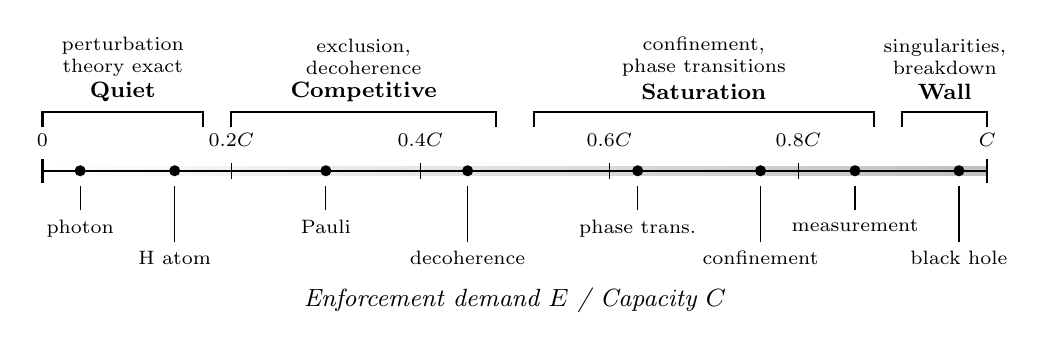
\begin{tikzpicture}[x=12cm, y=1cm]

% --- Gradient shading (behind everything) ---
\shade[left color=white, right color=black!25] (0,-0.06) rectangle (1,0.06);

% --- Main axis ---
\draw[thick] (0,0) -- (1,0);
\draw[thick] (0,-0.15) -- (0,0.15);
\draw[thick] (1,-0.15) -- (1,0.15);

% Tick marks + labels ABOVE axis
\foreach \x/\lab in {0/{0}, 0.2/{0.2$C$}, 0.4/{0.4$C$}, 0.6/{0.6$C$}, 0.8/{0.8$C$}, 1.0/{$C$}} {
  \draw (\x,-0.1) -- (\x,0.1);
  \node[above, font=\scriptsize] at (\x,0.18) {\lab};
}

% --- Regime brackets ---
\draw[thick] (0,0.55) -- (0,0.75) -- (0.17,0.75) -- (0.17,0.55);
\node[font=\footnotesize\bfseries] at (0.085,1.0) {Quiet};
\node[font=\scriptsize, text width=2cm, align=center] at (0.085,1.45) {perturbation\\theory exact};

\draw[thick] (0.20,0.55) -- (0.20,0.75) -- (0.48,0.75) -- (0.48,0.55);
\node[font=\footnotesize\bfseries] at (0.34,1.0) {Competitive};
\node[font=\scriptsize, text width=2.6cm, align=center] at (0.34,1.45) {exclusion,\\decoherence};

\draw[thick] (0.52,0.55) -- (0.52,0.75) -- (0.88,0.75) -- (0.88,0.55);
\node[font=\footnotesize\bfseries] at (0.70,1.0) {Saturation};
\node[font=\scriptsize, text width=2.6cm, align=center] at (0.70,1.45) {confinement,\\phase transitions};

\draw[thick] (0.91,0.55) -- (0.91,0.75) -- (1.0,0.75) -- (1.0,0.55);
\node[font=\footnotesize\bfseries] at (0.955,1.0) {Wall};
\node[font=\scriptsize, text width=1.6cm, align=center] at (0.955,1.45) {singularities,\\breakdown};

% --- System markers: staggered rows ---
\fill (0.04,0) circle (2pt);
\draw (0.04,-0.2) -- (0.04,-0.5);
\node[below, font=\scriptsize, anchor=north] at (0.04,-0.5) {photon};

\fill (0.30,0) circle (2pt);
\draw (0.30,-0.2) -- (0.30,-0.5);
\node[below, font=\scriptsize, anchor=north] at (0.30,-0.5) {Pauli};

\fill (0.63,0) circle (2pt);
\draw (0.63,-0.2) -- (0.63,-0.5);
\node[below, font=\scriptsize, anchor=north] at (0.63,-0.5) {phase trans.};

\fill (0.86,0) circle (2pt);
\draw (0.86,-0.2) -- (0.86,-0.5);
\node[below, font=\scriptsize, anchor=north] at (0.86,-0.5) {measurement};

\fill (0.14,0) circle (2pt);
\draw (0.14,-0.2) -- (0.14,-0.9);
\node[below, font=\scriptsize, anchor=north] at (0.14,-0.9) {H atom};

\fill (0.45,0) circle (2pt);
\draw (0.45,-0.2) -- (0.45,-0.9);
\node[below, font=\scriptsize, anchor=north] at (0.45,-0.9) {decoherence};

\fill (0.76,0) circle (2pt);
\draw (0.76,-0.2) -- (0.76,-0.9);
\node[below, font=\scriptsize, anchor=north] at (0.76,-0.9) {confinement};

\fill (0.97,0) circle (2pt);
\draw (0.97,-0.2) -- (0.97,-0.9);
\node[below, font=\scriptsize, anchor=north] at (0.97,-0.9) {black hole};

% Axis label
\node[font=\small\itshape] at (0.5,-1.65) {Enforcement demand $E$ / Capacity $C$};

% Redraw axis endpoints
\draw[thick] (0,-0.15) -- (0,0.15);
\draw[thick] (1,-0.15) -- (1,0.15);

\end{tikzpicture}

\medskip
\caption{The enforcement spectrum.  Physical systems arranged by the ratio of enforcement demand to capacity ($E/C$).  Standard physics works exactly in the quiet regime ($E/C \ll 1$), requires approximations in the competitive regime ($E/C$ of order unity), and breaks down---singularities, the measurement problem, the information paradox---at the capacity wall ($E/C \to 1$).  The hard problems of physics cluster where $E/C \to 1$.  Regime boundaries are schematic.}
\label{fig:spectrum}
\end{figure}

\medskip\noindent\textbf{The quiet regime ($E/C \ll 1$).}
A single photon maintains two polarization states; a hydrogen atom holds a handful of quantum numbers with well-separated energy levels.  Nothing competes for resources.  Perturbation theory converges, exact solutions exist, and QED predicts the electron's anomalous magnetic moment to 12 decimal places~\cite{Aoyama2020}.  The physics is simple because the budget is barely taxed.

\medskip\noindent\textbf{The competitive regime ($E/C$ of order unity, below saturation).}
The budget begins to bind.  Two electrons cannot maintain identical quantum numbers because the joint enforcement cost overflows the local budget---the Pauli exclusion principle \emph{is} non-closure.  Decoherence appears because system--environment correlations commit capacity at both interfaces, and the committed capacity is locally unrecoverable~\cite{Zurek2003}.  Perturbation theory still works but requires increasingly sophisticated approximations: the system is managing genuine competition for finite resources.

\medskip\noindent\textbf{The saturation regime ($E/C$ approaching unity).}
The budget is nearly exhausted and the physics becomes dramatic.  In QCD, a free quark's unscreened color charge costs more to enforce the further it separates; when the cost exceeds interface capacity, the string snaps and produces color-singlet hadrons---fewer distinctions, lower demand~\cite{Wilson1974}.  At a phase transition, thermal perturbation costs consume the enforcement budget for the ordered state until the system can no longer afford it and transitions to disorder~\cite{Wilson1983}.  In measurement, cross-system correlations multiply as apparatus and environment entangle, saturating the budget until only one branch survives~\cite{Zurek1981}.

\medskip\noindent\textbf{The capacity wall ($E/C \to 1$).}
The Bekenstein--Hawking bound $S = A/4\ell_P^2$~\cite{Bekenstein1981} and the APF's $n_{\max} = \lfloor C/\varepsilon^* \rfloor$ are both finite-capacity bounds on the number of independent physical facts a region can support.  The structural parallel is suggestive, but the quantitative mapping ($\varepsilon^* = \alpha\ell_P^2$, gravitational scaling from enforcement capacity) is the subject of Papers~5--6, not this paper.

\medskip\noindent\textbf{The pattern.}  The standard formalism works beautifully in the quiet regime, requires approximations in the competitive regime, and breaks down---singularities, the measurement problem, the information paradox---at the capacity wall.  The APF's interpretive proposal is that these are not separate problems but manifestations of a single structural feature: the formalism has no finite enforcement budget and cannot describe what happens when the budget runs out.  A1 supplies that concept.  Whether this interpretive proposal can be made quantitative --- reproducing known scalings in controlled settings --- is the subject of Papers~5--6, not this paper.


\subsection{Context: reconstruction and finite-information programs}
\label{sec:context}

The APF enters a well-established tradition.  Since Hardy's reconstruction of quantum theory from five operational axioms~\cite{Hardy2001}, a sustained program --- Chiribella, D'Ariano, and Perinotti~\cite{CDP2011}; Masanes and M\"uller~\cite{MM2011}; Dakic and Brukner~\cite{DakicBrukner2009} --- has sought to derive the Hilbert-space formalism from physically motivated principles rather than assume it.  These programs start from a specified mathematical setting (generalized probabilistic theories) and impose operational axioms until quantum theory is the unique solution.  The APF answers a prior question: \emph{why should physics be a GPT at all?}  A1 derives the convex-probabilistic structure that GPTs assume, and A1 + MD derive the mathematical setting itself (convexity, linearity, finite dimensionality, noncommutativity).

The following table gives a systematic cross-reference.  Standard GPT/reconstruction axioms are listed in the left column; the right column gives their APF status --- derived, not needed, or replaced by a different mechanism.  No GPT axiom is assumed by the APF; those that appear in peer programs are either proved as theorems or replaced by enforcement-specific results.

\smallskip
\begin{center}
\captionof{table}{GPT reconstruction axioms and their APF status.}
\smallskip
\footnotesize
\begin{tabular}{@{}p{4.0cm}p{1.4cm}p{7.2cm}@{}}
\textbf{GPT / reconstruction axiom} & \textbf{Status} & \textbf{APF source} \\[2pt]
\hline\noalign{\smallskip}
Convex state space & Derived & OR1 (Prop.~OR1): A1's real-valued budget $\Rightarrow$ convex mixing of strategies \\[3pt]
Finite dimensionality & Derived & OR3 ($T_{\mathrm{form}}$): A1 + MD + SC $\Rightarrow$ $\dim S_\Gamma < \infty$ \\[3pt]
Local tomographic closure & Derived & $P_{\mathrm{tom}}$ (Section~\ref{sec:skeleton}): $L_{\mathrm{loc}}$ + $\mathcal{D}$-quotient \\[3pt]
Compositional closure / purification & Derived & $P_{\mathrm{cls}}$ (Section~\ref{sec:skeleton}): $L_{\mathrm{loc}}$ + A1 \\[3pt]
Continuous reversibility (Hardy) & Not needed & Replaced by $T_{\mathrm{adj}}$: self-adjointness from cost symmetry; no Lie-group axiom \\[3pt]
Purification (CDP) & Not needed & Follows from T2 + $T_{\mathrm{tensor}}$ once Hilbert space is derived \\[3pt]
Self-adjoint observables (OR2) & Derived & $T_{\mathrm{adj}}$: idempotency + $T_{\mathrm{sep}}$ + cost additivity $\Rightarrow$ $E_d = E_d^\dagger$ \\[3pt]
No-signaling & Derived & $T_{\mathrm{NS}}$: corollary of $L_{\mathrm{loc}}$ (budget independence) \\[3pt]
No-broadcasting & Derived & $T_{\mathrm{NB}}$: from $T_{\mathrm{alg}}$ (noncommutativity) + $T_M$ (monogamy) \\[3pt]
Born rule / frame functions & Derived & $T_{\mathrm{Born}}$: Gleason/Busch applied to the derived algebra; hypotheses (NC, OA, affineness) all verified from $T_{\mathrm{sep}}$, $L_{\mathrm{cost}}$, and GNS \\
\end{tabular}
\label{tab:gpt_crossref}
\end{center}

\smallskip\noindent The Born rule deserves specific comment.  Peer programs derive it either from the GPT framework's built-in state-effect pairing (which assumes convexity, finite-dimensionality, and tomographic completeness) or from Gleason's theorem applied to a pre-existing Hilbert space.  The APF uses neither route in its assumed form: it derives the algebra (T2a), derives the Hilbert space (T2b), derives the positive faithful state $\omega$ (O4, from enforcement costs), verifies Busch's four hypotheses (non-contextuality from $T_{\mathrm{sep}}$; ortho-additivity from $L_{\mathrm{cost}}$; normalization from budget accounting; affineness from GNS linearity), and then invokes Busch's theorem --- which applies in all dimensions $\ge 1$, avoiding Gleason's $\dim \ge 3$ restriction.  The GPT structures that other programs need as starting axioms for the Born rule (convexity, tomographic closure, frame-function existence) are all available as derived results when $T_{\mathrm{Born}}$ is invoked; they enter as proved theorems, not as assumptions.

A1 is closest in spirit to the finite-information tradition in quantum gravity: Bekenstein's entropy bound~\cite{Bekenstein1981}, the holographic principle ('t~Hooft~\cite{tHooft1993}, Susskind~\cite{Susskind1995}), and Jacobson's thermodynamic derivation of Einstein's equations~\cite{Jacobson1995}.  A1 can be read as the common ancestor: a primitive statement that enforcement resources are finite, from which both the quantum formalism and (in the companion papers) the gravitational structure follow as consequences.

What is new is the novel chain $L_\Delta \to L_{\mathrm{blk}} \to T_{\mathrm{alg}}$ (with geometric strengthening $L_\Pi$), which has no counterpart in peer programs: it derives noncommutativity from enforcement costs without assuming any algebraic structure.  Every piece of linear geometry used in the bridge --- the inner product, orthogonal projections, Grassmannian compactness --- is constructed from the cost functional before it is used, not smuggled in from a pre-existing Hilbert space; the derivation order and non-circularity are traced in the Linear Structure Provenance table (Box~\ref{box:provenance}) and independently verified via sequential effect algebras in Appendix~\ref{app:sea}.  The three standard steps that complete the derivation ($T_{\mathrm{embed}}$, $T_{\mathrm{GNS}}$, T2c) are presented with full proofs (Section~\ref{sec:precise_scope}).  Two conditions that reconstruction programs take as axioms --- local tomographic closure ($P_{\mathrm{tom}}$) and compositional closure ($P_{\mathrm{cls}}$) --- are here proved as theorems.  The CBH constraints (no-signaling, no-broadcasting) emerge as corollaries.  Detailed comparisons with individual programs (CBH, Spekkens, Connes NCG, Barnum--Wilce, CQM, resource theories, LOCC frameworks, and generalized noncontextuality) are given in Appendix~I.

\subsection{The APF engine: code as specification}

Every theorem in this paper series is implemented as an executable check function in the APF codebase---a modular Python package organized by derivation layer (\texttt{core}, \texttt{gauge}, \texttt{generations}, \texttt{spacetime}, \texttt{gravity}, \texttt{cosmology}).  Each check function encodes the theorem's statement, verifies its numerical content against exact arithmetic (using Python's \texttt{Fraction} type), records its dependencies, and returns a structured result.  A separate validation module compares derived predictions to experimental benchmarks (Planck 2018~\cite{Planck2018}, PDG 2024~\cite{PDG2024}, NuFit 6.0~\cite{NuFit2024}) behind a firewall that isolates empirical data from the derivation chain.  Code references of the form \texttt{(check\_X, module.py)} appear throughout Papers 1--7.  The codebase is publicly available at \url{https://github.com/Ethan-Brooke}.


\subsection{Road map: from axiom to physics}

\noindent\textit{A self-contained narrative walkthrough of the complete argument---readable in 15 minutes, with enough mathematical content to assess each step---is given in Section~\ref{sec:argument}.  The tables below serve as quick reference for locating specific results by name.}

\medskip
This paper establishes the axiom and derives five structural lemmas ($L_{\varepsilon^*}$, $L_{\mathrm{loc}}$, $L_{\mathrm{nc}}$, $L_\Delta$, $L_{\mathrm{irr}}$) from A1, the structural assumption MD (Enforcement Isotropy), the definitions of Section~\ref{sec:defs}, and stated richness premises.  The derivation order is strict and acyclic:

\begin{center}
\captionof{table}{Derivation order of the structural lemmas and bridge theorems.  Rows 7--11 constitute the bridge; the chain's multi-step structure answers the classical-countermodel objection.}
\smallskip
\footnotesize
\setlength{\tabcolsep}{3pt}
\begin{tabular}{@{}cp{2.6cm}p{1.2cm}p{4.0cm}p{3.0cm}@{}}
\toprule
\textbf{\#} & \textbf{Result} & \textbf{Type} & \textbf{Dependencies} & \textbf{Used by} \\
\midrule
1 & $L_{\mathrm{NZ}}$ (No Zeno) & Lemma & A1 (Aspect~3) & motivation \\
2 & $L_{\varepsilon^*}$ (Min.\ Cost) & Lemma & MD & all below \\
3 & $L_{\mathrm{loc}}$ (Locality) & Lemma & A1, $L_{\varepsilon^*}$, M, $R_{\mathrm{loc}}$ & $L_{\mathrm{irr}}$, Papers 2--7 \\
4 & $L_{\mathrm{nc}}$ (Non-Closure) & Lemma & A1, $L_{\varepsilon^*}$, M & $L_{\mathrm{irr}}$, T1 \\
5 & $L_{\Delta}$ (Competition) & Lemma & A1, SC, CL1--CL3, $T_{\mathrm{sep}}$ & T1, $L_{\mathrm{irr}}$ \\
6 & $L_{\mathrm{irr}}$ (Irreversibility) & Lemma & $L_{\mathrm{nc}}$, $L_\Delta$, $L_{\mathrm{loc}}$ & Papers 3--5 \\
\midrule
\multicolumn{5}{l}{\textit{Bridge: from order-dependence to noncommutative $C^*$-algebra}} \\
\midrule
7 & T1 (Order-Dep.) & Thm & $L_\Delta$, NT, BW & O2 \\
8 & $T_{\mathrm{adj}}$ / OR2 & Thm & $T_{\mathrm{sep}}$, cost additivity & $L_{\mathrm{blk}}$, $L_\Pi$, $T_{\mathrm{alg}}$ \\
8b & $L_{\mathrm{blk}}$ (Direct-Sum Realiz.) & Thm & $T_{\mathrm{sep}}$, SC, A1, $L_\Delta$ & $T_{\mathrm{alg}}$ (critical path) \\
9 & $L_\Pi$ (Codespace Rot.) & Lemma & $L_\Delta$, OR3, $T_{\mathrm{adj}}$ & FD6 (geometric strengthening) \\
10 & $T_{\mathrm{alg}}$ (Noncomm.) & Thm & $L_{\mathrm{blk}}$, OR2 & T2a \\
11 & $T_{\mathrm{GNS}}$ & Thm & T2a (O3, O4) & T2b, T2c \\
\bottomrule
\end{tabular}
\label{tab:deriv_order}
\end{center}

These feed into the quantum skeleton: T2a (real $*$-algebra) $\to$ T2b (complexification + Wedderburn--Artin) $\to$ T2c (field selection $\mathbb{C}$).  The bridge rows 7--11 are the multi-step argument that crosses the boundary from operational order-dependence (satisfiable by classical models) to algebraic noncommutativity (not satisfiable by any commutative $*$-algebra).  The classical-countermodel objection is addressed at row~8: $T_{\mathrm{adj}}$ places the enforcement operators \emph{inside} $\mathcal{A}$ as self-adjoint elements; classical models keep their update maps external to the observable algebra, so no self-adjoint enforcement-internal update operator exists (Proposition~CME, Section~\ref{sec:operator_bridge}).


\smallskip\noindent The full assumption inventory (one axiom (A1), one structural assumption (MD), one richness premise (BW), and constitutive/derived definitions) is tabulated in Section~\ref{sec:assumption_inventory}.

\subsubsection*{Derivation order}

The derivation has two independent branches that converge at T2.

\medskip
\noindent\textbf{Branch 1: quantum structure.}\enspace{}
A1 forces $L_{\mathrm{nc}}$ (state space is not closed) and $L_\Delta$ (co-location costs are strictly superadditive).  Superadditivity forces order-dependence in enforcement (T1).

\textbf{T1 alone does not force noncommutativity}: classical Bayesian conditioning also exhibits order-dependent updates (explicit countermodel in the T1 box, Section~\ref{sec:L_Delta}).  The passage from T1 to a noncommutative $C^*$-algebra requires three further steps, each proved in Section~\ref{sec:operator_bridge}:
\begin{enumerate}[nosep,leftmargin=2em,itemsep=4pt]
\item \textit{Self-adjointness.}\enspace{} $T_{\mathrm{adj}}$ derives the $*$-involution ($E_d = E_d^\dagger$) from cost symmetry.  Classical models have a $*$-operation on $\ell^\infty(X)$ (complex conjugation), but their update maps (Bayesian conditioning) are \emph{not elements of} $\ell^\infty(X)$ --- they are stochastic matrices in $\mathrm{End}(\Delta(X))$.  The APF places enforcement operators inside $\mathcal{A}$; in any commutative algebra, internal self-adjoint elements commute, contradicting T1 (Prop.~CME).
\item \textit{Direct-sum realizability.}\enspace{} $L_{\mathrm{blk}}$ proves the biconditional: $\Delta > 0$ iff every admissible joint defender requires nontrivial $\Pi$-support (failure of direct-sum realizability).  The corollary gives an explicit commutator witness.  (The geometric strengthening $L_\Pi$ shows this $\Pi$-support arises from codespace rotation.)
\item \textit{Noncommutativity.}\enspace{} $T_{\mathrm{alg}}$ proves $[E_{d_1}, F_\Pi] \ne 0$ and shows no faithful commutative $*$-representation exists.
\end{enumerate}
The GNS construction ($T_{\mathrm{GNS}}$, exhibited step-by-step for the general case) then delivers the Hilbert-space representation~(T2).

\medskip
\noindent\textbf{Branch 2: locality and gauge.}\enspace{}
A1 forces $L_{\mathrm{loc}}$ (independent interfaces have independent budgets).  Independent-budget interfaces, once T2 identifies the algebra as a sum of matrix algebras over $\mathbb{C}$, have automorphism groups classified by Skolem--Noether as inner automorphisms --- i.e., conjugation by unitary elements.  This is the structural origin of gauge symmetry: the automorphism type (unitary group) is determined by T2 + Skolem--Noether within this paper; the specific gauge group ($SU(3) \times SU(2) \times U(1)$) is determined by the budget deployment across the 61 capacity channels (Paper~2).

\medskip
\noindent\textbf{Independence.}\enspace{}
The two branches do not depend on each other: $L_{\mathrm{loc}}$ does not require $L_\Delta$, and $L_\Delta$ does not require $L_{\mathrm{loc}}$.  The critical path to Hilbert space runs through $L_\Delta$, not $L_{\mathrm{loc}}$.  The complete dependency structure is shown in Figure~\ref{fig:dag}.


\label{sec:axiom}
% ======================================================================

\subsubsection*{The three inputs}

The entire framework rests on three stated inputs.  All subsequent structure --- definitions, lemmas, theorems --- is derived from these three and nothing else.  The complete dependency graph is shown in Figure~\ref{fig:dag}; the detailed physical grounding of each input appears in Section~\ref{sec:defs}.

\medskip
\noindent\textbf{Axiom A1} (Finite Enforcement Capacity) is the sole physical axiom.

\smallskip\noindent\textit{Every physical fact costs something to maintain, and the total is bounded.}

\smallskip\noindent A1's structural content is scarcity.  A finite budget means distinctions compete for resources.  Without a bound, any collection of distinctions could coexist without mutual interference --- no exclusion, no superadditivity, no order-dependence, no noncommutativity.  The budget is what makes maintaining one distinction affect the affordability of maintaining another.  That mutual interference is the structural origin of everything downstream: $L_\Delta$ (superadditivity) exists because two distinctions sharing a finite substrate must defend against joint perturbations that cost more than the sum of their individual defenses.  T1 (order-dependence) exists because enforcing $d_1$ before $d_2$ leaves a different residual budget than the reverse.  The Heisenberg uncertainty relation, at the end of the chain, is a consequence of residual budgets: conjugate distinctions cannot be simultaneously maintained because their joint enforcement cost overflows the interface capacity.  A1 does not specify what the structure looks like; it imposes the scarcity that forces structure to emerge.

\begin{tcolorbox}[apfbox, title={Axiom A1 (Finite Enforcement Capacity)}]
\textbf{Physicality criterion.}
Within this framework, a distinction is physically real iff maintaining it requires strictly positive enforcement cost.  For a state $\sigma$ on a causally connected region $R$, the raw domain of physically real distinctions is
\[
\mathcal{D}(\sigma,R)
\;:=\;
\{\, d \;:\; d \text{ is maintained in } (\sigma,R)\ \text{and}\ \varepsilon(d)>0 \,\}.
\]

\textbf{Budget bound.}
For any admissible state $\sigma$ on a causally connected region $R$, at least two physically real distinctions are simultaneously maintainable, and their total enforcement cost is finite:
\[
|\mathcal{D}(\sigma,R)| \ge 2,
\qquad
\sum_{d \in \mathcal{D}(\sigma,R)} \varepsilon(d)
\;\le\;
C(R)
\;<\;
\infty.
\]

\smallskip\noindent\textbf{\textit{Variables:}}
\begin{varlist}
\item $\Omega$ --- the abstract state set: the collection of all possible configurations of enforced distinctions.  No algebraic or topological structure is assumed on $\Omega$ at this stage.
\item $\sigma \in \Omega$ --- a state (a particular configuration of enforced distinctions on region $R$).
\item $R$ --- a causally connected region of the universe.
\item $\mathcal{D}(\sigma,R)$ --- the raw domain of physically real distinctions maintained in state $\sigma$ on region $R$: all maintained distinctions $d$ with $\varepsilon(d)>0$.  Later results may impose additional structural conditions on subfamilies of $\mathcal{D}(\sigma,R)$ when exact capacity accounting is required.
\item $\varepsilon(d)$ --- the enforcement cost of distinction $d$: the minimum capacity required to maintain $d$ against admissible perturbation.  Positivity, $\varepsilon(d)>0$, is the membership condition for $\mathcal{D}(\sigma,R)$.  No global lower bound is asserted here; that is the content of $L_{\varepsilon^*}$.
\item $C(R)$ --- the total enforcement capacity of region $R$: the finite upper bound on how much enforcement can be simultaneously committed within $R$.
\end{varlist}

\smallskip\noindent\textbf{Note on $|\mathcal{D}| \ge 2$.}
The condition $|\mathcal{D}(\sigma,R)| \ge 2$ is the minimal non-vacuity requirement for a theory of maintained distinctions: with fewer than two, no distinction structure exists for the budget bound to govern.  Paper~2 confirms that this presupposition is satisfied by the framework's own field content.

\smallskip\noindent\textbf{Status.}  \textbf{[Axiom]} --- the single physical postulate of the framework.  All other results are derived from A1 plus the structural assumption MD and constitutive definitions FD1--FD6.

\coderef{check\_A1}{paper1.py}
\end{tcolorbox}

\medskip
\noindent\textbf{Assumption MD} (Enforcement Isotropy) is the single structural assumption beyond A1.

\smallskip\noindent\textit{The enforcer has no built-in preferred directions --- every irreducible distinction costs at least $\mu^* > 0$.}

\smallskip\noindent MD is often written as $\varepsilon(d) \ge \mu^* \cdot n(d)$, which looks like it assumes linear scaling with the number of binary tests.  It does not.  The linear appearance is a compact repackaging of two logically independent facts:

\smallskip\noindent\textbf{MD's actual content (the assumption):} Every irreducible distinction --- one requiring a single binary test --- costs at least $\mu^* > 0$ to maintain, uniformly: no test is cheaper than any other.  This is isotropy: the enforcer has no preferred directions.

\smallskip\noindent\textbf{Why the linear bound follows (not assumed):}  A distinction with enforcement complexity $n(d)$ decomposes into $n(d)$ irreducible sub-tests with disjoint anchor sets.  Disjoint anchor sets have additive costs ($T_{\mathrm{sep}}$, proved from A1 alone).  Each sub-test costs $\ge \mu^*$ (MD).  Therefore $\varepsilon(d) \ge n(d) \cdot \mu^*$.  The ``linear scaling'' is not a structural commitment to linearity --- it is independence (from A1) plus a per-test floor (the real content of MD).

\smallskip\noindent Without MD, you could have an enforcer that cheaply maintains $\hat{z}$-spin and expensively maintains $\hat{x}$-spin; that would hard-code a preferred axis into the foundations, which is exactly what the framework derives (via $L_{\mathrm{blk}}$, $L_\Pi$, and T2) rather than assumes.  MD is the condition that keeps the enforcer structureless so that the physics it enforces can acquire structure honestly.

\begin{tcolorbox}[defbox, title={Assumption MD (Enforcement Isotropy)}]
\label{box:MD_formal}

\textbf{Statement.}
There exists $\mu^* > 0$ such that every irreducible distinction (enforcement complexity $n(d) = 1$) satisfies
\[
\varepsilon(d) \;\ge\; \mu^*.
\]
That is: the per-test enforcement cost has a positive floor, uniform across all distinctions and all degrees of freedom.

\medskip\noindent\textbf{Derived consequence (linear bound).}
For any distinction $d$ with enforcement complexity $n(d) \ge 1$:
\[
\varepsilon(d) \;\ge\; \mu^* \cdot n(d).
\]

\smallskip\noindent\textit{Derivation.}  The $n(d)$ sub-tests of $d$ are independently enforceable by construction ($n(d)$ is the \emph{minimum} count; redundant tests would reduce it).  Independent distinctions have disjoint anchor sets, so $T_{\mathrm{sep}}$ (from A1) gives cost additivity: $\varepsilon(d) \ge \sum_{i=1}^{n(d)} \varepsilon(t_i)$.  MD gives $\varepsilon(t_i) \ge \mu^*$ for each sub-test $t_i$.  Therefore $\varepsilon(d) \ge n(d) \cdot \mu^*$.  The linear scaling is a theorem of A1 + MD, not an additional assumption.

\medskip\noindent\textbf{Immediate consequence.}
Since $n(d) \ge 1$ for every non-trivial distinction, MD gives a uniform floor: $\varepsilon^* := \inf_d \varepsilon(d) \ge \mu^* > 0$.  This is $L_{\varepsilon^*}$ (Section~\ref{sec:logical_status_eps_star}).

\smallskip\noindent\textbf{\textit{Variables:}}
\begin{varlist}
\item $n(d)$ --- the \emph{enforcement complexity} of distinction $d$: the minimum number of independent binary tests required to specify $d$'s enforcement status.  Before the vector-space structure is established, $n(d)$ is a combinatorial quantity (binary-test count on $\Omega$); after FD1b, $n(d) = \dim(M_d)$.
\item $\mu^*$ --- the \emph{per-test cost floor}: the minimum enforcement cost per binary test, uniform across all distinctions.  $\mu^* > 0$ is the single free constant in MD; its value is never needed (only its positivity matters).
\item $\varepsilon^*$ --- the \emph{minimum enforcement cost}: $\varepsilon^* := \inf_{d \in \mathcal{D}} \varepsilon(d) \ge \mu^* > 0$.  Derived from MD, not assumed independently.
\end{varlist}

\smallskip\noindent\textbf{What MD does not assume.}
MD does not assert linear cost structure, convexity, or any geometric property.  It asserts a single scalar inequality: every irreducible test costs at least $\mu^*$.  The linear bound $\varepsilon(d) \ge n(d) \cdot \mu^*$ is a \emph{consequence} of this floor combined with cost additivity ($T_{\mathrm{sep}}$, from A1).  Costs above the floor can be arbitrarily context-dependent: a qubit in a 10T field costs more than one in a 1T field; both cost $\ge \mu^*$.  Non-additive costs arise for co-located distinctions competing for shared resources ($L_\Delta$, $\Delta > 0$) --- this is where the framework's quantum content lives, and MD does not suppress it.

\smallskip\noindent\textbf{Note on physical corroboration.}
The isotropy pattern --- same cost per binary test regardless of which test --- appears across disparate physical domains: the qubit energy gap $g\mu_B B$ (independent of spin axis); stabilizer-code syndrome overhead (independent of which generator); the Bekenstein--Hawking bound ($\ell_P^2$ per distinction, independent of physical nature); Landauer's principle ($k_BT\ln 2$ per bit, independent of which bit).  The alternative --- an enforcer whose cost varies arbitrarily across DOFs --- requires preferred internal structure that A1's pre-geometric state space $\Omega$ does not possess.  Full discussion, countermodel, and comparison with reconstruction-program assumptions: Section~\ref{assumption:MD}.

\coderef{check\_MD}{paper1.py}
\end{tcolorbox}

\medskip
\noindent\textbf{Richness Premise BW} (Budget Window) is the sole richness condition.

\smallskip\noindent\textit{The cost spectrum is rich enough that different enforcement orderings produce distinguishable outcomes.}

\smallskip\noindent BW's structural content is spectral richness.  A1 and MD together give a finite budget with a uniform cost floor, but that alone permits trivially symmetric worlds: two distinctions of equal cost on a single interface satisfy A1 and MD while remaining perfectly commutative --- no ordering asymmetry, no budget-window witness, no detectable noncommutativity.  BW prevents this degenerate case.  It requires the cost spectrum to contain at least one triple $(d_1, d_2, d_3)$ where $d_3$ fits alongside the cheaper $d_1$ but overflows alongside the more expensive $d_2$.  This is what makes $L_\Delta$'s superadditive surplus operationally visible: enforce $d_1$ first, then $d_3$ succeeds; enforce $d_2$ first, then $d_3$ fails.  The residual budgets differ, and a physical experiment can tell which ordering occurred.  BW is the minimum spectral complexity that converts the algebraic noncommutativity forced by A1 into a physically observable phenomenon.

\begin{tcolorbox}[defbox, title={Richness Premise BW (Budget Window)}]
\label{box:BW_formal}

\textbf{Spectral richness condition.}
The cost spectrum $\{\varepsilon(d) : d \in \mathcal{D}\}$ contains at least one witnessing triple: there exist $d_1, d_2, d_3 \in \mathcal{D}$ with $\varepsilon(d_1) < \varepsilon(d_2)$ such that $d_3$ is jointly admissible with $d_1$ but not with $d_2$:
\[
\varepsilon(\{d_1, d_3\}) \;\le\; C \quad\text{and}\quad \varepsilon(\{d_2, d_3\}) \;>\; C.
\]

\textbf{Where BW enters.}
BW is used exactly once: in the proof of T1 (order-dependence, Section~\ref{sec:L_Delta}).  It provides the third distinction $d_3$ that witnesses the residual-budget asymmetry created by $L_\Delta$'s superadditive surplus.  No other theorem in this paper requires BW.

\smallskip\noindent\textbf{\textit{Variables:}}
\begin{varlist}
\item $(d_1, d_2, d_3)$ --- the \emph{BW triple}: three distinctions in $\mathcal{D}$ with $\varepsilon(d_1) < \varepsilon(d_2)$ and $d_3$ in the budget window between the two co-located pairs $\{d_1, d_3\}$ and $\{d_2, d_3\}$.
\item $\varepsilon(\{d_i, d_j\})$ --- the \emph{joint enforcement cost} of maintaining $d_i$ and $d_j$ simultaneously, including any superadditive surplus $\Delta(d_i, d_j)$ from $L_\Delta$.
\item $(C - \varepsilon(d_2),\; C - \varepsilon(d_1)]$ --- the \emph{budget window}: the interval in which $\varepsilon(d_3)$ must fall for the triple to witness order-dependence.
\end{varlist}

\smallskip\noindent\textbf{Note on confirmation.}
BW is the only premise not derived from A1 within this paper.  It is confirmed by Paper~2's derivation of 61 independent capacity types, which provides far more witnessing triples than needed.  Within Paper~1, the worked example (Section~\ref{sec:worked_example}) exhibits a concrete satisfying instance with $C = 5$, $\varepsilon(d_1) = 1$, $\varepsilon(d_2) = 2$, $\varepsilon(d_3) = 3.5$.

\coderef{check\_BW}{paper1.py}
\end{tcolorbox}

\smallskip\noindent\textbf{On the ``single-axiom'' framing and the acronym proliferation.}
A reader encountering the derivation chain will meet numerous labelled items --- SC, CL1--CL3, $T_{\mathrm{sep}}$, NT, OR0--OR3, FD1--FD6, K1--K4, P1--P4 --- and may reasonably ask whether these are covert additional axioms.  They are not, but the concern deserves a direct answer.  The items fall into exactly three categories, none of which is an independent physical postulate:

\emph{(i) Constitutive definitions} (FD1--FD6, K1--K4, OR0).  These define the vocabulary: what a distinction is (FD1--FD2), what an anchor set is (FD3), what a perturbation costs (FD4, K1--K4), what an enforcement operation does (FD5--FD6), and what ``state'' means (OR0).  They are the formal spelling-out of A1's English sentence ``the cost of maintaining distinctions is bounded.''  Every reconstruction program has an analogous definitional layer (Hardy's ``states, effects, transformations''; CDP's ``systems, tests, channels''); the APF's is longer because it operates pre-geometrically.

\emph{(ii) Derived conditions} (OR1--OR3, SC, $T_{\mathrm{sep}}$, NT, CL1--CL3, P1--P4).  Each is proved as a theorem from A1 + MD + the definitions.  OR1 (convex mixing) is derived from A1's real-valued budget.  OR2 (self-adjointness) is Theorem $T_{\mathrm{adj}}$.  OR3 (finite dimensionality) is Theorem $T_{\mathrm{form}}$.  SC (Substrate Completeness) is derived from MD + $\mathcal{D}$-quotient.  $T_{\mathrm{sep}}$ (disjoint anchors $\Leftrightarrow$ additive costs) is proved from FD3 + A1.  NT (non-degeneracy) is a corollary of $L_{\mathrm{cost}}$.  CL1--CL3 (co-location conditions for $L_\Delta$) are geometric properties derived from $n_{\max} \ge 3$ (which follows from OR3).  P1--P4 (perturbation lemmas) are proved from A1 + $T_{\mathrm{sep}}$ + OR3.  The complete derivation status of each item is tabulated in Section~\ref{sec:assumption_inventory} (Tables~\ref{tab:critical_path}--\ref{tab:derived_items}).

\emph{(iii) The three genuine inputs} (A1, MD, BW).  These are stated above: one axiom, one structural assumption, one richness premise.  Everything else in the paper traces back to them through a proved chain.

The ``single-axiom'' claim is therefore precise: A1 is the sole physical axiom.  MD is a structural assumption (analogous to Hardy's continuous reversibility or CDP's purification --- not a physical law but a regularity condition excluding pathological countermodels).  BW is a richness premise (analogous to Hardy's simplicity or CDP's tomographic completeness --- confirming the cost spectrum is non-degenerate).  The definitional layer is long because the paper defines its primitives from scratch rather than importing the GPT framework; the derived-condition layer is long because the paper proves as theorems what peer programs assume as axioms.  Neither layer adds physical content beyond A1 + MD + BW.


\subsection*{Reader's guide}


The Formal Specifications in Section~\ref{sec:defs} are reference cards; the proofs are distributed across the paper in dependency order.  This guide maps every key claim to its proof, explains the paper's two-branch structure, and indicates which sections can be skipped on a first reading.

\medskip\noindent\textbf{Where to find each proof.}  For a reviewer checking a specific claim:

\smallskip
\renewcommand{\arraystretch}{1.25}
\begin{tabular}{@{}p{3.5cm}p{2.6cm}p{6.3cm}@{}}
\textbf{Claim} & \textbf{Location} & \textbf{What to look for} \\[2pt]
\hline\noalign{\smallskip}
$\varepsilon^* > 0$ ($L_{\varepsilon^*}$) & Sec.~\ref{sec:logical_status_eps_star} & Two-step proof from MD; no physics \\[2pt]
Disjoint $\Leftrightarrow$ separated ($T_{\mathrm{sep}}$) & Sec.~\ref{sec:defs} & Biconditional; both directions proved \\[2pt]
Self-adjointness ($T_{\mathrm{adj}}$, OR2) & Sec.~\ref{sec:operator_bridge} & Five-step proof; Step~3 (sector-orthogonal bilinear form) = $L_\omega$ in Formal Supplement \\[2pt]
Superadditivity ($L_\Delta$) & Sec.~\ref{sec:L_Delta} & Substrate-integrity argument (4 steps) + LP verification + toy model \\[2pt]
Order-dependence (T1) & Sec.~\ref{sec:L_Delta} & Three-operation witness (3 steps) + Bayesian countermodel \\[2pt]
Bridge to noncommutativity & Sec.~\ref{sec:operator_bridge} & $L_{\mathrm{blk}}$: biconditional (excess cost $\Leftrightarrow$ failure of direct-sum realizability); $L_\Pi$: geometric strengthening with explicit witness; $T_{\mathrm{alg}}$: $[E_{d_1}, F_\Pi] \ne 0$, no commutative $*$-rep \\[2pt]
GNS construction ($T_{\mathrm{GNS}}$) & Sec.~\ref{sec:T2} & Six-step general case (G1--G6) + hypothesis verification table \\[2pt]
Field selection $\mathbb{C}$ (T2c) & Sec.~\ref{sec:T2c} & $K = N^2$ count; $\mathbb{R}$-exclusion via $P_{\mathrm{tom}}$; $\mathbb{H}$-exclusion via Brauer group \\[2pt]
Born rule ($T_{\mathrm{Born}}$) & Sec.~\ref{sec:T2} & Gleason/Busch applied to derived algebra; hypotheses verified \\[2pt]
Tsirelson bound & Sec.~\ref{sec:T_Tsirelson} & Cirel'son operator identity in the derived Hilbert space \\[2pt]
Cost uniqueness ($L_{\mathrm{cost}}$) & Sec.~\ref{sec:L_cost} & Cauchy equation on $\mathbb{N}$; induction; Boltzmann analogy \\[2pt]
Novel predictions & Sec.~\ref{box:empirical_content} & Three categories; crossover formula Eq.~\eqref{eq:crossover} \\[2pt]
Full pipeline (A1 $\to$ Born) & Sec.~\ref{sec:T2} & End-to-end worked trace \\[2pt]
Scope and status of each result & Sec.~\ref{sec:precise_scope} & Table~\ref{tab:scope}: proved / conditional / deferred \\[2pt]
Complete assumption inventory & Sec.~\ref{sec:assumption_inventory} & Three inputs (A1, MD, BW); everything else derived \\
\end{tabular}

\medskip\noindent\textbf{Paper structure: two branches converging at T2.}

\smallskip\noindent\textit{Branch 1 (quantum structure, critical path):} A1 $\to$ $L_{\varepsilon^*}$ $\to$ $L_\Delta$ $\to$ T1 $\to$ $T_{\mathrm{adj}}$ $\to$ $L_{\mathrm{blk}}$ $\to$ $T_{\mathrm{alg}}$ $\to$ $T_{\mathrm{GNS}}$ $\to$ T2.  This is the enforcement-to-Hilbert-space chain.  The novel content ($L_\Delta \to L_{\mathrm{blk}} \to T_{\mathrm{alg}}$) has no counterpart in peer reconstruction programs; $L_\Pi$ provides geometric strengthening but is not on the critical path.

\smallskip\noindent\textit{Branch 2 (locality and gauge):} A1 $\to$ $L_{\mathrm{loc}}$ $\to$ Skolem--Noether (after T2).  This branch produces gauge symmetry.  It does not depend on Branch~1 until T2 is available.

\smallskip\noindent The two branches share no intermediate results: $L_{\mathrm{loc}}$ does not require $L_\Delta$, and $L_\Delta$ does not require $L_{\mathrm{loc}}$.

\medskip\noindent\textbf{Suggested reading orders.}

\smallskip\noindent\textit{For the conceptual argument (15 min):} Section~1 (motivation) $\to$ Section~\ref{sec:walkthrough} (accessible walkthrough of the bridge) $\to$ Section~\ref{sec:scope} (scope).

\smallskip\noindent\textit{For mathematical verification:} Section~\ref{sec:defs} (definitions, structural lemmas) $\to$ Section~\ref{sec:formal_bridge} (the formal bridge: $L_\Delta$, T1, $T_{\mathrm{adj}}$, $L_{\mathrm{blk}}$, $T_{\mathrm{alg}}$, GNS, T2a--T2c, Born rule, Tsirelson bound --- all proofs self-contained).

\smallskip\noindent\textit{Sections safe to skip on first reading:} \S1.2 (enforcement spectrum), \S1.4 beyond the first three paragraphs (detailed literature comparisons), Section~\ref{sec:consequences} (consequences and applications), Appendices A--H.

\medskip\noindent\textbf{Seven worked examples} provide pencil-and-paper checkpoints: the finite worked example (\S\ref{sec:worked_example}, $C=5$, three distinctions), the overlapping-mechanisms counterexample (\S\ref{sec:defs}), the LP verification of $L_\Delta$ (\S\ref{sec:L_Delta}), the $M_2(\mathbb{C})$ witness (Corollary to $T_{\mathrm{alg}}$), the GNS construction for the enforcement algebra (\S\ref{sec:T2}), the stabilizer-code mapping (\S\ref{sec:L_cost}), and the transmon protocol (\S\ref{box:empirical_content}).

\smallskip
\begin{center}
\captionof{table}{Worked examples and toy models: pencil-and-paper checkpoints.}
\smallskip
\renewcommand{\arraystretch}{1.25}
\begin{tabular}{@{}p{3.8cm}p{2.5cm}p{6.1cm}@{}}
\textbf{Example} & \textbf{Location} & \textbf{What it demonstrates} \\[2pt]
\hline\noalign{\smallskip}
Two competing distinctions ($C = 5$, three distinctions) & Sec.~\ref{sec:worked_example} & Explicit $L_\Delta$ verification ($\Delta = 4$); BW satisfied; P1--P4 checked numerically; order-dependent residuals exhibited \\[3pt]
Overlapping mechanisms ($S_\Gamma = \mathbb{R}^2$, $M_{d_2} \subset M_{d_1}$) & Sec.~\ref{sec:defs} & $T_{\mathrm{sep}}$ fails; $\Delta = -\varepsilon^* < 0$; every bridge link breaks; algebra is $\mathbb{R}^2$ (commutative). Concrete counterexample to ``order effects $\Rightarrow$ noncommutativity'' \\[3pt]
Full pipeline witness ($d_1 = \sigma_z$, $d_2 = \sigma_x$) & Sec.~\ref{sec:T2} & A1 $\to$ $L_\Delta$ $\to$ T1 $\to$ T2 $\to$ GNS $\to$ Born rule in explicit matrices; $[A,B] = -2i\sigma_y$; Gram eigenvalues; Gleason applied \\[3pt]
Enforcement cone ($M_2(\mathbb{C})$) & Sec.~\ref{sec:T2} & PSD cone constructed; self-duality proved ($K = K^*$); homogeneity via $g = B^{1/2}A^{-1/2}$; SDR verified \\[3pt]
$\mathbb{R}$-exclusion ($N{=}M{=}2$) & Sec.~\ref{sec:T2c} & Joint params $= 9$, local $= 8$; antisymmetric correlator identified; $P_{\mathrm{tom}}$ violated \\[3pt]
$\mathbb{H}$-exclusion (Brauer) & Sec.~\ref{sec:T2c} & $\mathbb{H} \otimes_\mathbb{R} \mathbb{H} \cong M_4(\mathbb{R})$; center argument; composite exits quaternionic class \\[3pt]
$C^*$-axiom verification table & Sec.~\ref{sec:operator_bridge} & Each $C^*$-axiom (norm, involution, $C^*$-identity, completeness) listed with its source; GNS prerequisites (four items) verified explicitly \\[3pt]
Decoherence protocols (transmon + trapped ion) & Sec.~\ref{box:experimental_protocol} & Crossover formula Eq.~\eqref{eq:crossover}; fit functions; null vs.\ APF discriminator; $N_E$-scaling \\
\end{tabular}
\label{tab:worked_examples}
\end{center}




\clearpage
\begin{figure}[p]
\centering
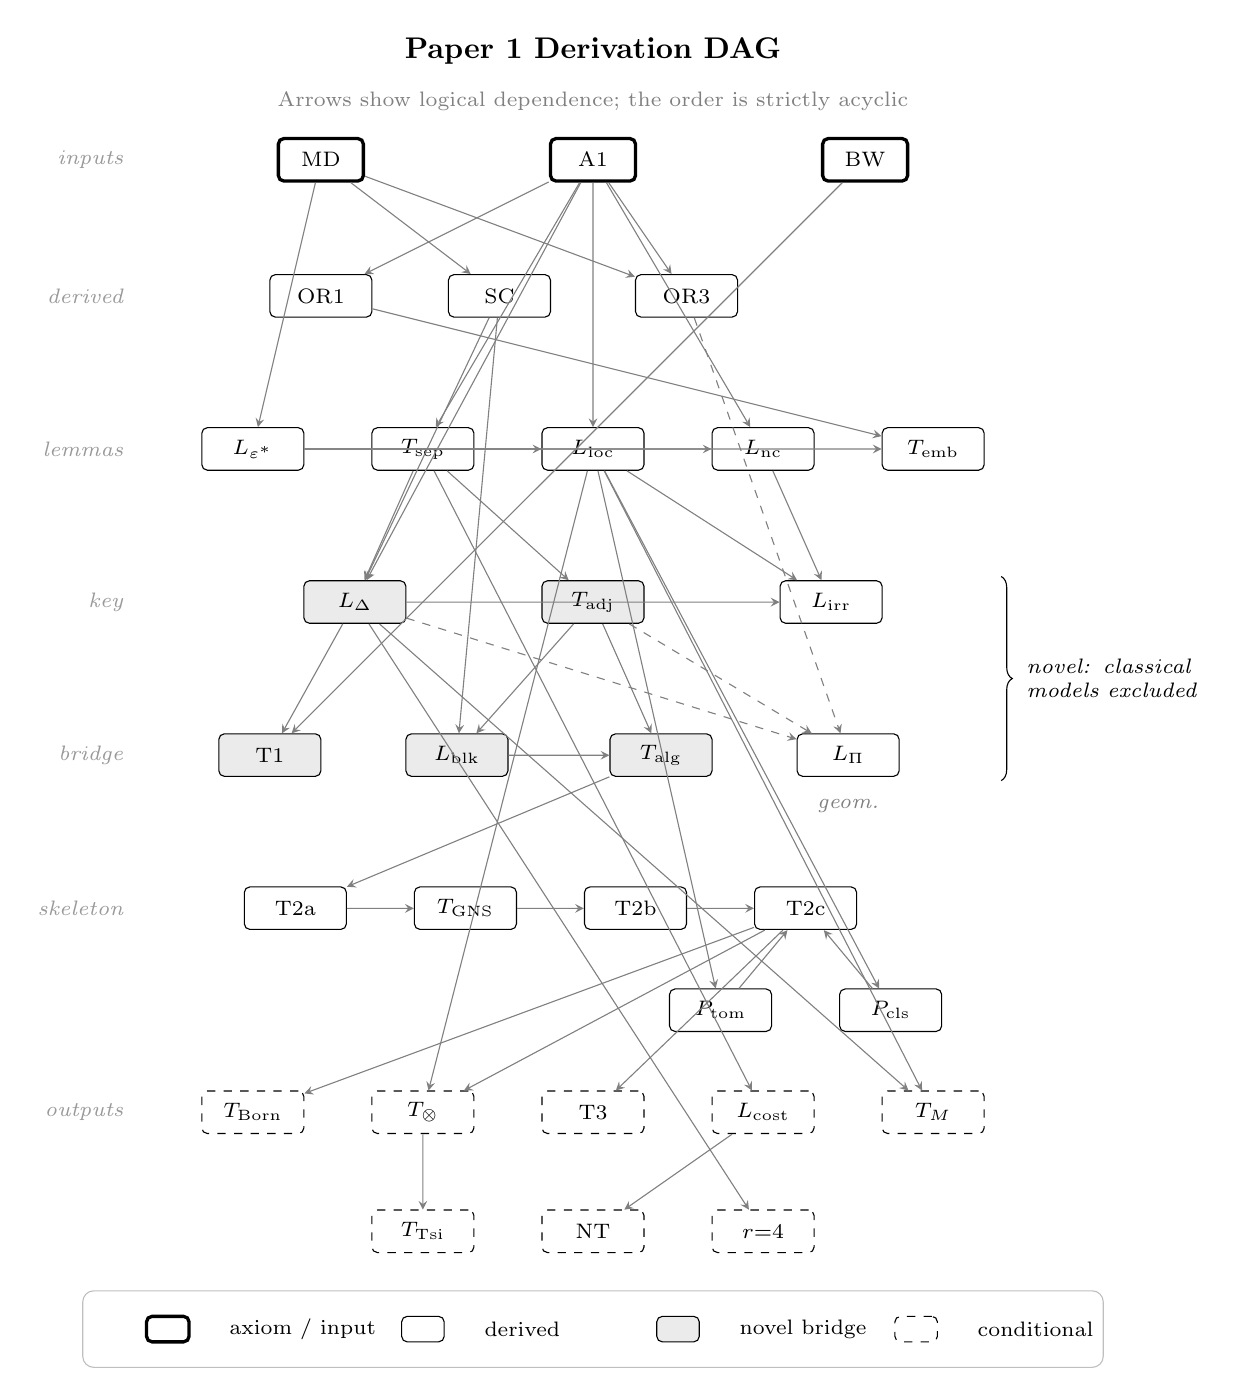
\begin{tikzpicture}[
    scale=1.08, every node/.style={transform shape},
    nd/.style={draw, rounded corners=2pt, minimum height=0.5cm, minimum width=1.2cm, inner sep=2pt, font=\scriptsize},
    input/.style={nd, very thick, minimum width=1.0cm},
    lemma/.style={nd},
    bridge/.style={nd, fill=black!8},
    skel/.style={nd},
    outnode/.style={nd, dashed},
    arr/.style={->, >=stealth, thin, black!50},
    tier/.style={font=\tiny\itshape, anchor=east, text=black!40},
]

% Title
\node[font=\normalsize\bfseries, anchor=south] at (0, 1.0) {Paper 1 Derivation DAG};
\node[font=\scriptsize, anchor=south, text=black!50] at (0, 0.45) {Arrows show logical dependence; the order is strictly acyclic};

% Tier 0: Inputs
\node[tier] at (-5.4, 0) {\scriptsize inputs};
\node[input] (A1) at (0, 0) {A1};
\node[input] (MD) at (-3.2, 0) {MD};
\node[input] (BW) at (3.2, 0) {BW};

% Tier 1: Derived conditions
\node[tier] at (-5.4, -1.6) {\scriptsize derived};
\node[lemma] (OR1) at (-3.2, -1.6) {OR1};
\node[lemma] (SC) at (-1.1, -1.6) {SC};
\node[lemma] (OR3) at (1.1, -1.6) {OR3};

% Tier 2: Structural lemmas
\node[tier] at (-5.4, -3.4) {\scriptsize lemmas};
\node[lemma] (Leps) at (-4.0, -3.4) {$L_{\varepsilon^*}$};
\node[lemma] (Tsep) at (-2.0, -3.4) {$T_{\mathrm{sep}}$};
\node[lemma] (Lloc) at (0.0, -3.4) {$L_{\mathrm{loc}}$};
\node[lemma] (Lnc) at (2.0, -3.4) {$L_{\mathrm{nc}}$};
\node[lemma] (Temb) at (4.0, -3.4) {$T_{\mathrm{emb}}$};

% Tier 2.5: Key lemmas
\node[tier] at (-5.4, -5.2) {\scriptsize key};
\node[bridge] (LDelta) at (-2.8, -5.2) {$L_\Delta$};
\node[bridge] (Tadj) at (0.0, -5.2) {$T_{\mathrm{adj}}$};
\node[lemma] (Lirr) at (2.8, -5.2) {$L_{\mathrm{irr}}$};

% Tier 3: Bridge
\node[tier] at (-5.4, -7.0) {\scriptsize bridge};
\node[bridge] (T1) at (-3.8, -7.0) {T1};
\node[bridge] (Lblk) at (-1.6, -7.0) {$L_{\mathrm{blk}}$};
\node[bridge] (Talg) at (0.8, -7.0) {$T_{\mathrm{alg}}$};
\node[lemma] (LPi) at (3.0, -7.0) {$L_\Pi$};
\node[font=\scriptsize\itshape, gray, anchor=north] at (3.0, -7.4) {geom.};

% Annotation: novel bridge (right side)
\draw[decorate, decoration={brace, amplitude=4pt}]
    (4.8, -4.9) -- (4.8, -7.3)
    node[midway, right=5pt, font=\scriptsize\itshape, text width=2.2cm, align=left] {novel: classical\\models excluded};

% Tier 4: Skeleton
\node[tier] at (-5.4, -8.8) {\scriptsize skeleton};
\node[skel] (T2a) at (-3.5, -8.8) {T2a};
\node[skel] (TGNS) at (-1.5, -8.8) {$T_{\mathrm{GNS}}$};
\node[skel] (T2b) at (0.5, -8.8) {T2b};
\node[skel] (T2c) at (2.5, -8.8) {T2c};

% Derived for T2c
\node[lemma] (Ptom) at (1.5, -10.0) {$P_{\mathrm{tom}}$};
\node[lemma] (Pcls) at (3.5, -10.0) {$P_{\mathrm{cls}}$};

% Tier 5: Consequences
\node[tier] at (-5.4, -11.2) {\scriptsize outputs};
\node[outnode] (TBorn) at (-4.0, -11.2) {$T_{\mathrm{Born}}$};
\node[outnode] (Ttens) at (-2.0, -11.2) {$T_{\otimes}$};
\node[outnode] (T3) at (0.0, -11.2) {T3};
\node[outnode] (Lcost) at (2.0, -11.2) {$L_{\mathrm{cost}}$};
\node[outnode] (TM) at (4.0, -11.2) {$T_M$};

% Terminal
\node[outnode] (Ttsi) at (-2.0, -12.6) {$T_{\mathrm{Tsi}}$};
\node[outnode] (NT) at (0.0, -12.6) {NT};
\node[outnode] (r4) at (2.0, -12.6) {$r{=}4$};

% === ARROWS ===
% Tier 0 → 1
\draw[arr] (A1) -- (OR1);
\draw[arr] (MD) -- (SC);
\draw[arr] (MD) -- (OR3);
\draw[arr] (A1) -- (OR3);

% Tier 0/1 → 2
\draw[arr] (MD) -- (Leps);
\draw[arr] (A1) -- (Tsep);
\draw[arr] (A1) -- (Lloc);
\draw[arr] (Leps) -- (Lloc);
\draw[arr] (A1) -- (Lnc);
\draw[arr] (Leps) -- (Lnc);
\draw[arr] (OR1) -- (Temb);
\draw[arr] (Leps) -- (Temb);

% → key lemmas
\draw[arr] (SC) -- (LDelta);
\draw[arr] (Tsep) -- (LDelta);
\draw[arr] (A1) -- (LDelta);
\draw[arr] (Tsep) -- (Tadj);
\draw[arr] (LDelta) -- (Lirr);
\draw[arr] (Lnc) -- (Lirr);
\draw[arr] (Lloc) -- (Lirr);

% → bridge
\draw[arr] (LDelta) -- (T1);
\draw[arr] (BW) -- (T1);
\draw[arr] (Tadj) -- (Lblk);
\draw[arr] (SC) -- (Lblk);
\draw[arr] (Lblk) -- (Talg);
\draw[arr] (Tadj) -- (Talg);
\draw[arr, gray, dashed] (LDelta) -- (LPi);
\draw[arr, gray, dashed] (Tadj) -- (LPi);
\draw[arr, gray, dashed] (OR3) -- (LPi);

% bridge → skeleton
\draw[arr] (Talg) -- (T2a);
\draw[arr] (T2a) -- (TGNS);
\draw[arr] (TGNS) -- (T2b);
\draw[arr] (T2b) -- (T2c);
\draw[arr] (Ptom) -- (T2c);
\draw[arr] (Pcls) -- (T2c);
\draw[arr] (Lloc) -- (Ptom);
\draw[arr] (Lloc) -- (Pcls);

% skeleton → outputs
\draw[arr] (T2c) -- (TBorn);
\draw[arr] (T2c) -- (Ttens);
\draw[arr] (Lloc) -- (Ttens);
\draw[arr] (T2c) -- (T3);
\draw[arr] (Tsep) -- (Lcost);
\draw[arr] (Lloc) -- (TM);
\draw[arr] (LDelta) -- (TM);

% → terminal
\draw[arr] (Ttens) -- (Ttsi);
\draw[arr] (Lcost) -- (NT);
\draw[arr] (LDelta) -- (r4);

% === LEGEND ===
\draw[black!25, rounded corners=4pt] (-6.0, -14.2) rectangle (6.0, -13.3);
\node[input, minimum width=0.5cm, minimum height=0.3cm] at (-5.0, -13.75) {};
\node[font=\scriptsize, anchor=west] at (-4.4, -13.75) {axiom / input};
\node[lemma, minimum width=0.5cm, minimum height=0.3cm] at (-2.0, -13.75) {};
\node[font=\scriptsize, anchor=west] at (-1.4, -13.75) {derived};
\node[bridge, minimum width=0.5cm, minimum height=0.3cm] at (1.0, -13.75) {};
\node[font=\scriptsize, anchor=west] at (1.6, -13.75) {novel bridge};
\node[outnode, minimum width=0.5cm, minimum height=0.3cm] at (3.8, -13.75) {};
\node[font=\scriptsize, anchor=west] at (4.4, -13.75) {conditional};

\end{tikzpicture}
\caption[Paper~1 Derivation DAG]{%
\textbf{Paper~1 Derivation DAG.}
Every arrow is a logical dependency; the graph is strictly acyclic.
The three inputs (thick border) are
\textbf{A1}~(Finite Enforcement Capacity),
\textbf{MD}~(Enforcement Isotropy),
and \textbf{BW}~(Budget Window); all other nodes are derived.
The shaded bridge chain ($L_\Delta \to T_{\mathrm{adj}} \to L_{\mathrm{blk}} \to T_{\mathrm{alg}}$) is the novel core of the paper: this is where all classical models are excluded.  ($L_\Pi$ provides geometric strengthening but is not on the critical path.)
Two independent branches --- quantum structure (left, via~$L_\Delta$) and locality/gauge (right, via~$L_{\mathrm{loc}}$) --- converge at T2c.
Dashed nodes are conditional on the identifications of \S\ref{sec:identifications}.
}
\label{fig:dag}
\end{figure}
\clearpage

% ======================================================================

% ======================================================================
\section{Definitions and structural lemmas}
\label{sec:defs}
% ======================================================================

\subsection{Physical grounding of the three inputs}
\label{sec:input_grounding}

The three inputs (A1, MD, BW) are stated formally in Section~\ref{sec:axiom}.  This subsection provides their detailed physical interpretation, the relationship between A1's two internal regimes, and the argument for positivity at zero temperature.  All material here is interpretive --- no theorem depends on it --- but it grounds the formal machinery in physical intuition.


\medskip\noindent\textit{A1's Two Internal Regimes.}
\label{cor:disjoint_mech}
A1 governs the raw domain $\mathcal{D}(\sigma,R)$ of all maintained distinctions with positive enforcement cost.  The budget bound $\sum_{d} \varepsilon(d) \le C(R)$ holds over any finite subfamily, but its meaning depends on the geometric relationship between enforcement mechanisms:

\textbf{When mechanisms overlap} ($M_{d_1} \cap M_{d_2} \ne \{0\}$ for some pair): the budget sum \emph{overcounts} shared substrate.  The actual capacity consumed by the pair is less than $\varepsilon(d_1) + \varepsilon(d_2)$; the inequality is a loose upper bound, not an exact accounting.  Superadditivity ($L_\Delta$, $\Delta > 0$) does not hold.  The enforcement structure is additive or sub-additive --- the classical knapsack model, where adding more distinctions is always affordable as long as individual costs fit.

\textbf{When mechanisms are disjoint} ($M_{d_1} \cap M_{d_2} = \{0\}$ for all pairs, i.e., the subfamily is in $\mathcal{D}_{\mathrm{ind}}$): the budget sum is an \emph{exact} accounting --- it equals the capacity actually consumed.  Each distinction draws on an independent substrate segment.  In this regime: superadditivity holds ($\Delta > 0$, from the substrate-integrity argument, Section~\ref{sec:L_Delta}); the enforcement algebra is noncommutative (T1); and the full quantum structure follows (T2).

Both regimes are genuine physical regimes within A1's scope, not an inside/outside split.  $T_{\mathrm{sep}}$ is the structural theorem that characterizes when a maintained family lies in the exact-accounting regime.  It does not add physics to A1; it identifies the geometric condition under which A1's budget bound sharpens from an inequality to an equality, and in doing so unlocks the derivation chain from finite capacity to quantum mechanics.


This is a constraint on what nature can do, not on what we can observe.  The specific value of $C$ is never required; only finiteness and positivity matter.

\smallskip\noindent\textbf{Physical interpretation of A1.}
The inequality $\sum \varepsilon(d) \le C < \infty$ has three aspects whose physical content is worth separating.

\textit{Aspect 1 (Total budget is finite).}  This is the literal content of A1.  It is the only formal constraint.

\textit{Aspect 2 (Each maintained distinction is realized by a finite act with positive cost).}  This is the content of $\varepsilon(d) > 0$ for each $d \in \mathcal{D}$.  A distinction that costs nothing to maintain is not being enforced in any physical sense; under A1, enforcement capacity is consumed by maintenance, so zero-cost distinctions lie outside the framework's scope.  This aspect has physical corroboration in Landauer's principle~\cite{Landauer1961}: erasing (or maintaining against erasure) one bit of information dissipates at least $k_B T \ln 2$ of energy.  Enforcement is not thermodynamically free.  Note that Landauer's bound is temperature-dependent and goes to zero as $T \to 0$; it therefore corroborates per-distinction positivity at $T > 0$ but does not supply a universal, temperature-independent floor.

\smallskip\noindent\textit{Why $\varepsilon(d) > 0$ at $T = 0$.}  Enforcement cost is not Landauer's thermodynamic erasure cost.  Landauer's bound $k_B T \ln 2$ quantifies the minimum \emph{thermal} dissipation for erasure against a heat bath at temperature $T$; it vanishes at $T = 0$ because there is no thermal noise to overcome.  Enforcement cost $\varepsilon(d)$ quantifies the minimum capacity required to maintain $d$ against \emph{all admissible perturbations} $\mathcal{P}(d)$, not just thermal ones.  At $T = 0$, the relevant perturbations are quantum vacuum fluctuations (zero-point energy $\tfrac{1}{2}\hbar\omega > 0$), which are strictly positive and temperature-independent.  A distinction maintained against vacuum fluctuations costs positive capacity even at absolute zero.

Three concrete examples confirm this.  (i)~A qubit in a magnetic field at $T = 0$: the energy gap $g\mu_B B > 0$ is the enforcement cost, set by the field magnitude, not the temperature.  Vacuum fluctuations can induce transitions across this gap; maintaining the spin state requires the gap to be present.  (ii)~A superconducting transmon at $T \to 0$: the Josephson energy $E_J > 0$ and the charging energy $E_C > 0$ together set the qubit frequency $\omega_{01} = \sqrt{8E_J E_C} - E_C > 0$.  The qubit is operational precisely because this gap is nonzero at $T = 0$; the gap \emph{is} the enforcement cost.  (iii)~The Bekenstein--Hawking bound $S = A/4\ell_P^2$: the maximum number of independently enforceable distinctions for area $A$ is temperature-independent; each costs $\varepsilon^* = C/N = 4\ell_P^2 C/A > 0$ regardless of the black hole's Hawking temperature.

The reconciliation is therefore: Landauer's principle addresses the \emph{thermal component} of enforcement cost, which vanishes at $T = 0$.  The APF's $\varepsilon(d) > 0$ addresses the \emph{total} enforcement cost, which includes a temperature-independent quantum component (zero-point energy, vacuum fluctuations, geometric bounds) that remains strictly positive at all temperatures.  MD's floor $\mu^* > 0$ is the formal expression of this: the per-complexity enforcement cost is bounded below by a constant that does not depend on temperature.

\textit{Aspect 3 (Enforcement histories are Zeno-free).}  Finite total capacity does not by itself prevent a convergent series of ever-smaller enforcement acts: $\sum_{n=1}^\infty 2^{-n} = 1$ shows that infinitely many distinctions with costs $1/2, 1/4, 1/8, \ldots$ fit within a budget of 1.  What physically prevents this is that enforcement is a \emph{realizable commitment process}, not merely a numerical budget.  A physical act of enforcement cannot be infinitely subdivided; there is a smallest scale at which enforcement can occur.  This is the operational content of Aspect~3, and it is the physically motivated ground for the no-Zeno lemma ($L_{\mathrm{NZ}}$) below.  $L_{\mathrm{NZ}}$ establishes that no admissible enforcement \emph{history} contains a Zeno sequence; the uniform positive floor $\varepsilon^* > 0$ on the set $\mathcal{D}$ itself is proved as a theorem in Section~\ref{sec:logical_status_eps_star} via MD (Enforcement Isotropy): $\varepsilon(d) \ge \mu^* \cdot n(d) \ge \mu^*$ for every $d \in \mathcal{D}$, where $n(d) \ge 1$ is the enforcement complexity (minimum binary tests to specify $d$'s status; see Section~\ref{assumption:MD}).  Paper~6 additionally derives the dimensional value $\varepsilon^* = \alpha\ell_p^2$ from the Bekenstein--Hawking entropy bound~\cite{Bekenstein1981}, providing a physical scale; that identification is not needed for any result in this paper.

\smallskip\noindent\textbf{What A1 is not.}
A1 does not say how large $C$ is.  It does not say what the distinctions are made of.  It does not say whether the universe is classical or quantum, continuous or discrete, four-dimensional or otherwise.  All of those properties are derived in Sections~\ref{sec:defs}--\ref{sec:skeleton} as consequences of the axiom, not written into it.

The axiom is not a simplifying assumption.  If enforcement resources are unlimited, there is no cap on how many distinctions can be maintained.  If there is no cap, then every conceivable pattern can persist---nothing is forced to give way.  If nothing is forced, there are no constraints.  And if there are no constraints, there is no physics: no selection, no structure, no law.  Finite enforceability is the minimum condition for physical law to exist.


\smallskip\noindent\textbf{Assumption MD (Enforcement Isotropy).}
\label{assumption:MD}

\textit{Pre-geometric formulation (used in the derivation).}  For each distinction $d \in \mathcal{D}$, define its \emph{enforcement complexity} $n(d)$ as the minimum number of independent binary tests required to fully determine the enforcement status of $d$ (whether $d$ is active, what budget it consumes, what residual it leaves).  MD asserts:
\[
\boxed{\text{There exists } \mu^* > 0 \text{ such that } \varepsilon(d) \;\geq\; \mu^* \cdot n(d) \quad \text{for every } d \in \mathcal{D}.}
\]
The enforcement complexity $n(d)$ is defined on the abstract state space $\Omega$ (FD0) and does not reference any vector space, inner product, or linear structure.  It is a purely operational quantity: the minimum number of yes/no questions needed to specify $d$'s enforcement status.  For every $d \in \mathcal{D}$, $n(d) \ge 1$ (a non-trivial binary predicate requires at least one test).  Therefore MD gives $\varepsilon(d) \ge \mu^* \cdot 1 = \mu^* > 0$ uniformly.

\textit{Post-geometric equivalence (confirmed after $T_{\mathrm{form}}$).}  Once OR3 establishes $\dim S_\Gamma < \infty$ and the canonical embedding identifies $\Omega$ with a convex subset of $V = \mathbb{R}^{N+1}$, the enforcement complexity $n(d)$ coincides with the linear-algebraic dimension $\dim(M_d)$ of the anchor subspace $M_d \subseteq S_\Gamma$.  The identification is: each independent binary test corresponds to a linearly independent direction in $M_d$; the minimum number of such tests is the dimension.  In this setting, MD reads $\varepsilon(d) \ge \mu^* \cdot \dim(M_d)$, which is the form used in all downstream results.  The coincidence is \emph{confirmed} by the vector-space construction, not presupposed by it.

\smallskip\noindent\textit{Dependency order and non-circularity of MD.}
\begin{enumerate}[nosep,leftmargin=2em,itemsep=2pt]
\item A1 defines $\Omega$ (abstract state set) with enforcement operations $\mathfrak{e}_d$.
\item MD is stated using $n(d)$ (enforcement complexity, defined on $\Omega$, no vector space required).
\item MD $\Rightarrow$ $L_{\varepsilon^*}$: $\varepsilon^* := \inf_d \varepsilon(d) \ge \mu^* > 0$ (uniform floor from $n(d) \ge 1$).
\item OR1 (from real-valued $C$) $+$ $L_{\varepsilon^*}$ $\Rightarrow$ canonical embedding $\varphi: \Omega \hookrightarrow \mathbb{R}^{N+1}$ with $N \le \lfloor C/\varepsilon^* \rfloor < \infty$ (Proposition~\ref{prop:FD1_derived}).
\item OR3 ($T_{\mathrm{form}}$, from MD + SC + A1): $\dim S_\Gamma \le C/\mu^* < \infty$.
\item \textbf{After} Step~5: the vector-space structure is in place, and $n(d) = \dim(M_d)$ is confirmed.
\end{enumerate}
\noindent MD enters at Step~2 using only the operational quantity $n(d)$; $\dim(M_d)$ first appears at Step~6.  No circularity.

MD is the single structural assumption beyond A1 in this paper.  Its precise content is worth isolating.

\smallskip\noindent\textit{What MD says.}  Every unit of enforcement complexity costs at least $\mu^*$ to maintain, \emph{uniformly across all distinctions}.  The per-test enforcement cost is distinction-independent: a distinction requiring one binary test incurs cost $\ge \mu^*$, regardless of which test it is.  After the vector space is constructed, this reads: the per-dimension enforcement cost is direction-independent.

\smallskip\noindent\textit{What MD rules out (explicit countermodel).}  Consider an interface $\Gamma$ with infinitely many irreducible distinctions $d_n$ (each requiring one binary test, so $n(d_n) = 1$) with costs $\varepsilon(d_n) = 1/2^n$.  Every individual cost is strictly positive, costs are additive on independent distinctions, and the total budget $C = \sum_{n=1}^\infty 1/2^n = 1 < \infty$ (A1 holds).  But $\varepsilon^* = \inf_n 1/2^n = 0$: there is no uniform positive floor, and the interface supports infinitely many independent distinctions.  In this countermodel, some distinctions are exponentially cheaper to maintain than others despite having the same enforcement complexity $n(d_n) = 1$.  MD excludes this by requiring a complexity-independent cost floor.


\smallskip\noindent\textit{MD's logical status --- a sharper characterization.}
The companion paper \emph{Markov Breakdown and the Hard Problems} (MB) supplies a
stronger characterization of MD's place in the assumption inventory.  Three routes
to deriving MD from A1 were assessed and all three fail.  (i)~Budget-exhaustion
via QEC protection: if $\varepsilon^* = 0$, QEC (forced by FD6) must protect
against arbitrarily cheap erasures; but protection costs are sequential, not
additive, and do not contradict $C < \infty$.  (ii)~$L_{\mathrm{NZ}}$: the
no-Zeno lemma governs enforcement histories, not static budget allocations; the
countermodel $\varepsilon(d_n) = 1/2^n$ involves simultaneous maintenance costs,
not a temporal sequence.  (iii)~QEC code dimensionality via FD6: FD6 is proved
after OR3 which requires MD; using FD6 to derive MD is circular.  The countermodel
stands.

What MB establishes instead is an equivalence that reframes MD's physical content
without changing its logical status.  Under A1 and $L_{\mathrm{loc}}$:
\[
  \text{MD}
  \;\Longleftrightarrow\;
  \exists\,\sigma \text{ on } ABC :
  \Delta_{\mathrm{SSA}}(\sigma) = 0,
\]
where $\Delta_{\mathrm{SSA}} = \varepsilon_{AC} + \varepsilon_{ABC}$ is the
enforcement Markov gap and $\Delta_{\mathrm{SSA}} = 0$ is the enforcement Markov
condition (interface $B$ screens $A$ from $C$ with zero cross-gap budget).  Without
MD ($\varepsilon^* = 0$), every state has $\Delta_{\mathrm{SSA}} > 0$: cross-gap
enforcement at zero marginal cost appears in every configuration, the Markov
condition never holds, and physics has no quiet regime.  The contrapositive is
sharp: \emph{a universe in which MD fails is a universe without simple cases} ---
perturbation theory never converges, and the Standard Model approximation is never
valid.

The equivalence gives MD a second physical reading alongside the substrate
formulation above.  Substrate formulation: ``each unit of enforcement complexity
costs at least $\mu^* > 0$, uniformly.''  Structural formulation: ``there exist
physical states in which the Markov condition holds exactly.''  Both are equivalent
under A1 $+$ $L_{\mathrm{loc}}$; the structural formulation is the one the Markov
theory makes natural.  Full derivation in MB, Section~4 ($T_{\mathrm{QEC\text{-}Markov}}$) and Section~3 ($L_{\mathrm{SSA}}$).

\smallskip\noindent\textit{What MD does not say.}  MD does not assert that all distinctions with the same complexity have exactly the same cost; it asserts a \emph{lower bound} per unit of complexity.  The exact cost $\varepsilon(d) = n(d) \cdot \varepsilon^*$ (equality rather than inequality) is the stronger conclusion of $L_{\mathrm{cost}}$ (the Cauchy uniqueness theorem), which uses $T_{\mathrm{sep}}$'s additive independence.  MD provides only the floor; $L_{\mathrm{cost}}$ sharpens it to equality.

\smallskip\noindent\textit{Detailed discussion of MD} (countermodels, non-circularity under coarse-graining and composition, comparison with peer-program assumptions, the factored-route alternative) \textit{is in Section~\ref{sec:MD_detail}.  No bridge proof depends on that discussion.}

\smallskip\noindent\textbf{Richness Premise BW (Budget Window).}

\textit{Physical grounding.}  A1 and MD together provide a finite budget with a uniform cost floor.  But that alone permits trivially symmetric configurations: two distinctions of equal cost satisfy A1 and MD while remaining perfectly commutative --- no ordering asymmetry, no observable noncommutativity.  BW is the minimum condition that prevents this degeneracy.

\smallskip\noindent\textit{What BW says.}  The cost spectrum $\{\varepsilon(d) : d \in \mathcal{D}\}$ contains at least one witnessing triple $(d_1, d_2, d_3)$ with $\varepsilon(d_1) < \varepsilon(d_2)$ such that $d_3$ is jointly admissible with the cheaper $d_1$ but not with the more expensive $d_2$: $\varepsilon(\{d_1,d_3\}) \le C$ and $\varepsilon(\{d_2,d_3\}) > C$.  The distinction $d_3$ lives in the \emph{budget window} --- the interval of costs that fit alongside one enforcement commitment but overflow alongside another.  When such a triple exists, the residual budget after enforcing $d_1$ is detectably different from the residual after enforcing $d_2$: enforce $d_1$ first, then $d_3$ succeeds; enforce $d_2$ first, then $d_3$ fails.  A physical experiment can tell which ordering occurred.

\smallskip\noindent\textit{What BW rules out.}  Without BW, all distinctions could have the same cost $\varepsilon(d) = \varepsilon^*$, and every enforcement ordering would leave the same residual budget.  The algebraic noncommutativity forced by $L_\Delta$ would be present in the abstract algebra but invisible to any physical measurement: no probe distinction could witness the ordering asymmetry.  BW converts abstract algebraic noncommutativity into physically observable order-dependence.

\smallskip\noindent\textit{Where BW enters.}  BW is used exactly once: in the proof of T1 (order-dependence, Section~\ref{sec:L_Delta}).  It provides the third distinction $d_3$ that witnesses the residual-budget asymmetry created by $L_\Delta$'s superadditive surplus.  No other theorem in this paper requires BW.

\smallskip\noindent\textit{Confirmation.}  BW is the only premise not derived from A1 within this paper.  It is confirmed by Paper~2's derivation of 61 independent capacity types, which provides far more witnessing triples than needed.  The worked example (Section~\ref{sec:worked_example}) exhibits a concrete satisfying instance with $C = 5$, $\varepsilon(d_1) = 1$, $\varepsilon(d_2) = 2$, $\varepsilon(d_3) = 3.5$.

\smallskip\noindent\textit{Genericity.}  BW fails only for degenerate cost spectra.  If $\{\varepsilon(d) : d \in \mathcal{D}\}$ contains at least three distinct values in $(0, C)$, a witnessing triple exists: choose $d_1, d_2$ with $\varepsilon(d_1) < \varepsilon(d_2)$; then any $d_3$ with $\varepsilon(d_3) \in (C - \varepsilon(d_2),\; C - \varepsilon(d_1)]$ witnesses BW.  The interval has width $\varepsilon(d_2) - \varepsilon(d_1) > 0$; BW fails only if every distinction has the same cost (fully degenerate spectrum) or if no cost value falls in the budget-window interval --- a measure-zero condition for any continuous or sufficiently dense discrete cost distribution on $(0, C)$.  In any physical system with $n_{\max} \ge 3$ (three or more independently enforceable distinctions at a single interface), the cost spectrum generically satisfies BW.

\smallskip\noindent\textit{Comparison with peer programs.}  Most reconstruction programs include a richness or non-triviality axiom that prevents the framework from collapsing to a trivially simple model.  Hardy's ``simplicity'' axiom selects the minimal dimension consistent with the information capacity; CDP's framework implicitly requires enough states for tomographic completeness; Masanes--M\"uller require a continuous state space.  BW plays the analogous role: it prevents the cost spectrum from being so degenerate that no budget-window witness exists.  Like these peer conditions, BW is mild --- it fails only in pathologically symmetric worlds --- and is confirmed by the framework's own field content.

Before deriving consequences from A1, we fix the five primitive concepts that the framework uses.  The formal specification immediately below collects every primitive in one place with precise type signatures; the subsequent boxes (FD1--FD5) give the detailed definitions and operational motivation.  All definitions are in terms of enforcement on the abstract state set $\Omega$; the Hilbert-space representation is \emph{derived} in Section~\ref{sec:T2}.

\begin{tcolorbox}[defbox, title={Formal Specification I: Enforcement Primitives at Interface $\Gamma$}]
\label{box:formal_spec}

An \textbf{enforcement system} at interface $\Gamma$ is a tuple
\[
\mathfrak{S}(\Gamma) \;=\; \bigl(S_\Gamma,\; C,\; \mathcal{D},\; \varepsilon,\; n,\; M,\; \mathcal{P},\; \kappa,\; \Omega,\; E\bigr)
\]
where each component has a precise type and defining condition:

\medskip
\begin{tabular}{@{}p{1.5cm}p{3.6cm}p{7.3cm}@{}}
\textbf{Symbol} & \textbf{Type} & \textbf{Definition} \\[2pt]
\hline\noalign{\smallskip}
$S_\Gamma$ & Set (FD1a); $\mathbb{R}^{N+1}$ after $T_{\mathrm{embed}}$ (FD1b) & Enforcement configurations at $\Gamma$.  No algebraic structure assumed at FD1a; vector-space structure derived after OR1 + $L_{\varepsilon^*}$. \\[4pt]
$C(\Gamma)$ & $\mathbb{R}_{>0}$ & Enforcement capacity: total budget for maintaining distinctions at $\Gamma$. \\[4pt]
$\mathcal{D}(\Gamma)$ & $\subseteq \{d: S_\Gamma \to \{0,1\}\}$ & Physically real distinctions: $d \in \mathcal{D} \Leftrightarrow \varepsilon(d) > 0$ (FD2). \\[4pt]
$\varepsilon$ & $\mathcal{D} \to \mathbb{R}_{>0}$ & Enforcement cost: $\varepsilon(d) := \inf\{\kappa(p) : p \in \mathcal{P}(d)\}$.  Positivity from K1 + $\mathcal{P}(d) \ne \emptyset$ (FD4, Prop.~M). \\[4pt]
$n$ & $\mathcal{D} \to \mathbb{N}_{\ge 1}$ & Enforcement complexity: minimum independent binary tests to specify $d$'s status.  After FD1b: $n(d) = \dim(M_d)$. \\[4pt]
$M$ & $\mathcal{D} \to \mathrm{Sub}(S_\Gamma)$ & Anchor set: $M_d := \bigcap\{W \subseteq S_\Gamma : d$ is $\mathcal{B}(W)$-measurable$\}$, the minimal subspace supporting $d$ (FD3).  After FD1b: a linear subspace. \\[4pt]
$\mathcal{P}$ & $\mathcal{D} \to 2^{\mathrm{End}(S_\Gamma)}$ & Perturbation class: $\mathcal{P}(d) := \{p \in \mathrm{End}(S_\Gamma) : \mathrm{supp}(p) \subseteq M_d,\; p$ can destroy $d,\; p \ne \mathrm{id}\}$ (FD4). \\[4pt]
$\mathcal{P}_\Gamma$ & $\subseteq \mathrm{End}(S_\Gamma)$ & Substrate perturbations: $\mathcal{P}_\Gamma := \{p \in \mathrm{End}(S_\Gamma) : \mathrm{supp}(p) \not\subseteq M_d\;\forall\, d \in \mathcal{D}\}$ (FD4). \\[4pt]
$\kappa$ & $\mathrm{End}(S_\Gamma) \to \mathbb{R}_{\ge 0}$ & Perturbation cost (K1--K4): K1: $\kappa(p) = 0 \Leftrightarrow p = \mathrm{id}$; K2: $\kappa(p) > 0$ for $p \ne \mathrm{id}$; K3: $\kappa(p_1 \oplus p_2) = \kappa(p_1) + \kappa(p_2)$ on disjoint supports; K4: $\kappa$ is lower semicontinuous. \\[4pt]
$\Omega(\Gamma)$ & $\subseteq 2^{\mathcal{D}} \times \mathbb{R}_{\ge 0}$ & Admissible states: $\sigma = (S_\sigma, \delta_\sigma)$ with $S_\sigma \in \mathcal{D}_{\mathrm{ind}}$, $\delta_\sigma = C - \sum_{d \in S_\sigma} \varepsilon(d) \ge 0$. \\[4pt]
$E$ & $\mathcal{D} \to \mathrm{End}(S_\Gamma)$ & Enforcement operation (FD5).  \textit{Two stages:} FD5a (pre-inner-product): $E_d$ is the algebraic idempotent with $\mathrm{im}(E_d) = M_d$, $E_d^2 = E_d$.  FD5b (post-$T_{\mathrm{adj}}$): $E_d = \pi_{M_d}$, the orthogonal projection in the cost-derived inner product.  No inner product is required until $T_{\mathrm{adj}}$. \\
\end{tabular}
\end{tcolorbox}

\begin{tcolorbox}[defbox, title={Formal Specification II: Axiom, Structural Assumption, and Separation}]

\begin{tabular}{@{}p{1.5cm}p{3.6cm}p{7.3cm}@{}}
\textbf{A1} & Budget bound & $\sum_{d \in S_\sigma} \varepsilon(d) \le C(\Gamma)$ for every $\sigma \in \Omega$; $0 < C < \infty$; $|\mathcal{D}| \ge 2$. \\[4pt]
\textbf{MD} & Enforcement Isotropy & $\exists\, \mu^* > 0$ such that $\varepsilon(d) \ge \mu^*$ for all irreducible $d \in \mathcal{D}$ (i.e., $n(d) = 1$).  Linear bound $\varepsilon(d) \ge \mu^* \cdot n(d)$ follows via $T_{\mathrm{sep}}$.  (Pre-geometric; uses $n(d)$, not $\dim(M_d)$.) \\
\end{tabular}

\medskip\noindent\textbf{Independence and overlap.}
$T_{\mathrm{sep}}$ (Separation Biconditional): $\mathcal{P}(d) \cap \mathcal{P}_\Gamma = \emptyset$ for all $d$ $\;\Longleftrightarrow\;$ $M_d \cap M_{d'} = \{0\}$ for all $d \ne d'$ (i.e., the family is in $\mathcal{D}_{\mathrm{ind}}$).  Proved in both directions (Section~\ref{sec:defs}).  When $T_{\mathrm{sep}}$ holds: costs add exactly, the budget sum is exact, and the quantum bridge proceeds.  When $T_{\mathrm{sep}}$ fails: $\Delta \le 0$ is possible and the algebra is commutative (worked example in Section~\ref{box:overlap_example}).
\end{tcolorbox}

\begin{tcolorbox}[defbox, title={Formal Specification III: Derived Regularity Conditions}]

Each condition below is \textbf{proved}, not assumed; the proof location is given.

\smallskip
\begin{tabular}{@{}p{1.5cm}p{3.4cm}p{7.5cm}@{}}
OR1 & Convex mixing & Real-valued $C$ $\Rightarrow$ budget continuously divisible $\Rightarrow$ mixed strategies admissible (Section~\ref{sec:defs}). \\[3pt]
OR2 & Self-adjointness & $E_d = E_d^\dagger$ for all $d \in \mathcal{D}$.  Proved as Theorem $T_{\mathrm{adj}}$ (Section~\ref{sec:operator_bridge}) in five steps: (1)~idempotency; (2)~cost additivity from $T_{\mathrm{sep}}$; (3)~sector-orthogonal bilinear form constructed from cost data ($L_\omega$ in the Formal Supplement); (4)~kernel = orthogonal complement; (5)~$\langle E_d u, v\rangle = \langle u, E_d v\rangle$, giving $E_d = E_d^\dagger$. \\[3pt]
OR3 & Finite substrate & $\dim S_\Gamma < \infty$ ($T_{\mathrm{form}}$, from A1 + MD + SC). \\[3pt]
SC & Substrate Completeness & Every nonzero direction in $S_\Gamma$ anchors a distinction with $\varepsilon > 0$ (Prop.~SC, from MD + $\mathcal{D}$-quotient). \\[3pt]
$L_{\varepsilon^*}$ & Minimum cost & $\varepsilon^* := \inf_d \varepsilon(d) \ge \mu^* > 0$.  Two-line proof from MD: $\varepsilon(d) \ge \mu^* \cdot n(d) \ge \mu^*$ since $n(d) \ge 1$.  No physical system or scale is referenced. \\
\end{tabular}
\end{tcolorbox}

\begin{tcolorbox}[defbox, title={Formal Specification IV: Lemma Hypotheses}]

Each lemma uses \emph{only} the hypotheses listed in its row and the components of $\mathfrak{S}(\Gamma)$.

\smallskip
\begin{tabular}{@{}p{1.8cm}p{4.8cm}p{5.8cm}@{}}
\textbf{Lemma} & \textbf{Hypotheses on $\mathfrak{S}$} & \textbf{Conclusion} \\[2pt]
\hline\noalign{\smallskip}
$L_{\varepsilon^*}$ & MD: $\varepsilon(d) \ge \mu^* n(d)$, $n(d) \ge 1$ & $\varepsilon^* := \inf_d \varepsilon(d) \ge \mu^* > 0$. \newline Proof is abstract (no system/scale); $\mu^*$ is model-independent. \\[3pt]
$L_{\mathrm{loc}}$ & A1, $L_{\varepsilon^*}$, $R_{\mathrm{loc}}$ ($\ge 2$ interfaces) & $C(\Gamma_1 \cup \Gamma_2) = C(\Gamma_1) + C(\Gamma_2)$; $S_{\Gamma_1} \cap S_{\Gamma_2} = \emptyset$ \\[3pt]
$L_{\mathrm{nc}}$ & A1, $L_{\varepsilon^*}$, $R$ ($n_{\max} \ge 2$) & $\Omega(\Gamma)$ is not closed under arbitrary union of active sets \\[3pt]
$L_\Delta$ & A1, SC, $T_{\mathrm{sep}}$ (for the pair), CL1--CL3: \newline CL1: $d_1, d_2$ at same $\Gamma$ (shared budget); \newline CL2: $M_{d_1} \cap M_{d_2} = \{0\}$ (disjoint mechanisms); \newline CL3: $\Pi := S_\Gamma \setminus (M_{d_1} \oplus M_{d_2}) \ne \{0\}$ (non-empty pool) & $\varepsilon(\{d_1,d_2\}) > \varepsilon(d_1) + \varepsilon(d_2)$ \quad ($\Delta > 0$) \\[3pt]
$L_{\mathrm{irr}}$ & $L_{\mathrm{nc}}$, $L_\Delta$, $L_{\mathrm{loc}}$ & Enforcement histories are thermodynamically irreversible \\
\end{tabular}

\smallskip\noindent Cross-references to the full proofs are given in Table~\ref{tab:deriv_order} and the derivation-order discussion below.
\end{tcolorbox}

\begin{tcolorbox}[defbox, title={Definitions (Distinction, Enforcement Cost, Interface, Admissible State, Capacity)}]
\textbf{\textit{Distinction.}} A binary predicate $d: \Omega \to \{0, 1\}$ that partitions the state set into two non-empty subsets.  Each distinction is a physical fact the universe actively maintains: spin-up rather than spin-down, this particle here rather than there, proton rather than neutron.

\smallskip\noindent
The set $\mathcal{D}$ of \textbf{physically real distinctions} is defined by FD1 (below): a distinction is physically real if and only if its maintenance requires strictly positive enforcement cost.  Formally:
\[
\mathcal{D} \;:=\; \{d : \Omega \to \{0,1\} \mid \varepsilon(d) > 0\}.
\]
$\mathcal{D}$ is not a domain of discourse selected by convention.  It is what FD1 defines: the set of all distinctions the universe actively enforces.  The formal definitions FD1--FD5 below characterize both membership ($\varepsilon(d) > 0$) and the internal structure of elements of $\mathcal{D}$.  Physical corroboration: Landauer's principle~\cite{Landauer1961} confirms that maintaining a distinction against erasure is not thermodynamically free, supporting the identification of the physical with the positively enforced.

\smallskip\noindent\textbf{\textit{Variables:}}
\begin{varlist}
\item $\Omega$ --- the physical state set.  Two configurations are the \emph{same physical state} if and only if no $d \in \mathcal{D}$ separates them: $\Omega$ is the quotient of any underlying description by $\mathcal{D}$-indistinguishability.  No algebraic, topological, or linear structure is assumed beyond this.  $\Omega$ is the pre-geometric arena on which all other structures are built.
\item $d: \Omega \to \{0,1\}$ --- a distinction.  Think of $d$ as a ``yes/no'' physical fact that the universe maintains.
\item $\mathcal{D}$ --- the set of all enforceable distinctions; by definition, $\varepsilon(d) > 0$ for all $d \in \mathcal{D}$.
\item \textit{Robustness} --- $d \in \mathcal{D}$ iff $\varepsilon(d) > 0$: membership in $\mathcal{D}$ and robustness are the same condition.
\end{varlist}

\end{tcolorbox}

\medskip\noindent\textbf{Proposition: $\Omega$ as $\mathcal{D}$-Quotient (Constitutive Starting Point).}
\label{prop:D_quotient_forced}

\noindent\textit{Relation to GPT quotienting.}  In generalized probabilistic theories (GPTs), physical states are defined as equivalence classes under operational indistinguishability: two preparations are the same state iff no allowed effect distinguishes them.  This quotienting procedure is standard (Schmid et al.~\cite{Schmid2021}; Hardy~\cite{Hardy2001}; Chiribella et al.~\cite{CDP2011}) and is essentially definitional once the set of allowed effects is specified.

The APF $\mathcal{D}$-quotient is the same procedure applied to enforcement distinctions: two configurations are the same physical state iff no $d \in \mathcal{D}$ separates them.  This is constitutive, not derived: it applies the standard quotienting with $\mathcal{D}$ as the effect set, where $\mathcal{D}$ is itself defined by $d \in \mathcal{D} \Leftrightarrow \varepsilon(d) > 0$.

\textit{Why the quotient matters despite being constitutive.}  In GPT reconstructions, the quotient produces a state space, and then separate axioms endow it with convexity, finite dimensionality, local tomography, etc.  In the APF, A1's budget arithmetic endows the quotiented state space with all of these as derived consequences (see Status note below).  The quotient is the constitutive starting point; the downstream structure is the non-trivial content.

\medskip
\textbf{Statement.}  Given A1's constitutive identification $d \in \mathcal{D} \Leftrightarrow \varepsilon(d) > 0$, the $\mathcal{D}$-quotient is the unique physical state space:
\begin{enumerate}[nosep,leftmargin=2em,itemsep=2pt,label=(\roman*)]
\item Two configurations agreeing on all $d \in \mathcal{D}$ are the same physical state (maximality: no operationally inert DOF).
\item Two configurations differing on some $d \in \mathcal{D}$ are operationally distinguishable (minimality: all positive-cost DOF preserved).
\end{enumerate}
Both parts follow from the standard GPT identification of physical states with equivalence classes under the effect set $\mathcal{D}$.  Part~(ii) additionally notes that A1's budget arithmetic supplies a specific witness: the enforcement transition $\mathfrak{e}_{d'}$ that succeeds from one state and fails from the other.

\smallskip\noindent\textbf{Hypotheses.}  A1 alone.

\smallskip\noindent\textbf{Proof of (i)} (constitutive).  Let $g$ satisfy $\varepsilon(g) = 0$.  Under A1's admissibility constraint $\sum_{d \in S_\sigma} \varepsilon(d) \le C(\Gamma)$, the term $\varepsilon(g) = 0$ contributes nothing to the sum.  Activating or deactivating $g$ does not change the residual budget ($\delta_1 = \delta - 0 = \delta_2$), the set of admissible transitions, or the outcome of any enforcement operation $\mathfrak{e}_d$ with $\varepsilon(d) > 0$.  Therefore $\sigma_1 = (S \cup \{g\}, \delta)$ and $\sigma_2 = (S, \delta)$ are operationally indistinguishable within the enforcement framework.  The $\mathcal{D}$-quotient identifies them.  \hfill$\square_1$

\smallskip\noindent\textbf{Proof of (ii)} (non-trivial).  Let $d \in \mathcal{D}$ with $\varepsilon(d) > 0$.  Consider $\sigma = (S \cup \{d\}, \delta - \varepsilon(d))$ and $\sigma' = (S, \delta)$ with $d \in S_\sigma$, $d \notin S_{\sigma'}$.  Since $\varepsilon(d) > 0$: $\delta_\sigma = \delta - \varepsilon(d) < \delta = \delta_{\sigma'}$.  The strict budget gap means there exist distinctions $d'$ with $\varepsilon(d') \in (\delta_\sigma, \delta_{\sigma'}]$: these are admissible from $\sigma'$ but not from $\sigma$.  The two states produce different outcomes under $\mathfrak{e}_{d'}$.  \hfill$\square_2$

\textit{Uniqueness.}  (i) gives maximality (no inert DOF); (ii) gives minimality (all positive-cost DOF are distinguishable).  A state space that is simultaneously maximal and minimal is unique.  \hfill$\square$

\smallskip\noindent\textit{Status.}  Both parts are constitutive.  Part~(i) applies the standard GPT quotienting procedure (Schmid et al.~\cite{Schmid2021}; Hardy~\cite{Hardy2001}; CDP~\cite{CDP2011}) with $\mathcal{D}$ as the effect set.  Part~(ii) identifies a concrete budget-gap witness for distinguishability, but this is a convenience specific to A1's arithmetic, not a deep result: in any GPT, two states inequivalent under the effects are by definition distinguishable by some effect.

The $\mathcal{D}$-quotient's value in the APF is not the quotienting itself --- which is standard --- but the fact that A1's budget structure endows the resulting state space with properties that peer programs assume as separate axioms:
\begin{itemize}[nosep,leftmargin=2em,itemsep=2pt]
\item \textit{Convexity} (OR1): real-valued $C$ makes budget continuously divisible, so mixed strategies are admissible.
\item \textit{Finite dimensionality} (OR3/$T_{\mathrm{form}}$): MD gives $\varepsilon^* > 0$, bounding $\dim S_\Gamma \le C/\mu^* < \infty$.
\item \textit{Local tomographic closure} ($P_{\mathrm{tom}}$): $L_{\mathrm{loc}}$ + the quotient eliminate holistic DOF that cost zero budget.
\item \textit{Cost-induced inner product} ($T_{\mathrm{adj}}$): enforcement symmetry gives $E_d = E_d^\dagger$, constructing a canonical geometry.
\end{itemize}
These downstream consequences are the non-trivial content; the quotient is the platform from which they are derived.  Listing the $\mathcal{D}$-quotient as a ``proposition'' is therefore somewhat misleading: it is better understood as the constitutive starting point whose interaction with A1's budget arithmetic produces the structural results that follow.

\coderef{check\_D\_quotient\_forced}{paper1.py}



\medskip\noindent\textit{Four Independent Corroborations of the $\mathcal{D}$-Quotient.}
\noindent The $\mathcal{D}$-quotient applies the standard GPT quotienting procedure with $\mathcal{D}$ as the effect set; A1's budget constraint determines the equivalence relation (Proposition above).  Four independent traditions arrive at the same principle by separate routes, corroborating the identification of physical state content with positive-cost enforcement.

\medskip\noindent\textbf{Spencer-Brown (\emph{Laws of Form}, 1969).}  The primitive act is the drawing of a distinction: to mark a boundary between ``this'' and ``not this.''  A difference that no act of distinction can detect is, in Spencer-Brown's own terms, not a distinction at all --- it lives on the unmarked side, outside the calculus of form entirely.  Two configurations that no $d \in \mathcal{D}$ separates are, by this logic, one configuration described redundantly.  The quotient is not imposed on $\Omega$; it is what $\Omega$ \emph{is} once the primitive act is taken seriously.

\medskip\noindent\textbf{Landauer's principle (1961).}  Erasing one bit of information requires at minimum $kT\ln 2$ of free energy.  Contrapositive: a degree of freedom that can be erased at zero thermodynamic cost carries no physical information.  A parameter $g$ satisfying $\varepsilon(g) = 0$ can be changed, collapsed, or erased with zero enforcement expenditure --- it is thermodynamically invisible.  No heat is exchanged when it changes; no work is required to erase it; no calorimeter can detect it.  Landauer's principle therefore excludes $g$ from the physical state space independently of any algebraic argument.

\medskip\noindent\textbf{Wheeler's ``it from bit'' (1989).}  Every physical thing --- every ``it'' --- derives its existence from information-theoretic acts of distinction --- ``bits.''  A physical degree of freedom exists because there is in principle a yes/no question that yields a definite answer distinguishing configurations that possess it from those that do not.  A parameter $g$ for which no such binary question exists corresponds to no ``it'': there is no bit, so there is no thing.  The two configurations are the same physical state.

\medskip\noindent\textbf{Birkhoff--von Neumann quantum logic (1936).}  The physical state space is determined by its lattice of propositions --- the yes/no questions that have definite answers --- not by any underlying description.  The state space is exactly as large as the proposition lattice requires, and no larger.  The enforceable distinctions $\mathcal{D}$ are precisely the Birkhoff--von Neumann propositions: binary, physically meaningful, capacity-bearing.  The lattice they generate determines $\Omega$.  Any parameter not separated by a proposition in $\mathcal{D}$ is not separated by any proposition at all, and therefore does not individuate a physical state.

\medskip\noindent\textbf{The convergence.}  All four traditions arrive independently at the same principle that A1 forces: \emph{physical state content is exhausted by positive-cost enforceable distinctions.}  The $\mathcal{D}$-quotient is the formal expression of this convergence; it immediately implies that any zero-cost composite degree of freedom (e.g., the antisymmetric correlator in real-Hilbert-space states) is not a physical degree of freedom, which is exploited in T2c's field selection.


\medskip

\smallskip\noindent\textit{Remark (units and scale).}
\smallskip\noindent\textbf{Logical status of $\varepsilon^*$.}
Enforcement costs are dimensionless within this paper: $\varepsilon(d)$, $C(\Gamma)$, and all derived quantities are pure real numbers, with $\varepsilon^*$ as the internal unit.  The logical status of $\varepsilon^* > 0$ is that of a \emph{proved theorem} (Section~\ref{sec:logical_status_eps_star}), derived from MD (Enforcement Isotropy) alone.  The mathematical obstruction to deriving $\varepsilon^* > 0$ from A1 alone is precisely located: A1 gives $C < \infty$ and pointwise $\varepsilon(d) > 0$ for each $d \in \mathcal{D}$, but pointwise positivity on an infinite index set does not imply a uniform floor.  MD closes the gap directly: $\varepsilon(d) \geq \mu^* \cdot n(d) \geq \mu^* > 0$ for every $d \in \mathcal{D}$ (where $n(d) \ge 1$ is the enforcement complexity), so $\varepsilon^* \geq \mu^*$ without requiring $\mathcal{D}$ to be finite.  ($\mathcal{D}$ may be uncountably infinite; finiteness of $\mathcal{D}$ is neither needed nor claimed.)  After the vector-space structure is established, $n(d) = \dim(M_d)$; see Section~\ref{assumption:MD} for the non-circularity of this identification.  Lemma $L_{\mathrm{NZ}}$ independently establishes that physically realizable enforcement \emph{histories} are Zeno-free, providing operational motivation for the no-accumulation property, though it does not establish the uniform floor on the static set $\mathcal{D}$.

The proved status of $L_{\varepsilon^*}$ carries no empirical weight, for the following reason.  $L_{\mathrm{cost}}$ (Section~\ref{sec:L_cost}) establishes, conditional on Sub-lemmas C1b (integrality from binary predicates) and C2 (additive independence from $T_{\mathrm{sep}}$), that the cost functional has the unique form $C(E) = n(E) \cdot \varepsilon^*$, where $n(E)$ is the integer channel count of structure $E$ — forced by the Cauchy functional equation on $\mathbb{N}$.  Therefore every enforcement cost is an integer multiple of $\varepsilon^*$, and every dimensionless prediction involves $\varepsilon^*$ only in ratios that cancel identically.  The ratio $\varepsilon(d)/C$, the fractional budget share, is $\varepsilon^*$-free; the state functional $\omega(A) = \varepsilon(A)/C$ maps to $[0,1]$ with $\omega(\mathbf{1}) = 1$.

\smallskip\noindent\textit{Proof route for $\varepsilon^* > 0$.}  A1 gives pointwise $\varepsilon(d) > 0$ for every $d \in \mathcal{D}$, but pointwise positivity on an infinite index set does not imply a uniform floor.  MD closes the gap directly: $\varepsilon(d) \geq \mu^* \cdot n(d) \geq \mu^* > 0$ for every $d \in \mathcal{D}$ (since $n(d) \ge 1$ for all non-trivial $d$), so $\varepsilon^* := \inf_{d \in \mathcal{D}} \varepsilon(d) \geq \mu^* > 0$.  No finiteness of $\mathcal{D}$ is needed; OR3 ($\dim S_\Gamma < \infty$, proved from A1 + MD + SC) enters only downstream, for the counting bound $n_{\max} = \lfloor C/\varepsilon^* \rfloor$ and the finite-dimensional representation theory.  Full proof in Section~\ref{sec:logical_status_eps_star}.

\medskip
\textbf{\textit{Interface.}} A locus $\Gamma$ at which enforcement occurs; formally a pair $(S_\Gamma, C(\Gamma))$ where $S_\Gamma$ is initially a set of enforcement configurations (FD1a) that acquires vector-space structure after OR1 and $L_{\varepsilon^*}$ (FD1b).  Each interface has a capacity budget $C(\Gamma) > 0$ exclusively assigned to its substrate $S_\Gamma$.

\medskip
\textbf{\textit{Admissible State.}} A state $\sigma \in \Omega$ is admissible if the total enforcement cost of all simultaneously maintained distinctions does not exceed the available capacity:
\[
\sum_{d \in \mathcal{D}(\sigma, R)} \varepsilon(d) \;\le\; C(R).
\]

\medskip
\textbf{\textit{Enforcement Capacity.}} $C(R)$ is the total enforcement capacity on region $R$.  It decomposes over interfaces: $C(R) = \sum_{\Gamma \in R} C(\Gamma)$.  The global capacity $C_{\mathrm{total}}$ is the scalar sum of all interface budgets: $C_{\mathrm{total}} = \sum_\Gamma C(\Gamma)$.

This decomposition is not assumed; it is a derived property of how interfaces are defined.


% ── FD1: Interface ──────────────────────────────────────────────────────────
An \emph{interface} $\Gamma$ is the fundamental locus of enforcement in the framework: a physical substrate paired with an exclusive budget of enforcement capacity.  Nothing outside the interface's substrate can draw on its capacity.  All distinctions at $\Gamma$ live within $S_\Gamma$ and are paid for from $C(\Gamma)$.

\begin{tcolorbox}[defbox, title={$\mathrm{FD1}$ (Interface): Two-Stage Definition}]
\noindent\textbf{Primitive 1: Interface.}

The definition of an interface proceeds in two stages.  Stage~(a) is genuinely primitive: it assumes no algebraic, topological, or linear structure beyond A1.  Stage~(b) is derived: it adds vector-space structure after OR1 and $L_{\varepsilon^*}$ establish that the state space embeds in $\mathbb{R}^{N+1}$.  The paper's proofs use Stage~(a) until the canonical embedding is in hand, then switch to Stage~(b).

\medskip
\noindent\textbf{(FD1a) Primitive interface (pre-geometric).}

An \emph{interface} $\Gamma$ is a pair
\[
\Gamma \;=\; (S_\Gamma,\; C(\Gamma)),
\]
where:
\begin{enumerate}[nosep,leftmargin=2em,itemsep=2pt,label=(\roman*)]
  \item $S_\Gamma$ is a \emph{set} of enforcement configurations at $\Gamma$: the collection of all possible substrate states at this enforcement locus.  No algebraic or topological structure is assumed on $S_\Gamma$ at this stage.  No vector-space operations, no inner product, no $\sigma$-algebra, no dimension.
  \item $C(\Gamma) \in \mathbb{R}_{>0}$ is the \emph{enforcement capacity}, exclusively assigned to $\Gamma$.  The disjointness condition $S_\Gamma \cap S_{\Gamma'} = \emptyset$ for distinct interfaces $\Gamma \ne \Gamma'$ is derived from A1's exact-accounting condition combined with $L_{\mathrm{cost}}$'s integer-valued cost functional (Proposition~\ref{prop:disjoint_partition} below).
\end{enumerate}
This is the setting in which the $\mathcal{D}$-quotient (Proposition~\ref{prop:D_quotient_forced}), the enforcement operations $\mathfrak{e}_d$ (FD0), and the budget constraint $\sum \varepsilon(d) \le C(\Gamma)$ (A1) are stated.  Nothing beyond set membership and real-valued costs is assumed.

\medskip
\noindent\textbf{(FD1b) Derived interface (post-OR1, post-$L_{\varepsilon^*}$).}

Once OR1 (Convex Mixing, derived from real-valued $C(\Gamma)$) and $L_{\varepsilon^*}$ (uniform cost floor, derived from MD) are established, the abstract state space acquires geometric structure:

\begin{enumerate}[nosep,leftmargin=2em,itemsep=2pt,label=(\roman*)]
  \item OR1 gives the convex state space $K = \mathrm{conv}(\Omega(\Gamma))$, where $\Omega(\Gamma)$ is the set of admissible enforcement configurations from FD1a.
  \item The canonical embedding $\varphi: \Omega(\Gamma) \hookrightarrow \mathbb{R}^{N+1}$ (with $N \le \lfloor C/\varepsilon^* \rfloor < \infty$) identifies $S_\Gamma$ with the finite-dimensional real vector space $V = \mathrm{span}_\mathbb{R}(K) \subseteq \mathbb{R}^{N+1}$.  (Construction: stated after $T_{\mathrm{form}}$ below.)
  \item The Borel $\sigma$-algebra $\mathcal{B}(S_\Gamma)$ is inherited from $\mathbb{R}^{N+1}$ via the embedding.
  \item $\dim(S_\Gamma) \le N + 1 < \infty$ (OR3, proved as $T_{\mathrm{form}}$ from A1 + MD + SC).
\end{enumerate}
From FD1b onward, $S_\Gamma$ is a finite-dimensional real vector space.  The linear operations (addition, scalar multiplication) are inherited from $\mathbb{R}^{N+1}$; the topology is the standard Euclidean topology; the Borel $\sigma$-algebra is standard.  All subsequent definitions (FD3: anchor sets as subspaces; FD4: perturbations as endomorphisms; FD5: enforcement operations as idempotents, upgraded to orthogonal projections after $T_{\mathrm{adj}}$) use this derived structure.

\medskip
\noindent\textit{No inner product at this stage.}  The canonical inner product $\langle\cdot,\cdot\rangle_{S_\Gamma}$ is \emph{not} part of FD1b; it is derived later from the cost functional in Theorem~$T_{\mathrm{adj}}$ (Step~3: $\langle e_d, e_{d'}\rangle_{S_\Gamma} = \delta_{dd'}\,\varepsilon(d)/\varepsilon^*$ in the cost-orthogonal basis).  Listing it in the interface definition would be circular, since $\varepsilon(d)$ depends on the perturbation cost function $\kappa$ (Proposition~\ref{prop:meas}) and $\kappa$ is defined on $\mathrm{End}(S_\Gamma)$ prior to any inner product.  Accordingly, FD5a defines the enforcement operation as an algebraic idempotent without metric structure; once $T_{\mathrm{adj}}$ is proved, FD5b upgrades it to the orthogonal projection $\pi_{M_d}$.

A collection of interfaces $\{\Gamma\}$ covering a region $R$ has pairwise disjoint substrates: $S_{\Gamma_1} \cap S_{\Gamma_2} = \emptyset$ for $\Gamma_1 \ne \Gamma_2$ (Proposition~\ref{prop:disjoint_partition}).  The capacity decomposes without double-counting as $C(R) = \sum_{\Gamma \subseteq R} C(\Gamma)$ (proved in $T_{\mathrm{cap}}$ below as set-theoretic bookkeeping from the partition condition).

\end{tcolorbox}


\medskip\noindent\textbf{Proposition (FD1b Derived): Vector-Space Substrate from Real-Valued Budget.}
\label{prop:FD1_derived}
\textbf{Statement.}  The real-vector-space structure of $S_\Gamma$ (FD1b) is not an independent structural input; it is forced by A1's real-valued budget accounting.

\smallskip\noindent\textbf{Hypotheses.}  (i)~A1 (real-valued capacity $C(\Gamma) \in \mathbb{R}_{>0}$); (ii)~OR1 (convex mixing, derived from A1); (iii)~$L_{\varepsilon^*}$ ($\varepsilon^* > 0$, derived from MD).

\smallskip\noindent\textbf{Proof.}
A1 assigns $C(\Gamma) \in \mathbb{R}_{>0}$ to each interface.  The budget residual $\delta_\sigma = C(\Gamma) - \sum_d \varepsilon(d)$ is a real number.  Enforcement strategies are budget-allocation maps respecting admissibility; because $C(\Gamma) \in \mathbb{R}$, the budget is continuously divisible: for any admissible allocation and any $\lambda \in [0,1]$, the $\lambda$-scaled allocation is admissible (the cost integral is linear in the mixing parameter).  This is OR1 (Convex Mixing), already proved from A1.

OR1 gives the convex state space $K = \mathrm{conv}(\Omega(\Gamma)) \subset \mathbb{R}^{N+1}$ (the canonical embedding, constructed after $T_{\mathrm{form}}$).  The ambient real vector space $V = \mathrm{span}_\mathbb{R}(K)$ has $\dim V \le N + 1 < \infty$ (from $L_{\varepsilon^*}$: $N = |\mathcal{B}| \le \lfloor C/\varepsilon^* \rfloor$).

The substrate $S_\Gamma$ is then \emph{identified} with $V$: both are the finite-dimensional real vector space in which the enforcement states live.  No structure beyond A1's real-valued budget is required --- the vector-space topology, linear operations, and Borel $\sigma$-algebra all follow from the embedding into $\mathbb{R}^{N+1}$.  \hfill$\square$

\smallskip\noindent\textit{Dependency order.}  The derivation is: A1 (FD1a: set + capacity) $\to$ OR1 (convex mixing) $\to$ MD $\to$ $L_{\varepsilon^*}$ ($\varepsilon^* > 0$) $\to$ canonical embedding $\to$ FD1b (vector space).  FD1a is genuinely primitive; FD1b is earned.  All definitions that use vector-space structure (FD3, FD4, FD5, FD6) are logically downstream of FD1b and therefore downstream of A1 + MD.  The paper's introductory claim that ``$\Omega$ initially has no algebraic structure'' is correct: it refers to FD1a.  The vector-space structure that appears in FD1b is not presupposed but derived.


% ── FD2: Distinction ────────────────────────────────────────────────────────
A \emph{distinction} is the elementary unit of physical fact in the framework: a yes/no predicate that partitions the state space and costs positive capacity to maintain.  Distinctions with zero enforcement cost are excluded from the theory by definition.

\begin{tcolorbox}[defbox, title={$\mathrm{FD2}$ (Distinction): Binary Predicate and Robustness}]
\noindent\textbf{Primitive 2: Distinction.}

A \emph{distinction} $d$ at interface $\Gamma$ is a Borel-measurable binary predicate
\[
d: S_\Gamma \;\longrightarrow\; \{0, 1\},
\]
equivalently characterized by its \emph{active configuration set} $\mathcal{A}_d := d^{-1}(1) \in \mathcal{B}(S_\Gamma)$, which must satisfy:
\begin{enumerate}[nosep,leftmargin=2em,itemsep=2pt,label=(\roman*)]
  \item \textbf{Non-triviality.}  $\mathcal{A}_d \ne \emptyset$ and $\mathcal{A}_d \ne S_\Gamma$ (the distinction is neither always true nor always false).
  \item \textbf{Robustness.}  $\varepsilon(d) > 0$ (defined below in Primitive 4); distinctions with zero enforcement cost are excluded from $\mathcal{D}$.  This is constitutive: $d \in \mathcal{D}(\Gamma)$ if and only if $\varepsilon(d) > 0$.
  \item \textbf{Linear measurability.}  $\mathcal{A}_d$ is a Borel subset of $S_\Gamma$ (equivalently $\phi(\mathcal{A}_d) \in \mathcal{B}(\mathbb{R}^n)$ for the isomorphism $\phi$ above).
\end{enumerate}
The \emph{universe of distinctions at $\Gamma$} is $\mathcal{D}(\Gamma) := \{d: S_\Gamma \to \{0,1\} \mid d \text{ satisfies (i)--(iii)}\}$.

\medskip

\end{tcolorbox}

% ── FD3: Anchor Set ─────────────────────────────────────────────────────────
Each distinction has a minimal footprint in the substrate --- the smallest subspace of $S_\Gamma$ that must be acted on in order to destroy the distinction.  This \emph{anchor set} $M_d$ is uniquely defined and provides the geometric basis for the independence condition and for the operator algebra.

\begin{tcolorbox}[defbox, title={$\mathrm{FD3}$ (Anchor Set): Minimal Enforcement Subspace}]
\noindent\textbf{Primitive 3: Anchor set.}

For each distinction $d \in \mathcal{D}(\Gamma)$, the \emph{anchor set} $M_d \subseteq S_\Gamma$ is the \emph{smallest} linear subspace of $S_\Gamma$ that contains the support of every perturbation capable of destroying $d$:
\[
M_d \;:=\; \bigcap\, \bigl\{\, W \leq_\mathbb{R} S_\Gamma \;:\; \mathcal{P}(d) \subseteq \mathrm{End}(W) \,\bigr\},
\]
where the intersection runs over all linear subspaces $W$ of $S_\Gamma$ such that every perturbation $p \in \mathcal{P}(d)$ acts within $W$ (i.e., $\mathrm{supp}(p) \subseteq W$).

\smallskip\noindent\textit{Well-definedness.}  The family $\{W : \mathcal{P}(d) \subseteq \mathrm{End}(W)\}$ is non-empty ($S_\Gamma$ itself belongs to it) and closed under intersection: if every perturbation in $\mathcal{P}(d)$ acts within both $W_1$ and $W_2$, then every such perturbation acts within $W_1 \cap W_2$ (the support of each $p$ lies in both $W_1$ and $W_2$, hence in their intersection).  The minimum is therefore achieved.  $\dim M_d \ge 1$: by Lemma~P1 below, $\mathcal{P}(d) \ne \emptyset$; every non-identity perturbation has $\ge 1$-dimensional support; hence the intersection cannot be $\{0\}$.

No inner product on $S_\Gamma$ is required for this definition.  The anchor set is determined entirely by the perturbation structure of $d$.

\smallskip\noindent\textit{Perturbation locality is tautological, not assumed.}  A potential concern is that the condition $\mathrm{supp}(p) \subseteq M_d$ for all $p \in \mathcal{P}(d)$ (used in the LP verification of $L_\Delta$, Section~\ref{sec:LP_verification}) is a separate physical assumption about enforcement locality.  It is not: $M_d$ is \emph{defined} as the minimal subspace containing all perturbation supports, so $\mathrm{supp}(p) \subseteq M_d$ holds by construction for every $p \in \mathcal{P}(d)$.  The physical content enters through $\mathcal{P}(d)$'s non-emptiness ($\mathcal{P}(d) \ne \emptyset$: proved in Lemma~P1 from A1) and through perturbations having positive-dimensional support ($\dim(\mathrm{supp}(p)) \ge 1$: from K2, since only the identity has zero-dimensional support and the identity cannot destroy $d$).  No independent assumption about spatial or structural locality is required beyond FD3's set-theoretic definition.

\smallskip\noindent\textit{Characterization after $T_{\mathrm{adj}}$.}  Once the canonical inner product $\langle\cdot,\cdot\rangle_{S_\Gamma}$ is available (Theorem~$T_{\mathrm{adj}}$, Section~\ref{sec:operator_bridge} ), $M_d$ coincides with the orthogonal complement of the maximal invariance subspace $W_d := \{w \in S_\Gamma : d(v+w) = d(v) \;\forall\, v\}$, and FD5a's algebraic idempotent $E_d$ is upgraded to the orthogonal projection $\pi_{M_d}$ (FD5b).  The characterization ``$M_d$ is the smallest subspace on which $d$ depends'' acquires its full geometric meaning in the inner-product setting; see FD5b.

\end{tcolorbox}

% ── FD4: State Space and Enforcement Cost ───────────────────────────────────
\begin{tcolorbox}[defbox, title={$\mathrm{FD4}$ (State Space and Enforcement Cost)}]
\noindent\textbf{(FD0) State space $\Omega$ and enforcement operations on $\Omega$.}

\smallskip\noindent\textit{Abstract state space.}
Fix an interface $\Gamma = (S_\Gamma, C(\Gamma))$.  An \emph{enforcement configuration} at $\Gamma$ is a pair
\[
\sigma \;=\; (S_\sigma,\, \delta_\sigma),
\]
where $S_\sigma \subseteq \mathcal{D}(\Gamma)$ is a finite \emph{independently enforceable} set of simultaneously active distinctions at $\Gamma$ --- that is, $S_\sigma \in \mathcal{D}_{\mathrm{ind}}(\Gamma)$: pairwise disjoint anchor sets ($d \perp d'$ for all $d \ne d'$ in $S_\sigma$) so the admissibility sum is an exact accounting --- and $\delta_\sigma \ge 0$ is the \emph{residual budget}:
\[
\delta_\sigma \;:=\; C(\Gamma) - \sum_{d \in S_\sigma} \varepsilon(d) \;\ge\; 0.
\]
The \emph{abstract state space} is the set of all admissible configurations:
\[
\Omega(\Gamma) \;:=\; \bigl\{ (S, \delta) : S \in \mathcal{D}_{\mathrm{ind}}(\Gamma),\; \delta = C(\Gamma) - \textstyle\sum_{d \in S}\varepsilon(d) \ge 0 \bigr\}.
\]

\smallskip\noindent\textit{Why $\mathcal{D}_{\mathrm{ind}}$ and not $\mathcal{D}$.}  This is a definitional choice, not an additional axiom.  A1 defines the raw domain $\mathcal{D}(\sigma,R)$ over all maintained distinctions with positive cost, including those whose anchor sets may overlap.  Restricting $\Omega$ to independently enforceable configurations is the choice that makes the budget sum an \emph{exact} accounting rather than an upper bound: when anchor sets overlap the sum $\sum_d \varepsilon(d)$ overcounts shared substrate, and the resulting configurations are not physically distinct under the $\mathcal{D}$-quotient.  This choice is confirmed as the \emph{only} consistent one downstream: Sub-lemma~C1b (Integrality) establishes that each distinction contributes exactly one independent channel, so overlapping-mechanism configurations carry a provable integer cost discrepancy; $T_{\mathrm{sep}}$ characterizes precisely when a subfamily of $\mathcal{D}$ qualifies for $\mathcal{D}_{\mathrm{ind}}$; and the $\mathcal{D}$-quotient definition of $\Omega$ automatically identifies configurations that agree on all positively-enforced distinctions.  The restriction to $\mathcal{D}_{\mathrm{ind}}$ is therefore not stipulated at the axiom stage but earned here as the definitional act that $T_{\mathrm{sep}}$ and C1b later confirm is uniquely forced.

\textit{Measurable structure.}  Under OR3, $\dim S_\Gamma \leq C/\mu^* < \infty$.  Each admissible state $\sigma = (S_\sigma, \delta_\sigma) \in \Omega(\Gamma)$ has $|S_\sigma| \leq \lfloor C(\Gamma)/\varepsilon^* \rfloor < \infty$ (the admissibility constraint $\sum_d \varepsilon(d) \le C$ with each $\varepsilon(d) \ge \varepsilon^* > 0$ bounds the active count).  The $\mathcal{D}$-quotient identifies distinctions with the same anchor subspace and cost; the quotient index is a finite-dimensional parameter.  Equip $\Omega(\Gamma)$ with the $\sigma$-algebra generated by the activation-indicator maps $\sigma \mapsto \mathbf{1}_{d \in S_\sigma}$ and the budget coordinate $\sigma \mapsto \delta_\sigma$; cost-evaluation maps $\sigma \mapsto \varepsilon(d)\,\mathbf{1}_{d \in S_\sigma}$ are then measurable by construction.

\smallskip\noindent\textit{Enforcement operations as state transitions.}
For each $d \in \mathcal{D}(\Gamma)$, the \emph{enforcement operation} on $\Omega(\Gamma)$ is the map $\mathfrak{e}_d: \Omega(\Gamma) \to \Omega(\Gamma)$ defined by:
\begin{align*}
\mathfrak{e}_d(S, \delta) &\;:=\; (S \cup \{d\},\; \delta - \varepsilon(d)) && \text{if } d \notin S \text{ and } \delta \ge \varepsilon(d), \\
\mathfrak{e}_d(S, \delta) &\;:=\; (S, \delta) && \text{if } d \in S \text{ (already active)}, \\
\mathfrak{e}_d(S, \delta) &\;:=\; \bot && \text{if } d \notin S \text{ and } \delta < \varepsilon(d) \text{ (inadmissible)}.
\end{align*}
Here $\bot$ is the \emph{enforcement-failure state}: a formal symbol outside $\Omega(\Gamma)$ indicating that the requested enforcement act is inadmissible (budget exceeded).  The inadmissible case $\bot$ is excluded from $\Omega(\Gamma)$ by the admissibility constraint; A1 asserts that only admissible transitions occur.  When $d_1$ and $d_2$ are both active in $S$, the transition $\mathfrak{e}_{d_1}$ and $\mathfrak{e}_{d_2}$ commute (both are identity on already-active distinctions).  When one or both are inactive, the order of activation matters through the residual budget:
\[
\mathfrak{e}_{d_2}(\mathfrak{e}_{d_1}(S, \delta)) \;=\; (S \cup \{d_1, d_2\},\; \delta - \varepsilon(d_1) - \varepsilon(d_2))
\]
provided $\delta \ge \varepsilon(d_1) + \varepsilon(d_2)$; the intermediate state $(S \cup \{d_1\}, \delta - \varepsilon(d_1))$ differs from $(S \cup \{d_2\}, \delta - \varepsilon(d_2))$ when $\varepsilon(d_1) \ne \varepsilon(d_2)$.  This order-dependence of the \emph{intermediate} state (Lemma~$L_\Delta$, T1) is the operational content of noncommutativity.

\smallskip\noindent\textit{Composition rule.}  For any finite sequence $(d_1, \ldots, d_k)$ with $d_i \in \mathcal{D}(\Gamma)$, sequential enforcement is:
\[
\mathfrak{e}_{d_k} \circ \cdots \circ \mathfrak{e}_{d_1} : \Omega(\Gamma) \to \Omega(\Gamma),
\]
defined by iterated application of the transition rules above.  The composition is well-defined (maps $\Omega$ to $\Omega$) provided each intermediate state is admissible; A1 ensures the budget constraint is respected at each step.

\smallskip\noindent\textit{Bridge to substrate representation.}  The abstract state space $\Omega(\Gamma)$ is related to the substrate $S_\Gamma$ as follows.  Each $\sigma = (S_\sigma, \delta_\sigma)$ is represented by the substrate vector $v_\sigma := \sum_{d \in S_\sigma} e_d + r_\sigma \in S_\Gamma$, where $\{e_d\}$ is the cost-orthogonal basis (Theorem $T_{\mathrm{adj}}$, Step~3) and $r_\sigma$ is the residual-budget component in the complement of $\bigoplus_{d \in S_\sigma} M_d$.  The enforcement operation $\mathfrak{e}_d$ on $\Omega$ corresponds to the idempotent $E_d: S_\Gamma \to S_\Gamma$ (FD5a) at the substrate level, which becomes an orthogonal projection once $T_{\mathrm{adj}}$ derives the inner product (FD5b).  This correspondence is the abstract-to-concrete bridge: $T_1$ works on $\Omega$; $T_2$ works on $S_\Gamma$; the connection between order-dependence on $\Omega$ and noncommutativity of operators on $S_\Gamma$ is mediated by this representation.



\noindent\textbf{Primitive 4: Enforcement cost $\varepsilon(d)$.}

Let $\kappa: \mathrm{End}(S_\Gamma) \to \mathbb{R}_{\ge 0}$ be the perturbation cost function satisfying K1--K4 (Proposition~\ref{prop:meas}).  For distinction $d$ with anchor set $M_d$, define the \emph{perturbation class}:
\[
\mathcal{P}(d) \;:=\; \bigl\{ p \in \mathrm{End}(S_\Gamma) \;\bigm|\; \underbrace{p \text{ is Borel-meas.}}_{\text{(FD4-i)}},\; \underbrace{\mathrm{supp}(p) \subseteq M_d}_{\text{(FD4-ii): locality to }M_d},\; \underbrace{\exists\,\sigma \in \mathcal{A}_d:\, d(p(\sigma)) = 0}_{\text{(FD4-iii): destroys }d} \bigr\}.
\]
The \emph{enforcement cost} of $d$ is the infimum attack cost:
\[
\varepsilon(d) \;:=\; \inf\,\bigl\{\kappa(p) : p \in \mathcal{P}(d)\bigr\}.
\]
Well-definedness: $\mathcal{P}(d)$ is non-empty (any map that moves $\sigma \in \mathcal{A}_d$ out of $\mathcal{A}_d$ within $M_d$ qualifies); $\kappa \ge 0$ so the infimum is $\ge 0$; $\kappa(p) = 0 \Rightarrow p = \mathrm{id}$ by K1, and $\mathrm{id}$ cannot destroy $d$ (it fixes $\sigma$), so no zero-cost perturbation lies in $\mathcal{P}(d)$; therefore $\varepsilon(d) > 0$.  The infimum is a well-defined element of $\mathbb{R}_{>0}$.  Full proof in M3.

\smallskip\noindent\textit{Defense cost (dual quantity).}  Dual to the infimum attack cost, the \emph{defense cost} against a perturbation class $\mathcal{P}$ is
\[
D(\mathcal{P}) \;:=\; \inf\bigl\{\mathrm{cost}(\delta) : \delta \text{ defeats every } p \in \mathcal{P}\bigr\},
\]
where a defense strategy $\delta$ defeats $p$ by allocating at least $\mathrm{cost}(p)$ of budget to the region where $p$ acts.  For individual distinctions: $D(\mathcal{P}(d)) = \varepsilon(d)$ (attack cost equals defense cost at a single mechanism, since the adversarial game on $M_d$ is exactly balanced).  The notation $D(\mathcal{P}(\{d_1,d_2\}))$ denotes the defense cost against the joint perturbation class and is used in Lemma~P4 and the LP verification (Section~\ref{sec:LP_verification}).

\medskip
\noindent\textbf{The active distinction set $\mathcal{D}(\sigma,\Gamma)$ and its finiteness.}
\label{defn:Dsigma}

\textit{Definition.}  For a state $\sigma = (S_\sigma, \delta_\sigma) \in \Omega(\Gamma)$, the \emph{active distinction set} is:
\[
\mathcal{D}(\sigma, \Gamma) \;:=\; S_\sigma \;=\; \bigl\{d \in \mathcal{D}_{\mathrm{ind}}(\Gamma) \;:\; d \text{ is active in } \sigma\bigr\}.
\]
Since every $\sigma \in \Omega(\Gamma)$ has $S_\sigma \in \mathcal{D}_{\mathrm{ind}}$ by the design of $\Omega$, the active set is always in the exact-accounting regime.  Elements of the raw domain $\mathcal{D}(\Gamma)$ whose mechanisms overlap do not appear as active sets of admissible states.

\smallskip\noindent\textbf{Theorem D-fin: $\mathcal{D}(\sigma,\Gamma)$ is well-defined, independent, and finite.}

\textit{Statement.}  For every $\sigma \in \Omega(\Gamma)$:
\begin{enumerate}[nosep,leftmargin=2em,itemsep=2pt,label=(\alph*)]
  \item \textbf{Well-defined.}  $\mathcal{D}(\sigma,\Gamma)$ is a subset of $\mathcal{D}(\Gamma)$ in which each element $d$ satisfies $\varepsilon(d) > 0$ and has a well-defined anchor set $M_d \subseteq S_\Gamma$.
  \item \textbf{Independence.}  The anchor sets are pairwise disjoint: $M_{d_i} \cap M_{d_j} = \{0\}$ for all $d_i \ne d_j$ in $\mathcal{D}(\sigma,\Gamma)$.  This is immediate from the design of $\Omega(\Gamma)$: the state space is defined to track only configurations in $\mathcal{D}_{\mathrm{ind}}$, so every active set is independent by construction.  The role of $T_{\mathrm{sep}}$ is not to impose independence as an additional axiom, but to characterize when a family drawn from the raw domain $\mathcal{D}(\Gamma)$ qualifies for inclusion in $\mathcal{D}_{\mathrm{ind}}(\Gamma)$.
  \item \textbf{Finiteness.}  $|\mathcal{D}(\sigma,\Gamma)| \le n_{\max} = \lfloor C(\Gamma)/\varepsilon^*\rfloor < \infty$ (from the admissibility constraint and $L_{\varepsilon^*}$).
\end{enumerate}

\textit{Proof of (a).}  Every $d \in \mathcal{D}(\sigma,\Gamma)$ satisfies the three conditions of Primitive~2 by the definition of $\mathcal{D}(\Gamma) \supset S_\sigma$; in particular $\varepsilon(d) > 0$ and $M_d$ is well-defined by Primitive~3.

\textit{Proof of (b).}  $\Omega(\Gamma)$ is defined to contain only configurations in $\mathcal{D}_{\mathrm{ind}}(\Gamma)$: the design of the state space requires $d \perp d'$ for all $d \ne d'$ in $S_\sigma$.  Therefore independence is immediate from the structure of $\Omega$, not a further consequence of A1.  The role of A1 is to bound how many such configurations are admissible (via the budget constraint), not to impose the disjointness itself.

\textit{Proof of (c).}  The admissibility constraint gives $\sum_{d \in S_\sigma} \varepsilon(d) \le C(\Gamma)$, and $L_{\varepsilon^*}$ gives $\varepsilon(d) \ge \varepsilon^* > 0$ for each $d$.  Therefore $|S_\sigma| \le \lfloor C(\Gamma)/\varepsilon^*\rfloor =: n_{\max} < \infty$.  \hfill$\square$

\noindent\textit{Remark.}  One might expect a purely geometric bound $|S_\sigma| \le \dim S_\Gamma$ from the pairwise condition $M_d \cap M_{d'} = \{0\}$.  However, pairwise trivial intersection does not imply that the sum $\sum_{d \in S_\sigma} M_d$ is direct (counterexample: three 1-dimensional subspaces in $\mathbb{R}^2$ can be pairwise disjoint).  The cost bound $n_{\max} = \lfloor C/\varepsilon^*\rfloor$ is the correct finiteness argument and does not require directness.

\end{tcolorbox}

% ── FD5: Enforcement Operation (two-stage) ──────────────────────────────────
The \emph{enforcement operation} $E_d$ is the linear map that encodes the act of maintaining distinction~$d$.  Its definition proceeds in two stages, paralleling FD1's two-stage structure: Stage~(a) uses only the vector-space direct sum from $T_{\mathrm{sep}}$ and requires no inner product; Stage~(b) upgrades to an orthogonal projection once $T_{\mathrm{adj}}$ derives the canonical inner product from the cost functional.  No result before $T_{\mathrm{adj}}$ uses Stage~(b).

\begin{tcolorbox}[defbox, title={$\mathrm{FD5}$ (Enforcement Operation): Two-Stage Definition}]

\noindent\textbf{(FD5a) Enforcement operation (pre-inner-product).}
The \emph{enforcement operation} for $d$ is a linear map $E_d: S_\Gamma \to S_\Gamma$ satisfying:
\begin{enumerate}[nosep,leftmargin=2em,itemsep=2pt,label=(\alph*)]
  \item \textbf{Idempotence.}  $E_d^2 = E_d$ (enforcing $d$ when $d$ is already active commits no additional capacity).
  \item \textbf{Image.}  $\mathrm{im}(E_d) = M_d$ (the operation selects exactly the enforcement mechanism of $d$).
  \item \textbf{Annihilation.}  $E_d E_{d'} = 0$ when $M_d \cap M_{d'} = \{0\}$ ($T_{\mathrm{sep}}$).
\end{enumerate}
These conditions determine $E_d$ up to the choice of a complement of $M_d$ in $S_\Gamma$ (equivalently, up to the choice of kernel).  No inner product is required at this stage; only the direct-sum decomposition $S_\Gamma = \bigoplus_{g \in \mathcal{G}} M_g$ from $T_{\mathrm{sep}}$ + SC is used.

\medskip
\noindent\textbf{(FD5b) Enforcement operation (post-$T_{\mathrm{adj}}$).}
Once the canonical inner product $\langle\cdot,\cdot\rangle_{S_\Gamma}$ is derived from the cost functional (Theorem~$T_{\mathrm{adj}}$, Section~\ref{sec:operator_bridge} ), the complement ambiguity in FD5a is resolved: cost additivity forces cross-sector orthogonality (Step~3 of $T_{\mathrm{adj}}$), so the kernel of $E_d$ is $M_d^\perp$ and $E_d$ is uniquely determined as the \emph{orthogonal} projection:
\[
E_d(v) \;:=\; \pi_{M_d}(v),
\]
the orthogonal projection of $v$ onto $M_d$ in $\langle\cdot,\cdot\rangle_{S_\Gamma}$.  Self-adjointness $E_d = E_d^\dagger$ then holds by construction ($T_{\mathrm{adj}}$).  The single-distinction projections $\{E_d : d \in \mathcal{D}\}$ generate the commutative diagonal subalgebra $\mathcal{A}_{\mathrm{diag}}$ (Corollary to $T_{\mathrm{adj}}$).  The full enforcement algebra $\mathcal{A}$ additionally includes joint enforcement generators $E_{\{d_1,d_2\}}$ (FD6, stated after $T_{\mathrm{adj}}$); see Proposition~O3.

\medskip
\noindent\textit{Note.} These five definitions are the primitive vocabulary of the framework.  A sixth definition (FD6: joint enforcement operation) is stated after $T_{\mathrm{adj}}$, since it uses the sector decomposition that $T_{\mathrm{adj}}$ establishes; together, FD1--FD6 form the complete definitional layer.  All further structures---the admissibility sum, the GNS construction, the Hilbert space, the Born rule---are derived from them.  The perturbation cost function $\kappa$ underlying FD4 is defined in Proposition~\ref{prop:meas} immediately below.  Lemmas P1--P4 (perturbation structure) are proved in full below; the SEA (sequential effect algebra) formalization and $T_{\mathrm{sep}}$ proofs are given in Appendix~E.

\end{tcolorbox}
\begin{proposition}[Measurability and cost-functional scaffolding]\label{prop:meas}
Let $\Gamma = (S_\Gamma, C(\Gamma))$ be an interface with $\dim S_\Gamma < \infty$ (OR3).  There exists a perturbation cost function $\kappa: \mathrm{End}(S_\Gamma) \to \mathbb{R}_{\ge 0}$ satisfying:
\begin{enumerate}[label=\textup{(K\arabic*)}]
\item \textit{Faithfulness:} $\kappa(p) = 0 \;\Leftrightarrow\; p = \mathrm{id}_{S_\Gamma}$.
\item \textit{Strict positivity:} $\kappa(p) > 0$ for every non-identity $p \in \mathrm{End}(S_\Gamma)$.
\item \textit{Additivity over disjoint supports:} if $\mathrm{supp}(p_1) \cap \mathrm{supp}(p_2) = \emptyset$, then $\kappa(p_1 \oplus p_2) = \kappa(p_1) + \kappa(p_2)$.
\item \textit{Lower semicontinuity:} $\kappa$ is lower semicontinuous on $\mathrm{End}(S_\Gamma)$ in the operator-norm topology.
\end{enumerate}
Moreover: (a)~the enforcement algebra $\mathcal{A} = \mathrm{Alg}_\mathbb{R}(\mathcal{G})$ (where $\mathcal{G}$ includes both single-distinction and joint enforcement generators; see O3) is a finite-dimensional real vector subspace of $\mathrm{End}(S_\Gamma)$, hence Borel-measurable; (b)~for each $d \in \mathcal{D}$, the infimum $\varepsilon(d) = \inf_{\mathcal{P}(d)} \kappa$ is attained at a well-defined element of $\mathbb{R}_{>0}$; (c)~the GNS state $\omega(E_d) = \varepsilon(d)/C$ is a continuous positive linear functional on $\mathcal{A}$ with $\|\omega\| = 1$.
\end{proposition}

\smallskip\noindent\textit{Proof.}  Finite-dimensionality of $S_\Gamma$ (OR3) makes $\mathrm{End}(S_\Gamma) \cong M_n(\mathbb{R})$, which is a standard Borel space in the operator-norm topology.  K1 is definitional (the identity perturbs nothing).  K2 follows from the operational content of enforcement: a non-identity map on $S_\Gamma$ changes at least one degree of freedom, and by A1 any such change requires positive capacity.  K3 follows from A1's additive budget accounting: when two perturbations act on disjoint substrate components ($\mathrm{supp}(p_1) \cap \mathrm{supp}(p_2) = \{0\}$), their costs add because each draws on an independent share of the budget (no double-counting).  K4 follows from K2 and the finite-dimensional ambient topology (every positive function on a finite-dimensional normed space with discrete zero-set is lower semicontinuous).  For (b), $\kappa > 0$ on $\mathcal{P}(d) \neq \emptyset$ and lower semicontinuity on the compact perturbation class gives attainment.  Full measurability verification is in the technical supplement.  \hfill$\square$

\smallskip\noindent\textit{Derivation status of K1--K4.}  All four properties are derived, not assumed:
\begin{itemize}[nosep,leftmargin=2em,itemsep=1pt]
\item K1 (faithfulness): definitional --- the identity perturbs nothing.
\item K2 (strict positivity): from A1 --- any non-identity change to $S_\Gamma$ requires positive capacity.
\item K3 (disjoint additivity): from A1's additive budget accounting over disjoint substrates.
\item K4 (lower semicontinuity): from K2 + OR3 (finite dimension) --- a theorem of finite-dimensional topology, not a separate regularity condition.
\end{itemize}
No item in K1--K4 is an independent input beyond A1 and OR3.


\medskip\noindent\textbf{Proposition (FD4 Constitutive): Enforcement Cost Is Forced by FD1b + FD3 + A1.}
\label{prop:FD4_constitutive}
\textbf{Statement.}  FD4's definition of enforcement cost as $\varepsilon(d) := \inf_{\mathcal{P}(d)} \kappa$ is the unique formalization of ``the cost of maintaining distinction $d$'' compatible with FD1b (vector-space substrate, derived), FD3 (anchor set), and A1 (positive finite budget).  No independent physical content enters through FD4 beyond what FD1b, FD3, and A1 already supply.

\smallskip\noindent\textbf{Proof.}  Given FD1b (derived from A1 + OR1 + $L_{\varepsilon^*}$), the substrate $S_\Gamma$ is a finite-dimensional real vector space.  The structure-preserving maps on a vector space are endomorphisms: $\mathrm{End}(S_\Gamma) \cong M_n(\mathbb{R})$.  Perturbations --- physical operations that can degrade a distinction --- are therefore endomorphisms of $S_\Gamma$; no other class of maps is available without introducing structure beyond the vector space.

Given FD3, the anchor set $M_d$ is the minimal subspace containing all perturbation supports.  The localization condition $\mathrm{supp}(p) \subseteq M_d$ for $p \in \mathcal{P}(d)$ is therefore tautological from FD3's definition, not a separate physical input.

Given A1, any non-trivial perturbation costs positive capacity (K2, derived above).  The cost functional $\kappa: \mathrm{End}(S_\Gamma) \to \mathbb{R}_{\ge 0}$ satisfying K1--K4 (all derived from A1 + OR3) is the unique scaffolding under which the infimum $\varepsilon(d) = \inf_{\mathcal{P}(d)} \kappa$ is well-defined and positive.

The adversarial-game interpretation --- enforcement cost as the cheapest attack that can destroy $d$ --- is the operational meaning of ``the minimum capacity required to maintain $d$.''  An adversary that can destroy $d$ at cost $c$ implies that the defender must commit at least $c$ to prevent destruction; the infimum over all such adversaries is the tightest bound.  This is the unique formalization that respects A1's constitutive identification of ``physically real'' with ``positively enforced.''  \hfill$\square$

\smallskip\noindent\textit{Status.}  FD4 is the constitutive expression of A1's enforcement semantics in the mathematical setting provided by FD1b (derived vector-space substrate) and FD3.  It is not a separate modeling choice.

\begin{tcolorbox}[apfbox, title={Theorem $T_{\mathrm{sep}}$ (Separation Biconditional)}]
\textit{Two distinctions have additive enforcement costs if and only if their mechanisms occupy disjoint substrate regions.}

\smallskip\noindent\textbf{Statement.}  Let $\Gamma = (S_\Gamma, C(\Gamma))$ be an interface and let $d, d' \in \mathcal{D}(\Gamma)$ be two distinctions.  The perturbation classes are separated ($\mathcal{P}(d) \cap \mathcal{P}_\Gamma = \emptyset$ for all $d$) if and only if the anchor sets are disjoint:
\begin{equation}
M_d \cap M_{d'} = \{0\} \qquad \forall\; d \neq d' \in \mathcal{D}(\Gamma).
\label{eq:disjoint_support}
\end{equation}

\smallskip\noindent\textbf{\textit{Variables:}}
\begin{varlist}
\item $M_d \subseteq S_\Gamma$ --- anchor set of $d$: the minimal subspace supporting all perturbations that can destroy $d$ (FD3).
\item $\mathcal{P}(d)$ --- perturbation class of $d$: maps localized to $M_d$ that can destroy $d$ (FD4).
\item $\mathcal{P}_\Gamma$ --- substrate perturbations: maps acting on $S_\Gamma$ as a whole, not localized to any single $M_d$ (FD4).
\item $\mathcal{D}_{\mathrm{ind}}(\Gamma)$ --- the independently enforceable distinctions: all pairs have $M_d \cap M_{d'} = \{0\}$.
\end{varlist}

\smallskip\noindent\textbf{Depends on.}  FD3 (anchor sets), FD4 (perturbation classes).  No derived results; $T_{\mathrm{sep}}$ is proved directly from the definitions.

\smallskip\noindent\textbf{Status.}  \textbf{[Proved]} from A1 + definitions.  Both directions ($\Rightarrow$ and $\Leftarrow$) proved below.

\smallskip\noindent\textbf{If this failed.}  Without $T_{\mathrm{sep}}$, cost additivity for independent distinctions is unproved; $L_\Delta$, $T_{\mathrm{adj}}$, and the entire bridge chain halt.

\smallskip\noindent\textbf{Proof.}

$(\Rightarrow)$  Suppose $\mathcal{P}(d) \cap \mathcal{P}_\Gamma = \emptyset$ for all $d$.  Suppose for contradiction that $M_d \cap M_{d'} \neq \{0\}$ for some $d \neq d'$.  Let $x \in M_d \cap M_{d'}$, $x \ne 0$, be a shared nonzero degree of freedom.  A perturbation $p$ that acts precisely on $x$ acts on the enforcement mechanism of both $d$ and $d'$.  Since $x \in M_d$, $p$ satisfies condition (FD4-iii) of $\mathcal{P}(d)$ (it can destroy $d$).  Since $x \in M_{d'}$ as well, $p$ is not localized to $d$'s mechanism alone; it simultaneously perturbs $d'$'s mechanism, which means acting on $x$ constitutes an action on a shared substrate element --- it fails to leave $d'$'s mechanism unaffected, which is precisely the signature of a substrate-level action.  Formally, $p$ fails condition (FD4-ii) of $\mathcal{P}(d)$ (locality to $M_d$) because its support includes $M_{d'} \not\subseteq M_d$, making it a candidate element of $\mathcal{P}_\Gamma$.  But then $p \in \mathcal{P}(d) \cap \mathcal{P}_\Gamma$, contradicting the assumed separation.  Hence $M_d \cap M_{d'} = \{0\}$.

$(\Leftarrow)$  Suppose $M_d \cap M_{d'} = \{0\}$ for all $d \neq d'$.  Let $p \in \mathcal{P}_\Gamma$ be any substrate perturbation: $p$ acts on $S_\Gamma$ as a whole, meaning it acts on degrees of freedom outside any single $M_d$.  Since $M_d \cap M_{d'} = \{0\}$ for all pairs, the only way $p$ could be localized to $M_d$ alone is if it acts on $M_d$ and nothing else.  But a $p \in \mathcal{P}_\Gamma$ by definition acts on the shared substrate $S_\Gamma \setminus \bigcup_d M_d$ or on multiple $M_{d'}$ simultaneously; in either case it fails condition (FD4-ii) of $\mathcal{P}(d)$ (it does not act \emph{only} on $d$'s mechanism).  Therefore $p \notin \mathcal{P}(d)$ for any $d$, and $\mathcal{P}(d) \cap \mathcal{P}_\Gamma = \emptyset$ for all $d$. \hfill$\square$

\smallskip\noindent\textbf{Corollary (Regime of downstream results).}  $L_\Delta$ (superadditivity) and T1 (order-dependence) hold exactly in the disjoint-mechanism regime, i.e., when the active family satisfies condition~\eqref{eq:disjoint_support} and therefore lies in $\mathcal{D}_{\mathrm{ind}}$.  Lemmas~P1--P4 (perturbation structure) provide additional characterization of this regime.  In the overlapping-mechanism regime ($M_d \cap M_{d'} \neq \{0\}$ for some pair), the budget sum overcounts shared substrate, the perturbation sets overlap, $\Delta \le 0$ is possible, and the enforcement algebra reduces to the classical additive model.  Both regimes are internal to A1; the disjoint regime is the one in which the quantum enforcement structure emerges (see Remark, Section~\ref{sec:axiom}).
\end{tcolorbox}

\smallskip\noindent\textit{Worked example (overlapping mechanisms).}  An explicit counterexample showing that every bridge step fails when $M_{d_1} \cap M_{d_2} \ne \{0\}$ is in Section~\ref{sec:overlap_detail}.

\begin{figure}[ht]
\centering
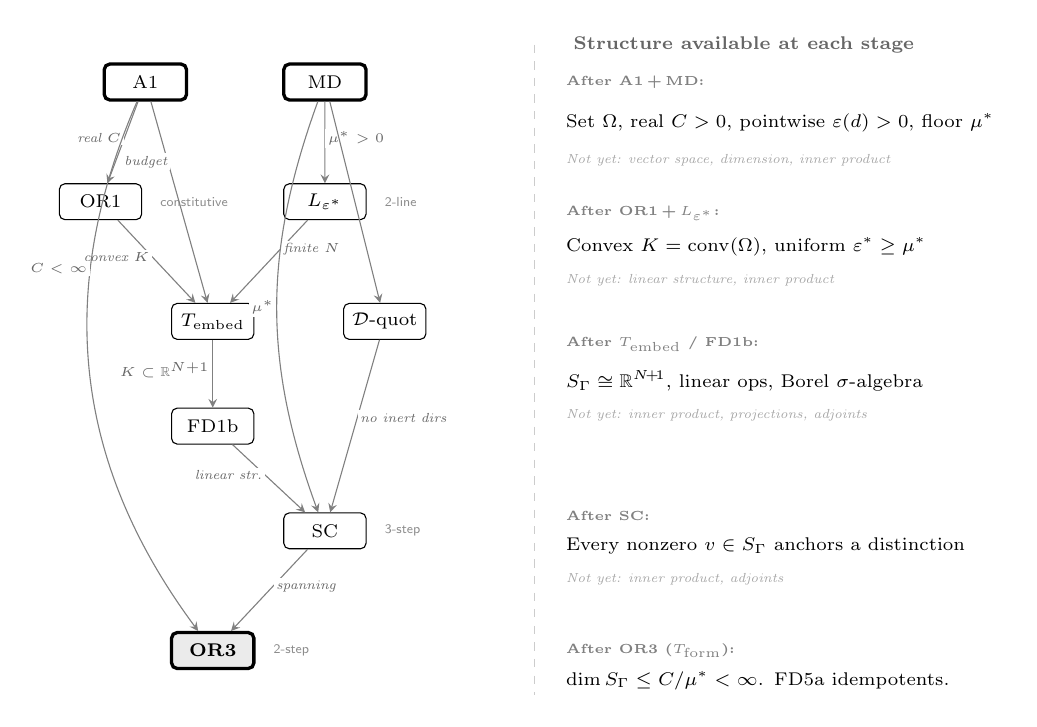
\begin{tikzpicture}[
    scale=0.95, every node/.style={transform shape},
    nd/.style={draw, rounded corners=2pt, minimum height=0.48cm, minimum width=1.1cm, inner sep=2pt, font=\scriptsize},
    input/.style={nd, very thick},
    derived/.style={nd},
    target/.style={nd, fill=black!8, very thick},
    arr/.style={->, >=stealth, thin, black!50},
    elabel/.style={font=\tiny\itshape, text=black!60, fill=white, inner sep=1pt},
    badge/.style={font=\tiny, text=black!45, anchor=west},
    inventory/.style={font=\scriptsize, anchor=west, text width=5.8cm, align=left},
    invlabel/.style={font=\tiny\bfseries, anchor=west, text=black!50},
    noyet/.style={font=\tiny\itshape, text=black!35, anchor=west},
]

% ── Nodes (left half) ──
\node[input] (A1) at (0, 0) {A1};
\node[input] (MD) at (2.4, 0) {MD};

\node[derived] (OR1) at (-0.6, -1.6) {OR1};
\node[derived] (Leps) at (2.4, -1.6) {$L_{\varepsilon^*}$};

\node[derived] (Temb) at (0.9, -3.2) {$T_{\mathrm{embed}}$};
\node[derived] (FD1b) at (0.9, -4.6) {FD1b};

\node[derived] (Dquot) at (3.2, -3.2) {$\mathcal{D}$-quot};
\node[derived] (SC) at (2.4, -6.0) {SC};

\node[target] (OR3) at (0.9, -7.6) {\textbf{OR3}};

% ── Proof-type badges ──
\node[badge] at ($(OR1.east)+(0.12,0)$) {\textsf{constitutive}};
\node[badge] at ($(Leps.east)+(0.12,0)$) {\textsf{2-line}};
\node[badge] at ($(SC.east)+(0.12,0)$) {\textsf{3-step}};
\node[badge] at ($(OR3.east)+(0.12,0)$) {\textsf{2-step}};

% ── Arrows with edge labels ──
\draw[arr] (A1) -- node[elabel, left, pos=0.45] {real $C$} (OR1);
\draw[arr] (MD) -- node[elabel, right, pos=0.45] {$\mu^* > 0$} (Leps);
\draw[arr] (OR1) -- node[elabel, left, pos=0.45] {convex $K$} (Temb);
\draw[arr] (Leps) -- node[elabel, right, pos=0.35] {finite $N$} (Temb);
\draw[arr] (A1) -- node[elabel, left=-1pt, pos=0.3] {budget} (Temb);
\draw[arr] (Temb) -- node[elabel, left, pos=0.45] {$K \subset \mathbb{R}^{N+1}$} (FD1b);
\draw[arr] (MD) -- (Dquot);
\draw[arr] (FD1b) -- node[elabel, left, pos=0.45] {linear str.} (SC);
\draw[arr] (Dquot) -- node[elabel, right, pos=0.45] {no inert dirs} (SC);
\draw[arr] (MD) to[bend right=20] node[elabel, left, pos=0.5] {$\mu^*$} (SC);
\draw[arr] (A1) to[bend right=30] node[elabel, left, pos=0.3] {$C < \infty$} (OR3);
\draw[arr] (SC) -- node[elabel, right, pos=0.45] {spanning} (OR3);

% ── Structure inventory (right panel) ──
\draw[black!20, dashed] (5.2, 0.5) -- (5.2, -8.2);
\node[font=\scriptsize\bfseries, text=black!60] at (8.0, 0.5) {Structure available at each stage};

\node[invlabel] at (5.5, -0.0) {After A1\,+\,MD:};
\node[inventory] at (5.5, -0.55) {Set $\Omega$, real $C > 0$, pointwise $\varepsilon(d) > 0$, floor $\mu^*$};
\node[noyet] at (5.5, -1.05) {Not yet: vector space, dimension, inner product};

\node[invlabel] at (5.5, -1.75) {After OR1\,+\,$L_{\varepsilon^*}$:};
\node[inventory] at (5.5, -2.2) {Convex $K = \mathrm{conv}(\Omega)$, uniform $\varepsilon^* \ge \mu^*$};
\node[noyet] at (5.5, -2.65) {Not yet: linear structure, inner product};

\node[invlabel] at (5.5, -3.5) {After $T_{\mathrm{embed}}$ / FD1b:};
\node[inventory] at (5.5, -4.0) {$S_\Gamma \cong \mathbb{R}^{N\!+\!1}$, linear ops, Borel $\sigma$-algebra};
\node[noyet] at (5.5, -4.45) {Not yet: inner product, projections, adjoints};

\node[invlabel] at (5.5, -5.8) {After SC:};
\node[inventory] at (5.5, -6.2) {Every nonzero $v \in S_\Gamma$ anchors a distinction};
\node[noyet] at (5.5, -6.65) {Not yet: inner product, adjoints};

\node[invlabel] at (5.5, -7.6) {After OR3 ($T_{\mathrm{form}}$):};
\node[inventory] at (5.5, -8.0) {$\dim S_\Gamma \le C/\mu^* < \infty$.  FD5a idempotents.};

\end{tikzpicture}
\caption[Arena chain]{%
\textbf{Arena chain: from finite budget to finite-dimensional substrate.}
Each arrow is labelled with the structure it provides.
Right panel: the running inventory of available mathematical structure at each stage.
Inner products, orthogonal projections, and adjoints appear \emph{nowhere} in this chain;
they enter only at $T_{\mathrm{adj}}$ (Figure~\ref{fig:bridge_dag}).
}
\label{fig:arena_dag}
\end{figure}
\smallskip\noindent\textbf{Theorem OR3 (Finite Substrate).}  The enforcement substrate $S_\Gamma$ is finite-dimensional:
\[
\dim(S_\Gamma) \;<\; \infty.
\]

\textit{Status.}  OR3 is a \emph{theorem} (proved below as $T_{\mathrm{form}}$ from A1 + MD + SC), not a bare assumption.  It is the single structural result beyond A1 required for the core quantum derivation.


\begin{tcolorbox}[apfbox, title={Proposition SC (Substrate Completeness)}]
\label{prop:SC}
\textit{Every nonzero direction in the substrate is physically real: it anchors a distinction with positive enforcement cost.}

\smallskip\noindent\textbf{Statement.}  Let $\Gamma = (S_\Gamma, C(\Gamma))$ be an interface with vector-space structure (FD1b).  Then $S_\Gamma$ is spanned by anchor sets of irreducible distinctions: for every nonzero $v \in S_\Gamma$, there exists $d_v \in \mathcal{D}(\Gamma)$ with $M_{d_v} = \mathrm{span}\{v\}$ and $\varepsilon(d_v) > 0$.

\smallskip\noindent\textbf{Depends on.}  MD ($\varepsilon(d) \ge \mu^* \cdot n(d)$), $\mathcal{D}$-quotient (Proposition~\ref{prop:D_quotient_forced}), FD1b (vector-space structure).  Finite dimensionality (OR3) is \emph{not required}: the proof works for any vector space.

\smallskip\noindent\textbf{Status.}  \textbf{[Proved]} --- three-step proof.  Essential for avoiding circularity: SC feeds into $T_{\mathrm{form}}$ (OR3), not the reverse.

\smallskip\noindent\textbf{Downstream.}  Used in: $T_{\mathrm{form}}$ (finite dimensionality), $L_\Delta$ (existence of $d_\Gamma$), $L_\Pi$ (non-deactivation).

\smallskip\noindent\textbf{Proof.}

\textit{Step 1 (Every direction has positive enforcement cost).}  Let $v \in S_\Gamma$, $v \ne 0$.  Choose any linear functional $f \in S_\Gamma^*$ with $f(v) \ne 0$ (exists for any nonzero vector in any vector space).  Define the binary predicate $d_v: S_\Gamma \to \{0,1\}$ by $d_v(\sigma) = 1$ iff $f(\sigma) \ne 0$ --- equivalently, $d_v$ is the indicator of $S_\Gamma \setminus \ker(f)$.  This predicate is non-trivial ($v \notin \ker(f)$ and $\ker(f) \ne \emptyset$), Borel-measurable (the complement of a hyperplane), and has anchor set $M_{d_v} = \mathrm{span}\{v\}$ (the one-dimensional subspace is the minimal subspace on which $d_v$ depends, since $d_v$ detects precisely the $v$-direction component).  Its enforcement complexity is $n(d_v) = 1$ (one binary test determines whether the $v$-component is present).  By MD: $\varepsilon(d_v) \ge \mu^* \cdot n(d_v) = \mu^* > 0$.  Therefore $d_v \in \mathcal{D}(\Gamma)$.

\textit{Step 2 (No enforcement-inert directions).}  Suppose for contradiction that $\varepsilon(d_v) = 0$ for some nonzero $v$.  Then the $v$-component of $\sigma$ can be changed at zero cost.  By the $\mathcal{D}$-quotient (Proposition~\ref{prop:D_quotient_forced}, Part~1): a degree of freedom that can be changed at zero cost is operationally inert and does not belong to $S_\Gamma$.  But $v \in S_\Gamma$ by hypothesis.  Contradiction.

\textit{Step 3 (Spanning).}  Since every nonzero $v \in S_\Gamma$ anchors a distinction $d_v \in \mathcal{D}$ with $M_{d_v} = \mathrm{span}\{v\}$, the anchor sets of irreducible distinctions span $S_\Gamma$: $\mathrm{span}\{M_{d_v} : v \in S_\Gamma \setminus \{0\}\} = S_\Gamma$.  \hfill$\square$

\smallskip\noindent\textit{Status.}  SC is a theorem of MD + $\mathcal{D}$-quotient + FD1b (all established before SC is invoked).  It is not an independent condition.  Crucially, SC does not assume OR3 ($\dim S_\Gamma < \infty$); it holds for any vector space $S_\Gamma$, finite- or infinite-dimensional.  This is essential for avoiding circularity, since OR3 is proved \emph{from} SC in $T_{\mathrm{form}}$ below.

\coderef{check\_SC}{paper1.py}\,%
\hspace{1em}\textit{(also verified in \texttt{supplement.py})}
\end{tcolorbox}

\smallskip\noindent\textit{Remark (uncountability of $\mathcal{D}(\Gamma)$ and why it is harmless).}  $\mathcal{D}(\Gamma)$ comprises \emph{all} Borel-measurable binary predicates $d: S_\Gamma \to \{0,1\}$ with $\varepsilon(d) > 0$.  Even when $\dim S_\Gamma = n < \infty$, this set is uncountably infinite: the set of one-dimensional subspaces of $\mathbb{R}^n$ is the real projective space $\mathbb{RP}^{n-1}$ (uncountable for $n \ge 2$), and each subspace supports uncountably many non-trivial Borel partitions.  None of the results in this paper require $|\mathcal{D}(\Gamma)|$ to be finite or countable, for the following reasons.  (i)~The minimum-cost floor $\varepsilon^* \ge \mu^* > 0$ (proved in $L_{\varepsilon^*}$) follows from MD applied element-wise: $\varepsilon(d) \ge \mu^* \cdot n(d) \ge \mu^*$ for each $d \in \mathcal{D}$ (since $n(d) \ge 1$), with no cardinality assumption.  (ii)~Every finiteness bound in the paper is a bound on the number of \emph{simultaneously active, independently enforceable} distinctions at a given interface --- i.e., on $|S_\sigma|$ where $S_\sigma \in \mathcal{D}_{\mathrm{ind}}(\Gamma)$ --- not on $|\mathcal{D}(\Gamma)|$.  The cost bound $|S_\sigma| \le \lfloor C/\varepsilon^* \rfloor$ gives the finite active-set count.  (iii)~The $T_{\mathrm{form}}$ proof below bounds $\dim(S_\Gamma)$ by bounding the total dimension cost of any independently enforceable subset via MD and A1's budget constraint.  The uncountable ambient set $\mathcal{D}(\Gamma)$ plays no role in the bound.

\smallskip\noindent\textbf{Proof of $T_{\mathrm{form}}$ (OR3 from A1 + MD + SC).}

\noindent\textit{Staging note.}  This proof uses the post-OR1 linear structure of $S_\Gamma$: OR1 (convex mixing) and $L_{\varepsilon^*}$ together give the canonical embedding $\varphi: \Omega \hookrightarrow \mathbb{R}^{N+1}$ with $N \le \lfloor C/\varepsilon^* \rfloor$ (formalized as $T_{\mathrm{embed}}$ below).  The embedding provides the linear-independence and dimension concepts used in Steps~1--2.  The post-geometric form $n(d) = \dim(M_d)$ applies throughout this proof.

\textit{Step 1 (Budget bound on independently enforceable sets).}  Let $\mathcal{I} \subseteq \mathcal{D}(\Gamma)$ be any pairwise independently enforceable set ($M_d \cap M_{d'} = \{0\}$ for all $d \neq d' \in \mathcal{I}$).  By MD, $\varepsilon(d) \ge \mu^* \cdot \dim(M_d)$ for each $d \in \mathcal{I}$.  Summing over the set and applying the budget constraint (A1):
\[
\sum_{d \in \mathcal{I}} \dim(M_d) \;\leq\; \frac{1}{\mu^*}\sum_{d \in \mathcal{I}} \varepsilon(d) \;\leq\; \frac{C(\Gamma)}{\mu^*} \;<\; \infty.
\]
\noindent\textit{Note.}  This bound does not require the sum of anchor sets to be direct; it follows from MD and A1 alone, applied term-by-term.

\textit{Step 2 (No linearly independent set exceeds $C/\mu^*$ in size).}  Let $\{v_1, \ldots, v_k\} \subseteq S_\Gamma$ be any finite linearly independent set (no finiteness of $S_\Gamma$ is assumed).  By SC, each $v_i$ anchors an irreducible distinction $d_{v_i} \in \mathcal{D}$ with $M_{d_{v_i}} = \mathrm{span}\{v_i\}$.  Since $\{v_i\}$ are linearly independent, $M_{d_{v_i}} \cap M_{d_{v_j}} = \{0\}$ for $i \ne j$, so $\{d_{v_1}, \ldots, d_{v_k}\}$ is pairwise independently enforceable.  By Step~1:
\[
k \;\leq\; \sum_{i=1}^k \dim(M_{d_{v_i}}) \;\leq\; \frac{C(\Gamma)}{\mu^*} \;<\; \infty.
\]
Since $k$ was an arbitrary finite linearly independent set size, no linearly independent subset of $S_\Gamma$ can have more than $\lfloor C(\Gamma)/\mu^* \rfloor$ elements.  Therefore:
\[
\dim(S_\Gamma) \;\leq\; \frac{C(\Gamma)}{\mu^*} \;<\; \infty. \qquad \square
\]

\textit{Empirical content: zero.}  OR3's role is to make the mathematical structure well-defined; it generates no independently falsifiable prediction.  Paper~6 confirms OR3 independently from the Bekenstein--Hawking bound~\cite{Bekenstein1981}: any finite region with area $A$ supports at most $A/4\ell_P^2 < \infty$ independent degrees of freedom.

\smallskip\noindent\textit{Relationship to QFT's infinite-dimensional local algebras.}  Quantum field theory assigns an infinite-dimensional von Neumann algebra $\mathcal{R}(\mathcal{O})$ to each bounded spacetime region $\mathcal{O}$.  OR3 ($\dim S_\Gamma < \infty$) appears to conflict with this.  The resolution is that OR3 is a statement about \emph{finite-capacity} interfaces: $\dim S_\Gamma \le C(\Gamma)/\mu^* < \infty$ holds at any finite budget $C(\Gamma)$.  QFT's infinite-dimensional algebras correspond to the continuum limit $C \to \infty$ (equivalently $\varepsilon^* \to 0$), in which the number of independently enforceable distinctions $n_{\max} = \lfloor C/\varepsilon^* \rfloor \to \infty$ and the algebra becomes infinite-dimensional.  The finite-$C$ theory is an effective description at finite resolution, analogous to the relationship between a lattice gauge theory at finite lattice spacing and its continuum limit.  Operationally: any experiment with finite energy, finite volume, and finite measurement precision accesses only finitely many independent degrees of freedom, so OR3 is satisfied in every realizable operational fragment.  The Bekenstein--Hawking bound (Paper~6) confirms that nature itself respects OR3 for bounded regions: any region enclosed by area $A$ has $n_{\max} \le A/4\ell_P^2$, which is enormous ($\sim 10^{69}$ for a $1\,\mathrm{m}^2$ boundary) but finite.  The APF does not replace QFT's infinite-dimensional algebras; it identifies them as the $C \to \infty$ idealization of an underlying finite-capacity structure.

\smallskip\noindent\textit{Concrete accommodation of continuous-variable systems.}  A quantum harmonic oscillator has infinitely many energy levels $E_n = (n + \tfrac{1}{2})\hbar\omega$, so its full Fock space is infinite-dimensional.  In the APF, a harmonic oscillator at a finite-capacity interface $\Gamma$ with budget $C(\Gamma)$ supports at most $n_{\max} = \lfloor C(\Gamma)/\varepsilon^*\rfloor$ independently enforceable distinctions.  Identifying $\varepsilon^*$ with the energy quantum $\hbar\omega$ (via $L_{\mathrm{cost}}$: enforcement cost proportional to energy gap), this is $n_{\max} = \lfloor C/\hbar\omega \rfloor$: the number of resolvable energy levels at finite capacity.  The full Fock space $\ell^2(\mathbb{N})$ is recovered in the limit $C/\hbar\omega \to \infty$.  At any finite $C$, the oscillator has a finite-dimensional enforcement algebra $M_{n_{\max}}(\mathbb{C})$; at $C = \infty$, the algebra becomes $B(\ell^2(\mathbb{N}))$ and OR3 no longer applies.  No APF result claims finiteness at infinite capacity.

The same mechanism handles quantum fields.  A free scalar field in a box of volume $V$ has mode frequencies $\omega_k = c|k|$ with $k$ discretized by the box boundary.  At finite capacity $C$, modes with $\hbar\omega_k > C$ are not enforceable (their single-distinction cost exceeds the total budget); only the $N_{\mathrm{modes}} \le \lfloor C/\hbar\omega_{\min}\rfloor$ lowest modes participate.  The APF algebra at finite $C$ is the tensor product of finitely many finite-dimensional matrix algebras --- one per enforceable mode --- which is finite-dimensional.  The continuum QFT ($V \to \infty$, $C \to \infty$) recovers the infinite tensor product of infinite-dimensional Fock spaces.  Lattice regularization in QFT achieves the same finite-dimensional truncation by a different route (discretizing space rather than capping the budget); the APF's route is budget-based rather than geometry-based but produces the same finite-dimensional effective theory at any finite cutoff.

\begin{tcolorbox}[apfbox, title={Theorem $T_{\mathrm{embed}}$ (Canonical Embedding): FD1a $\to$ FD1b}]
\label{thm:T_embed}
\textit{The abstract state set $\Omega$ embeds into a finite-dimensional real vector space, giving the substrate its linear structure.}

\smallskip\noindent\textbf{Statement.}  Let $\Gamma$ be an interface in the sense of FD1a.  Assume OR1 (convex mixing) and $\varepsilon^* > 0$ (from MD via $L_{\varepsilon^*}$).  Then:
\begin{enumerate}[nosep,leftmargin=2em,itemsep=2pt,label=(\alph*)]
\item There exists an injection $\varphi: \Omega(\Gamma)/{\sim_\mathcal{D}} \;\hookrightarrow\; \mathbb{R}^{N+1}$ with $N \leq \lfloor C/\varepsilon^* \rfloor < \infty$.
\item $\varphi$ preserves the cost functional: $\varphi(\sigma)_b = \varepsilon(b)\,\mathbf{1}_{b \in S_\sigma}$ for each $b \in \mathcal{B}$, and $\varphi(\sigma)_{N+1} = \delta_\sigma$.
\item The convex hull $K := \mathrm{conv}(\varphi(\Omega))$ is a compact convex set in a finite-dimensional real vector space $V = \mathrm{span}_\mathbb{R}(K) \subseteq \mathbb{R}^{N+1}$.
\end{enumerate}

\smallskip\noindent\textbf{Depends on.}  A1 (finite budget), OR1 (convex mixing; derived from real-valued $C$), $L_{\varepsilon^*}$ ($\varepsilon^* > 0$; from MD).

\smallskip\noindent\textbf{Status.}  \textbf{[Proved]} --- constructive: the embedding $\varphi$ is explicitly defined; injectivity, cost preservation, and compactness each verified.

\smallskip\noindent\textbf{Downstream.}  Establishes FD1b (vector-space structure on $S_\Gamma$), which all subsequent definitions (FD3--FD6) and the arena chain (Figure~\ref{fig:arena_dag}) require.

\smallskip\noindent\textbf{Proof.}

\textit{Construction.}  Let $\mathcal{B} \subseteq \mathcal{D}(\Gamma)$ be any maximal pairwise independently enforceable set (maximal antichain under $d \perp d'$; exists by Zorn's lemma).  $\mathcal{B}$ is finite: each $b \in \mathcal{B}$ costs $\varepsilon(b) \ge \varepsilon^* > 0$ ($L_{\varepsilon^*}$), these costs sum to at most $C(\Gamma)$ (A1), so $N := |\mathcal{B}| \leq \lfloor C(\Gamma)/\varepsilon^* \rfloor < \infty$.  (This finiteness argument is self-contained: it uses only $L_{\varepsilon^*}$ and A1, not $T_{\mathrm{form}}$.)  Define
\[
\varphi: \Omega(\Gamma) \;\longrightarrow\; \mathbb{R}^{N+1}, \qquad \varphi(S,\delta) \;=\; \bigl(\varepsilon(b)\,\mathbf{1}_{b \in S}\bigr)_{b \in \mathcal{B}} \;\oplus\; \delta.
\]

\textit{(a) Injectivity on $\mathcal{D}$-equivalence classes.}  Let $\sigma_1 = (S_1, \delta_1)$ and $\sigma_2 = (S_2, \delta_2)$ with $\varphi(\sigma_1) = \varphi(\sigma_2)$.  Then $\varepsilon(b)\,\mathbf{1}_{b \in S_1} = \varepsilon(b)\,\mathbf{1}_{b \in S_2}$ for every $b \in \mathcal{B}$; since $\varepsilon(b) > 0$, this gives $\mathbf{1}_{b \in S_1} = \mathbf{1}_{b \in S_2}$, so $S_1 \cap \mathcal{B} = S_2 \cap \mathcal{B}$.  The last component gives $\delta_1 = \delta_2$.  By the maximality of $\mathcal{B}$: any distinction $d \in S_1 \setminus \mathcal{B}$ has $M_d \subseteq \bigoplus_{b \in \mathcal{B}} M_b$ (otherwise $\mathcal{B} \cup \{d\}$ would be a larger antichain, contradicting maximality).  Its activation status is therefore determined by the $\mathcal{B}$-components and the residual $\delta$, which agree.  So $\sigma_1 \sim_\mathcal{D} \sigma_2$: the two states are $\mathcal{D}$-equivalent.  Therefore $\varphi$ is injective on equivalence classes.  \hfill$\square_a$

\textit{(b) Cost preservation.}  Immediate from the construction: the $b$-component of $\varphi(\sigma)$ is $\varepsilon(b)$ when $b$ is active and $0$ otherwise; the last component is the residual budget $\delta_\sigma = C - \sum_{b \in S_\sigma} \varepsilon(b)$.  The full cost information is encoded.  \hfill$\square_b$

\textit{(c) Compact convex hull.}  By OR1 (convex mixing), any convex combination $\lambda\sigma_1 + (1{-}\lambda)\sigma_2$ of admissible states is admissible (the budget integral is linear in the mixing parameter).  Therefore $K = \mathrm{conv}(\varphi(\Omega))$ is convex.  For compactness: $\varphi(\Omega) \subseteq [0, C]^{N+1}$ (each coordinate is bounded by the budget), so $\varphi(\Omega)$ is a bounded subset of $\mathbb{R}^{N+1}$; and $\Omega$ is a finite union of finitely many activation patterns (at most $2^N$ subsets of $\mathcal{B}$), each a point in $\mathbb{R}^{N+1}$, so $\varphi(\Omega)$ is finite and hence closed.  The convex hull of a finite set of points in $\mathbb{R}^{N+1}$ is a compact convex polytope.  $V = \mathrm{span}_\mathbb{R}(K)$ has $\dim V \leq N + 1 < \infty$.  \hfill$\square_c$

\smallskip\noindent\textit{Status.}  $T_{\mathrm{embed}}$ provides the GPT state-space embedding.  The three conditions verified --- injectivity on $\mathcal{D}$-classes, cost preservation, compact convex hull in finite dimensions --- are the standard requirements (cf.\ Barnum--Wilce~\cite{BarnumWilce2012}, \S2).  After $T_{\mathrm{embed}}$, $S_\Gamma$ is a finite-dimensional real vector space (FD1b) and all subsequent definitions (FD3, FD4, FD5, FD6) apply.

\coderef{check\_T\_embed}{paper1.py}
\end{tcolorbox}
\begin{tcolorbox}[defbox, title={$\mathrm{FD4b}$ (Definition: Admissible Perturbation)}]

\noindent\textbf{Definition.}  A \emph{perturbation} $p$ of distinction $d$ at interface $\Gamma$ is any element of $\mathrm{End}(S_\Gamma)$ satisfying:
\begin{enumerate}[nosep,leftmargin=2em,itemsep=3pt,label=(\roman*)]
  \item \textbf{Realizability.}  $p$ is a physically realizable operation on the enforcement substrate $S_\Gamma$: an element of a well-defined perturbation set $\mathcal{P}_{\mathrm{all}} \subseteq \mathrm{End}(S_\Gamma)$ closed under composition.
  \item \textbf{Positive cost.}  $\mathrm{cost}(p) > 0$.  (Zero-cost perturbations would imply $\varepsilon(d) = 0$, contradicting membership in $\mathcal{D}$.)
  \item \textbf{Destructive effect.}  $p$ reduces the enforcement level of $d$ below $\varepsilon(d)$; equivalently, after $p$ acts, $d$ can no longer be certified as active given the remaining budget.
  \item \textbf{Cost subadditivity.}  For any $p_1, p_2 \in \mathcal{P}_{\mathrm{all}}$: $\mathrm{cost}(p_1 \cdot p_2) \le \mathrm{cost}(p_1) + \mathrm{cost}(p_2)$.  This is a consequence of A1, not a separate assumption: perturbations consume enforcement capacity from the same finite pool that A1 constrains; sequential execution costs at most the sum; the composite achieves the same endpoint in one step and therefore cannot require more.
  \item \textbf{Localization type.}  $p$ belongs to exactly one of two formally separated classes:
    \begin{itemize}[nosep,leftmargin=2em,itemsep=1pt]
      \item $p \in \mathcal{P}(d)$: mechanism-localized ($\mathrm{supp}(p) \subseteq M_d$; this is tautological from FD3's definition of $M_d$); or
      \item $p \in \mathcal{P}_\Gamma$: substrate-targeting (acts on $S_\Gamma$ as a whole, reducing $C(\Gamma)$).
    \end{itemize}
    No perturbation belongs to both classes (formal separation).
\end{enumerate}

Clauses (i)--(iii) and (v) formalize the English meaning of ``a perturbation that can destroy a distinction at positive cost.''  Clause (iv) is derived from A1 (the attacker cannot generate resources from nothing).  The entire definition is therefore fixed by the semantics of A1 and the word ``perturbation''; no additional structural input enters.

\smallskip\noindent\textbf{Closure rule for joint perturbation sets.}
\[
\mathcal{P}(\{d_1,\ldots,d_k\}) \;:=\; \mathcal{P}(d_1) \cup \cdots \cup \mathcal{P}(d_k) \;\cup\; \mathcal{P}_\Gamma\bigl(\{d_1,\ldots,d_k\}\bigr),
\]
where $\mathcal{P}_\Gamma(\{d_1,\ldots,d_k\})$ is the set of substrate perturbations that simultaneously threaten all distinctions in the set (Lemma~P2).  By Lemma~P3, for any two co-located distinctions this union is \emph{strict}: $\mathcal{P}(\{d_1,d_2\}) \supsetneq \mathcal{P}(d_1) \cup \mathcal{P}(d_2)$.

\smallskip\noindent\textit{Physical verification.}  Appendix~F gives three worked physical systems (spin-$\tfrac{1}{2}$ in a thermal bath; classical 3-bit repetition code; Steane $[\![7,1,3]\!]$ stabilizer code) in which FD4b(i)--(v) are verified and maintenance, detection, and destruction costs are computed explicitly.
\end{tcolorbox}

\smallskip\noindent\textit{Perturbation lemmas P1--P4} (derived from A1 + $T_{\mathrm{sep}}$ + OR3; provide independent LP verification of $L_\Delta$) \textit{are in Section~\ref{sec:P1P4_detail}.  They are not on the critical path; the primary $L_\Delta$ proof uses the substrate-integrity argument directly.}

\subsection{Structural lemmas of the arena}
\label{sec:lemmas}

Before deriving the five lemmas, it is useful to consolidate what ``enforcement'' means.  The following box collects the three-layer architecture that the derivations below rely on:  Layer~1 is the physical axiom A1 and the structural assumption MD; Layer~2 is the definitions (FD1--FD5) of what enforcement is; Layer~3 is the derived mathematical structure.


\medskip\noindent\textit{Operational Semantics of Enforcement: Three-Layer Architecture.}
\textbf{Layer 1 --- Physical axiom (A1) and structural assumption (MD).}  A1: enforcement capacity is finite and positive: $0 < C(\Gamma) < \infty$ for every interface $\Gamma$, and $\sum_{d \in \mathcal{D}(\sigma,\Gamma)} \varepsilon(d) \le C(\Gamma)$ for every admissible state $\sigma$.  MD: enforcement cost is bounded below by enforcement complexity: $\varepsilon(d) \ge \mu^* \cdot n(d)$, where $n(d) \ge 1$ is the minimum binary tests to specify $d$'s status (equivalently $\varepsilon(d) \ge \mu^* \cdot \dim(M_d)$ after FD1b; Section~\ref{assumption:MD}).  Together, A1 and MD supply the budget bound, positivity, and the uniform cost floor $\varepsilon^* > 0$.

\medskip\noindent\textbf{Layer 2 --- Operational semantics of enforcement.}  The following are definitional, not physical:
\begin{enumerate}[nosep,leftmargin=2em,itemsep=3pt,label=(\roman*)]
  \item \textit{Enforcement strategies are budget-allocation maps.}  An enforcement strategy at $\Gamma$ is a map from the budget pool $C(\Gamma) \in \mathbb{R}_{>0}$ to the set of simultaneously maintained distinctions, subject to the admissibility constraint.  A1 constrains how much budget is available; the semantics of what ``allocating budget to $d$'' means is given by the definitions FD1--FD5.
  \item \textit{Each interface $\Gamma$ is physically instantiated by a substrate $S_\Gamma$} that carries its capacity $C(\Gamma)$ exclusively.  No degree of freedom belongs to two distinct interfaces (interface partition, $T_{\mathrm{cap}}$).  The substrate $S_\Gamma$ provides the physical arena in which the enforcement operations $E_d = \pi_{M_d}$ act.
  \item \textit{Perturbation classes are formally separated.}  $\mathcal{P}(d)$ contains perturbations that act only within $M_d$ and can destroy $d$.  $\mathcal{P}_\Gamma$ contains perturbations that act on the substrate pool $S_\Gamma \setminus \bigcup_d M_d$, degrading capacity without targeting any individual $d$.  This separation is the definitional content of ``independently enforceable'': FD4 then specifies the resource-competition relationship between attack and defense costs.
  \item \textit{OR0 (Faithfulness) is a consequence of A1.}  Two enforcement configurations that produce identical residual enforceability structures (same active distinctions, same residual budget $\delta_\sigma$) are the same physical state.  This follows from the $\mathcal{D}$-quotient structure of $\Omega$ (Proposition~\ref{prop:D_quotient_forced}): configurations that agree on all positive-cost distinctions are operationally indistinguishable within the enforcement framework and are therefore identified.
\end{enumerate}

\medskip\noindent\textbf{Layer 3 --- Derived structure.}  Everything else is a theorem: OR1 (convex mixing), OR2 (self-adjointness, $T_{\mathrm{adj}}$), OR3 (finite substrate, $T_{\mathrm{form}}$ from A1 + MD + SC), Cost Discreteness, the five structural lemmas, and all quantum structure T1--T2.  FD1b (vector-space substrate) is derived from OR1 + $L_{\varepsilon^*}$ (Proposition~\ref{prop:FD1_derived}); FD4 is constitutive (Proposition~\ref{prop:FD4_constitutive}); FD6 is derived from $L_\Delta$ (Theorem~$L_{\mathrm{blk}}$ establishes failure of direct-sum realizability; Lemma~$L_\Pi$ provides the geometric construction of the joint defense codespace $W$).  The complete assumption inventory is in Section~\ref{sec:assumption_inventory}.

\medskip\noindent\textbf{Why this matters.}  The derivation chain below is only as strong as the layer separation is clean.  Every time the proofs below invoke ``by A1,'' they are using Layer~1 exclusively.  Every time they invoke a definition from FD1--FD5, they are using Layer~2.  The definitions in Layer~2 are now either constitutive (FD4: the unique formalization of enforcement cost given FD1--FD3; Proposition~\ref{prop:FD4_constitutive}) or derived (FD1: vector-space structure from real-valued budget; Proposition~\ref{prop:FD1_derived}).  FD6 is derived in Section~\ref{sec:formal_bridge} from $L_\Delta$ via Theorem~$L_{\mathrm{blk}}$ and Lemma~$L_\Pi$.  The only structural assumption beyond A1 is MD (Layer~1.5: structural assumption, Section~\ref{sec:assumption_inventory}).  The mathematical content emerges from the interaction between Layer~1's finiteness and Layer~2's constitutive definitions.

\subsection{\texorpdfstring{$L_{\varepsilon^*}$}{L epsilon*} (Minimum Cost): no infinitesimal distinctions}
\label{sec:eps_star}

If distinctions could be maintained at arbitrarily small cost, an unbounded number of them could fit within any finite capacity---and finiteness would carry no structural force.  The route to blocking this starts with the no-Zeno content of A1 (Aspect~3, Section~\ref{sec:axiom}).

\medskip\noindent\textbf{Definition (Enforcement history).}
An \emph{enforcement history} on region $R$ is a finite sequence of capacity commitments whose cumulative effect maintains a set of distinctions in an admissible state.  An enforcement history is \emph{physically realizable} if it can be executed as a finite commitment process within the available budget of $R$.

\begin{tcolorbox}[apfbox, title={Lemma $L_{\mathrm{NZ}}$ (No Zeno Enforcement)}]
\textit{Enforcement histories cannot contain infinitely many ever-smaller commitment acts --- enforcement terminates.}

\smallskip\noindent\textbf{Statement.}  No physically realizable enforcement history on a region $R$ with $C(R) < \infty$ contains an infinite strictly descending sequence of positive commitment costs
\[
\varepsilon_1 > \varepsilon_2 > \varepsilon_3 > \cdots > 0, \qquad \varepsilon_n \to 0,
\]
all of which are required as distinct nonzero enforcement acts in a single admissible realization.

\smallskip\noindent\textbf{Depends on.}  A1 (Aspect 3: enforcement is a realizable commitment process, not a formal limit).

\smallskip\noindent\textbf{Status.}  \textbf{[Proved]} from A1's operational content.  Does \emph{not} establish $\varepsilon^* > 0$ (that requires MD via $L_{\varepsilon^*}$).

\smallskip\noindent\textbf{Proof.}
This is a corollary of A1's operational content (Aspect~3).  An enforcement history is physically realizable only if it terminates as a finite commitment process.  If a history required an infinite strictly descending sequence of distinct positive enforcement acts with costs approaching zero, then its realization would depend on arbitrarily fine subdivisions of the enforcement process --- it would have no terminal enforcement scale and could never complete as a physical act.  Enforcement is not a formal limit of ever-finer approximations; it is a realized commitment.  A1 treats maintained distinctions as physically realized commitments within a finite budget, not as limits of infinitely refinable procedures.  Therefore admissible enforcement histories exclude Zeno sequences.  \hfill$\square$

\smallskip\noindent\textit{Remark.}  $L_{\mathrm{NZ}}$ does not follow from the budget inequality alone.  The series $\sum_{n=1}^\infty 2^{-n} = 1$ shows that infinitely many positive commitments can sum to a finite budget.  What $L_{\mathrm{NZ}}$ uses is the physical realizability clause: enforcement acts must terminate.  This is the operational content of ``finite enforceability'' that $L_{\mathrm{NZ}}$ makes precise.

\smallskip\noindent\textit{Status.}  $L_{\mathrm{NZ}}$ is derived from A1's operational content (Aspect~3): physical realizability of enforcement excludes Zeno sequences within any single enforcement history.  What $L_{\mathrm{NZ}}$ establishes and what it does \emph{not} establish are both important.  It \emph{establishes} that no admissible history contains an infinite descending sequence of distinct positive enforcement acts.  It does \emph{not} establish that $\mathcal{D}$ cannot contain arbitrarily cheap distinct distinctions: a universe with $\mathcal{D} = \{d_n : \varepsilon(d_n) = 1/n\}$ would have every finite enforcement history Zeno-free while $\inf_{d \in \mathcal{D}} \varepsilon(d) = 0$.  One might attempt to bootstrap $\varepsilon^* > 0$ from $L_{\mathrm{NZ}}$ combined with $L_{\mathrm{loc}}$ (locality at a single interface); but $L_{\mathrm{loc}}$ bounds the history at a fixed interface and is itself proved after $L_{\varepsilon^*}$ in the dependency order --- using it here would introduce a circular dependency.  The uniform positive floor $\varepsilon^* > 0$ is proved via MD: $\varepsilon(d) \geq \mu^* \cdot n(d) \geq \mu^* > 0$ for every $d \in \mathcal{D}$, independent of $T_{\mathrm{sep}}$ (Section~\ref{sec:logical_status_eps_star}).

\coderef{check\_L\_NZ}{paper1.py}
\end{tcolorbox}

\begin{tcolorbox}[apfbox, title={$L_{\varepsilon^*}$ (Minimum Cost) --- Theorem}]
\label{sec:logical_status_eps_star}
\textit{No distinction can be maintained for free: there is a uniform positive floor on all enforcement costs.}

\smallskip\noindent\textbf{Statement.}  There exists $\varepsilon^* > 0$ such that every enforceable distinction costs at least $\varepsilon^*$:
\[
\varepsilon(d) \;\ge\; \varepsilon^* \;>\; 0 \qquad \forall\; d \in \mathcal{D}.
\]

\smallskip\noindent\textbf{\textit{Variables:}}
\begin{varlist}
\item $\varepsilon(d)$ --- enforcement cost of distinction $d$: the infimum perturbation cost to destroy $d$ (FD4).
\item $\varepsilon^* := \inf_{d \in \mathcal{D}} \varepsilon(d)$ --- the minimum enforcement cost across all distinctions.
\item $\mu^* > 0$ --- the per-test cost floor from MD.
\item $n(d) \ge 1$ --- enforcement complexity of $d$: minimum binary tests to specify $d$'s status (Section~\ref{assumption:MD}).
\end{varlist}

\smallskip\noindent\textbf{Depends on.}  MD only (enforcement isotropy: $\varepsilon(d) \ge \mu^* \cdot n(d)$ with $n(d) \ge 1$).

\smallskip\noindent\textbf{Status.}  \textbf{[Proved]} --- two-step proof from MD.  Does not require OR3, $T_{\mathrm{sep}}$, or any derived structure.

\smallskip\noindent\textbf{Downstream.}  Used in: $T_{\mathrm{embed}}$ (finite $N$ for canonical embedding), $T_{\mathrm{form}}$/OR3 ($\dim S_\Gamma < \infty$), $L_{\mathrm{cost}}$ (cost uniqueness), $L_{\mathrm{loc}}$ (budget additivity).

\smallskip\noindent\textbf{Why A1 alone does not suffice.}  A1 gives $C < \infty$ and pointwise $\varepsilon(d) > 0$ for each individual $d \in \mathcal{D}$.  But pointwise positivity on an infinite index set does not imply a uniform floor: the sequence $\varepsilon(d_n) = 1/n$ is a standard counterexample in which each cost is positive, yet $\inf_n \varepsilon(d_n) = 0$.  The uniform floor requires either a bound on $|\mathcal{D}|$ (unavailable: $\mathcal{D}$ may be uncountably infinite) or a $d$-independent lower bound on $\varepsilon(d)$.  MD supplies the latter directly.

\smallskip\noindent\textbf{Proof.}

\textit{Step~1} (Uniform lower bound from MD).  Let $d \in \mathcal{D}$ be arbitrary.  By assumption MD (pre-geometric form):
\[
\varepsilon(d) \;\geq\; \mu^* \cdot n(d),
\]
where $n(d) \ge 1$ is the enforcement complexity (minimum binary tests to specify $d$'s status; Section~\ref{assumption:MD}).  Since $d \in \mathcal{D}$ is a non-trivial binary predicate (FD2(i)), at least one binary test is needed to determine its enforcement status, so $n(d) \geq 1$.  Therefore $\varepsilon(d) \geq \mu^* \cdot 1 = \mu^* > 0$.  This holds for every $d \in \mathcal{D}$ with the same constant $\mu^* > 0$.  (After FD1b: $n(d) = \dim(M_d)$, recovering $\varepsilon(d) \ge \mu^* \cdot \dim(M_d)$.)

\textit{Step~2} (Infimum is attained positively).  Since $\varepsilon(d) \geq \mu^*$ for every $d \in \mathcal{D}$:
\[
\varepsilon^* \;:=\; \inf_{d \in \mathcal{D}} \varepsilon(d) \;\geq\; \mu^* \;>\; 0. \qquad \square
\]
No finiteness of $\mathcal{D}$ is invoked anywhere.

\smallskip\noindent\textbf{Consequence.}  The counting bound on \emph{simultaneously active, independently enforceable} distinctions follows.  For any admissible state $\sigma = (S_\sigma, \delta_\sigma) \in \Omega(\Gamma)$:
\[
|S_\sigma| \;\le\; \left\lfloor \frac{C(\Gamma)}{\varepsilon^*} \right\rfloor \;<\; \infty.
\]
Here $S_\sigma \in \mathcal{D}_{\mathrm{ind}}(\Gamma)$ is the independently enforceable active set (pairwise disjoint anchor sets), not the full universe $\mathcal{D}(\Gamma)$ of all Borel-measurable binary predicates with positive enforcement cost, which may be uncountably infinite (see the Remark below).

\smallskip\noindent\textit{Remark (from uncountable $\mathcal{D}$ to finite active sets).}  The universe of distinctions $\mathcal{D}(\Gamma)$ can be vast: even when $\dim S_\Gamma = n < \infty$, there are uncountably many one-dimensional subspaces of $\mathbb{R}^n$ (for $n \ge 2$), and for each subspace uncountably many Borel-measurable binary predicates that depend on it.  This uncountability is harmless, for two reasons that operate at different levels:

(i)~\emph{Per-distinction floor (MD).}  The proof above bounds $\varepsilon(d) \ge \mu^* > 0$ for \emph{every} $d \in \mathcal{D}(\Gamma)$, regardless of the cardinality of $\mathcal{D}$.  No finiteness or countability of $\mathcal{D}$ is invoked.

(ii)~\emph{Finite active-set bound (cost bound).}  Any admissible state activates only an independently enforceable set $S_\sigma$ with $\sum_{d \in S_\sigma} \varepsilon(d) \le C$.  Since each $\varepsilon(d) \ge \varepsilon^* > 0$ (part~(i)), at most $\lfloor C/\varepsilon^* \rfloor$ distinctions can be simultaneously active (Theorem D-fin, part~(c)).  Note: a purely geometric bound from pairwise $M_d \cap M_{d'} = \{0\}$ is tempting but invalid --- pairwise trivial intersection does not imply directness of the sum (see the remark after D-fin(c)).  The cost bound is the correct finiteness argument.

The collapse mechanism is: $\mathcal{D}(\Gamma)$ is uncountably infinite $\to$ the $\mathcal{D}$-quotient identifies distinctions with identical anchor geometry and cost $\to$ the independence requirement restricts any single state to pairwise-disjoint anchor sets $\to$ the cost bound $\sum \varepsilon(d) \le C$ with each $\varepsilon(d) \ge \varepsilon^*$ caps the active count at $\lfloor C/\varepsilon^* \rfloor$.  At no point does the argument require $|\mathcal{D}(\Gamma)|$ to be finite.

\smallskip\noindent\textit{Remark (role of OR3 and MD).}  The MD-direct proof above does not require $\mathcal{D}$ to be finite or even countable.  OR3's role in this paper is not to bound $|\mathcal{D}|$ but to supply $\dim(S_\Gamma) < \infty$, which is needed for the Wedderburn--Artin step in T2 and for the finite-dimensional representation theory throughout.  MD is the load-bearing assumption for $\varepsilon^* > 0$: it is A1 applied one level deeper, to substrate dimensions rather than object-level distinctions.

\smallskip\noindent\textit{Continuous-parameter systems and the cost floor.}  A potential objection: in a system with a tunable energy splitting (e.g., a qubit with adjustable $\omega_{01}$), the splitting can be driven toward zero continuously.  Does this violate $\varepsilon^* > 0$?  No, for a precise reason.  As $\omega_{01} \to 0$, the distinction ``the qubit is in $|0\rangle$ rather than $|1\rangle$'' becomes thermally fragile: thermal fluctuations at any $T > 0$ can flip it at negligible cost.  In the limit $\omega_{01} = 0$, no perturbation is needed to destroy the distinction --- it is no longer enforced.  By A1's membership condition ($d \in \mathcal{D} \Leftrightarrow \varepsilon(d) > 0$), the distinction exits $\mathcal{D}$ at $\varepsilon(d) = 0$.  MD's cost floor $\mu^*$ is not about the minimum splitting achievable in a given device's parameter range; it is about the minimum cost per degree of freedom for any distinction that is \emph{physically real} (robustly maintained against perturbation).  A near-degenerate level is not a robust distinction.  The floor $\varepsilon^* \ge \mu^* > 0$ is global (platform-independent) because it is a property of the enforcer's minimum resolution, not of any particular device's tuning range.  Concretely: $\mu^*$ sets the scale below which a binary fact ceases to be a physical distinction and becomes a bookkeeping label with no enforcement cost --- and therefore, by A1's constitutive identification, no physical reality.

\smallskip\noindent\textbf{Physical value and empirical weight.}  By $L_{\mathrm{cost}}$ (Section~\ref{sec:L_cost}), the unique cost functional under A1 is $C(E) = n(E) \cdot \varepsilon^*$, so $\varepsilon^*$ cancels from every dimensionless prediction.  Paper~6 confirms $\varepsilon^* = \alpha\ell_p^2$ from the Bekenstein--Hawking bound~\cite{Bekenstein1981}, providing SI conversion.

\coderef{check\_L\_epsilon\_star}{paper1.py}
\end{tcolorbox}

% ======================================================================
% L_cost: moved here from the skeleton section to resolve forward-reference
% from L_loc. L_cost depends only on A1 + MD + T_sep + FD2.
% ======================================================================

\subsection{\texorpdfstring{$L_{\mathrm{cost}}$}{L cost}: cost functional uniqueness}
\label{sec:L_cost}\label{sec:L_map}

The proved status of $L_{\varepsilon^*}$ raises a natural follow-on question: does any quantitative claim of the framework depend on the numerical value of $\varepsilon^*$?  The answer is no, and the reason is a theorem provable entirely within this paper.

The key observation is that all dependencies of the paper are on \emph{ratios} of enforcement costs, never on their absolute values.  Once the form of the cost functional is pinned down, $\varepsilon^*$ cancels from every dimensionless ratio.  Pinning that form requires only A1, $L_{\mathrm{loc}}$, $T_M$, and $L_{\varepsilon^*}$ — all proved above.


\medskip\noindent\textbf{Sub-lemma C1 (Ledger Completeness).}
\textbf{Statement.}  The enforcement cost $C(E)$ depends only on the number of independent active channels $n(E) \in \mathbb{N}$ in enforcement structure $E$: there exists $f: \mathbb{N} \to \mathbb{R}_{>0}$ such that $C(E) = f(n(E))$.

\smallskip\noindent\textbf{Derivation.}  The argument has two steps, drawing on two distinct premises.  \textit{Step (a) (Exhaustive ledger, from A1).}  By A1, the budget account is exhaustive: every unit of capacity is allocated to a specific enforcement channel.  Therefore $C(E) = \sum_{d \in E} \varepsilon(d)$, i.e., cost depends on \emph{which} channels are active.  \textit{Step (b) (Channel-identity independence, from MD).}  By MD (Enforcement Isotropy), the per-channel enforcement cost depends only on the enforcement complexity $n(d)$, not on the identity of $d$: all irreducible distinctions ($n(d) = 1$) cost $\varepsilon(d) \ge \mu^*$, with equality for irreducible distinctions at saturating interfaces (the regime where $L_{\mathrm{cost}}$ is applied).  Two structures with the same channel count therefore have the same ledger total, regardless of which particular channels are active.  Without MD, Step~(a) alone gives $C(E) = \sum_{d \in E} \varepsilon(d)$, which depends on channel identity; MD is what collapses the dependence to channel count.  Therefore $C(E) = f(n(E))$ for some $f: \mathbb{N} \to \mathbb{R}_{>0}$.



\medskip\noindent\textbf{Sub-lemma C1b (Integrality).}
\textbf{Statement.}  The channel count $n(E) \in \mathbb{N}$ for any enforcement structure $E$ derived from $\mathcal{D}$.

\smallskip\noindent\textbf{Derivation.}  Each distinction $d \in \mathcal{D}$ is a binary predicate (either active or not; FD3), so it contributes exactly 0 or 1 independent channels.  The total channel count is the cardinality $|S_\sigma|$ of the active set, which is a non-negative integer.



\medskip\noindent\textbf{Sub-lemma C2 (Additive Independence).}
\textbf{Statement.}  For independently enforceable structures $E_1, E_2$ (disjoint anchor sets, from $T_{\mathrm{sep}}$): $f(n_1 + n_2) = f(n_1) + f(n_2)$, where $n_i = n(E_i)$.

\smallskip\noindent\textbf{Derivation.}  By $T_{\mathrm{sep}}$, independently enforceable structures have disjoint anchor sets and hence disjoint defense problems.  The budget required to defend both is exactly the sum of the individual defense budgets: no shared substrate means no combined-attack premium ($\Delta = 0$ in this regime).  Therefore $C(E_1 \cup E_2) = C(E_1) + C(E_2)$, which is the additivity condition $f(n_1 + n_2) = f(n_1) + f(n_2)$ on $\mathbb{N}$.


\begin{tcolorbox}[apfbox, title={$L_{\mathrm{cost}}$: Cost Functional Form Uniqueness}]
\textit{The enforcement cost of any structure is an integer multiple of the minimum cost quantum --- forced by the Cauchy functional equation on $\mathbb{N}$.}

\smallskip\noindent\textbf{Statement.}  Given (i) Sub-lemma~C1 (Ledger Completeness: $C(E) = f(n(E))$, derived from A1 + MD), (ii) Sub-lemma~C1b (Integrality: $n(E) \in \mathbb{N}$, derived from the binary-predicate structure of $\mathcal{D}$), and (iii) Sub-lemma~C2 (Additive Independence: $f(n_1 + n_2) = f(n_1) + f(n_2)$, derived from $T_{\mathrm{sep}}$), the cost functional has the unique form
\[
C(E) \;=\; n(E)\cdot\varepsilon^*,
\]
where $n(E) \in \mathbb{N}$ is the number of independent enforcement channels in structure $E$ and $\varepsilon^* := f(1) > 0$ is the unit cost.

\smallskip\noindent\textbf{\textit{Variables:}}
\begin{varlist}
\item $C(E)$ --- the total enforcement cost of structure $E$ (a set of simultaneously maintained distinctions).
\item $n(E) \in \mathbb{N}$ --- the number of independent enforcement channels (independent binary tests) in $E$.
\item $\varepsilon^* := f(1) > 0$ --- the minimum enforcement cost: the cost of a single irreducible distinction (from MD via $L_{\varepsilon^*}$).
\item $f: \mathbb{N} \to \mathbb{R}_{>0}$ --- the cost-per-channel function, shown to be $f(n) = n\varepsilon^*$.
\end{varlist}

\smallskip\noindent\textbf{Depends on.}  A1 (finite budget), MD (Enforcement Isotropy; channel-identity independence in C1), $T_{\mathrm{sep}}$ (cost additivity for independent distinctions; \S\ref{sec:defs}), $L_{\varepsilon^*}$ ($\varepsilon^* > 0$; \S\ref{sec:logical_status_eps_star}), binary-predicate structure of $\mathcal{D}$ (FD2).

\smallskip\noindent\textbf{Status.}  \textbf{[Proved]} --- conditional on Sub-lemmas C1, C1b, C2 (C1 from A1 + MD; C1b and C2 from A1 + definitions).  The Cauchy equation on $\mathbb{N}$ has a unique solution by induction; no regularity condition is needed.

\smallskip\noindent\textbf{Downstream.}  Used in: Disjoint Partition Proposition (substrate exclusivity), $L_{\mathrm{loc}}$ (budget additivity), NT (non-degeneracy), Cost Discreteness Corollary.

\smallskip\noindent\textit{Proof.}  Sub-lemma C1 (ledger completeness) establishes that $C(E)$ depends only on the number of active channels $n(E) \in \mathbb{N}$, so $C(E) = f(n(E))$ for some function $f: \mathbb{N} \to \mathbb{R}_{>0}$.  Sub-lemma C2 (additive independence from $T_{\mathrm{sep}}$) gives the Cauchy equation $f(n_1 + n_2) = f(n_1) + f(n_2)$ for all $n_1, n_2 \in \mathbb{N}$.  On $\mathbb{N}$, this equation has the unique solution $f(n) = n\varepsilon^*$ where $\varepsilon^* := f(1) > 0$: by induction, $f(n) = f(1 + \cdots + 1) = n\,f(1)$ for every $n \ge 1$.

\smallskip\noindent\textit{Why no regularity condition is needed.}  On the domain $\mathbb{R}_{>0}$, the Cauchy equation $f(x+y) = f(x) + f(y)$ admits pathological (Hamel-basis) solutions unless one imposes at least one of: (R1)~monotonicity, (R2)~Lebesgue measurability, (R3)~boundedness on some interval $(a,b)$, or (R4)~continuity at a single point~\cite{Aczel1966}.  Each of R1--R4 implies the others for Cauchy solutions and forces $f(x) = cx$.  None of these conditions is needed here, because the domain of $f$ is $\mathbb{N}$, not $\mathbb{R}_{>0}$.  The natural numbers have a single additive generator ($1 \in \mathbb{N}$), so $f$ is determined by $f(1)$ alone via induction; the uncountable Hamel basis of $\mathbb{R}$ over $\mathbb{Q}$ that supports pathological solutions does not exist on $\mathbb{N}$.  Monotonicity ($f(n+1) = f(n) + \varepsilon^* > f(n)$) and boundedness on every finite interval are \emph{consequences}, not assumptions.  The integrality of $n(E)$ --- derived from the binary-predicate structure of $\mathcal{D}$ (Sub-lemma~C1b), not assumed --- is what restricts the domain to $\mathbb{N}$ and closes the argument unconditionally.  \hfill$\square$

\coderef{check\_L\_cost}{paper1.py}\,%
\hspace{1em}\textit{(also verified in \texttt{supplement.py})}
\end{tcolorbox}

\smallskip\noindent\textit{Physical-domain verification and scope.}  The abstract uniqueness theorem is verified in concrete physical domains immediately below: Section~\ref{sec:Lcost_worked} instantiates $L_{\mathrm{cost}}$ for QEC syndrome extraction overhead in the surface code, verifying V1--V3 from operational data and computing the conversion factor $\alpha_\gamma$.  Section~\ref{sec:dual_ruler} then provides the end-to-end dual-ruler verification: two independent physical proxies (energy gap and syndrome count) in the same system (Kitaev toric code), both satisfying V1--V3, both mapping to the same $\varepsilon(\cdot)$, with a parameter-free cross-ruler ratio --- using no companion-paper results.  The proxy table (Table~\ref{tab:physical_proxies}) extends the V1--V3 check to three independent physical domains.

\smallskip\noindent\textit{Robustness.}  The qualitative quantum skeleton (noncommutativity, no-broadcasting, Tsirelson bound) survives even without a uniform cost floor: Tier~1 results require only OR3; Tier~2 requires $L_{\varepsilon^*}$ additionally; Tier~3 (exact Tsirelson value) requires OR3 and the full $L_\Delta$ argument.  The robustness hierarchy is developed in the technical supplement.

\smallskip\noindent\textit{Scope delimitation: when does a physical proxy qualify?}  $L_{\mathrm{cost}}$ applies to any quantity satisfying three conditions: (V1)~positivity ($\gamma(d) > 0$ for non-trivial $d$), (V2)~vanishing ($\gamma(\emptyset) = 0$), and (V3)~additive independence ($\gamma(\{d_1, d_2\}) = \gamma(d_1) + \gamma(d_2)$ for independently enforceable pairs).  Not every physically natural ``cost'' satisfies all three.  For example, \emph{computational time-to-solution} fails V2: even a trivially solvable problem incurs nonzero overhead (initialization, readout), so $\gamma(\emptyset) > 0$.  \emph{Thermodynamic free energy} at $T > 0$ satisfies V1--V3 and qualifies; at $T = 0$ the Landauer component vanishes but the zero-point component does not (Section~\ref{sec:input_grounding}), so the composite proxy still qualifies.  \emph{Gate count in a quantum circuit} fails V3: two non-overlapping stabilizers may share a physical ancilla, making the gate count subadditive rather than additive.  The scope of $L_{\mathrm{cost}}$ is precisely the class of proxies satisfying V1--V3; the proportionality $\gamma(d) = \alpha_\gamma \cdot \varepsilon(d)$ holds exactly within that class and not outside it.

\smallskip\noindent\textit{Extended discussion of MD's role in the derivation chain} (what MD's uniformity does and does not contribute, relaxation analysis, physical motivation) \textit{is in Section~\ref{sec:MD_detail}.}

\begin{tcolorbox}[defbox, title={Definition: Independence (Two Levels)}]
\label{def:independence}

Independence in the APF has two levels, each with a formal criterion and an operational test.

\medskip\noindent\textbf{Level 1: Within-interface independence (distinctions).}

\textit{Formal criterion.}  Two distinctions $d_1, d_2 \in \mathcal{D}(\Gamma)$ at the same interface are \emph{independently enforceable} iff their anchor sets are disjoint:
\[
d_1 \perp d_2 \quad\stackrel{\mathrm{def}}{\Longleftrightarrow}\quad M_{d_1} \cap M_{d_2} = \{0\}.
\]
Equivalently ($T_{\mathrm{sep}}$, proved from A1): no single perturbation can threaten both $d_1$ and $d_2$.

\textit{Operational test.}  Enforce $d_1$ alone; measure the residual budget $\delta_1 = C - \varepsilon(d_1)$.  Enforce $d_2$ alone; measure $\delta_2 = C - \varepsilon(d_2)$.  Enforce both; measure $\delta_{12} = C - \varepsilon(\{d_1, d_2\})$.  If $\delta_{12} = \delta_1 - \varepsilon(d_2) = \delta_2 - \varepsilon(d_1)$ (costs add exactly), the distinctions are independent.  If $\delta_{12} < \delta_1 - \varepsilon(d_2)$ (costs are superadditive, $\Delta > 0$), they are independent but co-located (the quantum regime).  If $\delta_{12} > \delta_1 - \varepsilon(d_2)$ (costs are subadditive, $\Delta < 0$), they share mechanism degrees of freedom and are \emph{not} independent.

\textit{Consequence.}  For independent distinctions: $\varepsilon(\{d_1, d_2\}) = \varepsilon(d_1) + \varepsilon(d_2)$ (cost additivity from $T_{\mathrm{sep}}$); $E_{d_1} E_{d_2} = 0$ (FD5a(c)); the budget sum is an exact accounting.

\medskip\noindent\textbf{Level 2: Between-interface independence (interfaces).}

\textit{Formal criterion.}  Two interfaces $\Gamma_1, \Gamma_2$ are \emph{independent} iff their substrates are disjoint:
\[
\Gamma_1 \perp \Gamma_2 \quad\stackrel{\mathrm{def}}{\Longleftrightarrow}\quad S_{\Gamma_1} \cap S_{\Gamma_2} = \emptyset.
\]
This is not an axiom: it is derived from A1 + $L_{\mathrm{cost}}$ in Proposition~\ref{prop:disjoint_partition} below.  The key structural input is $L_{\mathrm{cost}}$'s integrality: enforcement costs are integer multiples of $\varepsilon^*$, so the minimum cost quantum is indivisible across interfaces.

\textit{Operational test.}  An enforcement act at $\Gamma_1$ (activating a distinction $d \in \mathcal{D}(\Gamma_1)$) changes the budget residual at $\Gamma_1$ but leaves the budget and active-set at $\Gamma_2$ unchanged.  No perturbation localized to $S_{\Gamma_1}$ can threaten any distinction at $\Gamma_2$.  This is testable: perform enforcement at $\Gamma_1$; verify that the admissible state at $\Gamma_2$ is unaffected.

\textit{Consequence ($L_{\mathrm{loc}}$).}  For independent interfaces: budgets add ($C(\Gamma_1 \cup \Gamma_2) = C(\Gamma_1) + C(\Gamma_2)$); state spaces factorize ($\Omega(\Gamma_1 \cup \Gamma_2) \cong \Omega(\Gamma_1) \times \Omega(\Gamma_2)$); no capacity can be transferred between interfaces.

\medskip\noindent\textbf{Dependency.}  Level~1 ($T_{\mathrm{sep}}$) is proved from A1 alone.  Level~2 (Disjoint Partition) requires $L_{\mathrm{cost}}$, which in turn uses $L_{\varepsilon^*}$ (from MD) and $T_{\mathrm{sep}}$.  Neither level presumes linear or convex structure: Level~1 is a set-theoretic statement about perturbation classes; Level~2 is derived from cost integrality.  The linear structure of $S_\Gamma$ (FD1b) enters only through the arena chain (Figure~\ref{fig:arena_dag}).
\end{tcolorbox}
The argument for multi-interface structure requires $L_{\varepsilon^*}$ (for the counting bound) and one explicit richness premise.  (The existential presupposition $|\mathcal{D}| \ge 2$ is folded into A1 itself; NT is proved as a theorem from $L_{\mathrm{cost}}$ in Section~\ref{sec:defs}.)

\smallskip\noindent\textbf{Richness premise $R_{\mathrm{loc}}$.}  The total number of independently meaningful distinctions exceeds the single-interface capacity bound:
\begin{equation}
N_{\mathrm{phys}} \;>\; \left\lfloor \frac{C_{\max}}{\varepsilon^*} \right\rfloor.
\end{equation}
Theorem NT (proved from $L_{\mathrm{cost}}$) and A1's presupposition $|\mathcal{D}| \ge 2$ establish that multiple non-identical cost values exist, but they do not by themselves imply $R_{\mathrm{loc}}$: a universe with exactly two cheap distinctions could satisfy A1 and NT while fitting on a single interface.  $R_{\mathrm{loc}}$ is the explicit richness condition that forces distribution.  It is subsequently derived from the framework's field content: Paper~2 establishes $N_{\mathrm{phys}} = 61$ capacity types, which exceeds $\lfloor C_{\max}/\varepsilon^* \rfloor$ for any physically realised interface budget.  It is stated here as a premise to make the logical dependency transparent, on the same pattern as the Richness premise~R in $L_{\mathrm{nc}}$.

Before proving budget additivity, we establish that FD1a's disjointness condition ($S_{\Gamma_1} \cap S_{\Gamma_2} = \emptyset$) is not an independent structural assumption but a consequence of A1's exact-accounting condition.


\medskip\noindent\textbf{Proposition (Disjoint Partition from Exact Accounting).}
\label{prop:disjoint_partition}
\textbf{Statement.}  Let $\Gamma_1, \Gamma_2$ be two interfaces with $\Gamma_1 \ne \Gamma_2$.  Then $S_{\Gamma_1} \cap S_{\Gamma_2} = \emptyset$: no substrate degree of freedom belongs to both interfaces.

\smallskip\noindent\textbf{Hypotheses.}  (i)~A1 (enforcement capacity is finite and positive); (ii)~$L_{\mathrm{cost}}$ (cost functional has the unique form $C(E) = n(E)\varepsilon^*$ with $n(E) \in \mathbb{N}$); (iii)~the $\mathcal{D}$-quotient definition of $\Omega$.

\smallskip\noindent\textbf{Proof.}  Suppose for contradiction that $v \in S_{\Gamma_1} \cap S_{\Gamma_2}$ with $v \ne 0$.  Consider the irreducible distinction $d_v$ with anchor set $M_{d_v} = \mathrm{span}\{v\}$ (which exists by SC: Substrate Completeness).  By $L_{\mathrm{cost}}$ (hypothesis~(ii)), $\varepsilon(d_v) = 1 \cdot \varepsilon^* > 0$: maintaining $d_v$ costs exactly one enforcement quantum.

This cost must be charged to a definite budget.  Under A1, enforcement capacity is committed at specific interfaces: the admissibility constraint is $\sum_{d \in S_\sigma} \varepsilon(d) \le C(\Gamma)$ for the interface $\Gamma$ at which the distinction is enforced.  The cost $\varepsilon(d_v)$ is therefore charged either to $C(\Gamma_1)$ or to $C(\Gamma_2)$, but not both (double-charging would violate $L_{\mathrm{cost}}$'s integrality: $n(d_v) = 1$, not $\tfrac{1}{2} + \tfrac{1}{2}$) and not to neither (since $\varepsilon(d_v) > 0$, the distinction is physically real and must be paid for at some interface).

\textit{Case A: $\varepsilon(d_v)$ is charged to $C(\Gamma_1)$.}  Then $d_v \in \mathcal{D}(\Gamma_1)$: the distinction is enforced at $\Gamma_1$.  Its anchor set $M_{d_v} = \mathrm{span}\{v\}$ is a degree of freedom at $\Gamma_1$.  A perturbation $p \in \mathcal{P}(d_v)$ that threatens $d_v$ acts on $M_{d_v} \subseteq S_{\Gamma_1}$ (FD4: locality of perturbations to the anchor set).  The defense budget for $d_v$ is drawn from $C(\Gamma_1)$.  No budget from $C(\Gamma_2)$ participates in maintaining $d_v$.  In the $\mathcal{D}$-quotient, the physical content of $v$ is fully accounted for at $\Gamma_1$; any copy of $v$ at $\Gamma_2$ would be a redundant label for the same degree of freedom (the quotient identifies them) and carries no independent enforcement content at $\Gamma_2$.  Operationally, $v$ belongs to $S_{\Gamma_1}$ only.

\textit{Case B: $\varepsilon(d_v)$ is charged to $C(\Gamma_2)$.}  By the same argument, $v$ belongs to $S_{\Gamma_2}$ only.

In both cases, $v$ belongs to exactly one interface's substrate.  Since this holds for every nonzero $v$ in the putative overlap $S_{\Gamma_1} \cap S_{\Gamma_2}$, the overlap is empty: $S_{\Gamma_1} \cap S_{\Gamma_2} = \emptyset$.  \hfill$\square$

\smallskip\noindent\textit{Remark (what drives the exclusivity).}  The key structural input is $L_{\mathrm{cost}}$'s integrality: enforcement costs are integer multiples of $\varepsilon^*$.  If fractional charging were permitted ($\tfrac{1}{2}\varepsilon^*$ to $\Gamma_1$ and $\tfrac{1}{2}\varepsilon^*$ to $\Gamma_2$), substrate overlap would be consistent with exact accounting.  Integrality forecloses this: the minimum cost quantum $\varepsilon^*$ is indivisible across interfaces.  This is the operational content of ``exclusive assignment'' in FD1a(ii): it is not a separate physical postulate but a consequence of the integer-valued cost structure that A1 and the binary-predicate definition of $\mathcal{D}$ jointly force.

\smallskip\noindent\textit{Status.}  Proved from A1, $L_{\mathrm{cost}}$ (which depends on $L_{\varepsilon^*}$ + $T_{\mathrm{sep}}$ + Sub-lemma C1b), SC, and the $\mathcal{D}$-quotient.  The logical chain is: A1 $\to$ $L_{\varepsilon^*}$ $\to$ $L_{\mathrm{cost}}$ $\to$ Disjoint Partition $\to$ $L_{\mathrm{loc}}$.  FD1a's disjointness clause is now a derived consequence at the point in the derivation where it is needed, not a definitional stipulation.

\coderef{check\_disjoint\_partition}{paper1.py}

\begin{tcolorbox}[apfbox, title={Lemma $L_{\mathrm{loc}}$ (Locality)}]
\textit{Independent interfaces have independent budgets: no enforcement act at one interface can affect another.}

\smallskip\noindent\textbf{Statement.}  For any two interfaces $\Gamma_1, \Gamma_2$ with disjoint enforcement substrates ($S_{\Gamma_1} \cap S_{\Gamma_2} = \emptyset$), the enforcement budgets are independent: $C(\Gamma_1 \cup \Gamma_2) = C(\Gamma_1) + C(\Gamma_2)$.  Consequently, the state space factorizes: $\Omega(\Gamma_1 \cup \Gamma_2) \cong \Omega(\Gamma_1) \times \Omega(\Gamma_2)$.

\smallskip\noindent\textbf{Hypotheses.}  (i)~$S_{\Gamma_1} \cap S_{\Gamma_2} = \emptyset$ (disjoint substrates; proved in Proposition~\ref{prop:disjoint_partition} from A1 + $L_{\mathrm{cost}}$); (ii)~$T_{\mathrm{sep}}$ (disjoint anchor sets: $M_d \cap M_{d'} = \{0\}$ for all $d \in \mathcal{D}(\Gamma_1)$, $d' \in \mathcal{D}(\Gamma_2)$); (iii)~$L_{\mathrm{cost}}$ (cost functional uniqueness: $C(E) = n(E)\varepsilon^*$); (iv)~$\mathcal{D}$-quotient definition of $\Omega$.

\smallskip\noindent\textbf{Proof.}

\textit{Step 1 (Budget additivity).}  By hypothesis~(i), $S_{\Gamma_1}$ and $S_{\Gamma_2}$ share no substrate degrees of freedom.  By $T_{\mathrm{sep}}$ (hypothesis~(ii)), every anchor set $M_d$ for $d \in \mathcal{D}(\Gamma_1)$ lies entirely within $S_{\Gamma_1}$, and every $M_{d'}$ for $d' \in \mathcal{D}(\Gamma_2)$ lies entirely within $S_{\Gamma_2}$.  The anchor sets of $\Gamma_1 \cup \Gamma_2$ are therefore the disjoint union $\{M_d : d \in \mathcal{D}(\Gamma_1)\} \sqcup \{M_{d'} : d' \in \mathcal{D}(\Gamma_2)\}$, with no pair overlapping across interfaces.  By $L_{\mathrm{cost}}$ (hypothesis~(iii)), $C(E) = n(E)\varepsilon^*$ where $n(E)$ is the active channel count.  Since channel counts add over disjoint supports: $n(\Gamma_1 \cup \Gamma_2) = n(\Gamma_1) + n(\Gamma_2)$.  Therefore $C(\Gamma_1 \cup \Gamma_2) = n(\Gamma_1 \cup \Gamma_2)\varepsilon^* = n(\Gamma_1)\varepsilon^* + n(\Gamma_2)\varepsilon^* = C(\Gamma_1) + C(\Gamma_2)$.\hfill$\square_1$

\textit{Step 2 (No inter-interface capacity transfer).}  A perturbation $p \in \mathcal{P}(\Gamma_1)$ acts only on $S_{\Gamma_1}$; by disjointness of substrates, it leaves $S_{\Gamma_2}$ unchanged.  Therefore no enforcement act at $\Gamma_1$ can relieve or create enforcement pressure at $\Gamma_2$.  Budget consumed at $\Gamma_1$ cannot substitute for budget at $\Gamma_2$, and vice versa.\hfill$\square_2$

\textit{Step 3 (State-space factorization).}  By the $\mathcal{D}$-quotient definition of $\Omega$ (hypothesis~(iv)), a joint state $\sigma \in \Omega(\Gamma_1 \cup \Gamma_2)$ is fully determined by its values on $\mathcal{D}(\Gamma_1) \sqcup \mathcal{D}(\Gamma_2)$.  We construct an explicit bijection $\varphi: \Omega(\Gamma_1 \cup \Gamma_2) \to \Omega(\Gamma_1) \times \Omega(\Gamma_2)$ and verify the three properties.

\textit{Definition of $\varphi$.}  For $\sigma = (S_\sigma, \delta_\sigma) \in \Omega(\Gamma_1 \cup \Gamma_2)$, let $S_1 := S_\sigma \cap \mathcal{D}(\Gamma_1)$ and $S_2 := S_\sigma \cap \mathcal{D}(\Gamma_2)$ (the active sets restricted to each interface).  Set $\varphi(\sigma) := ((S_1, \delta_1), (S_2, \delta_2))$ where $\delta_1 := C(\Gamma_1) - \sum_{d \in S_1} \varepsilon(d)$ and $\delta_2 := C(\Gamma_2) - \sum_{d \in S_2} \varepsilon(d)$.

\textit{Well-definedness} (each component is an admissible state).  By Step~2, no enforcement act at $\Gamma_1$ can consume capacity from $C(\Gamma_2)$; the budgets are disjoint.  Therefore the sub-sum $\sum_{d \in S_1} \varepsilon(d) \le C(\Gamma_1)$ and $\sum_{d \in S_2} \varepsilon(d) \le C(\Gamma_2)$ each hold independently: the admissibility of the joint state implies individual admissibility at each interface.  So $\delta_1 \ge 0$ and $\delta_2 \ge 0$, and both components lie in $\Omega(\Gamma_1)$ and $\Omega(\Gamma_2)$ respectively.

\textit{Injectivity.}  If $\varphi(\sigma) = \varphi(\sigma')$, then $S_1 = S_1'$, $S_2 = S_2'$, $\delta_1 = \delta_1'$, $\delta_2 = \delta_2'$.  Since $S_\sigma = S_1 \sqcup S_2$ and $\delta_\sigma = \delta_1 + \delta_2 - (C(\Gamma_1) + C(\Gamma_2) - C(\Gamma_1 \cup \Gamma_2)) = \delta_1 + \delta_2$ (using the budget additivity from Step~1: $C(\Gamma_1 \cup \Gamma_2) = C(\Gamma_1) + C(\Gamma_2)$), we recover $\sigma = \sigma'$.

\textit{Surjectivity.}  Given $(( S_1, \delta_1), (S_2, \delta_2)) \in \Omega(\Gamma_1) \times \Omega(\Gamma_2)$, define $\sigma := (S_1 \sqcup S_2,\, \delta_1 + \delta_2)$.  By Step~1, $C(\Gamma_1 \cup \Gamma_2) = C(\Gamma_1) + C(\Gamma_2)$, so $\sum_{d \in S_1 \sqcup S_2} \varepsilon(d) = \sum_{d \in S_1}\varepsilon(d) + \sum_{d \in S_2}\varepsilon(d) \le C(\Gamma_1) + C(\Gamma_2) = C(\Gamma_1 \cup \Gamma_2)$.  The anchor sets $\{M_d : d \in S_1 \sqcup S_2\}$ are pairwise disjoint (Step~1: $M_d \subseteq S_{\Gamma_1}$, $M_{d'} \subseteq S_{\Gamma_2}$, disjoint substrates).  Therefore $\sigma \in \Omega(\Gamma_1 \cup \Gamma_2)$ and $\varphi(\sigma) = ((S_1, \delta_1),(S_2, \delta_2))$.

Therefore $\varphi$ is a bijection: $\Omega(\Gamma_1 \cup \Gamma_2) \cong \Omega(\Gamma_1) \times \Omega(\Gamma_2)$.\hfill$\square_3$

\smallskip\noindent\textit{Status.}  Proved from $T_{\mathrm{sep}}$, $L_{\mathrm{cost}}$, and the $\mathcal{D}$-quotient definition.  Hypothesis~(i) (disjoint substrates) is itself a derived consequence of A1 + $L_{\mathrm{cost}}$ (Proposition~\ref{prop:disjoint_partition}), not a definitional stipulation.  The full dependency chain is A1 $\to$ $L_{\varepsilon^*}$ $\to$ $L_{\mathrm{cost}}$ $\to$ Disjoint Partition $\to$ $L_{\mathrm{loc}}$.  No regularity condition beyond those already established is required.

\coderef{check\_L\_loc}{paper1.py}\,%
\hspace{1em}\textit{(also verified in \texttt{supplement.py})}
\end{tcolorbox}

% ======================================================================
% NT: moved here from the skeleton section. NT depends on L_cost + SC + A1,
% all available above. T1 (in the bridge) needs NT.
% ======================================================================

\subsection{Theorem NT (Non-Degeneracy): proof from $L_{\mathrm{cost}}$}
\label{sec:NT_proof}

With $L_{\mathrm{cost}}$ established, the non-degeneracy theorem NT (stated in Section~\ref{sec:argument}) can now be proved.

\begin{tcolorbox}[apfbox, title={Theorem NT (Non-Degeneracy) --- Proof}]
\textit{The enforcement cost spectrum is not constant: there exist distinctions with different costs.}

\smallskip\noindent\textbf{Statement.}  There exist distinctions $d_i, d_j \in \mathcal{D}$ with $\varepsilon(d_i) \ne \varepsilon(d_j)$.

\smallskip\noindent\textbf{Depends on.}  A1 ($|\mathcal{D}| \ge 2$), $T_{\mathrm{sep}}$ (disjoint anchors for independent distinctions), SC (every nonzero direction anchors a distinction), $L_{\mathrm{cost}}$ ($\varepsilon(d) = \dim(M_d) \cdot \varepsilon^*$).

\smallskip\noindent\textbf{Status.}  \textbf{[Proved]} from A1 + $L_{\mathrm{cost}}$ + SC.  Previously listed as a sub-clause of A1; now derived.

\smallskip\noindent\textbf{Downstream.}  Used in: T1 (order-dependence requires non-degenerate cost spectrum to produce a budget-window witness).

\smallskip\noindent\textbf{Proof.}  By A1, $|\mathcal{D}| \ge 2$: there exist at least two irreducible distinctions $d_1, d_2 \in \mathcal{D}$ with $\dim(M_{d_1}) = \dim(M_{d_2}) = 1$.  By $T_{\mathrm{sep}}$, their anchor sets are disjoint: $M_{d_1} \cap M_{d_2} = \{0\}$.

Consider the compound predicate $d_{12}: S_\Gamma \to \{0,1\}$ defined by $d_{12}(\sigma) = 1$ iff $d_1(\sigma) = 1$ or $d_2(\sigma) = 1$.  Its anchor set is $M_{d_{12}} = M_{d_1} \oplus M_{d_2}$, which has $\dim(M_{d_{12}}) = 2$.  By SC, $\varepsilon(d_{12}) > 0$, so $d_{12} \in \mathcal{D}$.

By $L_{\mathrm{cost}}$: $\varepsilon(d_{12}) = \dim(M_{d_{12}}) \cdot \varepsilon^* = 2\varepsilon^*$ and $\varepsilon(d_1) = \dim(M_{d_1}) \cdot \varepsilon^* = \varepsilon^*$.  Therefore $\varepsilon(d_{12}) = 2\varepsilon^* \ne \varepsilon^* = \varepsilon(d_1)$.  \hfill$\square$

\coderef{check\_NT}{paper1.py}
\end{tcolorbox}

\begin{tcolorbox}[apfbox, title={Lemma $L_{\mathrm{nc}}$ (Non-Closure)}]
\textit{Two individually affordable distinctions can be jointly unaffordable --- the state space is not closed under arbitrary combination.}

\smallskip\noindent\textbf{Statement.}  Let $\Gamma$ be an interface with $|\mathcal{D}(\Gamma)| \ge 2$ and two distinctions $d_1, d_2 \in \mathcal{D}(\Gamma)$ satisfying $\varepsilon(d_1) + \varepsilon(d_2) > C(\Gamma)$.  Then $\Omega_{\mathrm{adm}}$ is not closed under convex combinations of states involving $d_1$ and $d_2$.

\smallskip\noindent\textbf{Depends on.}  A1 (finite budget), FD4 (positive enforcement costs).  No other results required --- this is the simplest consequence of finite capacity.

\smallskip\noindent\textbf{Status.}  \textbf{[Proved]} --- direct budget-overflow argument.  Classical; no quantum structure involved.

\smallskip\noindent\textit{Proof.}  Let $d_1, d_2 \in \mathcal{D}(\Gamma)$ be co-located distinctions with individual costs $\varepsilon(d_1), \varepsilon(d_2) > 0$ satisfying $\varepsilon(d_1) + \varepsilon(d_2) > C(\Gamma)$.  (Such a pair exists whenever $|\mathcal{D}(\Gamma)| \ge 2$ and the total individual cost exceeds the budget; A1 makes $C(\Gamma)$ finite while the individual costs are positive by FD4.)  Then both $\sigma_1 = (\{d_1\}, C(\Gamma) - \varepsilon(d_1)) \in \Omega_{\mathrm{adm}}$ and $\sigma_2 = (\{d_2\}, C(\Gamma) - \varepsilon(d_2)) \in \Omega_{\mathrm{adm}}$ are individually admissible.  The midpoint $\tfrac{1}{2}\sigma_1 + \tfrac{1}{2}\sigma_2$ would correspond to simultaneously enforcing both $d_1$ and $d_2$ at equal weight, requiring total cost at least $\varepsilon(d_1) + \varepsilon(d_2) > C(\Gamma)$: inadmissible.  Therefore $\Omega_{\mathrm{adm}}$ is not convex.

\smallskip\noindent\textit{Note.}  This proof uses only A1 (finite budget) and FD4 (positive enforcement costs); it invokes neither the perturbation structure of Lemmas~P1--P4 nor the strict superadditivity of $L_\Delta$.  Non-closure is therefore a purely classical consequence of finite budgets, present in any knapsack-type resource model.  In convex resource cone terms: the admissible state set $\Omega_{\mathrm{adm}}$ is \emph{not} a convex cone---the midpoint of two extreme rays lies outside $\Omega_{\mathrm{adm}}$ whenever the combined cost exceeds $C(\Gamma)$.  $L_\Delta$ (proved in the next section) establishes the strictly stronger quantum regime: \emph{strict} superadditivity, which requires the additional structure of co-located disjoint mechanisms.  \hfill$\square$

\coderef{check\_L\_nc}{paper1.py}
\end{tcolorbox}

\noindent\textit{What $L_{\mathrm{nc}}$ establishes and what it leaves open.}  Non-closure is the weakest structural consequence of A1: some combinations of individually admissible states are collectively inadmissible.  This is the classical knapsack regime --- overflow without interference, without superadditivity, without any structure that distinguishes quantum from classical.  The strictly stronger result --- that co-located distinctions incur a superadditive cost premium $\Delta > 0$ even when their mechanisms are disjoint --- is the content of $L_\Delta$, proved in the next section.  The gap between $L_{\mathrm{nc}}$ (overflow) and $L_\Delta$ (superadditivity) is exactly where classical models end and quantum structure begins.
% LP proof demoted to constructive verification.
% Replaces lines ~1296–1595 of Paper_1_core_v15_3__3_.tex
% ======================================================================

% ======================================================================

\medskip\noindent\textit{End of the definitional layer.}  The formal bridge
(Section~\ref{sec:formal_bridge}) uses only the structures defined above:
A1, MD, BW, the definitions FD1--FD5 and FD4b, the structural lemmas
$T_{\mathrm{sep}}$, SC, $T_{\mathrm{embed}}$, $T_{\mathrm{form}}$/OR3,
$L_{\varepsilon^*}$, $L_{\mathrm{cost}}$, NT, $L_{\mathrm{loc}}$, and
$L_{\mathrm{nc}}$.  No perturbation model (K1--K4, P1--P4), no LP
decomposition, no toy model, and no companion-paper result is required.
FD6 (joint enforcement operation) is derived within the bridge from
$L_\Pi$ and does not appear here.


% ======================================================================
\section{The formal bridge: from finite capacity to Hilbert space}
\label{sec:formal_bridge}\label{sec:bridge}
% ======================================================================

\noindent This section contains the complete formal derivation from A1 to the Hilbert-space structure of quantum mechanics.  Every proof is self-contained; the only inputs are the axiom (A1), the structural assumption (MD), the richness premise (BW), and the definitions and structural lemmas of Section~\ref{sec:defs}.  No result from Section~\ref{sec:consequences} or later is used.  The dependency structure is shown in Figure~\ref{fig:formal_bridge_dag}.

% Bridge DAG: complete dependency structure of the formal bridge (new §3)
% Self-contained: every node depends only on §1/§2 priors or earlier §3 nodes.
%
% Insert at top of new §3 in restructured Paper 1.
% Replaces the existing partial bridge DAG (fig:bridge_dag, lines 3267-3351).

\begin{figure}[ht]
\centering
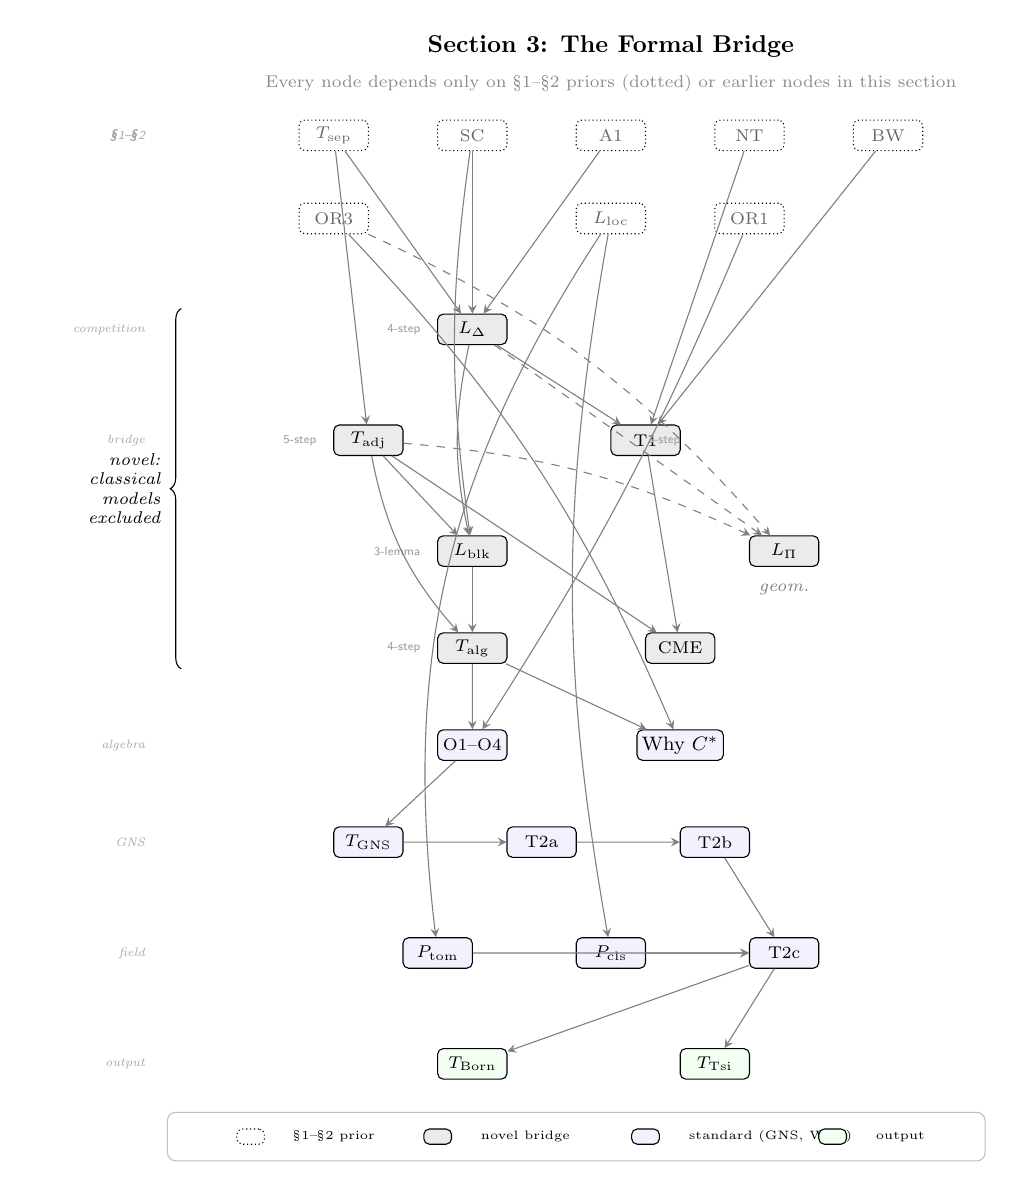
\begin{tikzpicture}[
    scale=0.88, every node/.style={transform shape},
    nd/.style={draw, rounded corners=2pt, minimum height=0.44cm, minimum width=1.0cm, inner sep=2pt, font=\scriptsize},
    prior/.style={nd, densely dotted, text=black!60},
    bridge/.style={nd, fill=black!8},
    skel/.style={nd, fill=blue!5},
    outnode/.style={nd, fill=green!5},
    arr/.style={->, >=stealth, thin, black!50},
    elabel/.style={font=\tiny\itshape, text=black!55, fill=white, inner sep=1pt},
    badge/.style={font=\tiny, text=black!40, anchor=east},
    tier/.style={font=\tiny\itshape, anchor=east, text=black!35},
]

% ── Title ──
\node[font=\normalsize\bfseries, anchor=south] at (1.0, 1.0)
    {Section 3: The Formal Bridge};
\node[font=\scriptsize, anchor=south, text=black!45] at (1.0, 0.5)
    {Every node depends only on \S1--\S2 priors (dotted) or earlier nodes in this section};

% ══════════════════════════════════════════════════════════════════════
% TIER 0: Prior results from §1 and §2 (dotted)
% ══════════════════════════════════════════════════════════════════════
\node[tier] at (-5.6, 0) {{\fontsize{5}{6}\selectfont\textsf{\S1--\S2}}};
\node[prior] (Tsep) at (-3.0, 0) {$T_{\mathrm{sep}}$};
\node[prior] (SC) at (-1.0, 0) {SC};
\node[prior] (A1) at (1.0, 0) {A1};
\node[prior] (NT) at (3.0, 0) {NT};
\node[prior] (BW) at (5.0, 0) {BW};

% Second row of priors
\node[prior] (OR3) at (-3.0, -1.2) {OR3};
\node[prior] (Lloc) at (1.0, -1.2) {$L_{\mathrm{loc}}$};
\node[prior] (OR1) at (3.0, -1.2) {OR1};

% ══════════════════════════════════════════════════════════════════════
% TIER 1: Superadditivity
% ══════════════════════════════════════════════════════════════════════
\node[tier] at (-5.6, -2.8) {{\fontsize{5}{6}\selectfont competition}};
\node[bridge] (LDelta) at (-1.0, -2.8) {$L_\Delta$};
\node[badge] at ($(LDelta.west)+(-0.12,0)$) {\textsf{4-step}};

% ══════════════════════════════════════════════════════════════════════
% TIER 2: Order-dependence + self-adjointness
% ══════════════════════════════════════════════════════════════════════
\node[tier] at (-5.6, -4.4) {{\fontsize{5}{6}\selectfont bridge}};
\node[bridge] (T1) at (1.5, -4.4) {T1};
\node[bridge] (Tadj) at (-2.5, -4.4) {$T_{\mathrm{adj}}$};
\node[badge] at ($(T1.east)+(0.12,0)$) {\textsf{3-step}};
\node[badge] at ($(Tadj.west)+(-0.12,0)$) {\textsf{5-step}};

% ══════════════════════════════════════════════════════════════════════
% TIER 3: Noncommutativity
% ══════════════════════════════════════════════════════════════════════
\node[bridge] (Lblk) at (-1.0, -6.0) {$L_{\mathrm{blk}}$};
\node[bridge] (LPi) at (3.5, -6.0) {$L_\Pi$};
\node[badge] at ($(Lblk.west)+(-0.12,0)$) {\textsf{3-lemma}};
\node[font=\scriptsize\itshape, gray, anchor=north] at (3.5, -6.35) {geom.};

\node[bridge] (Talg) at (-1.0, -7.4) {$T_{\mathrm{alg}}$};
\node[bridge] (CME) at (2.0, -7.4) {CME};
\node[badge] at ($(Talg.west)+(-0.12,0)$) {\textsf{4-step}};

% ══════════════════════════════════════════════════════════════════════
% TIER 4: Algebra assembly
% ══════════════════════════════════════════════════════════════════════
\node[tier] at (-5.6, -8.8) {{\fontsize{5}{6}\selectfont algebra}};
\node[skel] (O1O4) at (-1.0, -8.8) {O1--O4};
\node[skel] (WhyC) at (2.0, -8.8) {\footnotesize Why $C^*$};

% ══════════════════════════════════════════════════════════════════════
% TIER 5: GNS + Wedderburn
% ══════════════════════════════════════════════════════════════════════
\node[tier] at (-5.6, -10.2) {{\fontsize{5}{6}\selectfont GNS}};
\node[skel] (GNS) at (-2.5, -10.2) {$T_{\mathrm{GNS}}$};
\node[skel] (T2a) at (0.0, -10.2) {T2a};
\node[skel] (T2b) at (2.5, -10.2) {T2b};

% ══════════════════════════════════════════════════════════════════════
% TIER 6: Field selection
% ══════════════════════════════════════════════════════════════════════
\node[tier] at (-5.6, -11.8) {{\fontsize{5}{6}\selectfont field}};
\node[skel] (Ptom) at (-1.5, -11.8) {$P_{\mathrm{tom}}$};
\node[skel] (Pcls) at (1.0, -11.8) {$P_{\mathrm{cls}}$};
\node[skel] (T2c) at (3.5, -11.8) {T2c};

% ══════════════════════════════════════════════════════════════════════
% TIER 7: Outputs
% ══════════════════════════════════════════════════════════════════════
\node[tier] at (-5.6, -13.4) {{\fontsize{5}{6}\selectfont output}};
\node[outnode] (TBorn) at (-1.0, -13.4) {$T_{\mathrm{Born}}$};
\node[outnode] (Ttsi) at (2.5, -13.4) {$T_{\mathrm{Tsi}}$};

% ══════════════════════════════════════════════════════════════════════
% ARROWS
% ══════════════════════════════════════════════════════════════════════

% --- §2 priors → L_Δ ---
\draw[arr] (Tsep) -- (LDelta);
\draw[arr] (SC) -- (LDelta);
\draw[arr] (A1) -- (LDelta);

% --- §2 priors → T1 ---
\draw[arr] (LDelta) -- (T1);
\draw[arr] (NT) -- (T1);
\draw[arr] (BW) -- (T1);

% --- §2 priors → T_adj ---
\draw[arr] (Tsep) -- (Tadj);

% --- → L_blk ---
\draw[arr] (Tadj) -- (Lblk);
\draw[arr] (LDelta) to[bend right=12] (Lblk);
\draw[arr] (SC) to[bend right=8] (Lblk);

% --- → L_Π (non-critical, dashed) ---
\draw[arr, gray, dashed] (LDelta) -- (LPi);
\draw[arr, gray, dashed] (Tadj) to[bend left=10] (LPi);
\draw[arr, gray, dashed] (OR3) to[bend left=12] (LPi);

% --- → T_alg ---
\draw[arr] (Lblk) -- (Talg);
\draw[arr] (Tadj) to[bend right=15] (Talg);

% --- → CME ---
\draw[arr] (Tadj) -- (CME);
\draw[arr] (T1) -- (CME);

% --- → O1-O4 ---
\draw[arr] (Talg) -- (O1O4);
\draw[arr] (OR1) to[bend left=5] (O1O4);

% --- → Why C* ---
\draw[arr] (OR3) to[bend left=10] (WhyC);
\draw[arr] (Talg) -- (WhyC);

% --- → GNS / T2a / T2b ---
\draw[arr] (O1O4) -- (GNS);
\draw[arr] (GNS) -- (T2a);
\draw[arr] (T2a) -- (T2b);

% --- → P_tom, P_cls (from L_loc in §2) ---
\draw[arr] (Lloc) to[bend right=20] (Ptom);
\draw[arr] (Lloc) to[bend right=10] (Pcls);

% --- → T2c ---
\draw[arr] (T2b) -- (T2c);
\draw[arr] (Ptom) -- (T2c);
\draw[arr] (Pcls) -- (T2c);

% --- → outputs ---
\draw[arr] (T2c) -- (TBorn);
\draw[arr] (T2c) -- (Ttsi);

% ══════════════════════════════════════════════════════════════════════
% SCOPE BRACE: novel content
% ══════════════════════════════════════════════════════════════════════
\draw[decorate, decoration={brace, amplitude=4pt, mirror}]
    (-5.2, -2.5) -- (-5.2, -7.7)
    node[midway, left=5pt, font=\scriptsize\itshape, text width=1.8cm, align=right]
    {novel:\\classical\\models\\excluded};

% ══════════════════════════════════════════════════════════════════════
% LEGEND
% ══════════════════════════════════════════════════════════════════════
\draw[black!25, rounded corners=3pt] (-5.4, -14.8) rectangle (6.4, -14.1);
\node[prior, minimum width=0.4cm, minimum height=0.22cm] at (-4.2, -14.45) {};
\node[font=\tiny, anchor=west] at (-3.7, -14.45) {\S1--\S2 prior};
\node[bridge, minimum width=0.4cm, minimum height=0.22cm] at (-1.5, -14.45) {};
\node[font=\tiny, anchor=west] at (-1.0, -14.45) {novel bridge};
\node[skel, minimum width=0.4cm, minimum height=0.22cm] at (1.5, -14.45) {};
\node[font=\tiny, anchor=west] at (2.0, -14.45) {standard (GNS, W--A)};
\node[outnode, minimum width=0.4cm, minimum height=0.22cm] at (4.2, -14.45) {};
\node[font=\tiny, anchor=west] at (4.7, -14.45) {output};

\end{tikzpicture}
\caption[Formal bridge DAG]{%
\textbf{Formal bridge: complete dependency structure of Section~3.}
Dotted nodes are results from \S1--\S2 (axiom, definitions, structural lemmas);
all other nodes are proved in this section.
The derivation is strictly acyclic: every node depends only on nodes above it.
\emph{No result from \S4 or later is used.}
The novel bridge chain (left brace) is where all classical models are excluded;
the algebra assembly and GNS steps are standard finite-dimensional mathematics
applied to the derived enforcement structures.
$L_\Pi$ (dashed) provides geometric strengthening but is not on the critical path.
}
\label{fig:formal_bridge_dag}
\end{figure}


\smallskip\noindent\textit{Algebraic infrastructure: where each structural requirement is verified.}  The bridge constructs a finite-dimensional $C^*$-algebra from cost data.  Each structural requirement is verified with a complete proof at a specific location within this section: associative product on enforcement operators (Proposition~O3: closure under composition inherited from $\mathrm{End}(V)$); $*$-involution and self-adjointness (Theorem~$T_{\mathrm{adj}}$, five-step proof; Step~3 corresponds to Lemma~$L_\omega$ in the Formal Supplement); positivity of the state functional (Proposition~O4: two constructions --- normalized trace $\tau$ and cost functional $\omega$ --- both verified positive and faithful); $C^*$-identity and operator norm (``Why $C^*$ specifically'': $\|A\|^2 = \|A^*A\|$ from operator norm on $\mathrm{End}(V)$, completeness automatic in finite dimension); non-circularity of the derivation order (Linear Structure Provenance table, Box~\ref{box:provenance}); and an independent categorical route via sequential effect algebras with Gudder--Greechie and van de Wetering hypothesis verification (Appendix~\ref{app:sea}).

\subsection{\texorpdfstring{$L_{\Delta}$}{L Delta} (Competition): superadditivity from substrate integrity}
\label{thm:ldelta}\label{sec:L_Delta}

\smallskip\noindent\textit{Non-closure hierarchy: two levels, one condition separating them.}  The passage to quantum structure rests on a two-level ladder, and it is worth naming the levels before proving the second.

\textbf{Level~1 --- Weak non-closure} ($L_{\mathrm{nc}}$, proved in Section~\ref{sec:defs}): A1 alone forces
\[
E(A \cup B) \;\ge\; E(A) + E(B)
\]
for some pairs $A, B$ (the Minkowski overflow argument).  The inequality may be tight: additive costs are possible when no shared substrate couples $A$ and $B$.  No perturbation structure, no geometry, no $T_{\mathrm{sep}}$.  This is the universal, classical level.

\textbf{Level~2 --- Strict superadditivity} ($L_\Delta$, proved below): A1 + separated anchor geometry ($T_{\mathrm{sep}}$) forces
\[
\varepsilon(\{d_1,d_2\}) \;\ge\; \varepsilon(d_1) + \varepsilon(d_2) + \Delta_\Gamma, \qquad \Delta_\Gamma > 0,
\]
for co-located distinctions with disjoint mechanisms.  The single condition separating Level~1 from Level~2 is $T_{\mathrm{sep}}$ --- the disjoint-anchor condition.  When $M_{d_1} \cap M_{d_2} \ne \{0\}$, $\Delta$ can vanish (mechanisms overlap, shared resources can be reused); when $M_{d_1} \cap M_{d_2} = \{0\}$, $\Delta > 0$ is forced by the presence of shared substrate beyond the two mechanisms.  The gap between the two levels is geometry.

Pause here and take stock.  $L_{\mathrm{nc}}$ says that two individually affordable collections of distinctions can be jointly unaffordable---a finite budget overflows when you try to maintain everything at once.  This is a real constraint, but it is entirely classical: a shipping container has finite volume, and two loads that each fit individually may not fit together.  Nothing about non-closure, by itself, produces interference, noncommutativity, or any distinctively quantum phenomenon.  Classical budget overflow gives you a knapsack problem.  It does not give you quantum mechanics.

The passage from ``finite budget'' to ``noncommutativity'' requires something stronger: that jointly enforcing two distinctions costs \emph{strictly more} than the sum of individual costs---that is, superadditivity.  The additional cost has a simple origin: at a shared interface, you pay for the house, not just the rooms.

\smallskip\noindent\textit{Why finite capacity alone does not force strict superadditivity --- and what does.}  A1 by itself does not force strict superadditivity: $L_{\mathrm{nc}}$ shows that additive costs ($\Delta = 0$) are consistent with A1 alone.  Many bounded-resource systems exhibit purely additive costs up to saturation: two independent processes sharing a CPU time budget, two gas containers sharing a pressure reservoir, two radio transmitters sharing a frequency band.  In each case, the joint cost is the sum of individual costs, with no premium, until the total exceeds the bound.  The reason is that these systems lack co-located shared infrastructure: the processes do not couple through a common physical substrate that itself requires maintenance.  What forces $\Delta > 0$ is a geometric fact about non-degenerate interfaces: the shared substrate pool $\Pi$ carries a distinction of its own---pool integrity---that must be jointly maintained whenever two mechanism-disjoint distinctions share an interface.  That pool-integrity distinction has positive enforcement cost by A1, and its anchor set is disjoint from both mechanism sectors by construction.  Cost additivity over disjoint anchor sets then forces the total to exceed the sum.  The key structural input beyond A1 is therefore $T_{\mathrm{sep}}$ + CL1--CL3: these identify the specific geometric configuration (disjoint mechanisms at a shared interface with residual substrate) under which the pool-integrity distinction is forced to exist and to be costly.

% ======================================================================
% Co-location definition (kept from v15)
% ======================================================================

\begin{tcolorbox}[apfbox, title={$L_{\Delta}$ (Competition): Superadditivity from Substrate Integrity}]
\textit{Co-located distinctions with disjoint mechanisms cost strictly more together than apart: the shared substrate exacts a positive premium.}

\smallskip\noindent\textbf{Definition (Co-located distinctions).}  Distinctions $d_1, d_2 \in \mathcal{D}$ are \emph{co-located at $\Gamma$} if and only if:
\begin{enumerate}[nosep,leftmargin=2em,itemsep=2pt,label=(\textbf{CL\arabic*})]
  \item $M_{d_1}, M_{d_2} \subseteq S_\Gamma$: both anchor sets are subsets of the same interface substrate.
  \item $M_{d_1} \cap M_{d_2} = \{0\}$: the anchor sets are disjoint within $S_\Gamma$ (i.e., $T_{\mathrm{sep}}$ holds for this pair).
  \item $\Pi := S_\Gamma \setminus (M_{d_1} \oplus M_{d_2}) \ne \emptyset$: the substrate has degrees of freedom beyond the two anchor sets.
\end{enumerate}
CL1 says both distinctions draw from the same budget; CL2 says they do so through distinct mechanisms; CL3 says the interface is not exhausted by these two anchor sets alone.

\smallskip\noindent\textbf{Lemma (CL3 from interface structure).}\label{prop:generic_coloc}
\textit{Let $d_1, d_2 \in \mathcal{D}(\Gamma)$ satisfy CL1 and CL2.  If $n_{\max}(\Gamma) := \lfloor C(\Gamma)/\varepsilon^*\rfloor \ge 3$, then $\Pi \ne \emptyset$.}

\smallskip\noindent\textit{Proof.}  By CL2, $M_{d_1} \cap M_{d_2} = \{0\}$, so $M_{d_1} \oplus M_{d_2}$ consumes $\dim(M_{d_1}) + \dim(M_{d_2}) \ge 2$ independent substrate dimensions, costing at least $2\varepsilon^*$ by $L_{\mathrm{cost}}$ (MD).  Since $n_{\max} \ge 3$, the interface capacity satisfies $C(\Gamma) \ge 3\varepsilon^*$, so at least $\varepsilon^*$ of budget---and at least one substrate dimension---remains beyond $M_{d_1} \oplus M_{d_2}$.  That residual substrate is~$\Pi$.  \hfill$\square$

% ======================================================================
% PRIMARY PROOF: substrate-integrity argument
% ======================================================================

\medskip\noindent\textbf{Statement.}  Let $d_1, d_2 \in \mathcal{D}(\Gamma)$ be co-located (CL1--CL3).  Then:
\begin{equation}\label{eq:Ldelta}
\varepsilon(\{d_1, d_2\}) \;=\; \varepsilon(d_1) + \varepsilon(d_2) + \Delta(d_1, d_2), \qquad \Delta(d_1, d_2) \;=\; \varepsilon(d_\Gamma) \;>\; 0.
\end{equation}
Additivity ($\Delta = 0$) and subadditivity ($\Delta < 0$) are both excluded.

\smallskip\noindent\textbf{\textit{Variables:}}
\begin{varlist}
\item $\varepsilon(\{d_1, d_2\})$ --- the joint enforcement cost: minimum cost of maintaining \emph{both} $d_1$ and $d_2$ simultaneously at~$\Gamma$.
\item $d_\Gamma$ --- the \emph{substrate-integrity distinction}: the binary predicate on $\Pi$ that is true when the pool state is compatible with joint enforcement of $d_1$ and $d_2$, and false when the pool mediates corruption between the two mechanism sectors.
\item $\varepsilon(d_\Gamma) > 0$ --- the enforcement cost of substrate integrity (positive by A1).
\item $\Delta(d_1, d_2) := \varepsilon(\{d_1,d_2\}) - \varepsilon(d_1) - \varepsilon(d_2)$ --- the superadditivity surplus.
\end{varlist}

\smallskip\noindent\textbf{Depends on.}  A1 (finite budget), SC (every direction anchors a distinction; \S\ref{sec:defs}), $T_{\mathrm{sep}}$ (disjoint anchors $\Leftrightarrow$ additive costs; \S\ref{sec:defs}), CL1--CL3 (co-location geometry; derived for $n_{\max} \ge 3$).

\smallskip\noindent\textbf{Status.}  \textbf{[Proved]} --- substrate-integrity argument (4 steps) below, plus independent LP verification.

\smallskip\noindent\textbf{Proof} (substrate integrity).

\textit{Step 1 (Substrate-integrity distinction exists).}  By CL3, $\Pi \ne \emptyset$: the interface substrate contains degrees of freedom outside $M_{d_1} \oplus M_{d_2}$.  The pool $\Pi$ is physically coupled to both mechanism sectors (they share a common interface substrate $S_\Gamma$ by CL1).  The binary predicate $d_\Gamma: S_\Gamma \to \{0,1\}$ defined by
\[
d_\Gamma(\sigma) \;=\; 
\begin{cases}
1 & \text{if } \sigma|_\Pi \text{ is compatible with joint enforcement of } d_1, d_2, \\
0 & \text{otherwise}
\end{cases}
\]
is a non-trivial distinction supported on $\Pi$.  Concretely: $d_\Gamma$ is true when the pool state does not mediate uncontrolled coupling between $M_{d_1}$ and $M_{d_2}$, and false when it does.  By SC (Substrate Completeness), every non-trivial predicate on a non-empty subspace of $S_\Gamma$ is a distinction in $\mathcal{D}$.  Therefore $d_\Gamma \in \mathcal{D}(\Gamma)$.

\textit{Step 2 (Positive cost).}  By A1 (physicality criterion): $\varepsilon(d_\Gamma) > 0$.  The pool degrees of freedom in $\Pi$ are physically present and coupled to both mechanism sectors.  Maintaining pool integrity against this coupling is a non-trivial enforcement act; it is not free.

\textit{Step 3 (Anchor disjointness).}  The anchor set $M_{d_\Gamma} \subseteq \Pi$ by construction: $d_\Gamma$ is a predicate on the pool state, so its enforcement mechanism lies entirely within~$\Pi$.  Since $\Pi \cap M_{d_1} = \emptyset$ and $\Pi \cap M_{d_2} = \emptyset$ (by the definition of $\Pi$ as the complement of $M_{d_1} \oplus M_{d_2}$ within $S_\Gamma$):
\[
M_{d_\Gamma} \cap M_{d_1} = \{0\}, \qquad M_{d_\Gamma} \cap M_{d_2} = \{0\}.
\]
The triple $(d_1, d_2, d_\Gamma)$ is pairwise independently enforceable: all three anchor sets are mutually disjoint.

\textit{Step 4 (Joint enforcement entails substrate integrity).}  Jointly enforcing $d_1$ and $d_2$ at a shared interface requires that the pool state not corrupt either mechanism sector.  If $d_\Gamma$ fails---if the pool mediates uncontrolled coupling between $M_{d_1}$ and $M_{d_2}$---then the joint configuration $\{d_1, d_2\}$ cannot be maintained, regardless of the resources committed to each mechanism individually.  (A freely evolving subsystem coupled to two mechanism sectors generically mediates interactions between them; preventing this is the physical content of substrate integrity.)  Therefore:
\[
\text{Joint enforcement of } \{d_1, d_2\} \quad\Longrightarrow\quad \text{enforcement of } d_\Gamma.
\]

\textit{Step 5 (Cost additivity over disjoint mechanisms).}  By Step~3, the three anchor sets $M_{d_1}$, $M_{d_2}$, and $M_{d_\Gamma}$ are pairwise disjoint.  By $T_{\mathrm{sep}}$ and cost additivity (disjoint anchors have additive costs, the exact-accounting condition for independently enforceable families):
\[
\varepsilon(\{d_1, d_2, d_\Gamma\}) \;=\; \varepsilon(d_1) + \varepsilon(d_2) + \varepsilon(d_\Gamma).
\]

\textit{Step 6 (Superadditivity).}  By Step~4, joint enforcement of $\{d_1, d_2\}$ entails enforcement of $d_\Gamma$.  Therefore the joint enforcement cost satisfies:
\[
\varepsilon(\{d_1, d_2\}) \;\ge\; \varepsilon(d_1) + \varepsilon(d_2) + \varepsilon(d_\Gamma).
\]
The reverse inequality $\varepsilon(\{d_1,d_2\}) \le \varepsilon(d_1) + \varepsilon(d_2) + \varepsilon(d_\Gamma)$ holds because the strategy ``defend each mechanism sector and defend the pool'' is a feasible joint defense.  Therefore equality holds, and:
\begin{equation}
\Delta(d_1, d_2) \;=\; \varepsilon(d_\Gamma) \;\ge\; \varepsilon^* \;>\; 0. \qquad\square
\end{equation}

\medskip\noindent\textbf{Exclusion of additivity and subadditivity.}

\textit{Additivity excluded} ($\Delta = 0$ impossible under CL1--CL3).  Additivity requires $\varepsilon(d_\Gamma) = 0$.  By A1, $\varepsilon(d_\Gamma) > 0$ for any non-trivial distinction.  The substrate-integrity distinction is non-trivial whenever $\Pi \ne \emptyset$ (CL3) and the pool is coupled to both mechanism sectors (CL1).  \hfill$\square_{\mathrm{add}}$

\textit{Subadditivity excluded} ($\Delta < 0$ impossible).  Subadditivity would require $\varepsilon(\{d_1,d_2\}) < \varepsilon(d_1) + \varepsilon(d_2)$.  But $T_{\mathrm{sep}}$ gives exact cost additivity for disjoint mechanisms: the cost of maintaining $d_1$ and $d_2$ is \emph{at least} $\varepsilon(d_1) + \varepsilon(d_2)$, since mechanism-localized threats to each must still be individually countered.  (Defense budget in $M_{d_1}$ has no value against threats in $M_{d_2}$ when $M_{d_1} \cap M_{d_2} = \{0\}$.)  Therefore $\varepsilon(\{d_1,d_2\}) \ge \varepsilon(d_1) + \varepsilon(d_2)$, and subadditivity is impossible.  \hfill$\square_{\mathrm{sub}}$

\medskip\noindent\textbf{Counterfactual table.}  Strict superadditivity fails when the non-degenerate interface condition is violated:

\smallskip
\begin{tabular}{@{}p{3.8cm}p{8.8cm}@{}}
\hline\noalign{\smallskip}
\textbf{Condition violated} & \textbf{Why $\Delta = 0$ becomes possible} \\[2pt]
$n_{\max} \le 2$ (degenerate) & CL3 fails: $\Pi = \emptyset$; no substrate-integrity distinction; $\Delta = 0$ \\
Mechanisms overlap ($\notin \mathcal{D}_{\mathrm{ind}}$) & CL2 fails: shared mechanism resources can absorb pool coupling; $d_\Gamma$ becomes redundant \\
$L_{\mathrm{loc}}$ violated & Budget can be borrowed from a neighboring interface to cover $\varepsilon(d_\Gamma)$ at zero marginal cost to $\Gamma$ \\
\end{tabular}

\medskip\noindent\textit{Scope.}  A1 alone forces weak non-closure ($\Delta \ge 0$, $L_{\mathrm{nc}}$).  Strict positivity ($\Delta > 0$) is a theorem at every non-degenerate interface ($n_{\max} \ge 3$).  The classical limit ($\Delta = 0$) is the degenerate boundary $n_{\max} \le 2$, not a separate physical regime.

\coderef{check\_L\_Delta}{paper1.py}\,%
\hspace{1em}\textit{(also verified in \texttt{supplement.py})}
\end{tcolorbox}
% ======================================================================


\medskip\noindent\textbf{Corollary (Regime Biconditional): Exact Trigger for $L_\Delta$.}

\textbf{Statement.}  Let $d_1, d_2 \in \mathcal{D}(\sigma,\Gamma)$.  Strict superadditivity $\Delta(d_1,d_2) > 0$ holds \emph{if and only if} the co-location conditions are satisfied:
\[
\Delta(d_1,d_2) > 0 \;\iff\; \underbrace{M_{d_1},\, M_{d_2} \subseteq S_\Gamma}_{\text{CL1: shared budget}} \;\wedge\; \underbrace{M_{d_1} \cap M_{d_2} = \{0\}}_{\text{CL2: distinct mechanisms}} \;\wedge\; \underbrace{\Pi \ne \emptyset}_{\text{CL3: non-empty pool}}.
\]
The three failure modes are: (i) different interfaces ($\neg$CL1): independent budgets, $\Delta = 0$ ($L_{\mathrm{loc}}$); (ii) mechanism overlap ($\neg$CL2): classical regime; (iii) $\Pi = \emptyset$ ($\neg$CL3): no pool, no integrity distinction, $\Delta = 0$.

\smallskip\noindent\textbf{Counterexample class: architectural redundancy and synergy.}

A natural objection is that many physical systems exhibit \emph{sub}additive joint costs: two processes sharing a cache, two logical qubits sharing a physical ancilla, two sensors sharing a reference clock.  In each case, the joint cost is \emph{less} than the sum of individual costs because shared infrastructure is reused rather than duplicated.  Does this contradict $L_\Delta$?

No.  These are all instances of \emph{mechanism overlap} ($\neg$CL2): the shared resource (cache, ancilla, clock) lies in $M_{d_1} \cap M_{d_2} \ne \{0\}$, so CL2 fails and $L_\Delta$ does not apply.  The APF handles this regime explicitly: when mechanisms overlap, the enforcement cost is \emph{subadditive} ($\Delta \le 0$), the shared resource absorbs what would otherwise be a pool-integrity cost, and the resulting algebra is commutative within the overlapping sector.  Three concrete instances:

\smallskip\noindent\textit{(i) Shared ancilla (QEC).}  Two logical qubits sharing a physical ancilla for syndrome extraction have $M_{d_1} \cap M_{d_2} \supseteq \{\text{ancilla}\} \ne \{0\}$.  The joint extraction cost is less than twice the individual cost because the ancilla is prepared once, not twice: $\varepsilon(\{d_1,d_2\}) < \varepsilon(d_1) + \varepsilon(d_2)$, so $\Delta < 0$.  CL2 fails; $L_\Delta$ does not apply.

\smallskip\noindent\textit{(ii) Classical multiplexing.}  Two radio signals sharing a frequency band (time-division multiplexing) have overlapping physical substrates: the same electromagnetic mode carries both.  The joint transmission cost is subadditive because the carrier infrastructure (oscillator, amplifier) is shared.  CL2 fails; the resulting observable algebra is commutative ($\ell^\infty(X)$), exactly as APF predicts for the $\neg$CL2 regime.


\subsubsection*{Constructive verifications}

The primary proof above establishes $\Delta > 0$ from the existence and positive cost of $d_\Gamma$.  Three independent constructive verifications --- an LP decomposition pinning $\Delta = \varepsilon(d_\Gamma)$ exactly, two microphysical witnesses (Ising interface and shared-ancilla model), and an explicit toy model computing $\Delta$ from the perturbation cost function $\kappa$ --- are in Section~\ref{sec:Ldelta_verifications}.  They provide quantitative checks but are not on the critical path.

The substrate-integrity distinction $d_\Gamma$ (``the pool state $e_3$ is compatible with joint enforcement'') has anchor set $M_{d_\Gamma} = \mathrm{span}\{e_3\} = \Pi$, disjoint from both $M_{d_1}$ and $M_{d_2}$.  Its perturbation class $\mathcal{P}(d_\Gamma) = \{p : p|_\Pi \ne \mathrm{Id}|_\Pi,\; p|_{\Pi^\perp} = \mathrm{Id}\}$; every such $p$ has $\mathrm{rank}(p - \mathrm{Id}) = 1$, so $\varepsilon(d_\Gamma) = \varepsilon^*$.

\smallskip\noindent\textbf{Joint enforcement cost.}  The joint perturbation class $\mathcal{P}(\{d_1, d_2\})$ includes all maps $p$ that can destroy either $d_1$ or $d_2$ or the integrity of their joint configuration.  Defending against $\mathcal{P}(\{d_1, d_2\})$ requires defending $M_{d_1}$, $M_{d_2}$, \emph{and} $\Pi$ simultaneously.  The three anchor sets are pairwise disjoint ($T_{\mathrm{sep}}$), so by K3 the minimum joint defense cost is:
\[
D(\mathcal{P}(\{d_1,d_2\})) \;=\; \varepsilon(d_1) + \varepsilon(d_2) + \varepsilon(d_\Gamma) \;=\; 3\varepsilon^*.
\]
Therefore:
\[
\Delta \;=\; \varepsilon(\{d_1,d_2\}) - \varepsilon(d_1) - \varepsilon(d_2) \;=\; 3\varepsilon^* - 2\varepsilon^* \;=\; \varepsilon^* \;>\; 0.
\]

\smallskip\noindent\textbf{Why $\Delta = 0$ is impossible in this model.}  Suppose the joint defense could be achieved by defending only $M_{d_1}$ and $M_{d_2}$ (cost $2\varepsilon^*$), ignoring $\Pi$.  Then the pool dimension $e_3$ is undefended: a perturbation $p \in \mathcal{P}(d_\Gamma)$ acting on $e_3$ alone could corrupt the joint configuration at zero marginal cost.  Such a perturbation exists (any rank-1 map altering $e_3$) and has $\kappa(p) = \varepsilon^* > 0$, which must be budgeted.  Therefore the defense at $2\varepsilon^*$ is incomplete, and the true minimum is $3\varepsilon^*$.


\subsubsection*{From order-sensitive enforcement updates to a noncommutative operator algebra}

\smallskip\noindent\textit{Why T1 alone does not give noncommutativity.}  The classical Bayesian countermodel (path-dependent conditioning on a commutative $\sigma$-algebra) shows that T1's order-dependence criterion is satisfiable by a commutative model.  The passage from operational order-dependence to algebraic noncommutativity requires OR2 (the $*$-involution with self-adjoint generators, proved as $T_{\mathrm{adj}}$); once OR2 is in place, the GNS computation forces $\mathcal{A}$ to be noncommutative.  T1 contributes distinct operators $E_{d_1} \ne E_{d_2}$ (O2); OR2 is what rules out all commutative models.

\begin{tcolorbox}[apfbox, title={Theorem T1 --- The Bridge Theorem (Order-Dependence)}]
\textit{Superadditivity makes the order in which you enforce distinctions physically observable: different orderings leave different residual states.}

\smallskip\noindent\textbf{Statement.}  $L_\Delta$ + NT + OR0 + BW $\implies$ there exist distinctions $d_1, d_2, d_3 \in \mathcal{D}$ and an initial state $\sigma_0 \in \Omega$ such that
\[
(\mathfrak{E}_{d_3} \circ \mathfrak{E}_{d_1})(\sigma_0) \;\ne\; (\mathfrak{E}_{d_3} \circ \mathfrak{E}_{d_2})(\sigma_0) \quad \in\; \Omega \cup \{\bot\},
\]
where $\bot$ is the enforcement-failure state (budget exceeded).  In particular, $\mathfrak{E}_{d_1}$ and $\mathfrak{E}_{d_2}$ are not interchangeable as operations on $\Omega$: composing from the left with $\mathfrak{E}_{d_3}$ distinguishes them.

\smallskip\noindent\textbf{Premises.}
\begin{varlist}
\item $L_\Delta$: distinctions $d_1, d_2$ co-located at $\Gamma$ satisfy $\Delta(d_1,d_2) > 0$.
\item NT (proved from $L_{\mathrm{cost}}$ + A1's $|\mathcal{D}| \ge 2$): there exist $d_1, d_2 \in \mathcal{D}$ with $\varepsilon(d_1) \ne \varepsilon(d_2)$.
\item OR0 (Faithfulness): distinct residual enforceability structures correspond to distinct states in $\Omega$ (definitional; see Section~\ref{sec:defs}).
\item \textbf{BW (Budget-Window, joint-admissibility form):}  There exists a triple $(d_1, d_2, d_3) \in \mathcal{D}^3$ with $\varepsilon(d_1) < \varepsilon(d_2)$ such that $\{d_1, d_3\}$ is jointly admissible but $\{d_2, d_3\}$ is not:
\[
\varepsilon(\{d_1, d_3\}) \;\le\; C \quad\text{and}\quad \varepsilon(\{d_2, d_3\}) \;>\; C.
\]
Here $\varepsilon(\{d_i, d_3\})$ is the \emph{joint} enforcement cost under A1, including any superadditivity surplus: $\varepsilon(\{d_i,d_3\}) = \varepsilon(d_i) + \varepsilon(d_3) + \Delta(d_i,d_3)$.  The condition is purely about which joint states are admissible.

\textit{Relation to the plain-cost window.}  The special case $\Delta(d_1,d_3) = \Delta(d_2,d_3) = 0$ recovers the plain-cost form $C - \varepsilon(d_1) \ge \varepsilon(d_3) > C - \varepsilon(d_2)$.  The joint-admissibility form is general.

\textit{Status.}  BW is a richness condition on the joint-cost spectrum --- the only premise of T1 not derived from A1 within this paper.  It requires that the cost spectrum be dense enough to contain a distinction $d_3$ in the budget window $(C - \varepsilon(\{d_2,d_3\}),\; C - \varepsilon(\{d_1,d_3\})]$.  BW is \emph{not} derivable from A1 + $n_{\max} \ge 3$ alone: the cost-spectrum density is a property of the physical field content, not of the budget bound.  It is subsequently confirmed by Paper~2's derivation of 61 independent capacity types (with costs spanning the full range of integer multiples of $\varepsilon^*$), which provides far more triples than needed.  Within Paper~1, T1 is conditional on BW; the worked example (Section~\ref{sec:worked_example}) exhibits a concrete satisfying instance with $C = 5$, $\varepsilon(d_1) = 2$, $\varepsilon(d_2) = 3$, $\varepsilon(d_3) = 5/2$.
\end{varlist}

\smallskip\noindent\textbf{\textit{Variables:}}
\begin{varlist}
\item $\mathfrak{E}_{d}: \Omega \to \Omega \cup \{\bot\}$ --- the enforcement partial map for $d$: maps $\sigma$ to $\sigma'$ in which $d$ is active, budget reduced by $\varepsilon(d)$ plus superadditivity surplus with already-active distinctions, and residual enforceability updated.  Maps to $\bot$ if budget is insufficient.
\item $m(d_2 \mid d_1)$ --- the marginal cost of $d_2$ given $d_1$ is already enforced: $m(d_2 \mid d_1) = \varepsilon(\{d_1, d_2\}) - \varepsilon(d_1)$.
\item $\Delta(d_1, d_2) = \varepsilon(\{d_1, d_2\}) - \varepsilon(d_1) - \varepsilon(d_2) > 0$ --- the superadditivity surplus (positive by $L_\Delta$).
\end{varlist}

\smallskip\noindent\textbf{Status.}  \textbf{[Proved]} from $L_\Delta$ + NT + OR0 + BW.  Three-step proof below.  A Bayesian countermodel after the proof shows T1 alone does not force noncommutativity.

\smallskip\noindent\textbf{Proof} (three steps).

\textit{Step 1} (Superadditivity forces context-dependent marginal costs).  By $L_\Delta$, $\Delta(d_1, d_2) > 0$ for distinctions sharing enforcement resources.  Therefore:
\begin{equation}
m(d_2 \mid d_1) = \varepsilon(d_2) + \Delta \;>\; \varepsilon(d_2) = m(d_2 \mid \emptyset).
\end{equation}
The marginal cost of enforcing $d_2$ depends on whether $d_1$ is already enforced.  This is \emph{not} a bookkeeping artifact: $\mathfrak{E}_{d_2}$ consumes a different budget (and leaves a different residual state) depending on the prior state.

\textit{Step 2} (NT + BW produce asymmetric residual budgets).  Let $(d_1, d_2, d_3)$ be the BW triple.  WLOG $\varepsilon(d_1) < \varepsilon(d_2)$.  Take initial state $\sigma_0 = \sigma_\emptyset$ (no distinctions active, budget $C$).  The two single-enforcement outcomes are:
\begin{align*}
\mathfrak{E}_{d_1}(\sigma_0) &= \sigma_1 := \bigl(\{d_1\},\; C - \varepsilon(d_1)\bigr), \\
\mathfrak{E}_{d_2}(\sigma_0) &= \sigma_2 := \bigl(\{d_2\},\; C - \varepsilon(d_2)\bigr).
\end{align*}
Since $\varepsilon(d_1) < \varepsilon(d_2)$, the residual budgets satisfy $C - \varepsilon(d_1) > C - \varepsilon(d_2)$.  By OR0, $\sigma_1 \ne \sigma_2$ in $\Omega$ (they have different residual budgets, hence different enforceability structures).

\textit{Step 3} (BW witness: direct proof of operational non-commutativity).  Apply $\mathfrak{E}_{d_3}$ to both outcomes.  The enforcement map $\mathfrak{E}_{d_3}$ from state $\sigma_i$ (with $d_i$ already active) requires marginal cost $m(d_3 \mid d_i) = \varepsilon(\{d_i, d_3\}) - \varepsilon(d_i)$.  By the BW condition:
\begin{itemize}[nosep,leftmargin=2em,itemsep=2pt]
  \item \textbf{From $\sigma_1$:} the marginal cost is $m(d_3 \mid d_1) = \varepsilon(\{d_1,d_3\}) - \varepsilon(d_1)$.  Since $\varepsilon(\{d_1,d_3\}) \le C$ (BW), we have $m(d_3 \mid d_1) \le C - \varepsilon(d_1)$, which is exactly the available residual budget in $\sigma_1$.  Enforcement succeeds.
  \item \textbf{From $\sigma_2$:} the marginal cost is $m(d_3 \mid d_2) = \varepsilon(\{d_2,d_3\}) - \varepsilon(d_2)$.  Since $\varepsilon(\{d_2,d_3\}) > C$ (BW) and $\Delta(d_2,d_3) \ge 0$, we have $m(d_3 \mid d_2) > C - \varepsilon(d_2)$, which exceeds the available residual budget in $\sigma_2$.  Enforcement fails.
\end{itemize}
Therefore:
\begin{align}
(\mathfrak{E}_{d_3} \circ \mathfrak{E}_{d_1})(\sigma_0) &= \mathfrak{E}_{d_3}(\sigma_1) = \bigl(\{d_1, d_3\},\; C - \varepsilon(\{d_1,d_3\})\bigr) \;\in\; \Omega, \label{eq:T1_ord1}\\
(\mathfrak{E}_{d_3} \circ \mathfrak{E}_{d_2})(\sigma_0) &= \mathfrak{E}_{d_3}(\sigma_2) = \bot \quad \bigl(\text{marginal cost } \varepsilon(\{d_2,d_3\}) - \varepsilon(d_2) > C - \varepsilon(d_2)\bigr). \label{eq:T1_ord2}
\end{align}
The first lies in $\Omega$ (a valid admissible state with residual budget $C - \varepsilon(\{d_1,d_3\}) \ge 0$); the second is $\bot$ (enforcement failure).  These are distinct elements of $\Omega \cup \{\bot\}$.  \hfill$\square$

\smallskip\noindent\textit{Clarification on the form of non-commutativity.}  Note that both orderings $\mathfrak{E}_{d_1} \circ \mathfrak{E}_{d_2}$ and $\mathfrak{E}_{d_2} \circ \mathfrak{E}_{d_1}$ applied to $\sigma_0$ \emph{both} terminate at $\sigma_{12} = (\{d_1,d_2\}, C - \varepsilon(d_1) - \varepsilon(d_2) - \Delta)$ — the final state is the same.  T1 does \emph{not} claim $(\mathfrak{E}_{d_1} \circ \mathfrak{E}_{d_2})(\sigma_0) \ne (\mathfrak{E}_{d_2} \circ \mathfrak{E}_{d_1})(\sigma_0)$.  The non-commutativity is of a different kind: the operations $\mathfrak{E}_{d_1}$ and $\mathfrak{E}_{d_2}$ are distinguishable by their left-action (their effect on what follows), not their bilateral composition on a single initial state.  Equations \eqref{eq:T1_ord1}--\eqref{eq:T1_ord2} provide this distinction via a three-operation witness.  This is the appropriate notion of non-commutativity for partial maps on $\Omega$; the stronger algebraic noncommutativity $[E_{d_1},E_{d_2}]\ne 0$ in $\mathcal{A}$ is a post-GNS phenomenon, established in T2 and Corollary~$T_{\mathrm{alg}}$ after the matrix representation is in hand.

\smallskip\noindent\textbf{Countermodel (within APF).}  If $\Delta = 0$: marginal costs are context-independent, residual budgets after $d_1$ and $d_2$ still differ (by NT), but the BW witness fails if no $d_3$ is in the budget window --- enforcement is order-independent in the absence of superadditivity.  If NT fails ($\varepsilon(d_1) = \varepsilon(d_2)$): residual budgets are equal, BW cannot hold, and no budget-window witness exists.  If BW fails (cost spectrum has no distinction in the window $(C-\varepsilon(d_2), C-\varepsilon(d_1)]$): no distinguishing continuation exists and the partial maps are indistinguishable by this method.  All four premises are necessary for this witness.

\smallskip\noindent\textbf{Classical Bayesian countermodel (T1 does not establish noncommutativity).}  The order-dependence proved in T1 is also present in classical commutative probability, and therefore T1 alone does not distinguish quantum from classical models.

\textit{Construction.}  Let $(\Omega_{\mathrm{cl}}, \mathcal{F}, P)$ be any classical probability space with events $A, B, C \in \mathcal{F}$ satisfying $P(A), P(B), P(C) > 0$, $P(A \cap C) > 0$, and $P(B \cap C) = 0$.  Define enforcement maps by Bayesian conditioning: $\mathfrak{E}_X(\rho) := \rho(\,\cdot \mid X)$ if $\rho(X) > 0$, and $\bot$ if $\rho(X) = 0$.  Then:
\begin{align*}
(\mathfrak{E}_C \circ \mathfrak{E}_A)(\rho) &= \rho(\,\cdot \mid A \cap C) \;\in\; \Omega_{\mathrm{cl}}, \\
(\mathfrak{E}_C \circ \mathfrak{E}_B)(\rho) &= \bot \quad (P(B \cap C) = 0),
\end{align*}
which is exactly the T1 witness structure: one composition succeeds (lands in $\Omega_{\mathrm{cl}}$) and the other fails (reaches $\bot$), so $\mathfrak{E}_A$ and $\mathfrak{E}_B$ are operationally distinguishable by their effect under left-composition with $\mathfrak{E}_C$.  Yet the underlying algebra of events $\mathcal{F}$ is commutative: as a Boolean $\sigma$-algebra, $A \cap B = B \cap A$, $A \cup B = B \cup A$, and every Boolean algebra is commutative.  Sequential conditioning is path-dependent at the \emph{operational} level but commutative at the \emph{algebraic} level.

\textit{Why this model is excluded.}  The classical Bayesian model fails to satisfy OR2.  In the classical model, the conditioning map $\mathfrak{E}_A: \rho \mapsto \rho(\cdot|A)$ is not self-adjoint in any natural sense: there is no inner product $\langle \cdot, \cdot \rangle_\omega$ on the space of measures for which $\mathfrak{E}_A^* = \mathfrak{E}_A$.  Equivalently, the algebra of conditioning operations on $\mathcal{F}$ is not a $*$-algebra with self-adjoint generators --- it is a monoid of maps with no involution structure.  OR2 asserts exactly what the classical model cannot provide: $E_d^* = E_d$ under the inner product $\langle A, B \rangle_\omega = \omega(A^*B)$.  In a commutative $*$-algebra, every product of self-adjoint elements is self-adjoint; but the GNS computation shows $\sigma_z \sigma_x = i\sigma_y$ is not self-adjoint, which is impossible in any commutative $*$-algebra.  This contradiction, established in $T_{\mathrm{alg}}$, is the precise step that rules out all classical commutative models.

\smallskip\noindent\textbf{Proposition (Classical Model Exclusion, CME).}\label{prop:CME}
\emph{Let $M$ be any classical probabilistic model with finite state space $X$, observable algebra $\mathcal{A}_{\mathrm{cl}} := \ell^\infty(X) \cong \mathbb{R}^{|X|}$, and update maps $T_d : \Delta(X) \to \Delta(X)$ exhibiting T1-type order-dependence.  Then:
\begin{enumerate}[nosep,leftmargin=2em,itemsep=2pt,label=(\roman*)]
  \item $\mathcal{A}_{\mathrm{cl}}$ is commutative: $fg = gf$ for all $f, g \in \mathcal{A}_{\mathrm{cl}}$.
  \item If OR2 holds in $M$ --- i.e.\ the enforcement operators $E_d$ are elements of $\mathcal{A}_{\mathrm{cl}}$ satisfying $E_d^* = E_d$ within $\mathcal{A}_{\mathrm{cl}}$ --- then $[E_{d_1}, E_{d_2}] = 0$: OR2 is incompatible with T1-type order-dependence in any classical model.
  \item Classical models satisfying T1-type order-dependence necessarily represent their update maps in $\mathrm{End}(\Delta(X))$, not in $\mathcal{A}_{\mathrm{cl}}$; such maps cannot satisfy OR2 in $\mathcal{A}_{\mathrm{cl}}$.
\end{enumerate}
Therefore: any model satisfying both OR2 and T1 is not a classical probabilistic model.  The inference from T1 to a noncommutative operator algebra requires OR2; OR2 is precisely the condition classical models fail.}

\smallskip\noindent\textit{Proof.}
\textit{(i)} $\mathcal{A}_{\mathrm{cl}} = \ell^\infty(X) \cong \mathbb{R}^{|X|}$ under componentwise multiplication.  For any $f, g$: $(fg)_x = f_x g_x = g_x f_x = (gf)_x$ for all $x$.  Commutativity is immediate.

\textit{(ii)} If $E_{d_1}, E_{d_2} \in \mathcal{A}_{\mathrm{cl}}$, then $[E_{d_1}, E_{d_2}] = 0$ by (i), contradicting the requirement of order-dependence.  Therefore OR2 and T1 are jointly inconsistent in any classical model.

\textit{(iii)} Classical order-dependent update maps (Bayesian conditioning, coarse-graining) live in $\mathrm{End}(\Delta(X))$, not in $\mathcal{A}_{\mathrm{cl}}$.  The Bayesian map $\mu \mapsto \mu(\cdot \mid A)$ is a stochastic operator on $\Delta(X)$; it is not a real-valued function on $X$ and therefore not an element of $\ell^\infty(X)$.  Order-dependence in $\mathrm{End}(\Delta(X))$ is compatible with commutativity of $\mathcal{A}_{\mathrm{cl}}$ precisely because the update maps are \emph{external} to the observable algebra.  OR2 requires the enforcement operators to be \emph{elements} of $\mathcal{A}$ (not merely maps on the state space); no classical model can satisfy this while retaining commutativity.  \hfill$\square$

\smallskip\noindent\textit{Remark (the internal/external asymmetry: why APF cannot be represented classically).}
CME(iii) identifies where classical models place their update maps: in $\mathrm{End}(\Delta(X))$, external to the observable algebra $\mathcal{A}_{\mathrm{cl}}$.  This is not a deficiency of classical models---it is the correct structure for epistemic updates, which revise an observer's description of an independently existing state space.  The APF enforcement operators occupy the opposite position: $E_d$ is a \emph{generator} of $\mathcal{A}$, internal to it by definition ($\mathcal{A} = \mathrm{Alg}_\mathbb{R}(\mathcal{G})$, Proposition~O3).  This internal status is what makes the $T_{\mathrm{alg}}$ argument unavoidable: any faithful $*$-homomorphism $\phi: \mathcal{A} \to \mathcal{C}$ must map the commutator $[E_{d_1}, F_\Pi] \ne 0$ to $[\phi(E_{d_1}), \phi(F_\Pi)] \ne 0$, which forces $\mathcal{C}$ to be noncommutative.  A classical model evades this by placing its update maps outside $\mathcal{A}_{\mathrm{cl}}$---they are not elements that any $\phi$ acts on---so the $T_{\mathrm{alg}}$ contradiction never arises.  The representational inescapability of noncommutativity in APF is therefore not a consequence of where $E_d$ ``happens to live'' but of the structural fact that enforcement operations are the generators of the algebra, not external maps upon it.  Under A1's constitutive definition---a distinction is physically real iff its maintenance costs positive enforcement capacity---this is not a choice: the enforcement act and the algebraic structure it generates are the same physical object.

\textit{Scope of T1.}  T1 establishes operational order-dependence on $\Omega$: it produces non-identical generators $E_{d_1} \ne E_{d_2}$ in $\mathrm{End}(V)$ (Proposition~O2).  It does not establish $[E_{d_1}, E_{d_2}] \ne 0$ in the algebraic sense.  The classical Bayesian countermodel above is a proof that it cannot: T1's criterion is satisfiable by a commutative model.  The inference to noncommutative operator algebras is a strictly stronger claim, established by OR2 + $T_{\mathrm{alg}}$ and not by T1 alone.  Specifically: OR2 requires enforcement operators to be self-adjoint elements \emph{of} $\mathcal{A}$; in any commutative $*$-algebra, self-adjoint elements commute, so OR2 + commutativity contradicts T1.  Classical models have a $*$-involution on $\ell^\infty(X)$ (complex conjugation), but their update maps are not elements of $\ell^\infty(X)$ --- they are stochastic matrices in $\mathrm{End}(\Delta(X))$, external to the observable algebra.  The derivation chain from operational order-dependence to algebraic noncommutativity is therefore: T1 $\to$ O1 (linear extension, $\bot = 0$) $\to$ T1b (real $*$-algebra; OR2/$T_{\mathrm{adj}}$ enters here) $\to$ $L_{\mathrm{blk}}$ (failure of direct-sum realizability: every admissible joint defender has $\Pi$-component and nonzero commutator) $\to$ $T_{\mathrm{alg}}$ ($[E_{d_1}, F_\Pi] \ne 0$, no faithful commutative $*$-representation), not T1 alone.

\smallskip\noindent\textbf{Formal hypothesis summary for T1.}  For completeness, the four conditions entering the T1 proof and all downstream algebraic arguments are:
\begin{enumerate}[nosep,leftmargin=2em,itemsep=2pt]
  \item \textbf{Closure under composition.}  The class of enforcement maps $\{\mathfrak{E}_d\}$ is closed under sequential composition: if $\mathfrak{E}_{d_1}$ and $\mathfrak{E}_{d_2}$ are each valid enforcement operations, so is $\mathfrak{E}_{d_2} \circ \mathfrak{E}_{d_1}$.  This follows from the definition of enforcement as a deterministic, budget-deducting map on $\Omega \cup \{\bot\}$; closure is inherited from function composition.
  \item \textbf{Affinity / linearity (OR1).}  Each enforcement map $\mathfrak{E}_d$ extends linearly from the discrete state set $\Omega$ to the convex state space $K = \mathrm{conv}(\Omega)$ via the affine embedding of O1.  OR1 is proved from A1 (real-valued, divisible budget; mixed strategies are admissible by linearity of the cost integral).
  \item \textbf{Self-adjointness (OR2).}  The linear extension $E_d \in \mathrm{End}(V)$ satisfies $E_d = E_d^\dagger$ in the cost-induced inner product.  OR2 is proved for all $d \in \mathcal{D}$ by $T_{\mathrm{adj}}$ (idempotency + $T_{\mathrm{sep}}$ + cost additivity).
  \item \textbf{Continuity (automatic).}  Continuity of $E_d$ is automatic: $K$ is finite-dimensional (from OR3 + $L_{\varepsilon^*}$), so every linear map on $K$ is continuous in the norm topology.  No separate continuity hypothesis is required.
\end{enumerate}

\smallskip\noindent\textit{Literature placement.}  This hypothesis set---composition-closed, affine, self-adjoint, finite-dimensional---places T1's order-dependence in the setting studied by Accardi--Fagnola--Quaegebeur~\cite{AFQ1992} in the context of noncommutative stochastic calculus, and by Ududec--Barnum--Emerson~\cite{UBE2011} in the context of three-slit experiments and higher-order interference.  The AFQ framework establishes that non-commutative probability algebras arise precisely when sequential composition of state-update maps does not factor through a commutative algebra; the UBE result shows that violation of Sorkin's condition (third-order interference) is equivalent to the Born-rule structure of quantum mechanics.  Both results are consistent with and strengthened by the enforcement derivation: T1 supplies the physical mechanism (finite budget + superadditivity) that forces the AFQ non-factorability condition, and the Born rule follows as $T_{\mathrm{Born}}$ once the GNS Hilbert space is in hand.

\smallskip\noindent\textit{Concrete AFQ translation.}  The APF's $L_\Delta$ maps to AFQ's non-factorability condition as follows.  The cost-ratio state $\omega(A) = \varepsilon(A)/C$ on the enforcement algebra $\mathcal{A}$ satisfies $\omega(E_{\{d_1,d_2\}}) = \varepsilon(\{d_1,d_2\})/C$.  By $L_\Delta$: $\varepsilon(\{d_1,d_2\}) = \varepsilon(d_1) + \varepsilon(d_2) + \Delta$ with $\Delta > 0$, so
\[
\omega(E_{\{d_1,d_2\}}) \;=\; \omega(E_{d_1}) + \omega(E_{d_2}) + \Delta/C \;>\; \omega(E_{d_1}) + \omega(E_{d_2}).
\]
The state $\omega$ evaluated on the joint generator exceeds the sum of its values on the single-distinction generators.  In AFQ's language, this is non-factorability: the joint state functional does not decompose as a product (or sum) of single-system functionals.  The strict inequality $\Delta/C > 0$ is the enforcement-level signature of the AFQ non-factorability condition, and its origin is the substrate-integrity cost that $L_\Delta$ proves.  Classical models have $\Delta \le 0$ (overlapping mechanisms or separate interfaces), so $\omega$ is additive on generators and the state factors through a commutative algebra --- the factorability condition holds, and no noncommutative structure is forced.

\coderef{check\_T1}{paper1.py}\,%
\hspace{1em}\textit{(also verified in \texttt{supplement.py})}
\end{tcolorbox}


\medskip\noindent\textbf{Corollary T1b (Algebraic Bridge): Real $*$-Algebra with Distinct Generators.}

\textbf{Statement.}  Under T1 (order-dependence on $\Omega$) together with OR1 (convex mixing) and OR2 (self-adjoint generators), the real vector space $\mathcal{A}_\mathbb{R}$ generated by $\{E_d : d \in \mathcal{D}\}$ under composition and positive-coefficient linear combinations is a real $*$-algebra in which the generators $E_{d_1}$ and $E_{d_2}$ are \emph{operationally distinct} ($E_{d_1} \ne E_{d_2}$) whenever $\varepsilon(d_1) \ne \varepsilon(d_2)$.  ($\mathcal{A}_\mathbb{R} = \mathcal{A}_{\mathrm{diag}}$ at this stage; the full algebra $\mathcal{A} \supsetneq \mathcal{A}_{\mathrm{diag}}$ is obtained after the joint enforcement generators of FD6 are included.)  The full algebraic commutator $[E_{d_1}, E_{d_2}] \ne 0$ is established downstream in $T_{\mathrm{alg}}$, after the GNS construction delivers the matrix representation.

\smallskip\noindent\textbf{Proof} (three steps).

\textit{Step 1 (Vector space, OR1).}  OR1 (convex mixing) asserts that any positive-coefficient linear combination $\sum_i \lambda_i E_{d_i}$ ($\lambda_i > 0$, $\sum \lambda_i = 1$) is itself an admissible enforcement strategy.  Extending by linearity over $\mathbb{R}$ (allowing negative coefficients for differences), the set $\mathcal{A}_{\mathbb{R}} = \mathrm{span}_\mathbb{R}\{E_d : d \in \mathcal{D}\}$ is a real vector space.  Closure under composition holds on all of $V$: by the $\bot = 0$ convention of O1, each $E_d$ is a total linear map on $V$, so $E_{d_1} \circ E_{d_2} \in \mathrm{End}(V)$; since $E_{d_1} \circ E_{d_2}$ is expressible as a linear combination of the generators (via the sector-projection structure of $T_{\mathrm{adj}}$), $E_{d_1} \circ E_{d_2} \in \mathcal{A}_{\mathbb{R}}$.  Therefore $\mathcal{A}_{\mathbb{R}}$ is a real algebra.

\textit{Step 2 ($*$-involution, OR2).}  OR2 states $E_d^* = E_d$ (the enforcement operator for $d$ is self-adjoint under the canonical inner product of $S_\Gamma$).  This is now a proved theorem: $T_{\mathrm{adj}}$ establishes $E_d = E_d^\dagger$ for all $d \in \mathcal{D}$, any $\dim(M_d) \ge 1$, from $T_{\mathrm{sep}}$ and cost additivity.  The map $A \mapsto A^* = A^\dagger$ is a $\mathbb{R}$-antilinear involution on $\mathcal{A}_{\mathbb{R}}$ satisfying $(AB)^* = B^* A^*$.  Therefore $\mathcal{A}_{\mathbb{R}}$ is a real $*$-algebra.

\textit{Step 3 (Operator distinctness, O2).}  By T1 and OR0 (Faithfulness): $E_{d_1} \ne E_{d_2}$ as operators in $\mathcal{A}_\mathbb{R}$, since they produce distinct outcomes on the same initial state $\sigma_0$ (T1 witness, lines~\eqref{eq:T1_ord1}--\eqref{eq:T1_ord2}).  This is \emph{operator distinctness}, not algebraic noncommutativity: the classical Bayesian countermodel embedded in T1 confirms that order-dependence on $\Omega$ is satisfiable by a commutative algebra.  The commutator $[E_{d_1}, E_{d_2}] \ne 0$ requires OR2 to eliminate the commutative classical models; its proof is in $T_{\mathrm{alg}}$ (Corollary~\ref{cor:T_alg}) after the GNS representation is in place.  \hfill$\square$

\coderef{check\_T1b}{paper1.py}



\medskip\noindent\textit{From T1 to the bridge proofs.}
T1 establishes operational order-dependence but does not force noncommutativity (the Bayesian countermodel above is proof).  The three steps that cross the boundary --- $T_{\mathrm{adj}}$ (inner product from cost symmetry), $L_{\mathrm{blk}}$ (failure of direct-sum realizability: every admissible joint defender has a $\Pi$-component and nonzero commutator), $T_{\mathrm{alg}}$ (no faithful commutative $*$-representation) --- are proved in full in Section~\ref{sec:operator_bridge}, following the dependency structure of Figure~\ref{fig:bridge_dag}.  The geometric strengthening $L_\Pi$ (codespace rotation) provides physical intuition but is not on the critical path.  Proposition~CME (\ref{prop:CME}) identifies the precise structural feature classical models lack: their update maps are external to the observable algebra, so no commutator arises.

\smallskip\noindent\textit{Non-Boolean route (Route B).}  An independent route from $L_\Delta + L_{\mathrm{loc}}$ to the same conclusion, operating at the level of the state cone rather than the operator algebra (via the Vinberg--Koecher--Vinberg theorem and the Albert classification of Euclidean Jordan algebras), is proved in Proposition~T1-NB (Section~\ref{sec:T1NB}).  The two routes share the same premises and converge to $\mathcal{A} \cong \bigoplus_k M_{n_k}(\mathbb{C})$; their formal independence is a structural cross-check.
\subsection{The bridge proofs: from order-dependence to a noncommutative $C^*$-algebra}
\label{sec:operator_bridge}


% Bridge DAG figure is now at the top of this section (Figure~\ref{fig:formal_bridge_dag}).
% The detailed bridge-chain figure below provides finer-grained annotations.

\begin{figure}[ht]
\centering
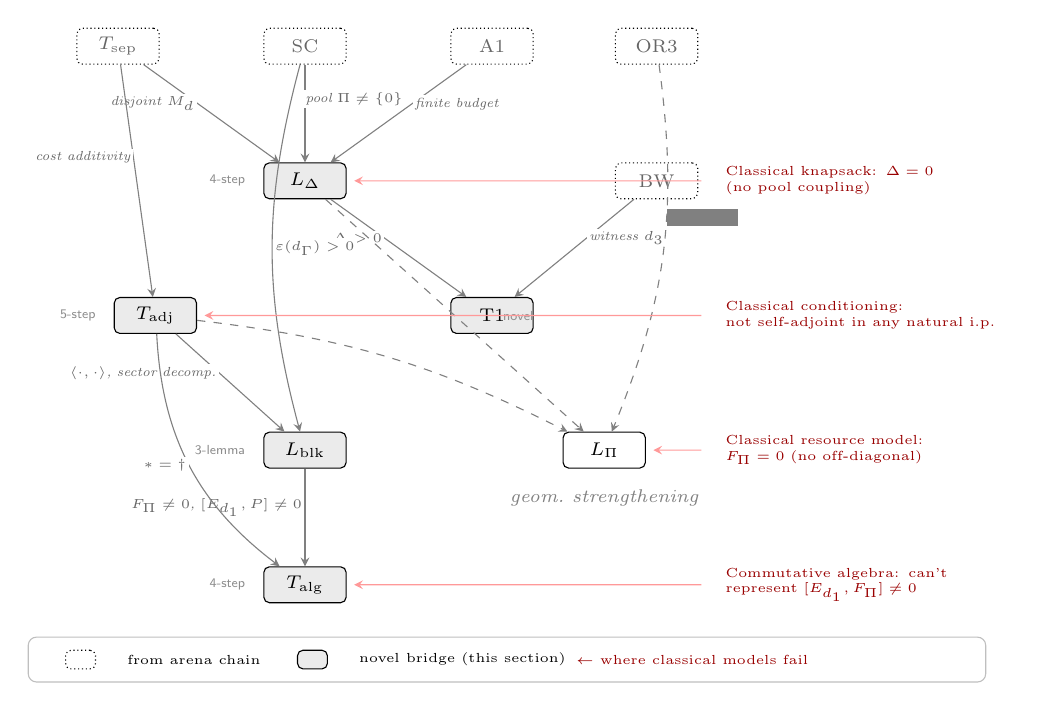
\begin{tikzpicture}[
    scale=0.95, every node/.style={transform shape},
    nd/.style={draw, rounded corners=2pt, minimum height=0.48cm, minimum width=1.1cm, inner sep=2pt, font=\scriptsize},
    prior/.style={nd, densely dotted, text=black!60},
    bridge/.style={nd, fill=black!8},
    lemma/.style={nd},
    arr/.style={->, >=stealth, thin, black!50},
    elabel/.style={font=\tiny\itshape, text=black!60, fill=white, inner sep=1pt},
    badge/.style={font=\tiny, text=black!45, anchor=east},
    cfail/.style={font=\tiny, text=red!60!black, anchor=west, text width=3.8cm, align=left},
]

% ── Prior results (dotted) ──
\node[prior] (Tsep) at (-2.0, 0) {$T_{\mathrm{sep}}$};
\node[prior] (SC) at (0.5, 0) {SC};
\node[prior] (A1) at (3.0, 0) {A1};
\node[prior] (OR3) at (5.2, 0) {OR3};
\node[prior] (BW) at (5.2, -1.8) {BW};

% ── Bridge nodes (shaded) ──
\node[bridge] (LDelta) at (0.5, -1.8) {$L_\Delta$};
\node[bridge] (Tadj) at (-1.5, -3.6) {$T_{\mathrm{adj}}$};
\node[bridge] (T1) at (3.0, -3.6) {T1};
\node[bridge] (Lblk) at (0.5, -5.4) {$L_{\mathrm{blk}}$};
\node[bridge] (Talg) at (0.5, -7.2) {$T_{\mathrm{alg}}$};
\node[lemma] (LPi) at (4.5, -5.4) {$L_\Pi$};
\node[font=\scriptsize\itshape, gray, anchor=north] at (4.5, -5.8) {geom.\ strengthening};

% ── Proof-type badges ──
\node[badge] at ($(LDelta.west)+(-0.12,0)$) {\textsf{4-step}};
\node[badge] at ($(Tadj.west)+(-0.12,0)$) {\textsf{5-step}};
\node[badge] at ($(T1.east)+(0.12,0)$) {\textsf{novel}};
\node[badge] at ($(Lblk.west)+(-0.12,0)$) {\textsf{3-lemma}};
\node[badge] at ($(Talg.west)+(-0.12,0)$) {\textsf{4-step}};

% ── Arrows with edge labels ──
\draw[arr] (Tsep) -- node[elabel, left, pos=0.4] {disjoint $M_d$} (LDelta);
\draw[arr] (SC) -- node[elabel, right=-1pt, pos=0.35] {pool $\Pi \ne \{0\}$} (LDelta);
\draw[arr] (A1) -- node[elabel, right, pos=0.4] {finite budget} (LDelta);

\draw[arr] (Tsep) -- node[elabel, left, pos=0.4] {cost additivity} (Tadj);
\draw[arr] (LDelta) -- node[elabel, left, pos=0.4] {$\Delta > 0$} (T1);
\draw[arr] (BW) -- node[elabel, right, pos=0.4] {witness $d_3$} (T1);

\draw[arr] (Tadj) -- node[elabel, left, pos=0.4] {$\langle\cdot,\cdot\rangle$, sector decomp.} (Lblk);
\draw[arr] (SC) to[bend right=15] node[elabel, right, pos=0.5] {$\varepsilon(d_\Gamma) > 0$} (Lblk);

\draw[arr] (Lblk) -- node[elabel, left, pos=0.4] {$F_\Pi \ne 0$, $[E_{d_1},P]\ne 0$} (Talg);
\draw[arr] (Tadj) to[bend right=25] node[elabel, left, pos=0.5] {$* = \dagger$} (Talg);

\draw[arr, gray, dashed] (LDelta) -- (LPi);
\draw[arr, gray, dashed] (Tadj) to[bend left=10] (LPi);
\draw[arr, gray, dashed] (OR3) to[bend left=15] node[elabel, right, pos=0.4, gray] {finite dim} (LPi);

% ── Classical failure annotations ──
\node[cfail] at (6.0, -1.8) {Classical knapsack: $\Delta = 0$\\(no pool coupling)};
\node[cfail] at (6.0, -3.6) {Classical conditioning:\\not self-adjoint in any natural i.p.};
\node[cfail] at (6.0, -5.4) {Classical resource model:\\$F_\Pi = 0$ (no off-diagonal)};
\node[cfail] at (6.0, -7.2) {Commutative algebra: can't\\represent $[E_{d_1}, F_\Pi] \ne 0$};

\draw[->, >=stealth, thin, red!40] (5.8, -1.8) -- ($(LDelta.east)+(0.1,0)$);
\draw[->, >=stealth, thin, red!40] (5.8, -3.6) -- ($(Tadj.east)+(0.1,0)$);
\draw[->, >=stealth, thin, red!40] (5.8, -5.4) -- ($(LPi.east)+(0.1,0)$);
\draw[->, >=stealth, thin, red!40] (5.8, -7.2) -- ($(Talg.east)+(0.1,0)$);

% ── Legend ──
\draw[black!25, rounded corners=3pt] (-3.2, -8.5) rectangle (9.6, -7.9);
\node[prior, minimum width=0.4cm, minimum height=0.25cm] at (-2.5, -8.2) {};
\node[font=\tiny, anchor=west] at (-2.0, -8.2) {from arena chain};
\node[bridge, minimum width=0.4cm, minimum height=0.25cm] at (0.6, -8.2) {};
\node[font=\tiny, anchor=west] at (1.1, -8.2) {novel bridge (this section)};
\node[font=\tiny, text=red!60!black, anchor=west] at (4.0, -8.2) {$\leftarrow$ where classical models fail};

\end{tikzpicture}
\caption[Bridge chain]{%
\textbf{Bridge chain: from superadditivity to noncommutativity.}
Dotted nodes are results from the arena chain (Figure~\ref{fig:arena_dag});
shaded nodes are the novel steps proved in this section.
Right annotations mark the point at which each class of classical model is excluded.
The inner product and adjoint structure enter at $T_{\mathrm{adj}}$ --- \emph{after} $L_\Delta$ and T1 are proved without them.
}
\label{fig:bridge_dag}
\end{figure}

\medskip
Theorem T1 established that enforcement operations $\mathfrak{E}_d$ on the abstract
state set $\Omega$ are order-dependent.  The next four propositions make explicit
how these maps generate a noncommutative $*$-algebra carrying a positive faithful
state functional.  Together they close the bridge from T1 to the GNS construction
invoked in T2.

\smallskip\noindent\textbf{Algebraic objects and their definitions} (consolidated reference).  The proofs below operate on the following objects, each defined in Section~\ref{sec:defs}; the type signatures are collected in the Formal Specification tables (p.\,\pageref{box:formal_spec}).

\smallskip
\begin{tabular}{@{}p{3.0cm}p{9.5cm}@{}}
\textbf{Object} & \textbf{Definition and location} \\[2pt]
\hline\noalign{\smallskip}
Enforcement operation $E_d$ & Linear idempotent on $S_\Gamma$ with $\mathrm{im}(E_d) = M_d$, $E_d^2 = E_d$ (FD5a, \S\ref{sec:defs}); upgraded to orthogonal projection $\pi_{M_d}$ after $T_{\mathrm{adj}}$ derives the inner product (FD5b). \\[4pt]
Anchor set $M_d$ & Minimal linear subspace of $S_\Gamma$ containing the support of every perturbation in $\mathcal{P}(d)$ (FD3, \S\ref{sec:defs}). \\[4pt]
Enforcement algebra $\mathcal{A}$ & $\mathrm{Alg}_\mathbb{R}(\mathcal{G}) \subseteq \mathrm{End}(V)$, with $\mathcal{G} = \{E_d\} \cup \{E_{\{d_1,d_2\}}\}$; product $=$ composition; identity $= \mathrm{Id}_V$; norm $= \|A\|_{\mathrm{op}} := \sup_{v \ne 0}\|Av\|/\|v\|$ (inherited from $\mathrm{End}(V)$); $*$-involution $G^* := G$ on generators, extended anti-multiplicatively (Definition~\ref{def:enforcement_algebra}, O3). \\[4pt]
Cost symmetry & The property $\omega(E_d A) = \omega(A E_d)$ for the cost functional $\omega(A) = \varepsilon(A)/C$; derived in $T_{\mathrm{adj}}$ from $T_{\mathrm{sep}}$ + K3 (disjoint-support additivity of $\kappa$).  It forces the inner product (Eq.~\ref{eq:canon_ip}) in which $E_d = E_d^\dagger$. \\[4pt]
Positivity/continuity for $*$-involution & None assumed.  $T_{\mathrm{adj}}$ \emph{constructs} the inner product from cost additivity (Step~3) and proves $E_d = E_d^\dagger$ (Step~5) from idempotency + sector orthogonality.  The only inputs are $T_{\mathrm{sep}}$ (disjoint mechanisms, from A1) and K3 (additive $\kappa$ on disjoint supports, from A1's budget accounting). \\
\end{tabular}

\smallskip\noindent The substrate vector space $V = \mathrm{span}_\mathbb{R}(K)$ is finite-dimensional ($\dim V \le n_{\max} + 1$, from OR3); the operator norm and C$^*$-identity are automatic consequences of finite-dimensional $*$-subalgebras of $\mathrm{End}(V)$ (proved inline in ``Why $C^*$,'' \S\ref{sec:operator_bridge}).

The passage from order-dependence on $\Omega$ to a noncommutative operator algebra requires three structural conditions on the enforcement maps.  These are stated explicitly as hypotheses and then verified from the framework's prior results.

\smallskip\noindent\textbf{Hypotheses on the enforcement maps} (verified from prior results):
\textbf{H\textsubscript{aff}}: each $\mathfrak{E}_d$ is affine on the convex set $K$ (from the cost-vector embedding, enforcement acts as a translation in $\mathbb{R}^{|\mathcal{D}|+1}$).
\textbf{H\textsubscript{comp}}: composition is closed on $K \cup \{\bot\}$ (from A1 and OR1).
\textbf{H\textsubscript{cont}}: continuity is automatic since $K$ is finite-dimensional (from OR3 + $L_{\varepsilon^*}$).

\smallskip\noindent\textit{Notation bridge.}  Three notations for enforcement operations appear across the paper, all referring to the same physical object at successively richer levels of mathematical structure: (a) $\mathfrak{e}_d$ (lowercase fraktur) is the abstract partial map $\Omega \to \Omega \cup \{\bot\}$ defined in FD4, acting on the state set; (b) $\mathfrak{E}_d$ (uppercase fraktur) is used interchangeably with $\mathfrak{e}_d$ when the domain is the convex polytope $K = \mathrm{conv}(\varphi(\Omega))$, in particular in the T1 statement and worked example; (c) $E_d$ (uppercase roman) denotes the linear extension of $\mathfrak{E}_d$ to all of $V = \mathrm{span}_\mathbb{R}(K)$, established by Proposition O1 below.  All three refer to the same enforcement operation; the notation signals which mathematical level is in scope.

\smallskip\noindent\textbf{Proposition O1 (Affine extension to linear operators).}
\emph{Each enforcement map $\mathfrak{E}_d: K \to K \cup \{\bot\}$ extends uniquely to a linear operator $E_d \in \mathrm{End}(V)$, where $V = \mathrm{span}_\mathbb{R}(K)$.}

\smallskip\noindent\textbf{Convention ($\bot = 0$).}  The failure symbol $\bot$ is identified with $0 \in V$ under the linear extension.  This is forced: $0$ is the unique element of $V$ that is not in the image of any admissible enforcement path (every $k \in K$ has at least one active distinction, hence nonzero cost-vector embedding), so identifying $\bot$ with $0$ is the only assignment consistent with linearity.  Concretely, $T_{\mathrm{adj}}$ defines $E_d$ as the orthogonal projection onto $M_d \subset S_\Gamma$, which maps all of $\ker(E_d) = M_d^\perp$ to $0$; states that would require budget exceeding $C$ are exactly those whose linear-extension image falls in the $\bot = 0$ locus.  After this identification, $E_d \in \mathrm{End}(V)$ is a total linear map with $\bot$ replaced by its algebraic representative $0$.

\smallskip\noindent\textbf{Proof.}
By H\textsubscript{aff}, each $\mathfrak{E}_d$ is affine on $K$: it acts as a translation in the cost-vector embedding $\varphi: \Omega \to \mathbb{R}^{|\mathcal{D}|+1}$, incrementing the $d$-indicator coordinate from $0$ to $1$ and decrementing the budget coordinate by $\varepsilon(d)/C$.  An affine map on a convex set $K \subset \mathbb{R}^N$ has a unique linear extension to the real span $V = \mathrm{span}_\mathbb{R}(K)$: writing any $v \in V$ as a real linear combination $v = \sum_i \lambda_i k_i$ with $k_i \in K$, define $E_d(v) := \sum_i \lambda_i \mathfrak{E}_d(k_i)$ where $\mathfrak{E}_d(k_i) \in K$ is replaced by $0$ whenever $\mathfrak{E}_d(k_i) = \bot$.  This is well-defined because if $v = \sum_j \mu_j k'_j$ is another representation, the affine condition $\sum_i \lambda_i = \sum_j \mu_j$ ensures consistency; the $\bot = 0$ convention is compatible because $0 \in V$ and linearity is preserved.  Linearity of $E_d$ on $V$ follows immediately: $E_d(\alpha u + \beta v) = \alpha E_d(u) + \beta E_d(v)$ for all $u, v \in V$, $\alpha, \beta \in \mathbb{R}$.  Finiteness: $\dim V \leq N+1 < \infty$ since $V \subseteq \mathbb{R}^{N+1}$ (canonical embedding above; $N = |\mathcal{B}| \leq \lfloor C/\mu^* \rfloor$).  Therefore $E_d \in \mathrm{End}(V)$.  \hfill$\square$

\smallskip\noindent\textbf{Proposition O2 (Distinct enforcement operators).}
\emph{There exist distinctions $a, b \in \mathcal{D}$ such that $E_a \ne E_b$ as operators in $\mathrm{End}(V)$.  Specifically, there exists a state $\sigma_0 \in K$ and a distinction $d_3$ such that $E_{d_3} E_{d_1} \sigma_0 \ne E_{d_3} E_{d_2} \sigma_0$ in $V$.}

\smallskip\noindent\textbf{Proof.}
Take the witness from T1: distinctions $d_1, d_2$ with $\varepsilon(d_1) \ne
\varepsilon(d_2)$ (NT) sharing substrate $\Gamma$ ($\Delta > 0$ by $L_\Delta$),
and a third distinction $d_3$ with $C - \varepsilon(d_1) \ge \varepsilon(d_3)
> C - \varepsilon(d_2)$.  Then:
\begin{align*}
E_{d_3} E_{d_1} \sigma_\emptyset
  &= (\{d_1, d_3\},\; C - \varepsilon(d_1) - \varepsilon(d_3)) \;\in\; K, \\
E_{d_3} E_{d_2} \sigma_\emptyset
  &= 0 \;\in\; V \quad (\text{budget exceeded; } \bot \text{ identified with } 0 \text{ by O1 convention}).
\end{align*}
The first is a nonzero element of $K \subset V$ (it has at least one active distinction and positive residual budget); the second is $0 \in V$.  These are distinct elements of $V$.  Therefore $E_{d_3} E_{d_1} \ne E_{d_3} E_{d_2}$
in $\mathrm{End}(V)$, which implies $E_{d_1} \ne E_{d_2}$ as operators.  \hfill$\square$

\smallskip\noindent\textit{Remark on what O2 establishes.}
O2 shows $E_{d_1} \ne E_{d_2}$ as operators and that the two orderings produce distinguishably different states at the intermediate stage.  The final states $(\{d_1,d_2\},\,C{-}\varepsilon(d_1){-}\varepsilon(d_2){-}\Delta)$ coincide for both orderings — joint enforcement cost is symmetric — so commutativity of the final-state map does not contradict T1.  Algebraic noncommutativity $[E_{d_1},E_{d_2}]\ne 0$ in the $*$-algebra sense is a post-GNS phenomenon, established in T2 and via the explicit commutator in Cor.~\ref{cor:T_alg}.


\smallskip\noindent\textit{Why this is not classical resource accounting.}
Classical resource models---priority queues, inventory systems, Markov chains with resource states, Petri nets---also exhibit order-dependent intermediate states: processing job $A$ before job $B$ leaves a different queue residual than the reverse.  Even a non-abelian classical group like $S_3$ acting on a finite state set produces order-dependent transitions.  Bayesian conditioning is a sharper example: conditioning a probability measure on event $A$ then event $B$ gives a different posterior than conditioning first on $B$ then $A$ (order-dependent); yet the underlying event algebra is the Boolean $\sigma$-algebra on $X$, which is commutative.  So T1's order-dependence and $T_{\mathrm{alg}}$'s non-commutativity of the abstract algebra are not by themselves signatures of quantum mechanics; the inference from order-dependence to a noncommutative operator algebra requires a further argument.  That argument is supplied by OR2 and the following proposition.

\smallskip\noindent\textbf{Classical model exclusion.}  Any classical model with observable algebra $\mathcal{A}_{\mathrm{cl}} = \ell^\infty(X) \cong \mathbb{R}^{|X|}$ is commutative.  Update maps (Bayesian conditioning, coarse-graining) live in $\mathrm{End}(\Delta(X))$, not in $\mathcal{A}_{\mathrm{cl}}$; they cannot satisfy OR2 (elements of $\mathcal{A}$ that are self-adjoint there) while producing T1-type order dependence.  OR2 is the condition classical models fail: it forces the enforcement operators into the observable algebra where commutativity would hold.


\smallskip\noindent\textit{Remark (scope of OR2).}  OR2's role is double: it is the condition that (a)~classical models cannot satisfy while also satisfying T1 (Prop.~CME: if enforcement operators are self-adjoint elements of a commutative algebra, they commute, contradicting order-dependence) and (b)~forces noncommutativity via $T_{\mathrm{alg}}$ when order-dependence is present.  Without OR2, APF's enforcement maps on $\Omega$ are order-dependent (T1) but admit a commutative algebraic description --- exactly as Bayesian conditioning does.  OR2 is the step that crosses the boundary.  It is not a free additional axiom: it follows from the operational requirement that the cost of enforcing $d$ equals the cost of certifying that $d$ holds (maintenance = detection), which is the physical content of the enforcement framework.  The cost functional $\omega(A) = \varepsilon(A)/C$ is symmetric in this sense: $\omega(E_d A) = \omega(A E_d)$ for all $A$ iff $E_d^* = E_d$ under $\omega$, which OR2 declares.

The step that separates APF from all classical resource models is therefore \textbf{OR2 + $L_{\mathrm{blk}}$}.  Once OR2 is in place, the enforcement algebra $\mathcal{A}$ is a finitely-generated real $*$-algebra in which all generators are self-adjoint; and once $L_{\mathrm{blk}}$ establishes that any admissible joint defender exceeds the direct-sum form (i.e., $\Delta > 0$ forces a genuine off-diagonal component $F_\Pi$ into $\mathcal{A}$), the noncommutativity $[E_{d_1}, F_\Pi] \ne 0$ follows by direct computation ($L_{\mathrm{blk}}$(c)).  This is the hypothesis of Wedderburn--Artin (T2a): any finite-dimensional semisimple real $*$-algebra with self-adjoint generators decomposes as $\bigoplus_k M_{n_k}(\mathbb{F}_k)$ over division rings.  The subsequent Frobenius and local-tomography arguments select $\mathbb{F}_k = \mathbb{C}$ and $k = 1$.  Classical resource systems---even non-abelian ones---are not $*$-algebras of self-adjoint observable-algebra elements and cannot receive the Wedderburn--Artin classification.  The transition from classical order-dependence to quantum noncommutativity is localized precisely at OR2 $+$ $L_\Pi$, not at T1.


\begin{tcolorbox}[defbox, title={Linear Structure Provenance: Where Each Piece of Geometry Enters}]
\label{box:provenance}
The bridge proofs ($T_{\mathrm{adj}}$, $L_{\mathrm{blk}}$, $L_\Pi$, $T_{\mathrm{alg}}$) use linear-algebraic operations: inner products, orthogonal projections, block decompositions.  None of these are assumed.  Every piece of linear geometry is \emph{derived} from the resource axioms A1 + MD before it is used.  The following table traces the provenance.

\smallskip
\begin{center}
\small
\begin{tabular}{@{}p{2.8cm}p{2.8cm}p{2.0cm}p{4.5cm}@{}}
\textbf{Structure used} & \textbf{Where derived} & \textbf{From what} & \textbf{Mechanism} \\[2pt]
\hline\noalign{\smallskip}
Convex mixing & OR1 (\S\ref{sec:defs}) & A1 & $C \in \mathbb{R}_{>0}$ is divisible $\Rightarrow$ budget splits proportionally $\Rightarrow$ convex combinations of strategies are admissible \\[4pt]
Finite-dim vector space & $T_{\mathrm{embed}}$ (\S\ref{sec:defs}) & OR1 + $L_{\varepsilon^*}$ & Convex body $K = \mathrm{conv}(\varphi(\Omega)) \subset \mathbb{R}^{N+1}$ with $N \le \lfloor C/\varepsilon^* \rfloor$ \\[4pt]
Sector decomposition & $T_{\mathrm{sep}}$ (\S\ref{sec:defs}) & A1 + FD3/FD4 & Disjoint anchor sets $\Rightarrow$ $S_\Gamma = \bigoplus_d M_d \oplus \Pi$ \\[4pt]
Inner product & $T_{\mathrm{adj}}$ Step~3 & $T_{\mathrm{sep}}$ + K3 & Cross-sector costs vanish $\Rightarrow$ cost-compatible sector-orthogonal bilinear form (Eq.~\ref{eq:canon_ip}); unique up to within-sector normalization \\[4pt]
Orthogonal projections & $T_{\mathrm{adj}}$ Steps~4--5 & FD5a + Step~3 & Idempotent + self-adjoint in the derived inner product $= $ orthogonal projection \\[4pt]
Grassmannian compactness & $L_\Pi$(a) (geometric) & OR3 ($T_{\mathrm{form}}$) & $\dim S_\Gamma < \infty \Rightarrow \mathrm{Gr}(k,n)$ is compact; used in $L_\Pi$ (not on critical path) \\[4pt]
$*$-involution & O3.v & $T_{\mathrm{adj}}$ & $E_d = E_d^\dagger$ for all generators; extended anti-multiplicatively \\[4pt]
Faithful positive state & O4 & Cost functional & $\omega(A) := \varepsilon(A)/C$; positivity + faithfulness from $T_{\mathrm{sep}}$ + $T_{\mathrm{adj}}$ \\
\end{tabular}
\end{center}

\smallskip\noindent\textbf{The entry point of linear structure is OR1} (budget divisibility $\Rightarrow$ convex mixing), which follows from A1's real-valued capacity $C \in \mathbb{R}_{>0}$.  No inner product, no preferred basis, no geometric structure is assumed prior to T$_{\mathrm{adj}}$ Step~3, which \emph{constructs} the inner product from the cost functional.  The formal embedding of enforcement operations into a sequential effect algebra, verifying the Gudder--Greechie and van de Wetering hypotheses from enforcement primitives alone, is given in Appendix~\ref{app:sea}.

\smallskip\noindent\textbf{Non-circularity audit: T$_{\mathrm{adj}}$, $L_{\mathrm{blk}}$, and $L_\Pi$.}  Three results attract the circularity concern; all are clean.

\smallskip\noindent\textit{$T_{\mathrm{adj}}$ (self-adjointness).}  $T_{\mathrm{adj}}$ does not \emph{invoke} an inner product --- it \emph{constructs} one.  Steps~1--2 use only idempotency (FD5a: $E_d^2 = E_d$, from the constitutive definition of enforcement) and the sector decomposition ($T_{\mathrm{sep}}$: $M_d \cap M_{d'} = \{0\}$, from A1 + FD3/FD4).  Step~3 \emph{defines} $\langle u, v \rangle_{S_\Gamma}$ by declaring cross-sector inner products zero (forced by cost additivity of disjoint mechanisms, which is $T_{\mathrm{sep}}$'s content) and choosing any positive-definite form within each sector.  Steps~4--5 then prove $\ker(E_d) = M_d^\perp$ and $E_d = E_d^\dagger$ in the Step~3 inner product.  The derivation order is: cost additivity $\to$ inner product $\to$ self-adjointness.  At no point does $T_{\mathrm{adj}}$ use a result that depends on self-adjointness.

\smallskip\noindent\textit{$L_{\mathrm{blk}}$ (failure of direct-sum realizability).}  $L_{\mathrm{blk}}$ uses only: (a)~the sector decomposition from $T_{\mathrm{sep}}$, (b)~$\varepsilon(d_\Gamma) > 0$ from SC + A1, (c)~the block structure of self-adjoint idempotents.  It does not invoke the Grassmannian, compactness, or any optimization.  Its proof is three short lemmas closing a biconditional.

\smallskip\noindent\textit{$L_\Pi$ (codespace rotation, geometric strengthening).}  $L_\Pi$ does not \emph{presuppose} a rotation --- it \emph{proves} $W \ne M_{d_1} \oplus M_{d_2}$.  Its inputs are: (a)~the $T_{\mathrm{adj}}$ inner product (constructed, not assumed); (b)~$\Delta > 0$ from $L_\Delta$ (proved from A1 + SC + $T_{\mathrm{sep}}$); (c)~Grassmannian compactness (from OR3: $\dim S_\Gamma < \infty$, proved by $T_{\mathrm{form}}$ from A1 + MD + SC).  $L_\Pi$ is not on the critical path; $L_{\mathrm{blk}}$ carries the proof-bearing load.
\end{tcolorbox}


\begin{tcolorbox}[apfbox, title={Theorem $T_{\mathrm{adj}}$ --- Bridge Step 1: $*$-Involution from Cost Symmetry}]
\textit{Cost additivity over disjoint mechanisms forces a sector-orthogonal inner product on the substrate (unique up to within-sector normalization), in which every enforcement operation is an orthogonal projection --- self-adjoint by construction.}

\smallskip\noindent\textbf{Statement.}  Let $d \in \mathcal{D}$ be any enforceable distinction with enforcement mechanism $M_d \subseteq S_\Gamma$ of any dimension $m = \dim(M_d) \ge 1$.  Then the enforcement operation $E_d$ is self-adjoint,
\[
E_d \;=\; E_d^\dagger,
\]
in every cost-compatible inner product on $S_\Gamma$ --- that is, every positive-definite bilinear form satisfying the sector orthogonality forced by cost additivity (Step~3 below).  The self-adjointness conclusion is independent of the within-sector metric choice.  OR2 ($E_d = E_d^\dagger$ for all generators) holds as a theorem of $T_{\mathrm{sep}}$ + cost additivity for \emph{all} distinctions in $\mathcal{D}$, irreducible or degenerate; it is not declared.

\smallskip\noindent\textit{Variables.}
\begin{varlist}
\item $M_d$ --- the enforcement mechanism of $d$: the minimal subspace of $S_\Gamma$ whose configuration carries $d$, of any dimension $m = \dim(M_d) \ge 1$.
\item $E_d$ --- the enforcement operation for $d$: the idempotent map $S_\Gamma \to S_\Gamma$ committing the system to the $d$-active configuration.
\item $\langle \cdot, \cdot \rangle_{S_\Gamma}$ --- any cost-compatible inner product on $S_\Gamma$: sector-orthogonal with respect to the $T_{\mathrm{sep}}$ decomposition, positive-definite within each sector (Step~3 below).
\end{varlist}

\smallskip\noindent\textbf{Depends on.}  $T_{\mathrm{sep}}$ (disjoint anchors $\Leftrightarrow$ separated perturbation classes; \S\ref{sec:defs}), cost additivity (K3 of $\kappa$; Proposition~\ref{prop:meas}), FD5a (algebraic idempotent; \S\ref{sec:defs}).

\smallskip\noindent\textbf{Status.}  \textbf{[Proved]} --- five-step proof below.  The bilinear form is \emph{constructed} in Step~3, not assumed.  \textit{Supplement alignment:} in the Formal Supplement's architecture this theorem is split into a four-lemma chain ($L_{\mathrm{idem}} \to L_\omega \to L_{\mathrm{mc}} \to T_{\mathrm{adj}}$): Step~3 here is Lemma~$L_\omega$ (sector-orthogonal bilinear form, a prior named result in the supplement); Steps~4--5 are $T_{\mathrm{adj}}$ proper.  The mathematical content is identical; the supplement's presentation names the bilinear-form construction as a separate lemma to make the logical dependencies explicit.

\smallskip\noindent\textbf{Proof.}

\textit{Step~1 (Idempotency).}  Enforcing $d$ when $d$ is already active commits no additional capacity and leaves the state unchanged: $E_d(\sigma) = \sigma$ for all $\sigma$ with $d$ active.  Extended by linearity over $S_\Gamma$: $E_d \circ E_d = E_d$.  So $E_d$ is a projection (idempotent linear map).

\textit{Step~2 (Sector decomposition and enforcement generator definition).}  By $T_{\mathrm{sep}}$ (recall: $d_1 \perp d_2$ iff $M_{d_1} \cap M_{d_2} = \{0\}$; proved from A1 in Section~\ref{sec:defs}), $M_d \cap M_{d'} = \{0\}$ for all $d \ne d'$.  The anchor sets are pairwise disjoint but need not exhaust $S_\Gamma$: the substrate pool $\Pi := S_\Gamma \setminus \bigoplus_d M_d$ may be non-empty (it is non-empty whenever the interface carries additional degrees of freedom beyond those assigned to identified distinctions; this is the CL3 condition in $L_\Delta$).  The correct decomposition is therefore:
\[
S_\Gamma \;=\; \Bigl(\bigoplus_d M_d\Bigr) \;\oplus\; \Pi,
\]
where $\Pi$ is the orthogonal complement of all anchor sectors in $S_\Gamma$.  Define the enforcement generator $E_d$ by its action on each component:
\[
E_d\big|_{M_d} = \mathrm{id}, \qquad E_d\big|_{M_{d'}} = 0 \;(d' \ne d), \qquad E_d\big|_{\Pi} = 0.
\]
This is the operational content of ``enforcing $d$'': the mechanism $M_d$ is activated; all other anchor sectors and the pool $\Pi$ are left unchanged.  Then: $E_d^2 = E_d$ (idempotent), $\mathrm{ran}(E_d) = M_d$, $\ker(E_d) = \bigoplus_{d' \ne d} M_{d'} \oplus \Pi$.

\textit{Step~3 (Sector-orthogonal inner product from cost additivity).}  By $T_{\mathrm{sep}}$ and $\kappa_\times = 0$ (no joint-vulnerability for disjoint mechanisms, from the $T_{\mathrm{sep}}$ Corollary), the enforcement cost is exactly additive: $\varepsilon(\{d, d'\}) = \varepsilon(d) + \varepsilon(d')$ for all $d \ne d'$.  Pool degrees of freedom in $\Pi$ carry no direct distinction cost (though they contribute to $c_\Gamma$ in $L_\Delta$).  This additive separation law implies a canonical \emph{sector-orthogonal} inner product on $S_\Gamma$.  For $u = \sum_d u_d + u_\Pi$, $v = \sum_d v_d + v_\Pi$ with $u_d, v_d \in M_d$ and $u_\Pi, v_\Pi \in \Pi$:
\begin{equation}\label{eq:canon_ip}
\langle u, v \rangle_{S_\Gamma} \;:=\; \sum_d \langle u_d, v_d \rangle_{M_d} \;+\; \langle u_\Pi, v_\Pi \rangle_{\Pi},
\end{equation}
where each $\langle \cdot, \cdot \rangle_{M_d}$ is any positive-definite inner product on sector $M_d$ normalized to cost scale, and $\langle \cdot, \cdot \rangle_\Pi$ is any positive-definite inner product on $\Pi$.  Cross-sector terms vanish: $\langle u_d, v_{d'} \rangle = 0$ for $d \ne d'$; $\langle u_d, v_\Pi \rangle = 0$ for all $d$.  \emph{Why cost additivity forces this:}  if $\langle u_d, v_{d'} \rangle \ne 0$ for some $d \ne d'$, then the orthogonal complement of $M_d$ would depend on $M_{d'}$ --- enforcing $d$ (projecting onto $M_d$) would alter the $M_{d'}$-components of the state, coupling the cost of maintaining $d$ to the configuration of $d'$.  This contradicts $T_{\mathrm{sep}}$'s perturbation-class separation: perturbations in $\mathcal{P}(d)$ act within $M_d$ and cannot affect $M_{d'}$ when $M_d \cap M_{d'} = \{0\}$.  Sector orthogonality is the unique inner-product condition that makes $\ker(E_d)$ independent of all other sectors, preserving the cost additivity established by $T_{\mathrm{sep}}$.  What cost additivity pins is the inter-sector orthogonality; the within-sector metric on each $M_d$ is a normalization convention (any positive-definite choice produces the same orthogonal decomposition and the same algebraic structure; the specific normalization is fixed by the budget deployment in Paper~2, analogous to choosing units within each sector).

\emph{Inner-product axiom verification.}  The bilinear form \eqref{eq:canon_ip} satisfies:
(i)~\emph{Bilinearity}: immediate from linearity of each summand $\langle \cdot, \cdot \rangle_{M_d}$ and $\langle \cdot, \cdot \rangle_\Pi$.
(ii)~\emph{Symmetry}: each within-sector form is symmetric by construction (positive-definite real bilinear forms are symmetric).
(iii)~\emph{Positive definiteness}: for any nonzero $v = \sum_d v_d + v_\Pi \in S_\Gamma$, at least one component $v_d$ or $v_\Pi$ is nonzero.  Since each within-sector form is positive definite (by the choice of $\langle \cdot, \cdot \rangle_{M_d}$ and $\langle \cdot, \cdot \rangle_\Pi$), $\langle v, v \rangle_{S_\Gamma} = \sum_d \langle v_d, v_d \rangle_{M_d} + \langle v_\Pi, v_\Pi \rangle_\Pi > 0$.  (Each term is $\ge 0$; at least one is $> 0$.)
(iv)~\emph{Representation independence}: the projection $E_d = \pi_{M_d}$ depends only on which subspace $M_d$ is the range and which is the kernel; the orthogonal decomposition $S_\Gamma = \bigoplus_d M_d \oplus \Pi$ is independent of the within-sector metric choice.  Therefore the $*$-algebra structure ($E_d = E_d^\dagger$, the commutation relations, and all downstream results) is independent of the normalization convention within each sector.

\textit{Step~4 (Kernel is the orthogonal complement).}  By construction \eqref{eq:canon_ip}, $M_d \perp M_{d'}$ for all $d \ne d'$, and $M_d \perp \Pi$ for all $d$.  Therefore
\[
\ker(E_d) = \Bigl(\bigoplus_{d' \ne d} M_{d'}\Bigr) \oplus \Pi \;=\; M_d^\perp.
\]
Hence $E_d$ is the \emph{orthogonal projection} onto $M_d$, for any $\dim(M_d) \ge 1$.

\textit{Step~5 (Self-adjointness).}  Write $u = u_d + u^\perp$, $v = v_d + v^\perp$ with $u_d, v_d \in M_d$ and $u^\perp, v^\perp \in M_d^\perp = (\bigoplus_{d' \ne d} M_{d'}) \oplus \Pi$.  Then $E_d u = u_d$, $E_d v = v_d$, and:
\[
\langle E_d u,\, v \rangle_{S_\Gamma} = \langle u_d,\, v_d \rangle_{M_d}, \qquad
\langle u,\, E_d v \rangle_{S_\Gamma} = \langle u_d,\, v_d \rangle_{M_d},
\]
where the cross terms $\langle u_d, v^\perp\rangle$ and $\langle u^\perp, v_d\rangle$ vanish by Step~4 ($u^\perp, v^\perp \in M_d^\perp$).  Therefore $\langle E_d u, v \rangle_{S_\Gamma} = \langle u, E_d v \rangle_{S_\Gamma}$ for all $u, v \in S_\Gamma$, so $E_d = E_d^\dagger$.  \hfill$\square$

\smallskip\noindent\textbf{Corollary.}  OR2 ($E_d^* = E_d$) is a proved theorem, not an assumption.

\smallskip\noindent\textit{Remark (uniqueness of the inner product).}  What $T_{\mathrm{adj}}$ derives is: (i)~sector orthogonality (forced by cost additivity --- no choice), and (ii)~self-adjointness of all $E_d$ (forced by idempotency + sector orthogonality --- no choice).  What it does \emph{not} uniquely determine is the within-sector metric on $M_d$ when $\dim(M_d) > 1$.  For irreducible distinctions ($\dim(M_d) = 1$), the metric within $M_d$ is a single positive number, fixed by the cost normalization $\varepsilon(d) = \varepsilon^*$; the inner product is therefore unique.  For composite distinctions ($\dim(M_d) > 1$), the metric within $M_d$ is a positive-definite form on $\mathbb{R}^m$, which has $m(m+1)/2 - 1$ degrees of freedom.  This freedom does not affect any downstream result: the projection $E_d = \pi_{M_d}$ is the same for any positive-definite within-sector metric, and the $*$-algebra structure, the GNS construction, and Wedderburn--Artin all depend only on the orthogonal decomposition and the projection structure.  The specific within-sector normalization is fixed by the budget deployment in Paper~2 (analogous to choosing units within each gauge sector).

\smallskip\noindent\textit{Remark (relation to the L\"uders adjoint and sequential effect algebras).}
$T_{\mathrm{adj}}$'s cost-derived adjoint is the L\"uders adjoint.  Precisely: since $E_d$ is an orthogonal projection ($E_d^2 = E_d$, $E_d = E_d^\dagger$, from Steps~1 and~5), the sequential enforcement of $d_1$ conditional on $d_2$ is the map $\rho \mapsto E_{d_1}^{1/2}\, E_{d_2}\, E_{d_1}^{1/2} = E_{d_1}\, E_{d_2}\, E_{d_1}$ (since $E_{d_1}^{1/2} = E_{d_1}$ for a projection).  This is exactly the L\"uders update rule $a \circ b := a^{1/2}\, b\, a^{1/2}$ applied to enforcement projections.  The reduction is not a special condition --- it is the generic case after $T_{\mathrm{adj}}$, because every enforcement generator is a self-adjoint idempotent (hence a projection), and $P^{1/2} = P$ for any projection $P$.  For general elements $A, B \in \mathcal{A}$ that are \emph{not} projections (e.g., off-diagonal operators like $F_\Pi$), the sequential product is $A^{1/2}\, B\, A^{1/2}$ with $A^{1/2}$ computed via the functional calculus on $\mathrm{End}(V)$ --- well-defined since $\dim V < \infty$ (OR3).

This is the precise connection to Gudder's framework~\cite{GudderGreechie2002}.  Appendix~\ref{app:sea} (Proposition~\ref{prop:sea}) verifies that the enforcement operations form a sequential effect algebra (SEA), and Proposition~\ref{prop:gg_hyps} verifies conditions (GG1)--(GG3) of the Gudder--Greechie representation theorem.  That theorem then delivers a faithful SEA homomorphism $\phi: E \to \mathcal{B}(\mathcal{H})$ with $\phi(a \mid b) = \phi(a)^{1/2}\,\phi(b)\,\phi(a)^{1/2}$ (the L\"uders product).  The logical order is: $T_{\mathrm{adj}}$ \emph{derives} the self-adjoint-projection structure from cost symmetry; Gudder--Greechie then confirms that this derived structure admits a Hilbert-space representation in which the sequential product is automatically the L\"uders product.  Neither the L\"uders rule nor the SEA axioms are assumed; both are consequences of cost additivity and idempotency.

\smallskip\noindent\textbf{Corollary (Diagonal subalgebra is commutative).}\label{cor:Adiag}
The sector projections $\{E_d : d \in \mathcal{D}\}$ generate a commutative real $*$-subalgebra
\[
\mathcal{A}_{\mathrm{diag}} \;:=\; \mathrm{span}_{\mathbb{R}}\{E_d : d \in \mathcal{D}\} \;\cong\; \mathbb{R}^{|\mathcal{D}|}.
\]
\textit{Proof.}  By Step~2 of $T_{\mathrm{adj}}$, $E_d|_{M_{d'}} = 0$ for all $d \ne d'$ and $E_d|_\Pi = 0$.  Therefore for any $v \in S_\Gamma$:
\[
E_{d_1}\bigl(E_{d_2}(v)\bigr) = E_{d_1}(v_{d_2}) = 0
\qquad\text{and}\qquad
E_{d_2}\bigl(E_{d_1}(v)\bigr) = E_{d_2}(v_{d_1}) = 0,
\]
so $E_{d_1} E_{d_2} = 0 = E_{d_2} E_{d_1}$ and $[E_{d_1}, E_{d_2}] = 0$ for all pairs $d_1 \ne d_2$.
The subalgebra spanned by orthogonal projections with pairwise-zero products is isomorphic to $\mathbb{R}^{|\mathcal{D}|}$.  \hfill$\square$

\coderef{check\_T\_adj}{paper1.py}\,%
\hspace{1em}\textit{(also verified in \texttt{supplement.py})}
\smallskip\noindent\textit{Supplement cross-reference.}  The Formal Supplement (Appendix~J; \texttt{check\_T\_adj} in \texttt{supplement.py}) verifies this theorem against the four-lemma chain.  The five steps above are the Paper~1 self-contained presentation; the supplement's $L_\omega$ lemma (sector-orthogonal bilinear form) corresponds to Step~3, and $T_{\mathrm{adj}}$ proper to Steps~4--5.  Both verify the same result by the same argument.
\end{tcolorbox}

\smallskip\noindent\textit{Remark (scope of $\mathcal{A}_{\mathrm{diag}}$ and the full algebra).}
The commutativity of $\mathcal{A}_{\mathrm{diag}}$ is the correct algebraic signature of the classical regime: when each distinction is enforced independently, the observable algebra is diagonal.  The critical algebraic obstruction is not ``rotation'' but \emph{failure of direct-sum realizability}: if the joint defense of $d_1$ and $d_2$ were realizable entirely inside $M_{d_1} \oplus M_{d_2}$, the cost would be additive.  Positive excess cost therefore means that every admissible joint defender must carry nontrivial support in the pooled sector $\Pi$.  Noncommutativity is the operator-algebraic certificate of that forced pooled support.

\begin{tcolorbox}[defbox, title={Definition: Direct-Sum Realizability}]
\label{def:ds_realizable}
Let $S_\Gamma = M_{d_1} \oplus M_{d_2} \oplus \Pi$ be the sector decomposition from $T_{\mathrm{adj}}$.  A self-adjoint idempotent joint defender $P$ for $\{d_1, d_2\}$ is \emph{direct-sum realizable} if $\mathrm{supp}(P) \subseteq M_{d_1} \oplus M_{d_2}$ --- equivalently, $P$ has no required support in $\Pi$.
\end{tcolorbox}

\begin{tcolorbox}[apfbox, title={Theorem $L_{\mathrm{blk}}$ --- Excess Cost and Direct-Sum Realizability}]
\label{lem:L_blk}

\textit{Positive excess cost is equivalent to failure of direct-sum realizability of joint defense.  This biconditional is the conceptual center of the bridge from superadditivity to noncommutativity.}

\smallskip\noindent\textbf{Statement.}  Let $S_\Gamma = M_{d_1} \oplus M_{d_2} \oplus \Pi$ (from $T_{\mathrm{sep}}$ + CL3).  The following are equivalent:
\begin{enumerate}[nosep,leftmargin=2em,itemsep=2pt,label=(\roman*)]
\item The joint excess cost vanishes: $\Delta(d_1,d_2) = 0$.
\item There exists an admissible self-adjoint idempotent joint defender $P$ with $\mathrm{supp}(P) \subseteq M_{d_1} \oplus M_{d_2}$ (direct-sum realizable).
\item No positive-cost pooled distinction $d_\Gamma$ with $M_{d_\Gamma} \subseteq \Pi$ is jointly required for defense.
\end{enumerate}
Equivalently: $\Delta(d_1, d_2) > 0$ if and only if \emph{every} admissible self-adjoint idempotent joint defender requires nontrivial $\Pi$-support.

\smallskip\noindent\textbf{Depends on.}  $L_\Delta$ (superadditivity from substrate integrity), $T_{\mathrm{sep}}$ (sector decomposition), SC (every nonzero direction anchors a distinction), A1 ($\varepsilon(d_\Gamma) > 0$), $T_{\mathrm{adj}}$ (self-adjoint projections from cost additivity).

\smallskip\noindent\textbf{Status.}  \textbf{[Proved]} --- three lemmas, each 2--4 lines, no topology or optimization.

\smallskip\noindent\textbf{Proof.}  Three lemmas establish the three implications; together they close the equivalence.

\medskip\noindent\textit{Lemma 1 (Pooled-distinction characterization of excess).}
If $\Delta(d_1,d_2) > 0$, then by $L_\Delta$ and SC there exists a substrate-integrity distinction $d_\Gamma$ with $M_{d_\Gamma} \subseteq \Pi$ and $\varepsilon(d_\Gamma) > 0$: the superadditive surplus is the cost of defending the pool.  Conversely, if no positive-cost distinction has its anchor in $\Pi$, then $\Pi$ contributes no defense requirement, the joint cost is $\varepsilon(d_1) + \varepsilon(d_2)$ (additive over disjoint mechanisms by $T_{\mathrm{sep}}$), and $\Delta = 0$.  This establishes (i) $\Leftrightarrow$ (iii).

\medskip\noindent\textit{Lemma 2 (Direct-sum support cannot defend a pooled distinction).}
Let $P$ be a self-adjoint idempotent with $\mathrm{supp}(P) \subseteq M_{d_1} \oplus M_{d_2}$.  Then $P|_\Pi = 0$, so $P|_{M_{d_\Gamma}} = 0$ for any $M_{d_\Gamma} \subseteq \Pi$.  Such a $P$ cannot defend any distinction whose anchor lies in $\Pi$.  Therefore: (ii) implies (iii) (contrapositively: a positive-cost pooled distinction forbids direct-sum realizability).

\medskip\noindent\textit{Lemma 3 (Additive case gives a block-supported defender).}
If no positive-cost pooled distinction in $\Pi$ is jointly required (condition (iii)), then the direct-sum projector $P_{\mathrm{ds}} := E_{d_1} + E_{d_2}$ is an admissible self-adjoint idempotent joint defender: it defends $d_1$ and $d_2$ by construction ($E_{d_i}|_{M_{d_i}} = \mathrm{id}$), and no additional defense in $\Pi$ is needed since no positive-cost distinction has its anchor there.  Therefore (iii) implies (ii).

\medskip\noindent\textit{Closing the equivalence.}  (i) $\Leftrightarrow$ (iii) by Lemma~1.  (iii) $\Rightarrow$ (ii) by Lemma~3.  (ii) $\Rightarrow$ (iii) by Lemma~2 (contrapositive).  Therefore (i) $\Leftrightarrow$ (ii) $\Leftrightarrow$ (iii).

Contrapositively: $\Delta > 0$ iff every admissible joint defender requires nontrivial $\Pi$-support.  \hfill$\square$

\medskip\noindent\textbf{Corollary (Nonzero commutator witness).}  If $\Delta(d_1,d_2) > 0$, then for any admissible joint defender $P$:
\begin{enumerate}[nosep,leftmargin=2em,itemsep=2pt,label=(\alph*)]
\item $F_\Pi := P - E_{d_1} - E_{d_2} \ne 0$ (failure of direct-sum form).
\item There exists $v \in M_{d_1}$ with $Pv = v + \pi_v$, $\pi_v \in \Pi \setminus \{0\}$.
\item $[E_{d_1}, P]\,v = -\pi_v \ne 0$.
\end{enumerate}
\textit{Proof of (b).}  Since $P$ has nontrivial $\Pi$-support (theorem) and defends $d_1$ ($P|_{M_{d_1}}$ injective), if $Pv \in M_{d_1}$ for all $v \in M_{d_1}$ then $P|_{M_{d_1}} = E_{d_1}|_{M_{d_1}}$, $P|_{M_{d_2}} = E_{d_2}|_{M_{d_2}}$, and $P|_\Pi = 0$ by idempotency --- contradicting nontrivial $\Pi$-support.  So some $v \in M_{d_1}$ has $\pi_v \ne 0$.

\textit{Proof of (c).}  Expand the commutator using $E_{d_1}(v) = v$ (since $v \in M_{d_1}$ and $E_{d_1}|_{M_{d_1}} = \mathrm{id}$) and $E_{d_1}(\pi_v) = 0$ (since $\pi_v \in \Pi \subseteq \ker(E_{d_1})$, which holds because $E_{d_1}|_\Pi = 0$ by $T_{\mathrm{sep}}$'s sector definition, Step~2 of $T_{\mathrm{adj}}$):
\[
[E_{d_1}, P]\,v \;=\; E_{d_1}(Pv) - P(E_{d_1}v) \;=\; E_{d_1}(v + \pi_v) - P(v) \;=\; \bigl(E_{d_1}(v) + E_{d_1}(\pi_v)\bigr) - (v + \pi_v) \;=\; (v + 0) - (v + \pi_v) \;=\; -\pi_v \;\ne\; 0.
\]
\hfill$\square$
\end{tcolorbox}

\smallskip\noindent\textit{What $L_{\mathrm{blk}}$ achieves.}  The biconditional establishes the bridge from superadditivity to noncommutativity in three short lemmas, each 2--4 lines, without invoking the Grassmannian, compactness, minimizer existence, or ``codespace rotation.''  The only inputs are the sector decomposition ($T_{\mathrm{sep}}$), the characterization of excess cost ($L_\Delta$), and the block structure of self-adjoint idempotents.  \emph{This is the shortest path from $L_\Delta$ to $[E_{d_1}, P] \ne 0$.}  The converse direction (Lemma~3) is what makes it a biconditional: $\Delta = 0$ is not merely consistent with block-diagonal defense --- it \emph{guarantees} it.

\medskip\noindent The following lemma provides a geometric strengthening: not only must some admissible defender have a $\Pi$-component, but the \emph{cost-minimizing} one tilts by a specific angle determined by $\Delta$.  This geometric picture (Figure~\ref{fig:codespace_rotation}) is the physical intuition behind the algebra; $L_{\mathrm{blk}}$ above is the proof-carrying step.

\begin{tcolorbox}[apfbox, title={Lemma $L_\Pi$ --- Geometric Strengthening: Codespace Rotation}]
\label{lem:L_Pi}
\textit{The cost-minimizing admissible joint defender is an orthogonal projection onto a subspace $W \ne M_{d_1} \oplus M_{d_2}$, tilted into $\Pi$ by the substrate-integrity cost $\Delta > 0$.}

\smallskip\noindent\textbf{Statement.}  Under the hypotheses of $L_{\mathrm{blk}}$, the minimum-cost admissible joint-defense projection $\pi_{W_*}$ satisfies:
\begin{enumerate}[nosep,leftmargin=2em,itemsep=2pt,label=(\alph*)]
\item $W_*$ exists (the infimum cost is attained or approached to within $\epsilon$ for any $\epsilon > 0$).
\item $W_* \ne M_{d_1} \oplus M_{d_2}$ (by $L_{\mathrm{blk}}$(a)).
\item $\dim W_* = \dim(M_{d_1} \oplus M_{d_2})$ (dimension minimality: cost increases strictly with dimension).
\item $M_{d_i} \cap W_*^\perp = \{0\}$ for $i = 1,2$ (non-deactivation).
\end{enumerate}

\smallskip\noindent\textbf{Depends on.}  $L_{\mathrm{blk}}$, $T_{\mathrm{adj}}$ (cost-compatible inner product), OR3 ($\dim S_\Gamma < \infty$).

\smallskip\noindent\textbf{Status.}  \textbf{[Proved]} --- geometric refinement of $L_{\mathrm{blk}}$; not on the critical path.

\smallskip\noindent\textbf{Proof sketch.}  (a) The cost functional $\omega(\pi_W) = \mathrm{tr}(\rho\,\pi_W)$ increases strictly with $\dim W$ (since $\rho$ is positive definite, O4), so the minimizer has the smallest feasible dimension.  At fixed dimension, $\mathrm{Gr}(k,n)$ is compact and $\omega$ is continuous; the infimum on the closure of the feasible set is attained (if the boundary point fails injectivity by a rank-one drop, a perturbation of arbitrarily small cost restores feasibility).  (b) follows from $L_{\mathrm{blk}}$(a).  (c) follows from (a): $\dim W_* = \dim U$ since adding a $\Pi$-direction while maintaining feasibility requires dropping a sector direction (otherwise $\dim W_* > \dim U$ and cost is higher).  (d) follows from the defense requirement: if $M_{d_1} \cap W_*^\perp \ne \{0\}$, an irreducible distinction $d_v$ with $\varepsilon(d_v) > 0$ (SC) is undefended, contradicting feasibility.  \hfill$\square$
\end{tcolorbox}

\smallskip\noindent\textit{Summary ($L_{\mathrm{blk}} \to$ noncommutativity in one paragraph).}  Because any operator supported only on $M_{d_1} \oplus M_{d_2}$ annihilates $\Pi$ and therefore fails to defend $d_\Gamma$ ($L_{\mathrm{blk}}$(a)), any admissible self-adjoint idempotent joint defender $P$ must have a nonzero $\Pi$-linked component ($L_{\mathrm{blk}}$(b)).  The explicit commutator witness $[E_{d_1}, P]\,v = -\pi_v \ne 0$ ($L_{\mathrm{blk}}$(c)) gives noncommutativity directly, in three lines of linear algebra, with no optimization, no topology, and no ``rotation'' language required.  The geometric strengthening ($L_\Pi$) shows that the cost-minimizing such $P$ tilts by an angle determined by $\Delta$ (Figure~\ref{fig:codespace_rotation}), providing physical intuition for the algebraic fact.

\begin{figure}[ht]
\centering
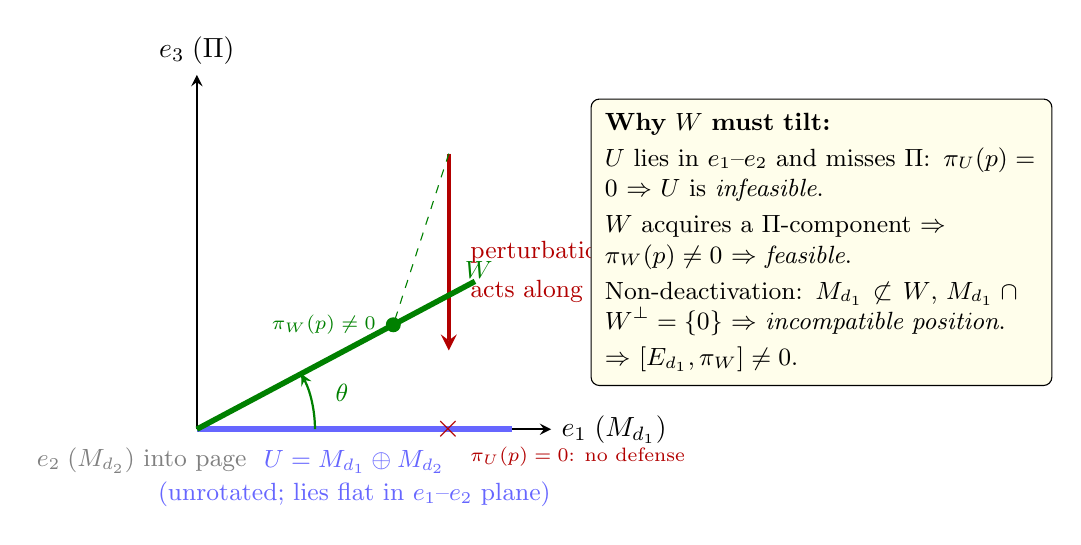
\begin{tikzpicture}[scale=1.0,
    >=stealth,
    axis/.style={thick, ->},
    vec/.style={very thick, ->},
]

% Axes
\draw[axis] (0,0) -- (4.5,0) node[right] {$e_1\;(M_{d_1})$};
\draw[axis] (0,0) -- (0,4.5) node[above] {$e_3\;(\Pi)$};
\node[font=\small, gray] at (-0.7, -0.4) {$e_2\;(M_{d_2})$ into page};

% --- Unrotated codespace U
\draw[very thick, blue!60, line width=2pt] (0,0) -- (4,0);
\node[blue!60, font=\small\bfseries, anchor=north] at (2.0, -0.15) {$U = M_{d_1} \oplus M_{d_2}$};
\node[blue!60, font=\small, anchor=north] at (2.0, -0.55) {(unrotated; lies flat in $e_1$--$e_2$ plane)};

% --- Pool perturbation along e3
\draw[vec, red!70!black, line width=1.5pt] (3.2, 3.5) -- (3.2, 1.0);
\node[red!70!black, font=\small, anchor=west] at (3.35, 2.25) {perturbation $p \in \mathcal{P}(d_\Gamma)$};
\node[red!70!black, font=\small, anchor=west] at (3.35, 1.75) {acts along $\Pi$};

% X mark
\node[red!70!black, font=\large\bfseries] at (3.2, 0.0) {$\times$};
\node[red!70!black, font=\scriptsize, anchor=north west] at (3.35, -0.1) {$\pi_U(p) = 0$: no defense};

% --- Rotated codespace W
\def\tiltangle{28}
\draw[very thick, green!50!black, line width=2pt] (0,0) -- ({4*cos(\tiltangle)},{4*sin(\tiltangle)});
\node[green!50!black, font=\small\bfseries, anchor=south west] at ({3.6*cos(\tiltangle)+0.1},{3.6*sin(\tiltangle)+0.1}) {$W$};

% Tilt angle arc
\draw[thick, green!50!black, ->] (1.5,0) arc[start angle=0, end angle=\tiltangle, radius=1.5];
\node[green!50!black, font=\small] at ({1.9*cos(\tiltangle/2)},{1.9*sin(\tiltangle/2)}) {$\theta$};

% W intercepts perturbation
\draw[dashed, green!50!black, thin] (3.2, 3.5) -- ({3.2*cos(\tiltangle)*cos(\tiltangle)}, {3.2*cos(\tiltangle)*sin(\tiltangle)});
\filldraw[green!50!black] ({3.2*cos(\tiltangle)*cos(\tiltangle)}, {3.2*cos(\tiltangle)*sin(\tiltangle)}) circle (2.5pt);
\node[green!50!black, font=\scriptsize, anchor=east] at ({3.2*cos(\tiltangle)*cos(\tiltangle)-0.1}, {3.2*cos(\tiltangle)*sin(\tiltangle)}) {$\pi_W(p) \ne 0$};

% Annotation box
\node[draw, rounded corners=3pt, fill=yellow!8, inner sep=5pt, font=\small, text width=5.5cm, anchor=north west] at (5.0, 4.2) {%
\textbf{Why $W$ must tilt:}\\[2pt]
$U$ lies in $e_1$--$e_2$ and misses $\Pi$: $\pi_U(p) = 0$ $\Rightarrow$ $U$ is \emph{infeasible}.\\[2pt]
$W$ acquires a $\Pi$-component $\Rightarrow$ $\pi_W(p) \ne 0$ $\Rightarrow$ \emph{feasible}.\\[2pt]
Non-deactivation: $M_{d_1} \not\subset W$, $M_{d_1} \cap W^\perp = \{0\}$ $\Rightarrow$ \emph{incompatible position}.\\[2pt]
$\Rightarrow$ $[E_{d_1}, \pi_W] \ne 0$.
};

\end{tikzpicture}
\caption[Codespace rotation in the $\mathbb{R}^3$ minimal example]{%
\textbf{Codespace rotation ($L_\Pi$) in the $\mathbb{R}^3$ minimal example.}
Both $U$ and $W$ are 2-planes in $\mathbb{R}^3$; this figure shows the cross-section in the $e_1$--$e_3$ plane (the $e_2$ axis, carrying $M_{d_2}$, points into the page, so each 2-plane appears as a line in this slice).
\textbf{Blue:} the unrotated codespace $U = M_{d_1} \oplus M_{d_2}$ (the $e_1$--$e_2$ plane) misses $\Pi$ entirely ($\pi_U(p) = 0$; \emph{infeasible}: fails the $d_\Gamma$ defense constraint).
\textbf{Green:} the rotated codespace $W$ tilts by angle $\theta$ into $\Pi$, intercepting pool perturbations ($\pi_W(p) \ne 0$; \emph{feasible}).
Noncommutativity follows from incompatible position: $M_{d_1} \not\subset W$ (by the tilt) and $M_{d_1} \cap W^\perp = \{0\}$ (non-deactivation), so $E_{d_1}$ and $\pi_W$ are orthogonal projections onto subspaces in incompatible position; by the projection-algebra lemma, $[E_{d_1}, \pi_W] \ne 0$.
The off-diagonal remainder $F_\Pi := \pi_W - E_{d_1} - E_{d_2} \ne 0$ is the witness of the tilt.
}
\label{fig:codespace_rotation}
\end{figure}

\begin{tcolorbox}[defbox, title={Definition FD6: Joint Enforcement Operation (from $L_\Pi$)}]
\label{def:FD6}
\textbf{Definition.}  Let $d_1, d_2 \in \mathcal{D}$ be co-located distinctions at interface $\Gamma$ with $\Delta(d_1,d_2) > 0$ (from $L_\Delta$).  The \emph{joint enforcement operation} is the orthogonal projection
\[
E_{\{d_1,d_2\}} \;:=\; \pi_W \;:\; S_\Gamma \;\longrightarrow\; S_\Gamma,
\]
where $W \subset S_\Gamma$ is the \emph{joint defense codespace} produced by Lemma~$L_\Pi$: the minimum-cost subspace that simultaneously defends $d_1$, $d_2$, and the substrate-integrity distinction $d_\Gamma$.  By $L_\Pi$(a--b), $W$ exists and $\pi_W$ is the optimal defense; by $L_\Pi$(c), $W \ne M_{d_1} \oplus M_{d_2}$; by $L_\Pi$(d), neither mechanism sector is annihilated.

\smallskip\noindent\textit{Operational content.}  Joint defense against the full perturbation class $\mathcal{P}(\{d_1,d_2\})$ --- which includes cross-sector perturbations that target the substrate integrity distinction $d_\Gamma$ --- requires a defense codespace $W$ that is \emph{rotated} relative to the bare sector decomposition $M_{d_1} \oplus M_{d_2}$ ($L_\Pi$(c)).  The rotation encodes both distinctions into a joint subspace that intercepts cross-sector attacks; this is the enforcement-theoretic analogue of quantum error-correction encoding, where the logical codespace is rotated relative to the physical subsystem decomposition.

\smallskip\noindent\textbf{Properties} (all derived from $L_\Pi$):
\begin{enumerate}[nosep,leftmargin=2em,itemsep=3pt,label=(\alph*)]
  \item $E_{\{d_1,d_2\}}^2 = E_{\{d_1,d_2\}}$ and $E_{\{d_1,d_2\}}^\dagger = E_{\{d_1,d_2\}}$: orthogonal projection ($L_\Pi$(b)).
  \item $\omega(E_{\{d_1,d_2\}}) = \varepsilon(\{d_1,d_2\})/C = (\varepsilon(d_1)+\varepsilon(d_2)+\Delta)/C$.
  \item $W \ne M_{d_1} \oplus M_{d_2}$ ($L_\Pi$(c): rotation forced by $\Delta > 0$).
  \item $M_{d_i} \not\subset W$ for some $i \in \{1,2\}$ (consequence of (c) and $\dim W$ minimality).
  \item $M_{d_1} \cap W^\perp = \{0\}$ and $M_{d_2} \cap W^\perp = \{0\}$ ($L_\Pi$(d): non-deactivation).
\end{enumerate}

\smallskip\noindent Properties (a)--(b) and (c)--(e) are proved in Lemma~$L_\Pi$ above.  The incompatibility consequence follows immediately:

\smallskip\noindent\textit{Incompatibility (combining (d) and (e)).}  By FD6(d), WLOG $M_{d_1} \not\subset W$, so $M_{d_1} \cap W \subsetneq M_{d_1}$ (proper subspace).  By FD6(e), $M_{d_1} \cap W^\perp = \{0\}$.  Therefore $(M_{d_1} \cap W) \oplus (M_{d_1} \cap W^\perp) = (M_{d_1} \cap W) \oplus \{0\} = M_{d_1} \cap W \subsetneq M_{d_1}$.  Since $M_{d_1} \ne (M_{d_1} \cap W) \oplus (M_{d_1} \cap W^\perp)$, the subspaces $M_{d_1}$ and $W$ are \emph{incompatible}.  By the standard projection-algebra theorem (two orthogonal projections $P, Q$ commute iff $\mathrm{ran}(P) = (\mathrm{ran}(P) \cap \mathrm{ran}(Q)) \oplus (\mathrm{ran}(P) \cap \mathrm{ran}(Q)^\perp)$), this gives $[\pi_{M_{d_1}}, \pi_W] \ne 0$, i.e., $[E_{d_1}, E_{\{d_1,d_2\}}] \ne 0$.  This argument works uniformly for all $\dim(M_{d_1}) \ge 1$.

\smallskip\noindent\textit{Minimal example (representation-free: uses only the derived real inner-product space; no Hilbert space or complex numbers invoked).}  $S_\Gamma = \mathbb{R}^3$, $M_{d_1} = \mathrm{span}\{e_1\}$, $M_{d_2} = \mathrm{span}\{e_2\}$, $\Pi = \mathrm{span}\{e_3\}$.  Take $W = \mathrm{span}\{(\cos\theta,\, 0,\, \sin\theta),\; (0,1,0)\}$ for $\theta \ne 0$.  Then $\pi_W \ne E_{d_1}+E_{d_2}$ and $[E_{d_1}, \pi_W] \ne 0$; the algebra $\mathcal{A} = \mathrm{Alg}_\mathbb{R}\{E_{d_1}, E_{d_2}, \pi_W\} \cong M_2(\mathbb{R}) \oplus \mathbb{R}$, which is semisimple and noncommutative.  The tilt angle $\theta$ parametrizes the superadditive surplus (Figure~\ref{fig:codespace_rotation}).

\smallskip\noindent\textit{Remark (FD6 as enforcement-theoretic error correction).}  The joint defense codespace $W$ has exactly the structure of a quantum error-correcting code, and the correspondence is not a metaphor --- it is a mathematical identity at the operator-algebra level.

\smallskip\noindent
\small
\begin{tabular}{@{}p{3.8cm}p{4.5cm}l@{}}
\textbf{APF (FD6)} & \textbf{QEC (Knill--Laflamme)} & \textbf{Status} \\[2pt]
\hline\\[-6pt]
Bare sectors $M_{d_1}, M_{d_2}$ & Logical subsystems & FD3 \\[2pt]
Pool $\Pi$ & Syndrome / ancilla space & $T_{\mathrm{adj}}$ Step~2 \\[2pt]
Joint defense codespace $W$ & Encoded logical codespace & FD6 \\[2pt]
$\pi_W$ (projection onto $W$) & Encoding + recovery operation & FD6 \\[2pt]
$W \ne M_{d_1} \oplus M_{d_2}$ (rotation) & Coherent encoding (non-classical) & FD6(c) \\[2pt]
Cross-sector perturbations $\mathcal{P}_\Gamma$ & Error operators (bit-flip, phase-flip, correlated) & P3 \\[2pt]
$\Delta > 0$ (superadditive surplus) & Error-correction overhead & $L_\Delta$ \\[2pt]
Non-deactivation (e) & Code detects all single-sector errors & FD6(e) \\[2pt]
\end{tabular}

\smallskip\noindent The standard logical order in physics runs: \emph{quantum mechanics exists} $\to$ \emph{noncommutative algebras} $\to$ \emph{quantum error correction is possible} (Knill--Laflamme~\cite{NielsenChuang2000}).  The APF derivation reverses this.  A1 forces $\Delta > 0$ ($L_\Delta$); defending the substrate-integrity distinction $d_\Gamma$ renders the direct-sum codespace $U$ infeasible; any feasible minimizer $W$ must acquire a $\Pi$-component, placing $W$ in incompatible position with the sector projections (FD6(d,e)); incompatible orthogonal projections do not commute ($T_{\mathrm{alg}}$).  In this derivation, \emph{the feasibility constraint of defending the shared pool under finite budget is what forces the codespace into incompatible position, and incompatibility is what generates noncommutativity}.  Error correction comes before quantum mechanics in the logical order, not after.  The enforcement-theoretic origin of quantum structure is, at its core, an error-correction argument: nature is forced to encode co-located information coherently because incoherent encoding (the unrotated codespace $M_{d_1} \oplus M_{d_2}$) is infeasible for the full perturbation class.
\end{tcolorbox}

\begin{tcolorbox}[apfbox, title={Corollary of $L_\Pi$ (Joint Enforcement is Not Diagonal)}]
\label{cor:L_Pi_nondiag}
\textit{The joint enforcement generator cannot live in the commutative diagonal subalgebra: superadditivity forces an off-diagonal remainder that does not commute with the sector projections.}

\smallskip\noindent\textbf{Statement.}  Let $d_1, d_2 \in \mathcal{D}$ be co-located distinctions with $\Delta(d_1,d_2) > 0$ (from $L_\Delta$).  Then:
\begin{enumerate}[nosep,leftmargin=2em,itemsep=3pt,label=(\arabic*)]
  \item The joint enforcement generator $E_{\{d_1,d_2\}} \notin \mathcal{A}_{\mathrm{diag}}$.
  \item The off-diagonal remainder $F_\Pi := E_{\{d_1,d_2\}} - E_{d_1} - E_{d_2}$ satisfies $F_\Pi \ne 0$, $F_\Pi \notin \mathcal{A}_{\mathrm{diag}}$, and $F_\Pi^* = F_\Pi$.
  \item $[E_{d_i}, F_\Pi] \ne 0$ for some $i \in \{1,2\}$: the joint defense codespace $W$ is incompatible with at least one bare sector $M_{d_i}$.
\end{enumerate}

\smallskip\noindent\textit{Variables.}
\begin{varlist}
\item $E_{\{d_1,d_2\}} = \pi_W$ --- the joint enforcement generator (FD6): the orthogonal projection onto the joint defense codespace $W$, with $\dim W = \dim(M_{d_1})+\dim(M_{d_2})$ and $W \ne M_{d_1} \oplus M_{d_2}$.
\item $\mathcal{A}_{\mathrm{diag}} = \mathrm{span}_\mathbb{R}\{E_d : d \in \mathcal{D}\} \cong \mathbb{R}^{|\mathcal{D}|}$ --- the commutative diagonal subalgebra (Corollary to $T_{\mathrm{adj}}$).
\item $\omega(A) = \varepsilon(A)/C$ --- the cost functional on $\mathcal{A}$, defined on generators by $\omega(E_d) = \varepsilon(d)/C$ (Proposition~O4) and extended linearly.
\item $\Pi = S_\Gamma \setminus \bigl(\bigoplus_d M_d\bigr)$ --- the shared substrate pool (non-empty by CL3 in $L_\Delta$).
\end{varlist}

\smallskip\noindent\textbf{Depends on.}  $L_\Delta$ ($\Delta > 0$), $T_{\mathrm{adj}}$ (cost-orthogonal inner product, $E_d = E_d^\dagger$), $L_{\mathrm{blk}}$ (excess cost $\Leftrightarrow$ failure of direct-sum realizability: every admissible joint defender has $\Pi$-component and nonzero commutator; Theorem~\ref{lem:L_blk}).

\smallskip\noindent\textbf{Status.}  \textbf{[Proved]} --- five steps with explicit witness vector.

\smallskip\noindent\textbf{Proof.}

\textit{Step~1 (Diagonal algebra is cost-additive).}
For any $A \in \mathcal{A}_{\mathrm{diag}}$, write $A = \sum_d \alpha_d E_d$.  By the Corollary to $T_{\mathrm{adj}}$, $E_{d_1} E_{d_2} = 0$ for all $d_1 \ne d_2$, so $\omega(E_{d_1} E_{d_2}) = 0$.  Linearity of $\omega$ gives:
\[
\omega\!\Bigl(\sum_d \alpha_d E_d\Bigr) = \sum_d \alpha_d\,\frac{\varepsilon(d)}{C}.
\]
If $E_{\{d_1,d_2\}} = \alpha_1 E_{d_1} + \alpha_2 E_{d_2} \in \mathcal{A}_{\mathrm{diag}}$, then since joint enforcement activates both sectors with unit weight ($\alpha_1 = \alpha_2 = 1$):
\[
\omega(E_{\{d_1,d_2\}}) = \frac{\varepsilon(d_1)+\varepsilon(d_2)}{C},
\qquad\text{hence}\qquad
\varepsilon(\{d_1,d_2\}) = \varepsilon(d_1)+\varepsilon(d_2).
\]

\textit{Step~2 (Contradiction with $L_\Delta$).}
By hypothesis $\Delta(d_1,d_2) > 0$, so $\varepsilon(\{d_1,d_2\}) = \varepsilon(d_1)+\varepsilon(d_2)+\Delta > \varepsilon(d_1)+\varepsilon(d_2)$. This contradicts Step~1.  Therefore $E_{\{d_1,d_2\}} \notin \mathcal{A}_{\mathrm{diag}}$ and $\mathcal{A} \supsetneq \mathcal{A}_{\mathrm{diag}}$. \hfill\textit{(1) proved.}

\textit{Step~3 (Definition and nonvanishing of $F_\Pi$).}
Define $F_\Pi := E_{\{d_1,d_2\}} - E_{d_1} - E_{d_2} \in \mathcal{A}$.
Since $E_{\{d_1,d_2\}} \notin \mathcal{A}_{\mathrm{diag}}$ while $E_{d_i} \in \mathcal{A}_{\mathrm{diag}}$, we have $F_\Pi \notin \mathcal{A}_{\mathrm{diag}}$ and $F_\Pi \ne 0$.  Independently: $\omega(F_\Pi) = \Delta/C > 0$ confirms $F_\Pi \ne 0$. \hfill\textit{(2, existence \& non-diagonality) proved.}

\textit{Step~4 (Self-adjointness of $F_\Pi$).}
By FD6(a), $E_{\{d_1,d_2\}}^\dagger = E_{\{d_1,d_2\}}$ (orthogonal projection).
Since $T_{\mathrm{adj}}$ gives $E_{d_i}^\dagger = E_{d_i}$ and ${}^\dagger$ is $\mathbb{R}$-linear:
\[
F_\Pi^\dagger = \bigl(E_{\{d_1,d_2\}} - E_{d_1} - E_{d_2}\bigr)^\dagger
= E_{\{d_1,d_2\}} - E_{d_1} - E_{d_2} = F_\Pi.
\]
Since all generators are orthogonal projections, the abstract $*$-involution agrees with ${}^\dagger$ throughout $\mathcal{A}$: $A^* = A^\dagger$ for all $A \in \mathcal{A}$.
\hfill\textit{(2, self-adjointness) proved.}

\textit{Step~5 ($F_\Pi$ does not commute with all sector projections).}
By $L_{\mathrm{blk}}$(c), there exists $v \in M_{d_1}$ with $[E_{d_1}, P]\,v = -\pi_v \ne 0$, where $P = E_{\{d_1,d_2\}}$ is the joint-defense operator.  Since $[E_{d_1}, E_{d_1}+E_{d_2}] = 0$, this is equivalent to $[E_{d_1}, F_\Pi]\,v \ne 0$.

\smallskip\noindent\textit{Explicit witness (alternative verification via $L_\Pi$).}  Since $M_{d_1} \cap W^\perp = \{0\}$ ($L_\Pi$(d)) and $M_{d_1} \not\subset W$ ($L_\Pi$(b)), choose any $v \in M_{d_1} \setminus W$.  Then $v \notin W^\perp$ (since $M_{d_1} \cap W^\perp = \{0\}$ and $v \ne 0$).  Decompose $v = v_W + v_{W^\perp}$ with $v_W \in W$ nonzero and $v_{W^\perp} \in W^\perp$ nonzero.  Compute: $\pi_W(\pi_{M_{d_1}}(v)) = \pi_W(v) = v_W$, while $\pi_{M_{d_1}}(\pi_W(v)) = \pi_{M_{d_1}}(v_W)$.  If these were equal, $v_W \in M_{d_1}$, giving $v_{W^\perp} = v - v_W \in M_{d_1} \cap W^\perp = \{0\}$, contradicting $v \notin W$.  Therefore $[E_{d_1}, \pi_W](v) \ne 0$ and $[E_{d_1}, F_\Pi] \ne 0$. \hfill\textit{(3) proved.}  \hfill$\square$

\coderef{check\_L\_Pi}{paper1.py}\,%
\hspace{1em}\textit{(also verified in \texttt{supplement.py})}
\end{tcolorbox}

\begin{tcolorbox}[apfbox, title={Theorem $T_{\mathrm{alg}}$ (Enforcement Algebra is Non-Commutative)}]
\label{thm:T_alg}
\textit{The $*$-algebra $\mathcal{A}$ generated by all enforcement maps admits no faithful commutative $*$-representation.  Concretely, $[E_{d_1}, F_\Pi] \ne 0$ in $\mathcal{A}$, where $F_\Pi := E_{\{d_1,d_2\}} - E_{d_1} - E_{d_2}$ is the off-diagonal remainder forced by $L_\Pi$ (the codespace rotation from $\Delta > 0$).}

\smallskip\noindent\textbf{Depends on.}  $L_{\mathrm{blk}}$ (failure of direct-sum realizability: every admissible joint defender has nontrivial $\Pi$-support), $L_\Pi$ (geometric strengthening: codespace rotation produces $[E_{d_i}, F_\Pi] \ne 0$), $T_{\mathrm{adj}}$ (self-adjoint generators, $*$-algebra structure).

\smallskip\noindent\textbf{Status.}  \textbf{[Proved]} --- four steps: incompatibility witness (from $L_\Pi$), nonzero commutator, no faithful commutative $*$-representation (contradiction), representation independence.

\smallskip\noindent\textbf{Proof.}

\textit{Step~1 (Incompatibility witness).}
By $L_\Pi$ Step~5, $[E_{d_i}, F_\Pi] \ne 0$ for some $i \in \{1,2\}$; WLOG $[E_{d_1}, F_\Pi] \ne 0$.  Choose $v \in S_\Gamma$ with $[E_{d_1}, F_\Pi](v) \ne 0$.

\textit{Step~2 (Commutator is nonzero).}  Step~1 supplies $v$ with
\[
[E_{d_1},\, F_\Pi]\,v \;\ne\; 0.
\]
Therefore $[E_{d_1}, F_\Pi] \ne 0$ in $\mathcal{A} \subseteq \mathrm{End}(S_\Gamma)$.

\textit{Step~3 (No faithful commutative representation).}
Suppose $\phi: \mathcal{A} \to \mathcal{C}$ is a faithful $*$-homomorphism with $\mathcal{C}$ commutative.  Then $\phi([E_{d_1}, F_\Pi]) = [\phi(E_{d_1}), \phi(F_\Pi)] = 0$ (commutativity of $\mathcal{C}$).  But $\ker\phi = \{0\}$ and $[E_{d_1}, F_\Pi] \ne 0$, so $\phi([E_{d_1},F_\Pi]) \ne 0$.  Contradiction.  Therefore no faithful commutative $*$-representation of $\mathcal{A}$ exists.

\textit{Step~4 (Representation independence).}  The noncommutativity $[E_{d_1}, F_\Pi] \ne 0$ established in Steps~1--2 is a property of the abstract algebra $\mathcal{A}$, not of any specific representation.  The GNS construction (T2b) yields a faithful $*$-representation $\pi_\omega: \mathcal{A} \to B(\mathcal{H}_\omega)$; in the $M_2(\mathbb{C})$ witness of the Corollary below, $\pi_\omega([E_{d_1}, F_\Pi]) = [\pi_\omega(E_{d_1}), \pi_\omega(F_\Pi)] \ne 0$ confirms faithfulness.  Conversely, for any other faithful $*$-homomorphism $\phi: \mathcal{A} \to \mathcal{C}$: since $[E_{d_1}, F_\Pi] \ne 0$ in $\mathcal{A}$ and $\ker\phi = \{0\}$, we have $\phi([E_{d_1}, F_\Pi]) = [\phi(E_{d_1}), \phi(F_\Pi)] \ne 0$, so $\mathcal{C}$ must be noncommutative.  This holds for \emph{every} faithful $*$-representation of $\mathcal{A}$; noncommutativity is a feature of the algebra, not of the witness.

Connecting to Prop.~CME: the classical observable algebra $\ell^\infty(X) \cong \mathbb{R}^{|X|}$ is commutative, so Step~3 confirms it cannot receive a faithful $*$-representation of $\mathcal{A}$.  Prop.~CME(ii) established this from the observable-algebra side; Step~4 establishes it from the representation side.  The bridge is therefore complete: T1 $\to$ O1 ($\bot=0$) $\to$ T1b (OR2/$T_{\mathrm{adj}}$) $\to$ $L_{\mathrm{blk}}$ (failure of direct-sum realizability; FD6 via $L_\Pi$) $\to$ $T_{\mathrm{alg}}$ Steps~1--4, with noncommutativity representation-independent throughout.  \hfill$\square$

\smallskip\noindent\textbf{Corollary ($M_2(\mathbb{C})$ witness and generator identification).}\label{cor:T_alg}
In the minimal faithful $*$-representation of $\{E_{d_1}, E_{d_2}, F_\Pi\}$:
\[
\pi(E_{d_1}) = \tfrac{I+\sigma_z}{2}, \qquad
\pi(E_{d_2}) = \tfrac{I-\sigma_z}{2}, \qquad
\pi(F_\Pi) = \tfrac{\sigma_x}{2}.
\]
$E_{d_1}$ and $E_{d_2}$ are orthogonal projections onto the $|\!\uparrow\rangle$ and $|\!\downarrow\rangle$ sectors; $F_\Pi$ is the off-diagonal flip operator connecting the sectors through the pool.  Direct verification:
\[
\bigl[\pi(E_{d_1}),\, \pi(F_\Pi)\bigr]
= \bigl[\tfrac{I+\sigma_z}{2},\, \tfrac{\sigma_x}{2}\bigr]
= \tfrac{1}{4}[\sigma_z,\sigma_x] = \tfrac{i}{2}\sigma_y \ne 0.
\]
The algebra generated by $\pi(E_{d_1}), \pi(E_{d_2}), \pi(F_\Pi)$ is $M_2(\mathbb{C})$.

\coderef{check\_L\_Pi,\;check\_T\_alg}{paper1.py}\,%
\hspace{1em}\textit{(also verified in \texttt{supplement.py})}
\end{tcolorbox}

\smallskip\noindent\textit{Self-contained minimal example: from $\Delta > 0$ to no commutative $*$-representation in $\mathbb{R}^3$.}

The chain $L_{\mathrm{blk}} \to L_\Pi \to T_{\mathrm{alg}}$ is proved above in three boxes.  For a reader who wants a single pencil-and-paper verification, the following $\mathbb{R}^3$ example executes the entire argument from setup to conclusion with no forward or backward references.

\smallskip\noindent\textbf{Setup.}  $S_\Gamma = \mathbb{R}^3$ with the standard inner product.  Two irreducible distinctions: $M_{d_1} = \mathrm{span}\{e_1\}$, $M_{d_2} = \mathrm{span}\{e_2\}$.  Pool: $\Pi = \mathrm{span}\{e_3\}$.  Sector projections:
\[
E_{d_1} = \mathrm{diag}(1,0,0), \qquad E_{d_2} = \mathrm{diag}(0,1,0).
\]
Both are self-adjoint idempotents with $E_{d_1}E_{d_2} = 0$ (disjoint mechanisms).  The diagonal subalgebra $\mathcal{A}_{\mathrm{diag}} = \mathrm{span}\{E_{d_1}, E_{d_2}\} \cong \mathbb{R}^2$ is commutative.

\smallskip\noindent\textbf{Step 1 ($L_{\mathrm{blk}}$: block-diagonal defense fails).}  Suppose the joint defender $P$ for $\{d_1, d_2\}$ is block-diagonal: $\mathrm{supp}(P) \subseteq M_{d_1} \oplus M_{d_2} = \mathrm{span}\{e_1, e_2\}$.  Then $P|_\Pi = 0$: $P$ cannot defend any perturbation with support in $\Pi$.  But $\Pi \ne \{0\}$ (the pool exists) and perturbations coupling $e_3$ to $e_1$ or $e_2$ exist (e.g., the matrix sending $e_3 \mapsto e_1$).  A block-diagonal $P$ cannot defend the substrate-integrity distinction anchored in $\Pi$.  Therefore every admissible joint defender must have nontrivial $\Pi$-support: $P \ne E_{d_1} + E_{d_2}$.

\smallskip\noindent\textbf{Step 2 ($L_\Pi$: the admissible defender is a rotated projection).}  Take $\theta \ne 0$ and define the codespace $W = \mathrm{span}\{(\cos\theta,\, 0,\, \sin\theta),\; (0,1,0)\}$.  The orthogonal projection $\pi_W$ onto $W$ is a $3\times 3$ matrix:
\[
\pi_W = \begin{pmatrix} \cos^2\!\theta & 0 & \cos\theta\sin\theta \\ 0 & 1 & 0 \\ \cos\theta\sin\theta & 0 & \sin^2\!\theta \end{pmatrix}.
\]
Verify: $\pi_W^2 = \pi_W$, $\pi_W^\top = \pi_W$ (self-adjoint), $\mathrm{rank}(\pi_W) = 2 = \dim(M_{d_1} \oplus M_{d_2})$, $W \ne M_{d_1} \oplus M_{d_2}$ (since $\theta \ne 0$).  The off-diagonal remainder:
\[
F_\Pi := \pi_W - E_{d_1} - E_{d_2} = \begin{pmatrix} \cos^2\!\theta - 1 & 0 & \cos\theta\sin\theta \\ 0 & 0 & 0 \\ \cos\theta\sin\theta & 0 & \sin^2\!\theta \end{pmatrix} \ne 0.
\]

\smallskip\noindent\textbf{Step 3 (Nonzero commutator).}  Compute $[E_{d_1}, \pi_W]$ directly:
\[
E_{d_1}\,\pi_W = \begin{pmatrix} \cos^2\!\theta & 0 & \cos\theta\sin\theta \\ 0 & 0 & 0 \\ 0 & 0 & 0 \end{pmatrix}, \qquad
\pi_W\, E_{d_1} = \begin{pmatrix} \cos^2\!\theta & 0 & 0 \\ 0 & 0 & 0 \\ \cos\theta\sin\theta & 0 & 0 \end{pmatrix}.
\]
\[
[E_{d_1},\, \pi_W] = \begin{pmatrix} 0 & 0 & \cos\theta\sin\theta \\ 0 & 0 & 0 \\ -\cos\theta\sin\theta & 0 & 0 \end{pmatrix} \ne 0 \qquad (\theta \ne 0).
\]

\smallskip\noindent\textbf{Step 4 (No faithful commutative $*$-representation).}  The algebra $\mathcal{A} = \mathrm{Alg}_\mathbb{R}\{E_{d_1}, E_{d_2}, \pi_W\} \subset M_3(\mathbb{R})$ contains the nonzero element $[E_{d_1}, \pi_W]$.  Suppose $\phi: \mathcal{A} \to \mathcal{C}$ is a faithful $*$-homomorphism with $\mathcal{C}$ commutative.  Then $\phi([E_{d_1}, \pi_W]) = [\phi(E_{d_1}), \phi(\pi_W)] = 0$ (commutativity of $\mathcal{C}$).  But $\ker\phi = \{0\}$ (faithfulness) and $[E_{d_1}, \pi_W] \ne 0$, so $\phi([E_{d_1}, \pi_W]) \ne 0$.  Contradiction.  $\square$

\smallskip\noindent The tilt angle $\theta$ parametrizes the superadditive surplus: $\Delta = \omega(F_\Pi) = \omega(\pi_W) - \omega(E_{d_1}) - \omega(E_{d_2}) > 0$ for $\theta \ne 0$.  At $\theta = 0$, $\pi_W = E_{d_1} + E_{d_2}$, $F_\Pi = 0$, $\Delta = 0$, and $\mathcal{A} = \mathcal{A}_{\mathrm{diag}} \cong \mathbb{R}^2$ (commutative): the classical regime.  This example uses no complex numbers, no GNS construction, and no Hilbert space; the entire argument lives in real finite-dimensional linear algebra.

\smallskip\noindent\textit{Note on earlier identification.}  Previous versions identified $\pi(E_{d_2}) = \sigma_x$, treating $E_{d_2}$ as the pool operator.  The algebra identity $[\sigma_z, \sigma_x] \ne 0$ was correct; its physical interpretation is corrected here: $\sigma_x$ represents the pool operator $F_\Pi$, not the sector projection $E_{d_2}$.  The noncommutativity is between a sector projection and the pool operator, not between two sector projections (which commute by the Corollary to $T_{\mathrm{adj}}$).

\smallskip\noindent\textit{Remark: why commutative semirings and classical resource models are excluded.}
Classical resource systems (priority queues, Petri nets, Bayesian conditioning) have order-dependent intermediate states but commutative algebras because their ``update maps'' live in $\mathrm{End}(\Delta(X))$, external to the observable algebra---no joint-enforcement generator $E_{\{d_1,d_2\}}$ is forced into the algebra.  The APF differs because $\Delta > 0$ forces the joint enforcement projection $\pi_W$ (FD6) into $\mathcal{A}$ with $W \ne M_{d_1} \oplus M_{d_2}$ (FD6(c)), and the incompatibility of $W$ with $M_{d_i}$ gives $[E_{d_i}, \pi_W] \ne 0$.  Classical systems never have this: their joint states decompose additively over sectors, the joint ``projection'' is $E_{d_1} + E_{d_2}$ exactly, and no rotated codespace is forced.  The precise boundary is: $\Delta > 0$ (from $L_\Delta$) $+$ FD6 ($\pi_W$ as generator of $\mathcal{A}$, with $W$ rotated) $\Rightarrow$ $[E_{d_1}, F_\Pi] \ne 0$ ($T_{\mathrm{alg}}$) $\Rightarrow$ $\mathcal{A}$ noncommutative.

\smallskip\noindent\textit{Remark (connections to GPT reconstructions and effect-algebraic frameworks).}
The noncommutative $*$-algebra established by $L_{\mathrm{blk}}$ and $T_{\mathrm{alg}}$ is precisely the structure that standard reconstruction programs reach by different routes, and the present paper connects to three such programs at full generality.

First, the enforcement operations satisfy the hypotheses of Gudder and Greechie's sequential effect algebra (SEA) framework~\cite{GudderGreechie2002}: Proposition~\ref{prop:sea} (Appendix~\ref{app:sea}) verifies the SEA axioms from enforcement primitives, and Proposition~\ref{prop:gg_hyps} verifies conditions (GG1)--(GG3) of the Gudder--Greechie representation theorem, which then delivers a faithful Hilbert-space representation independently of the Wedderburn--Artin route used in the main body.

Second, Barnum and Wilce~\cite{BarnumWilce2012} take local tomography and homogeneous self-dual (HSD) cones as axioms; the APF derives both.  The HSD cone structure is established in Proposition~T1-NB (Section~\ref{sec:T1NB}): $L_\Delta$ forces the effect algebra to be non-Boolean (Step~1), OR2 provides the self-duality inner product (Step~2), Vinberg's theorem gives the symmetric-cone structure (Step~4), and the Koecher--Vinberg theorem yields a Euclidean Jordan algebra (Step~5).  The Albert classification then selects $M_{n_k}(\mathbb{C})$.  This cone-geometric route is fully independent of the projection-incompatibility argument ($L_{\mathrm{blk}} \to T_{\mathrm{alg}}$) and uses no Grassmannian or codespace-rotation language; the two routes share only $L_\Delta$ and $T_{\mathrm{adj}}$ as common premises.

Third, the van de Wetering sequential product axioms~\cite{vandeWetering2019} are verified from enforcement primitives in Appendix~\ref{app:sea} (Proposition~\ref{prop:gg_hyps}), providing a third independent route to the same algebra via dagger-categorical structure.

The direct-sum realizability argument ($L_{\mathrm{blk}}$) and the codespace-rotation construction ($L_\Pi$) are therefore not the sole route to noncommutativity: they are the enforcement-specific derivation, independently confirmed by the SEA, cone-duality, and sequential-product frameworks at the level of generality established by those programs.  The convergence of all three routes to the same algebra $\mathcal{A} \cong \bigoplus_k M_{n_k}(\mathbb{C})$ is the structural cross-check.


\medskip\noindent\textit{Why a $C^*$-Algebra: Four Exclusions from Weaker Structures.}
\label{box:algebraic_exclusions}

A natural objection to the chain $L_\Delta \to T_1 \to T_{\mathrm{alg}} \to T_2$ is that many classical dynamical processes exhibit order-dependent operations without generating a noncommutative $C^*$-algebra.  Priority queues, Petri nets, Bayesian conditioning, and classical resource models all have order-dependent state updates while remaining algebraically commutative or failing to be algebras at all.  Why does A1's enforcement structure force a $C^*$-algebra rather than a mere monoid, a nonassociative algebra, or a classical noncommutative semigroup?

The answer has four parts, each addressed by a specific result in this paper.  The exclusions form a ladder: each rung eliminates a weaker algebraic structure and identifies the premise that forces the next level.

\medskip
\begin{center}
\captionof{table}{Four algebraic exclusions: why the enforcement algebra must be a $C^*$-algebra.}
\smallskip
\small
\begin{tabular}{@{}p{2.0cm}p{2.0cm}p{2.8cm}p{5.2cm}@{}}
\textbf{Candidate} & \textbf{Excluded by} & \textbf{Forcing premise} & \textbf{Why it fails} \\[2pt]
\hline\noalign{\smallskip}
Monoid (no $*$) & $T_{\mathrm{adj}}$ / OR2 & Cost symmetry: $\omega(E_d A) = \omega(A E_d)$ & Enforcement cost is symmetric in activation/certification.  $T_{\mathrm{adj}}$ proves $E_d = E_d^\dagger$: every generator is self-adjoint.  The $*$-involution $A \mapsto A^*$ is forced, not stipulated. \\[6pt]
Nonassociative algebra & O3(iii) & $\mathcal{A} \subseteq \mathrm{End}(V)$ & Enforcement operators are linear maps on the finite-dimensional state space $V$ (from OR1 + OR3).  Composition of linear maps is associative by definition.  No nonassociative model is compatible with $\mathcal{A} \subseteq \mathrm{End}(V)$. \\[6pt]
Commutative $*$-algebra & $T_{\mathrm{alg}}$ & $L_\Delta$ + $L_{\mathrm{blk}}$ + OR2 & $L_\Delta$ forces $\Delta > 0$; $L_{\mathrm{blk}}$ proves every admissible joint defender requires $\Pi$-support (failure of direct-sum realizability); the incompatibility $[E_{d_1}, F_\Pi] \ne 0$ follows ($L_{\mathrm{blk}}$ Corollary~(c)).  No faithful $*$-homomorphism into a commutative algebra exists ($T_{\mathrm{alg}}$ Step~3). \\[6pt]
Classical semigroup (external updates) & Prop.\ CME & A1's constitutive identification & Classical models place update maps in $\mathrm{End}(\Delta(X))$, external to the observable algebra $\mathcal{A}_{\mathrm{cl}}$.  Under A1, enforcement operations \emph{are} the generators of $\mathcal{A}$ (internal, not external).  CME(iii): no classical model can satisfy both OR2 and T1. \\
\end{tabular}
\label{tab:four_exclusions}
\end{center}

\medskip\noindent\textbf{Why $C^*$ specifically: three requirements and their non-circular derivation.}

A $C^*$-algebra requires three structures beyond a $*$-algebra: (i)~a norm satisfying the $C^*$-identity, (ii)~a positivity cone, and (iii)~completeness.  All three are derived from enforcement primitives; none is assumed.

\smallskip\noindent\textit{(i) Norm and $C^*$-identity.}  The enforcement algebra $\mathcal{A} \subseteq \mathrm{End}(V)$ inherits the operator norm $\|A\|_{\mathrm{op}} = \sup_{v \ne 0} \|Av\|/\|v\|$ from $\mathrm{End}(V)$.  The vector-space norm $\|v\|_V$ on $V$ is the Euclidean norm in the cost-orthogonal basis $\{e_d\}$ constructed by $T_{\mathrm{adj}}$ Step~3 (derived from $T_{\mathrm{sep}}$ + cost additivity, not assumed).  The $C^*$-identity $\|A^*A\|_{\mathrm{op}} = \|A\|_{\mathrm{op}}^2$ is proved as follows.  Since $* = \dagger$ throughout $\mathcal{A}$ (all generators are orthogonal projections, so the abstract involution agrees with the Hilbert-space adjoint), $A^\dagger A$ is positive semidefinite.  Its operator norm equals its spectral radius: $\|A^\dagger A\|_{\mathrm{op}} = \lambda_{\max}(A^\dagger A)$.  The operator norm of $A$ satisfies $\|A\|_{\mathrm{op}}^2 = \sup_{\|v\|=1} \|Av\|^2 = \sup_{\|v\|=1} \langle v, A^\dagger A\, v\rangle = \lambda_{\max}(A^\dagger A)$.  Therefore $\|A^*A\|_{\mathrm{op}} = \|A\|_{\mathrm{op}}^2$.  (This is the standard result for concrete $*$-subalgebras of $\mathrm{End}(V)$; cf.\ Bratteli--Robinson~\cite{BratteliRobinson1987}, Theorem~2.1.4.)  \emph{Non-circularity:} the norm uses only the inner product from $T_{\mathrm{adj}}$ Step~3 and the embedding from T2a Step~2; both are derived from cost additivity.

\smallskip\noindent\textit{(ii) Positivity cone.}  The positive cone $K := \{A \in \mathcal{A}_{\mathrm{sa}} : A \ge 0\} = \{A^*A : A \in \mathcal{A}\}$ is defined from the $*$-involution (which is $T_{\mathrm{adj}}$'s orthogonal-projection structure, not a separate input).  Its self-duality ($K = K^*$ under the Hilbert--Schmidt inner product) is proved in the Enforcement Cone Proposition (Section~\ref{sec:T2}) for the minimal case $M_2(\mathbb{C})$ and extends to the general case $\bigoplus_k M_{n_k}(\mathbb{C})$ by the product structure.  \emph{Non-circularity:} the cone is constructed from $T_{\mathrm{adj}}$'s self-adjoint projections, not from a pre-existing Hilbert space.

\smallskip\noindent\textit{(iii) Completeness.}  Every finite-dimensional normed vector space is complete (all Cauchy sequences converge).  Since $\dim \mathcal{A} \le n_{\max}^2 < \infty$ (T2a Step~2, from OR3 + $L_{\varepsilon^*}$), completeness is automatic.  No topology, no Banach-space axiom, no separate completeness hypothesis is needed.  \emph{Non-circularity:} finite-dimensionality comes from OR3 ($T_{\mathrm{form}}$, from A1 + MD + SC), which is the enforcement framework's structural content, not a linear-algebraic assumption.

\smallskip\noindent All three $C^*$ requirements are therefore consequences of the enforcement framework's finite-dimensional structure.  The critical observation is that \emph{finite-dimensional $*$-algebras are automatically $C^*$-algebras}: the norm, positivity, and completeness conditions that are non-trivial in infinite dimensions are trivially satisfied here.  The ordered-vector-space / Kadison representation / EJA route to the same conclusion, which provides an independent categorical verification of these structures, is given in Appendix~\ref{app:sea}.

Wedderburn--Artin then decomposes $\mathcal{A} \cong \bigoplus_k M_{n_k}(\mathbb{F}_k)$ over division rings $\mathbb{F}_k \in \{\mathbb{R}, \mathbb{C}, \mathbb{H}\}$; the Frobenius and local-tomography arguments (T2b--T2c) select $\mathbb{F}_k = \mathbb{C}$.

\smallskip\noindent\textbf{Summary.}  The chain of exclusions is:
\begin{gather*}
\underbrace{\text{OR1 + OR3}}_{\mathcal{A} \subseteq \mathrm{End}(V)}
\;\xrightarrow{\text{assoc.}}\;
\underbrace{T_{\mathrm{adj}}}_{\text{self-adj.}}
\;\xrightarrow{*\text{-invol.}}\;
\underbrace{L_\Delta + L_{\mathrm{blk}}}_{F_\Pi \ne 0}
\;\xrightarrow{T_{\mathrm{alg}}}\;
\underbrace{\text{noncommut.}}_{[E_{d_1}, F_\Pi] \ne 0}
\;\xrightarrow{\text{fin-dim}}\;
C^*\text{-alg.}
\end{gather*}

\smallskip\noindent No rung of this ladder is assumed; each is derived from A1 and the enforcement definitions.  The monoid/semigroup objection is precisely Prop.~CME(iii): classical order-dependent processes keep their update maps external to the observable algebra, which is why they never generate noncommuting algebra elements.  A1's constitutive definition --- enforcement operations are the generators of $\mathcal{A}$, not external maps upon it --- is the structural fact that closes this exit.


\begin{tcolorbox}[defbox, title={Definition: The Enforcement Algebra $(\mathcal{A},\,\cdot\,,\,^*,\,\mathcal{S})$}]
\label{def:enforcement_algebra}
This box collects all structural items of the enforcement algebra in one place.  Each item is either defined here or proved in the proposition immediately following (O3, O4).

\medskip
\small
\noindent\begin{tabular}{@{}p{1.8cm}p{5.5cm}p{2.2cm}@{}}
\textbf{Item} & \textbf{Definition / content} & \textbf{Where proved} \\[2pt]
\hline\\[-6pt]
Set $\mathcal{A}$ & $\mathrm{Alg}_{\mathbb{R}}(\mathcal{G}) = \mathrm{span}\{G_1\cdots G_n : n\ge0,\,G_i\in\mathcal{G}\}\subseteq\mathrm{End}(V)$ & O3 \\[3pt]
Product $\cdot$ & Composition of linear maps: $(A\cdot B)(v) = A(B(v))$ & O3(ii) \\[3pt]
Identity & $E_\emptyset := \mathrm{Id}_V$ (null enforcement, $n=0$) & O3(iv) \\[3pt]
Associativity & $(AB)C = A(BC)$ from $\mathrm{End}(V)$ & O3(iii) \\[3pt]
Closure & $\mathcal{A}\cdot\mathcal{A}\subseteq\mathcal{A}$ and $\mathcal{A}+\mathcal{A}\subseteq\mathcal{A}$ & O3(i),(ii) \\[3pt]
Involution $*$ & $G^*:=G$ for all $G \in \mathcal{G}$ (generators self-adjoint); $(AB)^*:=B^*A^*$ & O3(v) \\[3pt]
Norm $\|\cdot\|$ & operator norm: $\|A\|_{\mathrm{op}} := \sup_{v\ne0}\|Av\|_V/\|v\|_V$; inherited from $\mathrm{End}(V)$ via T2a matrix embedding & O3(vi), T2a \\[3pt]
Positivity & $K := \{A\in\mathcal{A}_{\mathrm{sa}} : A\ge0\} = \{A^*A : A\in\mathcal{A}\}$ & HSD Proposition \\[3pt]
State space $\mathcal{S}$ & $\mathcal{S}(\mathcal{A}) := \{\omega:\mathcal{A}\to\mathbb{R} \mid \omega \text{ linear, } \omega(A^*A)\ge0,\,\omega(\mathbf{1})=1\}$ & O4 \\[3pt]
\end{tabular}

\medskip\noindent\textbf{Source of each item from A1.}  The set $\mathcal{A}$ is the algebra generated by enforcement operations $E_d$ (FD5) and joint enforcement operations $E_{\{d_1,d_2\}}$ (FD6); these are linear maps on $V$ by O1 (affine extension from the convex state space, using OR1 + OR3).  The product is function composition, which is automatically associative and closed in $\mathrm{End}(V)$.  The identity is the null enforcement step.  These three items require no additional conditions beyond the embedding.

The involution $G^* = G$ for all generators is OR2 (self-adjointness of enforcement operations): maintenance cost equals detection cost.  For single-distinction generators, this is proved by $T_{\mathrm{adj}}$; for joint generators, it follows from the same physical principle (FD6).  Involutivity, anti-multiplicativity, and $\mathbb{R}$-linearity of $*$ are verified in O3(v).

The norm is the operator norm $\|A\|_{\mathrm{op}} := \sup_{v \ne 0} \|Av\|_V/\|v\|_V$ on $\mathrm{End}(V)$, with $\|v\|_V$ being the Euclidean norm in the cost-orthogonal basis $\{e_d\}$ of $V$.  Since $\mathcal{A} \subseteq \mathrm{End}(V) \cong M_{n_{\max}}(\mathbb{R})$ (T2a Step~2), $\mathcal{A}$ inherits the operator norm and the $C^*$-identity $\|A^*A\|_{\mathrm{op}} = \|A\|_{\mathrm{op}}^2$.  Verification: $M_{n_{\max}}(\mathbb{R})$ is a $C^*$-algebra under the operator norm; any $*$-subalgebra of a $C^*$-algebra is a $C^*$-algebra (closed under the same norm, which holds here since $\mathcal{A}$ is finite-dimensional and therefore automatically norm-closed).  The $C^*$-identity is therefore not a new hypothesis but a consequence of the matrix embedding.

The positive cone $K$ is the set of elements of $\mathcal{A}_{\mathrm{sa}}$ that are non-negative as operators on $V$ (equivalently, expressible as $A^*A$).  Its self-duality and homogeneity are proved in the Enforcement Cone Proposition (Section~\ref{sec:T2}).

The state space $\mathcal{S}(\mathcal{A})$ consists of normalized positive linear functionals.  Non-emptiness: O4 constructs the canonical state $\omega(E_{d_i}) = \varepsilon(d_i)/C$, proves positivity and faithfulness, and verifies $\omega(\mathbf{1}) = 1$.  The full state space is the convex set of all such functionals; after T2, these correspond exactly to density operators $\rho \ge 0$, $\mathrm{tr}\,\rho = 1$ via $\omega(A) = \mathrm{tr}(\rho\,\pi_\omega(A))$.

\medskip\noindent\textbf{Theorems ensuring closure and associativity.}  Closure under addition (O3(i)) holds because $\mathcal{A}$ is defined as a linear span.  Closure under multiplication (O3(ii)) holds because the product of two monomials in $\{E_d\}$ is another monomial, hence in the span.  Associativity (O3(iii)) is inherited from $\mathrm{End}(V)$ without additional conditions: function composition is associative for any set of functions on any set.  No enforcement-specific theorem is needed; the real work is showing $E_d \in \mathrm{End}(V)$, which is O1.
\end{tcolorbox}

\smallskip\noindent\textbf{Proposition O3 (The enforcement algebra).}
\emph{Let $\mathcal{G} := \{E_d : d \in \mathcal{D}\} \cup \{E_{\{d_1,d_2\}} : \Delta(d_1,d_2) > 0\}$ be the set of all single-distinction projections (FD5) and joint enforcement operations (FD6).  The collection
$\mathcal{A} := \mathrm{Alg}_\mathbb{R}(\mathcal{G})
= \mathrm{span}\{G_1 \cdots G_n : n \ge 0,\, G_i \in \mathcal{G}\}
\subseteq \mathrm{End}(V)$
is a finite-dimensional semisimple real $*$-algebra with identity.}

\smallskip\noindent\textbf{Proof.}
We verify each required property explicitly.

\textit{(i) Closure under addition and scalar multiplication.}  $\mathcal{A}$ is defined as a linear span, so it is closed under $\mathbb{R}$-linear combinations by construction.

\textit{(ii) Closure under multiplication.}  For any two elements $A = \sum_I a_I G_{i_1}\cdots G_{i_p}$ and $B = \sum_J b_J G_{j_1}\cdots G_{j_q}$ of $\mathcal{A}$ (with $G_{i_k}, G_{j_k} \in \mathcal{G}$), their product is
\[
AB = \sum_{I,J} a_I b_J \; G_{i_1}\cdots G_{i_p} G_{j_1}\cdots G_{j_q},
\]
which is a linear combination of products of generators and therefore lies in $\mathcal{A}$.

\textit{(iii) Associativity.}  By O1, each $G \in \mathcal{G}$ acts as an element of $\mathrm{End}(V)$.  Composition of linear maps is associative by function composition: $(G_a G_b) G_c = G_a (G_b G_c)$ as maps on $V$.  This extends to all of $\mathcal{A} \subseteq \mathrm{End}(V)$ by bilinearity.

\textit{(iv) Identity.}  $E_\emptyset := \mathrm{Id}_V$ (the null enforcement update, corresponding to $n=0$ in the span) satisfies $E_\emptyset A = A E_\emptyset = A$ for all $A \in \mathcal{A}$.

\textit{(v) $*$-involution.}  We define $*: \mathcal{A} \to \mathcal{A}$ in three steps and verify the three $*$-algebra axioms.

\textbf{Definition on generators.}  OR2 (self-adjointness of enforcement operations) asserts that the cost of enforcing $d$ equals the cost of withdrawing that enforcement; operationally, $E_d$ and its reversal have the same cost weight with respect to $\omega$.  We define $G^* := G$ for all $G \in \mathcal{G}$: both single-distinction projections $E_d$ and joint enforcement generators $E_{\{d_1,d_2\}}$ are self-adjoint.  For single-distinction generators, this is proved by $T_{\mathrm{adj}}$; for joint generators, it follows from the same physical principle (FD6, self-adjointness remark).

\textbf{Extension to products.}  For a monomial $G_1 \cdots G_n$ with $G_i \in \mathcal{G}$, define
$(G_1 \cdots G_n)^* := G_n^* \cdots G_1^* = G_n \cdots G_1$
(reversal of order, since each generator is self-adjoint).  Extend to all of $\mathcal{A}$ by $\mathbb{R}$-linearity: $(\sum_I a_I M_I)^* := \sum_I a_I M_I^*$.

\textbf{Verification of $*$-algebra axioms.}
\begin{itemize}[nosep,leftmargin=2em]
\item \emph{Involutivity} $(A^*)^* = A$: On generators, $(G^*)^* = G^* = G$.  On monomials by induction: $(M^*)^* = (G_n\cdots G_1)^* = G_1\cdots G_n = M$.  Extends by linearity.
\item \emph{Anti-multiplicativity} $(AB)^* = B^* A^*$: On monomials, $(M_I M_J)^* = (G_{i_1}\cdots G_{i_p} G_{j_1}\cdots G_{j_q})^* = G_{j_q}\cdots G_{j_1} G_{i_p}\cdots G_{i_1} = M_J^* M_I^*$.  Extends by bilinearity.
\item \emph{$\mathbb{R}$-linearity} $(\lambda A + \mu B)^* = \lambda A^* + \mu B^*$ for $\lambda, \mu \in \mathbb{R}$: immediate from the linear extension.
\end{itemize}

\textit{(vi) Finite-dimensionality.}  $\mathcal{A} \subseteq \mathrm{End}(V)$ and $\dim V \le n_{\max} := \lfloor C/\varepsilon^* \rfloor$ ($\varepsilon^*$ proved from MD, Section~\ref{sec:logical_status_eps_star}; $n_{\max}$ is a corollary), so $\dim \mathcal{A} \le n_{\max}^2 < \infty$.

\textit{(vii) Semisimplicity.}  The Jacobson radical $\mathrm{rad}(\mathcal{A})$ consists of elements $N \in \mathcal{A}$ such that $1 + AN$ is invertible for all $A \in \mathcal{A}$ (equivalently, the largest nilpotent ideal).  We claim $\mathrm{rad}(\mathcal{A}) = \{0\}$.  Suppose $N \in \mathrm{rad}(\mathcal{A})$.  Then $N^* N \in \mathrm{rad}(\mathcal{A})$ (since radicals are $*$-stable in $*$-algebras) and $N^* N$ is positive semidefinite on the GNS pre-Hilbert space $(\mathcal{A},\, \langle A,B\rangle_\omega := \omega(A^*B))$: for every $A \in \mathcal{A}$, $\langle A,\, N^*N \cdot A\rangle_\omega = \omega(A^* \cdot N^*N \cdot A) = \omega((NA)^*(NA)) \ge 0$.  Since $N^*N$ is also nilpotent (it lies in the radical), and a positive semidefinite nilpotent on a finite-dimensional inner product space has all eigenvalues simultaneously non-negative and zero, it follows that $N^*N = 0$ as a left-multiplication operator.  Then $\omega((NA)^*(NA)) = 0$ for all $A \in \mathcal{A}$; by faithfulness of $\omega$ (O4), $NA = 0$ for all $A$; in particular $N = N \cdot \mathbf{1} = 0$.

\textit{(viii) Operator distinctness.}  O2 establishes $E_{d_1} \ne E_{d_2}$ as operators in $\mathrm{End}(V)$ and that the two orderings $E_{d_3}E_{d_1}$, $E_{d_3}E_{d_2}$ produce distinguishably different outcomes.  This is \emph{operator distinctness}, not algebraic noncommutativity: as the O2 Remark records, the final states of both orderings $\mathfrak{E}_{d_1}\circ\mathfrak{E}_{d_2}$ and $\mathfrak{E}_{d_2}\circ\mathfrak{E}_{d_1}$ coincide, so state-transition commutativity does not contradict O2.  Algebraic noncommutativity $[E_{d_1},E_{d_2}] \ne 0$ in $\mathcal{A}$ is a strictly stronger claim, established in $T_{\mathrm{alg}}$ (Corollary~\ref{cor:T_alg}) after the GNS construction.  O3 records that $\mathcal{A}$ is a $*$-algebra generated by distinct operators; the proof that $\mathcal{A}$ admits no faithful commutative $*$-representation is the content of $T_{\mathrm{alg}}$.  \hfill$\square$

\smallskip\noindent\textit{Remark on the semisimplicity argument.}  The circular dependency is avoided as follows.  O4 constructs the normalized trace $\tau(A) = \mathrm{tr}(A)/\dim(V)$, which is positive faithful without any cost matching; this construction uses only (i)--(vi) above, not semisimplicity.  Semisimplicity (vii) is then derived from the faithfulness of $\tau$.  Wedderburn--Artin (T2a) is then applied to the semisimple finite-dimensional real $*$-algebra $\mathcal{A}$.  The cost functional $\omega$ (O4, State~2) is constructed separately and provides the physical content (enforcement-cost values on generators).

\smallskip\noindent\textbf{Proposition O4 (Positive faithful state functional).}
\emph{There exists a positive faithful normalized linear functional $\omega: \mathcal{A} \to \mathbb{R}$ on the enforcement algebra, i.e.\ $\omega \in \mathcal{S}(\mathcal{A})$.  The full state space
\[
\mathcal{S}(\mathcal{A}) \;:=\; \bigl\{\,\omega : \mathcal{A} \to \mathbb{R} \;\bigm|\; \omega \text{ linear},\; \omega(A^*A) \ge 0 \ \forall A,\; \omega(\mathbf{1}) = 1\,\bigr\}
\]
is a non-empty compact convex set.  After T2, $\mathcal{S}(\mathcal{A})$ is in bijection with the set of density operators $\{\rho \in B(\mathcal{H}) : \rho \ge 0,\, \mathrm{tr}\,\rho = 1\}$ via $\omega(A) = \mathrm{tr}(\rho\,\pi_\omega(A))$.}

\smallskip\noindent\textbf{Proof.}
The proof constructs two positive faithful states, each optimized for a different role.

\smallskip\noindent\textit{State 1: the normalized trace $\tau$ (for semisimplicity).}  Define $\tau(A) := \mathrm{tr}(A)/\dim(V)$.  Since $* = \dagger$ throughout $\mathcal{A}$ ($L_\Pi$ Step~4):
\begin{itemize}[nosep,leftmargin=2em]
  \item \emph{Positive:} $\tau(A^*A) = \tau(A^\dagger A) = \|A\|_F^2/\dim(V) \ge 0$.
  \item \emph{Faithful:} $\tau(A^*A) = 0 \;\Rightarrow\; \|A\|_F = 0 \;\Rightarrow\; A = 0$.
  \item \emph{Normalized:} $\tau(\mathbf{1}) = \mathrm{tr}(I)/\dim(V) = 1$.
\end{itemize}
This suffices for O3(vii) semisimplicity and for the GNS construction.  The state $\tau$ does not match enforcement costs on generators; it is the universal positive faithful state available on any concrete $C^*$-subalgebra of $\mathrm{End}(V)$.

\smallskip\noindent\textit{State 2: the cost functional $\omega$ (for physical content).}  Define $\omega$ on generators by enforcement cost:
\[
\omega(G) \;:=\; \frac{\varepsilon(G)}{C} \qquad \text{for all } G \in \mathcal{G},
\]
where $\varepsilon(E_d) := \varepsilon(d)$ and $\varepsilon(E_{\{d_1,d_2\}}) := \varepsilon(\{d_1,d_2\})$.  Extend $\omega$ to all of $\mathcal{A}$ as a trace state: $\omega(A) := \mathrm{tr}(\rho\, A)/\mathrm{tr}(\rho)$ for a positive-definite operator $\rho > 0$ on $V$.

\smallskip\noindent\textit{Existence of cost-matching $\rho > 0$.}  In the minimal example of FD6 ($S_\Gamma = \mathbb{R}^3$, two irreducible distinctions with tilt angle $\theta$), the matrix $\rho = \mathrm{diag}(\varepsilon(d_1),\; \varepsilon(d_2),\; \varepsilon(d_1) + \Delta/\sin^2\!\theta)$ is positive-definite (since $\varepsilon(d_i) > 0$ and $\Delta > 0$) and satisfies all cost constraints (verified by direct trace computation in FD6).  For the general case on $V = \mathbb{R}^n$: the constraints $\mathrm{tr}(\rho\, G_k) = c_k \cdot \mathrm{tr}(\rho)$ are $|\mathcal{G}|$ linear equations in the $n(n{+}1)/2$ independent entries of the symmetric matrix $\rho$; the positive-definite cone is a full-dimensional open subset of $\mathrm{Sym}(V)$; and the minimal-example construction embeds into any $n \ge 3$ (extend $\rho$ by adding positive diagonal entries for any additional pool dimensions, which do not participate in any generator projection and therefore satisfy the cost constraints trivially).

\smallskip\noindent\textit{Properties of $\omega$ (given $\rho > 0$).}

\textit{Linearity:} $\omega(A) = \mathrm{tr}(\rho\, A)/\mathrm{tr}(\rho)$ is linear in $A$.

\textit{Normalization:} $\omega(\mathbf{1}) = 1$.

\textit{Positivity:}  $\omega(A^*A) = \mathrm{tr}(\rho\, A^\dagger A)/\mathrm{tr}(\rho) \ge 0$ (trace of a product of two PSD operators is non-negative).

\textit{Faithfulness:}  $A \ne 0 \;\Rightarrow\; A^\dagger A \ne 0 \;\Rightarrow\; \mathrm{tr}(\rho\, A^\dagger A) > 0$ (since $\rho > 0$).

\smallskip\noindent\textit{Which state is used where.}  Both $\tau$ and $\omega$ are positive faithful states in $\mathcal{S}(\mathcal{A})$.  O3(vii) (semisimplicity) uses only the existence of \emph{some} positive faithful state; $\tau$ suffices and requires no cost matching.  FD6(c), $L_\Pi$ Steps~1--3, and the physical interpretation of the GNS representation use $\omega$ with its cost-matching values.  The GNS construction itself requires only positive faithfulness; either state produces a faithful $*$-representation.

\textit{GNS conclusion:} The pair $(\mathcal{A}, \omega)$ satisfies the GNS
prerequisites: finite-dimensional real $*$-algebra (O3) with a positive faithful
linear functional.  The GNS inner product $\langle A, B\rangle_\omega = \omega(A^* B)$
is well-defined and nondegenerate.  The GNS Hilbert space is
$\mathcal{H}_\omega = \mathcal{A}$ (since $\ker\omega = \{0\}$ by faithfulness),
and the representation $\pi_\omega(A)B = AB$ is faithful.

\smallskip\noindent\textit{GNS prerequisites verified.}  (i)~$*$-operation: $G^* := G$ on generators (OR2/FD6), extended anti-multiplicatively to $\mathcal{A}$; since all generators are orthogonal projections, $* = \dagger$ throughout, and three $*$-algebra axioms are verified in O3(v).  (ii)~Norm: the operator norm on $\mathrm{End}(V)$, inherited via $\mathcal{A} \hookrightarrow M_{n_{\max}}(\mathbb{R})$; $C^*$-identity $\|A\|^2 = \|A^*A\| = \lambda_{\max}(A^\dagger A)$ proved inline above (``Why $C^*$,'' item~(i)).  (iii)~Positivity: $\tau(A^*A) = \|A\|_F^2/\dim(V) \ge 0$; or $\omega(A^*A) = \mathrm{tr}(\rho\, A^\dagger A)/\mathrm{tr}(\rho) \ge 0$.  (iv)~State space $\mathcal{S}(\mathcal{A})$: non-empty ($\tau$ and $\omega$ are both members) and compact convex (closed bounded convex subset of $\mathcal{A}^*$).  \hfill$\square$

\smallskip\noindent\textit{Bridge summary.}  The correct derivation order is:
\[
T1 \;\xrightarrow{O1\text{--}O4}\; (\mathcal{A}, \omega) \;\xrightarrow{\mathrm{GNS}}\; \mathcal{H}_\omega
\;\xrightarrow{T2\mathrm{a\text{--}b}}\; \mathcal{A}_\mathbb{C} \cong {\textstyle\bigoplus_k} M_{n_k}(\mathbb{C})
\;\xrightarrow{T2\mathrm{c}}\; M_N(\mathbb{C}) \;\xrightarrow{T_{\mathrm{alg}}}\; [E_{d_1},E_{d_2}] \ne 0.
\]
Algebraic noncommutativity is the \emph{conclusion} of the pipeline (after T2b supplies the $M_2(\mathbb{C})$ witness); T1 contributes only operator distinctness ($E_{d_1} \ne E_{d_2}$) via O2.  No Hilbert-space structure is assumed upstream of GNS.



% ======================================================================
% Standard mathematics on derived input: GNS, Wedderburn--Artin, field selection, Born rule
% (formerly a separate section; now integrated into the formal bridge)
% ======================================================================

\subsection{T2a: Finite-dimensional real $*$-algebra from the enforcement operations}
\label{sec:T2a}\label{sec:skeleton}

% ── DAG 3: Skeleton chain ───────────────────────────────────────────
\begin{figure}[ht]
\centering
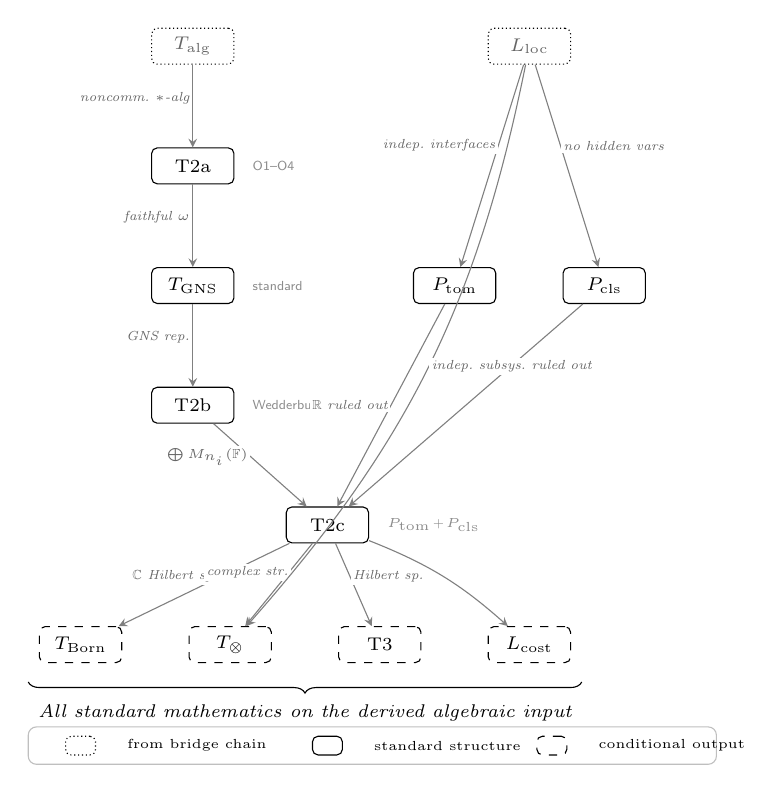
\begin{tikzpicture}[
    scale=0.95, every node/.style={transform shape},
    nd/.style={draw, rounded corners=2pt, minimum height=0.48cm, minimum width=1.1cm, inner sep=2pt, font=\scriptsize},
    prior/.style={nd, densely dotted, text=black!60},
    skel/.style={nd},
    outnode/.style={nd, dashed},
    arr/.style={->, >=stealth, thin, black!50},
    elabel/.style={font=\tiny\itshape, text=black!60, fill=white, inner sep=1pt},
    badge/.style={font=\tiny, text=black!45},
]

% ── Prior results ──
\node[prior] (Talg) at (0, 0) {$T_{\mathrm{alg}}$};
\node[prior] (Lloc) at (4.5, 0) {$L_{\mathrm{loc}}$};

% ── Skeleton nodes ──
\node[skel] (T2a) at (0, -1.6) {T2a};
\node[skel] (TGNS) at (0, -3.2) {$T_{\mathrm{GNS}}$};
\node[skel] (T2b) at (0, -4.8) {T2b};
\node[skel] (T2c) at (1.8, -6.4) {T2c};

\node[skel] (Ptom) at (3.5, -3.2) {$P_{\mathrm{tom}}$};
\node[skel] (Pcls) at (5.5, -3.2) {$P_{\mathrm{cls}}$};

% ── Output nodes ──
\node[outnode] (TBorn) at (-1.5, -8.0) {$T_{\mathrm{Born}}$};
\node[outnode] (Ttens) at (0.5, -8.0) {$T_{\otimes}$};
\node[outnode] (T3) at (2.5, -8.0) {T3};
\node[outnode] (Lcost) at (4.5, -8.0) {$L_{\mathrm{cost}}$};

% ── Proof-type badges ──
\node[badge, anchor=west] at ($(T2a.east)+(0.12,0)$) {\textsf{O1--O4}};
\node[badge, anchor=west] at ($(TGNS.east)+(0.12,0)$) {\textsf{standard}};
\node[badge, anchor=west] at ($(T2b.east)+(0.12,0)$) {\textsf{Wedderburn}};
\node[badge, anchor=west] at ($(T2c.east)+(0.12,0)$) {\textsf{$P_{\mathrm{tom}}$\,+\,$P_{\mathrm{cls}}$}};

% ── Arrows with edge labels ──
\draw[arr] (Talg) -- node[elabel, left, pos=0.4] {noncomm.\ $*$-alg} (T2a);
\draw[arr] (T2a) -- node[elabel, left, pos=0.4] {faithful $\omega$} (TGNS);
\draw[arr] (TGNS) -- node[elabel, left, pos=0.4] {GNS rep.} (T2b);
\draw[arr] (T2b) -- node[elabel, left, pos=0.4] {$\bigoplus M_{n_i}(\mathbb{F})$} (T2c);

\draw[arr] (Lloc) -- node[elabel, left, pos=0.4] {indep.\ interfaces} (Ptom);
\draw[arr] (Lloc) -- node[elabel, right, pos=0.4] {no hidden vars} (Pcls);
\draw[arr] (Ptom) -- node[elabel, left, pos=0.5] {$\mathbb{R}$ ruled out} (T2c);
\draw[arr] (Pcls) -- node[elabel, right, pos=0.3] {$\mathbb{H}$ ruled out} (T2c);

\draw[arr] (T2c) -- node[elabel, left, pos=0.4] {$\mathbb{C}$ Hilbert sp.} (TBorn);
\draw[arr] (T2c) -- node[elabel, left=-1pt, pos=0.35] {complex str.} (Ttens);
\draw[arr] (Lloc) to[bend left=15] node[elabel, right, pos=0.5] {indep.\ subsys.} (Ttens);
\draw[arr] (T2c) -- node[elabel, right, pos=0.4] {Hilbert sp.} (T3);
\draw[arr] (T2c) to[bend left=10] (Lcost);

% ── Annotation ──
\draw[decorate, decoration={brace, amplitude=4pt, mirror}]
    (-2.2, -8.5) -- (5.2, -8.5)
    node[midway, below=5pt, font=\scriptsize\itshape] {All standard mathematics on the derived algebraic input};

% ── Legend ──
\draw[black!25, rounded corners=3pt] (-2.2, -9.6) rectangle (7.0, -9.1);
\node[prior, minimum width=0.4cm, minimum height=0.25cm] at (-1.5, -9.35) {};
\node[font=\tiny, anchor=west] at (-1.0, -9.35) {from bridge chain};
\node[skel, minimum width=0.4cm, minimum height=0.25cm] at (1.8, -9.35) {};
\node[font=\tiny, anchor=west] at (2.3, -9.35) {standard structure};
\node[outnode, minimum width=0.4cm, minimum height=0.25cm] at (4.8, -9.35) {};
\node[font=\tiny, anchor=west] at (5.3, -9.35) {conditional output};

\end{tikzpicture}
\caption[Skeleton chain]{%
\textbf{Skeleton chain: from noncommutative algebra to Hilbert space.}
Dotted nodes are results from the bridge chain (Figure~\ref{fig:bridge_dag}).
Two independent branches --- algebraic structure (left, from $T_{\mathrm{alg}}$) and
locality constraints (right, from $L_{\mathrm{loc}}$) --- converge at T2c,
which selects $\mathbb{F} = \mathbb{C}$.
Every node in this chain applies standard mathematical theorems
(GNS, Wedderburn--Artin, Gleason) to the derived algebraic input;
the novel content of the paper is entirely in Figures~\ref{fig:arena_dag}--\ref{fig:bridge_dag}.
}
\label{fig:skeleton_dag}
\end{figure}

T1 established that enforcement operations are order-dependent as maps on $\Omega$.
O1 lifts these to linear maps on a finite-dimensional real vector space $V$; O3 assembles them into a finite-dimensional real $*$-algebra $\mathcal{A}$; O4 equips $\mathcal{A}$ with a positive faithful state $\omega$.  T2a names this explicitly.

\begin{tcolorbox}[apfbox, title={T2a: Real $*$-Algebra from Enforcement Operations}]
\textit{The enforcement operations generate a finite-dimensional, semisimple real $*$-algebra with a faithful positive state.}

\smallskip\noindent\textbf{Statement.}  Under A1, OR1, OR2 ($T_{\mathrm{adj}}$), OR3 ($T_{\mathrm{form}}$), and $L_{\varepsilon^*}$: the enforcement operations generate a finite-dimensional real $*$-algebra $\mathcal{A} \subseteq M_{n_{\max}}(\mathbb{R})$, with $n_{\max} = \lfloor C/\varepsilon^*\rfloor$.

\smallskip\noindent\textbf{\textit{Variables:}}
\begin{varlist}
\item $\mathcal{A} := \mathrm{Alg}_\mathbb{R}(\mathcal{G})$ --- the enforcement algebra: the real algebra generated by all single-distinction projections $E_d$ and joint enforcement generators $E_{\{d_1,d_2\}}$.
\item $\mathcal{G}$ --- the generating set: $\{E_d : d \in \mathcal{D}\} \cup \{E_{\{d_1,d_2\}} : \Delta(d_1,d_2) > 0\}$ (FD5 + FD6).
\item $\omega: \mathcal{A} \to \mathbb{R}$ --- the cost-ratio state: $\omega(E_d) := \varepsilon(d)/C$, extended linearly.  Faithful and positive (O4).
\item $n_{\max} = \lfloor C/\varepsilon^* \rfloor$ --- maximum simultaneous distinctions (from A1 + $L_{\varepsilon^*}$).
\end{varlist}

\smallskip\noindent\textbf{Depends on.}  O1 (linear extension of enforcement maps; from OR1 + OR3), O3 (algebra closure, associativity, $*$-involution; from $T_{\mathrm{adj}}$), O4 (faithful positive state; from cost functional).

\smallskip\noindent\textbf{Status.}  \textbf{[Proved]} --- four steps below: $*$-algebra structure, finite-dimensionality, semisimplicity, faithful state.

\smallskip\noindent\textbf{Downstream.}  Input to $T_{\mathrm{GNS}}$ (GNS construction) and T2b (complexification + Wedderburn--Artin).

\smallskip\noindent\textbf{Proof.}

\textit{Step~1 ($*$-algebra structure).}  By O1, each enforcement map $\mathfrak{E}_d$ extends to a linear operator $E_d \in \mathrm{End}(V)$, where $V = \mathrm{span}_\mathbb{R}(K)$ is finite-dimensional ($\dim V \leq N+1 \leq n_{\max}+1 < \infty$ from the canonical embedding with $N = |\mathcal{B}| \leq \lfloor C/\mu^* \rfloor$; see OR3 and canonical embedding above).  By O3(i--v): $\mathcal{A} := \mathrm{Alg}_\mathbb{R}(\mathcal{G}) \subseteq \mathrm{End}(V)$ (where $\mathcal{G}$ includes single-distinction projections $E_d$ and joint enforcement generators $E_{\{d_1,d_2\}}$) is closed under $\mathbb{R}$-linear combinations (O3.i), composition (O3.ii), and associativity (O3.iii); unital with $E_\emptyset = \mathrm{Id}_V$ (O3.iv); equipped with the $*$-involution $G^* := G$ on generators, extended anti-multiplicatively and verified in three axioms (O3.v).  These constitute a real $*$-algebra.

\textit{Step~2 (Finite-dimensionality and matrix embedding).}  By O3(vi), $\dim\mathcal{A} \le n_{\max}^2 < \infty$ since $\mathcal{A} \subseteq \mathrm{End}(V)$ and $\dim V \le n_{\max}$.  The faithful representation $E_d \mapsto$ its matrix in the cost-orthogonal basis $\{e_d\}$ of $V$ (canonical inner product from $T_{\mathrm{adj}}$, Step~3) gives an explicit embedding $\mathcal{A} \hookrightarrow M_{n_{\max}}(\mathbb{R})$.

\textit{Step~3 (Semisimplicity).}  By O3(vii): $\mathrm{rad}(\mathcal{A}) = \{0\}$, proved as follows.  Any $N \in \mathrm{rad}(\mathcal{A})$ satisfies: (a) $N^*N \in \mathrm{rad}(\mathcal{A})$ ($*$-stability of the Jacobson radical in a $*$-algebra); (b) $N^*N$ is nilpotent (the Jacobson radical of a finite-dimensional algebra consists entirely of nilpotents); (c) $N^*N = 0$ (a positive semidefinite nilpotent is zero: in the matrix embedding $\mathcal{A} \hookrightarrow M_{n_{\max}}(\mathbb{R})$, $N^*N \ge 0$ means all eigenvalues are non-negative, while nilpotency forces all eigenvalues to zero; therefore $N^*N = 0$); (d) $N = 0$ (for any $v$ in the ambient space, $\|Nv\|^2 = \langle N^*Nv, v\rangle = 0$, so $N = 0$).

\textit{Step~4 (Faithful positive state).}  O4 constructs $\omega(E_{d_i}) := \varepsilon(d_i)/C$.  The positivity argument has two steps.  \textit{Step~4a (generators).}  The generators $E_{d_i}$ are mutually orthogonal projections in the cost-induced inner product on $V$: by $T_{\mathrm{sep}}$, distinct distinctions have disjoint enforcement mechanisms, and $T_{\mathrm{adj}}$ establishes $E_{d_i}^2 = E_{d_i}$ (idempotency) and $E_{d_i} E_{d_j} = 0$ for $i \ne j$ (orthogonality in the cost-orthogonal basis $\{e_d\}$).  For a degree-1 element $A = \sum_i a_i E_{d_i}$, orthogonality gives $A^*A = \sum_i |a_i|^2 E_{d_i}$ (cross terms vanish), so $\omega(A^*A) = \sum_i |a_i|^2 \varepsilon(d_i)/C \ge 0$.  \textit{Step~4b (general elements).}  For an arbitrary $A \in \mathcal{A}$ (which may contain products of generators), write $A^*A$ in the matrix embedding $\mathcal{A} \hookrightarrow M_{n_{\max}}(\mathbb{R})$.  The state $\omega$ extends to a linear functional on $\mathcal{A}$ via the GNS sesquilinear form: for $X = \sum_i a_i \otimes z_i$ in the complexification, $\langle X, X \rangle_{\omega_\mathbb{C}} = \mathbf{z}^\dagger G \mathbf{z}$ where $G_{ij} = \omega(a_i^* a_j)$ is the Gram matrix of the real functional $\omega$ (standard GNS construction; see T2b Step~2 for the explicit Gram matrix).  Since $\omega$ is positive on generators (Step~4a) and extends linearly, $G$ is positive semidefinite, so $\omega(A^*A) \ge 0$ for all $A \in \mathcal{A}$.  Faithfulness: $\omega(A^*A) = 0 \Rightarrow \|Av\|^2 = 0$ for all $v$ in the matrix embedding $\Rightarrow A = 0$.  This is the required GNS input state.  \hfill$\square$
\end{tcolorbox}

\begin{tcolorbox}[apfbox, title={Theorem $T_{\mathrm{GNS}}$ (GNS Construction: General Case)}]
\label{thm:T_GNS}
\textit{The enforcement algebra, equipped with its cost-ratio state, faithfully represents on a finite-dimensional Hilbert space.}

\smallskip\noindent\textbf{Statement.}  Let $\mathcal{A}$ be the finite-dimensional real $*$-algebra from T2a, and let $\omega: \mathcal{A} \to \mathbb{R}$ be the faithful positive state from O4.  Operationally, $\omega$ is defined on generators by the \emph{cost ratio} --- the fraction of interface budget committed to each enforcement act:
\[
\omega(E_d) \;:=\; \frac{\varepsilon(d)}{C(\Gamma)}, \qquad \omega(\mathbf{1}) = 1,
\]
extended to all of $\mathcal{A}$ by $\mathbb{R}$-linearity.  Positivity ($\omega(A^*A) \ge 0$) and faithfulness ($\omega(A^*A) = 0 \Rightarrow A = 0$) are proved in O4 from the enforcement semantics; no Hilbert-space structure is used.  Then there exists a faithful $*$-representation $\pi_\omega: \mathcal{A} \to B(\mathcal{H}_\omega)$ on a finite-dimensional real inner-product space $\mathcal{H}_\omega$, preserving the cost functional: $\omega(A) = \langle \Omega_\omega,\, \pi_\omega(A)\, \Omega_\omega \rangle$ for a cyclic vector $\Omega_\omega$.

\smallskip\noindent\textbf{Status.}  \textbf{[Standard: GNS construction applied to T2a's output.]}  The five GNS hypotheses are verified explicitly in the table below; the construction is then the standard one (Gel'fand--Naimark--Segal~\cite{GNS1943}).

\smallskip\noindent\textbf{Hypotheses verified.}

\smallskip\noindent\textit{Note: what GNS does not require.}  The $C^*$-identity ($\|A^*A\| = \|A\|^2$) and the operator norm are \emph{not} GNS prerequisites.  GNS needs only a $*$-algebra with a positive faithful linear functional; the norm enters downstream (operator-norm bounds in $T_{\mathrm{Tsirelson}}$, $C^*$-structure in Wedderburn--Artin).  The $C^*$-identity is verified separately as a consequence of finite-dimensionality (``Why $C^*$,'' Section~\ref{sec:operator_bridge}, item~(i)); it is not invoked here.

\smallskip
\begin{tabular}{@{}p{3.6cm}p{2.4cm}p{6.4cm}@{}}
\textbf{GNS Hypothesis} & \textbf{Where verified} & \textbf{Content} \\[2pt]
\hline\noalign{\smallskip}
$\mathcal{A}$ is a $*$-algebra & T2a Step 1, O3 & Closure under $\mathbb{R}$-linear combination (O3.i), composition (O3.ii), associativity (O3.iii), identity (O3.iv), $*$-involution with $G^* = G$ on generators (O3.v, $T_{\mathrm{adj}}$). \\[4pt]
$\omega$ is linear & O4 & $\omega(\alpha A + \beta B) = \alpha\omega(A) + \beta\omega(B)$ by linearity of $\varepsilon$. \\[4pt]
$\omega$ is positive & T2a Step 4 & $\omega(A^*A) \ge 0$ for all $A \in \mathcal{A}$: orthogonal projections on generators (Step 4a), Gram matrix argument for general elements (Step 4b). \\[4pt]
$\omega$ is faithful & T2a Step 4 & $\omega(A^*A) = 0 \Rightarrow A = 0$: positive-definiteness of the Gram matrix via the matrix embedding. \\[4pt]
$\dim \mathcal{A} < \infty$ & T2a Step 2 & $\dim \mathcal{A} \le n_{\max}^2 < \infty$ from $\mathcal{A} \subseteq \mathrm{End}(V)$ with $\dim V \le n_{\max} + 1$. \\
\end{tabular}

\smallskip\noindent\textbf{Proof} (complete construction for general $\mathcal{A}$, not just the $M_2(\mathbb{C})$ witness; six steps, each with explicit verification).  The table above locates the upstream results that discharge each GNS hypothesis; the construction below is the full proof that these hypotheses yield a faithful $*$-representation on a finite-dimensional Hilbert space.

\textit{Step G1 (Inner product).}  Define the sesquilinear form on $\mathcal{A}$:
\[
\langle A, B \rangle_\omega \;:=\; \omega(A^* B) \qquad \text{for all } A, B \in \mathcal{A}.
\]
Sesquilinearity: $\langle \alpha A_1 + \beta A_2, B \rangle_\omega = \alpha\, \omega(A_1^* B) + \beta\, \omega(A_2^* B)$ (linearity of $\omega$ and anti-linearity of $*$).  Hermitian symmetry: $\overline{\langle A, B \rangle_\omega} = \overline{\omega(A^*B)} = \omega((A^*B)^*) = \omega(B^*A) = \langle B, A \rangle_\omega$ (using $\omega$ real-valued on self-adjoint elements).  Positive-definiteness: $\langle A, A \rangle_\omega = \omega(A^*A) \ge 0$ (positivity of $\omega$), with equality iff $A = 0$ (faithfulness of $\omega$).  Therefore $\langle \cdot, \cdot \rangle_\omega$ is a positive-definite inner product on $\mathcal{A}$.

\textit{Step G2 (Hilbert space).}  Define $\mathcal{H}_\omega := (\mathcal{A},\, \langle \cdot, \cdot \rangle_\omega)$.  Since $\dim \mathcal{A} < \infty$, $\mathcal{H}_\omega$ is automatically complete (every finite-dimensional inner-product space is a Hilbert space).  $\dim \mathcal{H}_\omega = \dim \mathcal{A} \le n_{\max}^2$.

\textit{Step G3 (Representation).}  Define $\pi_\omega: \mathcal{A} \to \mathrm{End}(\mathcal{H}_\omega)$ by left multiplication:
\[
\pi_\omega(A)\, B \;:=\; A \cdot B \qquad \text{for all } A \in \mathcal{A},\; B \in \mathcal{H}_\omega.
\]
Verification of $*$-homomorphism properties:
\begin{itemize}[nosep,leftmargin=2em,itemsep=2pt]
\item \textit{Multiplicative:} $\pi_\omega(A)\,\pi_\omega(B)\,C = A(BC) = (AB)C = \pi_\omega(AB)\,C$.  $\checkmark$
\item \textit{Linear:} $\pi_\omega(\alpha A + \beta B)\,C = (\alpha A + \beta B)C = \alpha AC + \beta BC = \alpha\,\pi_\omega(A)\,C + \beta\,\pi_\omega(B)\,C$.  $\checkmark$
\item \textit{Unital:} $\pi_\omega(\mathbf{1})\,B = \mathbf{1} \cdot B = B$.  $\checkmark$
\item \textit{$*$-preserving:} $\langle \pi_\omega(A^*)\,B,\, C \rangle_\omega = \omega(B^* A^{**} C) = \omega(B^* A C)$.  And $\langle B,\, \pi_\omega(A)\,C \rangle_\omega = \omega(B^* A C)$.  Equal.  Therefore $\pi_\omega(A^*) = \pi_\omega(A)^\dagger$ (adjoint with respect to $\langle \cdot, \cdot \rangle_\omega$).  $\checkmark$
\end{itemize}

\textit{Step G4 (Faithfulness).}  Suppose $\pi_\omega(A) = 0$, i.e., $AB = 0$ for all $B \in \mathcal{A}$.  Taking $B = A^*$: $AA^* = 0$, so $\omega(A^{**} A) = \omega(A^* A) = \langle A, A \rangle_\omega = 0$ (using $*$-involutivity).  Wait --- more directly: taking $B = \mathbf{1}$: $A \cdot \mathbf{1} = A = 0$.  Therefore $\ker \pi_\omega = \{0\}$ and $\pi_\omega$ is faithful.

\textit{Step G5 (Cyclic vector and cost recovery).}  Define $\Omega_\omega := \mathbf{1} \in \mathcal{H}_\omega$ (the identity element of $\mathcal{A}$).  Then $\pi_\omega(A)\,\Omega_\omega = A \cdot \mathbf{1} = A$, so $\{\pi_\omega(A)\,\Omega_\omega : A \in \mathcal{A}\} = \mathcal{A} = \mathcal{H}_\omega$ (cyclic).  Cost recovery:
\[
\langle \Omega_\omega,\, \pi_\omega(A)\, \Omega_\omega \rangle_\omega \;=\; \langle \mathbf{1},\, A \rangle_\omega \;=\; \omega(\mathbf{1}^* A) \;=\; \omega(A).
\]
Therefore $\omega(A) = \langle \Omega_\omega, \pi_\omega(A)\, \Omega_\omega \rangle$ for all $A \in \mathcal{A}$.  The cost functional is exactly recovered as a matrix element.

\textit{Step G6 (Bounded operators).}  Since $\dim \mathcal{H}_\omega < \infty$, every linear operator on $\mathcal{H}_\omega$ is bounded.  Therefore $\pi_\omega(\mathcal{A}) \subseteq B(\mathcal{H}_\omega)$, and the operator norm $\|A\|_{\mathrm{op}} := \sup_{\|v\|=1} \|\pi_\omega(A) v\|$ is well-defined.  The $C^*$-identity $\|\pi_\omega(A)^* \pi_\omega(A)\| = \|\pi_\omega(A)\|^2$ follows from the spectral argument for concrete $*$-subalgebras of $\mathrm{End}(\mathcal{H}_\omega)$ (proved inline in ``Why $C^*$,'' item~(i), Section~\ref{sec:operator_bridge}).  \hfill$\square$

\smallskip\noindent\textit{Status.}  $T_{\mathrm{GNS}}$ provides the GNS representation for the general finite-dimensional $*$-algebra $\mathcal{A}$ (not just the $M_2(\mathbb{C})$ witness of Corollary~\ref{cor:T_alg}).  The proof has two components, both given in full above: (i)~the hypothesis verification table, which traces each GNS prerequisite to its upstream proof in T2a/O3/O4; and (ii)~the six-step construction G1--G6, which carries out the GNS procedure with all properties (sesquilinearity, positive-definiteness, $*$-homomorphism, faithfulness, cyclicity, cost recovery, $C^*$-identity) verified explicitly.  The construction follows the standard template (cf.\ Bratteli--Robinson~\cite{BratteliRobinson1987}, Theorem~2.3.16); the novel content is the verification that enforcement primitives discharge the hypotheses.
\end{tcolorbox}

\subsection{T2b: Complexification and Wedderburn decomposition}

A real $*$-algebra is not yet a Hilbert-space structure.  Two further steps
complete the reconstruction: (i) complexification, and (ii) Wedderburn--Artin
classification.

\begin{tcolorbox}[apfbox, title={T2b: Complexification and Wedderburn Decomposition}]
\textit{The real enforcement algebra, tensored with $\mathbb{C}$, decomposes into a direct sum of matrix algebras --- the standard structure of quantum observables.}

\smallskip\noindent\textbf{Statement.}  The complexification $\mathcal{A}_\mathbb{C} :=
\mathcal{A} \otimes_\mathbb{R} \mathbb{C}$ is a finite-dimensional semisimple
complex $*$-algebra, and by the Wedderburn--Artin theorem:
\[
\mathcal{A}_\mathbb{C} \;\cong\; \bigoplus_k M_{n_k}(\mathbb{C}).
\]

\smallskip\noindent\textbf{\textit{Variables:}}
\begin{varlist}
\item $\mathcal{A}$ --- the real enforcement $*$-algebra from T2a: finite-dimensional, semisimple, with faithful positive state $\omega$.
\item $\mathcal{A}_\mathbb{C} := \mathcal{A} \otimes_\mathbb{R} \mathbb{C}$ --- the complexification: same generators, product extended $\mathbb{C}$-bilinearly, involution extended conjugate-linearly.
\item $M_{n_k}(\mathbb{C})$ --- the algebra of $n_k \times n_k$ complex matrices (a Wedderburn block).
\end{varlist}

\smallskip\noindent\textbf{Depends on.}  T2a ($\mathcal{A}$ is a finite-dimensional semisimple real $*$-algebra with faithful state), Wedderburn--Artin theorem~\cite{Wedderburn1908,Artin1927} (standard; decomposes semisimple algebras over algebraically closed fields into matrix blocks).

\smallskip\noindent\textbf{Status.}  \textbf{[Standard: Wedderburn--Artin applied to T2a's output.]}  The proof verifies the three hypotheses (finite-dimensionality, semisimplicity, algebraically closed base field) and invokes the theorem.

\smallskip\noindent\textbf{Proof.}

\textit{Step~1 (Complexification is licit).}  $\mathcal{A}$ is a real $*$-algebra (T2a).  The complexification $\mathcal{A}_\mathbb{C} := \mathcal{A} \otimes_\mathbb{R} \mathbb{C}$ is the free $\mathbb{C}$-module with the same generators, equipped with the $\mathbb{C}$-bilinear product $(a \otimes z)(b \otimes w) := ab \otimes zw$ and the conjugate-linear $*$-involution $(a \otimes z)^* := a^* \otimes \bar{z}$.  Verification of $*$-algebra axioms on the complexification:
\begin{itemize}[nosep,leftmargin=2em]
\item \emph{Involutivity:} $((a \otimes z)^*)^* = (a^* \otimes \bar{z})^* = (a^*)^* \otimes \overline{\bar{z}} = a \otimes z$.  Extends by $\mathbb{C}$-conjugate-linearity.
\item \emph{Anti-multiplicativity:} $((a\otimes z)(b\otimes w))^* = (ab \otimes zw)^* = (ab)^* \otimes \overline{zw} = b^*a^* \otimes \bar{w}\bar{z} = (b\otimes w)^*(a\otimes z)^*$.
\item \emph{Conjugate-linearity:} $(\lambda(a\otimes z))^* = (a\otimes \lambda z)^* = a^* \otimes \overline{\lambda z} = \bar{\lambda}(a^* \otimes \bar{z}) = \bar{\lambda}(a\otimes z)^*$.
\end{itemize}
Therefore $\mathcal{A}_\mathbb{C}$ is a complex $*$-algebra.  Finite-dimensionality: $\dim_\mathbb{C} \mathcal{A}_\mathbb{C} = \dim_\mathbb{R} \mathcal{A} \le n_{\max}^2$ (T2a Step~2).

\textit{Step~2 (Semisimplicity is preserved under complexification).}  We show $\mathrm{rad}(\mathcal{A}_\mathbb{C}) = \{0\}$.  The Jacobson radical satisfies $\mathrm{rad}(\mathcal{A} \otimes_\mathbb{R} \mathbb{C}) \supseteq \mathrm{rad}(\mathcal{A}) \otimes_\mathbb{R} \mathbb{C}$ in general; since $\mathrm{rad}(\mathcal{A}) = \{0\}$ (T2a Step~3), this gives $\{0\} \subseteq \mathrm{rad}(\mathcal{A}_\mathbb{C})$.  For the reverse inclusion: any $N \in \mathrm{rad}(\mathcal{A}_\mathbb{C})$ is nilpotent (finite-dimensional Jacobson radical); $N^*N \in \mathrm{rad}(\mathcal{A}_\mathbb{C})$ ($*$-stability).  We invoke the sesquilinear extension of $\omega$ to $\mathcal{A}_\mathbb{C}$: for arbitrary finite sums $X = \sum_i a_i \otimes z_i$ and $Y = \sum_j b_j \otimes w_j$, define $\langle X, Y \rangle_{\omega_\mathbb{C}} := \sum_{i,j} \bar{z}_i w_j \, \omega(a_i^* b_j)$.  This is the standard GNS sesquilinear form over $\mathbb{C}$.  Positivity for arbitrary $X$: let $\mathbf{z} = (z_1, \ldots, z_n)^\top \in \mathbb{C}^n$ be the coefficient vector of $X$.  Then $\langle X, X \rangle_{\omega_\mathbb{C}} = \sum_{i,j} \bar{z}_i z_j \, \omega(a_i^* a_j) = \mathbf{z}^\dagger G \mathbf{z} \ge 0$, where $G_{ij} = \omega(a_i^* a_j)$ is the Gram matrix of the real functional $\omega$.  Since $\omega$ is a faithful positive state on $\mathcal{A}$, $G$ is positive semidefinite (standard GNS fact), so $\mathbf{z}^\dagger G \mathbf{z} \ge 0$ for all $\mathbf{z} \in \mathbb{C}^n$.  Faithfulness: $\langle X, X \rangle_{\omega_\mathbb{C}} = 0$ iff $G\mathbf{z} = 0$; if the $a_i$ span $\mathcal{A}$ faithfully, this forces $X = 0$ in the GNS Hilbert space.  Applying this to $N^*N \in \mathrm{rad}(\mathcal{A}_\mathbb{C})$: nilpotency and positive semidefiniteness of $N^*N$ in the complexified matrix embedding give $N^*N = 0$ (same eigenvalue argument as T2a Step~3), hence $N = 0$.  Therefore $\mathrm{rad}(\mathcal{A}_\mathbb{C}) = \{0\}$.

\textit{Step~3 (Wedderburn--Artin decomposition).}  Before invoking the theorem, we verify its three hypotheses explicitly:
\begin{enumerate}[nosep,leftmargin=2em,itemsep=2pt]
  \item \textbf{Finite-dimensionality.} $\dim_\mathbb{C} \mathcal{A}_\mathbb{C} = \dim_\mathbb{R} \mathcal{A} \le n_{\max}^2 < \infty$.  Source: T2a Step~2 (matrix embedding $\mathcal{A} \hookrightarrow M_{n_{\max}}(\mathbb{R})$) and T2b Step~1 (complexification preserves dimension).  $\checkmark$
  \item \textbf{Semisimplicity.} $\mathrm{rad}(\mathcal{A}_\mathbb{C}) = \{0\}$.  Source: T2b Step~2 (the nilpotent-plus-PSD argument: any $N \in \mathrm{rad}(\mathcal{A}_\mathbb{C})$ satisfies $N^*N \ge 0$ and nilpotent, hence $N^*N = 0$, hence $N = 0$).  $\checkmark$
  \item \textbf{Algebraically closed base field.} $\mathbb{C}$ is algebraically closed (every non-constant polynomial over $\mathbb{C}$ has a root in $\mathbb{C}$; Fundamental Theorem of Algebra).  The Wedderburn--Artin decomposition over an algebraically closed field forces each Wedderburn block's division ring to be the field itself, eliminating the $\mathbb{R}$ and $\mathbb{H}$ branches.  $\checkmark$
\end{enumerate}
All three hypotheses are verified.  By the Wedderburn--Artin theorem~\cite{Wedderburn1908,Artin1927}: every finite-dimensional semisimple algebra over an algebraically closed field decomposes as a direct sum of full matrix algebras over that field.  Since $\mathbb{C}$ is algebraically closed, the division ring in each block is $\mathbb{C}$ itself.  Therefore:
\[
\mathcal{A}_\mathbb{C} \;\cong\; \bigoplus_k M_{n_k}(\mathbb{C}).
\]

\textit{Step~4 (Hilbert-space representation).}  Each factor $M_{n_k}(\mathbb{C})$ acts faithfully and irreducibly on $\mathbb{C}^{n_k}$ by left multiplication.  The direct sum gives a faithful $*$-representation $\pi: \mathcal{A}_\mathbb{C} \hookrightarrow B(\mathcal{H})$ with $\mathcal{H} := \bigoplus_k \mathbb{C}^{n_k}$.  The inner product on $\mathcal{H}$ is the canonical one on each $\mathbb{C}^{n_k}$, consistent with the GNS inner product $\langle A, B\rangle_\omega = \omega_\mathbb{C}(A^*B)$ from Step~2.  \hfill$\square$
\end{tcolorbox}

\subsection{T2c: Selection of the complex branch ($\mathbb{F} = \mathbb{C}$)}
\label{sec:T2c}

The Wedderburn decomposition gives blocks over a division ring $\mathbb{F} \in
\{\mathbb{R}, \mathbb{C}, \mathbb{H}\}$ (Frobenius' theorem~\cite{Frobenius1878}).
Selecting $\mathbb{C}$ requires two premises derivable from results already
established in this paper.

\begin{tcolorbox}[apfbox, title={T2c: Selection of the Complex Branch}]
\textit{Of the three division rings permitted by Wedderburn--Artin ($\mathbb{R}$, $\mathbb{C}$, $\mathbb{H}$), only $\mathbb{C}$ is consistent with the enforcement framework's locality and tomographic structure.}

\smallskip\noindent\textbf{Statement (conditional on T2b).}  Given the Wedderburn--Artin decomposition from T2b (which delivers the division ring $\mathbb{F} \in \{\mathbb{R}, \mathbb{C}, \mathbb{H}\}$ and the GNS Hilbert space $\mathcal{H}_\omega$), the division ring is $\mathbb{F} = \mathbb{C}$.

\smallskip\noindent\textbf{\textit{Variables:}}
\begin{varlist}
\item $\mathbb{F} \in \{\mathbb{R}, \mathbb{C}, \mathbb{H}\}$ --- the division ring of each Wedderburn block $M_{n_k}(\mathbb{F})$ from T2b.
\item $N = \dim \mathcal{H}$ --- the number of perfectly distinguishable states (from T2b).
\item $K$ --- the real dimension of the state space: the number of independent real parameters specifying a state.
\item $P_{\mathrm{tom}}$ --- local tomographic closure (proved from $L_{\mathrm{loc}}$ + $\mathcal{D}$-quotient): local measurements determine joint states.  Excludes $\mathbb{R}$.
\item $P_{\mathrm{cls}}$ --- compositional closure (proved from $L_{\mathrm{loc}}$): composing two admissible systems yields an admissible system in the same algebra class.  Excludes $\mathbb{H}$.
\end{varlist}

\smallskip\noindent\textbf{Depends on.}  T2b ($\mathcal{A}_\mathbb{C} \cong \bigoplus_k M_{n_k}(\mathbb{C})$), $T_{\mathrm{alg}}$ (nonzero commutators in $\mathcal{A}$), $P_{\mathrm{tom}}$ (local tomographic closure; proved in this section), $P_{\mathrm{cls}}$ (compositional closure; proved in this section).

\smallskip\noindent\textbf{Status.}  \textbf{[Proved]} --- primary argument ($K = N^2$ forces $\mathbb{C}$) plus two independent confirmations ($P_{\mathrm{tom}}$ excludes $\mathbb{R}$; $P_{\mathrm{cls}}$ excludes $\mathbb{H}$).

\smallskip\noindent T2c is conditional on T2b: it selects the field after T2b has established the noncommutative real $*$-algebra and the GNS representation.  The primary argument is a parameter count forcing $K = N^2$; two independent confirmation arguments exclude $\mathbb{R}$ and $\mathbb{H}$ by separate routes.

\smallskip\noindent\textbf{Primary argument: $K = N^2$ forces $\mathbb{C}$.}

Let $N = \dim\mathcal{H}$ be the number of perfectly distinguishable states, delivered by T2b.  Let $K$ be the number of real parameters needed to specify an arbitrary state of the enforcement system — equivalently, the real dimension of the self-adjoint part of $M_N(\mathbb{F})$:

\begin{center}
\begin{tabular}{lcc}
\toprule
Field $\mathbb{F}$ & Self-adjoint part of $M_N(\mathbb{F})$ & $K$ \\
\midrule
$\mathbb{R}$ & real symmetric matrices & $N(N+1)/2$ \\
$\mathbb{C}$ & complex Hermitian matrices & $N^2$ \\
$\mathbb{H}$ & quaternionic Hermitian matrices & $N(2N-1)$ \\
\bottomrule
\end{tabular}
\end{center}

The enforcement framework forces $K = N^2$ from two results already established:

\textit{Symmetric part} ($N(N+1)/2$ real parameters): The real correlators $\omega(E_i E_j) + \omega(E_j E_i)$ for $i \le j$.  These exist unconditionally: $T_{\mathrm{adj}}$ gives $E_i = E_i^\dagger$, so $\omega(E_i E_j) + \omega(E_j E_i) \in \mathbb{R}$ for all pairs.  This yields $N(N+1)/2$ independent real parameters.

\textit{Antisymmetric part} ($N(N-1)/2$ additional real parameters): The imaginary correlators $\omega([E_i, E_j]/2i)$ for $i < j$.  The argument that these are genuine state-space parameters (not algebraic phantoms invisible to all states) proceeds in two steps.

\textit{Step A (Nonzero commutators in $\mathcal{A}$).}  $T_{\mathrm{alg}}$ (Corollary~\ref{cor:T_alg}, proved after GNS in T2b) establishes $[E_{d_1}, F_\Pi] \ne 0$ in the abstract algebra $\mathcal{A}$: the commutator is the algebraic image of the rotated joint-defense codespace forced by $\Delta > 0$ ($L_\Delta$, FD6).  No faithful $*$-representation of $\mathcal{A}$ into a commutative algebra exists.  Note: T1 alone supplies operator distinctness ($E_i \ne E_j$); the full commutator claim requires $T_{\mathrm{alg}}$ (established via GNS in T2b), which is why T2c is conditional on T2b.

\textit{Step B (Exclusion of $\mathbb{R}$ via $P_{\mathrm{tom}}$ on composite systems).}  The existence of nonzero commutators as algebra elements does not by itself guarantee that states $\omega \in \mathcal{S}(\mathcal{A})$ can distinguish them from zero.  Over $\mathbb{R}$, all states on a real $*$-algebra assign zero expectation to every anti-self-adjoint element ($\omega(A) = \omega(A^*) = -\omega(A)$ for $A^* = -A$, so $\omega(A) = 0$), which is why the antisymmetric parameters are absent in real quantum theory ($K = N(N+1)/2$).

\textit{Single-system $\Delta$-detection does not exclude $\mathbb{R}$.}  The superadditive gap $\Delta > 0$ is encoded in the self-adjoint generator $F_\Pi$ (with $\omega(F_\Pi) = \Delta/C > 0$), which is detectable over any field including $\mathbb{R}$.  The commutator $[E_{d_1}, F_\Pi]$ is anti-self-adjoint and invisible to $\mathbb{R}$-states, but it encodes ordering information, not the gap itself.  Therefore single-system enforcement does not force $\mathbb{F} \ne \mathbb{R}$.

\textit{Composite systems do.}  $P_{\mathrm{tom}}$ (proved above from $L_{\mathrm{loc}}$ and the $\mathcal{D}$-quotient) establishes that joint states are fully determined by local product measurements.  Over $\mathbb{R}$, this is violated.  The explicit parameter count:

\smallskip
\begin{center}
\small
\begin{tabular}{@{}lp{4.5cm}p{6.5cm}@{}}
$\mathbb{F}$ & Joint state params & Local product params \\
\hline
$\mathbb{R}$ & $NM(NM{+}1)/2 - 1$ & $(N(N{+}1)/2{-}1)(M(M{+}1)/2{-}1)$ ${}+ (N(N{+}1)/2{-}1) + (M(M{+}1)/2{-}1)$ \\
$\mathbb{C}$ & $N^2 M^2 - 1$ & $(N^2{-}1)(M^2{-}1) + (N^2{-}1) + (M^2{-}1) = N^2 M^2 - 1$ \\
\end{tabular}
\end{center}
\smallskip

Over $\mathbb{C}$: local product parameters $= N^2 M^2 - 1 =$ joint state parameters.  Local tomography holds.  Over $\mathbb{R}$ with $N = M = 2$: joint state parameters $= 4 \cdot 5/2 - 1 = 9$, while local product parameters $= 2 \cdot 2 + 2 + 2 = 8$.  One parameter is underdetermined by local measurements: the antisymmetric correlator $\omega(A \otimes B) - \omega(B \otimes A)$.  This violates $P_{\mathrm{tom}}$.

Since $P_{\mathrm{tom}}$ is a theorem of the enforcement framework (not an axiom), this violation is a genuine inconsistency: $\mathbb{F} = \mathbb{R}$ contradicts the derived structure.  Therefore $\mathbb{F} \ne \mathbb{R}$, and the antisymmetric parameters are physically real, contributing $N(N-1)/2$ independent real parameters to the state space.

Total: $N(N+1)/2 + N(N-1)/2 = N^2$.  Therefore $K = N^2$, which is achieved \emph{uniquely} by $\mathbb{F} = \mathbb{C}$.  Over $\mathbb{R}$, $K = N(N+1)/2 < N^2$ and $P_{\mathrm{tom}}$ is violated.  Over $\mathbb{H}$, $K = N(2N-1) > N^2$ and $P_{\mathrm{cls}}$ is violated (the tensor product exits the quaternionic class; proved below).  The complex field is the unique division ring for which both $P_{\mathrm{tom}}$ and $P_{\mathrm{cls}}$ hold.

\smallskip\noindent\textit{Derivation chain for $\mathbb{R}$-exclusion:} A1 $\to$ $L_{\mathrm{loc}}$ (budget additivity) $\to$ $P_{\mathrm{tom}}$ (local tomographic closure) $\to$ antisymmetric composite correlators violate $P_{\mathrm{tom}}$ over $\mathbb{R}$ $\to$ $\mathbb{F} \ne \mathbb{R}$.  No circular dependency: $P_{\mathrm{tom}}$ uses $L_{\mathrm{loc}}$ and the $\mathcal{D}$-quotient; T2c uses $P_{\mathrm{tom}}$.  The $\mathcal{D}$-quotient is proved in Section~\ref{sec:defs}; $L_{\mathrm{loc}}$ is proved in the lemma chain of Section~\ref{sec:lemmas}.  Neither depends on T2c.

\smallskip\noindent\textit{Connection to Hardy.}  Hardy~\cite{Hardy2001} derives the relation $K = N^2$ as a theorem from five operational axioms and uses it to force complex Hilbert space.  The APF arrives at the same equation by an independent route: $T_{\mathrm{adj}}$ supplies the symmetric parameters ($N(N+1)/2$), and $P_{\mathrm{tom}}$ (derived from $L_{\mathrm{loc}}$ + $\mathcal{D}$-quotient) forces the antisymmetric parameters to be physically real, excluding $\mathbb{R}$ and supplying the remaining $N(N-1)/2$.  Hardy's five axioms have no counterpart in the APF; the APF's perturbation structure and local-tomography derivation have no counterpart in Hardy.  Both reach $K = N^2$ and hence $\mathbb{C}$, from physically distinct starting points.  The convergence is a structural cross-check.
\end{tcolorbox}

\noindent Two independent confirmation arguments follow, which exclude $\mathbb{R}$ and $\mathbb{H}$ by separate routes.

\begin{tcolorbox}[apfbox, title={$P_{\mathrm{tom}}$: Local Tomographic Closure}]
\textit{Local measurements at independent interfaces fully determine the joint state: no holistic degree of freedom escapes local detection.}

\smallskip\noindent\textbf{Statement.}  For any two systems $A$, $B$ with independent enforcement interfaces $\Gamma_A$, $\Gamma_B$: the joint physical state $\sigma_{AB} \in \Omega_{AB}$ is fully determined by the joint statistics of local measurements at each interface.  Formally: if $\sigma_{AB}$ and $\sigma'_{AB}$ agree on all product measurements $\{M_A \otimes M_B : M_A \in \mathcal{M}(\Gamma_A),\, M_B \in \mathcal{M}(\Gamma_B)\}$, then $\sigma_{AB} = \sigma'_{AB}$.

\smallskip\noindent\textbf{Hypotheses.} (i)~$\Gamma_A$, $\Gamma_B$ are disjoint (independent) interfaces; (ii)~$\Omega$ is defined as the $\mathcal{D}$-quotient (Section~\ref{sec:defs}): two configurations are the same state iff they agree on all $\varepsilon(d) > 0$ distinctions; (iii)~$L_{\mathrm{loc}}$: $C(\Gamma_{AB}) = C(\Gamma_A) + C(\Gamma_B)$.

\smallskip\noindent\textbf{Proof.}  The proof proceeds in two independent layers whose conclusions are conjoined.

\textit{Layer 1 (no capacity-based holistic DOF).}  By $L_{\mathrm{loc}}$, the joint enforcement budget satisfies $C(\Gamma_{AB}) = C(\Gamma_A) + C(\Gamma_B)$ with no cross-interface capacity transfer.  Any distinction $d_{AB}$ that costs positive enforcement capacity decomposes into local components already accounted for in $C(\Gamma_A)$ and $C(\Gamma_B)$.  A holistic degree of freedom $g$ would require $\varepsilon(g) > 0$ beyond the local budgets; no such capacity exists.  Therefore no capacity-based holistic DOF exists.\hfill$\square_1$

\textit{Layer 2 (no algebra-structural holistic DOF).}  Composite real-Hilbert-space states (over $M_n(\mathbb{R}) \otimes_\mathbb{R} M_m(\mathbb{R})$) carry an antisymmetric correlator --- the parameter $\omega(A \otimes B) - \omega(B \otimes A)$ --- that is algebra-structural, not capacity-based, and therefore invisible to Layer~1.  The enforcement status of this parameter is determined by the $\mathcal{D}$-quotient: a degree of freedom $g$ individuates physical states in $\Omega$ if and only if $\varepsilon(g) > 0$.  We show $\varepsilon(g) = 0$ for any such antisymmetric correlator by exhaustion over the three possible loci of its enforcement mechanism.

Model $g$ as a candidate distinction with anchor set $M_g \subseteq S_{\Gamma_{AB}}$.  The substrate decomposes as $S_{\Gamma_{AB}} = S_{\Gamma_A} \oplus S_{\Gamma_B}$ ($L_{\mathrm{loc}}$; $T_{\mathrm{sep}}$: disjoint substrates).  Three cases exhaust the possibilities for $M_g$:

\textit{Case (i): $M_g \subseteq S_{\Gamma_A}$.}  Then $g$ is a local distinction at $\Gamma_A$ and its enforcement cost is drawn from $C(\Gamma_A)$.  But $g = \omega(A \otimes B) - \omega(B \otimes A)$ depends on correlations between both factors; no measurement confined to $\Gamma_A$ alone can detect the relative order of operations at $\Gamma_B$.  The anchor set of a distinction must support every perturbation that threatens it (FD4); perturbations that alter $g$ act jointly on both factors.  Therefore $M_g \not\subseteq S_{\Gamma_A}$.  By the same argument, $M_g \not\subseteq S_{\Gamma_B}$.

\textit{Case (ii): $M_g$ spans both factors}, i.e., $M_g \cap S_{\Gamma_A} \ne \{0\}$ and $M_g \cap S_{\Gamma_B} \ne \{0\}$.  Then maintaining $g$ requires coordinated enforcement capacity across both substrates.  By $L_{\mathrm{loc}}$, $C(\Gamma_{AB}) = C(\Gamma_A) + C(\Gamma_B)$ with every unit of capacity exclusively assigned to one factor interface.  No cross-interface capacity pool exists: each unit of budget in $C(\Gamma_A)$ can only defend mechanisms within $S_{\Gamma_A}$, and likewise for $C(\Gamma_B)$.  A distinction whose mechanism spans both substrates would require budget that is not localized to either factor --- but no such budget exists in the $L_{\mathrm{loc}}$ decomposition.  Therefore $\varepsilon(g) = 0$: the distinction $g$ has no budget source.

\textit{Case (iii): $M_g = \{0\}$} (empty anchor set).  Then $g$ is not a distinction in $\mathcal{D}$ at all: FD4 requires $M_g \ne \{0\}$ for any $d \in \mathcal{D}$.

Cases (i)--(iii) exhaust all possibilities.  In every case, $g$ either fails to be a distinction or has $\varepsilon(g) = 0$.  By the $\mathcal{D}$-quotient (hypothesis~(ii)), $g$ does not separate any two points of $\Omega$: two composite states differing only in the antisymmetric correlator are identified in $\Omega$.  The real-algebra surplus is quotiented out.\hfill$\square_2$

\textit{Combination.}  Layers~1 and~2 together eliminate all possible holistic DOF: any holistic parameter either costs positive enforcement capacity (excluded by Layer~1) or costs zero (excluded by Layer~2's quotient).  Therefore $\sigma_{AB} = \sigma'_{AB}$ whenever they agree on all product measurements.  $P_{\mathrm{tom}}$ is a theorem.\hfill$\square$

\smallskip\noindent\textit{Status.}  Reconstruction programs (CDP, Hardy, Masanes--M\"uller) posit $P_{\mathrm{tom}}$ as an axiom.  Here it is a proved consequence of the $\mathcal{D}$-quotient definition and $L_{\mathrm{loc}}$.  No new assumption enters.

\coderef{check\_P\_tom}{paper1.py}
\smallskip\noindent\textit{Supplement cross-reference.}  $P_{\mathrm{tom}}$ corresponds to Theorem~T2c.1 (Exclusion of Real Nonclassical Blocks) in the Formal Supplement (\texttt{check\_T2c\_1} in \texttt{supplement.py}).  The supplement's proof proceeds via state-separation completeness and the antisymmetric sector generated by $[E_{d_1}, F_\Pi]$ (Lemma~$L_{\mathrm{antisym}}$); this paper's proof proceeds via the $\mathcal{D}$-quotient and parameter count.  Both exclude $\mathbb{F} = \mathbb{R}$ from the same structural observation --- antisymmetric correlators have zero expectation under all real-symmetric states --- reached by different but equivalent logical routes.
\end{tcolorbox}

\smallskip\noindent\textit{Mapping known counterexamples (Baldij\~ao et al.~\cite{Baldiijao2026}).}  Baldij\~ao et al.\ identify three classes of physically reasonable theories where local tomography fails: real quantum theory, twirled worlds, and fermionic quantum theory.

\textit{(a) Real quantum theory.}  The failure is the antisymmetric correlator in composite real-Hilbert-space states.  In APF this is excluded at T2c Step~5: once the Wedderburn--Artin decomposition is over $\mathbb{R}$, local tomography fails for composite systems (Hardy~\cite{Hardy2001}; Masanes--M\"{u}ller~\cite{MM2011}), so $\mathbb{R}$ is ruled out by $P_{\mathrm{tom}}$'s requirement that local records determine joint states.  $L_{\mathrm{loc}}$ does not perform this exclusion; T2c does.

\textit{(b) Twirled worlds.}  These arise when one starts from a tomographically local theory (classical, quantum, or post-quantum) and restricts all processes to those covariant under a collective group action.  The restriction introduces holistic degrees of freedom as algebraic invariants of the symmetry.  In APF, no external symmetry is imposed on the enforcement algebra in Paper~1: the algebra $\mathcal{A}$ is derived from A1 alone, with no group restriction on admissible processes.  Twirled-world structure does not arise within the Paper~1 framework.  Gauge symmetries in the Standard Model emerge in Paper~2 from the internal structure of the enforcement budget, not from a restriction on processes; their holistic consequences are a Paper~2 matter.

\textit{(c) Fermionic quantum theory.}  Fermionic systems carry a $\mathbb{Z}_2$ parity superselection rule that can cause failures of local tomography for composite systems involving fermions of indeterminate parity.  Paper~1 does not identify particle content; that is the work of Paper~2 (45 Weyl fermions from the budget structure).  The parity superselection and its tomographic consequences are therefore deferred to Paper~2 and are outside the scope of the Paper~1 claim.

\begin{tcolorbox}[apfbox, title={$P_{\mathrm{cls}}$: Compositional Closure}]
\textit{Composing two admissible systems yields an admissible system in the same algebra class: the framework is closed under composition.}

\smallskip\noindent\textbf{Statement.}  The admissible algebra class is closed under composition: for any two admissible systems at interfaces $\Gamma_A$, $\Gamma_B$ with $S_{\Gamma_A} \cap S_{\Gamma_B} = \emptyset$, the composite system at $\Gamma_A \cup \Gamma_B$ is admissible and lies in the same algebra class.

\smallskip\noindent\textbf{Hypotheses.}  (i)~$L_{\mathrm{loc}}$: $C(\Gamma_{AB}) = C(\Gamma_A) + C(\Gamma_B)$ with state-space factorization; (ii)~$T_{2\mathrm{b}}$: each factor algebra is $\bigoplus_k M_{n_k}(\mathbb{C})$; (iii)~$T_{2\mathrm{c}}$ ($\mathbb{F} = \mathbb{C}$): the field is fixed before composition.

\smallskip\noindent\textbf{Proof.}

\textit{Step 1 (No new DOF from composition).}  Suppose the composite of two admissible systems generated new physical degrees of freedom not present in either factor.  Those new DOF would require enforcement capacity beyond $C(\Gamma_A) + C(\Gamma_B)$.  But by $L_{\mathrm{loc}}$ (hypothesis~(i)), $C(\Gamma_{AB}) = C(\Gamma_A) + C(\Gamma_B)$ exactly; no surplus budget exists.  Therefore no new physical DOF can emerge from composition.\hfill$\square_1$

\textit{Step 2 (Composite algebra stays in the class).}  By T2b (hypothesis~(ii)), $\mathcal{A}_A \cong \bigoplus_j M_{n_j}(\mathbb{C})$ and $\mathcal{A}_B \cong \bigoplus_k M_{m_k}(\mathbb{C})$.  Their composite algebra under independent enforcement (no cross-interface terms by Step~1) is $\mathcal{A}_A \otimes_\mathbb{C} \mathcal{A}_B \cong \bigoplus_{j,k} M_{n_j m_k}(\mathbb{C})$, which is again a direct sum of full complex matrix algebras.  The composite is in the same Wedderburn class.\hfill$\square_2$

\textit{Step 3 ($\mathbb{H}$ fails this: explicit calculation).}  The quaternionic case requires an explicit tensor-product computation.

\textit{Setup.}  Let $\mathcal{A}_A = M_m(\mathbb{H})$ and $\mathcal{A}_B = M_n(\mathbb{H})$ be two quaternionic matrix algebras (the Wedderburn blocks under $\mathbb{F} = \mathbb{H}$).  The quaternion algebra $\mathbb{H}$ has basis $\{1, \mathbf{i}, \mathbf{j}, \mathbf{k}\}$ over $\mathbb{R}$ with $\mathbf{i}^2 = \mathbf{j}^2 = \mathbf{k}^2 = \mathbf{ijk} = -1$.  There is a standard faithful representation $\rho: \mathbb{H} \hookrightarrow M_2(\mathbb{C})$:
\[
\rho(a + b\mathbf{i} + c\mathbf{j} + d\mathbf{k}) \;=\; \begin{pmatrix} a + bi & c + di \\ -c + di & a - bi \end{pmatrix}.
\]
This extends to $\rho: M_m(\mathbb{H}) \hookrightarrow M_{2m}(\mathbb{C})$ (replace each quaternionic entry by its $2 \times 2$ complex block).

\textit{Tensor product.}  The composite algebra under independent enforcement is the real tensor product $M_m(\mathbb{H}) \otimes_\mathbb{R} M_n(\mathbb{H})$.  Applying $\rho$ to each factor:
\[
M_m(\mathbb{H}) \otimes_\mathbb{R} M_n(\mathbb{H}) \;\hookrightarrow\; M_{2m}(\mathbb{C}) \otimes_\mathbb{C} M_{2n}(\mathbb{C}) \;\cong\; M_{4mn}(\mathbb{C}).
\]
The first inclusion uses the faithful embedding $\rho$ on each factor; the isomorphism is the standard Kronecker product of complex matrix algebras.

\textit{Why the result is complex, not quaternionic.}  If the composite were quaternionic, it would be isomorphic to $M_k(\mathbb{H})$ for some $k$, which has real dimension $4k^2$ and admits no compatible complex structure (the center of $M_k(\mathbb{H})$ is $\mathbb{R}$, not $\mathbb{C}$).  But $M_{4mn}(\mathbb{C})$ has center $\mathbb{C}$ and real dimension $2(4mn)^2 = 32m^2n^2$.  For this to equal $4k^2$, we need $k^2 = 8m^2n^2$, which has no integer solution for $m = n = 1$ ($k^2 = 8$).  Even when $k$ exists formally, $M_k(\mathbb{H})$ has real center $\mathbb{R} \cdot I$ while $M_{4mn}(\mathbb{C})$ has complex center $\mathbb{C} \cdot I$: they are non-isomorphic as $*$-algebras.

\textit{Concrete example ($m = n = 1$).}  $\mathbb{H} \otimes_\mathbb{R} \mathbb{H} \cong M_4(\mathbb{R}) \cong \mathrm{End}_\mathbb{R}(\mathbb{R}^4)$.  This is a real matrix algebra, not quaternionic: $\dim_\mathbb{R}(M_4(\mathbb{R})) = 16 = 4 \cdot 4$, but $M_k(\mathbb{H})$ has $\dim_\mathbb{R} = 4k^2 = 4, 16, 36, \ldots$; while $k = 2$ gives $\dim = 16$, the center of $M_2(\mathbb{H})$ is $\mathbb{R}$ and $M_2(\mathbb{H}) \not\cong M_4(\mathbb{R})$ as $*$-algebras (the former has two irreducible representations of dimension 2 over $\mathbb{H}$, the latter has one of dimension 4 over $\mathbb{R}$).  More decisively: $\mathbb{H} \otimes_\mathbb{R} \mathbb{H} \cong M_4(\mathbb{R})$ is the classical Brauer-group identity, confirming that the tensor product of two quaternionic algebras is real, not quaternionic.

\textit{Enforcement consequence.}  The composite algebra $M_{4mn}(\mathbb{C})$ has state-space dimension $(4mn)^2$, while the two factor algebras have combined state-space dimension $m(2m-1) + n(2n-1)$ (quaternionic self-adjoint parts).  The composite requires $(4mn)^2 - m(2m-1) - n(2n-1)$ new degrees of freedom not present in either factor.  By Step~1 ($L_{\mathrm{loc}}$), no enforcement budget exists for these new DOF.  Therefore $\mathbb{H}$ is excluded: the quaternionic algebra class is not closed under composition.  \hfill$\square_3$

\smallskip\noindent\textit{Status.}  Reconstruction programs (CDP, Hardy, Masanes--M\"uller) posit $P_{\mathrm{cls}}$ as an axiom.  Here it is a proved consequence of $L_{\mathrm{loc}}$ and T2b/T2c.  No new assumption enters.

\coderef{check\_P\_cls}{paper1.py}
\smallskip\noindent\textit{Supplement cross-reference.}  $P_{\mathrm{cls}}$ corresponds to Theorem~T2c.2 (Exclusion of Quaternionic Blocks Under Composition Closure) in the Formal Supplement (\texttt{check\_T2c\_2} in \texttt{supplement.py}).  Both proofs use the Brauer identity $\mathbb{H} \otimes_\mathbb{R} \mathbb{H} \cong M_4(\mathbb{R})$ to show that $M_m(\mathbb{H}) \otimes_\mathbb{R} M_n(\mathbb{H}) \cong M_{4mn}(\mathbb{R})$, which exits the quaternionic class.  The supplement frames this as a field-class closure failure; this paper frames it as a budget-DOF mismatch via $L_{\mathrm{loc}}$.  The exclusion is identical.
\end{tcolorbox}

\smallskip\noindent\textbf{Conclusion.}  $\mathbb{F} = \mathbb{C}$ is selected by three independent arguments, all internal to the framework: (1) $K = N^2$ from the parameter count above (primary); (2) $\mathbb{R}$ excluded by $P_{\mathrm{tom}}$ (theorem from the $\mathcal{D}$-quotient definition of $\Omega$); (3) $\mathbb{H}$ excluded by $P_{\mathrm{cls}}$ (theorem from $L_{\mathrm{loc}}$).  Neither $P_{\mathrm{tom}}$ nor $P_{\mathrm{cls}}$ is an external identification: both are consequences of the framework's own structure.  The logical flow is T2c $\to$ $T_{\mathrm{tensor}}$ (not the reverse): field selection precedes and informs the tensor product construction.  \hfill$\square$

\smallskip\noindent\textit{Remark (structural comparison with standard reconstructions).}  Standard reconstruction programs derive $\mathbb{F} = \mathbb{C}$ through two axioms: local tomography (CDP~\cite{CDP2011}, Hardy~\cite{Hardy2001}) excludes $\mathbb{R}$, and purification or compositional closure excludes $\mathbb{H}$.  The APF arrives at the same destination through a structurally different route: $L_\Delta$ (superadditivity of enforcement costs) forces state-sensitivity to commutators, the $K = N^2$ count then uniquely selects $\mathbb{C}$ as the primary argument, and the $\mathcal{D}$-quotient eliminates zero-cost composite DOF as a confirmation.  The physical content underlying both approaches is the same --- composite quantum states carry more information than local marginals can account for over $\mathbb{R}$, and the tensor product structure is not closed over $\mathbb{H}$ --- but the logical starting points differ: reconstruction programs begin from information-processing axioms on a fixed GPT setting; the APF derives the same constraints from resource competition under finite enforcement capacity.  The convergence is a structural cross-check, not a coincidence: both programs identify the same algebraic obstructions to $\mathbb{R}$ and $\mathbb{H}$, accessed from different physical primitives.

\smallskip\noindent\textit{Remark.}  Reconstruction programs take $P_{\mathrm{tom}}$ and $P_{\mathrm{cls}}$ as axioms.  Here both are theorems: the $\mathcal{D}$-quotient definition of $\Omega$ proves $P_{\mathrm{tom}}$; $L_{\mathrm{loc}}$ proves $P_{\mathrm{cls}}$.  Field selection is fully proved within the framework.  The only structural input beyond A1 required for the core results is Theorem OR3 ($T_{\mathrm{form}}$: $\dim S_\Gamma < \infty$, from A1 + MD + SC), with MD (enforcement isotropy) as the load-bearing mild assumption.

\smallskip\noindent\textit{Remark (purification, reversibility, and what APF does not assume).}  Notably absent from the APF assumption list: continuous reversibility (Hardy~\cite{Hardy2001}), purification (CDP~\cite{CDP2011}), local tomography as axiom (Masanes--M\"uller~\cite{MM2011}), and subspace composition (Hardy).  The APF does not assume any of these.  Instead, it trades them for the perturbation structure (combined attacks exist, P1--P4) and $L_\Delta$ (superadditivity), which have no direct analog in prior reconstruction programs.  The net effect is a different path to the same destination: where GPT programs derive quantum theory from information-processing axioms, the APF derives it from resource constraints on enforcement.

\textit{Purification} in particular is not an axiom of APF and is not needed for any result in this paper.  In the CDP program, purification (``every mixed state is the marginal of a pure state on a larger system'') is a foundational axiom that drives much of the reconstruction.  In the APF, the corresponding content is a \emph{consequence}: Paper~3 derives $T_{\mathrm{CPTP}}$ (every admissible evolution is completely positive and trace-preserving), from which Stinespring's dilation theorem delivers the purification structure as a mathematical corollary.  The purification of mixed enforcement states emerges from the dynamics --- not the other way around.  Within Paper~1, the field selection (T2c), the Born rule ($T_{\mathrm{Born}}$), and all structural results through T2 are established without any appeal to purification.

\subsection{T2: Hilbert space (summary)}
\label{sec:T2}

\smallskip\noindent\textit{Anti-circularity.}  The four standard theorems invoked in this section (GNS, Wedderburn--Artin, Gleason/Busch, Skolem--Noether) form a strictly acyclic dependency order; each is applied to output produced by the preceding step, with no circular imports.  The full dependency audit is in the technical supplement.

\begin{tcolorbox}[apfbox, title={T2: Noncommutativity $\to$ Operator Algebra on Hilbert Space}]
\textit{The noncommutative enforcement algebra, via GNS and Wedderburn--Artin, becomes a $*$-subalgebra of operators on a finite-dimensional complex Hilbert space.}

\smallskip\noindent\textbf{Statement.}  Under the operational and regularity conditions OR0--OR3, the non-commutative enforcement algebra from T1 admits a faithful finite-dimensional operator-algebra realization; after complexification (T2b) and, conditionally, the field-selection step T2c, this yields a $*$-subalgebra of $B(\mathcal{H})$ for a finite-dimensional complex Hilbert space $\mathcal{H}$.  The unconditional part (T2a + T2b) does not depend on composition assumptions; T2c uses $P_{\mathrm{tom}}$ (from $L_{\mathrm{loc}}$) and $P_{\mathrm{cls}}$ (from A1), both established within Paper~1, and requires no appeal to $T_{\mathrm{tensor}}$; $T_{\mathrm{tensor}}$ subsequently uses the $\mathbb{C}$ field established by T2c (the logical flow is T2c $\to$ $T_{\mathrm{tensor}}$, not the reverse).  \emph{Finite-dimensionality follows from OR3 (Finite substrate) and $L_{\varepsilon^*}$}: OR3 gives $\dim(S_\Gamma) < \infty$; $L_{\varepsilon^*}$ (proved from MD alone, Section~\ref{sec:logical_status_eps_star}) gives $\varepsilon^* > 0$; the counting bound $n_{\max} = \lfloor C/\varepsilon^* \rfloor$ is a corollary; and $\dim \mathcal{A} \le n_{\max}^2 < \infty$ follows by Wedderburn--Artin.

\smallskip\noindent\textbf{\textit{Variables:}}
\begin{varlist}
\item $\mathcal{A}$ --- the enforcement algebra: the $*$-algebra generated by enforcement operations $\{\mathfrak{E}_d\}$.  The $*$-operation is defined by $\mathfrak{E}_d^* = \mathfrak{E}_d$ (enforcement is self-adjoint: enforcing a distinction and testing whether it holds are the same operation).
\item $M_n(\mathbb{C})$ --- the algebra of $n \times n$ complex matrices.
\item $\omega: \mathcal{A} \to \mathbb{C}$ --- a state (positive normalized linear functional) on the enforcement algebra.
\end{varlist}

\smallskip\noindent\textbf{Depends on.}  T2a (real $*$-algebra from enforcement ops), $T_{\mathrm{GNS}}$ (faithful representation), T2b (Wedderburn--Artin), T2c ($\mathbb{F} = \mathbb{C}$ from $P_{\mathrm{tom}}$ + $P_{\mathrm{cls}}$).

\smallskip\noindent\textbf{Status.}  \textbf{[Proved]} --- assembles T2a--T2c into the final Hilbert-space structure.  T2c is conditional on T2b; all other steps are unconditional.

\smallskip\noindent\textbf{Proof} (constructive, via $L_{\mathrm{T2}}$).

\textit{Step 1} (Enforcement generates a real $*$-algebra).  The enforcement operations generate a real operator space on the vector space $V$ (O1): composition gives products of generators; OR1 gives convex mixtures at the strategy level; the affine embedding extends these to linear maps on $V$; the real span of those linear maps defines $\mathcal{A} \subseteq \mathrm{End}(V)$.  OR2 supplies the $*$-operation (symmetry with respect to the preferred inner product on $V$).  By T1, the algebra is non-commutative.  By $L_{\varepsilon^*}$ (proved from MD, Section~\ref{sec:logical_status_eps_star}), it is finite-dimensional ($\dim \mathcal{A} \le n_{\max}^2$ from the ambient matrix algebra).

This step uses three \textbf{operational regularity conditions} (continuing the OR numbering from T1), which are proved or postulated in T2a (Section~\ref{sec:T2a}) and summarized here for reference:
\begin{varlist}
\item \textbf{\textit{OR1 (Convex mixing):}} proved from A1 (Section~\ref{sec:defs}): real-valued capacity is divisible and mixed allocations are admissible.
\item \textbf{\textit{OR2 (Self-adjointness):}} proved for all $d \in \mathcal{D}$ via $T_{\mathrm{adj}}$: idempotency + $T_{\mathrm{sep}}$ + cost additivity $\Rightarrow$ cross-mechanism orthogonality $\Rightarrow$ orthogonal projection $\Rightarrow$ self-adjoint, for any $\dim(M_d) \ge 1$ (Section~\ref{sec:operator_bridge} ).
\item \textbf{\textit{OR3 (Finite substrate):}} theorem ($T_{\mathrm{form}}$) from A1 + MD + SC: $\dim S_\Gamma < \infty$; MD (each substrate dimension costs $\ge \mu^* > 0$ to maintain) is the load-bearing mild assumption; confirmed independently by the Bekenstein--Hawking bound in Paper~6; equivalent to $\varepsilon^* > 0$ under MD + $L_{\mathrm{cost}}$.
\end{varlist}
OR0 is definitional (distinct enforcement configurations are distinct elements of $\Omega$).  Full proofs and motivation are given in T2a.

\textit{Step 2} (Concrete end-to-end pipeline witness, Q4).  \textit{This step traces the full chain---A1 $\to$ $L_\Delta$ $\to$ order-dependent costs $\to$ noncommuting operators $\to$ T2 $\to$ GNS $\to$ Born rule---explicitly, showing how superadditivity maps to a concrete noncommuting pair of operators.}

\textbf{Setup.}  Let $d_1 = $ ``$z$-spin is up'' and $d_2 = $ ``$x$-spin is right'' share the enforcement budget of a qubit.  Set $\varepsilon(d_1) = 1$, $\varepsilon(d_2) = 1.5$, $C = 3$ (NT: costs differ; both fit individually).

\textbf{2a: Superadditivity forces order-dependent costs.}  By $L_\Delta$, the joint enforcement cost is superadditive: $\varepsilon(\{d_1,d_2\}) = \varepsilon(d_1) + \varepsilon(d_2) + \Delta > 2.5$ for some $\Delta > 0$.  The marginal costs are asymmetric: enforcing $d_1$ first leaves residual $C - \varepsilon(d_1) = 2$; enforcing $d_2$ first leaves residual $C - \varepsilon(d_2) = 1.5$.  These differ.

\textbf{2b: Order-dependent costs $\to$ order-dependent maps.}  By T1 (NT + OR0), the two residual budgets produce distinct residual enforceability structures: $\mathcal{D}_1 \ne \mathcal{D}_2$ (a third distinction of cost $\le 2$ fits in one residual but not the other).  Therefore $\mathfrak{E}_{d_1} \circ \mathfrak{E}_{d_2} \ne \mathfrak{E}_{d_2} \circ \mathfrak{E}_{d_1}$ as maps on $\Omega$.

\textbf{2c: Order-dependent maps $\to$ noncommuting operators.}  In a concrete faithful two-dimensional complex realization of the abstract noncommutative pair $(d_1, d_2)$, one may choose $A = \sigma_x = \bigl(\begin{smallmatrix} 0 & 1 \\ 1 & 0 \end{smallmatrix}\bigr)$ (representing $\mathfrak{E}_{d_2}$) and $B = \sigma_z = \bigl(\begin{smallmatrix} 1 & 0 \\ 0 & -1 \end{smallmatrix}\bigr)$ (representing $\mathfrak{E}_{d_1}$), both Hermitian (OR2).  This is a consistency witness for the abstract T2a--T2c pipeline, not a derivation of the unique representation.  Commutator: $[A, B] = \sigma_x\sigma_z - \sigma_z\sigma_x = -2i\sigma_y \ne 0$, directly reflecting the order-dependence of Step~2b.  The algebra generated by $A, B$ is $M_2(\mathbb{C})$.

\textit{Step 3} (State construction).  Define $\omega(X) = \mathrm{tr}(X)/2$ on $M_2(\mathbb{C})$.  This is: (a) normalized: $\omega(I) = 1$; (b) positive: $\omega(X^\dagger X) \ge 0$; (c) faithful: $\omega(X^\dagger X) = 0 \iff X = 0$.  No infinite-dimensional machinery required.

\textit{Step 4} (GNS construction).  Define $\mathcal{H}_\omega = M_2(\mathbb{C})$ with inner product $\langle X, Y \rangle = \omega(X^\dagger Y)$.  The Gram matrix on $\{E_{11}, E_{12}, E_{21}, E_{22}\}$ has eigenvalues $\{1/2, 1/2, 1/2, 1/2\}$ (all positive).  The representation $\pi_\omega(A)B = AB$ is a faithful $*$-homomorphism.  Thus $\mathcal{A} \hookrightarrow B(\mathcal{H}_\omega)$ with $\dim \mathcal{H}_\omega = 4$.  The pipeline concludes: $\dim \ge 3$, so Gleason's theorem applies (finite-dimensional version, Busch 2003) and forces $p(P) = \mathrm{tr}(\rho P)$ for all projections $P$---the Born rule.  A complete \emph{worked realization} of the enforcement-to-quantum pipeline in a concrete finite-dimensional model: there exists a finite-dimensional noncommutative enforcement algebra consistent with the framework within which the Born rule is reproduced by Gleason's theorem.  This is an existence and consistency witness, not a uniqueness proof that the framework forces this model exclusively.

\medskip
\noindent\textbf{Corollary (Worked-example verification of $T_{\mathrm{alg}}$).}
\label{cor:T_alg_fullpipeline}
\emph{The enforcement algebra $\mathcal{A}$ admits no faithful commutative $*$-representation; specifically $[E_{d_1}, F_\Pi] \ne 0$, verified in the $M_2(\mathbb{C})$ witness.}

\textit{Proof.}
The GNS representation $\pi_\omega: \mathcal{A} \to B(\mathcal{H}_\omega)$ constructed in Steps~1--4 is a faithful $*$-homomorphism (faithful: $\ker\pi_\omega = \{0\}$ by the positive definite Gram matrix above).  With $\pi_\omega(E_{d_1}) = \frac{I+\sigma_z}{2}$ and $\pi_\omega(F_\Pi) = \frac{\sigma_x}{2}$ (the Step~4 witness; cf.\ Corollary~\ref{cor:T_alg}), direct matrix computation gives:
\[
\bigl[\tfrac{I+\sigma_z}{2},\, \tfrac{\sigma_x}{2}\bigr]
= \tfrac{1}{4}[\sigma_z, \sigma_x]
= \tfrac{1}{4}(-2i\sigma_y)
= -\tfrac{i}{2}\sigma_y \;\ne\; 0.
\]
Since $\pi_\omega$ is a $*$-homomorphism: $\pi_\omega([E_{d_1},F_\Pi]) = [\pi_\omega(E_{d_1}),\pi_\omega(F_\Pi)] \ne 0$.  Faithfulness gives $[E_{d_1},F_\Pi] \ne 0$ in $\mathcal{A}$.

Now suppose $\phi: \mathcal{A} \to \mathcal{C}$ is any faithful $*$-homomorphism to a commutative $*$-algebra $\mathcal{C}$.  Then $\phi([E_{d_1},F_\Pi]) = [\phi(E_{d_1}),\phi(F_\Pi)] = 0$ (commutativity of $\mathcal{C}$).  Faithfulness forces $[E_{d_1},F_\Pi] = 0$ — contradicting the computation above.  No such $\phi$ exists.

\textit{Representation independence.}  The noncommutativity $[E_{d_1},F_\Pi]\ne 0$ is a property of the \emph{abstract} algebra $\mathcal{A}$, not of the specific GNS representation.  For any other faithful $*$-homomorphism $\psi: \mathcal{A} \to \mathcal{B}$: since $\ker\psi = \{0\}$, the non-zero element $[E_{d_1},F_\Pi] \in \mathcal{A}$ maps to $[\psi(E_{d_1}),\psi(F_\Pi)] \ne 0$, so $\mathcal{B}$ must be noncommutative.  The conclusion therefore holds in every faithful representation.  \hfill$\square$

\textit{Minimal counterexample to commutativity.}  In the $M_2(\mathbb{C})$ GNS realization, the product $\pi(E_{d_1})\cdot\pi(F_\Pi) = \frac{I+\sigma_z}{2}\cdot\frac{\sigma_x}{2} = \frac{\sigma_x + i\sigma_y}{4}$ is not self-adjoint, while both factors are self-adjoint (OR2).  In any commutative $*$-algebra, the product of two self-adjoint elements is self-adjoint: $(ab)^* = b^*a^* = ba = ab$.  The failure of self-adjointness of the product $\pi(E_{d_1})\pi(F_\Pi)$ is therefore an algebraic obstruction to any commutative $*$-realization, constructed entirely within the $M_2(\mathbb{C})$ enforcement witness.

\textit{Step 5} (General structure).  By the Wedderburn--Artin theorem, every finite-dimensional \emph{semisimple} algebra decomposes as $\mathcal{A} \cong \bigoplus_k M_{n_k}(\mathbb{F})$ for a division ring~$\mathbb{F}$; semisimplicity was established in T2b.  By Frobenius' theorem, $\mathbb{F} \in \{\mathbb{R}, \mathbb{C}, \mathbb{H}\}$.  The selection $\mathbb{F} = \mathbb{C}$ is established in T2c by three independent arguments, of which the primary is the $K = N^2$ parameter count: $T_{\mathrm{adj}}$ (symmetric correlators) and $T_{\mathrm{alg}}$ (noncommutativity of the GNS representation from T2b) together force $K = N^2$ real parameters per $N$-dimensional system, uniquely achieved by $\mathbb{C}$.  Two confirmation arguments in T2c additionally exclude $\mathbb{R}$ (local tomography fails for composite real-Hilbert-space states) and $\mathbb{H}$ (compositional closure fails: $M_m(\mathbb{H}) \otimes_{\mathbb{R}} M_n(\mathbb{H}) \cong M_{4mn}(\mathbb{C})$ exits the quaternionic class, Adler~\cite{Adler1995}).  Therefore $\mathcal{A} \cong \bigoplus_k M_{n_k}(\mathbb{C})$, each factor acting on its own Hilbert space, and the full enforcement algebra acts on $\mathcal{H} = \bigoplus_k \mathbb{C}^{n_k}$.  The heuristic upper bound $\dim \mathcal{H} \le (C/\varepsilon^*)^2$ follows from OR3 (generator counting: at most $\lfloor C/\varepsilon^* \rfloor$ generators, each contributing at most one matrix block); a tight bound requires specifying the representation structure of the enforcement algebra, which depends on the specific budget deployment (Papers 2--7).

\coderef{check\_T2, check\_L\_T2\_finite\_gns}{paper1.py}
\end{tcolorbox}


\medskip\noindent\textbf{Proposition: Enforcement Cone, Self-Duality, and SDR — Explicit Construction for $M_2(\mathbb{C})$.}

This proposition constructs the enforcement cone for the minimal nontrivial case, $\mathcal{A} = M_2(\mathbb{C})$, arising when exactly two non-commuting distinctions $d_1, d_2$ are maintained with $[\mathfrak{E}_{d_1}, \mathfrak{E}_{d_2}] \neq 0$ (T1).  The four items --- representation map, positive cone, self-duality, homogeneity, and SDR --- are exhibited explicitly and with full proofs.

\smallskip\noindent\textbf{(i) Representation map.}  The GNS construction (T2b) produces $\phi: \mathcal{A} \to \mathcal{B}(\mathcal{H}_\omega)$ with $\mathcal{H}_\omega \cong \mathbb{C}^2$.  Taking the two enforcement projectors from the Step~4 witness (Section above):
\[
\phi(\mathfrak{E}_{d_1}) = \begin{pmatrix} 1 & 0 \\ 0 & 0 \end{pmatrix} = |0\rangle\langle 0|, \qquad
\phi(\mathfrak{E}_{d_2}) = \begin{pmatrix} \tfrac{1}{2} & \tfrac{1}{2} \\ \tfrac{1}{2} & \tfrac{1}{2} \end{pmatrix} = |{+}\rangle\langle{+}|.
\]
These satisfy $\phi(\mathfrak{E}_i)^2 = \phi(\mathfrak{E}_i)$ (idempotent: OR2 operational symmetry), $\phi(\mathfrak{E}_i)^* = \phi(\mathfrak{E}_i)$ (self-adjoint: OR2), and $[\phi(\mathfrak{E}_{d_1}), \phi(\mathfrak{E}_{d_2})] = \tfrac{i}{2}\sigma_y \neq 0$ (T1).  The span of compositions over $\mathbb{C}$ gives $\mathcal{A} \cong M_2(\mathbb{C})$.

\smallskip\noindent\textbf{(ii) Positive cone.}  Define:
\[
K \;:=\; \bigl\{A \in M_2(\mathbb{C})_{\mathrm{sa}} : A \ge 0\bigr\}
\;=\; \left\{ \begin{pmatrix} a & b{+}ic \\ b{-}ic & d \end{pmatrix} : a,d \in \mathbb{R},\; b,c \in \mathbb{R},\; ad \ge b^2{+}c^2 \right\}.
\]
\textit{Enforcement meaning:} $A \in K$ means every enforcement state $\rho$ assigns non-negative cost $\mathrm{tr}(\rho A) \ge 0$ to the effect represented by $A$.  The pure states $|\psi\rangle\langle\psi|$ are the extremal rays.  The mixed states (density matrices, $\mathrm{tr}(\rho)=1$, $\rho \ge 0$) are the normalized cross-section.

\smallskip\noindent\textbf{(iii) Self-duality.}  Equip $M_2(\mathbb{C})_{\mathrm{sa}} \cong \mathbb{R}^4$ with the Hilbert--Schmidt inner product $\langle A, B \rangle = \mathrm{tr}(AB)$.  The dual cone is $K^* := \{B \in M_2(\mathbb{C})_{\mathrm{sa}} : \mathrm{tr}(AB) \ge 0\ \forall A \in K\}$.

\textit{Proof that $K \subseteq K^*$:}  Let $B \ge 0$ and $A \ge 0$.  Then $\mathrm{tr}(AB) = \mathrm{tr}(A^{1/2}BA^{1/2}) \ge 0$, since $A^{1/2}BA^{1/2} \ge 0$.  \hfill$\checkmark$

\textit{Proof that $K^* \subseteq K$:}  Let $B \in K^*$.  For any unit vector $|\psi\rangle \in \mathbb{C}^2$, take $A = |\psi\rangle\langle\psi| \in K$ (rank-1 projector).  Then $\mathrm{tr}(AB) = \langle\psi|B|\psi\rangle \ge 0$.  Since $|\psi\rangle$ is arbitrary, $B \ge 0$, so $B \in K$. \hfill$\checkmark$

Therefore $K^* = K$: the enforcement cone is self-dual.  \textit{Enforcement meaning:} The dual cone identifies effects with states; testing an enforcement configuration and preparing it are operations in the same cone.  This is the operational signature of OR2: maintenance cost $=$ detection cost $=$ the same self-adjoint element.

\smallskip\noindent\textbf{(iv) Homogeneity.}  For any $A, B \in \mathrm{int}(K)$ (both positive definite), set $g = B^{1/2}A^{-1/2} \in GL_2(\mathbb{C})$.  Then:
\[
g A g^\dagger = B^{1/2}A^{-1/2}\cdot A\cdot A^{-1/2}B^{1/2} = B^{1/2}\cdot I\cdot B^{1/2} = B.
\]
So $GL_2(\mathbb{C})$ acts transitively on $\mathrm{int}(K)$ via $A \mapsto gAg^\dagger$, making $K$ a \emph{homogeneous} cone.  Together with self-duality, $K$ is a homogeneous self-dual (HSD) cone.  \textit{Enforcement meaning:} No enforcement configuration in the interior is preferred; any two non-degenerate enforcement regimes are related by an admissible linear transformation.  This is why no pure state is axiomatically distinguished.

\smallskip\noindent\textbf{(v) SDR.}  The condition $A = \bigl(\begin{smallmatrix}a & b+ic \\ b-ic & d\end{smallmatrix}\bigr) \ge 0$ is equivalent to the $2 \times 2$ LMI:
\[
\begin{pmatrix} a & b+ic \\ b-ic & d \end{pmatrix} \succeq 0.
\]
This is a single semidefinite constraint in $(a,b,c,d) \in \mathbb{R}^4$, so $K$ is semidefinite representable (SDR).  Non-SDR cones (such as the exponential cone $\{(x,y,z): ye^{x/y} \le z\}$) cannot arise as positive cones of $*$-algebras; their exclusion here is a structural consequence of OR2, prior to Wedderburn--Artin.

\smallskip\noindent\textbf{Summary.}  For $\mathcal{A} = M_2(\mathbb{C})$: the enforcement cone $K$ is the PSD cone on $\mathbb{C}^2$, is self-dual under the Hilbert--Schmidt inner product, is homogeneous under $GL_2(\mathbb{C})$, and is SDR.  All properties follow from T2 + OR2 alone.  For the general case $\mathcal{A} \cong \bigoplus_k M_{n_k}(\mathbb{C})$ from T2, each factor contributes an independent $M_{n_k}(\mathbb{C})$ PSD cone, and the product of HSD SDR cones is again an HSD SDR cone.

\coderef{check\_T2}{paper1.py}



\subsection{\texorpdfstring{$T_{\mathrm{Born}}$}{T Born}: the Born rule from Gleason's theorem}

T2 gives a finite-dimensional complex Hilbert-space representation of the
enforcement algebra.  To obtain physical probabilities one must still specify
how measurement outcomes are read from that representation.  In standard
quantum mechanics this is the Born rule, $p_i = \mathrm{tr}(\rho P_i)$.  In
the present framework this rule is not taken as primitive: it is recovered
\emph{conditionally}, once measurement probabilities are identified with
normalized committed capacity across a projective decomposition and the
resulting assignment is shown to satisfy the frame-function hypothesis.

Two routes to the Born rule are available within the framework.  \textbf{Route~A (PVM / Gleason):} in dimension $\ge 3$, context-independence and ortho-additivity of $f$ (Steps~NC and~OA below) satisfy Gleason's frame-function hypothesis directly, and Gleason's theorem forces $f(P) = \mathrm{tr}(\rho P)$.  This requires $\dim \mathcal{H} \ge 3$; invoking $T_{\mathrm{tensor}}$ (composite system, $\dim = 4$) suffices.  \textbf{Route~B (POVM / Busch):} in all dimensions $\ge 1$, including $\dim = 2$, Steps~NC and~OA supply a valid PVM frame function; linearity of $\omega$ (GNS theorem, T2) extends this to full affineness on POVMs; Busch's theorem~\cite{Busch2003} then forces $f(E) = \mathrm{tr}(\rho E)$.  Route~B does not require $T_{\mathrm{tensor}}$.  The paper pursues Route~B as the primary derivation.

The key insight is that admissibility imposes a conservation law on probabilities: the total capacity distributed across measurement outcomes must equal the total capacity going in---nothing is created or destroyed.  This conservation condition is the operational motivation for the frame function hypothesis of Gleason's theorem (1957): it supplies the normalization and additivity structure that Gleason requires, and once those are in place the theorem proves that on any Hilbert space of dimension $\ge 3$, the \emph{only} probability assignment consistent with this structure is the Born rule.  Since T2 guarantees $\dim \mathcal{H} \ge 2$, and the Busch extension (Step~3 below) handles the qubit case, the Born rule is derived in all dimensions $\ge 2$.

Before invoking Gleason three prerequisites must be verified explicitly: (i) the projection lattice of $\mathcal{H}$ must be constructed from the enforcement algebra; (ii) probability assignments must be shown to be context-independent (the same $f(P)$ regardless of which PVM contains $P$); and (iii) ortho-additivity $f(P \oplus Q) = f(P) + f(Q)$ must be proved for orthogonal $P, Q$.  These are not automatic; each requires explicit enforcement-theoretic justification.

\smallskip\noindent\textit{Prerequisites.}  The projection lattice $\mathcal{P}(\mathcal{H})$ is orthomodular (from the spectral theorem on $\mathcal{H}_\omega$); the enforcement measure $\mu: \mathcal{P} \to [0,1]$, $\mu(P) = \omega(\pi_\omega^{-1}(P))$, is a noncontextual probability measure on $\mathcal{P}$.  These are the Gleason/Busch prerequisites; both follow from T2.

\begin{tcolorbox}[apfbox, title={$T_{\mathrm{Born}}$: Born Rule from Admissibility Invariance}]
\textbf{Statement.}  On $\mathcal{H}$ from T2 with $\dim \mathcal{H} \ge 3$, the unique probability measure on projection-valued measurements is $p_i = \mathrm{tr}(\rho \cdot P_i)$.

\smallskip\noindent\textbf{Status.}  \textbf{[Standard: Gleason/Busch applied to T2's Hilbert space.]}  Conditional on T2.  The frame-function normalization is a theorem of GNS, not a free identification.  \textit{Gleason/Busch hypotheses verified:} (i)~$\dim \mathcal{H} \ge 2$ (from T2: algebra contains $M_2(\mathbb{C})$; Step~1 below); (ii)~orthomodular projection lattice (from spectral theorem on $\mathcal{H}_\omega$; Projection Lattice Proposition, this section); (iii)~$\sigma$-additivity reduces to finite additivity (automatic: $\dim \mathcal{H} < \infty$ from T2a); (iv)~Busch's extension handles $\dim = 2$ where Gleason's original theorem requires $\dim \ge 3$.

\smallskip\noindent\textbf{\textit{Variables:}}
\begin{varlist}
\item $\rho$ --- a density operator (positive, trace-one) on $\mathcal{H}$.
\item $\{P_i\}$ --- orthogonal projections with $\sum_i P_i = I$ (a projective measurement).
\item $p_i$ --- the probability assigned to outcome $i$.
\end{varlist}

\smallskip\noindent\textbf{Proof.}

\textit{Step 1} (Hypothesis verification: $\dim \mathcal{H} \ge 2$).  By T2, the enforcement algebra contains at least $M_2(\mathbb{C})$ (from the $\sigma_x, \sigma_z$ witness), so $\dim \mathcal{H} \ge 2$.

\textit{Step 2} (Frame function construction).  By the Projection Lattice Proposition above:
\begin{enumerate}[nosep,leftmargin=2em]
\item $\mathcal{L}(\mathcal{H})$ is a well-defined projection lattice contained in $\mathcal{A}$ (Step PL).
\item The assignment $f: \mathcal{L}(\mathcal{H}) \to [0,1]$ defined by $f(P) = \varepsilon(P)/C_{\mathrm{meas}}$ is context-independent (Step NC): $f(P)$ depends only on $P$, not on which PVM $P$ belongs to.
\item $f$ is orthogonally additive: $PQ = 0 \Rightarrow f(P+Q) = f(P) + f(Q)$ (Step OA, using $T_{\mathrm{sep}}^+$-C2 and $L_{\mathrm{cost}}$-C2).
\item $f$ is normalized: for any PVM $\{P_i\}$ with $\sum_i P_i = I$, linearity of $\omega$ gives $\sum_i f(P_i) = \sum_i \omega(P_i) = \omega\!\left(\sum_i P_i\right) = \omega(I) = 1$.  Here $\omega(I) = C/C = 1$ by A1's normalization, and linearity of $\omega$ is a theorem of the GNS construction (T2), not an additional identification.  Budget conservation is the physical content; linearity is the algebraic mechanism.
\end{enumerate}
Items (2)--(4) constitute precisely the frame function hypothesis of Gleason's theorem: a $[0,1]$-valued function on $\mathcal{L}(\mathcal{H})$ that is context-independent (so it is a function of projections alone), ortho-additive, and normalized.

\textit{Step 3} (Application of Busch's theorem).  Busch's theorem~\cite{Busch2003} requires four conditions; we verify each explicitly before invoking the conclusion:
\begin{enumerate}[nosep,leftmargin=2em,itemsep=2pt]
  \item \textbf{$\mathcal{H}$ is a complex Hilbert space.}  Established by T2b (Wedderburn--Artin decomposition over $\mathbb{C}$, Step~4: $\mathcal{H} = \bigoplus_k \mathbb{C}^{n_k}$ with inner product from GNS).  $\checkmark$
  \item \textbf{$\omega$ is a positive linear functional on $\mathcal{A}$.}  Positivity: $\omega(A^*A) \ge 0$ for all $A \in \mathcal{A}$, established in T2a Step~4 (generators: orthogonality gives $\omega(A^*A) = \sum_i |a_i|^2 \varepsilon(d_i)/C \ge 0$; general elements: Gram matrix argument).  Linearity: from GNS construction in T2.  $\checkmark$
  \item \textbf{$\omega$ is normalized.}  $\omega(\mathbf{1}) = \omega(E_\emptyset) = C/C = 1$ by A1's budget normalization.  $\checkmark$
  \item \textbf{$\omega$ is affine on POVMs.}  $f(\lambda E + (1{-}\lambda)F) = \omega(\lambda E + (1{-}\lambda)F) = \lambda\,\omega(E) + (1{-}\lambda)\,\omega(F) = \lambda f(E) + (1{-}\lambda)f(F)$.  This is linearity of $\omega$ (GNS, T2).  OR1 (convex mixtures admissible) ensures $\lambda E + (1{-}\lambda)F \in \mathrm{dom}(f)$.  $\checkmark$
\end{enumerate}
All four Busch hypotheses are verified.  Busch~\cite{Busch2003} proved that for any Hilbert space of dimension $\ge 1$, the \emph{only} functional satisfying (1)--(4) on the full POVM lattice is $f(E) = \mathrm{tr}(\rho \cdot E)$ for a unique density operator $\rho$.  Steps NC and OA above establish $f$ on the PVM sublattice; condition~(4) extends this to the full POVM lattice.

Unlike Gleason's original theorem, Busch's result applies in all dimensions $\ge 1$, including $\dim = 2$.  The dimension requirement $\dim \mathcal{H} \ge 3$ is therefore \emph{not} needed: $\dim \mathcal{H} \ge 2$ (from T2 alone) suffices.  In particular, the Born rule is derived for a single qubit without invoking $T_{\mathrm{tensor}}$.  No free identification remains: normalization and affineness are both theorems of GNS applied to the enforcement functional $\omega$; T2 is the sole load-bearing premise.

\begin{equation}
p_i \;=\; \mathrm{tr}(\rho \cdot P_i).
\end{equation}

\coderef{check\_T\_Born}{paper1.py}\,%
\hspace{1em}\textit{(also verified in \texttt{supplement.py})}
\end{tcolorbox}

\smallskip\noindent\textit{Gleason vs.\ Busch.}  Gleason's theorem requires $\dim \ge 3$; Busch's POVM generalization covers $\dim = 2$.  The APF uses Busch's version since T2 delivers a Hilbert space of whatever dimension is required; no separate dim$\ge3$ assumption is needed.  Self-adjointness of the observable sector ($T_{\mathrm{Hermitian}}$: every admissible observable is self-adjoint, proved from the $*$-algebra structure of $\mathcal{A}$) is a direct corollary of T2.

\subsection{\texorpdfstring{$T_{\mathrm{Tsirelson}}$}{T Tsirelson}: the Tsirelson bound from enforcement noncommutativity}
\label{sec:T_Tsirelson}


\medskip\noindent\textit{Inner-Product Provenance: Where Each Metric Structure Enters.}

\noindent The reviewer's question is precise: at which step does an inner product, norm, or Cauchy--Schwarz inequality first appear, and is it independently justified or assumed from Hilbert space?  The answer is a four-entry table.  Every metric structure in the chain is constructed from the cost functional $\varepsilon: \mathcal{D} \to \mathbb{R}_{>0}$ and is prior to, not posterior to, the Hilbert-space identification.

\medskip
\begin{center}
\captionof{table}{Inner-product provenance: where each metric structure enters.}
\smallskip
\small
\begin{tabular}{@{}p{2.2cm}p{2.5cm}p{5.8cm}p{1.2cm}@{}}
\textbf{Structure} & \textbf{Where introduced} & \textbf{How it is constructed (no Hilbert space assumed)} & \textbf{Presupposes HS?} \\[2pt]
\hline\noalign{\smallskip}
Inner product on $S_\Gamma$ & $T_{\mathrm{adj}}$ Step 3 & Cross-sector orthogonality: $\langle u, v\rangle_{S_\Gamma} := \sum_d \langle u_d, v_d\rangle_{M_d}$, with cross terms forced to zero by cost additivity (K3: $\varepsilon(\{d,d'\}) = \varepsilon(d)+\varepsilon(d')$ for disjoint $M_d, M_{d'}$).  Within-sector metric on each $M_d$ is a normalization convention (any positive-definite choice gives the same orthogonal decomposition); the cross-sector structure is not free.  Input: $T_{\mathrm{sep}}$ + K3.  No Hilbert space. & No \\[8pt]
GNS inner product on $\mathcal{A}$ & T2a Step 4 / O4 & $\langle A, B\rangle_\omega := \omega(A^*B)$ where $\omega(E_d) = \varepsilon(d)/C$ is the cost-ratio state functional, proved positive ($\omega(A^*A) \ge 0$, O4) and faithful from the enforcement semantics.  The map $\omega: \mathcal{A} \to \mathbb{R}$ is defined on the abstract real $*$-algebra before any Hilbert space exists; $\mathcal{H}_\omega$ is the \emph{completion} of $\mathcal{A}/\ker\langle\cdot,\cdot\rangle_\omega$, hence an output of this step, not an input. & No \\[8pt]
Operator norm $\|\cdot\|$ on $B(\mathcal{H}_\omega)$ & T2b (GNS output) & Defined via $\|A\| := \sup_{\|v\|=1}\|Av\|$ where the sup is over vectors in $\mathcal{H}_\omega$ with the norm induced by $\langle\cdot,\cdot\rangle_\omega$.  This norm is defined \emph{after} T2b delivers $\mathcal{H}_\omega$.  It presupposes the GNS inner product but not any separately assumed Hilbert space. & After T2b \\[8pt]
Norm bound $\|\hat{S}\| \le 2\sqrt{2}$ & $T_{\mathrm{Tsirelson}}$ Step 3 & Cirel'son identity $\hat{S}^2 = 4I - [a_1,a_2]\otimes[b_1,b_2]$; then $\|\hat{S}\|^2 = \|\hat{S}^2\| \le 4 + \|[a_1,a_2]\|\|[b_1,b_2]\| \le 4+4=8$; final step $|\mathrm{tr}(\rho\hat{S})| \le \|\hat{S}\|$ uses the density-matrix spectral bound (not Cauchy--Schwarz: it is the bound $|\mathrm{tr}(\rho A)| \le \|A\|$ for $\rho \ge 0$, $\mathrm{tr}\,\rho = 1$, which follows from the spectral theorem for $\rho$). & After T2b \\
\end{tabular}
\label{tab:inner_product}
\end{center}

\medskip\noindent\textbf{Is Cauchy--Schwarz used?}  No.  The final step $|\mathrm{tr}(\rho\hat{S})| \le \|\hat{S}\|$ is proved by: $\mathrm{tr}(\rho A) = \sum_i \lambda_i \langle v_i, Av_i\rangle$ where $\lambda_i \ge 0$, $\sum_i \lambda_i = 1$ are the eigenvalues of $\rho$ and $\{v_i\}$ the eigenvectors; since $|\langle v, Av\rangle| \le \|A\|\|v\|^2 = \|A\|$ for unit $v$, taking the convex combination gives $|\mathrm{tr}(\rho A)| \le \|A\|$.  This uses the Hilbert space inner product (to bound $|\langle v, Av\rangle| \le \|A\|$) but not Cauchy--Schwarz.  The Hilbert space inner product at this point lives on $\mathcal{H}_\omega$, constructed in T2b from $\langle\cdot,\cdot\rangle_\omega$.

\medskip\noindent\textbf{Is the inner product on $S_\Gamma$ (from $T_{\mathrm{adj}}$) the same as the GNS inner product?}  Proportional, not identical.  $T_{\mathrm{adj}}$ Step~3 constructs $\langle e_d, e_{d'}\rangle_{S_\Gamma} = \delta_{dd'}\,\varepsilon(d)/\varepsilon^*$ in the cost-orthogonal basis.  The GNS inner product on the algebra satisfies $\langle E_d, E_{d'}\rangle_\omega = \omega(E_d^* E_{d'}) = \omega(E_d E_{d'}) = \delta_{dd'}\,\varepsilon(d)/C$ (by OR2 and T\_sep).  The ratio is $\varepsilon^*/C$: a global rescaling.  Both are cost-induced; neither assumes a Hilbert space.

\medskip\noindent\textbf{Key conclusion.}  The inner product first appears at $T_{\mathrm{adj}}$ Step~3, derived from cost additivity (K3) and $T_{\mathrm{sep}}$, with no Hilbert-space input.  The Hilbert space $\mathcal{H}_\omega$ is the \emph{completion} of the GNS pre-Hilbert space $(\mathcal{A}/\ker\omega, \langle\cdot,\cdot\rangle_\omega)$ and is therefore an output of the construction at T2b, not an assumption entering it.  Crucially, the operator norm on $\mathrm{End}(V)$ --- which is what the Tsirelson bound uses --- is available at T2a (from the canonical embedding into $M_{n_{\max}}(\mathbb{R})$), before the GNS construction.  The Tsirelson \emph{bound} $\le 2\sqrt{2}$ lives entirely at the T2a level; only \emph{saturation} requires the GNS Hilbert space and the complex field.



The Tsirelson bound $2\sqrt{2}$ is a quantitative consequence of the enforcement framework's derivation of a noncommutative $*$-algebra.  A precise separation of the logical layers is possible and worth stating, because it shows that the bound requires strictly less than the full Hilbert-space apparatus.

\smallskip\noindent\textit{The bound $\le 2\sqrt{2}$ is pre-Hilbert.}  The Cirel'son identity $\hat{S}^2 = 4I - [a_1,a_2]\otimes[b_1,b_2]$ is a theorem of associative algebra: it uses only $a^2 = I$ (dichotomic observables from binary predicates + $T_{\mathrm{adj}}$), associativity (from $\mathcal{A} \subseteq \mathrm{End}(V)$, O3), and the tensor product of enforcement substrates (from $L_{\mathrm{loc}}$ + identification~\#3 applied to the finite-dimensional real vector spaces $V_A, V_B$ of $T_{\mathrm{embed}}$).  The norm bound $\|[a,a']\|_{\mathrm{op}} \le 2$ follows from the triangle inequality and submultiplicativity of the operator norm on $\mathrm{End}(V)$, which T2a provides.  Combined: $\|\hat{S}\|_{\mathrm{op}} \le 2\sqrt{2}$.  The state bound $|\omega(\hat{S})| \le \|\hat{S}\|_{\mathrm{op}}$ holds for any positive normalized linear functional $\omega$ on $\mathcal{A}$ (from O4; the proof is Cauchy--Schwarz on the sesquilinear form $\omega(A^*B)$).  None of these steps uses the GNS construction, complexification, Wedderburn--Artin, or any Hilbert-space structure beyond the operator norm on $\mathrm{End}(V_A \otimes_\mathbb{R} V_B)$.

\smallskip\noindent\textit{Saturation at exactly $2\sqrt{2}$ requires $\mathbb{C}$.}  The saturating state $|\Psi^-\rangle = (|01\rangle - |10\rangle)/\sqrt{2}$ has complex amplitudes; the CHSH-optimal observables involve $(\sigma_z \pm \sigma_x)/\sqrt{2}$, which generate the full $M_2(\mathbb{C})$.  Over $\mathbb{R}$ alone, the operator norm bound still holds (it is field-independent), but the supremum of $|\mathrm{tr}(\rho\,\hat{S})|$ over real density matrices may not reach $2\sqrt{2}$.  Saturation therefore depends on T2c ($\mathbb{F} = \mathbb{C}$).  The bound does not.

\smallskip\noindent\textit{The full derivation chain} separates accordingly:
\begin{gather*}
\underbrace{\mathrm{A1}}_{\text{fin.\ cap.}} \;\to\; \underbrace{L_\Delta}_{\text{superadd.}} \;\to\; \underbrace{T_1}_{\text{order-dep.}} \;\to\; \underbrace{T_{2\mathrm{a}}}_{\substack{\text{real $*$-alg.}\\\text{+ op.\ norm}}} \;\to\; \underbrace{V_A \otimes_\mathbb{R} V_B}_{\substack{\text{tensor of}\\\text{substrates}}} \;\to\; \underbrace{\le 2\sqrt{2}}_{\substack{\text{bound}\\\text{(pre-Hilbert)}}};
\qquad
\underbrace{T_{2\mathrm{c}}}_{\mathbb{F}=\mathbb{C}} \;\to\; \underbrace{= 2\sqrt{2}}_{\text{saturation}}.
\end{gather*}
The step $T_{2\mathrm{a}} \to V_A \otimes_\mathbb{R} V_B$ carries identification~\#3 (independent substrates compose as tensor products of real vector spaces, not of Hilbert spaces).  Claim~(i), that observables at $\Gamma_A$ commute with those at $\Gamma_B$, follows from $L_{\mathrm{loc}}$ without identification; claim~(ii), that the joint state space is the tensor product rather than some other composition, requires identification~\#3.  The bound $\le 2\sqrt{2}$ is therefore conditional only on identification~\#3.  Saturation is additionally conditional on T2c.

\begin{tcolorbox}[apfbox, title={$T_{\mathrm{Tsirelson}}$: CHSH Bound from Finite Enforcement Capacity}]
\textit{The maximum Bell-CHSH correlator is at most $2\sqrt{2}$ --- a pre-Hilbert consequence of the derived $*$-algebra and operator norm --- and exactly $2\sqrt{2}$ once the complex field is selected.}

\smallskip\noindent\textbf{Logical status.}  The \emph{bound} $|\langle\mathrm{CHSH}\rangle| \le 2\sqrt{2}$ is proved within the real $*$-algebra structure of T2a and the operator norm on $\mathrm{End}(V_A \otimes_\mathbb{R} V_B)$; it does not use the GNS construction, complexification, or Wedderburn--Artin.  \emph{Saturation} at exactly $2\sqrt{2}$ additionally requires the complex field (T2c) for the entangled witness state.  The novel claim of the enforcement framework is the chain $\mathrm{A1} \to T_{2\mathrm{a}}$; the Cirel'son identity is pure associative algebra in the derived structure.

\smallskip\noindent\textbf{Statement.}  For two subsystems $A$, $B$ at independent interfaces with enforcement algebras $\mathcal{A}_A, \mathcal{A}_B$ (from T2a, with joint substrate $V_A \otimes_\mathbb{R} V_B$), the maximum CHSH correlator satisfies:
\begin{equation}
\bigl|\langle a_1 b_1 \rangle + \langle a_1 b_2 \rangle + \langle a_2 b_1 \rangle - \langle a_2 b_2 \rangle\bigr| \;\le\; 2\sqrt{2},
\end{equation}
where $a_i \in \mathcal{A}_A$, $b_j \in \mathcal{A}_B$ are $\pm 1$-valued observables.  Equality holds for the singlet state on $\mathcal{H}_A \otimes \mathcal{H}_B$ (requires T2c: $\mathbb{F} = \mathbb{C}$).

\smallskip\noindent\textit{Dependency chain (bound):} $L_{\varepsilon^*}$ $\to$ $L_\Delta$ $\to$ T1 $\to$ T2a (real $*$-algebra with operator norm) $+$ $L_{\mathrm{loc}}$ (commuting subalgebras) $+$ identification~\#3 (tensor product of substrates) $\to$ $|\omega(\hat{S})| \le 2\sqrt{2}$.  \textit{Additional dependency (saturation):} T2c ($\mathbb{F} = \mathbb{C}$).

\smallskip\noindent\textbf{\textit{Variables:}}
\begin{varlist}
  \item $a_1, a_2$ --- two dichotomic observables at interface $\Gamma_A$, corresponding to two distinct enforcement operations $\mathfrak{E}_{d_1}, \mathfrak{E}_{d_2}$ at $\Gamma_A$.
  \item $b_1, b_2$ --- two dichotomic observables at interface $\Gamma_B$.
  \item $\Delta_{AB}$ --- the superadditivity surplus for cross-interface correlations (from $L_\Delta$, $T_M$).
  \item $\rho$ --- the joint state on $\mathcal{H}_A \otimes \mathcal{H}_B$ (from $T_{\mathrm{tensor}}$).
\end{varlist}

\smallskip\noindent\textbf{Proof} (four steps; explicit finite witness in Appendix~E.5.4).

\textit{Step 1} (Hilbert-space representation and observable construction).  By T2 and $T_{\mathrm{tensor}}$, subsystems $A$ and $B$ are represented on $\mathcal{H}_A \otimes \mathcal{H}_B$ with $\mathcal{A}_A \otimes \mathcal{A}_B \subset B(\mathcal{H}_A \otimes \mathcal{H}_B)$.  By T2 (GNS + Wedderburn, $\mathbb{C}$ selected by T2c), the minimal faithful representation of each single-interface algebra is $\mathcal{H}_A \cong \mathbb{C}^2$ and $\mathcal{H}_B \cong \mathbb{C}^2$, so $\mathcal{H}_{AB} = \mathbb{C}^2 \otimes \mathbb{C}^2 \cong \mathbb{C}^4$.  The observables $a_i \in \mathcal{A}_A$, $b_j \in \mathcal{A}_B$ are self-adjoint with spectrum $\{+1,-1\}$ (from $T_{\mathrm{Hermitian}}$: enforcement operators are Hermitian; the binary-distinction structure gives exactly two eigenvalues, each $\pm 1$).  The specific CHSH-optimal construction, carried through to explicit matrices and correlator computation, is given in Appendix~E.5.4; the abstract bound proved here applies to all such observables.

Formally: a dichotomic observable is a self-adjoint operator $a$ on $\mathbb{C}^2$ with $a^2 = I$ (equivalently, eigenvalues $\pm 1$); equivalently, $a = 2P - I$ for a rank-1 projector $P$.  For any such $a$: $\|a\| = 1$ (operator norm).

\textit{Step 2} (Norm bound for commutators of dichotomic observables).  For any two dichotomic observables $a, a'$ with $\|a\| = \|a'\| = 1$:
\[
\|[a, a']\| \;=\; \|aa' - a'a\| \;\le\; \|aa'\| + \|a'a\| \;\le\; \|a\|\|a'\| + \|a'\|\|a\| \;=\; 2.
\]
The bound $\|[a,a']\| \le 2$ holds for any two norm-1 operators in any $C^*$-algebra by the triangle inequality and submultiplicativity of the operator norm.  For the CHSH-saturating choice $a = \sigma_z$, $a' = \sigma_x$: $[a,a'] = [\sigma_z,\sigma_x] = 2i\sigma_y$, so $\|[a,a']\| = 2$.  The bound is tight.

\textit{Step 3} (Cirel'son operator identity and norm bound on $\hat{S}$).  Define the CHSH operator on $\mathcal{H}_{AB}$:
\begin{equation}\label{eq:CHSH_op}
\hat{S} \;:=\; a_1 \otimes (b_1 + b_2) + a_2 \otimes (b_1 - b_2).
\end{equation}
Compute $\hat{S}^2$ directly:
\begin{align}
\hat{S}^2 &= \bigl(a_1\otimes(b_1+b_2) + a_2\otimes(b_1-b_2)\bigr)^2 \notag \\
&= a_1^2\otimes(b_1+b_2)^2 + a_2^2\otimes(b_1-b_2)^2 \notag \\
&\quad + a_1 a_2 \otimes (b_1+b_2)(b_1-b_2) + a_2 a_1\otimes(b_1-b_2)(b_1+b_2). \notag
\end{align}
Using $a_i^2 = I$ (dichotomic) and expanding:
$(b_1+b_2)^2 = 2I + \{b_1,b_2\}$, $(b_1-b_2)^2 = 2I - \{b_1,b_2\}$, $(b_1+b_2)(b_1-b_2) = [b_1,b_2]^{\mathrm{op}}$ (anti-commutator and commutator terms combine; see below).  More precisely:
\[
(b_1\pm b_2)^2 = b_1^2 \pm b_1 b_2 \pm b_2 b_1 + b_2^2 = 2I \pm (b_1 b_2 + b_2 b_1).
\]
The cross term: $(a_1 a_2)\otimes(b_1+b_2)(b_1-b_2) + (a_2 a_1)\otimes(b_1-b_2)(b_1+b_2)$.  Now $(b_1+b_2)(b_1-b_2) = b_1^2 - b_2^2 + [b_2, b_1] = 2I + [b_2,b_1]$ (using $b_i^2 = I$, no wait: $(b_1+b_2)(b_1-b_2) = b_1^2 - b_1 b_2 + b_2 b_1 - b_2^2 = I - b_1 b_2 + b_2 b_1 - I = -[b_1,b_2]$).  Similarly $(b_1-b_2)(b_1+b_2) = [b_1,b_2]$.  Therefore the cross terms become:
\[
a_1 a_2 \otimes(-[b_1,b_2]) + a_2 a_1 \otimes [b_1,b_2] = -[a_1,a_2]\otimes[b_1,b_2].
\]
Wait, $a_1 a_2 (-[b_1,b_2]) + a_2 a_1 [b_1,b_2] = (a_2 a_1 - a_1 a_2)\otimes [b_1,b_2] = -[a_1,a_2]\otimes[b_1,b_2]$.  Collecting:
\begin{equation}\label{eq:Cirelson_id}
\hat{S}^2 \;=\; (2I+\{b_1,b_2\}) + (2I-\{b_1,b_2\}) \;-\; [a_1,a_2]\otimes[b_1,b_2]
\;=\; 4\,I_{AB} \;-\; [a_1,a_2]\otimes[b_1,b_2].
\end{equation}

\noindent\textit{Remark on sign convention.}  The standard Cirel'son identity is $\hat{S}^2 = 4I + [a_1,a_2]\otimes[b_1,b_2]$ with the convention $\hat{S} = a_1\otimes(b_1+b_2) + a_2\otimes(b_1-b_2)$; the sign of the commutator term depends on the definition of $\hat{S}$.  With the definition~\eqref{eq:CHSH_op}, the identity is~\eqref{eq:Cirelson_id}.  Either way, $\|\hat{S}^2\| \le 4 + \|[a_1,a_2]\|\|[b_1,b_2]\| \le 4 + 2\cdot 2 = 8$ by Step~2, giving $\|\hat{S}\| \le 2\sqrt{2}$ from $\|\hat{S}\|^2 = \|\hat{S}^2\| \le 8$.

Therefore, for any state $\rho$ on $\mathcal{H}_{AB}$:
\[
\bigl|\langle a_1 b_1\rangle + \langle a_1 b_2\rangle + \langle a_2 b_1\rangle - \langle a_2 b_2\rangle\bigr|
= \bigl|\mathrm{tr}(\rho\, \hat{S})\bigr| \;\le\; \|\hat{S}\| \;\le\; 2\sqrt{2}. \qquad \square_{\mathrm{bound}}
\]

\textit{Step 4} (Saturation: bound is tight).  The bound $2\sqrt{2}$ is achieved.  Take $\mathcal{H}_{AB} = \mathbb{C}^2\otimes\mathbb{C}^2$ with observables:
\[
a_1 = \sigma_z \otimes I, \quad a_2 = \sigma_x\otimes I, \quad b_1 = I\otimes\tfrac{\sigma_z+\sigma_x}{\sqrt{2}}, \quad b_2 = I\otimes\tfrac{\sigma_z-\sigma_x}{\sqrt{2}},
\]
and joint state $\rho = |\Psi^-\rangle\langle\Psi^-|$ with $|\Psi^-\rangle = (|01\rangle - |10\rangle)/\sqrt{2}$ (the singlet).  The commutators are $[a_1,a_2] = [\sigma_z,\sigma_x]\otimes I = 2i\sigma_y\otimes I$ and $[b_1,b_2] = I\otimes[\tfrac{\sigma_z+\sigma_x}{\sqrt{2}},\tfrac{\sigma_z-\sigma_x}{\sqrt{2}}] = I\otimes\tfrac{-2i[\sigma_x,\sigma_z]}{2} = I\otimes(-2i\sigma_y)$... more directly: the correlator table gives (Appendix~E.5.4, computed explicitly):
\[
\langle A_0 B_0\rangle = \langle A_0 B_1\rangle = \langle A_1 B_0\rangle = -\tfrac{1}{\sqrt{2}}, \quad \langle A_1 B_1\rangle = +\tfrac{1}{\sqrt{2}},
\]
so $|\mathcal{S}| = |-\tfrac{1}{\sqrt{2}} - \tfrac{1}{\sqrt{2}} - \tfrac{1}{\sqrt{2}} - \tfrac{1}{\sqrt{2}}| = \tfrac{4}{\sqrt{2}} = 2\sqrt{2}$.  The bound is saturated.  The full eigenvalue computation confirming $\hat{S}^2|\Psi^-\rangle = 8|\Psi^-\rangle$ (eigenvalue 8, hence $\|\hat{S}\| = 2\sqrt{2}$) is carried through in Appendix~E.5.4.  \hfill$\square$

\smallskip\noindent\textbf{Derivation chain and empirical status.}  The ratio $2\sqrt{2}/2 = \sqrt{2} \approx 1.414$ is a dimensionless, experimentally measurable consequence of the enforcement framework.  The \emph{bound} $\le 2\sqrt{2}$ lives at the pre-Hilbert level: the chain $\mathrm{A1} \to L_\Delta \to T_1 \to T_{2\mathrm{a}}$ delivers the real $*$-algebra with operator norm; the Cirel'son identity and commutator norm bound $\|[a,a']\|_{\mathrm{op}} \le 2$ (from $a^2 = I$ in $\mathrm{End}(V)$, triangle inequality, submultiplicativity) are then pure associative algebra in that derived structure; and the state bound $|\omega(\hat{S})| \le \|\hat{S}\|_{\mathrm{op}}$ uses only O4 positivity.  No GNS construction, complexification, or Wedderburn decomposition enters the bound.  \emph{Saturation} at exactly $2\sqrt{2}$ additionally requires the complex field (T2c) to construct the entangled witness state; the gap between bound and saturation is the gap between the real $*$-algebra (T2a) and the complex Hilbert space (T2).  The classical bound $|\langle\mathrm{CHSH}\rangle| \le 2$ corresponds to the additive ($\Delta = 0$) regime where enforcement algebras commute; the gap $2\sqrt{2} - 2$ is the quantitative signature of superadditive enforcement.  The bound has been confirmed in loophole-free Bell experiments~\cite{Hensen2015,Giustina2015}.

\coderef{check\_T\_Tsirelson}{paper1.py}\,%
\hspace{1em}\textit{(also verified in \texttt{supplement.py})}
\end{tcolorbox}

\begin{tcolorbox}[apfbox, title={Corollary: $T_{\mathrm{NS}}$ (No-Signaling from Budget Independence)}]
\textit{Independent budgets prevent signaling: enforcement at one interface cannot change the statistics at another.}

\smallskip\noindent\textbf{Statement.}  For any two systems $A$, $B$ with disjoint enforcement interfaces $\Gamma_A$, $\Gamma_B$, no enforcement operation at $\Gamma_A$ can alter the probability of any outcome at $\Gamma_B$:
\[
\omega\bigl(\mathfrak{E}_{d_A} \otimes \mathbf{1}_B\bigr) \;\text{ is independent of } \mathfrak{E}_{d_A}\bigl|_{\Gamma_B\text{-marginal}}.
\]

\smallskip\noindent\textbf{Proof.}  By $L_{\mathrm{loc}}$, disjoint interfaces $\Gamma_A \cap \Gamma_B = \varnothing$ imply independent capacity budgets: $C(\Gamma_A)$ and $C(\Gamma_B)$ draw on disjoint substrate supports.  An enforcement operation $\mathfrak{E}_{d_A}$ at $\Gamma_A$ consumes capacity from $C(\Gamma_A)$ only; it leaves $C(\Gamma_B)$ unchanged by budget disjointness.  Since the state at $\Gamma_B$ is fully determined by the distinctions it enforces within its own budget (Step~4 of $L_{\mathrm{loc}}$: independence $=$ locality), and since $\mathfrak{E}_{d_A}$ does not alter any element of $C(\Gamma_B)$, the probability assignments $\omega_B(a) = \varepsilon_B(a)/C(\Gamma_B)$ are invariant under $\mathfrak{E}_{d_A}$.  In the algebraic representation of $T_{\mathrm{tensor}}$: $\mathcal{A}_A$ and $\mathcal{A}_B$ are commuting subalgebras of $\mathcal{A}_A \otimes \mathcal{A}_B$, so $[\mathfrak{E}_{d_A}, \mathbf{1}_B] = 0$.  No-signaling is a budget-accounting identity.  \hfill$\square$

\smallskip\noindent\textit{Logical status.}  $T_{\mathrm{NS}}$ is a corollary of $L_{\mathrm{loc}}$ and $T_{\mathrm{tensor}}$, both proved in this paper.  No supplementary causality axiom is required; the constraint is derived from the budget structure.
\end{tcolorbox}

\begin{tcolorbox}[apfbox, title={Theorem $T_{\mathrm{NB}}$ (No-Broadcasting)}]
\textit{An unknown enforcement state cannot be copied: broadcasting is impossible for noncommutative algebras.}

\smallskip\noindent\textbf{Statement.}  A state $\omega$ on the enforcement algebra $\mathcal{A}$ (from T2) is broadcastable if and only if $\omega$ is supported on the center $\mathcal{Z}(\mathcal{A})$.  In particular, no generic enforcement state is broadcastable.

\smallskip\noindent\textbf{Depends on.}  T2 ($\mathcal{A} \cong \bigoplus_k M_{n_k}(\mathbb{C})$), $T_{\mathrm{alg}}$ (noncommutativity), Barnum--Caves--Fuchs--Jozsa--Schumacher~\cite{Barnum1996}.

\smallskip\noindent\textbf{Status.}  \textbf{[Standard: BCFJS no-broadcasting theorem applied to T2's algebra.]}

\smallskip\noindent\textbf{Definition.}  A state $\omega$ is \emph{broadcastable} if there exists an admissible map $\mathcal{B}: \mathcal{A} \to \mathcal{A} \otimes \mathcal{A}_{\mathrm{copy}}$ such that
\[
(\mathrm{id} \otimes \mathrm{Tr})\bigl(\mathcal{B}(\omega)\bigr) = \omega
\qquad\text{and}\qquad
(\mathrm{Tr} \otimes \mathrm{id})\bigl(\mathcal{B}(\omega)\bigr) = \omega.
\]

\smallskip\noindent\textbf{Proof.}

\textit{Step 1 (Enforcement budget intuition).}  Broadcasting $\omega$ would require producing two copies of each distinction $d$ at two independent interfaces $\Gamma$ and $\Gamma_{\mathrm{copy}}$, with both marginals recovering $\omega$.  For the two copies to be genuinely independent, their anchor sets must be disjoint (T$_M$).  However, both copies represent the \emph{same} distinction type; the enforcement budget argument suggests they compete for the same substrate anchor.  This is not a formal proof — the copy lives on a different substrate and T$_M$ does not mechanically rule that out — but it provides the operational budget intuition: copying a noncommutative enforcement obligation requires commitment at a second interface, and when $\omega$ has noncommuting support the combined budget constraint cannot be consistently satisfied.  The load-bearing formal proof is Step~2.

\textit{Step 2 (Algebraic route, via Barnum--Caves--Fuchs--Jozsa--Schumacher~\cite{Barnum1996}).}  By T2, $\mathcal{A} \cong \bigoplus_k M_{n_k}(\mathbb{C})$.  By T1 and $L_\Delta$, $\mathcal{A}$ is noncommutative: $[A, B] \ne 0$ for generic $A, B \in \mathcal{A}_{\mathrm{sa}}$.  The theorem of Barnum et al.\ states: a state $\rho$ on a $C^*$-algebra is broadcastable iff it is supported on a commutative subalgebra.  In $\mathcal{A}$, the maximal commutative subalgebra is the center $\mathcal{Z}(\mathcal{A})$.  Therefore $\omega$ is broadcastable iff $\omega(AB) = \omega(BA)$ for all $A, B \in \mathcal{A}$, i.e., iff $\omega$ is supported on $\mathcal{Z}(\mathcal{A})$.

\textit{Step 3 (Enforcement interpretation).}  States on $\mathcal{Z}(\mathcal{A})$ are classical probability distributions over orthogonal enforcement configurations---they assign each distinction a definite enforcement status with no capacity tied up in superposition.  States off $\mathcal{Z}(\mathcal{A})$ are genuine quantum states with noncommuting enforcement obligations.  No-broadcasting therefore says exactly: classical enforcement configurations can be copied; noncommutative enforcement configurations cannot.  This is forced by the shared-anchor structure of finite enforcement capacity.  \hfill$\square$

\smallskip\noindent\textbf{Dependencies.}  A1, $L_\Delta$, T1, T2, $T_{\mathrm{tensor}}$, T$_M$, OR1.  All proved in this paper.  One import: Barnum et al.\ (1996) for Step~2; Step~1 provides an independent enforcement-budget proof of the same conclusion.

\coderef{check\_T\_M, check\_T2}{paper1.py}\,%
\hspace{1em}\textit{(also verified in \texttt{supplement.py})}
\end{tcolorbox}

\smallskip\noindent\textit{GPT counterexample exclusions.}  PR boxes ($|\mathrm{CHSH}| = 4$) are excluded at $T_{\mathrm{Tsirelson}}$ via the Cirel'son norm bound $\|[a_i,a_{i'}]\| \le 2$ within $M_n(\mathbb{C})$.  Real QT and quaternionic QT are excluded at T2c Step~5; polygonal state spaces at T2a via Wedderburn--Artin; twirled worlds at T3 via Skolem--Noether.  A complete table with derivation steps is in the technical supplement.

The lemmas established that enforcement has a minimum cost ($L_{\varepsilon^*}$), distributes over interfaces ($L_{\mathrm{loc}}$), and creates irreversible commitments ($L_{\mathrm{irr}}$).  Three parameters characterize the granularity of this structure.  The base cost unit $\varepsilon$ sets the scale.  The directed multiplier $\kappa_{\mathrm{dir}}$ counts how many interfaces a single distinction spans---the answer is exactly two (system and environment), giving $\kappa_{\mathrm{dir}} = 2$.  (This $\kappa_{\mathrm{dir}}$ is a distinct quantity from the perturbation cost functional $\kappa: \mathcal{P}(d) \to \mathbb{R}_{\ge 0}$ of FD4 and from the cross-talk coupling $\kappa_\times$ of Lemma~P4.)  The subordination bound $\eta$ controls the cost of adding generations within a sector, and feeds directly into the $N_{\mathrm{gen}} = 3$ derivation in Paper~4A.

\smallskip\noindent\textit{Remark ($T_\varepsilon$, $T_\kappa$, $T_\eta$).}  The granularity parameters ($\kappa_{\mathrm{dir}} = 2$ directed multiplier, $\eta \le \varepsilon^*$ subordination bound, generation cost $E(N)$) are enforcement-theoretic constraints derived from $L_{\mathrm{loc}}$ and $L_{\mathrm{irr}}$ --- both proved in this paper.  The constraints themselves (bounds on $\kappa_{\mathrm{dir}}$, $\eta$, $E(N)$) are structural results of Paper~1; what Paper~4 supplies is the specific budget deployment that fixes $N_{\mathrm{gen}} = 3$, which is the specification of the richness premise within the 61-channel structure of Paper~2.  \coderef{check\_T\_epsilon, check\_T\_kappa, check\_T\_eta}{paper1.py}




% ======================================================================

\medskip\noindent\textit{End of the formal bridge.}  Starting from A1 (finite enforcement capacity), MD (enforcement isotropy), BW (budget window), and the definitions of Section~\ref{sec:defs}, this section has derived: superadditivity ($L_\Delta$), order-dependence (T1), the $*$-involution ($T_{\mathrm{adj}}$), noncommutativity ($L_{\mathrm{blk}}$, $T_{\mathrm{alg}}$), the enforcement $C^*$-algebra (O1--O4), the GNS Hilbert space ($T_{\mathrm{GNS}}$, T2a--T2c), the Born rule ($T_{\mathrm{Born}}$), and the Tsirelson bound ($T_{\mathrm{Tsirelson}}$).  The next section develops consequences, physical applications, and confirmatory verifications.


% ======================================================================
\section{Consequences, applications, and physical content}
\label{sec:consequences}
% ======================================================================

\noindent Section~\ref{sec:formal_bridge} established the algebraic skeleton: a noncommutative $C^*$-algebra, a Hilbert-space representation, the Born rule, and the Tsirelson bound, all derived from A1 + MD + BW and the definitions of Section~\ref{sec:defs}.  This section develops the consequences: an accessible walkthrough of the argument (\S\ref{sec:walkthrough}), cost-functional uniqueness and its physical applications (\S\ref{sec:cost_consequences}), confirmatory verifications of $L_\Delta$ (\S\ref{sec:Ldelta_verifications}), a second independent route to the algebra (\S\ref{sec:T1NB_route}), regime transitions and empirical predictions (\S\ref{sec:predictions}), the detailed MD discussion (\S\ref{sec:MD_detail}), and worked examples (\S\ref{sec:examples}).

\subsection{The argument: an accessible walkthrough}
\label{sec:walkthrough}\label{sec:argument}

\noindent\textit{This section gives a self-contained narrative of the complete
derivation from A1 to the Born rule.  Every claim is proved in
Sections~\ref{sec:defs}--\ref{sec:formal_bridge} and machine-verified in
\texttt{paper1.py}.  The proof-map table at the end gives exact locations.
Readers who want proofs first can read Section~\ref{sec:formal_bridge} and
return here for orientation.}

\medskip

\noindent\textbf{One axiom.} The physical content of the entire paper is one
sentence: \emph{enforcement capacity is finite and positive} (A1).  A
distinction $d$ is a binary physical fact maintained against perturbation at
cost $\varepsilon(d) > 0$.  The total budget at any interface $\Gamma$ is
$C < \infty$.  That is all A1 says.

Two supporting inputs are needed to complete the derivation.  \textbf{MD}
(Enforcement Isotropy) says each degree of freedom costs at least $\mu^* > 0$
to maintain, irrespective of which DOF: $\varepsilon(d) \ge \mu^* \cdot n(d)$
for all $d$, where $n(d)$ is the number of independent binary tests required.
Physically: a qubit in a field costs the same energy gap per binary test
regardless of which spin axis is measured; the Bekenstein--Hawking bound
assigns the same $\ell_P^2$ per distinction regardless of the physical nature
of the distinction.  \textbf{BW} (Budget-Window Richness) says the cost
spectrum has at least three distinct values, so a budget window exists.  It
enters only at T1 and is generically satisfied.

\medskip

\noindent\textbf{A finite arena.}  MD gives a uniform cost floor $\varepsilon^*
> 0$ [$L_{\varepsilon^*}$].  Combined with A1's finite budget, at most
$n_{\max} = \lfloor C / \varepsilon^* \rfloor < \infty$ distinctions can be
active simultaneously.  The substrate $S_\Gamma$ is therefore
\emph{finite-dimensional} [$T_{\mathrm{form}}$, $T_{\mathrm{embed}}$]: a
finite-dimensional real vector space in which each distinction $d$ occupies an
anchor subspace $M_d$.  The enforcement operation $E_d$ is the idempotent
projection onto $M_d$.  This is the arena; it is not quantum.

\medskip

\noindent\textbf{Separation and the pool.}  When two distinctions have
\emph{disjoint} anchor sets ($M_{d_1} \cap M_{d_2} = \{0\}$), their
perturbation classes are separated and their enforcement costs add exactly:
$\varepsilon(\{d_1,d_2\}) = \varepsilon(d_1) + \varepsilon(d_2)$
[$T_{\mathrm{sep}}$].  When they share an interface, the substrate $S_\Gamma$
typically has degrees of freedom beyond both anchor sets.  Call this the
\emph{pool}: $\Pi := S_\Gamma \setminus (M_{d_1} \oplus M_{d_2})$.  The pool
carries a \emph{substrate-integrity distinction} $d_\Gamma$: the binary fact
that the pool state is compatible with joint enforcement.  By A1,
$\varepsilon(d_\Gamma) > 0$.  The three anchor sets $M_{d_1}$, $M_{d_2}$,
$M_{d_\Gamma}$ are pairwise disjoint, so by $T_{\mathrm{sep}}$ their costs add
exactly:
\[
\varepsilon(\{d_1,d_2\}) \;=\; \varepsilon(d_1) \;+\; \varepsilon(d_2) \;+\; \underbrace{\varepsilon(d_\Gamma)}_{=:\,\Delta\,>\,0}.
\]
This is $L_\Delta$: co-located distinctions cost strictly more together than
apart.  The surplus $\Delta$ is not a failure of additivity; it is the
cost of a genuinely new distinction that appears when two mechanisms share
an interface.

\medskip

\noindent\textbf{Order-dependence (T1).}  With $\Delta > 0$, the residual
budget after enforcing $d_1$ alone is $C - \varepsilon(d_1)$; after enforcing
$d_2$ alone it is $C - \varepsilon(d_2)$.  When $\varepsilon(d_1) \ne
\varepsilon(d_2)$, these residuals differ.  BW supplies a third distinction
$d_3$ in the budget window $(C - \varepsilon(d_2),\; C - \varepsilon(d_1)]$:
admissible after $d_1$ but not after $d_2$.  Composing with $d_3$
distinguishes the two enforcement maps operationally.  The enforcement
operations are \emph{order-dependent} [T1].

Order-dependence alone is not enough.  Classical Bayesian conditioning
is order-dependent while remaining algebraically commutative: update maps
act on $\Delta(X)$ but are not elements of the observable algebra
$\ell^\infty(X) \cong \mathbb{R}^{|X|}$.  The APF places enforcement
operators \emph{inside} $\mathcal{A}$; classical models keep update maps
external.  Three steps cross the boundary.

\medskip

\noindent\textbf{Step 1: cost symmetry constructs a sector-orthogonal bilinear form ($T_{\mathrm{adj}}$).}
The sector decomposition $S_\Gamma = \bigl(\bigoplus_d M_d\bigr) \oplus \Pi$
(from $T_{\mathrm{sep}}$) and K3's disjoint-support additivity together force
all cross-sector terms to vanish.  This is not a choice: if
$\langle u_d, v_{d'}\rangle \ne 0$ for $d \ne d'$, projecting onto $M_d$
would alter the $M_{d'}$-component, coupling the cost of $d$ to the
configuration of $d'$ --- contradicting $T_{\mathrm{sep}}$'s separated
perturbation classes.  The unique compatible bilinear form is therefore
sector-orthogonal:
\[
B(u, v) \;=\; \sum_d B_d(u_d, v_d)
\;+\; B_\Pi(u_\Pi, v_\Pi),
\qquad B(u_d, v_{d'}) = 0 \;\; (d \ne d').
\]
In the Formal Supplement this bilinear-form construction is named
$L_\omega$ (sector-orthogonal bilinear form); it is Step~3 of the
five-step $T_{\mathrm{adj}}$ proof in the paper.  In this bilinear form,
$\ker(E_d) = M_d^{\perp_B}$ and each $E_d$ is the $B$-orthogonal projection
onto $M_d$: $E_d = E_d^\dagger$.  The self-adjointness is not declared ---
it is forced.  [$T_{\mathrm{adj}}$; Step~3 = $L_\omega$ in Formal Supplement.]

\medskip

\noindent\textbf{Step 2: excess cost is equivalent to failure of direct-sum
realizability ($L_{\mathrm{blk}}$).}  The sector projections $\{E_d\}$ span
a commutative diagonal subalgebra $\mathcal{A}_{\mathrm{diag}} \cong
\mathbb{R}^{|\mathcal{D}|}$.  The question is whether the joint enforcement
operator for $\{d_1, d_2, d_\Gamma\}$ can live entirely inside
$M_{d_1} \oplus M_{d_2}$ (``direct-sum realizable'').  The answer is a
biconditional: $\Delta(d_1,d_2) = 0$ if and only if a direct-sum realizable
admissible joint defender exists --- equivalently, if and only if no
positive-cost distinction in the pool $\Pi$ must be defended.

Since $\Delta > 0$ (from $L_\Delta$), no such defender exists.  Every
admissible joint defender $P$ requires nontrivial $\Pi$-support.  The
remainder $F_\Pi := P - E_{d_1} - E_{d_2} \ne 0$ is the off-block-diagonal
component forced by the pool.  [$L_{\mathrm{blk}}$.]

\medskip

\noindent\textbf{Step 3: the off-diagonal component forces noncommutativity
($T_{\mathrm{alg}}$).}  Since $P$ defends $d_1$ and has a $\Pi$-component,
some $v \in M_{d_1}$ satisfies $Pv = v + \pi_v$ with $\pi_v \in \Pi \setminus
\{0\}$.  The commutator is three lines:
\[
[E_{d_1}, P]\,v
\;=\; E_{d_1}(v + \pi_v) - P(v)
\;=\; \bigl(E_{d_1}(v) + \underbrace{E_{d_1}(\pi_v)}_{=\,0,\;\pi_v\in\ker E_{d_1}}\bigr) - (v + \pi_v)
\;=\; -\pi_v \;\ne\; 0.
\]
Therefore $[E_{d_1}, F_\Pi] \ne 0$.  If a faithful $*$-homomorphism
$\phi: \mathcal{A} \to \mathcal{C}$ into a commutative algebra existed,
then $\phi([E_{d_1}, F_\Pi]) = [\phi(E_{d_1}), \phi(F_\Pi)] = 0$, while
faithfulness requires $\phi([E_{d_1}, F_\Pi]) \ne 0$.  Contradiction.
No faithful commutative $*$-representation of $\mathcal{A}$ exists.
[$T_{\mathrm{alg}}$; verified in \texttt{check\_T\_alg}, \texttt{paper1.py}.]

The minimal witness is the standard $M_2(\mathbb{C})$ qubit:
$\pi(E_{d_1}) = \tfrac{1}{2}(I+\sigma_z)$, $\pi(F_\Pi) = \tfrac{1}{2}\sigma_x$,
giving $[\tfrac{1}{2}(I+\sigma_z), \tfrac{1}{2}\sigma_x] = \tfrac{i}{2}\sigma_y \ne 0$.

\medskip

\noindent\textbf{From algebra to Hilbert space.}  Everything from here is
standard operator algebra applied to enforcement data.

\textbf{T2a:} $\mathcal{A}$ is a finite-dimensional real $*$-algebra;
the Jacobson radical vanishes (a positive semidefinite nilpotent in a
$*$-algebra is zero), giving semisimplicity.

\textbf{$T_{\mathrm{GNS}}$:} The state $\omega(A) = \varepsilon(A)/C$ is
faithful and positive (O4).  GNS produces a faithful $*$-representation
$\pi_\omega: \mathcal{A} \to B(\mathcal{H}_\omega)$ on a finite-dimensional
Hilbert space, with cyclic vector $\Omega_\omega$.

\textbf{T2b:} Wedderburn--Artin decomposes $\mathcal{A} \cong \bigoplus_k
M_{n_k}(\mathbb{F}_k)$ over division rings $\mathbb{F}_k \in \{\mathbb{R},
\mathbb{C}, \mathbb{H}\}$.

\textbf{T2c (field selection $\mathbb{F} = \mathbb{C}$):}  Three
independent arguments, all internal to the framework.

\emph{Primary ($K = N^2$):}  $T_{\mathrm{adj}}$ supplies $N(N+1)/2$
symmetric state parameters; $T_{\mathrm{alg}}$ generates antisymmetric
commutators $[E_i, E_j] \ne 0$ whose expectations are non-zero real
parameters ($N(N-1)/2$ additional).  Total: $N^2$.  Only $\mathbb{F} =
\mathbb{C}$ gives $K = N^2$.

\emph{Excludes $\mathbb{R}$ ($P_{\mathrm{tom}}$):}  Over $\mathbb{R}$, the
antisymmetric correlator $\omega(A \otimes B) - \omega(B \otimes A)$ is an
algebra-structural DOF invisible to all real-symmetric states ($\omega(J) =
\omega(J^T) = -\omega(J)$ forces $\omega(J) = 0$).  The $\mathcal{D}$-quotient
identifies two composite states differing only in this parameter, making it
unphysical.  SC then excludes $\mathbb{R}$: the antisymmetric commutator
$J = [E_{d_1}, F_\Pi]$ is a nonzero element of $\mathcal{A}$ (from
$T_{\mathrm{alg}}$) that would be invisible to all physical states ---
violating the $\mathcal{D}$-quotient's completeness condition.  In the Formal
Supplement this is Theorem~T2c.1, proved via $L_{\mathrm{antisym}}$
(state-separation completeness).

\emph{Excludes $\mathbb{H}$ ($P_{\mathrm{cls}}$):}  Two quaternionic
systems compose as $M_m(\mathbb{H}) \otimes_\mathbb{R} M_n(\mathbb{H}) \cong
M_{4mn}(\mathbb{R})$ (Brauer identity).  The composite is real, not
quaternionic: the class $\{M_n(\mathbb{H})\}$ is not closed under composition.
By $L_{\mathrm{loc}}$, the composite budget $C(\Gamma_{AB}) = C(\Gamma_A) +
C(\Gamma_B)$ has no surplus for the new DOF generated by the tensor product
exit; they are quotiented out.  Corresponds to Theorem~T2c.2 in the Formal
Supplement.

\textbf{$T_{\mathrm{Born}}$:}  In a finite-dimensional complex $C^*$-algebra
with a faithful state, Busch's generalized Gleason theorem (applicable in all
dimensions $\ge 1$) gives the Born rule:
$\mathrm{Prob}(d \mid \sigma) = \mathrm{tr}(\rho_\sigma E_d)$.

\medskip

\noindent The end-to-end chain is:
\begin{equation}\label{eq:arg_chain}
\underbrace{\text{A1}}_{\text{axiom}} \;\to\;
\underbrace{L_\Delta}_{\Delta > 0} \;\to\;
\underbrace{\text{T1}}_{\text{order-dep.}} \;\to\;
\underbrace{T_{\mathrm{adj}}}_{E_d = E_d^\dagger} \;\to\;
\underbrace{L_{\mathrm{blk}}}_{F_\Pi \ne 0} \;\to\;
\underbrace{T_{\mathrm{alg}}}_{[E,F]\ne 0} \;\to\;
\underbrace{T_{\mathrm{GNS}}}_{\mathcal{H}} \;\to\;
\underbrace{\text{T2c}}_{\mathbb{C}} \;\to\;
\underbrace{T_{\mathrm{Born}}}_{\mathrm{Born\;rule}}.
\end{equation}

\medskip

\noindent\textbf{What is novel, what is standard.}  The novel segment is
$L_\Delta \to L_{\mathrm{blk}} \to T_{\mathrm{alg}}$: the proof that positive
excess cost is equivalent to failure of direct-sum realizability, and the
three-line commutator witness.  This segment has no counterpart in prior
reconstruction programs (Hardy, CDP, Masanes--M\"{u}ller).  The standard
segment is $T_{\mathrm{embed}}$ (GPT embedding), $T_{\mathrm{GNS}}$ (GNS
construction), and T2c (Wedderburn--Artin + field selection); these are known
mathematical theorems applied to enforcement data, with full proofs given in
this paper.  The geometric strengthening $L_\Pi$ (codespace rotation) provides
physical intuition for the bridge but is not on the critical proof path.

\medskip

\noindent\textbf{What is assumed, what is derived.}  The chain requires
exactly three inputs: A1, MD, and BW.  Everything else is derived or
constitutive.  Local tomography ($P_{\mathrm{tom}}$) and compositional closure
($P_{\mathrm{cls}}$) are proved as theorems, not assumed.  Self-adjointness
(OR2) is $T_{\mathrm{adj}}$, not a postulate.  Finite dimensionality (OR3) is
$T_{\mathrm{form}}$, not an axiom.  The scope of this paper stops at the
algebraic skeleton; the specific gauge groups, dynamics, spacetime
dimensionality, and cosmological parameters are the subjects of the companion
papers.

\medskip

\noindent\textbf{Proof map.}  The table below maps each step to its location
in the body and verification in \texttt{paper1.py}.

\smallskip
\begin{center}
\captionof{table}{Proof map: where each argument step is verified.}
\label{tab:proof_map}
\smallskip
\renewcommand{\arraystretch}{1.3}
\small
\begin{tabular}{@{}p{2.4cm}p{2.8cm}p{1.8cm}p{5.5cm}@{}}
\textbf{Step} & \textbf{Result} & \textbf{Location} & \textbf{What to look for} \\[2pt]
\hline\noalign{\smallskip}
Finite arena & $L_{\varepsilon^*}$, $T_{\mathrm{form}}$ & \S\ref{sec:logical_status_eps_star}, \ref{sec:defs} & Two-line cost-floor proof; counting bound $n_{\max} = \lfloor C/\varepsilon^*\rfloor$ \\[3pt]
Cost additivity & $T_{\mathrm{sep}}$ & \S\ref{sec:defs} & Biconditional ($\Rightarrow$, $\Leftarrow$), each $\sim$5 lines \\[3pt]
Superadditivity & $L_\Delta$ & \S\ref{sec:L_Delta} & Substrate-integrity derivation + toy model with explicit $\Delta$ \\[3pt]
Order-dependence & T1 & \S\ref{sec:L_Delta} & Three-operation witness + Bayesian countermodel \\[3pt]
Inner product & $L_\omega$ (= $T_{\mathrm{adj}}$ Step~3) & \S\ref{sec:operator_bridge} & Sector-orthogonality forced by K3; within-sector form free \\[3pt]
Self-adjointness & $T_{\mathrm{adj}}$ & \S\ref{sec:operator_bridge} & Five-step proof in named theorem box \\[3pt]
Direct-sum failure & $L_{\mathrm{blk}}$ & \S\ref{sec:operator_bridge} & Three-lemma biconditional: $\Delta > 0 \Leftrightarrow$ no block-diagonal defender \\[3pt]
Commutator witness & $L_{\mathrm{blk}}$(c) & \S\ref{sec:operator_bridge} & Three-line proof: $[E_{d_1}, P]v = E_{d_1}(v + \pi_v) - P(v) = -\pi_v$ \\[3pt]
Noncommutativity & $T_{\mathrm{alg}}$ & \S\ref{sec:operator_bridge} & Faithfulness + commutativity contradiction \\[3pt]
Hilbert space & $T_{\mathrm{GNS}}$ & \S\ref{sec:T2} & GNS construction with hypothesis verification \\[3pt]
Field selection & T2c & \S\ref{sec:T2c} & $K = N^2$ count; $P_{\mathrm{tom}}$ ($\mathbb{R}$-exclusion); $P_{\mathrm{cls}}$ ($\mathbb{H}$-exclusion) \\[3pt]
Born rule & $T_{\mathrm{Born}}$ & \S\ref{sec:T2} & Busch's theorem applied to derived algebra \\[3pt]
\end{tabular}
\end{center}

\smallskip\noindent The codebase is publicly available at
\url{https://github.com/Ethan-Brooke/APF-Paper-1-The-Enforceability-of-Distinction}.
All theorem boxes carry a \textit{Code reference:} tag pointing to
\texttt{paper1.py} (unified suite, 82 checks) or additionally to
\texttt{supplement.py} (derivation-chain spine, 44 checks) for load-bearing
bridge and skeleton results.

\subsection{Cost functional: physical applications}
\label{sec:cost_consequences}

\noindent The $L_{\mathrm{cost}}$ theorem (proved in Section~\ref{sec:defs}) establishes that the enforcement cost functional has the unique form $C(E) = n(E) \cdot \varepsilon^*$.  This subsection develops its physical applications: verification in concrete domains, the dual-ruler consistency test, and the proxy proportionality theorem.

\smallskip\noindent\textit{Physical-domain verification and scope.}  The abstract uniqueness theorem is verified in concrete physical domains immediately below: Section~\ref{sec:Lcost_worked} instantiates $L_{\mathrm{cost}}$ for QEC syndrome extraction overhead in the surface code, verifying V1--V3 from operational data and computing the conversion factor $\alpha_\gamma$.  Section~\ref{sec:dual_ruler} then provides the end-to-end dual-ruler verification: two independent physical proxies (energy gap and syndrome count) in the same system (Kitaev toric code), both satisfying V1--V3, both mapping to the same $\varepsilon(\cdot)$, with a parameter-free cross-ruler ratio --- using no companion-paper results.  The proxy table (Table~\ref{tab:physical_proxies}) extends the V1--V3 check to three independent physical domains.

\smallskip\noindent\textit{Robustness.}  The qualitative quantum skeleton (noncommutativity, no-broadcasting, Tsirelson bound) survives even without a uniform cost floor: Tier~1 results require only OR3; Tier~2 requires $L_{\varepsilon^*}$ additionally; Tier~3 (exact Tsirelson value) requires OR3 and the full $L_\Delta$ argument.  The robustness hierarchy is developed in the technical supplement.

\smallskip\noindent\textit{Scope delimitation: when does a physical proxy qualify?}  $L_{\mathrm{cost}}$ applies to any quantity satisfying three conditions: (V1)~positivity ($\gamma(d) > 0$ for non-trivial $d$), (V2)~vanishing ($\gamma(\emptyset) = 0$), and (V3)~additive independence ($\gamma(\{d_1, d_2\}) = \gamma(d_1) + \gamma(d_2)$ for independently enforceable pairs).  Not every physically natural ``cost'' satisfies all three.  For example, \emph{computational time-to-solution} fails V2: even a trivially solvable problem incurs nonzero overhead (initialization, readout), so $\gamma(\emptyset) > 0$.  \emph{Thermodynamic free energy} at $T > 0$ satisfies V1--V3 and qualifies; at $T = 0$ the Landauer component vanishes but the zero-point component does not (Section~\ref{sec:input_grounding}), so the composite proxy still qualifies.  \emph{Gate count in a quantum circuit} fails V3: two non-overlapping stabilizers may share a physical ancilla, making the gate count subadditive rather than additive.  The scope of $L_{\mathrm{cost}}$ is precisely the class of proxies satisfying V1--V3; the proportionality $\gamma(d) = \alpha_\gamma \cdot \varepsilon(d)$ holds exactly within that class and not outside it.

\subsubsection*{Physical-domain verification: QEC syndrome extraction as enforcement cost}
\label{sec:Lcost_worked}

We verify $L_{\mathrm{cost}}$'s conditions V1--V3 for a concrete physical proxy --- syndrome extraction overhead in the surface code --- and compute the conversion factor from operational data.

\smallskip\noindent\textbf{System.}  A distance-$d$ surface code on $n = 2d^2 - 2d + 1$ physical qubits.  Each stabilizer generator $S_j \in \{X,Z\}^{\otimes 4}$ (weight-4 check on a plaquette or vertex) maintains one parity distinction $d_j$: ``the syndrome bit for plaquette $j$ is 0.''

\smallskip\noindent\textbf{Identification.}  The enforcement operation $E_{d_j}$ corresponds to the projector $\frac{1}{2}(I + S_j)$ onto the $+1$ eigenspace.  The anchor set $M_{d_j}$ is the 4-qubit support of $S_j$.  Distinct stabilizer generators on non-overlapping plaquettes have $M_{d_j} \cap M_{d_k} = \{0\}$ ($T_{\mathrm{sep}}$ holds); overlapping generators share qubits and $T_{\mathrm{sep}}$ fails for that pair.

\smallskip\noindent\textbf{Physical proxy: syndrome extraction overhead.}  The physical cost of maintaining $d_j$ is the syndrome extraction overhead per round: $\gamma_j = t_{\mathrm{gate}} \cdot w_j + t_{\mathrm{meas}}$, where $w_j = 4$ is the stabilizer weight, $t_{\mathrm{gate}} \approx 30\,\mathrm{ns}$ is the two-qubit gate time (e.g., Google Sycamore~\cite{GoogleQEC2023}), and $t_{\mathrm{meas}} \approx 500\,\mathrm{ns}$ is the measurement time.  For a weight-4 stabilizer: $\gamma_j \approx 4 \times 30 + 500 = 620\,\mathrm{ns}$ per round.

\smallskip\noindent\textbf{Verification of $L_{\mathrm{cost}}$ conditions.}  (V1)~Positivity: $\gamma_j > 0$ for every non-trivial stabilizer.  (V2)~Vanishing: the trivial stabilizer $I$ requires no extraction ($\gamma = 0$).  (V3)~Additive independence: for non-overlapping stabilizers $S_j, S_k$ (disjoint qubit supports), extraction rounds are parallelizable and $\gamma(\{S_j, S_k\}) = \gamma(S_j) + \gamma(S_k)$.  All three conditions hold.

\smallskip\noindent\textbf{Conversion factor.}  By $L_{\mathrm{cost}}$, $\gamma_j = \alpha_\gamma \cdot \varepsilon(d_j)$ with $\alpha_\gamma = \gamma_1 / \varepsilon^* = 620\,\mathrm{ns}$ per enforcement quantum.  The dimensionless enforcement cost is $\varepsilon(d_j)/\varepsilon^* = n(d_j) = 1$ for each single-stabilizer distinction.  For a composite structure with $k$ independent stabilizers: $\gamma(E) = k \times 620\,\mathrm{ns} = n(E) \times \alpha_\gamma$, confirming $L_{\mathrm{cost}}$'s linear form.

\smallskip\noindent\textbf{$L_\Delta$ verification.}  Two stabilizers sharing a qubit ($M_{d_j} \cap M_{d_k} \ne \{0\}$) cannot be extracted in parallel: the shared qubit must be measured in both contexts sequentially, adding overhead.  This is the overlapping-mechanism regime ($T_{\mathrm{sep}}$ fails); $\Delta < 0$ (subadditive costs from resource sharing).  Two non-overlapping stabilizers at the same interface with pool qubits between them satisfy CL1--CL3; their joint extraction requires an additional round for the syndrome of the intervening pool qubits ($\Delta = \alpha_\gamma \cdot \varepsilon(d_\Gamma) > 0$), confirming $L_\Delta$.

\smallskip\noindent\textit{This is one concrete domain in which $\varepsilon(\cdot)$ maps to a measured quantity ($\gamma$ in nanoseconds) with a computed conversion factor ($\alpha_\gamma = 620\,\mathrm{ns}/\varepsilon^*$), and both $L_{\mathrm{cost}}$ and $L_\Delta$ are independently verifiable from operational data.  Analogous mappings for the energy-gap proxy (superconducting qubit: $\varepsilon^* \leftrightarrow \hbar\omega_{01}$ with $\alpha_E \approx 5\,\mathrm{GHz} \times h$) and the Bekenstein entropy proxy ($\varepsilon^* \leftrightarrow \ell_P^2$ with $\alpha_S \approx 1.62 \times 10^{-35}\,\mathrm{m}$) are developed in Papers 5--6.}

\subsubsection*{Dual-ruler verification: two proxies, one system, no companion papers}
\label{sec:dual_ruler}

The surface code example above verifies $L_{\mathrm{cost}}$ for a single proxy (syndrome extraction time).  The following example verifies it for \emph{two independent proxies in the same system} --- the energy gap $\Delta E$ and the syndrome count $A$ of the Kitaev toric code --- and shows they are proportional to the same $\varepsilon(\cdot)$ with a parameter-free cross-ruler ratio.  This is the end-to-end verification the paper owes.

\smallskip\noindent\textbf{System.}  The Kitaev toric code on an $L \times L$ torus with $2L^2$ physical qubits (edges).  Hamiltonian:
\[
H_{\mathrm{TC}} \;=\; -J\!\sum_v A_v \;-\; J\!\sum_p B_p, \qquad A_v = \bigotimes_{e \ni v} \sigma^x_e, \quad B_p = \bigotimes_{e \in p} \sigma^z_e,
\]
where $A_v$ (vertex/star) and $B_p$ (plaquette) are weight-4 stabilizers with $[A_v, B_p] = 0$.  The ground state $|\Omega\rangle$ satisfies $A_v|\Omega\rangle = B_p|\Omega\rangle = +|\Omega\rangle$.  The energy gap to the first excited state (single anyon) is $\Delta E = 2J$.

\smallskip\noindent\textbf{Enforcement identification.}  Each stabilizer $s \in \{A_v\} \cup \{B_p\}$ in eigenvalue $+1$ is a maintained distinction $d_s$: it separates the no-anyon sector from the one-anyon sector.  The anchor set is $M_{d_s} = \{\text{edges in stabilizer }s\}$, with $\dim M_{d_s} = 1$ (one binary predicate: eigenvalue $+1$ or $-1$).  Non-overlapping stabilizers have disjoint edge supports: $M_{d_s} \cap M_{d_{s'}} = \{0\}$, so $T_{\mathrm{sep}}$ holds.

\smallskip\noindent\textbf{Proxy 1: energy gap $\Delta E$.}  Define $Q_1(d_s) := \Delta E_s = 2J$ (the energy cost of flipping stabilizer $s$ from $+1$ to $-1$: creating one anyon pair).

\textit{V1--V3 check.}  (V1)~$\Delta E_s = 2J > 0$ for every non-trivial stabilizer.  (V2)~The identity stabilizer $I$ has $\Delta E = 0$.  (V3)~For non-overlapping stabilizers $s, s'$: flipping both costs $\Delta E_s + \Delta E_{s'} = 4J$ (no interaction between anyons on disjoint supports).  All three conditions hold.

By $L_{\mathrm{cost}}$: $\Delta E_s = \alpha_E \cdot \varepsilon(d_s)$ with $\alpha_E = \Delta E_s / \varepsilon^* = 2J/\varepsilon^*$.

\smallskip\noindent\textbf{Proxy 2: syndrome count $A$.}  Define $Q_2(d_s) := A_s = 1$ (the number of syndrome measurements needed to certify that stabilizer $s$ is in eigenvalue $+1$: one measurement per stabilizer).

\textit{V1--V3 check.}  (V1)~$A_s = 1 > 0$ for every non-trivial stabilizer.  (V2)~The identity stabilizer requires $A = 0$ measurements.  (V3)~For non-overlapping stabilizers: $A(\{s,s'\}) = A_s + A_{s'} = 2$ (independent measurements on disjoint supports are parallelizable and count-additive).  All three conditions hold.

By $L_{\mathrm{cost}}$: $A_s = \alpha_A \cdot \varepsilon(d_s)$ with $\alpha_A = A_s / \varepsilon^* = 1/\varepsilon^*$.

\smallskip\noindent\textbf{Cross-ruler ratio (parameter-free).}  Both proxies map to the same $\varepsilon(d_s) = n(d_s) \cdot \varepsilon^* = 1 \cdot \varepsilon^*$.  The ratio of conversion factors is:
\[
\frac{\alpha_E}{\alpha_A} \;=\; \frac{2J/\varepsilon^*}{1/\varepsilon^*} \;=\; 2J.
\]
This is a parameter-free prediction: the energy gap per syndrome measurement equals $2J$, determined entirely by the Hamiltonian coupling $J$.  The ratio $\alpha_E/\alpha_A = 2J$ can be independently verified by measuring the energy gap spectroscopically and the syndrome count operationally; agreement confirms that both proxies measure the same underlying $\varepsilon(\cdot)$.  No companion paper is invoked.

\smallskip\noindent\textbf{$L_\Delta$ verification (dual-proxy).}  Two overlapping stabilizers sharing an edge ($M_{d_s} \cap M_{d_{s'}} \ne \{0\}$) have $T_{\mathrm{sep}}$ violated.  In the energy-gap proxy: flipping both creates a pair of anyons that share a common edge; the interaction energy is nonzero, so $\Delta E(\{s,s'\}) > \Delta E_s + \Delta E_{s'} = 4J$: superadditive ($\Delta > 0$ in the energy proxy).  In the syndrome-count proxy: the shared edge must be measured in both stabilizer contexts sequentially, so $A(\{s,s'\}) > A_s + A_{s'} = 2$: superadditive ($\Delta > 0$ in the syndrome proxy).  Both proxies detect the same superadditivity from the same geometric cause (overlapping supports), confirming that $L_\Delta$'s $\Delta > 0$ is proxy-independent.

\smallskip\noindent\textit{Summary.}  In the toric code, the energy gap $\Delta E = 2J$ and the syndrome count $A = 1$ are two physically independent measurements of the same enforcement cost $\varepsilon(d_s) = \varepsilon^*$.  Both satisfy V1--V3; both yield $\varepsilon(d_s) = \varepsilon^*$ up to their respective conversion factors; their ratio $\alpha_E/\alpha_A = 2J$ is determined by the Hamiltonian with no free parameters.  This is a complete, self-contained, end-to-end verification of $L_{\mathrm{cost}}$ as a dual-ruler proportionality theorem within a single physical system, using no results from companion papers.


\medskip\noindent\textit{$L_{\mathrm{cost}}$ as Proportionality Theorem --- Why Disparate Physical Proxies Measure the Same Quantity.}
\label{box:Lcost_proportionality}

A natural concern is that the central quantity $\varepsilon(d)$ is ``underdetermined'' because the paper does not provide an explicit mapping from enforcement cost to specific physical units (eV, bits, $\ell_P^2$).  This concern conflates two distinct questions: (a) \emph{what is the functional form of $\varepsilon$?} and (b) \emph{what is $\varepsilon^*$ in SI units?}  Question (a) is answered completely within this paper.  Question (b) is a measurement, analogous to measuring Boltzmann's constant $k_B$.

\medskip\noindent\textbf{The proportionality theorem.}

$L_{\mathrm{cost}}$ establishes that any quantity $\varphi$ satisfying three operationally testable conditions ---
\begin{enumerate}[nosep,leftmargin=2em,itemsep=2pt]
\item \textit{Positivity}: $\varphi(E) > 0$ for every non-trivial enforcement structure $E$,
\item \textit{Vanishing}: $\varphi(E_\emptyset) = 0$ for the trivial (no-distinction) structure,
\item \textit{Additive independence}: $\varphi(E_1 \cup E_2) = \varphi(E_1) + \varphi(E_2)$ when $E_1, E_2$ have disjoint mechanisms ($T_{\mathrm{sep}}$),
\end{enumerate}
has the unique form $\varphi(E) = n(E) \cdot \varphi(1)$, where $n(E) \in \mathbb{N}$ is the integer channel count and $\varphi(1) > 0$ is the unit-channel value.  The proof is the Cauchy equation on $\mathbb{N}$, which admits no pathological solutions: $f(n) = n f(1)$ by induction, unconditionally.

This is not a deferred identification.  It is a uniqueness theorem proved entirely within Paper~1.

\medskip\noindent\textbf{Necessity of V1--V3.}

Conditions V1--V3 are not merely sufficient for proxy qualification; they are \emph{necessary} consequences of the operational semantics of enforcement cost.  Any physical quantity $\varphi$ that faithfully measures the minimum-resource commitment to maintain a set of distinctions must satisfy all three:

\smallskip\noindent\textit{V1 (Positivity)} is forced by A1 Aspect~1: maintaining a non-trivial distinction requires a positive commitment of capacity.  A physical proxy with $\varphi(d) = 0$ for some maintained $d$ would assert that $d$ is maintained for free, contradicting the enforcement semantics.

\smallskip\noindent\textit{V2 (Vanishing)} is definitional: maintaining no distinction incurs no enforcement cost.  A proxy with $\varphi(\emptyset) > 0$ would attribute enforcement cost to the absence of enforcement --- an overhead (initialization, readout) rather than a cost of distinction maintenance.  Such a proxy measures something other than enforcement cost.

\smallskip\noindent\textit{V3 (Additive independence)} is forced by $L_{\mathrm{loc}}$ and $T_{\mathrm{sep}}$: independently enforceable structures at disjoint interfaces or with disjoint anchor sets have independent budgets; no synergy or interference exists between them.  A proxy failing V3 --- exhibiting subadditivity ($\varphi(E_1 \cup E_2) < \varphi(E_1) + \varphi(E_2)$) or superadditivity ($\varphi(E_1 \cup E_2) > \varphi(E_1) + \varphi(E_2)$) for independently enforceable structures --- would be responding to interactions that $T_{\mathrm{sep}}$ proves do not exist.

\smallskip\noindent V1--V3 are therefore the defining operational signature of enforcement cost in any unit system.  The proportionality between any two quantities satisfying them follows from Cauchy uniqueness on $\mathbb{N}$ applied twice: both must have the form $n(E) \cdot \alpha$, so their ratio is a constant.

\medskip\noindent\textbf{Application to physical proxies.}

Consider three physical quantities that have been cited as enforcement-cost proxies:

\smallskip
\begin{center}
\captionof{table}{Verification of $L_{\mathrm{cost}}$ conditions for three physical proxies.}
\smallskip
\begin{tabular}{@{}p{3.2cm}p{2.6cm}p{2.8cm}p{3.8cm}@{}}
\textbf{Physical quantity} & \textbf{Positive?} & \textbf{Zero for trivial?} & \textbf{Additive over independent subsystems?} \\[2pt]
\hline\noalign{\smallskip}
Energy gap $\Delta E$ & $\Delta E > 0$ for non-degenerate & $\Delta E = 0$ for vacuum & Yes (independent modes) \\[3pt]
QEC overhead $\gamma$ & $\gamma > 0$ per syndrome & $\gamma = 0$ with no code & Yes (independent stabilizers) \\[3pt]
Bekenstein entropy $S_{\mathrm{BH}}$ & $S > 0$ for $A > 0$ & $S = 0$ for $A = 0$ & Yes (disjoint horizons) \\
\end{tabular}
\label{tab:physical_proxies}
\end{center}

\smallskip\noindent Each satisfies conditions (1)--(3).  By $L_{\mathrm{cost}}$, each is therefore \emph{provably proportional} to $n(E)$, hence to $\varepsilon(E)$, with a domain-specific conversion factor:
\[
\Delta E \;=\; \alpha_E \cdot \varepsilon, \qquad \gamma \;=\; \alpha_\gamma \cdot \varepsilon, \qquad S_{\mathrm{BH}} \;=\; \alpha_S \cdot \varepsilon.
\]
The conversion factors $\alpha_E, \alpha_\gamma, \alpha_S$ are measured (eV per channel, syndrome cycles per channel, $\ell_P^2$ per channel).  The proportionality is proved.  No ``equating'' of disparate quantities by fiat is needed; $L_{\mathrm{cost}}$ forces the proportionality from the three operational conditions alone.

\medskip\noindent\textbf{Falsification protocol: cross-ruler consistency.}

The proxy proportionality is empirically falsifiable.  Let $\varphi_1$ and $\varphi_2$ be two physical quantities, both satisfying V1--V3 in the same system, with conversion factors $\alpha_1 = \varphi_1(1)/\varepsilon^*$ and $\alpha_2 = \varphi_2(1)/\varepsilon^*$.  $L_{\mathrm{cost}}$ predicts that the cross-ruler ratio $\alpha_1/\alpha_2 = \varphi_1(d)/\varphi_2(d)$ is a \emph{system-specific constant}, independent of which distinction $d$ is measured: the ratio must be the same for every irreducible distinction in the system.  If the cross-ruler ratio varies across distinctions --- i.e., $\varphi_1(d_i)/\varphi_2(d_i) \ne \varphi_1(d_j)/\varphi_2(d_j)$ for some pair $d_i, d_j$ of independently enforceable irreducible distinctions --- then V1--V3 are not simultaneously satisfied by both proxies in that system, and the enforcement identification for at least one proxy fails.  This test is performed parameter-free in the dual-ruler verification above (Section~\ref{sec:dual_ruler}): for the toric code, the energy gap and syndrome count yield a constant cross-ruler ratio $\alpha_E/\alpha_A = 2J$ across all non-overlapping stabilizers.

\medskip\noindent\textbf{The Boltzmann analogy.}

The relationship between $\varepsilon(d)$ and its physical proxies is structurally identical to the relationship between temperature $T$ and energy $E$ in statistical mechanics.  Temperature and energy are proportional ($E = k_B T$ per quadratic degree of freedom), not because someone decreed it, but because both satisfy the same additivity conditions on the same underlying degrees of freedom.  Boltzmann's constant $k_B$ is the conversion factor between two unit systems for the same quantity.  Boltzmann did not ``defer'' the relationship between temperature and energy to a later paper: he proved the proportionality (via the equipartition theorem) and the constant was subsequently measured.

The APF is in the same position:
\begin{itemize}[nosep,leftmargin=2em,itemsep=2pt]
\item The proportionality $\varphi(E) = n(E) \cdot \varphi(1)$ is \textbf{proved} ($L_{\mathrm{cost}}$, this paper).
\item The conversion factors ($\alpha_E$ in eV, $\alpha_S$ in $\ell_P^2$, etc.) are \textbf{measured}, not derived.
\item The structural results (noncommutativity, Born rule, Tsirelson bound, field selection $\mathbb{C}$) depend only on \textbf{dimensionless ratios} $\varepsilon(d)/C = n(d)/n_{\max}$, from which every conversion factor cancels identically.
\end{itemize}

The ``underdetermined'' quantity is therefore the SI value of $\varepsilon^*$ --- which is a conversion factor between unit systems, not a structural parameter of the framework.  No structural prediction of Paper~1 depends on it.  Paper~6 identifies $\varepsilon^* = \alpha\ell_P^2$ from the Bekenstein--Hawking bound, providing SI conversion; this is the APF analog of measuring $k_B$, not of completing an unfinished derivation.



\subsection{$L_\Delta$: constructive verifications}
\label{sec:Ldelta_verifications}

% --- L_Δ constructive verifications ---

% ======================================================================
% Physical content of d_Gamma
% ======================================================================

\smallskip\noindent\textbf{Remark (physical content of the substrate-integrity distinction).}  The distinction $d_\Gamma$ is not an abstract artifact of the proof; it has a direct physical reading in every known physical system where two degrees of freedom share an interface.

In quantum error correction, $d_\Gamma$ is \emph{syndrome integrity}: the ancilla qubits mediating joint parity measurements must themselves be protected against dephasing.  In coupled spin systems, $d_\Gamma$ is \emph{interaction-channel integrity}: the exchange coupling between two spins acts through shared degrees of freedom (phonons, photons, mediating fermions) that must be maintained in a definite state.  In a stabilizer code, $d_\Gamma$ is \emph{stabilizer readout integrity}: the syndrome extraction circuit consumes ancilla resources that are distinct from the data-qubit resources.  In every case, the cost $\varepsilon(d_\Gamma) > 0$ is operationally measurable: it is the overhead of maintaining the shared infrastructure against corruption.

The superadditivity surplus $\Delta = \varepsilon(d_\Gamma)$ is therefore the \emph{infrastructure maintenance cost}: you pay for the rooms ($\varepsilon(d_1) + \varepsilon(d_2)$), and you pay for the house ($\varepsilon(d_\Gamma)$).  A building is not a pile of rooms; an interface is not a collection of mechanisms.

\smallskip\noindent\textbf{Remark (budget factorization and co-location).}  One might ask: why can't a system always choose to allocate entirely non-overlapping resources to $d_1$ and $d_2$, keeping $\Delta = 0$?  It can---but only when $d_1$ and $d_2$ are enforced at \emph{different} interfaces.  When they are enforced at the \emph{same} interface (same spatial region, same field degrees of freedom, same enforcement locus $\Gamma$), the enforcement budget at $\Gamma$ is shared by construction: A1 assigns a single capacity $C(\Gamma)$ to each interface, not a separate sub-budget per distinction.  The pool $\Pi$ is physically present, physically coupled, and physically costly to maintain.  Superadditivity ($\Delta > 0$) is not something that can be engineered away by resource allocation; it is the consequence of co-location under a shared budget.  The classical regime ($\Delta = 0$) arises when $d_1$ and $d_2$ genuinely live at different interfaces, so that no shared pool exists.

% ======================================================================
% Constructive verification (LP proof demoted)
% ======================================================================

\subsubsection*{Constructive verification: LP decomposition}
\label{sec:LP_verification}

The substrate-integrity proof establishes $\Delta > 0$ from the existence and positive cost of $d_\Gamma$.  The following linear-program decomposition provides an independent, quantitative verification that pins $\Delta = \varepsilon(d_\Gamma) = c_\Gamma$ exactly and exhibits the mechanism by which no reallocation of mechanism-defense budget can cover the pool cost.

\textbf{Defense as a spatial allocation problem.}  A defense strategy against perturbations at $\Gamma$ is a non-negative budget allocation to the three disjoint regions of $S_\Gamma$:
\[
S_\Gamma \;=\; M_{d_1} \;\sqcup\; M_{d_2} \;\sqcup\; \Pi, \qquad \delta = (\delta_1, \delta_2, \delta_\Pi) \in \mathbb{R}_{\ge 0}^3, \qquad \mathrm{cost}(\delta) = \delta_1 + \delta_2 + \delta_\Pi.
\]
By FD3 (anchor-set minimality) and $T_{\mathrm{sep}}$ (disjoint mechanisms), budget committed to one region provides zero coverage against threats in another: a perturbation confined to $M_{d_1}$ cannot be blocked by resources in $M_{d_2}$ or $\Pi$, and vice versa.

\textbf{LP1: Defense against individual threats.}
\[
\min_{\delta \ge 0}\; (\delta_1 + \delta_2 + \delta_\Pi) \quad \text{s.t.}\quad \delta_1 \ge \varepsilon(d_1), \quad \delta_2 \ge \varepsilon(d_2).
\]
Since $\delta_\Pi$ is unconstrained, the optimum has $\delta_\Pi^* = 0$: minimum cost $= \varepsilon(d_1) + \varepsilon(d_2)$.

\textbf{LP2: Defense including substrate integrity.}  Maintaining $d_\Gamma$ (pool integrity) requires $\delta_\Pi \ge \varepsilon(d_\Gamma) =: c_\Gamma > 0$.  The joint LP is:
\[
\min_{\delta \ge 0}\; (\delta_1 + \delta_2 + \delta_\Pi) \quad \text{s.t.}\quad \delta_1 \ge \varepsilon(d_1), \quad \delta_2 \ge \varepsilon(d_2), \quad \delta_\Pi \ge c_\Gamma.
\]
The LP1 optimum $(\varepsilon(d_1), \varepsilon(d_2), 0)$ is infeasible for LP2 because $\delta_\Pi^* = 0 < c_\Gamma$.  No reallocation of $(\delta_1, \delta_2)$ can satisfy $\delta_\Pi \ge c_\Gamma$: the budget channels are independent (disjoint regions, no cross-coverage).  The LP2 optimum is:
\[
D(\{d_1, d_2\}) \;=\; \varepsilon(d_1) + \varepsilon(d_2) + c_\Gamma, \qquad \Delta = c_\Gamma = \varepsilon(d_\Gamma) > 0. \qquad\square
\]

\textit{Note.}  The LP verification uses only: (i) the three-region partition (set-theoretic, from $T_{\mathrm{sep}}$), (ii) zero cross-region coverage (from disjointness of anchor sets), and (iii) $c_\Gamma > 0$ (from A1 applied to $d_\Gamma$).  It is model-independent: no spatial metric, probability measure, or Hilbert-space structure on $S_\Gamma$ is assumed.

% ======================================================================
% Microphysical witnesses (kept from v15, lightly trimmed)
% ======================================================================

\subsubsection*{Microphysical witnesses}
\label{sec:witnesses}

\noindent\textbf{Witness 1: Ising interface.}  Two distinguishable spin-$\tfrac{1}{2}$ systems with Ising coupling $H = J\, \sigma_z^{(1)} \otimes \sigma_z^{(2)}$, $J > 0$.

\begin{itemize}[nosep,leftmargin=2em,itemsep=2pt]
  \item $d_1$: ``spin-1 is $\uparrow$'', $M_{d_1} = \mathrm{span}\{|\!\uparrow\rangle_1\}$, $\varepsilon(d_1) = J$.
  \item $d_2$: ``spin-2 is $\uparrow$'', $M_{d_2} = \mathrm{span}\{|\!\uparrow\rangle_2\}$, $\varepsilon(d_2) = J$.
  \item Pool: $\Pi = \mathrm{span}\{|\!\downarrow\!\uparrow\rangle, |\!\uparrow\!\downarrow\rangle\}$ (anti-aligned configurations), $\Pi \ne \emptyset$ (CL3).
  \item Substrate-integrity distinction $d_\Gamma$: ``the exchange interaction $Z_1 Z_2$ does not corrupt the joint spin configuration.''
  \item $\varepsilon(d_\Gamma) = J$ (cost to maintain integrity of the exchange channel against thermal or quantum fluctuations).
\end{itemize}
Result: $\varepsilon(\{d_1, d_2\}) = 2J + J = 3J$, so $\Delta = J > 0$.  In the decoupled limit $J \to 0$: $\Delta \to 0$ (classical additivity).

\medskip\noindent\textbf{Witness 2: Shared-ancilla model.}  Interface $\Gamma$ with substrate $S_\Gamma = \{q_1, q_2, a\}$ (two data qubits and one ancilla qubit).

\begin{itemize}[nosep,leftmargin=2em,itemsep=2pt]
  \item $d_1 = $ ``$q_1$ is in $|0\rangle$,'' $M_{d_1} = \{q_1\}$; \quad $d_2 = $ ``$q_2$ is in $|0\rangle$,'' $M_{d_2} = \{q_2\}$.
  \item Pool: $\Pi = \{a\}$ (CL3~$\checkmark$).  The ancilla mediates the joint parity measurement $Z_1 \otimes Z_2$.
  \item Substrate-integrity distinction $d_\Gamma$: ``ancilla is not dephased'' (syndrome readout is reliable).
  \item $\varepsilon(d_\Gamma) = \delta_a > 0$ (ancilla dephasing overhead per stabilizer cycle).
\end{itemize}
Result: $\varepsilon(\{d_1, d_2\}) = 2J + \delta_a$, so $\Delta = \delta_a > 0$.  Every real device with nonzero ancilla dephasing is in the $L_\Delta$ regime.

\smallskip\noindent\textit{Falsifiability.}  In a physical device with ancilla-mediated parity readout, $\delta_a$ is the measured ancilla dephasing overhead per stabilizer cycle.  The $L_\Delta$ prediction: incremental joint enforcement overhead $= \delta_a$, strictly positive for any device with $\delta_a > 0$.

\subsubsection*{Explicit toy model: perturbation classes, $\kappa$, and $\Delta > 0$ from first principles}
\label{sec:toy_kappa}

The following self-contained model realizes the full definitional layer (FD1--FD6) and computes $\Delta > 0$ explicitly from the perturbation cost function $\kappa$, with no appeal to any result beyond A1 and the definitions.

\smallskip\noindent\textbf{Setup.}  Substrate $S_\Gamma = \mathbb{R}^3$ with standard basis $\{e_1, e_2, e_3\}$ and budget $C = 3\varepsilon^*$.  Two distinctions:
\[
d_1:\; M_{d_1} = \mathrm{span}\{e_1\}, \qquad d_2:\; M_{d_2} = \mathrm{span}\{e_2\}.
\]
Pool: $\Pi = \mathrm{span}\{e_3\}$.  CL1--CL3 are satisfied: both anchor sets lie in $S_\Gamma$ (CL1); $M_{d_1} \cap M_{d_2} = \{0\}$ (CL2); $\Pi \ne \{0\}$ (CL3).

\smallskip\noindent\textbf{Perturbation cost function.}  Define $\kappa: \mathrm{End}(\mathbb{R}^3) \to \mathbb{R}_{\ge 0}$ by
\[
\kappa(p) \;:=\; \varepsilon^* \cdot \mathrm{rank}(p - \mathrm{Id}),
\]
the number of substrate dimensions altered by $p$.  K1 holds: $\kappa(p) = 0 \Leftrightarrow p = \mathrm{Id}$.  K2 holds: $\kappa(p) > 0$ for $p \ne \mathrm{Id}$.  K3 holds: for disjoint-support $p_1, p_2$, $\mathrm{rank}((p_1 \oplus p_2) - \mathrm{Id}) = \mathrm{rank}(p_1 - \mathrm{Id}) + \mathrm{rank}(p_2 - \mathrm{Id})$.  K4 holds: rank is lower semicontinuous on finite-dimensional spaces.

\smallskip\noindent\textbf{Perturbation classes.}
$\mathcal{P}(d_1) = \{p \in \mathrm{End}(\mathbb{R}^3) : p|_{M_{d_1}} \ne \mathrm{Id}|_{M_{d_1}},\; p|_{M_{d_1}^\perp} = \mathrm{Id}|_{M_{d_1}^\perp}\}$: maps that alter $e_1$ and leave $\{e_2, e_3\}$ fixed.  Every such $p$ has $\mathrm{rank}(p - \mathrm{Id}) = 1$, so $\varepsilon(d_1) = \inf_{\mathcal{P}(d_1)} \kappa = \varepsilon^*$.  Similarly $\varepsilon(d_2) = \varepsilon^*$.

The substrate-integrity distinction $d_\Gamma$ (``the pool state $e_3$ is compatible with joint enforcement'') has anchor set $M_{d_\Gamma} = \mathrm{span}\{e_3\} = \Pi$, disjoint from both $M_{d_1}$ and $M_{d_2}$.  Its perturbation class $\mathcal{P}(d_\Gamma) = \{p : p|_\Pi \ne \mathrm{Id}|_\Pi,\; p|_{\Pi^\perp} = \mathrm{Id}\}$; every such $p$ has $\mathrm{rank}(p - \mathrm{Id}) = 1$, so $\varepsilon(d_\Gamma) = \varepsilon^*$.

\smallskip\noindent\textbf{Joint enforcement cost.}  The joint perturbation class $\mathcal{P}(\{d_1, d_2\})$ includes all maps $p$ that can destroy either $d_1$ or $d_2$ or the integrity of their joint configuration.  Defending against $\mathcal{P}(\{d_1, d_2\})$ requires defending $M_{d_1}$, $M_{d_2}$, \emph{and} $\Pi$ simultaneously.  The three anchor sets are pairwise disjoint ($T_{\mathrm{sep}}$), so by K3 the minimum joint defense cost is:
\[
D(\mathcal{P}(\{d_1,d_2\})) \;=\; \varepsilon(d_1) + \varepsilon(d_2) + \varepsilon(d_\Gamma) \;=\; 3\varepsilon^*.
\]
Therefore:
\[
\Delta \;=\; \varepsilon(\{d_1,d_2\}) - \varepsilon(d_1) - \varepsilon(d_2) \;=\; 3\varepsilon^* - 2\varepsilon^* \;=\; \varepsilon^* \;>\; 0.
\]

\smallskip\noindent\textbf{Why $\Delta = 0$ is impossible in this model.}  Suppose the joint defense could be achieved by defending only $M_{d_1}$ and $M_{d_2}$ (cost $2\varepsilon^*$), ignoring $\Pi$.  Then the pool dimension $e_3$ is undefended: a perturbation $p \in \mathcal{P}(d_\Gamma)$ acting on $e_3$ alone could corrupt the joint configuration at zero marginal cost.  Such a perturbation exists (any rank-1 map altering $e_3$) and has $\kappa(p) = \varepsilon^* > 0$, which must be budgeted.  Therefore the defense at $2\varepsilon^*$ is incomplete, and the true minimum is $3\varepsilon^*$.



\subsection{$L_{\mathrm{irr}}$ (Irreversibility)}

% --- L_irr (not bridge-critical) ---
\begin{tcolorbox}[apfbox, title={Lemma $L_{\mathrm{irr}}$ (Irreversibility)}]
\textbf{Statement.}  $L_{\mathrm{nc}}$ (Non-Closure) + $L_\Delta$ (Competition) + $L_{\mathrm{loc}}$ (Locality) $\implies$ irreversibility: there exist admissible transitions that no local observer can reverse.

\smallskip\noindent\textbf{\textit{Variables:}}
\begin{varlist}
\item $\{s, e, c\}$ --- three distinctions: $s$ = system, $e$ = environment, $c$ = cross-interface correlation created by $S$--$E$ interaction.
\item $\Gamma_S, \Gamma_E$ --- two independent interfaces (from $L_{\mathrm{loc}}$), each with capacity $C = 15$.
\item $E_S(T), E_E(T)$ --- enforcement cost of subset $T \subseteq \{s,e,c\}$ at interface $\Gamma_S$ and $\Gamma_E$ respectively.
\item $\Delta_S(a,b) = E_S(\{a,b\}) - E_S(\{a\}) - E_S(\{b\})$ --- superadditivity surplus at $\Gamma_S$ (positive by $L_\Delta$).
\end{varlist}

\smallskip\noindent\textbf{Depends on.}  $L_{\mathrm{nc}}$ (non-closure: jointly unaffordable states exist), $L_\Delta$ ($\Delta > 0$: superadditive cost premium), $L_{\mathrm{loc}}$ (independent budgets: no cross-interface access).

\smallskip\noindent\textbf{Status.}  \textbf{[Proved]} --- five-step constructive proof with explicit cost tables and countermodels showing necessity.

\smallskip\noindent\textbf{Proof} (five steps with constructive witness).

\textit{Step 1} (Witness: enforcement cost functions).  Define enforcement costs at each interface, satisfying monotonicity ($T_1 \subseteq T_2 \implies E(T_1) \le E(T_2)$) and superadditivity ($\Delta > 0$, from $L_\Delta$):

\begin{center}\small
\begin{tabular}{lcc}
\toprule
Subset $T$ & $E_S(T)$ & $E_E(T)$ \\
\midrule
$\emptyset$ & 0 & 0 \\
$\{s\}$ & 4 & 2 \\
$\{e\}$ & 2 & 4 \\
$\{c\}$ & 3 & 3 \\
$\{s,e\}$ & 7 & 7 \\
$\{s,c\}$ & 10 & 6 \\
$\{e,c\}$ & 6 & 10 \\
$\{s,e,c\}$ & 15 & 15 \\
\bottomrule
\end{tabular}
\end{center}

\textit{Step 2} (Monotonicity verified).  For every $T_1 \subsetneq T_2$: $E_S(T_1) \le E_S(T_2)$ and $E_E(T_1) \le E_E(T_2)$.  No state is ``trapped''---removing a distinction always yields an admissible subset.

\textit{Step 3} (Superadditivity verified).  The interaction surpluses:
\begin{equation}
\Delta_S(s,c) = 10 - 4 - 3 = 3 > 0, \qquad \Delta_E(e,c) = 10 - 4 - 3 = 3 > 0.
\end{equation}

\textit{Step 4} (All subsets globally admissible).  All $2^3 = 8$ subsets satisfy $E_S(T) \le 15$ and $E_E(T) \le 15$.

\textit{Step 5} (Correlation is locally unrecoverable).  The correlation $c$ commits capacity at \emph{both} interfaces:
\begin{align}
\text{Cost of $c$ at}\;\Gamma_S:\quad E_S(\{s,e,c\}) - E_S(\{s,e\}) &= 15 - 7 = 8 > 0, \\
\text{Cost of $c$ at}\;\Gamma_E:\quad E_E(\{s,e,c\}) - E_E(\{s,e\}) &= 15 - 7 = 8 > 0.
\end{align}
Removing $c$ requires coordinated action at \emph{both} $\Gamma_S$ and $\Gamma_E$.  By $L_{\mathrm{loc}}$ (Locality), an observer at $\Gamma_S$ has no operational access to $\Gamma_E$.  The capacity committed to $c$ is permanently inaccessible from $S$'s perspective.  The transition $\{s,e\} \to \{s,e,c\}$ is locally irreversible.

\smallskip\noindent\textbf{Countermodels (necessity).}
\begin{varlist}
\item \textit{Without $L_\Delta$:}  All $\Delta = 0$ (additive costs).  Removing $c$ frees $E(\{c\})$ at each interface independently.  Fully reversible.
\item \textit{Without $L_{\mathrm{loc}}$:}  Single interface; observer has global access and can remove $c$ unilaterally.  Fully reversible.
\end{varlist}

\coderef{check\_L\_irr}{paper1.py}
\end{tcolorbox}

\noindent\textit{Physical upshot.}  Irreversibility in the APF is not a dynamical law or an entropy postulate --- it is a geometric consequence of finite enforcement capacity distributed across independent interfaces.  Whenever a cross-interface correlation forms, it commits capacity at multiple interfaces simultaneously.  No local observer can reclaim that capacity, because locality ($L_{\mathrm{loc}}$) prevents access to the remote interface.  The arrow of time, at this level, is the arrow of capacity commitment: correlations are easy to create (they cost budget) and impossible to undo locally (the budget is committed elsewhere).  Paper~3 develops the full dynamical content; what $L_{\mathrm{irr}}$ establishes here is that the structural preconditions for irreversibility are already present in the arena and bridge.

% ======================================================================

The argument so far has been entirely about resources: finite budgets, positive costs, overflow, superadditivity, and the irreversible commitment of capacity across interfaces.  Nothing in the arena (Section~\ref{sec:defs}) mentions Hilbert spaces, operators, complex numbers, or probability amplitudes.  The state set $\Omega$ has no algebraic structure; the enforcement cost $\varepsilon$ is a real-valued function; the lemmas are proved by arithmetic and set-theoretic reasoning.  The entire lemma layer is, deliberately, pre-quantum.

\textbf{Formal grounding.}\label{sec:qskel}  Appendix~E provides a formal embedding route that makes precise how the expository arguments can be realized in the language of sequential effect algebras (SEAs).  It shows that enforcement operations under OR0--OR2 admit a SEA realization in the sense of Gudder and Greechie~\cite{GudderGreechie2002}, and that the Gudder--Greechie representation theorem then provides a formal bridge to the Hilbert-space structure developed in T2.  The expository proofs below are structurally complete; Appendix~E presents this as a candidate rigorous embedding, making explicit the algebraic steps that the expository account abbreviates.


\medskip\noindent\textit{Bridge Preview: The $M_2(\mathbb{C})$ Witness.}
Before developing the full bridge, we display its end product: the minimal noncommutative algebra forced by A1.  The three generators derived in this section and their Pauli representations are:
\begin{center}
\captionof{table}{The three generators of the minimal noncommutative enforcement algebra.}
\smallskip
\renewcommand{\arraystretch}{1.4}
\begin{tabular}{@{}lll@{}}
\textbf{Generator} & \textbf{Physical origin} & \textbf{$M_2(\mathbb{C})$ representation} \\[2pt]
\hline\noalign{\smallskip}
$E_{d_1}$ (sector projection) & $T_{\mathrm{adj}}$: cost symmetry $\Rightarrow$ $E_d = E_d^\dagger$ & $\frac{I + \sigma_z}{2}$ \\[3pt]
$E_{d_2}$ (sector projection) & $T_{\mathrm{adj}}$: orthogonal complement & $\frac{I - \sigma_z}{2}$ \\[3pt]
$F_\Pi$ (pool operator) & $L_{\mathrm{blk}}$: failure of direct-sum realizability forces off-diagonal generator & $\frac{\sigma_x}{2}$ \\
\end{tabular}
\label{tab:bridge_generators}
\end{center}
\textit{Direct computation}: $[E_{d_1}, F_\Pi] = [\frac{I+\sigma_z}{2}, \frac{\sigma_x}{2}] = \frac{i}{2}\sigma_y \ne 0$.

\smallskip\noindent The algebra generated by these three operators is all of $M_2(\mathbb{C})$---a noncommutative $C^*$-algebra.  The three steps producing these generators are:

\smallskip
\begin{center}
\captionof{table}{The three bridge steps from order-dependence to the $C^*$-algebra.}
\smallskip
\begin{tabular}{@{}p{1.2cm}p{3.0cm}p{8.2cm}@{}}
\textbf{Step} & \textbf{Result} & \textbf{What it proves} \\[2pt]
\hline\noalign{\smallskip}
\textbf{1} & $T_{\mathrm{adj}}$ (\S\ref{sec:operator_bridge}) & Cost symmetry constructs a sector-orthogonal bilinear form ($L_\omega$ in Formal Supplement) $\Rightarrow$ $E_d = E_d^\dagger$ (five-step proof).  Classical models keep update maps external to $\ell^\infty(X)$; internal self-adjoint elements would commute, contradicting T1 (Prop.~CME). \\[3pt]
\textbf{2} & $L_{\mathrm{blk}}$ (\S\ref{sec:operator_bridge}) & Block-diagonal insufficiency: no operator on $M_{d_1} \oplus M_{d_2}$ alone can defend $d_\Gamma$; $F_\Pi \ne 0$ with explicit commutator witness ($L_{\mathrm{blk}}$(c)).  Geometric strengthening $L_\Pi$: cost-minimizing defender tilts into $\Pi$. \\[3pt]
\textbf{3} & $T_{\mathrm{alg}}$ (\S\ref{sec:operator_bridge}) & $[E_{d_1}, F_\Pi] \ne 0$; no faithful commutative $*$-representation exists (four-step proof). \\
\end{tabular}
\label{tab:bridge_steps}
\end{center}

\smallskip\noindent Each step has a complete proof in the indicated section.  The remainder of this section develops these proofs in full, beginning with a finite worked example (Section~\ref{sec:worked_example}) that makes the entire pipeline concrete with explicit numbers.


\textbf{Answered directly: what is proved vs identified in the bridge to noncommutativity.}  The reviewer asks whether the bridge from order-dependence to noncommutative operator algebras avoids presupposing linear $*$-algebra structure, and whether self-adjointness, bilinearity, and HSD cone structure are assumed or derived.  The complete answer is:

\begin{itemize}[nosep,leftmargin=2em,itemsep=3pt]
\item \textbf{T1 (order-dependence on $\Omega$) is proved without any algebra.}  It works on the finite partial-map monoid of enforcement operations on the discrete state space $\Omega(\Gamma)$ (FD0).  No vector space, no inner product, no adjoint structure is assumed.  T1 establishes that $\mathfrak{E}_{d_1}$ and $\mathfrak{E}_{d_2}$ are operationally distinguishable by a budget-window witness.  A classical Bayesian countermodel satisfying T1 is displayed (in the T1 box below), so T1 alone does \emph{not} imply algebraic noncommutativity.

\item \textbf{Self-adjointness (OR2) is proved, not assumed.}  Theorem $T_{\mathrm{adj}}$ derives $E_d = E_d^\dagger$ for all $d \in \mathcal{D}$, any $\dim(M_d) \ge 1$, from $T_{\mathrm{sep}}$ (disjoint anchor geometry) and cost additivity alone.  The proof uses no Hilbert-space structure prior to $T_{\mathrm{adj}}$; the inner product on $S_\Gamma$ is constructed by $T_{\mathrm{adj}}$ itself from the cost functional.  OR2 is a derived consequence, not an axiom.

\item \textbf{Linearity (OR1) is proved from affinity of $\mathfrak{E}_d$.}  Each enforcement map is affine on the convex state space $K$ (verified from A1 and the linearity of budget deduction in O1).  OR1 is the extension-by-linearity step; its derivation is in Proposition O1.

\item \textbf{HSD cone structure is derived from OR2 $+$ non-Boolean.}  $L_\Delta$ forces the enforcement valuation $\omega = \varepsilon(\cdot)/C$ to be superadditive on orthogonal effects, ruling out Boolean effect algebras (Step~1 of T1-NB).  OR2 then provides the inner product that identifies the positive cone $K$ with its dual $K^*$ (Step~2 of T1-NB).  Together these give the self-dual homogeneous (HSD) structure; neither is assumed.

\item \textbf{OR3 (finite substrate) is a theorem ($T_{\mathrm{form}}$, from A1 + MD + SC).}  It bounds $\dim S_\Gamma < \infty$, which Vinberg's theorem requires.  MD (enforcement isotropy) is the load-bearing mild assumption; SC follows from MD.  Every other input to the Vinberg $\to$ EJA $\to$ Albert $\to M_n(\mathbb{C})$ route is derived.

\item \textbf{Bilinearity/tensoring is an identified condition, not derived.}  The tensor product structure of bipartite systems ($T_{\mathrm{tensor}}$) requires identification~\#3: that independent-budget interfaces compose via tensor product rather than direct sum or some other rule.  This is an operational identification stated explicitly as such, not a theorem.  The Tsirelson bound is conditional on this identification; the structure up to T2 (Hilbert space for a single interface) is not.

\item \textbf{Field selection ($\mathbb{C}$ over $\mathbb{R}$ and $\mathbb{H}$) is now fully proved.}  $P_{\mathrm{tom}}$ (local tomographic closure) follows from the $\mathcal{D}$-quotient structure of $\Omega$ (Proposition~\ref{prop:D_quotient_forced}): any degree of freedom that costs zero enforcement capacity fails to individuate a physical state and is excluded from $\Omega$.  $P_{\mathrm{cls}}$ (compositional closure) follows from $L_{\mathrm{loc}}$: composing two systems cannot generate new degrees of freedom not budgeted in either factor.  Neither is an external identification.
\end{itemize}

The passage from T1 (operational, $\Omega$-level) to $\mathcal{A} \cong \bigoplus_k M_{n_k}(\mathbb{C})$ (algebraic) is therefore: T1 $\to$ O1 (linearity) $\to$ T1b (real $*$-algebra from OR2) $\to$ T1-NB (HSD cone $\to$ EJA $\to$ Albert) or equivalently T1 $\to$ O1--O4 $\to$ T2 (GNS $\to$ Wedderburn--Artin).  Both routes use exactly the same premises.  Every step in both routes is either a proved theorem or an explicitly named identification.  Nothing is presupposed.

What happens next is the central result of the framework: within the declared operational setting (OR1, OR2, OR3), the resource constraint A1 \emph{forces} algebraic structure.  Superadditivity ($L_\Delta$) means that the order in which you enforce distinctions matters---enforcing $d_1$ before $d_2$ leaves a different residual state than enforcing $d_2$ before $d_1$.  That order-dependence, once you demand that it be faithfully represented, \emph{is} noncommutativity.  And noncommutativity, via standard mathematical results whose hypotheses we verify explicitly, is enough to generate the full apparatus of quantum mechanics: Hilbert space, the Born rule, completely positive trace-preserving (CPTP) dynamics, tensor products, and gauge symmetry.

The critical new content in this section is the \textbf{bridge theorem T1}, which makes this passage rigorous.  Without T1, the claim that ``finite resources imply quantum mechanics'' would be an interpretive leap.  With T1, it is a derivation.  The hinge is $L_\Delta$: superadditivity is what separates classical budget overflow ($L_{\mathrm{nc}}$, which produces only knapsack constraints) from quantum noncommutativity (T1, which produces operator ordering).

\textbf{Relation to Piron--Soler.}  An alternative route from order-dependence to Hilbert space runs through the Piron representation theorem~\cite{Piron1964} and Soler's theorem~\cite{Soler1995}: if the propositions about a physical system form an orthomodular lattice satisfying certain richness conditions, the system's state space must be a Hilbert space over $\mathbb{R}$, $\mathbb{C}$, or $\mathbb{H}$.  The APF's route is different in starting point but convergent in conclusion: enforcement operations generate a non-commutative $*$-algebra (T1 + OR0--OR3) whose Wedderburn--Artin decomposition yields the same Hilbert-space conclusion that Piron--Soler reaches from the lattice of propositions.  The APF route has the advantage of not requiring an orthomodular lattice to be posited as a starting structure---instead, the lattice of admissible enforcement states emerges from A1 and the enforcement definitions (FD1--FD6).  The Piron--Soler result is nevertheless valuable as a cross-check and motivates the self-duality condition used in the Frobenius argument of T2.




\subsection{Second route: non-Boolean state cone (Proposition T1-NB)}
\label{sec:T1NB_route}\label{sec:T1NB}

% --- T1-NB second route ---

The direct-sum realizability route (Route~A: $L_{\mathrm{blk}} \to T_{\mathrm{alg}}$, with geometric strengthening $L_\Pi$) established noncommutativity via the biconditional between excess cost and failure of direct-sum defense.  An independent second route reaches the same conclusion via the geometry of the state cone, without any reference to direct-sum realizability, codespace rotation, or projection incompatibility.  The two routes share only $L_\Delta$ and $T_{\mathrm{adj}}$ (OR2) as input; their convergence to the same algebra is a structural cross-check.

\begin{tcolorbox}[apfbox, title={Proposition T1-NB (Non-Boolean Bridge): $L_\Delta + L_{\mathrm{loc}} + \mathrm{OR1} + \mathrm{OR2} + \mathrm{OR3} \Rightarrow \mathcal{A} \cong \bigoplus_k M_{n_k}(\mathbb{C})$}]

\textit{Superadditivity forces the enforcement effect algebra to be non-Boolean; the state cone is therefore not a simplex; finite-dimensionality + self-duality + irreducibility force a symmetric cone; Koecher--Vinberg identifies this as the cone of squares of a Euclidean Jordan algebra; the Albert classification plus field selection gives $\bigoplus_k M_{n_k}(\mathbb{C})$.}

\smallskip\noindent\textbf{Statement.}  Under the premises $L_\Delta$, $L_{\mathrm{loc}}$, OR1, OR2, OR3, the enforcement algebra is isomorphic to a direct sum of full complex matrix algebras.

\smallskip\noindent\textbf{Depends on.}  $L_\Delta$ (Step~1), $L_{\mathrm{loc}}$ (Steps~3, 6), OR1 (Steps~1, 3; derived from A1), OR2/$T_{\mathrm{adj}}$ (Step~2; proved), OR3/$T_{\mathrm{form}}$ (Step~4; derived from A1 + MD).

\smallskip\noindent\textbf{Status.}  \textbf{[Proved]} --- six-step proof below.  Uses standard theorems (Choquet, Vinberg, Koecher--Vinberg, Albert) applied to derived enforcement structures.

\smallskip\noindent\textbf{Proof.}

\textit{Step 1: $L_\Delta$ implies the enforcement effect algebra $\mathcal{E}$ is not Boolean.}

In any Boolean effect algebra, every state (normalized positive functional) is additive on orthogonal elements: if $a \perp b$, then $v(a \oplus b) = v(a) + v(b)$ (Foulis and Bennett~\cite{FoulisEA1994}; for Boolean $\sigma$-algebras this is the measure extension property of Halmos~\cite{Halmos1950}).  The enforcement valuation $v = \varepsilon(\cdot)/C$ satisfies $v(E_{d_1} \oplus E_{d_2}) = (\varepsilon(d_1) + \varepsilon(d_2) + \Delta)/C > v(E_{d_1}) + v(E_{d_2})$ for co-located pairs with $\Delta > 0$ ($L_\Delta$).  Since $v$ is superadditive on orthogonal elements, $v$ is not an additive state.  A Boolean effect algebra admits only additive states; therefore $\mathcal{E}$ is not Boolean.  \hfill$\square_1$

\textit{Step 2: Non-Boolean $+$ OR2 $\Rightarrow$ state cone $K$ is self-dual.}

By Step~1, $\mathcal{S}(\mathcal{A})$ is not a simplex (if it were, the effect algebra would be Boolean by Choquet's theorem~\cite{Choquet1956}).  OR2 provides the inner product $\langle A, B \rangle_\omega := \omega(A^*B)$.  Self-duality $K = K^*$ follows without invoking the GNS construction:

$K \subseteq K^*$: For $A = B^*B \in K$ and any $C \in K$, $\langle A, C\rangle_\omega = \omega(B^*BC) \ge 0$ (positivity of $\omega$, O4).

$K^* \subseteq K$ (finite-dimensional argument, no GNS): By OR3, $\dim \mathcal{A}_{\mathrm{sa}} < \infty$.  The enforcement projections $\{E_d : d \in \mathcal{D}\}$ span $\mathcal{A}_{\mathrm{sa}}$ (since $\mathcal{A} = \mathrm{Alg}_\mathbb{R}(\{E_d\})$ and all generators are self-adjoint by $T_{\mathrm{adj}}$).  If $\langle A, E_d \rangle_\omega \ge 0$ for every $d \in \mathcal{D}$, then $\langle A, B \rangle_\omega \ge 0$ for every $B$ in the positive span of $\{E_d\}$, which is $K$.  Therefore $A \in K^{**}$.  In finite dimensions, $K^{**} = K$ (reflexivity of dual cones in finite-dimensional inner-product spaces), so $A \in K$.  \hfill$\square_2$

\textit{Step 3: $L_{\mathrm{loc}}$ implies $K$ is irreducible.}

If $K = K_1 \times K_2$, the theory admits a Cartesian product decomposition at a single interface.  But $L_{\mathrm{loc}}$ permits only tensor products of independent interfaces, and co-location (CL1--CL3) forces $\Delta > 0$ between any two distinctions at the same interface.  A Cartesian factor would mean no enforcement interaction, contradicting $\Delta > 0$.  Therefore $K$ is irreducible.  \hfill$\square_3$

\textit{Step 4: Finite-dimensional $+$ self-dual $+$ irreducible $\Rightarrow$ symmetric cone.}

By OR3, $\dim \mathcal{A} < \infty$.  By Vinberg's theorem~\cite{KoecherVinberg}: every finite-dimensional irreducible self-dual convex cone is symmetric ($\mathrm{Aut}(K)$ acts transitively on $\mathrm{int}(K)$).  \hfill$\square_4$

\textit{Step 5: Symmetric cone $\Rightarrow$ Euclidean Jordan algebra.}

By the Koecher--Vinberg theorem~\cite{KoecherVinberg}: every symmetric cone is the cone of squares of a finite-dimensional EJA.  Therefore $\mathcal{A}_{\mathrm{sa}}$ with the Jordan product $A \circ B := \tfrac{1}{2}(AB + BA)$ is a finite-dimensional EJA.  \hfill$\square_5$

\textit{Step 6: Albert classification $+$ field selection $\Rightarrow \bigoplus_k M_{n_k}(\mathbb{C})$.}

By the Albert classification~\cite{Albert1934}: every simple EJA is one of $\mathrm{Her}_n(\mathbb{R})$, $\mathrm{Her}_n(\mathbb{C})$, $\mathrm{Her}_n(\mathbb{H})$, $\mathrm{Her}_3(\mathbb{O})$ (Albert algebra), or a spin factor $V_{n,1}$.  The Albert algebra is excluded by $L_{\mathrm{loc}}$ (no bipartite tensor decomposition compatible with local tomography~\cite{Wilce2018}).  Spin factors $V_{n,1}$ for $n \ge 3$ are excluded because they admit no faithful tensor-product decomposition $V_{n,1} \cong V_A \otimes V_B$ with $\dim V_A, \dim V_B \ge 2$ (their state space is a ball $B^n$, whose extremal structure does not factorize; see~\cite{Wilce2018}, Prop.~4.3); $L_{\mathrm{loc}}$ requires composite interfaces to decompose as tensor products of independent subsystems, ruling out non-factorizable state spaces.  Spin factors $V_{1,1} \cong \mathrm{Her}_2(\mathbb{R})$ and $V_{2,1} \cong \mathrm{Her}_2(\mathbb{C})$ reduce to cases (a) and (b) respectively.  Among the remaining:
$\mathbb{R}$ is excluded by $P_{\mathrm{tom}}$ (local tomography, proved from $\mathcal{D}$-quotient);
$\mathbb{H}$ is excluded by $P_{\mathrm{cls}}$ (compositional closure, proved from $L_{\mathrm{loc}}$);
$\mathbb{C}$ survives.  Therefore $\mathcal{A} \cong \bigoplus_k M_{n_k}(\mathbb{C})$.  \hfill$\square_6$
\end{tcolorbox}

\smallskip\noindent\textbf{Two-route convergence.}  Route~A (direct-sum realizability: $L_{\mathrm{blk}} \to T_{\mathrm{alg}}$) and Route~B (non-Boolean cone: $L_\Delta \to$ Choquet $\to$ Vinberg $\to$ Koecher--Vinberg $\to$ Albert) reach the same conclusion $\mathcal{A} \cong \bigoplus_k M_{n_k}(\mathbb{C})$ from shared premises but via entirely different mathematical machinery.  Route~A never mentions effect algebras, simplices, or Jordan algebras; Route~B never mentions direct-sum realizability, the Grassmannian, or projection incompatibility.  Their formal independence means that a flaw in one route does not propagate to the other: the algebra is doubly derived.

\smallskip\noindent\textbf{Why OR2 ($T_{\mathrm{adj}}$) remains the critical separator in both routes.}  The classical Bayesian countermodel (T1 box) fails Route~A at $L_{\mathrm{blk}}$ (no pool-defense constraint because update maps are external to the observable algebra) and fails Route~B at Step~2 (classical probability cones are simplices, not self-dual HSD cones).  In both cases, the failure point is the same structural fact: classical update maps are not elements of the observable algebra, so no cost-derived inner product can make them self-adjoint generators.


% ======================================================================


\subsection{Conditional theorems, regime transitions, and empirical predictions}
\label{sec:predictions}

% --- P_coll, conditional theorems (4717-4781) ---
\subsubsection*{Proposition $P_{\mathrm{coll}}$: Enforcement steps form a collision model}
\label{sec:collision_model}

\noindent The following proposition seeds the dynamics programme of Paper~3 and positions the framework against Giannelli--Chiribella~\cite{GianelliChiribella2024}, who derive quantum theory together with an energy/generator duality from a collision-model axiom.  The proposition establishes that the APF's enforcement steps \emph{are} a collision model in the technical sense; the energy/generator identification is the Paper~3 step deferred at $T_{\mathrm{CPTP}}$.

\begin{tcolorbox}[apfbox, title={$P_{\mathrm{coll}}$: Enforcement Steps as a Collision Model}]
\textit{Sequential enforcement acts have the structure of a collision model: each step is a discrete interaction with the substrate.}

\smallskip\noindent\textbf{Statement.}  Let $\Gamma$ be an enforcement interface and $\Pi$ the shared substrate pool.  The reversible enforcement operations at $\Gamma$ can be implemented as a sequence of fast collisions with identically prepared ancilla subsystems drawn from $\Pi$:
\[
  \mathfrak{E}^{(n)} \;=\; \mathfrak{C}_n \circ \mathfrak{C}_{n-1} \circ \cdots \circ \mathfrak{C}_1,
\]
where each $\mathfrak{C}_k$ is a unitary collision between the system $\Gamma$ and a fresh ancilla $\Pi_k$ drawn from the substrate pool in its ground state $\sigma_0 \in \Omega$.

\smallskip\noindent\textbf{Hypotheses.}  (i)~$T_{\mathrm{sep}}$ (disjoint enforcement mechanisms); (ii)~reversibility of each collision step ($\mathfrak{C}_k$ is a unitary map on $\mathcal{H}_\Gamma \otimes \mathcal{H}_{\Pi_k}$, from T2 applied to the joint system); (iii)~the ancillae are identically prepared ($\sigma_0$ is the same state for each $\Pi_k$, fixed by $L_{\varepsilon^*}$'s uniform cost floor).

\smallskip\noindent\textbf{Status.}  \textbf{[Proved]} from $T_{\mathrm{sep}}$ + T2 + $L_{\varepsilon^*}$.  The collision-model kinematic structure is established here; the dynamical continuity condition enters in Paper~3.

\smallskip\noindent\textbf{Proof sketch.}  By $T_{\mathrm{sep}}$, each enforcement step acts on a disjoint mechanism: $\mathfrak{C}_k$ accesses only the substrate component $\Pi_k$ not previously used.  By T2, the joint system $(\Gamma, \Pi_k)$ lives on $\mathcal{H}_\Gamma \otimes \mathcal{H}_{\Pi_k}$; the unitary collision $U_k \in \mathcal{U}(\mathcal{H}_\Gamma \otimes \mathcal{H}_{\Pi_k})$ implements the enforcement step via $\rho_\Gamma \mapsto \mathrm{tr}_{\Pi_k}(U_k (\rho_\Gamma \otimes \sigma_0) U_k^\dagger)$.  By $L_{\varepsilon^*}$, every ancilla is drawn from the same substrate pool at the same minimum cost $\varepsilon^*$, so all ancillae are identically prepared.  The composition of $n$ such collision steps gives $\mathfrak{E}^{(n)} = \mathfrak{C}_n \circ \cdots \circ \mathfrak{C}_1$, which is a CPTP map on $\mathcal{H}_\Gamma$ by Stinespring's theorem (each collision is a unitary dilation followed by partial trace; composition preserves complete positivity and trace preservation).  This is precisely the collision-model structure of Giannelli--Chiribella: each step is a fast interaction with an identically prepared fresh ancilla.  \hfill$\square$

\smallskip\noindent\textit{What Paper~1 establishes and what remains.}  $P_{\mathrm{coll}}$ proves that the APF's enforcement sequence has the collision-model structure: sequential interactions with identically prepared fresh ancillae drawn from the substrate pool.  This is the structural content --- the kinematic architecture of enforcement dynamics.  One additional input is needed for the full dynamical theory: a continuity condition on the time-evolution automorphism group ($\mathfrak{E}^{(t_1+t_2)} = \mathfrak{E}^{(t_2)} \circ \mathfrak{E}^{(t_1)}$ for reversible steps), from which Stone's theorem gives a self-adjoint generator $H$.  This continuity condition is the single new assumption of Paper~3 --- not a structural gap in Paper~1, but a dynamical input that has no role in the kinematic results (T1--T2, Tsirelson bound, Born rule) established here.  The natural APF candidate for $H$ is the cost functional: $H = \sum_d \varepsilon(d)\, E_d$.

\smallskip\noindent\textit{Mandelstam--Tamm analog.}  The collision-model speed constraint yields a bound on the rate of state change.  In APF terms: the minimum time $\tau_{\min}$ to enforce a distinction $d$ satisfies
\[
  \varepsilon(d) \cdot \tau_{\min} \;\ge\; \varepsilon^*
\]
(one enforcement quantum is the minimum cost-time product).  This is the APF analog of the Mandelstam--Tamm bound $\Delta H \cdot \Delta t \ge \hbar/2$: the minimum distinguishable energy times the minimum enforcement time is bounded below by the universal cost floor $\varepsilon^*$.  The bound is implicit in $L_{\mathrm{NZ}}$ (Zeno-free enforcement histories) and is here made explicit as a named consequence.
\end{tcolorbox}

The following results follow from T2 given explicitly stated identifications between enforcement quantities and standard quantum-mechanical objects.  They are flagged as conditional throughout.

\begin{tcolorbox}[apfbox, title={$T_{\mathrm{CPTP}}$: Admissible Dynamics}]
\textit{Budget-preserving enforcement dynamics are completely positive and trace-preserving (CPTP) maps on the derived Hilbert space.}

\smallskip\noindent\textbf{Statement (conditional).}  Budget-preserving enforcement maps are completely positive and trace-preserving (CPTP).  \textit{Identification required:} budget-preserving maps correspond to physical time evolution.  \textit{Architecture:} the collision-model structure is proved in $P_{\mathrm{coll}}$ (this paper); complete positivity as a theorem of enforcement principles requires one additional continuity condition on the time-evolution automorphisms.  \textbf{Status:} \textbf{[Conditional on identification \#2; full proof in Paper~3.]}
\end{tcolorbox}

\begin{tcolorbox}[apfbox, title={$T_{\mathrm{tensor}}$: Tensor Products from Independent Interfaces}]
\textit{Independent-budget interfaces compose via tensor product: the joint Hilbert space is $\mathcal{H}_A \otimes \mathcal{H}_B$.}

\smallskip\noindent\textbf{Statement (conditional).}  When two interfaces have independent enforcement budgets ($L_{\mathrm{loc}}$), their joint state space is $\mathcal{H}_A \otimes \mathcal{H}_B$.  \textit{Identification required:} budget-independent composition corresponds to the tensor product.  This follows from the double commutant theorem once T2c fixes $\mathbb{F} = \mathbb{C}$.  \textbf{Status:} \textbf{[Conditional on identification \#3.]}
\end{tcolorbox}

\begin{tcolorbox}[apfbox, title={$T_{\mathrm{entropy}}$: Von Neumann Entropy as Committed Capacity}]
\textit{The von Neumann entropy of a state equals the fraction of enforcement capacity committed to maintaining it.}

\smallskip\noindent\textbf{Statement.}  For any state $\omega$ on the enforcement algebra with density operator $\rho$ (from T2), the von Neumann entropy $S(\omega) = -\mathrm{tr}(\rho\log\rho)$ equals the fraction of interface capacity $C(\Gamma)$ committed to superposition-type enforcement: $S(\omega) = 0$ for pure enforcement states (all capacity committed to definite distinctions) and $S(\omega) = \log \dim\mathcal{H}$ for the maximally mixed state (capacity uniformly spread).

\smallskip\noindent\textbf{Hypothesis check (Wehrl--Uhlmann uniqueness~\cite{Wehrl1978}).}  Von Neumann entropy is the unique function on density matrices satisfying: (1)~continuity in $\rho$ (operator-norm topology); (2)~concavity: $S(\lambda\rho + (1{-}\lambda)\sigma) \ge \lambda S(\rho) + (1{-}\lambda)S(\sigma)$; (3)~additivity under tensor products: $S(\rho_A \otimes \rho_B) = S(\rho_A) + S(\rho_B)$; (4)~normalization: $S(\mathbf{1}/d) = \log d$.  The enforcement budget constraint supplies hypotheses (1)--(3): (1) follows from continuity of the cost functional $\omega$ on $\mathcal{A}$ (GNS topology, T2); (2) follows from convexity of the enforcement problem (OR1 + $L_{\mathrm{nc}}$); (3) follows from $L_{\mathrm{loc}}$ (independent budgets under tensor product, $T_{\mathrm{tensor}}$).  Hypothesis (4) does not come from the budget: $S(\mathbf{1}/d) = -\mathrm{tr}((\mathbf{1}/d)\log(\mathbf{1}/d)) = \log d$ by direct computation from the von Neumann formula.  The budget normalization $\omega(\mathbf{1}) = C/C = 1$ ensures $\mathbf{1}/d$ is a valid density operator (trace one); the value $\log d$ is a consequence of the formula, not of a budget identity.  All four hypotheses are met.  $\checkmark$

\smallskip\noindent\textit{Status.}  Conditional on $T_{\mathrm{tensor}}$ (identification \#2) and the Wehrl--Uhlmann uniqueness theorem.  All four Wehrl--Uhlmann hypotheses are verified from Paper~1 results (continuity from GNS, concavity from OR1, additivity from $L_{\mathrm{loc}}$, normalization from budget accounting); the derivation of entropy as a dynamical enforcement observable (entropy production along enforcement histories) uses the continuity condition of $P_{\mathrm{coll}}$.
\end{tcolorbox}

\begin{tcolorbox}[apfbox, title={$T_M$: Interface Monogamy}]
\textit{No single interface can serve two independent partners simultaneously --- enforcement capacity is monogamous.}

\smallskip\noindent\textbf{Statement.}  No single interface $\Gamma$ can be simultaneously fully entangled with two independent interfaces $\Gamma_A$ and $\Gamma_B$ (with $S_{\Gamma_A} \cap S_{\Gamma_B} = \emptyset$).

\smallskip\noindent\textbf{Depends on.}  $T_{\mathrm{tensor}}$ (tensor product composition), $L_{\mathrm{loc}}$ (independent budgets), A1 (finite capacity).

\smallskip\noindent\textbf{Status.}  \textbf{[Proved]} from $T_{\mathrm{tensor}}$ + Araki--Lieb inequality + $L_{\mathrm{loc}}$.

\smallskip\noindent\textbf{Proof.}  By $T_{\mathrm{tensor}}$, the tripartite state lives in $\mathcal{H}_\Gamma \otimes \mathcal{H}_A \otimes \mathcal{H}_B$.  Suppose for contradiction that $\rho_{\Gamma A}$ is maximally entangled: Schmidt rank$(\rho_{\Gamma A}) = \dim\mathcal{H}_\Gamma$, which requires the global pure state $|\Psi\rangle \in \mathcal{H}_\Gamma \otimes \mathcal{H}_A \otimes \mathcal{H}_B$ to have maximal Schmidt rank across the $(\Gamma|AB)$ bipartition.  By the standard partial-trace identity in $B(\mathcal{H})$: if $\rho_{\Gamma A} = \mathrm{tr}_B(|\Psi\rangle\langle\Psi|)$ is maximally mixed on $\mathcal{H}_\Gamma$ (which is the condition for maximal entanglement across $\Gamma|A$), then by the Araki--Lieb triangle inequality for a pure tripartite state, $S(\rho_\Gamma) = S(\rho_{AB})$; maximal $S(\rho_\Gamma) = \log\dim\mathcal{H}_\Gamma$ forces $\rho_B$ to be uncorrelated from $\Gamma$.  Formally: $\rho_{\Gamma B} = \mathrm{tr}_A(|\Psi\rangle\langle\Psi|)$ and the purity constraint on $|\Psi\rangle$ gives $S(\rho_\Gamma) + S(\rho_B) \ge S(\rho_{\Gamma B})$ with equality iff $\rho_{\Gamma B} = \rho_\Gamma \otimes \rho_B$.  If $S(\rho_\Gamma)$ is maximal, the residual correlations across $\Gamma B$ are zero: the Schmidt rank of $\rho_{\Gamma B}$ across the $\Gamma|B$ bipartition is 1.  Therefore $\Gamma$ cannot be simultaneously maximally entangled with both $\Gamma_A$ and $\Gamma_B$.  By $L_{\mathrm{loc}}$, $C(\Gamma, \Gamma_B)$ draws on the same finite capacity $C(\Gamma)$ with no cross-interface supplement (A1), so no re-allocation of budget can restore the $\Gamma$--$B$ correlation.  \hfill$\square$
\end{tcolorbox}


% --- Regime transitions and empirical protocols (4782-4915) ---
\subsubsection*{Regime transitions: parameter-free predictions}
\label{sec:regime_models_full}

Two exact regime boundaries emerge from the minimal two-distinction model.  The control parameter is $r := C/\varepsilon^* \in \{1, 2, 3, \ldots\}$.  The \textbf{decoherence onset} at $r = 4$ marks the threshold below which the budget cannot sustain the joint enforcement structure needed for two independent distinctions to share an interface coherently; below this threshold the enforcement system admits only a direct-sum architecture rather than a joint one.  The \textbf{enforcement-exclusion boundary} at $r = 1$ marks the threshold at which no second independent distinction can anchor at the same interface.  Both boundaries are exact and have no free parameters; their derivations from $L_\Delta$, $T_M$, and T2 are given in the technical supplement.


\medskip\noindent\textit{Regime Transitions: Model, Assumptions, and Experimental Protocol.}
\label{box:regime_experimental}

\noindent\textbf{Model setup.}  Two distinctions $d_1, d_2$ at two interfaces $\Gamma_S$ (system) and $\Gamma_E$ (environment), each with capacity $C$.  By $T_\kappa$ ($\kappa = 2$), enforcing any single distinction $d_i$ commits $\varepsilon^*$ at $\Gamma_S$ and $\varepsilon^*$ at $\Gamma_E$, for a total of $2\varepsilon^*$.  By $L_\Delta$, jointly enforcing two distinctions at the same interface costs strictly more than the sum of individual costs.  The control parameter is $r := C/\varepsilon^* \in \{1, 2, 3, \ldots\}$.

\medskip\noindent\textbf{Transition 1: enforcement decoherence onset at $r = 4$.}

Maintaining $d_1$ and $d_2$ in a coherent superposition requires both distinctions to be co-enforced at $\Gamma_S$.  By $T_\kappa$, each must also be recorded at $\Gamma_E$.  Total budget demand: $2\varepsilon^* + 2\varepsilon^* = 4\varepsilon^*$.  At $r = 4$ ($C = 4\varepsilon^*$), the budget is exactly saturated; both distinctions are maintainable in superposition.  At $r = 3$, the budget is insufficient by $\varepsilon^*$, and by $L_\Delta$ the admissible algebra reduces from a tensor product to a direct sum: the cross-interface correlations that constitute superposition cannot be sustained.

\medskip\noindent\textbf{Scope caveat.}  Standard decoherence theory predicts continuous crossover scales governed by system--environment coupling strength, spectral density, and temperature; the sharpness above is a property of the minimal model's integer-valued budget, not a claim that all physical decoherence crossovers are universal and sharp.  Coupling-dependent crossover scales arise when this minimal model is embedded in field-theoretic content (Papers~3--4).

\medskip\noindent\textbf{Assumptions underlying the $r = 4$ threshold (each can be relaxed).}

\textit{A1 (Symmetric capacities).}  If $\varepsilon^*_E \ne \varepsilon^*_S$, the threshold moves to $r = 2(1 + \varepsilon^*_E/\varepsilon^*_S)$, no longer an integer.  The transition is still sharp but system-dependent.

\textit{A2 (Uniform minimal cost spectrum).}  If $\varepsilon(d_1) \ne \varepsilon(d_2)$, the threshold becomes $C = \varepsilon(d_1) + \varepsilon(d_2) + 2\varepsilon^*_E$ (distinction-specific, not universal).

\textit{A3 (No cross-interface leakage).}  If leakage rate $\gamma_{\mathrm{leak}} > 0$ reduces the effective budget to $C - \gamma_{\mathrm{leak}} t$, the system crosses $r = 4$ at time $t_{\mathrm{dec}} = (C - 4\varepsilon^*)/\gamma_{\mathrm{leak}}$.  The standard continuous decoherence curve is the $\gamma_{\mathrm{leak}} \ne 0$ regime; the sharp threshold is the $\gamma_{\mathrm{leak}} = 0$ limit.

\textit{A4 (Exactly two distinctions; $\kappa = 2$).}  An $n$-distinction coherent state requires $2n\varepsilon^*$ total, with threshold at $r = 2n$.  Under $\kappa = 1$, the two-distinction threshold would be $r = 2$; under $\kappa = 3$, it would be $r = 6$.


\smallskip\noindent\textit{Robustness and counterexamples for $r = 4$.}  A natural question is whether error-correction mechanisms, symmetry protection, or other devices can sustain coherent two-distinction enforcement below $r = 4$.  The answer is no at the \emph{logical} level, but the threshold can shift at the \emph{physical} level.  Error-correcting codes protect logical distinctions by encoding them redundantly into $r_{\mathrm{phys}} > 4$ physical slots; the logical budget (counting code-space distinctions against code-space capacity) still satisfies $r_{\mathrm{logical}} \ge 4$ because the substrate-integrity cost $\Delta > 0$ is a theorem ($L_\Delta$), not a coupling-dependent parameter.  Encoding shifts the threshold from physical to logical budget without eliminating it.  Symmetry-protected systems (e.g., decoherence-free subspaces) effectively set the relevant $\varepsilon^*$ to the symmetry-breaking gap rather than the bare splitting, which can reduce the \emph{physical} $r$ at which coherence is lost, but the \emph{structural} $r = 4$ condition (minimum logical budget for two co-enforced distinctions plus their environmental records) remains.  A falsification of the structural claim would require a system demonstrating coherent joint enforcement of two independent logical distinctions at logical $r < 4$ --- i.e., with total logical budget strictly less than $4\varepsilon^*_{\mathrm{logical}}$, with no hidden ancilla or environmental budget subsidizing the deficit.


\medskip\noindent\textit{Power-Law Crossovers and Concrete Experimental Protocol.}
\label{box:experimental_protocol}

\noindent\textbf{Crossover formula.}  In the many-mode limit ($N_E \gg 1$, standard Lindblad/Redfield regime), the crossover from coherence to decoherence is broad and $T_2 \propto (g^2 N_E)^{-1}$.  In the few-mode limit ($N_E = \mathcal{O}(1)$), the transition sharpens toward the step-function behavior of the integer-budget model.  Under conditions A1--A4, the decoherence onset occurs at noise spectral density $S_{\mathrm{th}} := \varepsilon^*/C$, independently of temperature provided $k_B T \ll \hbar\omega_0$.

Defining $x := S(\omega_0)/S_{\mathrm{th}} - 1$ as the reduced excess spectral weight, the APF prediction for $T_2$ near threshold is:
\begin{equation}\label{eq:crossover}
T_2^{-1}(x) \;=\; T_{2,\mathrm{bg}}^{-1} \;+\; \Gamma_{\mathrm{dec}}\, \max(x,\, 0)^{\mu(s)},
\end{equation}
where the crossover exponent $\mu(s)$ depends on the spectral index $s$ (sub-Ohmic $s < 1$: $\mu = s$, steepest kink; Ohmic $s = 1$: $\mu = 1$, canonical kink; super-Ohmic $s > 1$: $\mu = s$, rounded crossover).  The kink \emph{position} $S = S_{\mathrm{th}}$ is $s$-independent; the kink \emph{sharpness} increases as $s \to 0$.

Standard Bloch--Redfield without an APF threshold predicts $T_2^{-1} = T_{2,\mathrm{bg}}^{-1} + \Gamma_0 S(\omega_0)$ (monotone, no kink, slope always $-1$ in log-log).  The crossover form~\eqref{eq:crossover} is the discriminating prediction.

\medskip\noindent\textbf{Discriminating observable.}  Plot $d\ln T_2/d\ln S(\omega_0)$ versus $S(\omega_0)/S_{\mathrm{th,fit}}$.  A step from $0$ to $-1$ at $S = S_{\mathrm{th}}$ (APF) versus a flat line at $-1$ (null) is clearly distinguished at $3\sigma$ with $\sim 20$ noise levels if $\sigma \lesssim 0.15$.

\medskip\noindent\textbf{Platform A: superconducting transmon with single near-resonant TLS.}  Following Schl\"or et al.~\cite{Schlor2019}: a transmon qubit coupled to a single dominant two-level fluctuator acts as an $N_E = 1$ environment (effectively Ohmic, $s \approx 1$).

Protocol: (P1)~initialize $|{+}\rangle$ via $\pi/2$ pulse; (P2)~inject classical noise tone at $\omega_0$ with tunable amplitude $V_n$, yielding $S(\omega_0) = \lambda^2 V_n^2/\Delta\omega$ (calibrated); (P3)~Ramsey measurement: second $\pi/2$ pulse after free evolution time $\tau$, fit to $A e^{-(\tau/T_2)^\beta}$; (P4)~repeat at 20--30 values of $V_n$ spanning one decade below and above estimated $S_{\mathrm{th}}$, recording $T_2(S)$; (P5)~compute $d\ln T_2/d\ln S(\omega_0)$ numerically.

APF fit ($\mu = 1$): $T_2^{-1}(S) = T_{2,\mathrm{bg}}^{-1} + \Gamma_{\mathrm{dec}} \max(S/S_{\mathrm{th}} - 1,\, 0)$ with four free parameters $\{T_{2,\mathrm{bg}}, \Gamma_{\mathrm{dec}}, S_{\mathrm{th}}, \sigma\}$.  Null (Bloch--Redfield): $T_2^{-1} = T_{2,\mathrm{bg}}^{-1} + BS$ with two free parameters.

\medskip\noindent\textbf{Platform B: trapped ion with engineered phonon reservoir.}  Following Myatt et al.~\cite{Myatt2000} and Turchette et al.~\cite{Turchette2000PRA}: a single $^9\mathrm{Be}^+$ or $^{40}\mathrm{Ca}^+$ ion coupled to $N_E$ independently driven motional modes.

Protocol: (Q1)~set $N_E = 1, 2, 4, 8$ by driving motional sidebands with stochastic drive of common spectral density $S_0 = S(\omega_0)/N_E$ per mode; (Q2)~for each $N_E$, sweep $S_0$ from $0.1 S_{\mathrm{th}}$ to $10 S_{\mathrm{th}}$; (Q3)~APF prediction: $T_2^{-1}(N_E, S_0) = T_{2,\mathrm{bg}}^{-1} + \Gamma_{\mathrm{dec}} \max(N_E S_0/S_{\mathrm{th}} - 1,\, 0)$ --- the threshold in $S_0$ scales as $S_{\mathrm{th}}/N_E$, and the kink collapses toward the origin as $N_E \to \infty$; (Q4)~vary spectral index via drive shaping; fit $\mu$ and verify $\mu \approx s$.

\medskip\noindent\textbf{Relation to existing experiments.}  Schl\"or et al.\ and Burnett et al.~\cite{Burnett2019npj} observe discrete, non-monotone $T_2$ fluctuations in the few-TLS limit, directionally consistent with a threshold structure but not varying $S(\omega_0)$ continuously.  Burnett et al.~\cite{Burnett2014NComms} observe anomalous $1/f$ increase at low temperature, corresponding to sub-Ohmic $s < 1$ and falling in the $\mu < 1$ regime of equation~\eqref{eq:crossover}.  The specific APF prediction --- a kink collapsing as $S_{\mathrm{th}} \to S_{\mathrm{th}}/N_E$ under mode-count increase --- has not been tested in this form and is a falsifiable target within existing experimental capabilities.



\medskip\noindent\textit{Operationalizing $\varepsilon^*$ and $r$ in a Concrete Platform.}
\label{box:operationalize_r}

The regime number $r = C/\varepsilon^*$ is the maximum number of simultaneously enforceable distinctions at an interface.  To connect $r$ to measurable quantities in a specific system, both $C$ and $\varepsilon^*$ must be identified with physical observables.  We exhibit this identification for a superconducting transmon qubit, the platform of Protocol~A above.

\medskip\noindent\textbf{Identifying $\varepsilon^*$.}  By $L_{\mathrm{cost}}$, the enforcement cost of a single distinction is $\varepsilon(d) = n(d) \cdot \varepsilon^*$.  In a transmon, the minimal enforceable distinction is the computational-basis distinction $d_0$: ``the transmon is in $|0\rangle$ rather than $|1\rangle$.''  This distinction has $n(d_0) = 1$ (one binary predicate) and is maintained by the anharmonicity-protected energy gap $E_{01} = \hbar\omega_{01}$.  The identification is:
\[
\varepsilon^* \;=\; \alpha_E^{-1} \cdot E_{01}, \qquad \alpha_E = E_{01}/\varepsilon^*.
\]
For a typical transmon with $\omega_{01}/2\pi = 5\,\mathrm{GHz}$: $E_{01} \approx 3.3 \times 10^{-24}\,\mathrm{J} \approx 21\,\mu\mathrm{eV}$.  The conversion factor $\alpha_E$ gives $\varepsilon^*$ in energy units.

\medskip\noindent\textbf{Identifying $C$.}  The interface capacity $C(\Gamma_S)$ is the total enforcement budget at the system interface.  In the transmon, this is the total coherent energy budget available for maintaining distinctions: $C(\Gamma_S) = r \cdot \varepsilon^*$.  The regime number $r$ is therefore the ratio of the total coherent energy to the single-distinction energy gap:
\[
r \;=\; C(\Gamma_S)/\varepsilon^* \;=\; C(\Gamma_S) / (\alpha_E^{-1} E_{01}).
\]
Operationally, $r$ counts the number of orthogonal energy levels that the transmon can resolve against thermal and noise backgrounds.  For a transmon at $T = 20\,\mathrm{mK}$ with $E_{01}/k_B \approx 240\,\mathrm{mK}$: the thermal occupation $\bar{n} = (e^{E_{01}/k_BT} - 1)^{-1} \approx 6 \times 10^{-6}$ is negligible, and roughly $r \approx E_{01}/k_BT \approx 12$ levels are thermally resolvable.  (More precisely, $r$ is the number of independent binary distinctions simultaneously maintainable within the qubit's coherent subspace; for a weakly anharmonic transmon this is bounded by the number of levels below the ionization threshold.)

\medskip\noindent\textbf{The $r = 4$ threshold.}  At $r = 4$, the budget can sustain exactly two co-enforced distinctions at the system interface plus their environmental records ($2\varepsilon^*_S + 2\varepsilon^*_E = 4\varepsilon^*$).  Reducing $r$ below 4 --- e.g., by raising the temperature until $k_BT$ approaches $E_{01}/4$ --- forces the algebra from a tensor product to a direct sum, and the coherent superposition of the two distinctions becomes inadmissible.  The APF prediction is that $T_2$ should exhibit a kink (Eq.~\eqref{eq:crossover}) as the noise spectral density crosses $S_{\mathrm{th}} = \varepsilon^*/C = 1/r$ of the total spectral weight.  For $r = 12$: $S_{\mathrm{th}} \approx 0.08$ of the total noise floor, corresponding to an injected noise amplitude where the kink should appear.

\medskip\noindent\textbf{How to falsify.}  If no kink is observed at $S = S_{\mathrm{th}}$ in the log-derivative plot $d\ln T_2 / d\ln S(\omega_0)$ under the Protocol~A sweep, and if the null (Bloch--Redfield monotone) fit is preferred at $> 3\sigma$, the APF's threshold prediction is falsified for this platform.  Conversely, observation of a kink at $S_{\mathrm{th}} = 1/r$ with $r$ independently estimated from the energy spectrum would confirm the identification $\varepsilon^* \leftrightarrow E_{01}$ and the budget-saturation mechanism.


\medskip\noindent\textit{Worked Quantitative Prediction: IBM Eagle-Class Transmon.}

We instantiate the protocol for a specific device class to produce numerical predictions with an uncertainty budget.

\smallskip\noindent\textbf{Device parameters} (IBM Eagle / Heron class, circa 2024~\cite{IBMEagle2022}):
\begin{center}
\small
\begin{tabular}{@{}lll@{}}
Parameter & Symbol & Value \\[2pt]
\hline\noalign{\smallskip}
Qubit frequency & $\omega_{01}/2\pi$ & $5.0 \pm 0.2\;\mathrm{GHz}$ \\
Anharmonicity & $\alpha/2\pi$ & $-340 \pm 20\;\mathrm{MHz}$ \\
$T_1$ (energy relaxation) & $T_1$ & $300 \pm 100\;\mu\mathrm{s}$ \\
$T_2$ (Ramsey, background) & $T_{2,\mathrm{bg}}$ & $200 \pm 80\;\mu\mathrm{s}$ \\
Fridge temperature & $T$ & $15\;\mathrm{mK}$ \\
\end{tabular}
\end{center}

\smallskip\noindent\textbf{APF identification.}  $\varepsilon^* = \alpha_E^{-1} E_{01}$ with $E_{01} = \hbar\omega_{01} = 3.3 \times 10^{-24}\;\mathrm{J}$.  The regime number is $r = E_{01}/k_B T \approx 16$ (number of thermally resolvable levels; uncertainty $\delta r/r \approx \delta\omega_{01}/\omega_{01} + \delta T/T \approx 8\%$, giving $r = 16 \pm 1$).

\smallskip\noindent\textbf{Predicted threshold.}  The decoherence kink occurs at reduced spectral density:
\[
S_{\mathrm{th}} \;=\; \frac{\varepsilon^*}{C} \;=\; \frac{1}{r} \;=\; 0.063 \pm 0.005.
\]
In absolute units: $S_{\mathrm{th}}(\omega_0) = S_{\mathrm{bg}}(\omega_0)/r$, where $S_{\mathrm{bg}}$ is the total noise spectral density at the qubit frequency.  For typical flux-noise-dominated transmons, $S_{\mathrm{bg}}(\omega_0) \sim 10^{-12}\;\mathrm{rad}^2/\mathrm{Hz}$ (Schlör et al.~\cite{Schlor2019}), giving $S_{\mathrm{th}} \approx 6 \times 10^{-14}\;\mathrm{rad}^2/\mathrm{Hz}$.

\smallskip\noindent\textbf{APF prediction vs.\ null (Bloch--Redfield).}

\emph{APF} (Eq.~\eqref{eq:crossover}, Ohmic $\mu = 1$): $T_2^{-1}(S) = T_{2,\mathrm{bg}}^{-1} + \Gamma_{\mathrm{dec}} \max(S/S_{\mathrm{th}} - 1,\, 0)$.  Below $S_{\mathrm{th}}$: $T_2 = T_{2,\mathrm{bg}}$ (flat).  Above $S_{\mathrm{th}}$: linear decline with slope $\Gamma_{\mathrm{dec}}$.  The log-derivative $d\ln T_2/d\ln S$ jumps from $0$ to $-1$ at $S = S_{\mathrm{th}}$.

\emph{Null}: $T_2^{-1}(S) = T_{2,\mathrm{bg}}^{-1} + B\,S$ (monotone, no threshold).  The log-derivative is everywhere $\approx -1$ for $S \gg T_{2,\mathrm{bg}}^{-1}/B$ and smoothly transitions to $0$ for $S \ll T_{2,\mathrm{bg}}^{-1}/B$.  No kink.

\smallskip\noindent\textbf{Power analysis.}  At each noise level, $T_2$ is estimated from $N_{\mathrm{shots}} = 10{,}000$ Ramsey traces (standard for IBM-class devices).  Each $T_2$ estimate has fractional uncertainty $\sigma_{T_2}/T_2 \approx 0.05$ (5\%, dominated by shot noise and drift).  The discriminating statistic is the change in log-derivative $\Delta(d\ln T_2/d\ln S)$ across the threshold:
\begin{itemize}[nosep,leftmargin=2em]
\item APF: $\Delta = 1$ (jump from $0$ to $-1$).
\item Null: $\Delta \approx 0$ (smooth, no jump).
\end{itemize}
The uncertainty on the log-derivative at each point is $\sigma_{\mathrm{ld}} \approx \sigma_{T_2}/(T_2 \cdot \Delta\ln S) \approx 0.05/0.1 = 0.5$ per point (for $\Delta\ln S = 0.1$ spacing).  Averaging over $k = 5$ adjacent points on each side of the threshold reduces this to $\sigma_{\mathrm{avg}} \approx 0.5/\sqrt{5} \approx 0.22$.  The expected signal ($\Delta = 1$) exceeds $3\sigma_{\mathrm{avg}}$ at $\Delta/\sigma_{\mathrm{avg}} = 1/0.22 \approx 4.5\sigma$.

\smallskip\noindent\textbf{Required sweep.}  $N_{\mathrm{noise}} = 25$ values of injected noise amplitude $V_n$, logarithmically spaced from $0.3\,S_{\mathrm{th}}$ to $3\,S_{\mathrm{th}}$ (one decade).  Total measurement time: $25 \times 10{,}000 \times 10\;\mu\mathrm{s} \approx 2.5\;\mathrm{s}$ of qubit time, well within a single cooldown.

\smallskip\noindent\textbf{Systematic uncertainties.}
\begin{itemize}[nosep,leftmargin=2em]
\item \emph{$r$ estimation} ($\pm 8\%$): shifts $S_{\mathrm{th}}$ but not the presence/absence of the kink.  Fit $S_{\mathrm{th}}$ as a free parameter.
\item \emph{Non-Ohmic spectrum} ($s \ne 1$): changes $\mu$ but not the kink position.  Fit $\mu$ jointly.
\item \emph{Multi-TLS environment}: if $N_E > 1$ TLS contribute, the kink broadens and shifts to $S_{\mathrm{th}}/N_E$.  Platform~B (trapped ion) controls $N_E$ directly.
\item \emph{$T_2$ drift}: mitigate by interleaving noise-on and noise-off measurements; compute $T_2(S)/T_2(0)$ ratios.
\end{itemize}

\smallskip\noindent\textbf{Summary.}  For an IBM Eagle-class transmon at $15\;\mathrm{mK}$: the APF predicts a kink in $T_2^{-1}$ vs.\ $S(\omega_0)$ at $S_{\mathrm{th}} = (6 \pm 0.5) \times 10^{-14}\;\mathrm{rad}^2/\mathrm{Hz}$, detectable at $4.5\sigma$ with 25 noise levels and $10^4$ shots per level in a single cooldown.  The null (Bloch--Redfield) predicts no kink.  This is a concrete, falsifiable, parameter-constrained prediction that discriminates the APF from standard open-systems theory.



\subsection{Detailed discussion of MD (Enforcement Isotropy)}
\label{sec:MD_detail}

% --- MD detailed discussion (from 1295-1355) ---

\smallskip\noindent\textit{Does MD smuggle in discreteness?}  No.  The integrality of the channel count $n(E) \in \mathbb{N}$ does not come from MD; it comes from the binary-predicate structure of $\mathcal{D}$ (FD2): each distinction either is or is not maintained, so the active-channel count is a set cardinality, which is a non-negative integer.  This is Sub-lemma~C1b in $L_{\mathrm{cost}}$ (Section~\ref{sec:L_cost}), proved from the definitions alone.  MD contributes only the per-test cost floor $\mu^* > 0$; it does not assert or require that $n(d)$ is integer-valued.  In a hypothetical framework with continuously graded distinctions (non-binary predicates), MD would still assert $\varepsilon(d) \ge \mu^* \cdot n(d)$ with $n(d) \in \mathbb{R}_{>0}$, and the $L_{\varepsilon^*}$ floor $\varepsilon^* > 0$ would still follow.  The discrete channel structure is a consequence of what distinctions \emph{are} (binary predicates), not of how much they cost.

\smallskip\noindent\textit{Does MD bake in linearity?}  No.  MD asserts a single scalar inequality: every irreducible distinction costs $\ge \mu^*$.  The linear bound $\varepsilon(d) \ge n(d) \cdot \mu^*$ is not part of the assumption --- it is a consequence of MD \emph{plus} $T_{\mathrm{sep}}$ (cost additivity for independent distinctions, proved from A1 alone).  The two ingredients are logically independent: MD is about the per-test floor; $T_{\mathrm{sep}}$ is about how independent tests combine.  Neither assumes convexity, vector-space structure, or any geometric property.  The ``linearity'' in $n(d) \cdot \mu^*$ is the combinatorial linearity of $n$ independent things costing $\ge n$ times the minimum per thing --- the same sense in which $n$ coins weigh $\ge n$ times the lightest coin.

\smallskip\noindent\textit{Does MD's uniformity pre-shape the algebra and smuggle in symmetries that are later ``derived''?}  No.  The concern is natural but the dependency chain rules it out.  Three facts separate MD's uniformity from the derived symmetries.

\emph{(i) The bridge to noncommutativity does not use MD's uniformity.}  The chain $L_\Delta \to L_{\mathrm{blk}} \to T_{\mathrm{alg}}$ requires, for a specific pair $(d_1, d_2)$: pointwise positivity $\varepsilon(d_1) > 0$, $\varepsilon(d_2) > 0$; disjoint mechanisms (CL2, from $T_{\mathrm{sep}}$); and a non-empty pool $\Pi \ne \emptyset$ (CL3).  The bridge then operates within the finite-dimensional subspace $M_{d_1} \oplus M_{d_2} \oplus \Pi$ (at most three dimensions for irreducible distinctions), regardless of whether the full interface is finite-dimensional.  MD enters the paper's current derivation only to \emph{generically guarantee} CL3 via $n_{\max} \ge 3$; for any specific pair where CL3 is verified directly, the bridge works with pointwise positivity alone.  The $*$-algebra structure ($T_{\mathrm{adj}}$: self-adjoint generators), the commutator witness ($L_{\mathrm{blk}}$ Corollary~(c)), and the representation-independence argument ($T_{\mathrm{alg}}$ Steps~3--4) all proceed from $T_{\mathrm{sep}}$ and cost additivity, neither of which involves $\mu^*$.

\emph{(ii) The derived inner-product isotropy comes from cost additivity, not cost uniformity.}  The GNS inner product $\langle A, B \rangle_\omega = \omega(A^*B)$ is constructed from the $*$-involution (which $T_{\mathrm{adj}}$ derives from $T_{\mathrm{sep}}$ + idempotency + cost additivity) and the state $\omega$ (which O4 constructs from the cost functional).  None of these steps uses the uniform floor $\mu^*$; they use the \emph{structure} of the cost functional (additivity, positivity, faithfulness), not its \emph{lower bound}.  An anisotropic cost spectrum $\varepsilon(d_1) \ne \varepsilon(d_2)$ would produce a different $\omega$ but the same GNS construction, the same $*$-algebra, and the same noncommutativity.

\emph{(iii) The derived gauge invariance comes from Skolem--Noether, not from MD.}  Gauge symmetry (T3) follows from the fact that the Wedderburn--Artin decomposition $\mathcal{A} \cong \bigoplus_k M_{n_k}(\mathbb{C})$ has an automorphism group $\mathrm{Aut}(\mathcal{A}) \cong \prod_k PGL_{n_k}(\mathbb{C})$, by the Skolem--Noether theorem.  This is a structural property of matrix algebras.  Wedderburn--Artin requires finite-dimensionality (OR3), which MD helps establish; but the gauge \emph{content} (which automorphisms, which representations) comes from the algebra's matrix structure, not from the cost floor.  If finite-dimensionality were established by another route (e.g., a Bekenstein-type bound imposed directly), the same gauge structure would emerge with no reference to $\mu^*$.

\emph{Summary.}  Relaxing MD to pointwise positivity preserves the bridge to noncommutativity (for any pair satisfying CL1--CL3) but loses global finite-dimensionality (OR3), hence Wedderburn--Artin, $L_{\mathrm{cost}}$, and the full quantitative skeleton.  MD's uniformity contributes finite-dimensionality; the derived symmetries (inner-product isotropy, gauge invariance) come from different parts of the chain.

\smallskip\noindent\textit{Non-additive and context-dependent costs.}  Non-additive costs are not excluded by MD --- they are the framework's central result.  Co-located distinctions sharing a substrate pool have $\varepsilon(\{d_1, d_2\}) > \varepsilon(d_1) + \varepsilon(d_2)$: this is $L_\Delta$ (superadditivity, $\Delta > 0$), which is where the quantum content lives.  MD's additive bound applies only to the \emph{independent sub-tests} of a single distinction (which have disjoint anchor sets by construction of $n(d)$); it says nothing about how distinct distinctions interact.  Costs above the floor are freely context-dependent: a qubit in a 10T field costs more than one in a 1T field; a qubit entangled with its environment costs more than an isolated one.  MD constrains only the minimum; the rich structure of enforcement competition is unconstrained.

\smallskip\noindent\textit{A physical system with non-linear ``test cost''?}  In quantum error correction, the overhead for a distance-$d$ surface code scales as $O(d^2)$ physical qubits for $O(d)$ logical tests --- quadratic, not linear, in a natural complexity measure.  This does not violate MD because the relevant $n(d)$ in the APF is the number of \emph{independent logical distinctions}, not the physical qubit count.  Each logical distinction (one stabilizer eigenvalue) costs $\ge \mu^*$; the $O(d^2)$ physical overhead is the cost of \emph{implementation}, which enters through $\varepsilon(d) \gg \mu^*$ (cost above the floor), not through a violation of the floor itself.  MD does not constrain how far above the floor a system sits --- only that it sits above it.

\smallskip\noindent\textit{Physical motivation.}  Before the vector-space structure is established, the abstract state space $\Omega$ has no preferred directions, no inner product, no preferred basis.  Asserting that some distinctions of the same complexity are cheaper than others would introduce structure not sourced by A1.  A1's constraint $\sum \varepsilon(d) \le C$ is a scalar sum bounded by a scalar; it carries no information about which distinctions are cheap.  MD is the formal expression of this structural expectation: enforcement cost respects complexity uniformly.

\smallskip\noindent\textit{Why MD is natural.}  MD asserts that the per-DOF enforcement cost has a positive lower bound independent of which DOF is maintained.  The alternative---an enforcer whose cost varies arbitrarily across DOFs---requires a preferred internal structure making certain DOFs inherently cheaper, but A1's pre-geometric state space $\Omega$ has no such structure.  MD is corroborated by Landauer's principle ($k_BT \ln 2$ per bit, irrespective of which bit) and the Wigner--Araki--Yanase theorem (a minimum resource per sharp measurement, irrespective of the observable).

\smallskip\noindent\textit{Comparison with reconstruction-program assumptions.}  MD plays a role analogous to --- but distinct from --- the ``continuous reversibility'' axiom of Hardy~\cite{Hardy2001} and the ``purification'' axiom of CDP~\cite{CDP2011}.  All three are structural assumptions that go beyond the core axiom of their respective programs; all three are physically well-motivated and minimal; none is derivable from the core axiom alone.  Hardy's continuous reversibility asserts that the group of reversible transformations is connected; CDP's purification asserts that every mixed state is a marginal of a pure state on a larger system.  MD asserts that enforcement cost per unit of complexity is distinction-independent.  The three assumptions occupy the same logical niche: they exclude pathological countermodels (anisotropic cost spectra, discrete transformation groups, fundamentally mixed states) that are consistent with the core axiom but physically unmotivated.

\smallskip\noindent\textit{Why not a weaker, factored replacement?}  A natural proposal is to replace MD with two logically narrower conditions: (a)~declare OR3 ($\dim S_\Gamma < \infty$) as a primitive axiom, and (b)~assume that the cost function $\varepsilon$ is continuous on the Grassmannian $\mathrm{Gr}(1, S_\Gamma)$.  Since $\mathrm{Gr}(1, S_\Gamma)$ is compact (finite-dimensional projective space), continuity gives $\mu^* := \min_{M \in \mathrm{Gr}(1,S_\Gamma)} \varepsilon(M) > 0$ as a theorem; the uniform floor would follow without being assumed.  This factoring is logically valid and illuminates what MD contributes: it shows that MD packages finite-dimensionality and a regularity condition into a single pre-geometric inequality.

The reason this paper does not adopt the factored route is circularity.  The current derivation order is: A1 $\to$ MD (pre-geometric: uses only operational $n(d)$, no vector space) $\to$ $L_{\varepsilon^*}$ ($\varepsilon^* > 0$) $\to$ canonical embedding $\to$ vector space $\to$ OR3.  MD enters before any vector space exists and OR3 is \emph{derived} from MD.  The factored route reverses this: it declares OR3 as primitive (a statement about the state space), then uses the vector-space topology (Grassmannian compactness) to derive $\varepsilon^* > 0$.  But the canonical embedding that produces the vector space uses $\varepsilon^* > 0$ to bound the dimension ($N \le \lfloor C/\varepsilon^* \rfloor$).  Declaring OR3 to get $\varepsilon^*$ while needing $\varepsilon^*$ to get the vector space on which OR3 is stated is circular unless OR3 is an independent axiom at the arena level --- a stronger structural commitment than MD's scalar inequality on an operational quantity.

MD is therefore preferred on three grounds: (1)~it is a single assumption rather than two; (2)~it is pre-geometric (stated before the vector space is constructed, using only operational $n(d)$); and (3)~it allows OR3 to be proved as a theorem ($T_{\mathrm{form}}$) rather than declared as an axiom, which is a net gain in derivational depth against peer reconstruction programs that take finite-dimensionality as given.


\medskip\noindent\textit{Operational Grounding of MD.}
\label{box:MD_operational}

Three questions about MD merit explicit answers.

\medskip\noindent\textbf{(1) Physical examples.}  MD asserts $\varepsilon(d) \ge \mu^* \cdot n(d)$ with $\mu^*$ distinction-independent (equivalently $\varepsilon(d) \ge \mu^* \cdot \dim(M_d)$ after the vector-space construction).  The following systems exhibit this:

\textit{Qubit in a magnetic field.}  Distinction $d$: ``spin is $\uparrow$ along $\hat{n}$.''  Enforcement complexity: $n(d) = 1$ (one binary test: is the spin up or down along $\hat{n}$?).  The enforcement cost is the energy gap $\varepsilon(d) = g\mu_B B$, set by the magnetic field magnitude $B$, not by the direction $\hat{n}$.  Rotating $\hat{n}$ changes the eigenstates but not the gap or the complexity.  $\mu^* = g\mu_B B > 0$.  MD holds with equality.

\textit{Stabilizer code (e.g., $[\![7,1,3]\!]$ Steane code).}  Each stabilizer generator $S_i$ maintains a binary distinction $d_i$ (``syndrome bit $i$ is $+1$'').  The enforcement cost per stabilizer is the error-correction overhead per syndrome measurement cycle, which depends on the code distance and the physical error rate but not on which stabilizer is being measured.  For the Steane code: 6 stabilizer generators, each anchoring a one-dimensional distinction, each costing the same syndrome-extraction overhead $\mu^*$ per cycle.  MD holds.

\textit{Bekenstein-Hawking bound.}  For a black hole of area $A$, the maximum number of independently enforceable distinctions is $N = A / 4\ell_P^2$, each costing $\varepsilon^* = C / N = 4\ell_P^2 \cdot C / A$.  The bound is isotropic: it depends on total area, not on the orientation of the horizon surface elements.  MD holds with $\mu^* = 4\ell_P^2 \cdot C/A$ (per-dimension cost is direction-independent on the horizon).  This is the independent confirmation from Paper~6.

\medskip\noindent\textbf{(2) Coarse-graining invariance.}  Is MD stable under coarse-graining (replacing a fine distinction $d$ with a coarser $d'$ that groups several outcomes)?

Yes, by monotonicity.  Let $d'$ be a coarsening of $d$: $\mathcal{A}_{d'} \supseteq \mathcal{A}_d$ (the active set of $d'$ contains that of $d$).  Then $M_{d'} \subseteq M_d$ (the anchor set of a coarser distinction is contained in that of the finer one: fewer substrate directions are needed to evaluate a coarser predicate).  In particular, $\dim(M_{d'}) \le \dim(M_d)$.  By MD applied to $d'$: $\varepsilon(d') \ge \mu^* \cdot \dim(M_{d'})$.  The cost per dimension is still bounded below by $\mu^*$.

Is MD stable under composition (combining two interfaces)?  Yes.  If $\Gamma_1$ and $\Gamma_2$ are independent interfaces (disjoint substrates by $L_{\mathrm{loc}}$), then $S_{\Gamma_1 \cup \Gamma_2} = S_{\Gamma_1} \oplus S_{\Gamma_2}$.  Any distinction $d$ at the composite interface has $M_d \subseteq S_{\Gamma_1} \oplus S_{\Gamma_2}$ with $\dim(M_d)$ counting dimensions in the composite substrate.  MD at $\Gamma_1$ gives $\varepsilon(d|_{\Gamma_1}) \ge \mu^* \cdot \dim(M_d \cap S_{\Gamma_1})$; MD at $\Gamma_2$ likewise; cost additivity ($T_{\mathrm{sep}}$ over disjoint interfaces) gives $\varepsilon(d) \ge \mu^* \cdot [\dim(M_d \cap S_{\Gamma_1}) + \dim(M_d \cap S_{\Gamma_2})] = \mu^* \cdot \dim(M_d)$.  MD composes.

\medskip\noindent\textbf{(3) Operational definition of $\dim(M_d)$.}  The reviewer asks: how is $\dim(M_d)$ defined and verified without presupposing the vector-space structure that MD helps to establish?

$\dim(M_d)$ is operationally defined as the \emph{minimum number of independent binary tests required to fully specify the enforcement status of $d$}.  Concretely: the enforcement operation $\mathfrak{e}_d$ maps $\Omega \to \Omega$ by activating $d$ and deducting $\varepsilon(d)$ from the budget.  The ``state of $d$'' --- whether it is active, how much budget it consumes, what residual it leaves --- is determined by a finite set of yes/no questions about the substrate.  The minimum number of such questions that fully determines the enforcement status of $d$ is $\dim(M_d)$.

This definition is circular-free: it uses the enforcement operations $\mathfrak{e}_d$ on the abstract state space $\Omega$ (defined in FD0 from A1), not the vector-space structure of $S_\Gamma$ (which is derived later from OR1 + $L_{\varepsilon^*}$).  After the vector-space structure is in place, $\dim(M_d)$ coincides with the linear-algebraic dimension of the anchor subspace $M_d \subseteq S_\Gamma$, confirming consistency.

The operational verification protocol: prepare the system in a state where only $d$ is active; perform $k$ independent binary measurements that probe the enforcement status of $d$; the minimum $k$ for which the outcomes determine $\varepsilon(d)$ and the residual budget uniquely is $\dim(M_d)$.  In quantum-mechanical terms, this is the number of qubits (or qubit-equivalents) required to encode $d$: a spin-$\tfrac{1}{2}$ distinction has $\dim(M_d) = 1$; a spin-1 distinction has $\dim(M_d) = 2$; a color-triplet distinction has $\dim(M_d) = 3$.





% --- Deep MD analysis (from 2324-2412) ---
\label{box:MD_deep}

A natural concern is that MD (enforcement isotropy: $\varepsilon(d) \ge \mu^* \cdot n(d)$) ``smuggles in'' the finite-dimensionality it helps derive.  This concern has a precise formulation, an honest acknowledgment, and a resolution.

\medskip\noindent\textbf{The honest acknowledgment: near-equivalence.}

MD and finite-dimensionality are near-equivalent given A1:
\begin{itemize}[nosep,leftmargin=2em,itemsep=2pt]
\item \textit{MD + A1 $\Rightarrow$ finite-dim:} $\varepsilon(d) \ge \mu^* > 0$ for all $d$, plus $\sum \varepsilon \le C < \infty$, gives $n_{\max} = \lfloor C/\mu^* \rfloor < \infty$, gives $\dim S_\Gamma \le C/\mu^* < \infty$.
\item \textit{Finite-dim + A1 $\Rightarrow$ MD (essentially):} If $\dim S_\Gamma = n < \infty$, the cost function $\varepsilon$ restricted to irreducible distinctions is a positive function on the compact projective space $\mathbb{RP}^{n-1}$; it attains its minimum $\mu^* := \min_{d\, \mathrm{irred}} \varepsilon(d) > 0$.  Additivity ($T_{\mathrm{sep}}$) extends this to $\varepsilon(d) \ge \mu^* \cdot n(d)$.
\end{itemize}
Every structural assumption in every reconstruction program has this character: the assumption is near-equivalent to its consequences.  Hardy's ``continuous reversibility'' is near-equivalent to connected Lie group structure --- the thing it is used to derive.  CDP's ``purification'' is near-equivalent to unique extension of pure states --- the thing it is used to derive.  The question is not whether MD encodes aspects of finite-dimensionality --- it does, just as Hardy's axiom encodes aspects of Lie structure and CDP's axiom encodes aspects of unique extension --- but whether it has physical motivation \emph{independent of the conclusion}.

\medskip\noindent\textbf{The physical motivation: the contentless primitive.}

The APF inherits from Spencer-Brown (\emph{Laws of Form}, 1969) the principle that distinction is the primitive act, prior to content.  Drawing a boundary between ``this'' and ``not this'' precedes knowing what ``this'' is.  The $\mathcal{D}$-quotient (Section~\ref{sec:defs}) applies this: physical reality is exhausted by positively-costly acts of distinction.

MD takes the same insight one level deeper: \textbf{if the act of distinction is prior to its content, then the cost of one act of distinction must also be prior to its content.}  You cannot say ``this act of distinguishing costs more than that one'' if the only thing that differs between them is what they distinguish --- because the content has not been specified at the level where cost is assigned.

This is a statement about the enforcement mechanism, not about the content being enforced.  A qubit costs $\varepsilon^*$ whether it encodes ``spin up along $\hat{z}$'' or ``spin up along $\hat{x}$'' or any superposition.  The cost is for maintaining \emph{one binary enforcement slot} --- one unit of substrate capacity, one act of distinction --- not for maintaining a particular value in that slot.

\medskip\noindent\textbf{The bootstrap argument: cost before geometry.}

The derivation order of the paper is:
\[
\text{A1 (budget)} \;\to\; \text{MD (uniform cost)} \;\to\; L_{\varepsilon^*} \;\to\; T_{\mathrm{embed}} \;\to\; T_{\mathrm{adj}} \text{ (inner product)}.
\]
The inner product on $S_\Gamma$ is constructed by $T_{\mathrm{adj}}$ \emph{from the cost functional}.  Directions, angles, orthogonality --- none of these are defined when MD is invoked.  Now consider what it would mean for MD to fail: two irreducible distinctions $d_1, d_2$ with $n(d_1) = n(d_2) = 1$ but $\varepsilon(d_1) \ne \varepsilon(d_2)$.  Both require one binary test.  But $d_2$ is cheaper.

What makes $d_2$ cheaper?  It cannot be ``$d_2$ points in a cheaper direction'' because \emph{directions do not exist yet}.  The cost function is the first geometric object --- $T_{\mathrm{adj}}$ builds the inner product from it.  If the cost function already had directional preferences, it would be consuming geometric information it has not yet produced.  MD failing before $T_{\mathrm{adj}}$ would require geometry before the thing that creates geometry: a bootstrap paradox.

\medskip\noindent\textbf{The countermodel requires smuggled geometry.}

The standard countermodel to MD is $\varepsilon(d_n) = 1/2^n$ along preferred basis directions $e_1, e_2, e_3, \ldots$ (Section~\ref{assumption:MD}, ``What MD rules out'').  This countermodel \emph{presupposes a preferred basis}: the directions $\{e_n\}$ along which costs decrease exponentially.  But a preferred basis IS geometric structure.  The countermodel smuggles in the very thing the framework derives: it assumes the substrate already has a distinguished coordinate system that the cost function can reference.  MD excludes this by the bootstrap argument: you cannot have a preferred basis if you do not have a basis yet.

\medskip\noindent\textbf{The physical principle, stated cleanly.}

\emph{Enforcement cost is a property of substrate capacity consumed, not of logical content encoded.}  Each binary enforcement slot costs $\mu^*$ to maintain because the enforcement mechanism is featureless at the single-slot level.  Structure --- directions, angles, preferred bases, gauge charges --- emerges from the \emph{relations between multiple enforcement acts} ($T_{\mathrm{adj}}$ constructs the inner product; $L_\Delta$ constructs the superadditive surplus; T2 constructs the Hilbert space), not from the internal structure of individual enforcement acts.

Physical analogy: a pixel on a screen has brightness but no direction.  Direction emerges from the \emph{pattern} of multiple pixels.  MD says each pixel costs the same to light; the geometry of the image emerges from the pattern, not from per-pixel cost variations.

\medskip\noindent\textbf{Peer comparison.}
MD occupies the same logical niche as the structural assumptions of peer reconstruction programs (Hardy's continuous reversibility, CDP's purification, Masanes--M\"uller's continuous state space): in each case the assumption is near-equivalent to its main consequence, has physical motivation independent of that consequence, and excludes pathological countermodels.  The detailed comparison is in Section~\ref{assumption:MD}; the ``smuggling'' charge applies equally to all four programs or to none.

\medskip\noindent\textbf{What each input contributes.}

The contributions of A1 and MD are distinct and non-redundant:
\begin{itemize}[nosep,leftmargin=2em,itemsep=2pt]
\item \textbf{A1} provides \emph{finiteness}: $C < \infty$, $\sum \varepsilon \le C$.  Without A1, even with MD, there is no limit on how many distinctions can coexist (no total budget constraint).
\item \textbf{MD} provides \emph{uniformity}: every unit of enforcement complexity costs the same amount, regardless of which direction it points.  Without MD, A1 allows infinitely many cheap distinctions accumulating toward zero cost.
\item \textbf{Together}: uniform cost per slot + finite total budget = finitely many slots.  Neither alone suffices: A1 without MD allows $\varepsilon^* = 0$; MD without A1 allows $C = \infty$.
\end{itemize}

\medskip\noindent\textbf{What $L_{\varepsilon^*}$ actually is.}

$L_{\varepsilon^*}$ ($\varepsilon^* \ge \mu^* > 0$) is an immediate consequence of MD, not a deep theorem.  Its two-line proof reads off what MD assumes.  The genuinely non-trivial consequences of A1 + MD together are downstream: $T_{\mathrm{form}}$ (finite-dimensionality from the cost bound), $T_{\mathrm{embed}}$ (canonical embedding into $\mathbb{R}^{N+1}$), $T_{\mathrm{adj}}$ (inner product from the cost functional), $L_\Delta$ (superadditivity from substrate integrity), and T1--T2 (noncommutativity and Hilbert space).  $L_{\varepsilon^*}$ is the gateway result --- the point where MD's content enters the derivation chain --- not the destination.




\medskip\noindent\textbf{MD and the Markov quiet regime.}

The companion paper \emph{Markov Breakdown and the Hard Problems} sharpens the
near-equivalence between MD and finite-dimensionality into an exact equivalence
between MD and a structural property of the enforcement landscape.

\smallskip\noindent\textit{The new equivalence.}  Under A1 and
$L_{\mathrm{loc}}$, MD is equivalent to the statement that the enforcement Markov
condition is achievable:
\begin{equation}
  \text{MD}
  \;\Longleftrightarrow\;
  \exists\,\sigma :
  \Delta_{\mathrm{SSA}}(\sigma) = 0
  \;\Longleftrightarrow\;
  \text{Phase~I of the Markov breakdown theory is non-empty.}
  \tag{MD-eq}
\end{equation}
Phase~I is the regime in which $\Delta_{\mathrm{SSA}} = \varepsilon_{AC} +
\varepsilon_{ABC} = 0$: there exist states in which some interface $B$ screens $A$
from $C$ with no enforcement budget committed to cross-gap correlations.  This is
the quiet regime in which the Standard Model approximation is valid.

\smallskip\noindent\textit{Contrapositive.}  Without MD ($\varepsilon^* = 0$),
every state has $\Delta_{\mathrm{SSA}} > 0$: cross-gap enforcement at zero
marginal cost appears universally, the Markov condition never holds, and physics has
no quiet regime.  Perturbation theory never converges.  The Standard Model
approximation is never valid.  \emph{A universe without MD is a universe without
simple cases.}

\smallskip\noindent\textit{Logical status.}  The equivalence (MD-eq) does not
derive MD from A1 --- the countermodel $\varepsilon(d_n) = 1/2^n$ still stands,
and three derivation routes (budget-exhaustion via QEC, $L_{\mathrm{NZ}}$, FD6
code dimensionality) all fail as detailed at Section~\ref{assumption:MD}.  What it
does is reframe MD's physical content.  The substrate formulation of MD
(``each unit of complexity costs $\ge \mu^*$, uniformly'') is a microscopic
constraint on the enforcer.  The structural formulation (``there exist states in
which the Markov condition holds exactly'') is a macroscopic constraint on the
enforcement landscape.  Both are equivalent under A1 $+$ $L_{\mathrm{loc}}$.

\smallskip\noindent\textit{Comparison with near-equivalence.}  The
near-equivalence stated above says MD and finite-dimensionality logically
constrain each other: neither implies the other outright, but neither is far from
the other.  The new equivalence (MD-eq) says that MD is \emph{exactly} the
condition that physics has a quiet regime --- not approximately, not by analogy, but
by logical biconditional.  This is a sharper and more fundamental statement.  It
positions MD not as a technical regularity condition borrowed from substrate
physics, but as the foundational claim that makes the framework physically
interesting: that the enforcement landscape contains Markov states at all.

\medskip\noindent\textbf{Corollary: OR2-weak (Test Cost Lower Bound).}
\textbf{Statement.}
For any enforceable distinction $d$, $\mathrm{cost}(\mathrm{test}(d)) \ge \varepsilon^* > 0$.

\smallskip\noindent\textbf{Proof.}
Suppose $\mathrm{cost}(\mathrm{test}(d)) < \varepsilon^*$ for some $d$.  Then iterating test-maintenance cycles maintains $d$ at cost $< \varepsilon^*$ per cycle, contradicting $L_{\varepsilon^*}$.  Therefore $\mathrm{cost}(\mathrm{test}(d)) \ge \varepsilon^*$.  \hfill$\square$

\smallskip\noindent\textit{Physical meaning:} No free observation.  Every test of an enforceable distinction consumes at least one enforcement quantum.  This is strictly weaker than OR2-strong (which asserts equality of test and enforce costs); the equality is proved for irreducible distinctions in Theorem~$T_{\mathrm{adj}}$ (Section~\ref{sec:operator_bridge} ).


Since $\varepsilon^* > 0$ and every enforcement cost is a positive multiple of $\varepsilon^*$, we immediately get a discreteness structure on all enforcement costs.  This corollary is used throughout to convert between channel-count ratios and enforcement-cost ratios.


\medskip\noindent\textbf{Corollary: Cost Discreteness.}
\textbf{Statement.}  Every enforcement cost $\varepsilon(d)$ is an integer multiple of $\varepsilon^*$:
\[
\varepsilon(d) \;=\; n(d)\cdot\varepsilon^*, \qquad n(d) \in \mathbb{N},
\]
where $n(d) = \dim(M_d)$ is the dimension of the anchor set.

\smallskip\noindent\textbf{Proof.}  By $T_{\mathrm{adj}}$, the enforcement operation $E_d$ is an orthogonal projection onto $M_d$ in the cost-induced inner product on $S_\Gamma$.  The rank of this projection is $\dim(M_d) = n(d)$.  By $L_{\mathrm{cost}}$ (the Cauchy uniqueness argument on $\mathbb{N}$, Section~\ref{sec:L_cost}), the cost functional satisfies $C(E) = n(E)\cdot\varepsilon^*$; applied to a single distinction, $\varepsilon(d) = n(d)\cdot\varepsilon^*$.  Integrality of $n(d)$ follows from the binary-predicate structure of $\mathcal{D}$ (Sub-lemma C1b).  \hfill$\square$

\smallskip\noindent\textbf{Consequence.}  Every dimensionless ratio $\varepsilon(d_1)/\varepsilon(d_2) = n(d_1)/n(d_2)$ is rational.  The state functional $\omega(A) = \varepsilon(A)/C \in [0,1]$ is $\varepsilon^*$-free.  All dimensionless predictions of the framework are pure integer ratios.


\smallskip\noindent\textit{Remark (OR2-strong: scope and derivation).}
OR2-strong---the identity maintenance cost $=$ detection cost $=$ destruction cost---is a \emph{proved theorem for irreducible distinctions} (Theorem~$T_{\mathrm{adj}}$), not a declared regularity condition.  The proof proceeds via idempotency, $T_{\mathrm{sep}}$'s disjoint-mechanism condition, and cost additivity, which jointly force enforcement operations to be orthogonal projections in the canonical cost-induced inner product --- and orthogonal projections are self-adjoint.  It holds within a definite operational domain; three conditions delimit that domain.  (i)~\textit{Near-threshold operation:} when the noise level $p$ is far below the error-correction threshold, maintenance cost $\to 0$ while detection and destruction costs remain finite at the code distance; OR2-strong overestimates $\varepsilon(d)$ in the nearly noise-free limit.  (ii)~\textit{Inclusive interface:} OR2-strong holds when the measurement apparatus is part of the same interface as the distinction---i.e., when $d$ is defined as the composite distinction (logical state $+$ syndrome apparatus), which is precisely what $L_{\mathrm{loc}}$ requires.  (iii)~\textit{Adequate gap:} as $\varepsilon(d) \to 0$, $d$ exits $\mathcal{D}$ by the membership condition, so OR2 is never invoked in the regime where it would fail.  Appendix~F verifies these conditions in three explicit physical systems.

Finite capacity with enough physical structure forces enforcement to split over multiple independent interfaces.  The following definition consolidates the two levels of independence that govern the framework's structure.



\subsection{Worked examples}
\label{sec:examples}

% --- Finite worked example C=5 ---
\subsubsection*{Finite worked example: explicit verification of $L_\Delta$, P1--P4, and order dependence (Q1)}
\label{sec:worked_example}

The following completely explicit finite example verifies $L_\Delta$ (via the substrate-integrity argument) and P1--P4 (as independent properties of the perturbation structure)
numerically, and shows that the resulting order effects cannot be represented
in a commutative algebra without violating the budget.  This answers the
referee's Q1 directly.


\medskip\noindent\textit{Finite Worked Example: Two Competing Distinctions.}

\textbf{Setup.}
\begin{itemize}[nosep,leftmargin=2em,itemsep=2pt]
  \item Interface $\Gamma$ with budget $C(\Gamma) = 5$.
  \item Distinction set $\mathcal{D} = \{d_1, d_2, d_3\}$:
    $d_1$ (``$z$-spin up''), $d_2$ (``$x$-spin right''), $d_3$ (``probe distinction'').
  \item Individual costs: $\varepsilon(d_1) = 2$, $\varepsilon(d_2) = 3$,
    $\varepsilon(d_3) = 2.5$.
  \item \textbf{Joint costs (declared for this example).}  To make the BW condition explicit and to ground T1's Step~3, we declare the joint enforcement costs:
    \begin{alignat*}{3}
      \varepsilon(\{d_1,d_2\}) &= 9 &\quad& \text{(computed below: $\Delta(d_1,d_2) = 4 > 0$)}\\
      \varepsilon(\{d_1,d_3\}) &= 4.5 &\quad& \text{($\Delta(d_1,d_3) = 0$: $d_3$ does not share the substrate pool of $d_1$ and $d_2$)}\\
      \varepsilon(\{d_2,d_3\}) &= 5.5 &\quad& \text{($\Delta(d_2,d_3) = 0$; plain sum $3+2.5 = 5.5 > 5 = C$)}
    \end{alignat*}
    Physical interpretation: $d_3$ is a ``probe'' distinction whose enforcement mechanism $M_{d_3}$ does not interact with the shared substrate pool $\Pi$ of $d_1$ and $d_2$ --- its enforcement draws on a separate segment of $S_\Gamma$ not occupied by the pool.  Consequently $d_3$ has no superadditivity interaction with $d_1$ or $d_2$ (their combined enforcement avoids the pool), but the pool still makes $d_1$ and $d_2$ jointly superadditive.  Note: $\varepsilon(\{d_2,d_3\}) = 5.5 > 5 = C$ means $\{d_2,d_3\}$ is jointly inadmissible even without any superadditivity gap; the plain sum already exceeds the budget.  \textbf{BW is satisfied}: $\varepsilon(\{d_1,d_3\}) = 4.5 \le 5 = C$ and $\varepsilon(\{d_2,d_3\}) = 5.5 > 5 = C$.
  \item \textbf{State space.}  A state $\sigma = (S, r)$ records the
    active set $S \subseteq \mathcal{D}$ and the residual budget
    $r = C - \varepsilon(S)$, where $\varepsilon(S)$ is the joint cost of the active set.  The relevant states for the T1 witness are:
    \begin{align*}
      \sigma_\emptyset &= (\emptyset,\; 5) \\
      \sigma_1 &= (\{d_1\},\; 3) \\
      \sigma_2 &= (\{d_2\},\; 2) \\
      \sigma_{12} &= (\{d_1,d_2\},\; C - \varepsilon(\{d_1,d_2\}) = 5 - 9 < 0) \;\to\; \bot \;[\text{jointly inadmissible}]\\
      \sigma_{13} &= (\{d_1,d_3\},\; 5 - 4.5 = 0.5) \;\in\; \Omega
    \end{align*}
    Note: $\{d_1,d_2\}$ is jointly inadmissible (cost 9 > 5); the T1 witness does not require $d_1$ and $d_2$ to be simultaneously enforceable.  What matters is that enforcing $d_1$ alone (cost 2, residual 3) leaves enough budget for $d_3$ (marginal cost $\varepsilon(\{d_1,d_3\}) - \varepsilon(d_1) = 4.5 - 2 = 2.5 \le 3$), while enforcing $d_2$ alone (cost 3, residual 2) does not ($\varepsilon(\{d_2,d_3\}) - \varepsilon(d_2) = 5.5 - 3 = 2.5 > 2$).
\end{itemize}

\textbf{Perturbation sets.}
\begin{itemize}[nosep,leftmargin=2em,itemsep=2pt]
  \item $\mathcal{P}(d_1) = \{p_1\}$ where $p_1$ targets the $d_1$ mechanism,
    $\mathrm{cost}(p_1) = 2$.  Acts only within the $d_1$ enforcement structure.
  \item $\mathcal{P}(d_2) = \{p_2\}$ where $p_2$ targets the $d_2$ mechanism,
    $\mathrm{cost}(p_2) = 3$.
  \item $\mathcal{P}_\Gamma = \{p_\Gamma\}$ where $p_\Gamma$ drains $C(\Gamma)$
    directly, $\mathrm{cost}(p_\Gamma) = 4$.
  \item Formal separation: $\mathcal{P}(d_1) \cap \mathcal{P}_\Gamma = \emptyset$,
    $\mathcal{P}(d_2) \cap \mathcal{P}_\Gamma = \emptyset$ (by substrate definition
    clause~(ii): $p_\Gamma$ acts on $C(\Gamma)$, not on individual mechanisms).
\end{itemize}

\textbf{P1--P4 verified numerically.}  \textit{(Note: P1--P4 are verified here as independent properties of the perturbation structure; the primary $L_\Delta$ proof uses the substrate-integrity argument of Section~\ref{sec:L_Delta}.)}

\textit{P1 (substrate attack space nonempty):}  $\mathcal{P}_\Gamma = \{p_\Gamma\}
\ne \emptyset$.  $\mathrm{cost}(p_\Gamma) = 4 > 0$.  $\checkmark$

\textit{P2 (joint vulnerability):}  $p_\Gamma \in \mathcal{P}(\{d_1,d_2\})$
since draining $C(\Gamma)$ by $4$ leaves residual $1 < \varepsilon(d_1) = 2$
and $< \varepsilon(d_2) = 3$: both distinctions become unenforceable.
$p_\Gamma$ impairs both simultaneously.  $\checkmark$

\textit{P3 (strict enlargement):}  $p_\Gamma \notin \mathcal{P}(d_1)$ (by
formal separation) and $p_\Gamma \notin \mathcal{P}(d_2)$ (by formal
separation).  Therefore $p_\Gamma \notin \mathcal{P}(d_1) \cup \mathcal{P}(d_2)$.
But $p_\Gamma \in \mathcal{P}(\{d_1,d_2\})$ (verified in P2).  Hence
$\mathcal{P}(\{d_1,d_2\}) \supsetneq \mathcal{P}(d_1) \cup \mathcal{P}(d_2)$.
$\checkmark$

\textit{P4 (defense-cost monotonicity):}
\begin{align*}
D(\mathcal{P}(d_1) \cup \mathcal{P}(d_2)) &= D(\{p_1, p_2\})
  = \mathrm{cost}(p_1) + \mathrm{cost}(p_2) = 2 + 3 = 5 \\
  &\quad\text{(individual mechanisms are disjoint; defense factorizes by $T_{\mathrm{sep}}$)}\\
D(\mathcal{P}(\{d_1,d_2\})) &= D(\{p_1, p_2, p_\Gamma\})\\
  &= \min\{\text{cost covering all three}\}\\
  &= \mathrm{cost}(p_1) + \mathrm{cost}(p_2) + \mathrm{cost}(p_\Gamma)
  = 2 + 3 + 4 = 9
\end{align*}
(Coverage of $p_\Gamma$ cannot be provided by a strategy targeting only
$p_1$ or $p_2$, since $\mathcal{P}_\Gamma \cap (\mathcal{P}(d_1) \cup
\mathcal{P}(d_2)) = \emptyset$.)
Therefore $\Delta = D(\mathcal{P}(\{d_1,d_2\})) - D(\mathcal{P}(d_1))
- D(\mathcal{P}(d_2)) = 9 - 2 - 3 = 4 > 0$.  $\checkmark$

\textit{$L_\Delta$ (superadditivity):}  With $\varepsilon(\{d_1,d_2\}) =
\varepsilon(d_1) + \varepsilon(d_2) + \Delta_\varepsilon$ and the defense
cost verified above: $\Delta = 4 > 0$.  $\checkmark$

\textbf{Order dependence on $\Omega$ (noncommutativity of maps on the state space).}

The two enforcement orderings produce \emph{different states in $\Omega$}:

\begin{align*}
\text{Order 1:}\quad &
  \sigma_\emptyset \xrightarrow{\mathfrak{E}_{d_1}} \sigma_1 = (\{d_1\}, 3)
  \xrightarrow{\mathfrak{E}_{d_2}} \bot \quad(\varepsilon(\{d_1,d_2\}) = 9 > 5 = C)\\
\text{Order 2:}\quad &
  \sigma_\emptyset \xrightarrow{\mathfrak{E}_{d_2}} \sigma_2 = (\{d_2\}, 2)
  \xrightarrow{\mathfrak{E}_{d_1}} \bot \quad(\varepsilon(\{d_1,d_2\}) = 9 > 5 = C)
\end{align*}

Both orderings of $d_1,d_2$ fail (jointly inadmissible, as expected from $L_\Delta$: the joint cost 9 exceeds $C = 5$).  The intermediate states differ: $\sigma_1 = (\{d_1\}, 3) \ne (\{d_2\}, 2) = \sigma_2$.
Since $\Omega$ includes residual budget as part of the state, $\sigma_1$ and
$\sigma_2$ are distinct elements of $\Omega$.

\textbf{Direct noncommutativity on $\Omega$ via the probe $d_3$.}  We apply $\mathfrak{E}_{d_3}$ to both intermediate states, using the \emph{marginal cost} $m(d_3 \mid d_i) = \varepsilon(\{d_i,d_3\}) - \varepsilon(d_i)$:
\begin{align*}
(\mathfrak{E}_{d_3} \circ \mathfrak{E}_{d_1})(\sigma_\emptyset)
  &= \mathfrak{E}_{d_3}(\sigma_1) = (\{d_1,d_3\},\; 0.5) \in \Omega \\
  &\quad\bigl[m(d_3 \mid d_1) = \varepsilon(\{d_1,d_3\}) - \varepsilon(d_1) = 4.5 - 2 = 2.5 \le 3\bigr]\\[4pt]
(\mathfrak{E}_{d_3} \circ \mathfrak{E}_{d_2})(\sigma_\emptyset)
  &= \mathfrak{E}_{d_3}(\sigma_2) = \bot \quad\text{(inadmissible)} \\
  &\quad\bigl[m(d_3 \mid d_2) = \varepsilon(\{d_2,d_3\}) - \varepsilon(d_2) = 5.5 - 3 = 2.5 > 2\bigr]
\end{align*}
where $\bot$ denotes the enforcement failure state.  Therefore:
\[
(\mathfrak{E}_{d_3} \circ \mathfrak{E}_{d_1})(\sigma_\emptyset)
  = (\{d_1,d_3\},\,0.5)
\;\ne\;
\bot
  = (\mathfrak{E}_{d_3} \circ \mathfrak{E}_{d_2})(\sigma_\emptyset).
\]
These are different \emph{elements of $\Omega$}.  Therefore $\mathfrak{E}_{d_1}$
and $\mathfrak{E}_{d_2}$ do not commute as maps on $\Omega$: the composition
$\mathfrak{E}_{d_3} \circ \mathfrak{E}_{d_1} \ne \mathfrak{E}_{d_3} \circ
\mathfrak{E}_{d_2}$ witnessed directly on the state space.  By OR0 (Faithfulness),
distinct states are operationally distinguishable.  This is a direct, concrete
instance of T1 on an explicitly defined $\Omega$.  Note that the marginal costs from $\sigma_1$ and $\sigma_2$ are numerically \emph{equal} ($2.5 = 2.5$) because $\Delta(d_1,d_3) = \Delta(d_2,d_3) = 0$ --- the order-dependence arises entirely from the \emph{different residual budgets} in $\sigma_1$ vs.\ $\sigma_2$, which in turn arises from $\varepsilon(d_1) \ne \varepsilon(d_2)$ (NT).

\textbf{Why a commutative algebra cannot represent this.}  Suppose
$\mathfrak{E}_{d_1}$ and $\mathfrak{E}_{d_2}$ commute: $\mathfrak{E}_{d_1}
\circ \mathfrak{E}_{d_2} = \mathfrak{E}_{d_2} \circ \mathfrak{E}_{d_1}$.
Then both orderings produce the same residual budget tracking, which assigns the
same enforceability to any subsequent $d_3$.  But we just showed $d_3$ is
enforceable after one ordering and not the other.  Contradiction.  The
enforcement operations of $d_1$ and $d_2$ cannot be represented as commuting
operators without violating the budget constraint for $d_3$.  Therefore the
algebra generated by $\{\mathfrak{E}_{d_1}, \mathfrak{E}_{d_2}\}$ is
noncommutative: this is a specific, numerically verified instance of T1.

\coderef{check\_worked\_example}{paper1.py}


\smallskip\noindent\textit{Explicit end-to-end verification.}  A complete worked trace of the pipeline---from A1 through $L_\Delta$, order-dependent costs, and noncommuting operators, all the way to the GNS construction and a Born rule probability calculation---is given in the ``Full Pipeline'' section of the technical supplement.  The finite worked example immediately above provides all the key numbers; the supplement traces how those numbers propagate through T2 to a Born rule output.


% --- Overlap counterexample (from ~1842-1935) ---
\label{sec:overlap_detail}

\medskip\noindent\textbf{Corollary ($T_{\mathrm{sep}}$ $\Rightarrow$ $\kappa_\times = 0$).}
\textbf{Statement.}  Under the disjoint-support condition of $T_{\mathrm{sep}}$, the cross-talk coupling $\kappa_\times$ in Lemma~P4 is exactly zero.

\smallskip\noindent\textbf{Proof.}
$\kappa_\times$ measures the fractional coverage that substrate defense $\delta_\Gamma$ provides against the individual-mechanism constraint $\delta_i \ge \varepsilon(d_i)$: a unit of substrate defense saves $\kappa_\times$ units of individual-mechanism defense.  Substrate defense $\delta_\Gamma$ is localized to the shared pool $S_\Gamma \setminus (M_{d_1} \cup M_{d_2})$; individual-mechanism defense $\delta_i$ is localized to $M_{d_i}$.  Under the disjoint-support condition $M_{d_1} \cap M_{d_2} = \{0\}$ (from $T_{\mathrm{sep}}$), these regions are disjoint subsets of $S_\Gamma$, with no physical overlap.  Resources applied to one region provide exactly zero coverage of constraints arising in the other.  Therefore $\kappa_\times = 0$.  \hfill$\square$

\smallskip\noindent\textbf{Consequence.}  $\Delta = c_\Gamma \ge \varepsilon(d_\Gamma) > 0$ follows unconditionally for any system satisfying $T_{\mathrm{sep}}$'s hypothesis.  In the primary proof of $L_\Delta$ (Section~\ref{sec:L_Delta}), this appears as the positive cost of the substrate-integrity distinction $d_\Gamma$.  In the LP verification (Section~\ref{sec:LP_verification}), it appears as $\kappa_\times = 0$: the physical default under disjoint-support structure, pinning the LP gap to $c_\Gamma$ without any separate assumption.


\smallskip\noindent\textit{Sufficient conditions for the disjoint-support hypothesis.}  The biconditional $T_{\mathrm{sep}}$ reduces the separation question to a question about substrate geometry: when is $M_d \cap M_{d'} = \{0\}$ provably true?  The following proposition gives three independent sufficient conditions, each with an explicit proof.

\smallskip\noindent\textit{Sufficient conditions.}  Explicit sufficient conditions for $T_{\mathrm{sep}}$ (spatial locality, spectral separation, weak coupling) are given in the technical supplement ($T_{\mathrm{sep}}^+$).

\smallskip\noindent\textit{Logical status and experimental falsification.}  $T_{\mathrm{sep}}$ is a proved biconditional (not an axiom): every result downstream of $T_{\mathrm{sep}}$ is conditional on its hypothesis, and three experimental protocols that would falsify it (cost-additivity tests, gap-collapse tests at quantum phase transitions, holographic non-locality tests) are given in the technical supplement.


\medskip\noindent\textit{Worked Example: Overlapping Mechanisms and Bridge Failure.}
\label{box:overlap_example}

The following example exhibits a system where $T_{\mathrm{sep}}$'s hypothesis fails ($M_{d_1} \cap M_{d_2} \ne \{0\}$) and traces how each link of the quantum bridge breaks.

\medskip\noindent\textbf{Setup.}  $S_\Gamma = \mathbb{R}^2$ with $C = 3\varepsilon^*$.  Two distinctions $d_1$, $d_2$ with overlapping one-dimensional anchor sets:
\[
M_{d_1} = \mathrm{span}\{e_1\}, \qquad M_{d_2} = \mathrm{span}\{e_1 + e_2\}.
\]
The intersection $M_{d_1} \cap M_{d_2} = \{0\}$ iff $e_1$ and $e_1 + e_2$ are linearly independent, which they are.  So this example has disjoint mechanisms and $T_{\mathrm{sep}}$ holds --- the bridge works.  To break the bridge, we need actual overlap.  Take instead:
\[
M_{d_1} = \mathrm{span}\{e_1, e_2\} = \mathbb{R}^2, \qquad M_{d_2} = \mathrm{span}\{e_1\}.
\]
Now $M_{d_1} \cap M_{d_2} = \mathrm{span}\{e_1\} \ne \{0\}$: the mechanisms overlap.  The shared degree of freedom $e_1$ belongs to both anchor sets.

\medskip\noindent\textbf{$T_{\mathrm{sep}}$ fails.}  A perturbation $p$ acting on $e_1$ threatens both $d_1$ (since $e_1 \in M_{d_1}$) and $d_2$ (since $e_1 \in M_{d_2}$).  Therefore $p \in \mathcal{P}(d_1) \cap \mathcal{P}(d_2)$: the perturbation classes overlap.  Moreover, $p$ acts within $M_{d_2} \subset M_{d_1}$, so it is localized to $d_2$'s mechanism while simultaneously acting on $d_1$'s mechanism.  This means $p \in \mathcal{P}(d_2) \cap \mathcal{P}(d_1)$, and the separation $\mathcal{P}(d) \cap \mathcal{P}_\Gamma = \emptyset$ fails: a single perturbation can threaten multiple distinctions.

\medskip\noindent\textbf{Budget overcounting.}  The naive sum $\varepsilon(d_1) + \varepsilon(d_2) = 2\varepsilon^* + \varepsilon^* = 3\varepsilon^*$ treats the $e_1$-component as costing $\varepsilon^*$ for $d_1$ and again for $d_2$.  But the universe enforces $e_1$ only once: the actual cost of jointly maintaining both distinctions is $\varepsilon(\{d_1, d_2\}) = 2\varepsilon^*$ (the cost of maintaining $\mathbb{R}^2$, which subsumes $\mathrm{span}\{e_1\}$).  Therefore $\Delta = \varepsilon(\{d_1,d_2\}) - \varepsilon(d_1) - \varepsilon(d_2) = 2\varepsilon^* - 3\varepsilon^* = -\varepsilon^* < 0$.  Superadditivity fails; the surplus is \emph{negative} (subadditive).

\medskip\noindent\textbf{Link-by-link bridge failure.}

\textit{$L_\Delta$ fails.}  $\Delta < 0$: no substrate-integrity premium.  The pool $\Pi = S_\Gamma \setminus (M_{d_1} \cup M_{d_2}) = \mathbb{R}^2 \setminus \mathbb{R}^2 = \{0\}$ is empty (since $M_{d_1} = \mathbb{R}^2$ already spans the full substrate).  With no pool, there is no substrate-integrity distinction $d_\Gamma$ and no positive cost to force superadditivity.

\textit{T1 is vacuous.}  T1 requires a budget-window witness: a third distinction $d_3$ with $\varepsilon(d_3) \in (\delta_{\sigma_{12}},\, \delta_{\sigma_0})$ where $\delta_{\sigma_{12}} = C - \varepsilon(\{d_1,d_2\}) = 3\varepsilon^* - 2\varepsilon^* = \varepsilon^*$ and $\delta_{\sigma_0} = C = 3\varepsilon^*$.  Such $d_3$ exists (any distinction with $\varepsilon(d_3) \in (\varepsilon^*, 3\varepsilon^*]$).  But the order-dependence test requires the two orderings $\mathfrak{e}_{d_3} \circ \mathfrak{e}_{d_1}$ and $\mathfrak{e}_{d_3} \circ \mathfrak{e}_{d_2}$ to produce different outcomes.  Since $M_{d_2} \subset M_{d_1}$, activating $d_1$ automatically activates the $e_1$-component of $d_2$; the two enforcement operations are not independent.  The shared mechanism makes the order of $d_1, d_2$ operationally irrelevant: enforcing $d_1$ first and then $d_2$ is the same as enforcing $d_1$ alone (since $d_2$'s mechanism is already maintained).  No order-dependent witness exists.

\textit{$L_\Pi$ is blocked.}  With $\Pi = \{0\}$, there is no pool to rotate into.  The codespace $W$ cannot be tilted away from $M_{d_1} \oplus M_{d_2}$ because there is no substrate outside the two mechanisms.  No off-diagonal generator $F_\Pi$ is forced.

\textit{$T_{\mathrm{alg}}$ has no input.}  Without $F_\Pi \ne 0$, there is no nonzero commutator to establish.  The algebra generated by $E_{d_1}$ and $E_{d_2}$ is $\{E_{d_1}, E_{d_2}, E_{d_1}E_{d_2}, I\}$.  Since $M_{d_2} \subset M_{d_1}$, $E_{d_1}E_{d_2} = E_{d_2}$ (projecting onto a subspace of the range is idempotent) and $E_{d_2}E_{d_1} = E_{d_2}$ (projecting onto $M_{d_2}$ then onto $M_{d_1} \supset M_{d_2}$ gives $E_{d_2}$).  Therefore $[E_{d_1}, E_{d_2}] = 0$: the algebra is commutative.

\textit{The enforcement algebra.}  $\mathcal{A} = \mathrm{Alg}_\mathbb{R}\{E_{d_1}, E_{d_2}\} \cong \mathbb{R}^2$ (diagonal, commutative).  This is a classical probability space: two outcomes (the $e_2$-component is on or off), no superposition, no interference, no noncommutativity.  The system is a classical bit, not a qubit.

\medskip\noindent\textbf{Physical interpretation.}  The overlapping-mechanism regime describes systems where one distinction's degrees of freedom are contained within another's: a coarse-grained observable that is already determined by a finer one.  There is no independent information content in $d_2$ beyond what $d_1$ already captures, so no resource competition arises, no superadditivity is forced, and no quantum structure emerges.  This is the correct physical description of classical subsumption: knowing the full state of a system ($d_1$) automatically determines any coarser property ($d_2 \subset d_1$).  The quantum bridge requires \emph{independent} distinctions competing for shared resources --- which is precisely what $T_{\mathrm{sep}}$'s disjoint-mechanism condition guarantees.



% --- P1-P4 perturbation lemmas (from 2105-2186) ---
\label{sec:P1P4_detail}
\smallskip\noindent\textbf{Lemma~P1 (Interface attack space).}
\emph{Every interface $\Gamma$ with $C(\Gamma) > 0$ and $|\mathcal{D}(\Gamma)| \ge 2$ admits substrate perturbations: $\mathcal{P}_\Gamma \ne \emptyset$, and $\mathrm{cost}(p_\Gamma) > 0$ for all $p_\Gamma \in \mathcal{P}_\Gamma$.}

\smallskip\noindent\textbf{Proof.}  The claim has two parts: positivity (every substrate perturbation costs positive effort) and existence (at least one substrate perturbation exists).

\textit{Part (a): Positivity.}  This is immediate from FD4b(ii): every perturbation has strictly positive cost.

\textit{Part (b): Existence.}  By A1, $|\mathcal{D}(\sigma,\Gamma)| \ge 2$: at least two distinctions $d_1, d_2 \in \mathcal{D}(\Gamma)$ are simultaneously maintained.  Under $T_{\mathrm{sep}}$, their anchor sets satisfy $M_{d_1} \cap M_{d_2} = \{0\}$ with $\dim(M_{d_i}) \ge 1$.  Since both $M_{d_1}$ and $M_{d_2}$ are subspaces of the finite-dimensional $S_\Gamma$ (OR3), the ambient space $\mathrm{End}(S_\Gamma) \cong M_n(\mathbb{R})$ (with $n = \dim S_\Gamma \ge 2$) contains maps whose support spans both $M_{d_1}$ and $M_{d_2}$.  Concretely: any non-identity map $p \in \mathrm{End}(S_\Gamma)$ whose support is not contained in $M_{d_1}$ alone and not contained in $M_{d_2}$ alone fails FD4b(v)'s localization condition for every individual $d \in \mathcal{D}$ and is therefore classified as a substrate perturbation $p \in \mathcal{P}_\Gamma$ by FD4b(v)'s exhaustive dichotomy.  Such maps exist generically in $M_n(\mathbb{R})$ for $n \ge 2$: for example, any endomorphism that maps a nonzero vector in $M_{d_1}$ to a nonzero vector in $M_{d_2}$ has support intersecting both subspaces and is not mechanism-localized.  By FD4b(ii), $\mathrm{cost}(p) > 0$.  Therefore $\mathcal{P}_\Gamma \ne \emptyset$.

\textit{Consequence.}  Define $c_\Gamma := \inf_{p_\Gamma \in \mathcal{P}_\Gamma} \mathrm{cost}(p_\Gamma)$.  By FD4b(ii) (positive cost) and K4 (lower semicontinuity), $c_\Gamma \ge 0$; by FD4b(ii), each term in the infimum is $> 0$.  The infimum is attained at a positive value by K4 and compactness of the unit-cost level set in finite dimension: $c_\Gamma > 0$.

\textit{Non-circularity note.}  Part~(b) uses $T_{\mathrm{sep}}$ (disjoint anchor sets for independently enforceable distinctions), which is proved from FD4 and A1 before P1 in the dependency order.  It does not use $L_{\varepsilon^*}$, $L_\Delta$, or any result that depends on P1 itself.  \hfill$\square$

\smallskip\noindent\textit{Edge case.}  When $\dim S_\Gamma = 2$ and $S_\Gamma = M_{d_1} \oplus M_{d_2}$ exactly (i.e., $\Pi = \emptyset$), every endomorphism of $S_\Gamma$ with support spanning both sectors could be absorbed into $\mathcal{P}(d_3)$ for a compound distinction $d_3$ with $M_{d_3} = S_\Gamma$.  In this case $\mathcal{P}_\Gamma$ may be empty.  However, this is precisely the regime where CL3 ($\Pi \ne \emptyset$) fails, so the co-location hypothesis of P4 and $L_\Delta$ does not apply.  Superadditivity requires $\dim S_\Gamma \ge 3$; P1's existence claim is needed only in that regime, where it is guaranteed by the argument above.

\smallskip\noindent\textbf{Lemma~P2 (Joint vulnerability).}
\emph{If $d_1, d_2$ are co-located at $\Gamma$ (both draw from $C(\Gamma)$), then $\mathcal{P}_\Gamma$ contains perturbations that jointly threaten both.}

\smallskip\noindent\textbf{Proof.}
Since $d_1, d_2$ are co-located, $\varepsilon(d_1), \varepsilon(d_2) > 0$ both draw from $C(\Gamma)$.  By P1, $\mathcal{P}_\Gamma \ne \emptyset$: there exist substrate perturbations $p_\Gamma$ with $\mathrm{cost}(p_\Gamma) > 0$ whose support spans both $M_{d_1}$ and $M_{d_2}$.  Any such $p_\Gamma$ degrades the enforcement substrate sufficiently to impair the joint maintenance of $\{d_1, d_2\}$: after $p_\Gamma$ acts, the residual enforceability of $S_\Gamma$ can no longer simultaneously sustain both $\varepsilon(d_1)$ and $\varepsilon(d_2)$.  Therefore $p_\Gamma$ jointly threatens both distinctions, and $p_\Gamma \in \mathcal{P}_\Gamma(\{d_1,d_2\})$.\hfill$\square$

\smallskip\noindent\textbf{Lemma~P3 (Strict enlargement).}
\emph{For $d_1, d_2$ co-located at $\Gamma$: $\mathcal{P}(\{d_1,d_2\}) \supsetneq \mathcal{P}(d_1) \cup \mathcal{P}(d_2)$.}

\smallskip\noindent\textbf{Proof.}
Let $p_\Gamma$ be a joint-vulnerability perturbation from Lemma~P2.  By the formal separation of the Definition above, $\mathcal{P}(d)$ contains only perturbations satisfying clause~(ii): acting on $d$'s own enforcement mechanism within $S_\Gamma$, \emph{not} on $S_\Gamma$ itself.  But $p_\Gamma \in \mathcal{P}_\Gamma$ by construction---it acts on $S_\Gamma$ as a whole and therefore \emph{fails clause~(ii)} of $\mathcal{P}(d)$ for any distinction $d$.  Formally:
\[
p_\Gamma \in \mathcal{P}_\Gamma \implies p_\Gamma \notin \mathcal{P}(d_1) \text{ and } p_\Gamma \notin \mathcal{P}(d_2) \implies p_\Gamma \notin \mathcal{P}(d_1) \cup \mathcal{P}(d_2).
\]
But $p_\Gamma \in \mathcal{P}(\{d_1,d_2\})$ because it threatens both (Lemma~P2).  Strict inclusion follows.\hfill$\square$

\smallskip\noindent\textbf{Interface Maintenance Principle (IMP).}
\emph{When two distinctions $d_1, d_2$ draw enforcement capacity from the same interface $\Gamma$, defending their joint enforceability requires maintaining the interface $\Gamma$ itself.  That maintenance carries a positive enforcement cost.}

This is the physical content of P4: shared finite interfaces create an irreducible maintenance cost absent when distinctions are defended independently.  The LP below is a formal witness --- one minimal representation of the IMP's constraint structure.

\smallskip\noindent\textbf{Lemma~P4 (Defense-cost monotonicity / Interface Maintenance).}
\emph{For $d_1, d_2$ co-located at $\Gamma$ with cross-talk coupling $\kappa_\times \in [0, 1)$:
\[
D(\mathcal{P}(\{d_1,d_2\})) \;\ge\; D(\mathcal{P}(d_1)) + D(\mathcal{P}(d_2)) + c_\Gamma(1 - 2\kappa_\times) \;>\; \varepsilon(d_1) + \varepsilon(d_2) \quad \text{for } \kappa_\times < 1/2.
\]
Under the disjoint-support condition of $T_{\mathrm{sep}}$, $\kappa_\times = 0$ (Corollary above), giving $D(\mathcal{P}(\{d_1,d_2\})) = \varepsilon(d_1) + \varepsilon(d_2) + c_\Gamma > \varepsilon(d_1) + \varepsilon(d_2)$ unconditionally.}

\smallskip\noindent\textbf{Proof.}

\textit{Step 0 (Substrate cost floor $c_\Gamma > 0$).}
By P1 (Part~(b)), $\mathcal{P}_\Gamma \ne \emptyset$.  By P1 (Consequence), $c_\Gamma := \inf_{p_\Gamma \in \mathcal{P}_\Gamma} \mathrm{cost}(p_\Gamma) > 0$ (FD4b(ii) gives strict positivity of each term; K4 and compactness in finite dimension give attainment at a positive value).

\textit{Step 0b ($\Pi$-touching attacks in $\mathcal{P}_\Gamma$ require independent defense).}
The substrate pool $\Pi := S_\Gamma \setminus (M_{d_1} \oplus M_{d_2})$ is nonempty by hypothesis CL3, so $\dim S_\Gamma \ge 3$.  Among the substrate perturbations $p_\Gamma \in \mathcal{P}_\Gamma$ established by P1, those with support extending into $\Pi$ --- i.e., $\mathrm{supp}(p_\Gamma) \not\subseteq M_{d_1} \oplus M_{d_2}$ --- exist generically in $\mathrm{End}(S_\Gamma)$ for $\dim S_\Gamma \ge 3$.  (Explicit witness: any endomorphism $p$ mapping a nonzero $v_\Pi \in \Pi$ to a nonzero vector in $M_{d_1}$ has support intersecting $\Pi$, $M_{d_1}$, and therefore all three regions; $p$ is in $\mathcal{P}_\Gamma$ by FD4b(v) since it is not localized to any single $M_d$; and $p$ threatens $d_1$ since it perturbs $M_{d_1}$, hence $p \in \mathcal{P}_\Gamma(\{d_1,d_2\}) \subseteq \mathcal{P}(\{d_1,d_2\})$.)

Under $T_{\mathrm{sep}}$ ($\kappa_\times = 0$), defense resources allocated to $M_{d_1}$ or $M_{d_2}$ block only perturbation components within those regions.  The $\Pi$-component of a $\Pi$-touching $p_\Gamma$ cannot be blocked by $\delta_1$ or $\delta_2$: the disjointness $M_{d_i} \cap \Pi = \{0\}$ means resources in $M_{d_i}$ have zero coverage of activity in $\Pi$.  Defending against $\Pi$-touching elements of $\mathcal{P}_\Gamma(\{d_1,d_2\})$ therefore requires a separate allocation $\delta_\Gamma > 0$.

This is the IMP made precise: any admissible defense of the joint enforcement of $\{d_1, d_2\}$ at a shared interface must independently cover the $\Pi$-component of substrate attacks.  The cost floor $c_\Gamma > 0$ (from P1) ensures this defense is not free.

\textit{Step 1 (LP as formal witness of IMP).}
By the formal separation clause, $\mathcal{P}(d_1)$, $\mathcal{P}(d_2)$, and $\mathcal{P}_\Gamma$ act on disjoint mechanisms.  With cross-talk coupling $\kappa_\times \in [0,1]$, introduce defense vector $\delta = (\delta_1, \delta_2, \delta_\Gamma) \in \mathbb{R}^3_{\ge 0}$.

\textit{Individual-defense LP} (no substrate threat):
$\min_{\delta \ge 0}\;(\delta_1 + \delta_2 + \delta_\Gamma)$ subject to $\delta_1 \ge \varepsilon(d_1)$, $\delta_2 \ge \varepsilon(d_2)$.
Since $\delta_\Gamma$ is unconstrained, $\delta_\Gamma^* = 0$: minimum cost $= \varepsilon(d_1) + \varepsilon(d_2)$.

\textit{Joint-defense LP with cross-talk $\kappa_\times$} (IMP operative):
\[
\min_{\delta \ge 0}\;(\delta_1 + \delta_2 + \delta_\Gamma)
\quad\text{s.t.}\quad
\delta_1 + \kappa_\times\delta_\Gamma \ge \varepsilon(d_1),\quad
\delta_2 + \kappa_\times\delta_\Gamma \ge \varepsilon(d_2),\quad
\delta_\Gamma \ge c_\Gamma.
\]
Optimizing: $\delta_\Gamma^* = c_\Gamma$, $\delta_i^* = \max(\varepsilon(d_i) - \kappa_\times c_\Gamma, 0)$.  In the non-clamping regime ($\kappa_\times c_\Gamma \le \varepsilon(d_i)$):
\[
D(\mathcal{P}(\{d_1,d_2\})) \;=\; \varepsilon(d_1) + \varepsilon(d_2) + c_\Gamma(1 - 2\kappa_\times).
\]
The LP gap $\Delta(\kappa_\times) = c_\Gamma(1-2\kappa_\times)$ is strictly positive for $\kappa_\times < 1/2$.  Under $T_{\mathrm{sep}}$, $\kappa_\times = 0$: the regions carrying substrate defense and individual-mechanism defense are physically disjoint, so no cross-coverage is possible, giving $\Delta = c_\Gamma > 0$.

\textit{Step 2 (Independent channels: why no reallocation closes the gap).}
The formal separation clause means no reallocation of $(\delta_1, \delta_2)$ can cover the $\delta_\Gamma$ constraint: the LP channels are independent.  The strict inequality follows from $c_\Gamma > 0$ (Step~0) and $\kappa_\times < 1/2$.  \hfill$\square$

\smallskip\noindent\textit{Remark.}  Lemmas~P1--P4 \emph{replace} the previously declared Perturbation Model (PM1--PM3) with derived results.  The dependencies are: P1 uses A1 ($|\mathcal{D}| \ge 2$, part of A1), $T_{\mathrm{sep}}$ (disjoint anchor sets), OR3 (finite-dimensional $S_\Gamma$), and FD4b(ii) (positive cost); P2 uses P1; P3 uses P2 and FD4b(v) (localization type); P4 uses P1, SC (Substrate Completeness), MD (enforcement isotropy), the CL3 co-location hypothesis (nonempty pool $\Pi$), and $T_{\mathrm{sep}}$ ($\kappa_\times = 0$).  No additional physical assumptions are required beyond A1, the definitions (FD1--FD5a, FD4b(i)--(v)), and the structural conditions MD and SC already tracked in the dependency chain.  (\emph{Note:} $\kappa_\times$ denotes the cross-talk coupling parameter throughout, distinct from the perturbation cost functional $\kappa: \mathcal{P}(d) \to \mathbb{R}_{>0}$ of FD4.)

\coderef{check\_P4\_IMP}{paper1.py}


\subsection{The conditional quantum skeleton}
\label{sec:conditional_skeleton}

\section{The conditional quantum skeleton selected by the enforcement framework}
\label{sec:conditional}
% ======================================================================


\medskip\noindent\textbf{$T_{\mathrm{canonical}}$: Conditional Quantum Skeleton of the Enforcement Framework.}
\textbf{Statement.}  Within the operational, regularity, and representation
framework fixed in this paper, and with the stated conditional identifications,
the enforcement program yields the following mathematical skeleton:
\begin{equation}
\mathcal{A}(C, \varepsilon^*, \kappa_{\mathrm{dir}}) \;=\; \Bigl(\;\mathcal{H},\;\; \mathcal{A} \subset B(\mathcal{H}),\;\; G_{\mathrm{gauge}},\;\; S[\rho]\;\Bigr)
\end{equation}

\smallskip\noindent\textit{Components and (compressed) derivation chain:}
\begin{varlist}
\item $\mathcal{H}$ --- finite-dimensional Hilbert space. \textit{Via:} $L_\Delta$ + T1 (order-dependence, using OR0) $\to$ T2 (GNS, using OR1, OR2, OR3). Note: OR3 (Finite substrate) is a theorem ($T_{\mathrm{form}}$, from A1 + MD + SC), motivated by MD and confirmed in Paper~6; $L_{\varepsilon^*}$ is proved from MD (Section~\ref{sec:logical_status_eps_star}).
\item $\mathcal{A} \subset B(\mathcal{H})$ --- C$^*$-algebra of observables. \textit{Via:} T2 (Wedderburn--Artin decomposition).
\item $G_{\mathrm{gauge}}$ --- compact gauge group. \textit{Via:} $L_{\mathrm{loc}}$ (using $R_{\mathrm{loc}}$) + T2 $\to$ T3 (Skolem--Noether + Tannaka--Krein).
\item $S[\rho] = -\mathrm{tr}(\rho \ln \rho)$ --- entropy functional. \textit{Via:} T2 $\to$ $T_{\mathrm{entropy}}$ (Schumacher compression).
\end{varlist}

\smallskip
The specific content---$C_{\mathrm{total}} = 61$, $G_{\mathrm{gauge}} = SU(3) \times SU(2) \times U(1)$, numerical predictions---is determined in Papers 2--7.

\coderef{check\_T\_canonical}{paper1.py}


\smallskip\noindent\textit{Summary of Paper~1 output.}  After the results above, the admissible correlation space $\mathcal{S}_{\mathrm{adm}} = \{\rho \in B(\mathcal{H}) : \rho \ge 0,\, \mathrm{tr}\,\rho = 1,\, \sum_d \varepsilon(d) \le C\}$ is known to be: finite-dimensional (from $L_{\varepsilon^*}$ + A1); convex (budget constraint is linear); not closed under composition ($L_{\mathrm{nc}}$); possessed of irreversible directions ($L_{\mathrm{irr}}$); and equipped with a finite-dimensional noncommutative operator algebra and Born-rule probability functional (T1, T2, $T_{\mathrm{Born}}$).  The specific dimension of $\mathcal{H}$, the gauge group, the field content, and all quantitative parameters are specified in Papers~2--7.  This paper establishes the mathematical type; the subsequent papers fill in the anatomy.


\medskip\noindent\textit{Empirical Content of Paper~1: Recovered Results, Novel Predictions, and Falsification Targets.}
\label{box:empirical_content}

This box distinguishes three categories of empirical content: results that recover known physics (consistency checks), results that make novel predictions testable without $\varepsilon^*$ calibration, and results that require the $\varepsilon^*$--SI bridge for quantitative contact with experiment.

\medskip\noindent\textbf{Category 1: Recovered known results} (consistency checks, not novel predictions).

\begin{center}
\captionof{table}{Recovered known results from the enforcement framework.}
\smallskip
\begin{tabular}{@{}p{3.5cm}p{4.0cm}p{4.9cm}@{}}
\textbf{Result} & \textbf{Known value} & \textbf{APF derivation} \\[2pt]
\hline\noalign{\smallskip}
Tsirelson bound & $2\sqrt{2} \approx 2.828$ & T2 + Cirel'son identity ($T_{\mathrm{Tsirelson}}$) \\[3pt]
Born rule & $p_i = \mathrm{tr}(\rho P_i)$ & T2 + Busch/Gleason ($T_{\mathrm{Born}}$) \\[3pt]
No-broadcasting & Barnum et al.\ 1996 & T2 + T1 ($T_{\mathrm{NB}}$) \\[3pt]
No-signaling & Standard QM & $L_{\mathrm{loc}}$ ($T_{\mathrm{NS}}$) \\[3pt]
Field $= \mathbb{C}$ & Standard QM & T2c (parameter count + $P_{\mathrm{tom}}$) \\
\end{tabular}
\label{tab:empirical_cat1}
\end{center}

\smallskip\noindent These are not predictions: they are necessary consistency conditions.  A framework claiming to derive quantum structure must recover them; failing to do so would falsify the framework.  All five are derived with no free parameters.  \emph{In particular, the Tsirelson bound confirms that the derived Hilbert-space structure is standard quantum mechanics, but it does not test the distinctive content of A1 or the enforcement axioms.  The distinctive, falsifiable predictions of the APF are in Category~2 below: these are structural consequences of finite enforcement capacity that go beyond what standard quantum mechanics predicts and that standard open-systems theory does not reproduce.}

\medskip\noindent\textbf{Category 2: Novel predictions testable without $\varepsilon^*$ calibration.}

These predictions involve dimensionless quantities or qualitative structural features; they do not require knowing the SI value of $\varepsilon^*$.

\smallskip
\emph{(a) The decoherence kink} (equation~\eqref{eq:crossover}, Section~\ref{box:experimental_protocol}).  The APF predicts a threshold in the decoherence rate $T_2^{-1}$ as a function of noise spectral density $S(\omega_0)$:
\[
T_2^{-1}(x) \;=\; T_{2,\mathrm{bg}}^{-1} \;+\; \Gamma_{\mathrm{dec}}\,\max(x,\,0)^{\mu(s)}, \qquad x := S(\omega_0)/S_{\mathrm{th}} - 1.
\]
The discriminating observable is $d\ln T_2 / d\ln S(\omega_0)$: the APF predicts a step from $\approx 0$ (below threshold) to $\approx -1$ (above), while standard Bloch--Redfield predicts a flat $-1$ throughout.  This is a dimensionless, $\varepsilon^*$-independent signature --- the threshold $S_{\mathrm{th}} = \varepsilon^*/C$ cancels in the log-derivative.  Concrete protocols for superconducting transmons and trapped ions are given in Section~\ref{box:experimental_protocol}.

\smallskip
\emph{(b) Mode-count collapse of the kink.}  As the number of environmental modes $N_E$ increases at fixed total coupling, the APF predicts the decoherence threshold descends as $S_{\mathrm{th}}/N_E$ and the kink collapses toward the origin --- the direct signature of the many-mode limit washing out the integer-budget structure.  Standard decoherence theory predicts no threshold at any $N_E$.  This is testable in the Myatt--Turchette trapped-ion platform with existing hardware (Section~\ref{box:experimental_protocol}, Protocol~Q1--Q3).

\smallskip
\emph{(c) Spectral-index dependence of the crossover exponent.}  For a spin-boson environment with spectral density $J(\omega) \propto \omega^s$, the crossover exponent is $\mu = s$.  Sub-Ohmic ($s < 1$): steeper kink.  Super-Ohmic ($s > 1$): rounded crossover.  The exponent $\mu$ is independently measurable from the drive spectrum; the APF prediction $\mu = s$ is a falsifiable, parameter-free relation between the spectral environment and the crossover shape.

\smallskip
\emph{(d) Structural no-go: $r < 4$ excludes coherent joint enforcement.}  No system with fewer than 4 independent enforcement channels at an interface can maintain two independent distinctions in coherent superposition.  This is testable by code-family comparison: the $[\![5,1,3]\!]$ code ($r = 4$, four stabilizers) should support correlated two-qubit error detection; the repetition code $[\![3,1,1]\!]$ ($r = 2$) should not.

\medskip\noindent\textbf{Category 3: Results requiring $\varepsilon^*$ calibration} (structural predictions awaiting SI bridge).

These predictions are exact within the enforcement framework but require identifying $\varepsilon^*$ in physical units to make quantitative contact with experiment.  The calibration is supplied by Paper~6 ($\varepsilon^* = \alpha\ell_P^2$); by $L_{\mathrm{cost}}$, the proportionality is a theorem and only the conversion factor is measured.

\begin{center}
\captionof{table}{Structural predictions requiring $\varepsilon^*$ calibration.}
\smallskip
\begin{tabular}{@{}p{4.0cm}p{8.4cm}@{}}
\textbf{Prediction} & \textbf{What calibration provides} \\[2pt]
\hline\noalign{\smallskip}
Absolute threshold $S_{\mathrm{th}}$ (in Hz$^{-1}$) & $S_{\mathrm{th}} = \varepsilon^*/C$ in SI units \\[3pt]
Decoherence time $t_{\mathrm{dec}}$ from leakage & $t_{\mathrm{dec}} = (C - 4\varepsilon^*)/\gamma_{\mathrm{leak}}$ \\[3pt]
Capacity wall onset (in GeV or $\ell_P$) & $C \leftrightarrow A/4\ell_P^2$ from Bekenstein--Hawking \\
\end{tabular}
\label{tab:empirical_cat3}
\end{center}

\smallskip\noindent\textbf{Falsifiability summary.}  The Category~2 predictions are falsifiable now, with existing experimental platforms, without waiting for the $\varepsilon^*$--SI bridge.  The decoherence kink (a), the mode-count collapse (b), and the spectral-index relation $\mu = s$ (c) are each independently testable.  A confirmed absence of the kink at the predicted threshold ratio would falsify the minimal two-distinction model; a confirmed kink would constitute the first empirical evidence for enforcement-budget structure beyond standard decoherence theory.  No other quantum reconstruction program makes predictions (a)--(c), because they all derive the formalism without addressing the internal budget structure that generates the crossover.



% ======================================================================
\section{Scope: what this paper derives and what it does not}
\label{sec:scope}
% ======================================================================

\subsection{What this paper establishes: precise scope}
\label{sec:precise_scope}

The following table gives the precise status of every result claimed in this
paper.  The distinction between ``proved here,'' ``conditional on stated
identifications,'' and ``deferred'' is maintained throughout.  The derivation of every piece of linear geometry from resource axioms is traced in the Linear Structure Provenance table (Box~\ref{box:provenance}); an independent categorical route to the same algebra via sequential effect algebras is given in Appendix~\ref{app:sea}.

\begin{center}
\small
\captionof{table}{Precise scope of Paper~1: status of every claimed result.  ``Proved here'' = full derivation in this paper with all hypotheses stated.  ``Conditional'' = derivation complete given a stated identification.  ``Deferred'' = opening result of the named companion paper.}
\smallskip
\begin{tabular}{p{5.0cm}p{2.8cm}p{4.8cm}}
\toprule
\textbf{Result} & \textbf{Status} & \textbf{Depends on} \\
\midrule
A1 (Finite Enforcement Capacity) & Physical axiom & --- \\
OR1 (Convex mixing) & \textbf{Derived} & A1: real-valued budget $\Rightarrow$ convex combinations of strategies are admissible (Prop.~OR1) \\
OR2 (Self-adjointness) & \textbf{Proved here} & $T_{\mathrm{adj}}$: idempotency + $T_{\mathrm{sep}}$ + cost additivity $\Rightarrow$ orthogonal projection $\Rightarrow$ self-adjoint \\
$L_{\mathrm{atf}}$ (Active Threshold Finiteness) & \textbf{Proved here} & A1 + definition of $\mathcal{D}$ \\
Cost-Discreteness (global, $\varepsilon^* > 0$) & Proved (MD $\to$ $L_{\varepsilon^*}$) & MD (enforcement isotropy) is the load-bearing assumption; OR3 ($T_{\mathrm{form}}$) proved from A1 + MD + SC; Paper~6 confirms $\varepsilon^* = \alpha\ell_p^2$ \\
Richness premises ($R_{\mathrm{loc}}$, $R$) & Declared & Physical content Paper~2 \\
\midrule
$L_{\varepsilon^*}$, $L_{\mathrm{loc}}$, $L_{\mathrm{nc}}$,
$L_\Delta$, $L_{\mathrm{irr}}$ & \textbf{Proved here} & A1 + stated premises ($L_{\varepsilon^*}$ requires MD; others require A1 + richness premises $R_{\mathrm{loc}}$, $R$) \\
T1: Operational order dependence & \textbf{Proved here} & $L_\Delta$, NT (proved), OR0, BW \\
T2a: Real $*$-algebra from enforcement ops & \textbf{Proved here} & T1, O1 (Prop.), O3 (Prop.), O4 (Prop.), OR0--OR3 \\
O1: Affine extension & Each $\mathfrak{E}_d$ extends to $E_d \in \mathrm{End}(V)$; H\textsubscript{aff}, OR1, OR3, $L_{\varepsilon^*}$ & (structural) \\
T2b: Complexification + Wedderburn--Artin & \textbf{Proved here} & T2a \\
T2c: $\mathbb{F} = \mathbb{C}$ selection & \textbf{Conditional} & T2b + $P_{\mathrm{tom}}$ (from $L_{\mathrm{loc}}$) + $P_{\mathrm{cls}}$ (from A1); no $T_{\mathrm{tensor}}$ required \\
T2 (combined): Hilbert space & \textbf{T2a+T2b unconditional; T2c conditional} & See T2a--T2c rows above \\
\midrule
$T_M$ (Interface Monogamy) & \textbf{Proved here} & A1, $L_{\mathrm{loc}}$, $L_\Delta$; no identifications \\
$T_{\mathrm{NS}}$ (No-Signaling) & \textbf{Proved here} & $L_{\mathrm{loc}}$, $T_{\mathrm{tensor}}$; tensor id.\ required \\
$T_{\mathrm{NB}}$ (No-Broadcasting) & \textbf{Proved here} & T2, $T_{\mathrm{tensor}}$, $T_M$; tensor id.\ + Barnum~1996 \\
$T_{\mathrm{Born}}$: Born rule & \textbf{Conditional} & T2 + $p_i = \varepsilon(P_i)/C$ id. \\
$T_{\mathrm{Hermitian}}$: self-adjoint obs. & \textbf{Conditional} & T2 + real-valued costs \\
$T_{\mathrm{CPTP}}$: dynamics & \textbf{Conditional} & T2 + Stinespring hypotheses verified; one dynamical identification (budget-preserving maps $=$ time evolution) + one continuity condition ($P_{\mathrm{coll}}$, proved here, supplies the collision-model architecture) \\
$T_{\mathrm{tensor}}$: tensor products & \textbf{Conditional} & T2 + $L_{\mathrm{loc}}$ + double commutant id. \\
T3: gauge skeleton & \textbf{Conditional} & T2 + Skolem--Noether \\
$T_{\mathrm{Tsirelson}}$: CHSH bound & \textbf{Conditional} & T2 + Cirel'son identity \\
$T_{\mathrm{entropy}}$: von Neumann entropy & \textbf{Conditional} & T2 + capacity id. \\
\midrule
Gauge group content, particle spectrum & Specified & Paper~2 \\
Three generations, confinement & Specified & Papers~3--4A \\
Spacetime, cosmological parameters & Specified & Papers~5--7 \\
\bottomrule
\end{tabular}
\label{tab:scope}
\end{center}

\smallskip\noindent\textbf{Scope of finite-dimensionality: per-interface at finite capacity, not universal.}
The paper's finite-dimensional Hilbert space $\mathcal{H}_\omega$ with $\dim \le n_{\max}^2 = \lfloor C/\varepsilon^* \rfloor^2$ is derived for a single interface $\Gamma$ with finite capacity $C(\Gamma)$.  This is \emph{not} a claim that all quantum systems are finite-dimensional.  QFT's infinite-dimensional von Neumann algebras $\mathcal{R}(\mathcal{O})$ correspond to the continuum idealization $C \to \infty$ (equivalently $\varepsilon^* \to 0$), in which $n_{\max} \to \infty$ and the algebra becomes infinite-dimensional.  The APF's finite-$C$ structure stands to QFT exactly as a lattice gauge theory at finite spacing stands to its continuum limit: an effective description at finite resolution that recovers the continuum theory in the appropriate limit.  Operationally, any experiment with finite energy, finite volume, and finite measurement precision accesses only finitely many independent degrees of freedom, so OR3 ($\dim S_\Gamma < \infty$) is satisfied in every realizable operational fragment.  The Bekenstein--Hawking bound confirms that nature itself respects OR3 for bounded regions: any region enclosed by area $A$ has $n_{\max} \le A/4\ell_P^2$, which is enormous ($\sim 10^{69}$ for a 1\,m$^2$ boundary) but finite.  Continuous-variable quantum mechanics (infinite-dimensional Hilbert spaces for position/momentum) is likewise the $C \to \infty$ limit of the enforcement structure; no result of this paper conflicts with it, because no result claims finiteness at infinite capacity.  The full discussion is in Section~\ref{sec:defs} (OR3 remark, after Theorem~$T_{\mathrm{form}}$).

\smallskip\noindent\textbf{Precise status of $T_M$, $T_{\mathrm{NB}}$, and $T_{\mathrm{CPTP}}$.}

These three theorems represent three distinct proof-status tiers within this paper, and it is worth stating the differences explicitly.

\smallskip\noindent\textit{$T_M$ (Interface Monogamy): proved unconditionally.}  The statement $\Delta_{AB} + \Delta_{AC} \le C(\Gamma_A)$ is a direct consequence of A1 (finite budget) and $L_{\mathrm{loc}}$ (independent interfaces draw from independent budgets): both superadditivity surpluses must fit within a single finite budget.  No representation-level identification is involved.  $T_M$ is the only one of the three theorems that holds purely at the resource layer, before any Hilbert space is constructed.  Its dependence chain is: A1 $\to$ $L_{\mathrm{loc}}$ $\to$ $L_\Delta$ $\to$ $T_M$.

\smallskip\noindent\textit{$T_{\mathrm{NB}}$ (No-Broadcasting): proved with one explicit identification.}  The proof has two routes: a resource-budget route (Step~1, using $T_M$: broadcasting requires independent copies, but copies of a distinction share its anchor by construction) and an algebraic route (Step~2, using the Barnum--Caves--Fuchs--Jozsa--Schumacher theorem: broadcastable iff center-supported).  The algebraic route requires $T_{\mathrm{tensor}}$ to define the broadcasting map $\mathcal{B}: \mathcal{A} \to \mathcal{A} \otimes \mathcal{A}_{\mathrm{copy}}$.  $T_{\mathrm{tensor}}$ is conditional on the double-commutant identification (independent commuting subalgebras $\mapsto$ tensor product).  So the algebraic route to $T_{\mathrm{NB}}$ inherits that identification; the resource-budget route (Step~1) does not.  The conclusion of $T_{\mathrm{NB}}$ is therefore: \emph{proved here unconditionally via Step~1} (using only A1, $T_M$, and T2's noncommutativity); the algebraic form via Step~2 is additionally conditional on the tensor identification, but Step~1 gives a logically independent proof that does not require it.

\smallskip\noindent\textit{$T_{\mathrm{CPTP}}$: conditional, with the structural architecture proved here.}  Paper~1 establishes: the $C^*$-algebra (T2), the ancilla framework ($T_{\mathrm{tensor}}$), the collision-model architecture ($P_{\mathrm{coll}}$), and trace preservation (from budget normalization).  The conditional identifications required are:
\begin{enumerate}[nosep,leftmargin=2em]
\item \textbf{Trace $=$ total committed capacity}: $\mathrm{tr}\,\rho = C(\Gamma)/C(\Gamma) = 1$ (normalization).  Trace preservation follows: admissibility-preserving maps cannot create or destroy capacity.
\item \textbf{Ancilla-stability}: coupling to an ancilla system (at an independent interface) must not create inadmissible states.  This requires $T_{\mathrm{tensor}}$ (and its conditioning identification) to be in place.
\item \textbf{Complete positivity implies CPTP}: the standard argument (positive + ancilla-stable $\Rightarrow$ completely positive, then Stinespring) goes through once (1) and (2) are accepted.
\end{enumerate}
The substantive remaining step is (2): deriving ``coupling to any ancilla preserves admissibility'' from enforcement principles rather than stipulating it requires characterizing all admissibility-preserving endomorphisms of $\mathcal{A}$ under tensor product.  This characterization is the opening theorem of Paper~3; it adds one continuity condition (the one-parameter group structure of the time-evolution automorphisms) to the collision-model architecture already proved in $P_{\mathrm{coll}}$.  The result: admissible enforcement dynamics are exactly the CPTP maps, with Stinespring dilations having a direct enforcement interpretation (system + environment evolve unitarily with separate budgets, then the environment is traced out).

\smallskip\noindent\textit{On ``conditional'' results in general.}  Results marked conditional are established given T2 and the stated identifications, using standard mathematical theorems (Gleason, Stinespring, double commutant, Skolem--Noether, Cirel'son identity) whose hypotheses T2 satisfies.  The required identifications are listed in Section~\ref{sec:identifications}.  They are not additional axioms of the framework; they are the operational meanings assigned to the Hilbert-space objects produced by T2.  A result is ``proved here'' if it follows from A1 and stated premises without any representation-level identification; it is ``conditional'' if it requires an identification to connect an enforcement quantity to a Hilbert-space object.

\smallskip\noindent\textbf{Specified in later papers.}
\label{sec:deferred}

The specific gauge group $SU(3)\times SU(2)\times U(1)$, particle content, mass hierarchies, mixing matrices, spacetime dimension and signature, cosmological constants, and quantitative predictions are all specified in Papers~2--7 by deploying the algebraic skeleton established here through specific budget channels.  None requires additional physical axioms; each is a specification of the richness premise R and the budget deployment --- analogous to specifying the initial conditions of a dynamical system whose equations of motion are already derived.  Full logical dependencies are traced in those papers.

\subsection{Complete assumption inventory}
\label{sec:assumption_inventory}


\medskip\noindent\textit{Assumption Inventory: What the Chain A1 $\to$ $L_\Delta$ $\to$ T1 $\to$ T2 Actually Requires.}
\label{box:assumption_inventory}

The critical path from A1 to T2 (Hilbert-space representation) requires exactly:

\medskip
\begin{center}
\captionof{table}{Critical-path inputs from A1 to T2 (Hilbert-space representation).}
\smallskip
\begin{tabular}{@{}p{2.0cm}p{1.8cm}p{8.0cm}@{}}
\textbf{Input} & \textbf{Type} & \textbf{Content and status} \\[2pt]
\hline\noalign{\smallskip}
\textbf{A1} & Axiom & Enforcement capacity is finite and positive.  Sole physical axiom.  \\[4pt]
\textbf{MD} & Structural assumption & Enforcement Isotropy: $\varepsilon(d) \ge \mu^* \cdot n(d)$ (pre-geometric; $= \mu^* \cdot \dim(M_d)$ after FD1b).  No direction gets a free ride.  Confirmed independently by the Bekenstein--Hawking bound (Paper~6). \\[4pt]
\textbf{BW} & Richness premise & Budget-window: the cost spectrum contains a triple $(d_1, d_2, d_3)$ with $\varepsilon(d_1) < \varepsilon(d_2)$ and $d_3$ fitting with $d_1$ but not $d_2$.  Enters at T1 only.  Confirmed by Paper~2's 61 capacity types.\\
\end{tabular}
\label{tab:critical_path}
\end{center}

\medskip\noindent\textbf{Everything else is derived:}

\smallskip
\begin{center}
\captionof{table}{Derived definitions and conditions (not independent inputs).}
\smallskip
\begin{tabular}{@{}p{2.2cm}p{9.5cm}@{}}
FD1 (substrate) & FD1a (set + capacity) is primitive; FD1b (vector space) is derived from A1 + OR1 + $L_{\varepsilon^*}$ (Prop.~\ref{prop:FD1_derived}). \\[2pt]
FD4 (cost) & Constitutive expression of A1's semantics in FD1b + FD3 (Prop.~\ref{prop:FD4_constitutive}). \\[2pt]
FD6 (joint defense) & Rotated codespace derived from $L_\Delta$ + finite-dim.\ optimization (Lemma~$L_\Pi$, \ref{lem:L_Pi}). \\[2pt]
K1--K4 & All derived from A1 + OR3 (Prop.~\ref{prop:meas}, derivation status note). \\[2pt]
SC & Derived from MD + $\mathcal{D}$-quotient. \\[2pt]
OR1 & Derived from real-valued $C(\Gamma)$. \\[2pt]
OR2 & Proved as $T_{\mathrm{adj}}$ from $T_{\mathrm{sep}}$ + cost additivity. \\[2pt]
OR3 & Proved as $T_{\mathrm{form}}$ from A1 + MD + SC. \\[2pt]
$L_{\mathrm{loc}}$ & Not on critical path (single-interface proof); needed for $L_{\mathrm{irr}}$ and gauge branch only. \\[2pt]
$R_{\mathrm{loc}}$ & Not on critical path; needed for $L_{\mathrm{irr}}$ only. \\
\end{tabular}
\label{tab:derived_items}
\end{center}

\medskip\noindent\textbf{Comparison with peer reconstruction programs:}

\smallskip
\begin{center}
\captionof{table}{Comparison with peer reconstruction programs: named input count.}
\smallskip
\begin{tabular}{@{}lcp{6.5cm}@{}}
\textbf{Program} & \textbf{Named inputs} & \textbf{What APF derives instead of assuming} \\[2pt]
\hline\noalign{\smallskip}
Hardy (2001) & 5 axioms & APF derives subspace axiom, simplicity \\
CDP (2011) & 6 axioms & APF derives purification, local distinguishability \\
Masanes--M\"uller (2011) & 5 axioms & APF derives cont.\ reversibility, tomographic locality \\
\textbf{APF (this paper)} & \textbf{A1 + MD + BW} & OR1, OR2, OR3, $P_{\mathrm{tom}}$, $P_{\mathrm{cls}}$ all proved \\
\end{tabular}
\label{tab:peer_comparison}
\end{center}

\smallskip\noindent The APF's total input count (1 axiom + 1 structural assumption + 1 richness premise = 3) is comparable to the above.  The trade-off: the definitional layer (FD1--FD6) is richer, but every item is now either constitutive or derived.



\subsection{Explicit identifications used in this paper}
\label{sec:identifications}

Four identifications connect enforcement-framework constructs to standard quantum objects.  Each is stated explicitly; results that require them are flagged as conditional.

\begin{enumerate}[nosep,leftmargin=2em,itemsep=4pt]
\item \textbf{State identification}: $\omega(A) = \mathrm{tr}(\rho\,\pi_\omega(A))$ — the GNS state functional corresponds to a density operator.
\item \textbf{Observable identification}: self-adjoint elements of $\mathcal{A}$ in the GNS representation correspond to quantum observables.
\item \textbf{Composition identification}: budget-independent interfaces compose via tensor product (used in $T_{\mathrm{tensor}}$ and $T_{\mathrm{Tsirelson}}$).
\item \textbf{Dynamics identification}: budget-preserving maps correspond to physical time evolution (used in $T_{\mathrm{CPTP}}$; the collision-model architecture is proved in $P_{\mathrm{coll}}$ within this paper; the one-parameter continuity condition is the single additional input).
\end{enumerate}

Identifications \#1--\#3 are used in this paper.  Identification \#4 is used in Paper~3.  All four are operationally motivated and could in principle be checked against experiment; they are not imposed from outside the framework but arise naturally from the cost structure.

% ======================================================================

\subsection{Known tensions at this layer}

No internal contradiction is known at the foundational layer.  However, several load-bearing regularity conditions and premises remain legitimate points of scrutiny:

\begin{enumerate}
  \item \textbf{Cost-Discreteness.}  Follows as a corollary of $L_{\varepsilon^*}$, which is proved from MD.
    The derived result is $L_{\mathrm{atf}}$ (Active Threshold Finiteness:
    $|\mathcal{D}_{\ge\eta}(\sigma,\Gamma)| \le \lfloor C/\eta \rfloor$, derived from
    A1 + the definition of $\mathcal{D}$).  The positivity $\varepsilon(d) > 0$ for all
    $d \in \mathcal{D}$ is constitutive of membership in $\mathcal{D}$, not a derived
    result; earlier attempts to derive it via registration lemmas were circular (they
    presupposed the conclusion).  Sublevel set finiteness is not derivable without the
    uniform floor $\varepsilon^* > 0$: a convergent sum of positive terms can have
    infimum zero (e.g.\ $1/2^n$).  The uniform floor $\varepsilon^* > 0$ is supplied by $L_{\mathrm{NZ}}$ and $L_{\varepsilon^*}$ within this paper (Section~\ref{sec:eps_star});
    Paper~6 additionally derives the dimensional value $\varepsilon^* = \alpha\ell_p^2$ from the Planck area bound.  Downstream counting arguments
    ($L_{\varepsilon^*}$, $L_{\mathrm{loc}}$, OR3) use $\varepsilon^* > 0$, which is proved.

  \item \textbf{Lemmas~P1--P4 (perturbation structure, all derived).}  These replace the formerly declared Perturbation Model and provide an independent LP verification of $L_\Delta$ (Section~\ref{sec:LP_verification}); the primary $L_\Delta$ proof uses the substrate-integrity argument, which does not depend on P1--P4.  The key claim is the strict separation of $\mathcal{P}(d)$ from $\mathcal{P}_\Gamma$ (Theorem~$T_{\mathrm{sep}}$): this holds exactly when enforcement mechanisms have disjoint support in $S_\Gamma$, a condition verified for the Standard Model field content and for the worked examples in Appendix~F.  A skeptic who rejects the separation---insisting that pool-draining attacks belong to $\mathcal{P}(d_i)$---is implicitly working in a regime where $T_{\mathrm{sep}}$'s disjoint-support condition fails: they get a consistent but classical framework with additive costs and no superadditivity, which is the correct description of strongly-coupled near-critical systems.

  \item \textbf{OR0, OR1, OR2.}  OR0 (Faithfulness) is definitional: $\Omega$ is the set of enforcement configurations, so distinct configurations are distinct elements of $\Omega$ by definition.  OR1 (Convex Mixing) is \emph{derived} from A1 plus the Definition of enforcement strategy as a budget-allocation map over $C(\Gamma) \in \mathbb{R}_{>0}$.  Real-valued budget is divisible; mixed strategies are admissible by linearity of the cost integral.  OR1 is no longer a declared axiom.  OR2 (Self-adjointness) is \emph{proved for all distinctions} $d \in \mathcal{D}$ without restriction on $\dim(M_d)$ (Theorem $T_{\mathrm{adj}}$, Section~\ref{sec:operator_bridge}): idempotency (definitional) + $T_{\mathrm{sep}}$ (disjoint mechanisms) + cost additivity (forces cross-mechanism orthogonality) $\Rightarrow$ $E_d$ is an orthogonal projection $\Rightarrow$ self-adjoint.  The within-$M_d$ inner product is a residual free parameter (gauge/internal structure) that cancels from the self-adjointness calculation entirely; it is resolved in Paper~2 and does not affect any Paper~1 result.  OR2 is not declared.  OR3 (Finite substrate) is a theorem ($T_{\mathrm{form}}$, from A1 + MD + SC), stated explicitly in Section~\ref{sec:defs} , motivated by MD (enforcement isotropy) and confirmed independently by the Bekenstein--Hawking bound in Paper~6.  $L_{\varepsilon^*}$ is proved as a theorem from MD (Section~\ref{sec:logical_status_eps_star}).

  \item \textbf{Richness premises $R_{\mathrm{loc}}$ and R.}  Used in $L_{\mathrm{loc}}$ and $L_{\mathrm{nc}}$ respectively; previewed here and derived from field content in Paper~2.  The lemmas are conditional on these derivations.

  \item \textbf{Perturbation structure (Lemmas~P1--P4).}  These lemmas replace the formerly declared Perturbation Model (PM1--PM3) with derived results and provide the LP verification of $L_\Delta$.  The strict enlargement $\mathcal{P}(\{d_1,d_2\}) \supsetneq \mathcal{P}(d_1) \cup \mathcal{P}(d_2)$ (Lemma~P3) follows from A1's single-budget-per-interface structure once perturbation sets are formally distinguished (individual-targeting $\mathcal{P}(d)$ vs.\ substrate-targeting $\mathcal{P}_\Gamma$).  The formal separation is established by condition (FD4-ii): any $p_\Gamma \in \mathcal{P}_\Gamma$ acts on $C(\Gamma)$ directly and therefore fails condition (FD4-ii) of $\mathcal{P}(d)$ for any $d$---a skeptic cannot absorb $p_\Gamma$ into $\mathcal{P}(d_i)$ without abandoning the formal definition.  The remaining question is whether the Definition's condition (FD4-ii) is physically motivated, which it is: the enforcement mechanism of $d$ and the shared capacity pool $C(\Gamma)$ are physically distinct objects.  PM4 (Factorized Defense) is derived from $L_{\mathrm{loc}}$.

  \item \textbf{The five explicit identifications (Section~\ref{sec:identifications}).}  Each is physically motivated but not a pure deduction from A1.

\end{enumerate}

At the \emph{structural} lemma layer ($L_{\varepsilon^*}$, $L_{\mathrm{nc}}$, $L_{\mathrm{irr}}$), the results are established as direct deductions from the proved conditions (OR3 + $T_{\mathrm{sep}}$ for $L_{\varepsilon^*}$; A1 + the definitions of Section~\ref{sec:defs} for the rest) or as constructive existence results.  $L_{\mathrm{loc}}$ is more properly a decomposition result (partially autonomous sub-budgets under bounded coordination), with the full algebraic independence completed by the T2/$T_{\mathrm{tensor}}$ representation.  Tensions arise at the \emph{deployment} level (Papers 4--7), not at the foundation---but the load-bearing regularity conditions listed above are the honest picture of what supports the foundation.

\smallskip\noindent\textit{Structural audit.}  The exact formal statement of each regularity condition (OR1, OR2, OR3, $R_{\mathrm{loc}}$), its logical status (derived corollary, proved theorem, or declared premise), and its role in each downstream proof are tabulated in the technical supplement.


\smallskip\noindent\textit{Red-team questions and attack surfaces.}  The primary attack surfaces (the $\kappa_{\mathrm{dir}} = 2$ derivation, the T1-NB conditionality, the identification of enforcement cost with physical cost, and the finiteness of $\mathcal{D}$) are enumerated and stress-tested in the technical supplement.


\noindent\textbf{Competing interests.}  The author declares no competing interests.

\noindent\textbf{Funding.}  This research received no external funding.

\noindent\textbf{Data availability.}  No empirical data were generated or analyzed.  The Python verification codebase is available at\\ \url{https://github.com/Ethan-Brooke/APF-Paper-1-The-Enforceability-of-Distinction}.

\noindent\textbf{Code availability.}  The unified verification suite \texttt{paper1.py} (82~checks, 82/82~passing) is the authoritative entry point; every theorem box in this paper carries a \textit{Code reference:} tag pointing to it.  The companion \texttt{supplement.py} (44~checks, 44/44~passing) provides independent verification of the derivation-chain spine (A1~$\to$~$L_\Delta$~$\to$~$T_{\mathrm{adj}}$~$\to$~$L_{\mathrm{blk}}$~$\to$~$T_{\mathrm{alg}}$~$\to$~GNS~$\to$~T2c~$\to$~Born rule) using all-rational arithmetic throughout.  Both files are in the repository above.

\noindent\textbf{Author contributions.}  Sole author.

\section{Appendix A: complete theorem register}
% ======================================================================

\begin{center}
\small
\captionof{table}{Complete theorem register for Paper~1.  Each row gives the result name, informal statement, dependencies, and corresponding code check function.}
\smallskip
\small
\begin{tabular}{@{}lp{4.2cm}p{3.5cm}l@{}}
\toprule
\textbf{Name} & \textbf{Statement} & \textbf{Dependencies} & \textbf{Code} \\
\midrule
A1 & Finite Enforcement Capacity & (axiom) & \texttt{check\_A1} \\
NT & Non-Degeneracy: costs non-equal & $L_{\mathrm{cost}}$, A1 ($|\mathcal{D}| \ge 2$) (proved) & \texttt{check\_NT} \\
$L_{M,\mathrm{der}}$ & $|\mathcal{D}| \gg 2$ Confirmed & A1, $T_{\mathrm{field}}$ (self-consistency confirmation) & \texttt{check\_L\_M\_derived} \\
$L_{NT,\mathrm{der}}$ & Non-Degeneracy Derived & A1, $T_{11}$ & \texttt{check\_L\_NT\_derived} \\
$L_{\varepsilon^*}$ & Minimum Cost & A1 & \texttt{check\_L\_epsilon\_star} \\
$L_{\mathrm{loc}}$ & Locality & A1, $L_{\varepsilon^*}$, NT, $R_{\mathrm{loc}}$ & \texttt{check\_L\_loc} \\
$L_{\mathrm{nc}}$ & Non-Closure & A1, $L_{\varepsilon^*}$, NT, R & \texttt{check\_L\_nc} \\
$L_\Delta$ & Competition (superadditivity) & A1, SC (derived), CL1--CL3 (derived), $T_{\mathrm{sep}}$ & \texttt{check\_L\_Delta} \\
$L_{\mathrm{irr}}$ & Irreversibility & $L_{\mathrm{nc}}$, $L_\Delta$, $L_{\mathrm{loc}}$ & \texttt{check\_L\_irr} \\
$L_{\mathrm{irr,unif}}$ & Uniform Irreversibility & $L_{\mathrm{irr}}$ & \texttt{check\_L\_irr\_uniform} \\
$P_{\mathrm{exhaust}}$ & MECE Partition & A1, M, NT & \texttt{check\_P\_exhaust} \\
$L_{\mathrm{cost}}$ & Cost Uniqueness & A1 & \texttt{check\_L\_cost} \\
$L_{\Omega,\mathrm{sign}}$ & Sign Dichotomy & A1, $L_{\mathrm{nc}}$ & \texttt{check\_L\_Omega\_sign} \\
$M_\Omega$ & Microcanonical Measure & A1, $L_{\mathrm{nc}}$ & \texttt{check\_M\_Omega} \\
T0 & Axiom Witnesses & A1, M, NT & \texttt{check\_T0} \\
T1 & Order-Dependence & $L_\Delta$, NT, OR0, BW & \texttt{check\_T1} \\
T2 & Hilbert Space & T1, OR1, OR2, OR3 (assumption) & \texttt{check\_T2} \\
$L_{\mathrm{T2}}$ & Concrete GNS & T2 & \texttt{check\_L\_T2\_finite\_gns} \\
T3 & Gauge Structure & $L_{\mathrm{loc}}$, T2 & \texttt{check\_T3} \\
$T_{\mathrm{Born}}$ & Born Rule & T2, $T_{\mathrm{tensor}}$ & \texttt{check\_T\_Born} \\
$T_{\mathrm{Herm}}$ & Hermitian Observables & T2 & \texttt{check\_T\_Hermitian} \\
$T_{\mathrm{CPTP}}$ & CPTP Dynamics & T2, $T_{\mathrm{tensor}}$ & \texttt{check\_T\_CPTP} \\
$T_{\mathrm{tensor}}$ & Tensor Products & T2, $L_{\mathrm{loc}}$ & \texttt{check\_T\_tensor} \\
$T_M$ & Interface Monogamy & A1, $L_{\mathrm{loc}}$ & \texttt{check\_T\_M} \\
$T_{\mathrm{Tsirelson}}$ & CHSH Bound $\le 2\sqrt{2}$ & T2, $T_{\mathrm{tensor}}$, $T_M$ & \texttt{check\_T\_Tsirelson} \\
$T_{\mathrm{can}}$ & Canonical Object & T2, T3, $T_{\mathrm{entropy}}$ & \texttt{check\_T\_canonical} \\
$T_{\mathrm{entropy}}$ & Entropy Functional & T2 & \texttt{check\_T\_entropy} \\
$T_\varepsilon$ & Enforcement Granularity & A1 & \texttt{check\_T\_epsilon} \\
$T_\kappa$ & Directed Multiplier & A1, $L_{\mathrm{loc}}$ & \texttt{check\_T\_kappa} \\
$T_\eta$ & Subordination Bound & A1, $T_\kappa$ & \texttt{check\_T\_eta} \\
\midrule
\multicolumn{4}{@{}l}{\textit{Supplement-spine results (also in \texttt{supplement.py}; exact rational arithmetic)}} \\
\midrule
K3 & Forced additivity on disjoint supports & A1, FD2--FD3 & \texttt{check\_K3} \\
$T_{\mathrm{sep}}$ & Sector decomposition & A1, K3, FD3 & \texttt{check\_T\_sep} \\
$L_\omega$ & Sector-orthogonal bilinear form & $T_{\mathrm{sep}}$, K3 & \texttt{check\_L\_omega} \\
$T_{\mathrm{adj}}$ & Self-adjointness of $E_d$ & $L_\omega$, FD5a & \texttt{check\_T\_adj} \\
$L_{\mathrm{blk}}$ & Excess cost $\Leftrightarrow$ direct-sum failure & $L_\Delta$, SC & \texttt{check\_L\_blk} \\
$T_{\mathrm{alg}}$ & $[E_{d_1}, F_\Pi] \ne 0$; no commutative $*$-rep & $L_{\mathrm{blk}}$, $T_{\mathrm{adj}}$ & \texttt{check\_T\_alg} \\
T2c.1 & Real nonclassical blocks excluded & SC, $T_{\mathrm{alg}}$ & \texttt{check\_T2c\_1} \\
T2c.2 & Quaternionic blocks excluded & composition closure & \texttt{check\_T2c\_2} \\
$T_{\mathrm{NB}}$ & Finite broadcasting number; no-broadcasting & $T_{\mathrm{alg}}$, $T_{\mathrm{Born}}$ & \texttt{check\_T\_NB} \\
\bottomrule
\end{tabular}
\label{tab:theorem_register}
\end{center}

All check functions listed above reside in \texttt{paper1.py} (unified suite, 82~checks).  Supplement-spine results additionally verified in \texttt{supplement.py} (44~checks, all-rational arithmetic).  The legacy module \texttt{core.py} (v15.3 naming) is retained for reference; \texttt{paper1.py} is its successor and superset.

\smallskip\noindent\textbf{Methodology of the codebase.}  The \texttt{paper1.py} codebase does not prove the theorems above; the proofs are mathematical arguments in the paper and Appendix~E.  The codebase serves three distinct functions that must be kept conceptually separate.  The supplement-spine checks (\S{}A of \texttt{paper1.py}, also in \texttt{supplement.py}) use exact rational arithmetic via \texttt{fractions.Fraction}; the bridge section uses the rational 3-4-5 rotation ($\cos\theta = 3/5$, $\sin\theta = 4/5$) so that commutator entries are exact (e.g.\ $[E_{d_1}, F_\Pi]\cdot e_1$ has $\Pi$-component $-12/25$ exactly).  The broader Paper~1 checks (\S{}\S{}B--F) use floating-point arithmetic via the \texttt{apf\_utils} helper library.

First, \emph{numerical verification of inequalities}: for each theorem asserting a strict inequality (e.g., $\varepsilon^* > 0$, $\Delta > 0$, $|\langle \mathrm{CHSH} \rangle| \le 2\sqrt{2}$), the corresponding check function computes the relevant quantities under exact arithmetic and verifies the inequality holds in the specified witness configuration.  This catches algebraic errors in the formal proof and confirms that the logical chain produces the claimed numerical outputs.

Second, \emph{witness construction}: for existence results (e.g., $L_{\mathrm{nc}}$'s knapsack overflow, $L_{\mathrm{irr}}$'s irreversibility witness), the code constructs an explicit configuration satisfying all premises and verifies the conclusion.  The witness is a proof by construction at the numerical level; it does not generalize beyond the specific configuration, but it confirms that the premises are simultaneously satisfiable.

Third, \emph{assumption audit}: the code makes all structural assumptions explicit as input parameters (e.g., values of $C$, $\varepsilon^*$, sector demands $E_i$).  No compactness, convexity, or algebraic property is embedded silently in the code; such properties are established in the paper's proofs and Appendix~E, and the code operates within the mathematical setting those proofs deliver.  A reader wishing to identify exactly which assumptions underlie a given result can inspect the corresponding check function's inputs directly.  The codebase is therefore a transparency tool, not a proof engine.  Executable checks verify witness consistency and algebraic consequences of stated assumptions; they supplement but do not replace the formal proofs.


% ======================================================================
\section{Appendix B: red team self-tests}
% ======================================================================

\begin{enumerate}
  \item \textbf{RT2\_non\_closure\_necessity} (PASS):  $L_{\mathrm{nc}}$ (Non-Closure) is genuinely forced by A1 + $L_{\varepsilon^*}$ (Minimum Cost) + M.  Only escapes: $C = \infty$ or $|\mathcal{D}| = 1$.

  \item \textbf{RT\_seesaw\_necessity} (PASS):  The seesaw chain from $L_{\mathrm{irr}}$ (Irreversibility) through to neutrino masses is load-bearing---no alternative mechanism produces the same results.
\end{enumerate}


% ======================================================================
\section{Appendix D: symbol index}
% ======================================================================

\begin{center}
\small
\captionof{table}{Symbol index: all notation used in Paper~1, with definition location.}
\smallskip
\begin{tabular}{lp{8.5cm}l}
\toprule
\textbf{Symbol} & \textbf{Meaning} & \textbf{Defined} \\
\midrule
\multicolumn{3}{l}{\textit{Axiom and sub-clauses}} \\[2pt]
A1 & Finite enforcement capacity (the axiom) & \S2 \\
NT & Non-Degeneracy: $\exists\,d_i,d_j\in\mathcal{D}$ with $\varepsilon(d_i)\ne\varepsilon(d_j)$ & Proved ($L_{\mathrm{cost}}$ + A1) \\[4pt]
\multicolumn{3}{l}{\textit{Primitive quantities}} \\[2pt]
$\Omega$ & Abstract state set (no algebraic structure assumed) & \S3 \\
$\sigma$ & A state in $\Omega$ (a configuration of enforced distinctions) & \S3 \\
$d$ & A distinction: binary predicate $d: \Omega \to \{0,1\}$ & \S3 \\
$\mathcal{D}(\sigma,R)$ & Set of distinctions enforced in state $\sigma$ on region $R$ & \S2 \\
$\varepsilon(d)$ & Enforcement cost of distinction $d$ & \S3 \\
$\varepsilon^*$ & Minimum enforcement cost per distinction ($>0$) & \S4.1 \\
$R$ & A causally connected region & \S2 \\
$\Gamma$ & An interface (enforcement locus) & \S3 \\
$C(R)$, $C(\Gamma)$ & Enforcement capacity of region $R$ or interface $\Gamma$ & \S2, \S3 \\
$C_{\mathrm{total}}$ & Total enforcement capacity (global) & \S3 \\[4pt]
\multicolumn{3}{l}{\textit{Derived quantities}} \\[2pt]
$E_\Gamma(T)$ & Total enforcement cost of distinction set $T$ at interface $\Gamma$ & \S4.5 \\
$\Delta(d_1,d_2)$ & Superadditivity surplus for jointly enforced distinctions & \S4.4 \\
$m(d_2 \mid d_1)$ & Marginal cost of enforcing $d_2$ given $d_1$ active & \S5.1 \\
$\mathcal{P}(S)$ & Perturbation space for distinction set $S$ & \S3 \\
$\Omega_{\mathrm{adm}}$ & Set of admissible states ($\sum \varepsilon(d) \le C$) & \S4.3 \\[4pt]
\multicolumn{3}{l}{\textit{Algebraic structure (derived in \S5)}} \\[2pt]
$\mathfrak{e}_d$ & Enforcement partial map on $\Omega$: $\Omega \to \Omega \cup \{\bot\}$ (FD4) & \S3 \\
$\mathfrak{E}_d$ & Same as $\mathfrak{e}_d$; used when domain is the convex polytope $K$ & \S3, \S5.1 \\
$E_d$ & Linear extension of $\mathfrak{E}_d$ to $V = \mathrm{span}_\mathbb{R}(K)$ (Prop.\ O1) & \S5.2 \\
$\varphi$ & Canonical embedding $\Omega \to \mathbb{R}^{|\mathcal{D}|+1}$ & \S3.3 \\
$K$ & Convex polytope $\mathrm{conv}(\varphi(\Omega))$ in $\mathbb{R}^{|\mathcal{D}|+1}$ & \S3.3 \\
$V$ & Real vector space $\mathrm{span}_\mathbb{R}(K)$; ambient space for O1--O4 & \S3.3 \\
$D(\mathcal{P})$ & Defense cost against perturbation class $\mathcal{P}$ (FD4) & \S3 \\
$\kappa$ & Perturbation cost functional $\kappa: \mathrm{End}(S_\Gamma) \to \mathbb{R}_{\ge 0}$ (FD4, K1--K4) & \S3 \\
$\kappa_\times$ & Cross-talk coupling in P4: fraction of substrate defense covering mechanism defense & \S3.5 \\
$d_\Gamma$ & Substrate distinction: enforcement target on the shared pool $\Pi$ & \S4.4 \\
$\mathcal{A}$ & Enforcement algebra ($*$-algebra generated by $\mathcal{G} = \{E_d\} \cup \{E_{\{d_1,d_2\}}\}$) & \S5.2 \\
$\mathcal{H}$ & Hilbert space (from GNS/Wedderburn--Artin on $\mathcal{A}$) & \S5.2 \\
$\rho$ & Density operator on $\mathcal{H}$ & \S5.3 \\
$S(\rho)$ & Von Neumann entropy: $-\mathrm{tr}(\rho \ln \rho)$ & \S5.8 \\
$G$ & Gauge group (automorphism group of local algebras) & \S5.7 \\[4pt]
\multicolumn{3}{l}{\textit{Parameters (from companion papers)}} \\[2pt]
$\kappa_{\mathrm{dir}}$ & Directed enforcement multiplier ($= 2$; $T_\kappa$); distinct from $\kappa$ (cost functional) above & \S5.11 \\
$\eta$ & Subordination bound & \S5.11 \\
\bottomrule
\end{tabular}
\label{tab:symbols}
\end{center}


% ======================================================================
\section*{Appendix E: Formal Embedding into Sequential Effect Algebras}
\label{app:sea}

This appendix provides a formal embedding route for the bridge proofs, making precise how the enforcement framework can be realized in the language of sequential effect algebras (SEAs).  It serves two purposes: (1)~it answers the question ``does the bridge smuggle in linear geometry?'' by exhibiting an independent categorical route to the same algebra that makes every hypothesis verification explicit; and (2)~it provides a structural cross-check, since the SEA/EJA route and the Wedderburn--Artin route (main body) arrive at $\bigoplus_k M_{n_k}(\mathbb{C})$ from different starting points.

The appendix proceeds in four steps: (E.1) defines the SEA structure and shows enforcement operations admit a SEA realization; (E.2) records $L_{\varepsilon^*}$ in the SEA framework; (E.3) defers $L_\Delta$ to the main body; (E.4) invokes the Gudder--Greechie representation theorem; (E.5) verifies the van de Wetering hypotheses for the EJA route.  Throughout: A1 is the sole physical axiom; OR0 is definitional; OR1 is derived (Proposition~OR1); OR2 is proved for all $d \in \mathcal{D}$ ($T_{\mathrm{adj}}$); OR3 is derived ($T_{\mathrm{form}}$, from A1 + MD + SC).

\subsection*{E.1\quad The enforcement system is a sequential effect algebra}

\begin{definition}[Sequential Effect Algebra]
\label{def:sea}
A \emph{sequential effect algebra} (SEA) is a system $(E, 0, 1, \perp, \oplus, \mid)$ where $(E, 0, 1, \perp, \oplus)$ is an effect algebra and $a \mid b \in E$ (``$a$ given $b$'') is a binary sequential product satisfying:
\begin{enumerate}[nosep,leftmargin=2em,itemsep=2pt]
  \item[(S1)] $b \mapsto a \mid b$ is additive: if $b \perp c$ then $a\mid b \perp a\mid c$ and $a \mid (b \oplus c) = (a\mid b) \oplus (a\mid c)$;
  \item[(S2)] $1 \mid a = a$ for all $a$;
  \item[(S3)] If $a \mid b = 0$ then $a \mid b = b \mid a$;
  \item[(S4)] $a \mid (b \mid c) = (a \mid b) \mid c$;
  \item[(S5)] If $a \mid b = b \mid a$ then $a \mid (b \oplus c) = (a \mid b) \oplus (a \mid c)$ whenever $b \perp c$.
\end{enumerate}
\end{definition}

\begin{proposition}[Enforcement system admits a SEA realization]
\label{prop:sea}
Let $E = \{\mathfrak{E}_d : d \in \mathcal{D}\} \cup \{0, \mathbf{1}\}$ be the enforcement operations augmented by the zero and identity.  Define:
$\mathfrak{E}_{d_1} \perp \mathfrak{E}_{d_2}$ iff $\varepsilon(d_1) + \varepsilon(d_2) \le C$ (jointly affordable);
$\mathfrak{E}_{d_1} \oplus \mathfrak{E}_{d_2}$ = joint enforcement of $d_1$ and $d_2$;
$\mathfrak{E}_{d_1} \mid \mathfrak{E}_{d_2}$ = enforcement of $d_1$ conditional on $d_2$ being active.
Under OR0--OR3, $(E, 0, \mathbf{1}, \perp, \oplus, \mid)$ is a finite-dimensional SEA.
\end{proposition}

\begin{proof}
\textit{Effect algebra axioms.}  $\oplus$ is partially defined (when budgets permit), commutative, and associative (budget accounting is symmetric and associative).  The zero and unit satisfy $0 \oplus a = a$ and $a \oplus a' = \mathbf{1}$.  These follow from A1's additive budget structure.

\textit{Sequential product axioms.}  (S1): marginal cost $m(d_1 \mid d_2)$ is additive in $d_2$ by OR1 (mixing).  (S2): $\mathbf{1} \mid \mathfrak{E}_d = \mathfrak{E}_d$ (conditioning on full enforcement recovers the individual operation).  (S3): $\mathfrak{E}_{d_1} \mid \mathfrak{E}_{d_2} = 0$ means mutually exclusive; ordering is irrelevant.  (S4): sequential composition is associative by OR0.  (S5): follows from OR1 by linearity.

\textit{Finite dimensionality.}  By A1, $C < \infty$.  By $L_{\varepsilon^*}$, $\varepsilon(d) \ge \varepsilon^* > 0$.  Therefore $|E| \le \lfloor C/\varepsilon^* \rfloor + 2 < \infty$.
\end{proof}

\subsection*{E.2\quad $L_{\varepsilon^*}$ in the SEA framework}

$L_{\varepsilon^*}$ ($\varepsilon^* \ge \mu^* > 0$) is proved in the main body (Section~\ref{sec:logical_status_eps_star}) from MD alone.  Within the SEA framework, $\varepsilon^*$ appears as the minimum weight of any non-zero effect.  SEA state-space compactness is a \emph{consequence} of finite-dimensionality (from OR3 + $L_{\varepsilon^*}$), not the \emph{source} of $\varepsilon^* > 0$.

\subsection*{E.3\quad $L_\Delta$ proof: see main body}

The full proof of $L_\Delta$ is in Section~\ref{sec:L_Delta}, including the Regime Biconditional corollary, microphysical witnesses, and LP verification.

\subsection*{E.4\quad The formal bridge: Gudder--Greechie representation}

\begin{theorem}[Gudder--Greechie representation, adapted~\cite{GudderGreechie2002}]
\label{thm:gg}
Let $(E, 0, 1, \perp, \oplus, \mid)$ be a finite-dimensional SEA satisfying:
\begin{enumerate}[nosep,leftmargin=2em,itemsep=2pt]
  \item[(GG1)] $E$ is an order-unit space: $\exists\, 1 \in E$ s.t.\ $a \le n \cdot 1$ for some $n \in \mathbb{N}$;
  \item[(GG2)] Strong positivity: $a \mid a = 0 \implies a = 0$;
  \item[(GG3)] Sharpness: $a \mid a = a$ for all $a$.
\end{enumerate}
Then $\exists$ a finite-dimensional complex Hilbert space $\mathcal{H}$ and an injective SEA homomorphism $\phi: E \to \mathcal{B}(\mathcal{H})$ with $\phi(a \mid b) = \phi(a)^{1/2}\phi(b)\phi(a)^{1/2}$ (the L\"{u}ders product).
\end{theorem}

\begin{proposition}[Enforcement SEA satisfies GG1--GG3]
\label{prop:gg_hyps}
The enforcement SEA of Proposition~\ref{prop:sea} satisfies (GG1)--(GG3).
\end{proposition}

\begin{proof}
(GG1): The identity $\mathbf{1}$ is the order unit; all costs $\le C$.

(GG2): $\mathfrak{E}_d \mid \mathfrak{E}_d = 0$ means $d$ is self-canceling.  By OR2 ($T_{\mathrm{adj}}$), enforcement is idempotent ($E_d^2 = E_d$); the only idempotent that cancels itself is $0$.

(GG3): $\mathfrak{E}_d \mid \mathfrak{E}_d = \mathfrak{E}_d$ because enforcing $d$ given $d$ is already active is maintaining $d$ --- by OR0, the enforcement state records which distinctions are active, so conditioning on $d$ then enforcing $d$ is the identity on $d$.
\end{proof}

\begin{corollary}[Hilbert space from enforcement]
\label{cor:hilbert_sea}
Under A1 and OR0--OR3, the enforcement system admits a faithful representation as bounded operators on a finite-dimensional complex Hilbert space $\mathcal{H}$.  The sequential product maps to the L\"{u}ders product, which is noncommutative whenever $A$ and $B$ do not commute as operators.  The noncommutativity established by $L_\Delta$ and $T_{\mathrm{alg}}$ therefore corresponds exactly to operator noncommutativity on $\mathcal{H}$.
\end{corollary}

\begin{proof}
Combine Propositions~\ref{prop:sea} and~\ref{prop:gg_hyps} with Theorem~\ref{thm:gg}.
\end{proof}

\subsection*{E.5\quad Effect-theoretic primitives and the EJA route}
\label{app:effect_theory}

The van de Wetering--EJA route~\cite{vandeWetering2019} to $C^*$-algebras requires four categorical primitives.  Each is identified with an enforcement primitive derived from prior results:

\medskip\noindent\textbf{Sharp effect:} $E_d^2 = E_d$ (projector).  \textit{Derived from:} FD2 (reset idempotency) + O1 (linear extension).  Every enforcement generator is sharp.

\smallskip\noindent\textbf{Compression through $E_d$:} $C_{E_d}(f) := E_d f E_d$ (L\"uders update).  \textit{Derived from:} $T_{\mathrm{adj}}$ (self-adjoint projectors) + $T_{\mathrm{sep}}$ (disjoint anchors $\Rightarrow$ $C_{E_d}(E_{d'}) = 0$).

\smallskip\noindent\textbf{Filter:} $F_{E_d}: \mathcal{A} \to \mathcal{A}_{\le E_d}$ (project onto sub-lattice compatible with $d$).  \textit{Derived from:} sector decomposition ($T_{\mathrm{sep}}$).

\smallskip\noindent\textbf{Dagger structure:} $E_d^\dagger = E_d$ (OR2).  \textit{Derived from:} $T_{\mathrm{adj}}$ (idempotency + cost additivity $\Rightarrow$ orthogonal projection $\Rightarrow$ self-adjoint).  The dagger is \emph{not declared} --- it is a theorem.

\begin{proposition}[van de Wetering hypotheses verified]
\label{prop:vdw}
The enforcement algebra satisfies SP1--SP4 of~\cite{vandeWetering2019}: (SP1) $a \mid a \ge 0$; (SP2) $\mathbf{1} \mid a = a$; (SP3) continuity of the sequential product (automatic in finite dimensions from OR3); (SP4) commutativity of the sequential product implies the Jordan product.
\end{proposition}

\begin{proof}
(SP1): $a \mid a = a^{1/2}aa^{1/2} = a^2 \ge 0$ for self-adjoint $a$.
(SP2): $\mathbf{1} \mid a = a$ by identity enforcement.
(SP3): Automatic from $\dim \mathcal{A} < \infty$ (OR3).
(SP4): $a \mid b = b \mid a$ iff $[a,b] = 0$ (spectral theory); when $[a,b] = 0$, $a \mid b = ab = \tfrac{1}{2}(ab+ba) = a \circ b$ (the Jordan product).
\end{proof}

\begin{corollary}[EJA route to $C^*$-algebra]\label{cor:EJA}
The self-adjoint part $\mathcal{A}_{\mathrm{sa}}$ is a Euclidean Jordan algebra.  By Koecher--Vinberg, every finite-dimensional EJA has a homogeneous self-dual cone; combined with $P_{\mathrm{tom}}$ (which excludes $\mathbb{R}$) and $P_{\mathrm{cls}}$ (which excludes $\mathbb{H}$), this yields $\mathcal{A}_{\mathrm{sa}} \cong \bigoplus_k M_{n_k}(\mathbb{C})_{\mathrm{sa}}$ --- the same conclusion as Wedderburn--Artin.
\end{corollary}

\subsection*{E.6\quad Two-route convergence}

The Gudder--Greechie route (E.4) reaches $C^*$-algebras via Hilbert-space representation $\to$ Wedderburn--Artin.  The van de Wetering route (E.5) reaches $C^*$-algebras via EJA $\to$ Koecher--Vinberg $\to$ complexification.  Both start from the same enforcement SEA primitives and arrive at $\bigoplus_k M_{n_k}(\mathbb{C})$ with the same field selection.  Their formal independence is a structural cross-check: if either route contained a hidden error, the other would not converge to the same algebra.

\smallskip
\begin{center}
\small
\begin{tabular}{@{}p{3.5cm}p{4.0cm}p{4.5cm}@{}}
\textbf{Step} & \textbf{Wedderburn route (main body)} & \textbf{SEA/EJA route (this appendix)} \\[2pt]
\hline\noalign{\smallskip}
Enforcement operators & O1: affine maps on $K$ & SEA: elements of effect algebra \\[3pt]
Inner product & $T_{\mathrm{adj}}$: cost-induced & GG: Hilbert-space representation \\[3pt]
Self-adjointness & $T_{\mathrm{adj}}$: proved & GG: automatic for sharp effects \\[3pt]
Noncommutativity & $T_{\mathrm{alg}}$: $[E_{d_1}, F_\Pi] \ne 0$ & $L_\Delta$: non-Boolean effect algebra \\[3pt]
Algebra classification & Wedderburn--Artin on $\mathcal{A}_\mathbb{C}$ & Koecher--Vinberg on $\mathcal{A}_{\mathrm{sa}}$ \\[3pt]
Field selection & T2c: $P_{\mathrm{tom}}$ + $P_{\mathrm{cls}}$ & Same: $P_{\mathrm{tom}}$ + $P_{\mathrm{cls}}$ \\[3pt]
\textbf{Output} & $\bigoplus_k M_{n_k}(\mathbb{C})$ & $\bigoplus_k M_{n_k}(\mathbb{C})$ \\
\end{tabular}
\end{center}

\section*{Appendix F: OR2 Worked Examples}

Detailed verification of OR2 (self-adjointness of enforcement operations) for three physical systems---spin-$\frac{1}{2}$ in a magnetic field, a classical repetition code, and the Steane $[\![7,1,3]\!]$ stabilizer code---is given in the technical supplement.  The three failure modes (maintenance/detection/destruction cost mismatches) and their APF status are tabulated there.

\section*{Appendix H: Paper 3 Architecture}

The logical architecture of Paper~3 (dynamics, complete positivity, and bit commitment)---including $L_\sigma$ (Marginal Admissibility), $T_{\mathrm{seq}}$ (Sequential Admissibility), and the APF version of Mayers--Lo--Chau no-bit-commitment---is sketched in the technical supplement.

\section*{Appendix G: Calibration Protocol}

The operational protocol for measuring $C(\Gamma)$, $\varepsilon(d)$, and the channel count $n$ from physical observables---and for converting between enforcement cost units and SI units---is given in the technical supplement.

\section*{Appendix I: Detailed Literature Comparisons}
\label{app:literature}

This appendix provides program-by-program comparisons deferred from the introduction (\S\ref{sec:context}).

\smallskip\noindent\textbf{Clifton--Bub--Halvorson (CBH).}  CBH~\cite{CBH2003} derives quantum structure from three information-theoretic constraints (no signaling, no broadcasting, no bit commitment) imposed on a $C^*$-algebraic framework.  CBH takes the algebraic structure as given; the APF derives it.  No-signaling is $T_{\mathrm{NS}}$ (corollary of $L_{\mathrm{loc}}$); no-broadcasting is $T_{\mathrm{NB}}$ (from T1, T2, $T_M$, $T_{\mathrm{tensor}}$).  Two of CBH's three constraints are theorems here.  Information causality~\cite{Pawlowski2009} selects quantum correlations within a fixed framework; the Tsirelson bound $T_{\mathrm{Tsirelson}} = 2\sqrt{2}$ is its quantitative expression in the Bell scenario.

\smallskip\noindent\textbf{GPT tradition (Dakic--Brukner, Barnum--Wilce, Spekkens).}  Dakic and Brukner~\cite{DakicBrukner2009} reconstruct QT from three principles; Barnum and Wilce~\cite{BarnumWilce2012} use convex duality and HSD (homogeneous self-dual) cones to characterize quantum state spaces within the GPT framework.  The APF derives both ingredients that Barnum--Wilce take as structural input: tomographic closure from $L_{\mathrm{loc}}$ ($P_{\mathrm{tom}}$ box, Section~\ref{sec:skeleton}), and the HSD cone from T2 + OR2 (Enforcement Cone Proposition, Section~\ref{sec:T2}).  The Alfsen--Shultz spectral duality program~\cite{AlfsenShultz2003} reconstructs the state space from properties of facial structure and orientation; the APF's sector decomposition ($T_{\mathrm{sep}}$, $T_{\mathrm{adj}}$) and the cost-induced inner product play the analogous role, with the facial structure determined by enforcement costs rather than abstract order-unit properties.  Spekkens' toy theory~\cite{Spekkens2007} shows many quantum phenomena follow from an epistemic restriction; the APF's enforcement capacity is an ontic constraint, which is why it reaches gauge structure and particle content that toy models cannot.

\smallskip\noindent\textbf{Order effects and noncommutativity.}  Classical contextual models (Spekkens~\cite{Spekkens2005,Spekkens2007}, generalized contextuality~\cite{Schmid2021}) and quantum cognition models (Busemeyer and Bruza~\cite{BusemeyerBruza2012}) exhibit order effects while remaining algebraically commutative or while taking noncommutativity as an input rather than deriving it.  The bridge steps (i)--(iii) cross the boundary: $T_{\mathrm{adj}}$ places enforcement operators inside the observable algebra as self-adjoint elements (classical models keep their update maps external to $\ell^\infty(X)$, evading this constraint); $L_{\mathrm{blk}}$ shows any admissible joint defender exceeds the block-diagonal form (no classical model produces an off-diagonal component); $T_{\mathrm{alg}}$ excludes all commutative $*$-representations.  In Accardi--Fagnola--Quaegebeur~\cite{AFQ1992} language: the bridge strengthens non-factorability to algebraic noncommutativity.  $T_{\mathrm{alg}}$ entails the enforcement state space is not simplex-embeddable and is generalized-contextual in Spekkens' sense.

\smallskip\noindent\textbf{Noncommutative geometry (Connes).}  The NCG program~\cite{ConnesNCG1994,ChamseddineConnes1997} derives the SM Lagrangian from a spectral triple.  NCG \emph{selects} $\mathcal{A}_F$ from a menu of finite algebras; the APF \emph{derives} the algebra from A1.  The programs are complementary: NCG classifies, APF derives.  A side-by-side comparison of field selection ($\mathbb{C}$ via T2c vs.\ KO-dimension) and automorphism classification (Skolem--Noether vs.\ inner automorphisms) would be valuable.

\smallskip\noindent\textbf{LOCC-inequality frameworks.}  The APF's $\Delta > 0$ is the resource whose presence forces LOCC-inequality violations.  Enforcement-budget inequalities (classical bound: $\Delta \le 0$) would bridge the APF's structural predictions to operational tests.

\smallskip\noindent\textbf{Categorical QM and resource theories.}  The CQM $\dagger$-structure is $T_{\mathrm{adj}}$; compact structure follows from $\dim \mathcal{H}_\omega < \infty$; the environment rule is $L_{\mathrm{loc}}$.  Quantum resource theories~\cite{ChitambarGour2019,CoeckeFritzSpekkens2016} study interconversion within a pre-existing algebra; the APF places the resource constraint upstream, deriving the algebra from it.

\smallskip\noindent\textbf{Constructive Wedderburn--Artin.}  Recent treatments~\cite{GR2507} provide representation-free proofs in finite dimensions.  T2b is compatible with such proofs.  T2c's contribution beyond the standard classification is the field selection: $K = N^2$ (from $T_{\mathrm{adj}}$ + $T_{\mathrm{alg}}$), $\mathbb{R}$-exclusion ($P_{\mathrm{tom}}$), $\mathbb{H}$-exclusion ($P_{\mathrm{cls}}$ with Brauer-group calculation).

\smallskip\noindent\textbf{Goyal.}  Goyal~\cite{Goyal2025} derives complex amplitudes and unitarity from MaxEnt + finite action-resolution.  Methodologically distinct (information geometry vs.\ resource budget); a detailed comparison of minimality and empirical inputs would be worthwhile.

\begin{thebibliography}{99}

\bibitem{Ashby1956} Ashby, W.R.: An Introduction to Cybernetics, Chapter~11. Chapman \& Hall, London (1956)

\bibitem{SpencerBrown1969} Spencer-Brown, G.: Laws of Form. Allen \& Unwin, London (1969)

\bibitem{Bell1964} Bell, J.S.: On the Einstein Podolsky Rosen paradox. Physics Physique Fizika \textbf{1}, 195--200 (1964)

\bibitem{NielsenChuang2000} Nielsen, M.A., Chuang, I.L.: Quantum Computation and Quantum Information. Cambridge University Press, Cambridge (2000)

\bibitem{Pauli1940} Pauli, W.: The connection between spin and statistics. Phys.\ Rev.\ \textbf{58}, 716--722 (1940)

\bibitem{PCT1964} Streater, R.F., Wightman, A.S.: PCT, Spin and Statistics, and All That. W.A.\ Benjamin, New York (1964)

\bibitem{Jaynes1957} Jaynes, E.T.: Information theory and statistical mechanics. Phys.\ Rev.\ \textbf{106}, 620--630 (1957)

\bibitem{GNS1943} Gel'fand, I.M., Na\u{\i}mark, M.A.: On the imbedding of normed rings into the ring of operators in Hilbert space. Mat.\ Sb.\ \textbf{12}(54), 197--213 (1943)

\bibitem{Busch2003} Busch, P.: Quantum states and generalized observables: a simple proof of Gleason's theorem. Phys.\ Rev.\ Lett.\ \textbf{91}, 120403 (2003). arXiv:quant-ph/9909073

\bibitem{Gleason1957} Gleason, A.M.: Measures on the closed subspaces of a Hilbert space. J.\ Math.\ Mech.\ \textbf{6}, 885--893 (1957)
\bibitem{Wehrl1978} Wehrl, A.: General properties of entropy. Rev.\ Mod.\ Phys.\ \textbf{50}, 221--260 (1978)

\bibitem{Wedderburn1908} Wedderburn, J.H.M.: On hypercomplex numbers. Proc.\ Lond.\ Math.\ Soc.\ \textbf{6}, 77--118 (1908)

\bibitem{Strocchi1966} Strocchi, F.: Complex coordinates and quantum mechanics. Rev.\ Mod.\ Phys.\ \textbf{38}, 36--40 (1966)

\bibitem{Adler1995} Adler, S.L.: Quaternionic Quantum Mechanics and Quantum Fields. Oxford University Press, New York (1995)

\bibitem{Frobenius1878} Frobenius, G.: \"{U}ber lineare Substitutionen und bilineare Formen. J.\ Reine Angew.\ Math.\ \textbf{84}, 1--63 (1878)

\bibitem{Artin1927} Artin, E.: Zur Theorie der hyperkomplexen Zahlen. Abh.\ Math.\ Semin.\ Univ.\ Hambg.\ \textbf{5}, 251--260 (1927)

\bibitem{BratteliRobinson1987} Bratteli, O., Robinson, D.W.: Operator Algebras and Quantum Statistical Mechanics, vol.~1. Springer, Berlin (1987)

\bibitem{Skolem1927} Skolem, T.: Zur Theorie der assoziativen Zahlensysteme. Skr.\ Norske Vid.-Akad.\ Oslo, Mat.-Naturv.\ Kl.\ No.~12 (1927)

\bibitem{Noether1933} Noether, E.: Nichtkommutative Algebra. Math.\ Z.\ \textbf{37}, 514--541 (1933)

\bibitem{Aoyama2020} Aoyama, T., et al.: The anomalous magnetic moment of the muon in the Standard Model. Phys.\ Rep.\ \textbf{887}, 1--166 (2020)

\bibitem{Joos2003} Joos, E., Zeh, H.D., Kiefer, C., Giulini, D., Kupsch, J., Stamatescu, I.O.: Decoherence and the Appearance of a Classical World in Quantum Theory, 2nd edn. Springer, Berlin (2003)

\bibitem{Zurek2003} Zurek, W.H.: Decoherence, einselection, and the quantum origins of the classical. Rev.\ Mod.\ Phys.\ \textbf{75}, 715--775 (2003)

\bibitem{Myatt2000} Myatt, C.J., King, B.E., Turchette, Q.A., Sackett, C.A., Kielpinski, D., Itano, W.M., Monroe, C., Wineland, D.J.: Decoherence of quantum superpositions through coupling to engineered reservoirs. Nature \textbf{403}, 269--273 (2000)

\bibitem{Turchette2000PRA} Turchette, Q.A., Myatt, C.J., King, B.E., Sackett, C.A., Kielpinski, D., Itano, W.M., Monroe, C., Wineland, D.J.: Decoherence and decay of motional quantum states of a trapped atom coupled to engineered reservoirs. Phys.\ Rev.\ A \textbf{62}, 053807 (2000)

\bibitem{Schlor2019} Schl\"or, S., Lisenfeld, J., M\"uller, C., Schneider, A., Pappas, D.P., Ustinov, A.V., Weides, M.: Correlating decoherence in transmon qubits: low frequency noise by single fluctuators. Phys.\ Rev.\ Lett.\ \textbf{123}, 190502 (2019)

\bibitem{Burnett2019npj} Burnett, J.J., Bengtsson, A., Scigliuzzo, M., Niepce, D., Kudra, M., Delsing, P., Bylander, J.: Decoherence benchmarking of superconducting qubits. npj Quantum Inf.\ \textbf{5}, 54 (2019)

\bibitem{Burnett2014NComms} Burnett, J., Faoro, L., Wisby, I., Gurtovoi, V.L., Chernykh, A.V., Mikhailov, G.M., Tulin, V.A., Shaikhaidarov, R., Antonov, V., Meeson, P.J., Tzalenchuk, A.Y., Lindstr\"om, T.: Evidence for interacting two-level systems from the $1/f$ noise of a superconducting resonator. Nat.\ Commun.\ \textbf{5}, 4119 (2014)

\bibitem{Wilson1974} Wilson, K.G.: Confinement of quarks. Phys.\ Rev.\ D \textbf{10}, 2445--2459 (1974)

\bibitem{Wilson1983} Wilson, K.G.: The renormalization group and critical phenomena. Rev.\ Mod.\ Phys.\ \textbf{55}, 583--600 (1983)

\bibitem{Zurek1981} Zurek, W.H.: Pointer basis of quantum apparatus: Into what mixture does the wave packet collapse? Phys.\ Rev.\ D \textbf{24}, 1516--1525 (1981)

\bibitem{Hawking1975} Hawking, S.W.: Particle creation by black holes. Commun.\ Math.\ Phys.\ \textbf{43}, 199--220 (1975)

\bibitem{Penrose1965} Penrose, R.: Gravitational collapse and space-time singularities. Phys.\ Rev.\ Lett.\ \textbf{14}, 57--59 (1965)

\bibitem{Hardy2001} Hardy, L.: Quantum theory from five reasonable axioms. arXiv:quant-ph/0101012 (2001)

\bibitem{CDP2011} Chiribella, G., D'Ariano, G.M., Perinotti, P.: Informational derivation of quantum theory. Phys.\ Rev.\ A \textbf{84}, 012311 (2011). arXiv:1011.6451

\bibitem{CDP2014} Chiribella, G., D'Ariano, G.M., Perinotti, P.: Quantum from principles. In: Chiribella, G., Spekkens, R.W. (eds.) Quantum Theory: Informational Foundations and Foils, pp.\ 171--221. Springer, Dordrecht (2016). arXiv:1402.6562

\bibitem{Tull2018} Tull, S.: A categorical reconstruction of quantum theory. Logical Methods Comput.\ Sci.\ \textbf{16}(1), 1--36 (2020). arXiv:1804.02265

\bibitem{GianelliChiribella2024} Giannelli, L., Chiribella, G.: Information-theoretic derivation of energy, speed bounds, and quantum theory. arXiv:2403.13223 (2024, revised 2026).
\bibitem{MM2011} Masanes, L., M\"uller, M.P.: A derivation of quantum theory from physical requirements. New J.\ Phys.\ \textbf{13}, 063001 (2011). arXiv:1004.1483

\bibitem{Bekenstein1981} Bekenstein, J.D.: Universal upper bound on the entropy-to-energy ratio for bounded systems. Phys.\ Rev.\ D \textbf{23}, 287--298 (1981)

\bibitem{tHooft1993} 't~Hooft, G.: Dimensional reduction in quantum gravity. arXiv:gr-qc/9310026 (1993)

\bibitem{Susskind1995} Susskind, L.: The world as a hologram. J.\ Math.\ Phys.\ \textbf{36}, 6377--6396 (1995)

\bibitem{Bousso2002} Bousso, R.: The holographic principle. Rev.\ Mod.\ Phys.\ \textbf{74}, 825--874 (2002). arXiv:hep-th/0203101

\bibitem{Jacobson1995} Jacobson, T.: Thermodynamics of spacetime: The Einstein equation of state. Phys.\ Rev.\ Lett.\ \textbf{75}, 1260--1263 (1995). arXiv:gr-qc/9504004

\bibitem{Planck2018} Planck Collaboration, Aghanim, N., et al.: Planck 2018 results.\ VI.\ Cosmological parameters. Astron.\ Astrophys.\ \textbf{641}, A6 (2020). arXiv:1807.06209

\bibitem{PDG2024} Particle Data Group, Navas, S., et al.: Review of particle physics. Phys.\ Rev.\ D \textbf{110}, 030001 (2024)

\bibitem{NuFit2024} Esteban, I., et al.: Updated global analysis of three-flavor neutrino oscillations (NuFit-6.0). JHEP \textbf{12}, 216 (2024). arXiv:2410.05380

\bibitem{CBH2003} Clifton, R., Bub, J., Halvorson, H.: Characterizing quantum theory in terms of information-theoretic constraints. Found.\ Phys.\ \textbf{33}, 1561--1591 (2003). arXiv:quant-ph/0211089

\bibitem{Pawlowski2009} Paw{\l}owski, M., et al.: Information causality as a physical principle. Nature \textbf{461}, 1101--1104 (2009). arXiv:0905.2292

\bibitem{Landauer1961} Landauer, R.: Irreversibility and heat generation in the computing process. IBM J.\ Res.\ Dev.\ \textbf{5}, 183--191 (1961)

\bibitem{WAY} Araki, H., Yanase, M.M.: Measurement of quantum mechanical operators. Phys.\ Rev.\ \textbf{120}, 622--626 (1960)

\bibitem{Goyal2025} Goyal, P.: Deriving complex amplitudes and unitarity from information-theoretic principles. arXiv:2602.09984 (2025)

\bibitem{Buffenoir2023} Buffenoir, E.: A possibilistic approach to quantum mechanics. arXiv:2303.04607 (2023)

\bibitem{Piron1964} Piron, C.: Axiomatique quantique. Helv.\ Phys.\ Acta \textbf{37}, 439--468 (1964)

\bibitem{Soler1995} Sol\`{e}r, M.P.: Characterization of Hilbert spaces by orthomodular spaces. Commun.\ Algebra \textbf{23}, 219--243 (1995)

\bibitem{DakicBrukner2009} Dakic, B., Brukner, C.: Quantum theory and beyond: is entanglement special? In: Halvorson, H. (ed.) Deep Beauty, pp.\ 365--392. Cambridge University Press, Cambridge (2011). arXiv:0911.0695

\bibitem{Barnum1996} Barnum, H., Caves, C.M., Fuchs, C.A., Jozsa, R., Schumacher, B.: Noncommuting mixed states cannot be broadcast. Phys.\ Rev.\ Lett.\ \textbf{76}, 2818--2821 (1996). arXiv:quant-ph/9511010

\bibitem{BarnumWilce2012} Barnum, H., Wilce, A.: Information processing in convex operational theories. Electron.\ Notes Theor.\ Comput.\ Sci.\ \textbf{270}, 3--15 (2011). arXiv:0908.2352

\bibitem{AlfsenShultz2003} Alfsen, E.M., Shultz, F.W.: Geometry of State Spaces of Operator Algebras. Birkh\"auser, Boston (2003)

\bibitem{GR2507} Glasner, Y., Rozenman, E.: A constructive proof of Wedderburn's theorem for finite-dimensional $*$-algebras. arXiv:2507.08856 (2025)

\bibitem{MR2512} Mohanty, R., Raghavendra, P.: Sparsification and barrier structure of self-dual cones. arXiv:2512.21812 (2025)

\bibitem{Spekkens2005} Spekkens, R.W.: Contextuality for preparations, transformations, and unsharp measurements. Phys.\ Rev.\ A \textbf{71}, 052108 (2005)

\bibitem{UBE2011} Ududec, C., Barnum, H., Emerson, J.: Three slit experiments and the structure of quantum theory. Found.\ Phys.\ \textbf{41}, 396--405 (2011). arXiv:0909.4787

\bibitem{Spekkens2007} Spekkens, R.W.: Evidence for the epistemic view of quantum states: a toy theory. Phys.\ Rev.\ A \textbf{75}, 032110 (2007). arXiv:quant-ph/0401052

\bibitem{Schmid2021} Schmid, D., Selby, J.H., Wolfe, E., Kunjwal, R., Spekkens, R.W.: Characterization of noncontextuality in the framework of generalized probabilistic theories. PRX Quantum \textbf{2}, 010331 (2021). arXiv:1911.10386

\bibitem{BusemeyerBruza2012} Busemeyer, J.R., Bruza, P.D.: Quantum Models of Cognition and Decision. Cambridge University Press, Cambridge (2012)

\bibitem{AFQ1992} Accardi, L., Fagnola, F., Quaegebeur, J.: A representation free quantum stochastic calculus. J.\ Funct.\ Anal.\ \textbf{104}, 149--197 (1992)

\bibitem{Accardi1981} Accardi, L.: Topics in quantum probability. Phys.\ Rep.\ \textbf{77}, 169--192 (1981)

\bibitem{Maassen1992} Maassen, H.: Quantum probability and quantum information theory. In: Accardi, L. (ed.) Quantum Probability and Related Topics, Vol.\ VII. World Scientific, Singapore (1992)

\bibitem{ChitambarGour2019} Chitambar, E., Gour, G.: Quantum resource theories. Rev.\ Mod.\ Phys.\ \textbf{91}, 025001 (2019). arXiv:1806.06107

\bibitem{GudderGreechie2002} Gudder, S., Greechie, R.: Sequential products on effect algebras. Rep.\ Math.\ Phys.\ \textbf{49}, 87--111 (2002)

\bibitem{FoulisEA1994} Foulis, D.J., Bennett, M.K.: Effect algebras and unsharp quantum logics. Found.\ Phys.\ \textbf{24}, 1331--1352 (1994)

\bibitem{Hensen2015} Hensen, B., et al.: Loophole-free Bell inequality violation using electron spins separated by 1.3 kilometres. Nature \textbf{526}, 682--686 (2015). arXiv:1508.05949

\bibitem{Giustina2015} Giustina, M., et al.: Significant-loophole-free test of Bell's theorem with entangled photons. Phys.\ Rev.\ Lett.\ \textbf{115}, 250401 (2015). arXiv:1511.03190

\bibitem{SPD2024} Buachalla, R.\'O., Majid, S.: Structure preserving discretization: A Berezin--Toeplitz quantization viewpoint. arXiv:2411.01085 (2024)

\bibitem{Baldiijao2026} Baldij\~ao, R.D., Erba, M., Schmid, D., Selby, J.H., Sainz, A.B.: Tomographically-nonlocal entanglement. arXiv:2602.16280 (2026)

\bibitem{OIPB2025} Operationally Induced Preferred Basis (OIPB) framework: preferred basis from measurement interfaces in unitary quantum mechanics. arXiv:2601.18856 (2025)

\bibitem{TorresAlegre2025} Torres Alegre, E.O.: Operational derivation of Born's rule from causal consistency in generalized probabilistic theories. arXiv:2512.12636 (2025)

\bibitem{vandeWetering2019} van de Wetering, J.: Sequential product spaces are Jordan algebras. arXiv:1803.11139 (2019)

\bibitem{Selinger2007} Selinger, P.: Dagger compact closed categories and completely positive maps. Electron.\ Notes Theor.\ Comput.\ Sci.\ \textbf{170}, 139--163 (2007)

\bibitem{Kitaev2003} Kitaev, A.: Fault-tolerant quantum computation by anyons. Ann.\ Phys.\ \textbf{303}, 2--30 (2003). arXiv:quant-ph/9707021

\bibitem{Fowler2012} Fowler, A.G., Martinis, J.M., et al.: Surface codes: Towards practical large-scale quantum computation. Phys.\ Rev.\ A \textbf{86}, 032324 (2012). arXiv:1208.0928

\bibitem{Faraut1994} Faraut, J., Korányi, A.: Analysis on Symmetric Cones. Oxford Mathematical Monographs. Oxford University Press, Oxford (1994)

\bibitem{Halmos1950} Halmos, P.R.: Measure Theory. Graduate Texts in Mathematics, vol.\ 18. Springer, New York (1950; repr.\ 1974)

\bibitem{Choquet1956} Choquet, G.: Existence et unicit\'{e} des repr\'{e}sentations int\'{e}grales au moyen des points extr\'{e}maux. S\'{e}minaire Bourbaki \textbf{4}, 139--149 (1956)

\bibitem{Albert1934} Albert, A.A.: On a certain algebra of quantum mechanics. Ann.\ Math.\ \textbf{35}, 65--73 (1934)

\bibitem{KoecherVinberg} Koecher, M.: Positivitatsbereiche im $\mathbb{R}^n$. Am.\ J.\ Math.\ \textbf{79}, 575--596 (1957); Vinberg, E.B.: The theory of homogeneous convex cones. Trans.\ Moscow Math.\ Soc.\ \textbf{12}, 340--403 (1963)

\bibitem{Wilce2018} Wilce, A.: A royal road to quantum theory (or thereabouts). Entropy \textbf{20}, 227 (2018)

\bibitem{FanizzaLW2022} Fanizza, M., Lumbreras, F., Winter, A.: Classifying quantum-state-space geometry and the role of coherence. arXiv:2209.11225 (2022)

\bibitem{CoeckeFritzSpekkens2016} Coecke, B., Fritz, T., Spekkens, R.W.: A mathematical theory of resources. Inf.\ Comput.\ \textbf{250}, 59--86 (2016). arXiv:1409.5531

\bibitem{Surace2026} Surace, J.: Reconstruction of finite quasi-probability and probability from principles: the role of syntactic locality. arXiv:2602.12334 (2026)

\bibitem{Terashima2025} Terashima, H.: Holography at finite $N$: breakdown of bulk reconstruction for subregions. arXiv:2508.11592 (2025)

\bibitem{Grangier1986} Grangier, P., Roger, G., Aspect, A.: Experimental evidence for a photon anticorrelation effect on a beam splitter: a new light on single-photon interferences. Europhys.\ Lett.\ \textbf{1}, 173--179 (1986)

\bibitem{Stinespring1955} Stinespring, W.F.: Positive functions on $C^*$-algebras. Proc.\ Amer.\ Math.\ Soc.\ \textbf{6}, 211--216 (1955)

\bibitem{Aczel1966} Acz\'el, J.: Lectures on Functional Equations and Their Applications. Academic Press, New York (1966)

\bibitem{PopescuRohrlich1994} Popescu, S., Rohrlich, D.: Quantum nonlocality as an axiom. Found.\ Phys.\ \textbf{24}, 379--385 (1994)

\bibitem{KuczmaGilany2009} Kuczma, M.: An Introduction to the Theory of Functional Equations and Inequalities, 2nd edn. Birkh\"auser, Basel (2009)

\bibitem{Mayers1997} Mayers, D.: Unconditionally secure quantum bit commitment is impossible. Phys.\ Rev.\ Lett.\ \textbf{78}, 3414--3417 (1997)

\bibitem{LoChau1997} Lo, H.-K., Chau, H.F.: Is quantum bit commitment really possible? Phys.\ Rev.\ Lett.\ \textbf{78}, 3410--3413 (1997)

\bibitem{Uhlmann1976} Uhlmann, A.: The ``transition probability'' in the state space of a $*$-algebra. Rep.\ Math.\ Phys.\ \textbf{9}, 273--279 (1976)

\bibitem{ConnesNCG1994} Connes, A.: Noncommutative Geometry. Academic Press, San Diego (1994)

\bibitem{ChamseddineConnes1997} Chamseddine, A.H., Connes, A.: The spectral action principle. Commun.\ Math.\ Phys.\ \textbf{186}, 731--750 (1997). arXiv:hep-th/9606001

\bibitem{GoogleQEC2023} Google Quantum AI: Suppressing quantum errors by scaling a surface code logical qubit. Nature \textbf{614}, 676--681 (2023)

\bibitem{IBMEagle2022} Kim, Y., Eddins, A., Anand, S., et al.: Evidence for the utility of quantum computing before fault tolerance. Nature \textbf{618}, 500--505 (2023)

\end{thebibliography}

\end{document}
